The needs for transparency, repeatability, and robust uncertainty quantification
motivated \gls{temoa}'s development \cite{hunter_modeling_2013}.
In particular, model interrogation by third parties is essential to this transparency
goal. Yet, complex models can be tens to hundreds of thousands of lines long. The
\texttt{US\_Regional.sql} database maintained by the \gls{temoa} team is greater
than 150,000 lines long \cite{model_databases_2021}. Even with an open source
database viewer like \texttt{DBeaver} checking the assumptions in a dataset that large
\cite{noauthor_dbeaver_nodate}. On the flipside, developing new datasets for
\gls{temoa} presents a steep learning curve for some new users or a time consuming
endeavor for experienced ones. Updating model parameters or structure (e.g. number
of time slices or time periods) is also difficult. Further, although \gls{temoa}
is capable of sensitivity analysis with \gls{mga}, \gls{mca}, and stochastic
optimization, only \gls{mga} is ``native'' to the framework. In fact, \gls{temoa}
currently only offers \gls{mga} sensitivity analysis on its cloud platform.
\gls{pygen} is a user-friendly wrapper for \gls{temoa}.
I created \gls{pygen} to:
\begin{enumerate}
  \item Automatically generate \gls{temoa} \texttt{SQL} databases and configuration files,
  \item Process time series.
  \item Calculate future demand growth.
  \item Facilitate senstivity analysis using a templated approach.
  \item Be executable from the command line, anywhere
\end{enumerate}
A \texttt{SQL} database with tens of thousands of rows is condensed to merely
a few hundred lines of python code, most of which is due to formatting for
readability. Figure \ref{fig:pygen-flow} shows the flow of data through \gls{pygen}.
A \gls{pygen} input file consists of three main components, simulation metadata,
\texttt{Technology} objects, and \texttt{Commodity} objects. These objects
contain all parameters, data, and units necessary to populate a \gls{temoa}
database. Further, since \gls{pygen} input files are written in Python, users
can directly interrogate model assumptions. \gls{pygen} adds clarity and usability
while preserving \gls{temoa}'s flexibility.

\begin{figure}[H]
  \centering
  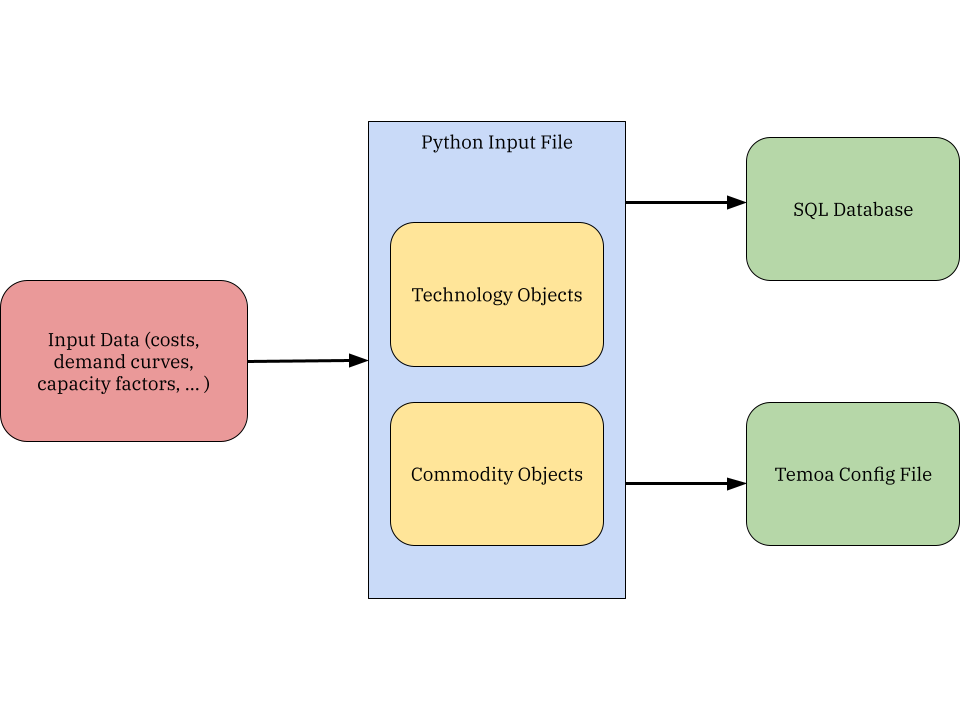
\includegraphics[width=0.8\columnwidth]{figures/pygen-outline.png}
  \caption{The flow of data through \gls{pygen}. \gls{pygen} reads a Python
  input file and writes an \texttt{SQL} database and a configuration textfile.}
  \label{fig:pygen-flow}
\end{figure}
A \gls{pygen} input file can be turned into a template with uncertain parameters
specified using a liquid-text format and then hundreds of input files can be
populated with the \texttt{Jinja2} Python library.

\subsubsection{Time Series Processing}
Automated conversion of continuous time series data into a \gls{temoa}-ready
time slices is one \gls{pygen}' key features. By specifying the number of ``seasons''
and the number of ``times of day,'' users can quickly rerun their model at different
temporal resolutions. The only limit to this is computational tractability on \gls{temoa}'s
end. Figure \ref{fig:solar-timeslice} shows some historical data from \gls{uiuc}'s
first solar farm project, Solar Farm 1.0 \cite{white_solar_2017}, that \gls{pygen}
sliced into four seasons with one representative day of 24 hours each.  
\begin{figure}[H]
  \resizebox{\textwidth}{!}{%% Creator: Matplotlib, PGF backend
%%
%% To include the figure in your LaTeX document, write
%%   \input{<filename>.pgf}
%%
%% Make sure the required packages are loaded in your preamble
%%   \usepackage{pgf}
%%
%% Figures using additional raster images can only be included by \input if
%% they are in the same directory as the main LaTeX file. For loading figures
%% from other directories you can use the `import` package
%%   \usepackage{import}
%%
%% and then include the figures with
%%   \import{<path to file>}{<filename>.pgf}
%%
%% Matplotlib used the following preamble
%%
\begingroup%
\makeatletter%
\begin{pgfpicture}%
\pgfpathrectangle{\pgfpointorigin}{\pgfqpoint{17.900000in}{8.900000in}}%
\pgfusepath{use as bounding box, clip}%
\begin{pgfscope}%
\pgfsetbuttcap%
\pgfsetmiterjoin%
\definecolor{currentfill}{rgb}{1.000000,1.000000,1.000000}%
\pgfsetfillcolor{currentfill}%
\pgfsetlinewidth{0.000000pt}%
\definecolor{currentstroke}{rgb}{0.000000,0.000000,0.000000}%
\pgfsetstrokecolor{currentstroke}%
\pgfsetdash{}{0pt}%
\pgfpathmoveto{\pgfqpoint{0.000000in}{0.000000in}}%
\pgfpathlineto{\pgfqpoint{17.900000in}{0.000000in}}%
\pgfpathlineto{\pgfqpoint{17.900000in}{8.900000in}}%
\pgfpathlineto{\pgfqpoint{0.000000in}{8.900000in}}%
\pgfpathclose%
\pgfusepath{fill}%
\end{pgfscope}%
\begin{pgfscope}%
\pgfsetbuttcap%
\pgfsetmiterjoin%
\definecolor{currentfill}{rgb}{0.898039,0.898039,0.898039}%
\pgfsetfillcolor{currentfill}%
\pgfsetlinewidth{0.000000pt}%
\definecolor{currentstroke}{rgb}{0.000000,0.000000,0.000000}%
\pgfsetstrokecolor{currentstroke}%
\pgfsetstrokeopacity{0.000000}%
\pgfsetdash{}{0pt}%
\pgfpathmoveto{\pgfqpoint{0.931995in}{0.892178in}}%
\pgfpathlineto{\pgfqpoint{12.883221in}{0.892178in}}%
\pgfpathlineto{\pgfqpoint{12.883221in}{8.516628in}}%
\pgfpathlineto{\pgfqpoint{0.931995in}{8.516628in}}%
\pgfpathclose%
\pgfusepath{fill}%
\end{pgfscope}%
\begin{pgfscope}%
\pgfpathrectangle{\pgfqpoint{0.931995in}{0.892178in}}{\pgfqpoint{11.951226in}{7.624450in}}%
\pgfusepath{clip}%
\pgfsetrectcap%
\pgfsetroundjoin%
\pgfsetlinewidth{0.803000pt}%
\definecolor{currentstroke}{rgb}{1.000000,1.000000,1.000000}%
\pgfsetstrokecolor{currentstroke}%
\pgfsetdash{}{0pt}%
\pgfpathmoveto{\pgfqpoint{0.931995in}{0.892178in}}%
\pgfpathlineto{\pgfqpoint{0.931995in}{8.516628in}}%
\pgfusepath{stroke}%
\end{pgfscope}%
\begin{pgfscope}%
\pgfsetbuttcap%
\pgfsetroundjoin%
\definecolor{currentfill}{rgb}{0.333333,0.333333,0.333333}%
\pgfsetfillcolor{currentfill}%
\pgfsetlinewidth{0.803000pt}%
\definecolor{currentstroke}{rgb}{0.333333,0.333333,0.333333}%
\pgfsetstrokecolor{currentstroke}%
\pgfsetdash{}{0pt}%
\pgfsys@defobject{currentmarker}{\pgfqpoint{0.000000in}{-0.048611in}}{\pgfqpoint{0.000000in}{0.000000in}}{%
\pgfpathmoveto{\pgfqpoint{0.000000in}{0.000000in}}%
\pgfpathlineto{\pgfqpoint{0.000000in}{-0.048611in}}%
\pgfusepath{stroke,fill}%
}%
\begin{pgfscope}%
\pgfsys@transformshift{0.931995in}{0.892178in}%
\pgfsys@useobject{currentmarker}{}%
\end{pgfscope}%
\end{pgfscope}%
\begin{pgfscope}%
\definecolor{textcolor}{rgb}{0.333333,0.333333,0.333333}%
\pgfsetstrokecolor{textcolor}%
\pgfsetfillcolor{textcolor}%
\pgftext[x=0.778339in, y=0.656067in, left, base]{\color{textcolor}\rmfamily\fontsize{14.000000}{16.800000}\selectfont Jan}%
\end{pgfscope}%
\begin{pgfscope}%
\definecolor{textcolor}{rgb}{0.333333,0.333333,0.333333}%
\pgfsetstrokecolor{textcolor}%
\pgfsetfillcolor{textcolor}%
\pgftext[x=0.736164in, y=0.450512in, left, base]{\color{textcolor}\rmfamily\fontsize{14.000000}{16.800000}\selectfont 2016}%
\end{pgfscope}%
\begin{pgfscope}%
\pgfpathrectangle{\pgfqpoint{0.931995in}{0.892178in}}{\pgfqpoint{11.951226in}{7.624450in}}%
\pgfusepath{clip}%
\pgfsetrectcap%
\pgfsetroundjoin%
\pgfsetlinewidth{0.803000pt}%
\definecolor{currentstroke}{rgb}{1.000000,1.000000,1.000000}%
\pgfsetstrokecolor{currentstroke}%
\pgfsetdash{}{0pt}%
\pgfpathmoveto{\pgfqpoint{4.923158in}{0.892178in}}%
\pgfpathlineto{\pgfqpoint{4.923158in}{8.516628in}}%
\pgfusepath{stroke}%
\end{pgfscope}%
\begin{pgfscope}%
\pgfsetbuttcap%
\pgfsetroundjoin%
\definecolor{currentfill}{rgb}{0.333333,0.333333,0.333333}%
\pgfsetfillcolor{currentfill}%
\pgfsetlinewidth{0.803000pt}%
\definecolor{currentstroke}{rgb}{0.333333,0.333333,0.333333}%
\pgfsetstrokecolor{currentstroke}%
\pgfsetdash{}{0pt}%
\pgfsys@defobject{currentmarker}{\pgfqpoint{0.000000in}{-0.048611in}}{\pgfqpoint{0.000000in}{0.000000in}}{%
\pgfpathmoveto{\pgfqpoint{0.000000in}{0.000000in}}%
\pgfpathlineto{\pgfqpoint{0.000000in}{-0.048611in}}%
\pgfusepath{stroke,fill}%
}%
\begin{pgfscope}%
\pgfsys@transformshift{4.923158in}{0.892178in}%
\pgfsys@useobject{currentmarker}{}%
\end{pgfscope}%
\end{pgfscope}%
\begin{pgfscope}%
\definecolor{textcolor}{rgb}{0.333333,0.333333,0.333333}%
\pgfsetstrokecolor{textcolor}%
\pgfsetfillcolor{textcolor}%
\pgftext[x=4.769503in, y=0.656067in, left, base]{\color{textcolor}\rmfamily\fontsize{14.000000}{16.800000}\selectfont Jan}%
\end{pgfscope}%
\begin{pgfscope}%
\definecolor{textcolor}{rgb}{0.333333,0.333333,0.333333}%
\pgfsetstrokecolor{textcolor}%
\pgfsetfillcolor{textcolor}%
\pgftext[x=4.727327in, y=0.450512in, left, base]{\color{textcolor}\rmfamily\fontsize{14.000000}{16.800000}\selectfont 2017}%
\end{pgfscope}%
\begin{pgfscope}%
\pgfpathrectangle{\pgfqpoint{0.931995in}{0.892178in}}{\pgfqpoint{11.951226in}{7.624450in}}%
\pgfusepath{clip}%
\pgfsetrectcap%
\pgfsetroundjoin%
\pgfsetlinewidth{0.803000pt}%
\definecolor{currentstroke}{rgb}{1.000000,1.000000,1.000000}%
\pgfsetstrokecolor{currentstroke}%
\pgfsetdash{}{0pt}%
\pgfpathmoveto{\pgfqpoint{8.903417in}{0.892178in}}%
\pgfpathlineto{\pgfqpoint{8.903417in}{8.516628in}}%
\pgfusepath{stroke}%
\end{pgfscope}%
\begin{pgfscope}%
\pgfsetbuttcap%
\pgfsetroundjoin%
\definecolor{currentfill}{rgb}{0.333333,0.333333,0.333333}%
\pgfsetfillcolor{currentfill}%
\pgfsetlinewidth{0.803000pt}%
\definecolor{currentstroke}{rgb}{0.333333,0.333333,0.333333}%
\pgfsetstrokecolor{currentstroke}%
\pgfsetdash{}{0pt}%
\pgfsys@defobject{currentmarker}{\pgfqpoint{0.000000in}{-0.048611in}}{\pgfqpoint{0.000000in}{0.000000in}}{%
\pgfpathmoveto{\pgfqpoint{0.000000in}{0.000000in}}%
\pgfpathlineto{\pgfqpoint{0.000000in}{-0.048611in}}%
\pgfusepath{stroke,fill}%
}%
\begin{pgfscope}%
\pgfsys@transformshift{8.903417in}{0.892178in}%
\pgfsys@useobject{currentmarker}{}%
\end{pgfscope}%
\end{pgfscope}%
\begin{pgfscope}%
\definecolor{textcolor}{rgb}{0.333333,0.333333,0.333333}%
\pgfsetstrokecolor{textcolor}%
\pgfsetfillcolor{textcolor}%
\pgftext[x=8.749761in, y=0.656067in, left, base]{\color{textcolor}\rmfamily\fontsize{14.000000}{16.800000}\selectfont Jan}%
\end{pgfscope}%
\begin{pgfscope}%
\definecolor{textcolor}{rgb}{0.333333,0.333333,0.333333}%
\pgfsetstrokecolor{textcolor}%
\pgfsetfillcolor{textcolor}%
\pgftext[x=8.707586in, y=0.450512in, left, base]{\color{textcolor}\rmfamily\fontsize{14.000000}{16.800000}\selectfont 2018}%
\end{pgfscope}%
\begin{pgfscope}%
\pgfpathrectangle{\pgfqpoint{0.931995in}{0.892178in}}{\pgfqpoint{11.951226in}{7.624450in}}%
\pgfusepath{clip}%
\pgfsetrectcap%
\pgfsetroundjoin%
\pgfsetlinewidth{0.803000pt}%
\definecolor{currentstroke}{rgb}{1.000000,1.000000,1.000000}%
\pgfsetstrokecolor{currentstroke}%
\pgfsetdash{}{0pt}%
\pgfpathmoveto{\pgfqpoint{12.883221in}{0.892178in}}%
\pgfpathlineto{\pgfqpoint{12.883221in}{8.516628in}}%
\pgfusepath{stroke}%
\end{pgfscope}%
\begin{pgfscope}%
\pgfsetbuttcap%
\pgfsetroundjoin%
\definecolor{currentfill}{rgb}{0.333333,0.333333,0.333333}%
\pgfsetfillcolor{currentfill}%
\pgfsetlinewidth{0.803000pt}%
\definecolor{currentstroke}{rgb}{0.333333,0.333333,0.333333}%
\pgfsetstrokecolor{currentstroke}%
\pgfsetdash{}{0pt}%
\pgfsys@defobject{currentmarker}{\pgfqpoint{0.000000in}{-0.048611in}}{\pgfqpoint{0.000000in}{0.000000in}}{%
\pgfpathmoveto{\pgfqpoint{0.000000in}{0.000000in}}%
\pgfpathlineto{\pgfqpoint{0.000000in}{-0.048611in}}%
\pgfusepath{stroke,fill}%
}%
\begin{pgfscope}%
\pgfsys@transformshift{12.883221in}{0.892178in}%
\pgfsys@useobject{currentmarker}{}%
\end{pgfscope}%
\end{pgfscope}%
\begin{pgfscope}%
\pgfpathrectangle{\pgfqpoint{0.931995in}{0.892178in}}{\pgfqpoint{11.951226in}{7.624450in}}%
\pgfusepath{clip}%
\pgfsetbuttcap%
\pgfsetroundjoin%
\pgfsetlinewidth{0.803000pt}%
\definecolor{currentstroke}{rgb}{1.000000,1.000000,1.000000}%
\pgfsetstrokecolor{currentstroke}%
\pgfsetdash{{2.960000pt}{1.280000pt}}{0.000000pt}%
\pgfpathmoveto{\pgfqpoint{1.929786in}{0.892178in}}%
\pgfpathlineto{\pgfqpoint{1.929786in}{8.516628in}}%
\pgfusepath{stroke}%
\end{pgfscope}%
\begin{pgfscope}%
\pgfsetbuttcap%
\pgfsetroundjoin%
\definecolor{currentfill}{rgb}{0.333333,0.333333,0.333333}%
\pgfsetfillcolor{currentfill}%
\pgfsetlinewidth{0.602250pt}%
\definecolor{currentstroke}{rgb}{0.333333,0.333333,0.333333}%
\pgfsetstrokecolor{currentstroke}%
\pgfsetdash{}{0pt}%
\pgfsys@defobject{currentmarker}{\pgfqpoint{0.000000in}{-0.027778in}}{\pgfqpoint{0.000000in}{0.000000in}}{%
\pgfpathmoveto{\pgfqpoint{0.000000in}{0.000000in}}%
\pgfpathlineto{\pgfqpoint{0.000000in}{-0.027778in}}%
\pgfusepath{stroke,fill}%
}%
\begin{pgfscope}%
\pgfsys@transformshift{1.929786in}{0.892178in}%
\pgfsys@useobject{currentmarker}{}%
\end{pgfscope}%
\end{pgfscope}%
\begin{pgfscope}%
\pgfpathrectangle{\pgfqpoint{0.931995in}{0.892178in}}{\pgfqpoint{11.951226in}{7.624450in}}%
\pgfusepath{clip}%
\pgfsetbuttcap%
\pgfsetroundjoin%
\pgfsetlinewidth{0.803000pt}%
\definecolor{currentstroke}{rgb}{1.000000,1.000000,1.000000}%
\pgfsetstrokecolor{currentstroke}%
\pgfsetdash{{2.960000pt}{1.280000pt}}{0.000000pt}%
\pgfpathmoveto{\pgfqpoint{2.927577in}{0.892178in}}%
\pgfpathlineto{\pgfqpoint{2.927577in}{8.516628in}}%
\pgfusepath{stroke}%
\end{pgfscope}%
\begin{pgfscope}%
\pgfsetbuttcap%
\pgfsetroundjoin%
\definecolor{currentfill}{rgb}{0.333333,0.333333,0.333333}%
\pgfsetfillcolor{currentfill}%
\pgfsetlinewidth{0.602250pt}%
\definecolor{currentstroke}{rgb}{0.333333,0.333333,0.333333}%
\pgfsetstrokecolor{currentstroke}%
\pgfsetdash{}{0pt}%
\pgfsys@defobject{currentmarker}{\pgfqpoint{0.000000in}{-0.027778in}}{\pgfqpoint{0.000000in}{0.000000in}}{%
\pgfpathmoveto{\pgfqpoint{0.000000in}{0.000000in}}%
\pgfpathlineto{\pgfqpoint{0.000000in}{-0.027778in}}%
\pgfusepath{stroke,fill}%
}%
\begin{pgfscope}%
\pgfsys@transformshift{2.927577in}{0.892178in}%
\pgfsys@useobject{currentmarker}{}%
\end{pgfscope}%
\end{pgfscope}%
\begin{pgfscope}%
\pgfpathrectangle{\pgfqpoint{0.931995in}{0.892178in}}{\pgfqpoint{11.951226in}{7.624450in}}%
\pgfusepath{clip}%
\pgfsetbuttcap%
\pgfsetroundjoin%
\pgfsetlinewidth{0.803000pt}%
\definecolor{currentstroke}{rgb}{1.000000,1.000000,1.000000}%
\pgfsetstrokecolor{currentstroke}%
\pgfsetdash{{2.960000pt}{1.280000pt}}{0.000000pt}%
\pgfpathmoveto{\pgfqpoint{3.925367in}{0.892178in}}%
\pgfpathlineto{\pgfqpoint{3.925367in}{8.516628in}}%
\pgfusepath{stroke}%
\end{pgfscope}%
\begin{pgfscope}%
\pgfsetbuttcap%
\pgfsetroundjoin%
\definecolor{currentfill}{rgb}{0.333333,0.333333,0.333333}%
\pgfsetfillcolor{currentfill}%
\pgfsetlinewidth{0.602250pt}%
\definecolor{currentstroke}{rgb}{0.333333,0.333333,0.333333}%
\pgfsetstrokecolor{currentstroke}%
\pgfsetdash{}{0pt}%
\pgfsys@defobject{currentmarker}{\pgfqpoint{0.000000in}{-0.027778in}}{\pgfqpoint{0.000000in}{0.000000in}}{%
\pgfpathmoveto{\pgfqpoint{0.000000in}{0.000000in}}%
\pgfpathlineto{\pgfqpoint{0.000000in}{-0.027778in}}%
\pgfusepath{stroke,fill}%
}%
\begin{pgfscope}%
\pgfsys@transformshift{3.925367in}{0.892178in}%
\pgfsys@useobject{currentmarker}{}%
\end{pgfscope}%
\end{pgfscope}%
\begin{pgfscope}%
\pgfpathrectangle{\pgfqpoint{0.931995in}{0.892178in}}{\pgfqpoint{11.951226in}{7.624450in}}%
\pgfusepath{clip}%
\pgfsetbuttcap%
\pgfsetroundjoin%
\pgfsetlinewidth{0.803000pt}%
\definecolor{currentstroke}{rgb}{1.000000,1.000000,1.000000}%
\pgfsetstrokecolor{currentstroke}%
\pgfsetdash{{2.960000pt}{1.280000pt}}{0.000000pt}%
\pgfpathmoveto{\pgfqpoint{5.920949in}{0.892178in}}%
\pgfpathlineto{\pgfqpoint{5.920949in}{8.516628in}}%
\pgfusepath{stroke}%
\end{pgfscope}%
\begin{pgfscope}%
\pgfsetbuttcap%
\pgfsetroundjoin%
\definecolor{currentfill}{rgb}{0.333333,0.333333,0.333333}%
\pgfsetfillcolor{currentfill}%
\pgfsetlinewidth{0.602250pt}%
\definecolor{currentstroke}{rgb}{0.333333,0.333333,0.333333}%
\pgfsetstrokecolor{currentstroke}%
\pgfsetdash{}{0pt}%
\pgfsys@defobject{currentmarker}{\pgfqpoint{0.000000in}{-0.027778in}}{\pgfqpoint{0.000000in}{0.000000in}}{%
\pgfpathmoveto{\pgfqpoint{0.000000in}{0.000000in}}%
\pgfpathlineto{\pgfqpoint{0.000000in}{-0.027778in}}%
\pgfusepath{stroke,fill}%
}%
\begin{pgfscope}%
\pgfsys@transformshift{5.920949in}{0.892178in}%
\pgfsys@useobject{currentmarker}{}%
\end{pgfscope}%
\end{pgfscope}%
\begin{pgfscope}%
\pgfpathrectangle{\pgfqpoint{0.931995in}{0.892178in}}{\pgfqpoint{11.951226in}{7.624450in}}%
\pgfusepath{clip}%
\pgfsetbuttcap%
\pgfsetroundjoin%
\pgfsetlinewidth{0.803000pt}%
\definecolor{currentstroke}{rgb}{1.000000,1.000000,1.000000}%
\pgfsetstrokecolor{currentstroke}%
\pgfsetdash{{2.960000pt}{1.280000pt}}{0.000000pt}%
\pgfpathmoveto{\pgfqpoint{6.918740in}{0.892178in}}%
\pgfpathlineto{\pgfqpoint{6.918740in}{8.516628in}}%
\pgfusepath{stroke}%
\end{pgfscope}%
\begin{pgfscope}%
\pgfsetbuttcap%
\pgfsetroundjoin%
\definecolor{currentfill}{rgb}{0.333333,0.333333,0.333333}%
\pgfsetfillcolor{currentfill}%
\pgfsetlinewidth{0.602250pt}%
\definecolor{currentstroke}{rgb}{0.333333,0.333333,0.333333}%
\pgfsetstrokecolor{currentstroke}%
\pgfsetdash{}{0pt}%
\pgfsys@defobject{currentmarker}{\pgfqpoint{0.000000in}{-0.027778in}}{\pgfqpoint{0.000000in}{0.000000in}}{%
\pgfpathmoveto{\pgfqpoint{0.000000in}{0.000000in}}%
\pgfpathlineto{\pgfqpoint{0.000000in}{-0.027778in}}%
\pgfusepath{stroke,fill}%
}%
\begin{pgfscope}%
\pgfsys@transformshift{6.918740in}{0.892178in}%
\pgfsys@useobject{currentmarker}{}%
\end{pgfscope}%
\end{pgfscope}%
\begin{pgfscope}%
\pgfpathrectangle{\pgfqpoint{0.931995in}{0.892178in}}{\pgfqpoint{11.951226in}{7.624450in}}%
\pgfusepath{clip}%
\pgfsetbuttcap%
\pgfsetroundjoin%
\pgfsetlinewidth{0.803000pt}%
\definecolor{currentstroke}{rgb}{1.000000,1.000000,1.000000}%
\pgfsetstrokecolor{currentstroke}%
\pgfsetdash{{2.960000pt}{1.280000pt}}{0.000000pt}%
\pgfpathmoveto{\pgfqpoint{7.916531in}{0.892178in}}%
\pgfpathlineto{\pgfqpoint{7.916531in}{8.516628in}}%
\pgfusepath{stroke}%
\end{pgfscope}%
\begin{pgfscope}%
\pgfsetbuttcap%
\pgfsetroundjoin%
\definecolor{currentfill}{rgb}{0.333333,0.333333,0.333333}%
\pgfsetfillcolor{currentfill}%
\pgfsetlinewidth{0.602250pt}%
\definecolor{currentstroke}{rgb}{0.333333,0.333333,0.333333}%
\pgfsetstrokecolor{currentstroke}%
\pgfsetdash{}{0pt}%
\pgfsys@defobject{currentmarker}{\pgfqpoint{0.000000in}{-0.027778in}}{\pgfqpoint{0.000000in}{0.000000in}}{%
\pgfpathmoveto{\pgfqpoint{0.000000in}{0.000000in}}%
\pgfpathlineto{\pgfqpoint{0.000000in}{-0.027778in}}%
\pgfusepath{stroke,fill}%
}%
\begin{pgfscope}%
\pgfsys@transformshift{7.916531in}{0.892178in}%
\pgfsys@useobject{currentmarker}{}%
\end{pgfscope}%
\end{pgfscope}%
\begin{pgfscope}%
\pgfpathrectangle{\pgfqpoint{0.931995in}{0.892178in}}{\pgfqpoint{11.951226in}{7.624450in}}%
\pgfusepath{clip}%
\pgfsetbuttcap%
\pgfsetroundjoin%
\pgfsetlinewidth{0.803000pt}%
\definecolor{currentstroke}{rgb}{1.000000,1.000000,1.000000}%
\pgfsetstrokecolor{currentstroke}%
\pgfsetdash{{2.960000pt}{1.280000pt}}{0.000000pt}%
\pgfpathmoveto{\pgfqpoint{8.914322in}{0.892178in}}%
\pgfpathlineto{\pgfqpoint{8.914322in}{8.516628in}}%
\pgfusepath{stroke}%
\end{pgfscope}%
\begin{pgfscope}%
\pgfsetbuttcap%
\pgfsetroundjoin%
\definecolor{currentfill}{rgb}{0.333333,0.333333,0.333333}%
\pgfsetfillcolor{currentfill}%
\pgfsetlinewidth{0.602250pt}%
\definecolor{currentstroke}{rgb}{0.333333,0.333333,0.333333}%
\pgfsetstrokecolor{currentstroke}%
\pgfsetdash{}{0pt}%
\pgfsys@defobject{currentmarker}{\pgfqpoint{0.000000in}{-0.027778in}}{\pgfqpoint{0.000000in}{0.000000in}}{%
\pgfpathmoveto{\pgfqpoint{0.000000in}{0.000000in}}%
\pgfpathlineto{\pgfqpoint{0.000000in}{-0.027778in}}%
\pgfusepath{stroke,fill}%
}%
\begin{pgfscope}%
\pgfsys@transformshift{8.914322in}{0.892178in}%
\pgfsys@useobject{currentmarker}{}%
\end{pgfscope}%
\end{pgfscope}%
\begin{pgfscope}%
\pgfpathrectangle{\pgfqpoint{0.931995in}{0.892178in}}{\pgfqpoint{11.951226in}{7.624450in}}%
\pgfusepath{clip}%
\pgfsetbuttcap%
\pgfsetroundjoin%
\pgfsetlinewidth{0.803000pt}%
\definecolor{currentstroke}{rgb}{1.000000,1.000000,1.000000}%
\pgfsetstrokecolor{currentstroke}%
\pgfsetdash{{2.960000pt}{1.280000pt}}{0.000000pt}%
\pgfpathmoveto{\pgfqpoint{9.912112in}{0.892178in}}%
\pgfpathlineto{\pgfqpoint{9.912112in}{8.516628in}}%
\pgfusepath{stroke}%
\end{pgfscope}%
\begin{pgfscope}%
\pgfsetbuttcap%
\pgfsetroundjoin%
\definecolor{currentfill}{rgb}{0.333333,0.333333,0.333333}%
\pgfsetfillcolor{currentfill}%
\pgfsetlinewidth{0.602250pt}%
\definecolor{currentstroke}{rgb}{0.333333,0.333333,0.333333}%
\pgfsetstrokecolor{currentstroke}%
\pgfsetdash{}{0pt}%
\pgfsys@defobject{currentmarker}{\pgfqpoint{0.000000in}{-0.027778in}}{\pgfqpoint{0.000000in}{0.000000in}}{%
\pgfpathmoveto{\pgfqpoint{0.000000in}{0.000000in}}%
\pgfpathlineto{\pgfqpoint{0.000000in}{-0.027778in}}%
\pgfusepath{stroke,fill}%
}%
\begin{pgfscope}%
\pgfsys@transformshift{9.912112in}{0.892178in}%
\pgfsys@useobject{currentmarker}{}%
\end{pgfscope}%
\end{pgfscope}%
\begin{pgfscope}%
\pgfpathrectangle{\pgfqpoint{0.931995in}{0.892178in}}{\pgfqpoint{11.951226in}{7.624450in}}%
\pgfusepath{clip}%
\pgfsetbuttcap%
\pgfsetroundjoin%
\pgfsetlinewidth{0.803000pt}%
\definecolor{currentstroke}{rgb}{1.000000,1.000000,1.000000}%
\pgfsetstrokecolor{currentstroke}%
\pgfsetdash{{2.960000pt}{1.280000pt}}{0.000000pt}%
\pgfpathmoveto{\pgfqpoint{10.909903in}{0.892178in}}%
\pgfpathlineto{\pgfqpoint{10.909903in}{8.516628in}}%
\pgfusepath{stroke}%
\end{pgfscope}%
\begin{pgfscope}%
\pgfsetbuttcap%
\pgfsetroundjoin%
\definecolor{currentfill}{rgb}{0.333333,0.333333,0.333333}%
\pgfsetfillcolor{currentfill}%
\pgfsetlinewidth{0.602250pt}%
\definecolor{currentstroke}{rgb}{0.333333,0.333333,0.333333}%
\pgfsetstrokecolor{currentstroke}%
\pgfsetdash{}{0pt}%
\pgfsys@defobject{currentmarker}{\pgfqpoint{0.000000in}{-0.027778in}}{\pgfqpoint{0.000000in}{0.000000in}}{%
\pgfpathmoveto{\pgfqpoint{0.000000in}{0.000000in}}%
\pgfpathlineto{\pgfqpoint{0.000000in}{-0.027778in}}%
\pgfusepath{stroke,fill}%
}%
\begin{pgfscope}%
\pgfsys@transformshift{10.909903in}{0.892178in}%
\pgfsys@useobject{currentmarker}{}%
\end{pgfscope}%
\end{pgfscope}%
\begin{pgfscope}%
\pgfpathrectangle{\pgfqpoint{0.931995in}{0.892178in}}{\pgfqpoint{11.951226in}{7.624450in}}%
\pgfusepath{clip}%
\pgfsetbuttcap%
\pgfsetroundjoin%
\pgfsetlinewidth{0.803000pt}%
\definecolor{currentstroke}{rgb}{1.000000,1.000000,1.000000}%
\pgfsetstrokecolor{currentstroke}%
\pgfsetdash{{2.960000pt}{1.280000pt}}{0.000000pt}%
\pgfpathmoveto{\pgfqpoint{11.907694in}{0.892178in}}%
\pgfpathlineto{\pgfqpoint{11.907694in}{8.516628in}}%
\pgfusepath{stroke}%
\end{pgfscope}%
\begin{pgfscope}%
\pgfsetbuttcap%
\pgfsetroundjoin%
\definecolor{currentfill}{rgb}{0.333333,0.333333,0.333333}%
\pgfsetfillcolor{currentfill}%
\pgfsetlinewidth{0.602250pt}%
\definecolor{currentstroke}{rgb}{0.333333,0.333333,0.333333}%
\pgfsetstrokecolor{currentstroke}%
\pgfsetdash{}{0pt}%
\pgfsys@defobject{currentmarker}{\pgfqpoint{0.000000in}{-0.027778in}}{\pgfqpoint{0.000000in}{0.000000in}}{%
\pgfpathmoveto{\pgfqpoint{0.000000in}{0.000000in}}%
\pgfpathlineto{\pgfqpoint{0.000000in}{-0.027778in}}%
\pgfusepath{stroke,fill}%
}%
\begin{pgfscope}%
\pgfsys@transformshift{11.907694in}{0.892178in}%
\pgfsys@useobject{currentmarker}{}%
\end{pgfscope}%
\end{pgfscope}%
\begin{pgfscope}%
\definecolor{textcolor}{rgb}{0.333333,0.333333,0.333333}%
\pgfsetstrokecolor{textcolor}%
\pgfsetfillcolor{textcolor}%
\pgftext[x=6.907608in,y=0.356068in,,top]{\color{textcolor}\rmfamily\fontsize{20.000000}{24.000000}\selectfont Date}%
\end{pgfscope}%
\begin{pgfscope}%
\pgfpathrectangle{\pgfqpoint{0.931995in}{0.892178in}}{\pgfqpoint{11.951226in}{7.624450in}}%
\pgfusepath{clip}%
\pgfsetrectcap%
\pgfsetroundjoin%
\pgfsetlinewidth{0.803000pt}%
\definecolor{currentstroke}{rgb}{1.000000,1.000000,1.000000}%
\pgfsetstrokecolor{currentstroke}%
\pgfsetdash{}{0pt}%
\pgfpathmoveto{\pgfqpoint{0.931995in}{0.892178in}}%
\pgfpathlineto{\pgfqpoint{12.883221in}{0.892178in}}%
\pgfusepath{stroke}%
\end{pgfscope}%
\begin{pgfscope}%
\pgfsetbuttcap%
\pgfsetroundjoin%
\definecolor{currentfill}{rgb}{0.333333,0.333333,0.333333}%
\pgfsetfillcolor{currentfill}%
\pgfsetlinewidth{0.803000pt}%
\definecolor{currentstroke}{rgb}{0.333333,0.333333,0.333333}%
\pgfsetstrokecolor{currentstroke}%
\pgfsetdash{}{0pt}%
\pgfsys@defobject{currentmarker}{\pgfqpoint{-0.048611in}{0.000000in}}{\pgfqpoint{-0.000000in}{0.000000in}}{%
\pgfpathmoveto{\pgfqpoint{-0.000000in}{0.000000in}}%
\pgfpathlineto{\pgfqpoint{-0.048611in}{0.000000in}}%
\pgfusepath{stroke,fill}%
}%
\begin{pgfscope}%
\pgfsys@transformshift{0.931995in}{0.892178in}%
\pgfsys@useobject{currentmarker}{}%
\end{pgfscope}%
\end{pgfscope}%
\begin{pgfscope}%
\definecolor{textcolor}{rgb}{0.333333,0.333333,0.333333}%
\pgfsetstrokecolor{textcolor}%
\pgfsetfillcolor{textcolor}%
\pgftext[x=0.736857in, y=0.822734in, left, base]{\color{textcolor}\rmfamily\fontsize{14.000000}{16.800000}\selectfont \(\displaystyle {0}\)}%
\end{pgfscope}%
\begin{pgfscope}%
\pgfpathrectangle{\pgfqpoint{0.931995in}{0.892178in}}{\pgfqpoint{11.951226in}{7.624450in}}%
\pgfusepath{clip}%
\pgfsetrectcap%
\pgfsetroundjoin%
\pgfsetlinewidth{0.803000pt}%
\definecolor{currentstroke}{rgb}{1.000000,1.000000,1.000000}%
\pgfsetstrokecolor{currentstroke}%
\pgfsetdash{}{0pt}%
\pgfpathmoveto{\pgfqpoint{0.931995in}{2.503006in}}%
\pgfpathlineto{\pgfqpoint{12.883221in}{2.503006in}}%
\pgfusepath{stroke}%
\end{pgfscope}%
\begin{pgfscope}%
\pgfsetbuttcap%
\pgfsetroundjoin%
\definecolor{currentfill}{rgb}{0.333333,0.333333,0.333333}%
\pgfsetfillcolor{currentfill}%
\pgfsetlinewidth{0.803000pt}%
\definecolor{currentstroke}{rgb}{0.333333,0.333333,0.333333}%
\pgfsetstrokecolor{currentstroke}%
\pgfsetdash{}{0pt}%
\pgfsys@defobject{currentmarker}{\pgfqpoint{-0.048611in}{0.000000in}}{\pgfqpoint{-0.000000in}{0.000000in}}{%
\pgfpathmoveto{\pgfqpoint{-0.000000in}{0.000000in}}%
\pgfpathlineto{\pgfqpoint{-0.048611in}{0.000000in}}%
\pgfusepath{stroke,fill}%
}%
\begin{pgfscope}%
\pgfsys@transformshift{0.931995in}{2.503006in}%
\pgfsys@useobject{currentmarker}{}%
\end{pgfscope}%
\end{pgfscope}%
\begin{pgfscope}%
\definecolor{textcolor}{rgb}{0.333333,0.333333,0.333333}%
\pgfsetstrokecolor{textcolor}%
\pgfsetfillcolor{textcolor}%
\pgftext[x=0.443111in, y=2.433561in, left, base]{\color{textcolor}\rmfamily\fontsize{14.000000}{16.800000}\selectfont \(\displaystyle {1000}\)}%
\end{pgfscope}%
\begin{pgfscope}%
\pgfpathrectangle{\pgfqpoint{0.931995in}{0.892178in}}{\pgfqpoint{11.951226in}{7.624450in}}%
\pgfusepath{clip}%
\pgfsetrectcap%
\pgfsetroundjoin%
\pgfsetlinewidth{0.803000pt}%
\definecolor{currentstroke}{rgb}{1.000000,1.000000,1.000000}%
\pgfsetstrokecolor{currentstroke}%
\pgfsetdash{}{0pt}%
\pgfpathmoveto{\pgfqpoint{0.931995in}{4.113833in}}%
\pgfpathlineto{\pgfqpoint{12.883221in}{4.113833in}}%
\pgfusepath{stroke}%
\end{pgfscope}%
\begin{pgfscope}%
\pgfsetbuttcap%
\pgfsetroundjoin%
\definecolor{currentfill}{rgb}{0.333333,0.333333,0.333333}%
\pgfsetfillcolor{currentfill}%
\pgfsetlinewidth{0.803000pt}%
\definecolor{currentstroke}{rgb}{0.333333,0.333333,0.333333}%
\pgfsetstrokecolor{currentstroke}%
\pgfsetdash{}{0pt}%
\pgfsys@defobject{currentmarker}{\pgfqpoint{-0.048611in}{0.000000in}}{\pgfqpoint{-0.000000in}{0.000000in}}{%
\pgfpathmoveto{\pgfqpoint{-0.000000in}{0.000000in}}%
\pgfpathlineto{\pgfqpoint{-0.048611in}{0.000000in}}%
\pgfusepath{stroke,fill}%
}%
\begin{pgfscope}%
\pgfsys@transformshift{0.931995in}{4.113833in}%
\pgfsys@useobject{currentmarker}{}%
\end{pgfscope}%
\end{pgfscope}%
\begin{pgfscope}%
\definecolor{textcolor}{rgb}{0.333333,0.333333,0.333333}%
\pgfsetstrokecolor{textcolor}%
\pgfsetfillcolor{textcolor}%
\pgftext[x=0.443111in, y=4.044389in, left, base]{\color{textcolor}\rmfamily\fontsize{14.000000}{16.800000}\selectfont \(\displaystyle {2000}\)}%
\end{pgfscope}%
\begin{pgfscope}%
\pgfpathrectangle{\pgfqpoint{0.931995in}{0.892178in}}{\pgfqpoint{11.951226in}{7.624450in}}%
\pgfusepath{clip}%
\pgfsetrectcap%
\pgfsetroundjoin%
\pgfsetlinewidth{0.803000pt}%
\definecolor{currentstroke}{rgb}{1.000000,1.000000,1.000000}%
\pgfsetstrokecolor{currentstroke}%
\pgfsetdash{}{0pt}%
\pgfpathmoveto{\pgfqpoint{0.931995in}{5.724661in}}%
\pgfpathlineto{\pgfqpoint{12.883221in}{5.724661in}}%
\pgfusepath{stroke}%
\end{pgfscope}%
\begin{pgfscope}%
\pgfsetbuttcap%
\pgfsetroundjoin%
\definecolor{currentfill}{rgb}{0.333333,0.333333,0.333333}%
\pgfsetfillcolor{currentfill}%
\pgfsetlinewidth{0.803000pt}%
\definecolor{currentstroke}{rgb}{0.333333,0.333333,0.333333}%
\pgfsetstrokecolor{currentstroke}%
\pgfsetdash{}{0pt}%
\pgfsys@defobject{currentmarker}{\pgfqpoint{-0.048611in}{0.000000in}}{\pgfqpoint{-0.000000in}{0.000000in}}{%
\pgfpathmoveto{\pgfqpoint{-0.000000in}{0.000000in}}%
\pgfpathlineto{\pgfqpoint{-0.048611in}{0.000000in}}%
\pgfusepath{stroke,fill}%
}%
\begin{pgfscope}%
\pgfsys@transformshift{0.931995in}{5.724661in}%
\pgfsys@useobject{currentmarker}{}%
\end{pgfscope}%
\end{pgfscope}%
\begin{pgfscope}%
\definecolor{textcolor}{rgb}{0.333333,0.333333,0.333333}%
\pgfsetstrokecolor{textcolor}%
\pgfsetfillcolor{textcolor}%
\pgftext[x=0.443111in, y=5.655217in, left, base]{\color{textcolor}\rmfamily\fontsize{14.000000}{16.800000}\selectfont \(\displaystyle {3000}\)}%
\end{pgfscope}%
\begin{pgfscope}%
\pgfpathrectangle{\pgfqpoint{0.931995in}{0.892178in}}{\pgfqpoint{11.951226in}{7.624450in}}%
\pgfusepath{clip}%
\pgfsetrectcap%
\pgfsetroundjoin%
\pgfsetlinewidth{0.803000pt}%
\definecolor{currentstroke}{rgb}{1.000000,1.000000,1.000000}%
\pgfsetstrokecolor{currentstroke}%
\pgfsetdash{}{0pt}%
\pgfpathmoveto{\pgfqpoint{0.931995in}{7.335489in}}%
\pgfpathlineto{\pgfqpoint{12.883221in}{7.335489in}}%
\pgfusepath{stroke}%
\end{pgfscope}%
\begin{pgfscope}%
\pgfsetbuttcap%
\pgfsetroundjoin%
\definecolor{currentfill}{rgb}{0.333333,0.333333,0.333333}%
\pgfsetfillcolor{currentfill}%
\pgfsetlinewidth{0.803000pt}%
\definecolor{currentstroke}{rgb}{0.333333,0.333333,0.333333}%
\pgfsetstrokecolor{currentstroke}%
\pgfsetdash{}{0pt}%
\pgfsys@defobject{currentmarker}{\pgfqpoint{-0.048611in}{0.000000in}}{\pgfqpoint{-0.000000in}{0.000000in}}{%
\pgfpathmoveto{\pgfqpoint{-0.000000in}{0.000000in}}%
\pgfpathlineto{\pgfqpoint{-0.048611in}{0.000000in}}%
\pgfusepath{stroke,fill}%
}%
\begin{pgfscope}%
\pgfsys@transformshift{0.931995in}{7.335489in}%
\pgfsys@useobject{currentmarker}{}%
\end{pgfscope}%
\end{pgfscope}%
\begin{pgfscope}%
\definecolor{textcolor}{rgb}{0.333333,0.333333,0.333333}%
\pgfsetstrokecolor{textcolor}%
\pgfsetfillcolor{textcolor}%
\pgftext[x=0.443111in, y=7.266044in, left, base]{\color{textcolor}\rmfamily\fontsize{14.000000}{16.800000}\selectfont \(\displaystyle {4000}\)}%
\end{pgfscope}%
\begin{pgfscope}%
\pgfpathrectangle{\pgfqpoint{0.931995in}{0.892178in}}{\pgfqpoint{11.951226in}{7.624450in}}%
\pgfusepath{clip}%
\pgfsetbuttcap%
\pgfsetroundjoin%
\pgfsetlinewidth{0.803000pt}%
\definecolor{currentstroke}{rgb}{1.000000,1.000000,1.000000}%
\pgfsetstrokecolor{currentstroke}%
\pgfsetdash{{2.960000pt}{1.280000pt}}{0.000000pt}%
\pgfpathmoveto{\pgfqpoint{0.931995in}{1.214343in}}%
\pgfpathlineto{\pgfqpoint{12.883221in}{1.214343in}}%
\pgfusepath{stroke}%
\end{pgfscope}%
\begin{pgfscope}%
\pgfsetbuttcap%
\pgfsetroundjoin%
\definecolor{currentfill}{rgb}{0.333333,0.333333,0.333333}%
\pgfsetfillcolor{currentfill}%
\pgfsetlinewidth{0.602250pt}%
\definecolor{currentstroke}{rgb}{0.333333,0.333333,0.333333}%
\pgfsetstrokecolor{currentstroke}%
\pgfsetdash{}{0pt}%
\pgfsys@defobject{currentmarker}{\pgfqpoint{-0.027778in}{0.000000in}}{\pgfqpoint{-0.000000in}{0.000000in}}{%
\pgfpathmoveto{\pgfqpoint{-0.000000in}{0.000000in}}%
\pgfpathlineto{\pgfqpoint{-0.027778in}{0.000000in}}%
\pgfusepath{stroke,fill}%
}%
\begin{pgfscope}%
\pgfsys@transformshift{0.931995in}{1.214343in}%
\pgfsys@useobject{currentmarker}{}%
\end{pgfscope}%
\end{pgfscope}%
\begin{pgfscope}%
\pgfpathrectangle{\pgfqpoint{0.931995in}{0.892178in}}{\pgfqpoint{11.951226in}{7.624450in}}%
\pgfusepath{clip}%
\pgfsetbuttcap%
\pgfsetroundjoin%
\pgfsetlinewidth{0.803000pt}%
\definecolor{currentstroke}{rgb}{1.000000,1.000000,1.000000}%
\pgfsetstrokecolor{currentstroke}%
\pgfsetdash{{2.960000pt}{1.280000pt}}{0.000000pt}%
\pgfpathmoveto{\pgfqpoint{0.931995in}{1.536509in}}%
\pgfpathlineto{\pgfqpoint{12.883221in}{1.536509in}}%
\pgfusepath{stroke}%
\end{pgfscope}%
\begin{pgfscope}%
\pgfsetbuttcap%
\pgfsetroundjoin%
\definecolor{currentfill}{rgb}{0.333333,0.333333,0.333333}%
\pgfsetfillcolor{currentfill}%
\pgfsetlinewidth{0.602250pt}%
\definecolor{currentstroke}{rgb}{0.333333,0.333333,0.333333}%
\pgfsetstrokecolor{currentstroke}%
\pgfsetdash{}{0pt}%
\pgfsys@defobject{currentmarker}{\pgfqpoint{-0.027778in}{0.000000in}}{\pgfqpoint{-0.000000in}{0.000000in}}{%
\pgfpathmoveto{\pgfqpoint{-0.000000in}{0.000000in}}%
\pgfpathlineto{\pgfqpoint{-0.027778in}{0.000000in}}%
\pgfusepath{stroke,fill}%
}%
\begin{pgfscope}%
\pgfsys@transformshift{0.931995in}{1.536509in}%
\pgfsys@useobject{currentmarker}{}%
\end{pgfscope}%
\end{pgfscope}%
\begin{pgfscope}%
\pgfpathrectangle{\pgfqpoint{0.931995in}{0.892178in}}{\pgfqpoint{11.951226in}{7.624450in}}%
\pgfusepath{clip}%
\pgfsetbuttcap%
\pgfsetroundjoin%
\pgfsetlinewidth{0.803000pt}%
\definecolor{currentstroke}{rgb}{1.000000,1.000000,1.000000}%
\pgfsetstrokecolor{currentstroke}%
\pgfsetdash{{2.960000pt}{1.280000pt}}{0.000000pt}%
\pgfpathmoveto{\pgfqpoint{0.931995in}{1.858674in}}%
\pgfpathlineto{\pgfqpoint{12.883221in}{1.858674in}}%
\pgfusepath{stroke}%
\end{pgfscope}%
\begin{pgfscope}%
\pgfsetbuttcap%
\pgfsetroundjoin%
\definecolor{currentfill}{rgb}{0.333333,0.333333,0.333333}%
\pgfsetfillcolor{currentfill}%
\pgfsetlinewidth{0.602250pt}%
\definecolor{currentstroke}{rgb}{0.333333,0.333333,0.333333}%
\pgfsetstrokecolor{currentstroke}%
\pgfsetdash{}{0pt}%
\pgfsys@defobject{currentmarker}{\pgfqpoint{-0.027778in}{0.000000in}}{\pgfqpoint{-0.000000in}{0.000000in}}{%
\pgfpathmoveto{\pgfqpoint{-0.000000in}{0.000000in}}%
\pgfpathlineto{\pgfqpoint{-0.027778in}{0.000000in}}%
\pgfusepath{stroke,fill}%
}%
\begin{pgfscope}%
\pgfsys@transformshift{0.931995in}{1.858674in}%
\pgfsys@useobject{currentmarker}{}%
\end{pgfscope}%
\end{pgfscope}%
\begin{pgfscope}%
\pgfpathrectangle{\pgfqpoint{0.931995in}{0.892178in}}{\pgfqpoint{11.951226in}{7.624450in}}%
\pgfusepath{clip}%
\pgfsetbuttcap%
\pgfsetroundjoin%
\pgfsetlinewidth{0.803000pt}%
\definecolor{currentstroke}{rgb}{1.000000,1.000000,1.000000}%
\pgfsetstrokecolor{currentstroke}%
\pgfsetdash{{2.960000pt}{1.280000pt}}{0.000000pt}%
\pgfpathmoveto{\pgfqpoint{0.931995in}{2.180840in}}%
\pgfpathlineto{\pgfqpoint{12.883221in}{2.180840in}}%
\pgfusepath{stroke}%
\end{pgfscope}%
\begin{pgfscope}%
\pgfsetbuttcap%
\pgfsetroundjoin%
\definecolor{currentfill}{rgb}{0.333333,0.333333,0.333333}%
\pgfsetfillcolor{currentfill}%
\pgfsetlinewidth{0.602250pt}%
\definecolor{currentstroke}{rgb}{0.333333,0.333333,0.333333}%
\pgfsetstrokecolor{currentstroke}%
\pgfsetdash{}{0pt}%
\pgfsys@defobject{currentmarker}{\pgfqpoint{-0.027778in}{0.000000in}}{\pgfqpoint{-0.000000in}{0.000000in}}{%
\pgfpathmoveto{\pgfqpoint{-0.000000in}{0.000000in}}%
\pgfpathlineto{\pgfqpoint{-0.027778in}{0.000000in}}%
\pgfusepath{stroke,fill}%
}%
\begin{pgfscope}%
\pgfsys@transformshift{0.931995in}{2.180840in}%
\pgfsys@useobject{currentmarker}{}%
\end{pgfscope}%
\end{pgfscope}%
\begin{pgfscope}%
\pgfpathrectangle{\pgfqpoint{0.931995in}{0.892178in}}{\pgfqpoint{11.951226in}{7.624450in}}%
\pgfusepath{clip}%
\pgfsetbuttcap%
\pgfsetroundjoin%
\pgfsetlinewidth{0.803000pt}%
\definecolor{currentstroke}{rgb}{1.000000,1.000000,1.000000}%
\pgfsetstrokecolor{currentstroke}%
\pgfsetdash{{2.960000pt}{1.280000pt}}{0.000000pt}%
\pgfpathmoveto{\pgfqpoint{0.931995in}{2.825171in}}%
\pgfpathlineto{\pgfqpoint{12.883221in}{2.825171in}}%
\pgfusepath{stroke}%
\end{pgfscope}%
\begin{pgfscope}%
\pgfsetbuttcap%
\pgfsetroundjoin%
\definecolor{currentfill}{rgb}{0.333333,0.333333,0.333333}%
\pgfsetfillcolor{currentfill}%
\pgfsetlinewidth{0.602250pt}%
\definecolor{currentstroke}{rgb}{0.333333,0.333333,0.333333}%
\pgfsetstrokecolor{currentstroke}%
\pgfsetdash{}{0pt}%
\pgfsys@defobject{currentmarker}{\pgfqpoint{-0.027778in}{0.000000in}}{\pgfqpoint{-0.000000in}{0.000000in}}{%
\pgfpathmoveto{\pgfqpoint{-0.000000in}{0.000000in}}%
\pgfpathlineto{\pgfqpoint{-0.027778in}{0.000000in}}%
\pgfusepath{stroke,fill}%
}%
\begin{pgfscope}%
\pgfsys@transformshift{0.931995in}{2.825171in}%
\pgfsys@useobject{currentmarker}{}%
\end{pgfscope}%
\end{pgfscope}%
\begin{pgfscope}%
\pgfpathrectangle{\pgfqpoint{0.931995in}{0.892178in}}{\pgfqpoint{11.951226in}{7.624450in}}%
\pgfusepath{clip}%
\pgfsetbuttcap%
\pgfsetroundjoin%
\pgfsetlinewidth{0.803000pt}%
\definecolor{currentstroke}{rgb}{1.000000,1.000000,1.000000}%
\pgfsetstrokecolor{currentstroke}%
\pgfsetdash{{2.960000pt}{1.280000pt}}{0.000000pt}%
\pgfpathmoveto{\pgfqpoint{0.931995in}{3.147337in}}%
\pgfpathlineto{\pgfqpoint{12.883221in}{3.147337in}}%
\pgfusepath{stroke}%
\end{pgfscope}%
\begin{pgfscope}%
\pgfsetbuttcap%
\pgfsetroundjoin%
\definecolor{currentfill}{rgb}{0.333333,0.333333,0.333333}%
\pgfsetfillcolor{currentfill}%
\pgfsetlinewidth{0.602250pt}%
\definecolor{currentstroke}{rgb}{0.333333,0.333333,0.333333}%
\pgfsetstrokecolor{currentstroke}%
\pgfsetdash{}{0pt}%
\pgfsys@defobject{currentmarker}{\pgfqpoint{-0.027778in}{0.000000in}}{\pgfqpoint{-0.000000in}{0.000000in}}{%
\pgfpathmoveto{\pgfqpoint{-0.000000in}{0.000000in}}%
\pgfpathlineto{\pgfqpoint{-0.027778in}{0.000000in}}%
\pgfusepath{stroke,fill}%
}%
\begin{pgfscope}%
\pgfsys@transformshift{0.931995in}{3.147337in}%
\pgfsys@useobject{currentmarker}{}%
\end{pgfscope}%
\end{pgfscope}%
\begin{pgfscope}%
\pgfpathrectangle{\pgfqpoint{0.931995in}{0.892178in}}{\pgfqpoint{11.951226in}{7.624450in}}%
\pgfusepath{clip}%
\pgfsetbuttcap%
\pgfsetroundjoin%
\pgfsetlinewidth{0.803000pt}%
\definecolor{currentstroke}{rgb}{1.000000,1.000000,1.000000}%
\pgfsetstrokecolor{currentstroke}%
\pgfsetdash{{2.960000pt}{1.280000pt}}{0.000000pt}%
\pgfpathmoveto{\pgfqpoint{0.931995in}{3.469502in}}%
\pgfpathlineto{\pgfqpoint{12.883221in}{3.469502in}}%
\pgfusepath{stroke}%
\end{pgfscope}%
\begin{pgfscope}%
\pgfsetbuttcap%
\pgfsetroundjoin%
\definecolor{currentfill}{rgb}{0.333333,0.333333,0.333333}%
\pgfsetfillcolor{currentfill}%
\pgfsetlinewidth{0.602250pt}%
\definecolor{currentstroke}{rgb}{0.333333,0.333333,0.333333}%
\pgfsetstrokecolor{currentstroke}%
\pgfsetdash{}{0pt}%
\pgfsys@defobject{currentmarker}{\pgfqpoint{-0.027778in}{0.000000in}}{\pgfqpoint{-0.000000in}{0.000000in}}{%
\pgfpathmoveto{\pgfqpoint{-0.000000in}{0.000000in}}%
\pgfpathlineto{\pgfqpoint{-0.027778in}{0.000000in}}%
\pgfusepath{stroke,fill}%
}%
\begin{pgfscope}%
\pgfsys@transformshift{0.931995in}{3.469502in}%
\pgfsys@useobject{currentmarker}{}%
\end{pgfscope}%
\end{pgfscope}%
\begin{pgfscope}%
\pgfpathrectangle{\pgfqpoint{0.931995in}{0.892178in}}{\pgfqpoint{11.951226in}{7.624450in}}%
\pgfusepath{clip}%
\pgfsetbuttcap%
\pgfsetroundjoin%
\pgfsetlinewidth{0.803000pt}%
\definecolor{currentstroke}{rgb}{1.000000,1.000000,1.000000}%
\pgfsetstrokecolor{currentstroke}%
\pgfsetdash{{2.960000pt}{1.280000pt}}{0.000000pt}%
\pgfpathmoveto{\pgfqpoint{0.931995in}{3.791668in}}%
\pgfpathlineto{\pgfqpoint{12.883221in}{3.791668in}}%
\pgfusepath{stroke}%
\end{pgfscope}%
\begin{pgfscope}%
\pgfsetbuttcap%
\pgfsetroundjoin%
\definecolor{currentfill}{rgb}{0.333333,0.333333,0.333333}%
\pgfsetfillcolor{currentfill}%
\pgfsetlinewidth{0.602250pt}%
\definecolor{currentstroke}{rgb}{0.333333,0.333333,0.333333}%
\pgfsetstrokecolor{currentstroke}%
\pgfsetdash{}{0pt}%
\pgfsys@defobject{currentmarker}{\pgfqpoint{-0.027778in}{0.000000in}}{\pgfqpoint{-0.000000in}{0.000000in}}{%
\pgfpathmoveto{\pgfqpoint{-0.000000in}{0.000000in}}%
\pgfpathlineto{\pgfqpoint{-0.027778in}{0.000000in}}%
\pgfusepath{stroke,fill}%
}%
\begin{pgfscope}%
\pgfsys@transformshift{0.931995in}{3.791668in}%
\pgfsys@useobject{currentmarker}{}%
\end{pgfscope}%
\end{pgfscope}%
\begin{pgfscope}%
\pgfpathrectangle{\pgfqpoint{0.931995in}{0.892178in}}{\pgfqpoint{11.951226in}{7.624450in}}%
\pgfusepath{clip}%
\pgfsetbuttcap%
\pgfsetroundjoin%
\pgfsetlinewidth{0.803000pt}%
\definecolor{currentstroke}{rgb}{1.000000,1.000000,1.000000}%
\pgfsetstrokecolor{currentstroke}%
\pgfsetdash{{2.960000pt}{1.280000pt}}{0.000000pt}%
\pgfpathmoveto{\pgfqpoint{0.931995in}{4.435999in}}%
\pgfpathlineto{\pgfqpoint{12.883221in}{4.435999in}}%
\pgfusepath{stroke}%
\end{pgfscope}%
\begin{pgfscope}%
\pgfsetbuttcap%
\pgfsetroundjoin%
\definecolor{currentfill}{rgb}{0.333333,0.333333,0.333333}%
\pgfsetfillcolor{currentfill}%
\pgfsetlinewidth{0.602250pt}%
\definecolor{currentstroke}{rgb}{0.333333,0.333333,0.333333}%
\pgfsetstrokecolor{currentstroke}%
\pgfsetdash{}{0pt}%
\pgfsys@defobject{currentmarker}{\pgfqpoint{-0.027778in}{0.000000in}}{\pgfqpoint{-0.000000in}{0.000000in}}{%
\pgfpathmoveto{\pgfqpoint{-0.000000in}{0.000000in}}%
\pgfpathlineto{\pgfqpoint{-0.027778in}{0.000000in}}%
\pgfusepath{stroke,fill}%
}%
\begin{pgfscope}%
\pgfsys@transformshift{0.931995in}{4.435999in}%
\pgfsys@useobject{currentmarker}{}%
\end{pgfscope}%
\end{pgfscope}%
\begin{pgfscope}%
\pgfpathrectangle{\pgfqpoint{0.931995in}{0.892178in}}{\pgfqpoint{11.951226in}{7.624450in}}%
\pgfusepath{clip}%
\pgfsetbuttcap%
\pgfsetroundjoin%
\pgfsetlinewidth{0.803000pt}%
\definecolor{currentstroke}{rgb}{1.000000,1.000000,1.000000}%
\pgfsetstrokecolor{currentstroke}%
\pgfsetdash{{2.960000pt}{1.280000pt}}{0.000000pt}%
\pgfpathmoveto{\pgfqpoint{0.931995in}{4.758164in}}%
\pgfpathlineto{\pgfqpoint{12.883221in}{4.758164in}}%
\pgfusepath{stroke}%
\end{pgfscope}%
\begin{pgfscope}%
\pgfsetbuttcap%
\pgfsetroundjoin%
\definecolor{currentfill}{rgb}{0.333333,0.333333,0.333333}%
\pgfsetfillcolor{currentfill}%
\pgfsetlinewidth{0.602250pt}%
\definecolor{currentstroke}{rgb}{0.333333,0.333333,0.333333}%
\pgfsetstrokecolor{currentstroke}%
\pgfsetdash{}{0pt}%
\pgfsys@defobject{currentmarker}{\pgfqpoint{-0.027778in}{0.000000in}}{\pgfqpoint{-0.000000in}{0.000000in}}{%
\pgfpathmoveto{\pgfqpoint{-0.000000in}{0.000000in}}%
\pgfpathlineto{\pgfqpoint{-0.027778in}{0.000000in}}%
\pgfusepath{stroke,fill}%
}%
\begin{pgfscope}%
\pgfsys@transformshift{0.931995in}{4.758164in}%
\pgfsys@useobject{currentmarker}{}%
\end{pgfscope}%
\end{pgfscope}%
\begin{pgfscope}%
\pgfpathrectangle{\pgfqpoint{0.931995in}{0.892178in}}{\pgfqpoint{11.951226in}{7.624450in}}%
\pgfusepath{clip}%
\pgfsetbuttcap%
\pgfsetroundjoin%
\pgfsetlinewidth{0.803000pt}%
\definecolor{currentstroke}{rgb}{1.000000,1.000000,1.000000}%
\pgfsetstrokecolor{currentstroke}%
\pgfsetdash{{2.960000pt}{1.280000pt}}{0.000000pt}%
\pgfpathmoveto{\pgfqpoint{0.931995in}{5.080330in}}%
\pgfpathlineto{\pgfqpoint{12.883221in}{5.080330in}}%
\pgfusepath{stroke}%
\end{pgfscope}%
\begin{pgfscope}%
\pgfsetbuttcap%
\pgfsetroundjoin%
\definecolor{currentfill}{rgb}{0.333333,0.333333,0.333333}%
\pgfsetfillcolor{currentfill}%
\pgfsetlinewidth{0.602250pt}%
\definecolor{currentstroke}{rgb}{0.333333,0.333333,0.333333}%
\pgfsetstrokecolor{currentstroke}%
\pgfsetdash{}{0pt}%
\pgfsys@defobject{currentmarker}{\pgfqpoint{-0.027778in}{0.000000in}}{\pgfqpoint{-0.000000in}{0.000000in}}{%
\pgfpathmoveto{\pgfqpoint{-0.000000in}{0.000000in}}%
\pgfpathlineto{\pgfqpoint{-0.027778in}{0.000000in}}%
\pgfusepath{stroke,fill}%
}%
\begin{pgfscope}%
\pgfsys@transformshift{0.931995in}{5.080330in}%
\pgfsys@useobject{currentmarker}{}%
\end{pgfscope}%
\end{pgfscope}%
\begin{pgfscope}%
\pgfpathrectangle{\pgfqpoint{0.931995in}{0.892178in}}{\pgfqpoint{11.951226in}{7.624450in}}%
\pgfusepath{clip}%
\pgfsetbuttcap%
\pgfsetroundjoin%
\pgfsetlinewidth{0.803000pt}%
\definecolor{currentstroke}{rgb}{1.000000,1.000000,1.000000}%
\pgfsetstrokecolor{currentstroke}%
\pgfsetdash{{2.960000pt}{1.280000pt}}{0.000000pt}%
\pgfpathmoveto{\pgfqpoint{0.931995in}{5.402495in}}%
\pgfpathlineto{\pgfqpoint{12.883221in}{5.402495in}}%
\pgfusepath{stroke}%
\end{pgfscope}%
\begin{pgfscope}%
\pgfsetbuttcap%
\pgfsetroundjoin%
\definecolor{currentfill}{rgb}{0.333333,0.333333,0.333333}%
\pgfsetfillcolor{currentfill}%
\pgfsetlinewidth{0.602250pt}%
\definecolor{currentstroke}{rgb}{0.333333,0.333333,0.333333}%
\pgfsetstrokecolor{currentstroke}%
\pgfsetdash{}{0pt}%
\pgfsys@defobject{currentmarker}{\pgfqpoint{-0.027778in}{0.000000in}}{\pgfqpoint{-0.000000in}{0.000000in}}{%
\pgfpathmoveto{\pgfqpoint{-0.000000in}{0.000000in}}%
\pgfpathlineto{\pgfqpoint{-0.027778in}{0.000000in}}%
\pgfusepath{stroke,fill}%
}%
\begin{pgfscope}%
\pgfsys@transformshift{0.931995in}{5.402495in}%
\pgfsys@useobject{currentmarker}{}%
\end{pgfscope}%
\end{pgfscope}%
\begin{pgfscope}%
\pgfpathrectangle{\pgfqpoint{0.931995in}{0.892178in}}{\pgfqpoint{11.951226in}{7.624450in}}%
\pgfusepath{clip}%
\pgfsetbuttcap%
\pgfsetroundjoin%
\pgfsetlinewidth{0.803000pt}%
\definecolor{currentstroke}{rgb}{1.000000,1.000000,1.000000}%
\pgfsetstrokecolor{currentstroke}%
\pgfsetdash{{2.960000pt}{1.280000pt}}{0.000000pt}%
\pgfpathmoveto{\pgfqpoint{0.931995in}{6.046827in}}%
\pgfpathlineto{\pgfqpoint{12.883221in}{6.046827in}}%
\pgfusepath{stroke}%
\end{pgfscope}%
\begin{pgfscope}%
\pgfsetbuttcap%
\pgfsetroundjoin%
\definecolor{currentfill}{rgb}{0.333333,0.333333,0.333333}%
\pgfsetfillcolor{currentfill}%
\pgfsetlinewidth{0.602250pt}%
\definecolor{currentstroke}{rgb}{0.333333,0.333333,0.333333}%
\pgfsetstrokecolor{currentstroke}%
\pgfsetdash{}{0pt}%
\pgfsys@defobject{currentmarker}{\pgfqpoint{-0.027778in}{0.000000in}}{\pgfqpoint{-0.000000in}{0.000000in}}{%
\pgfpathmoveto{\pgfqpoint{-0.000000in}{0.000000in}}%
\pgfpathlineto{\pgfqpoint{-0.027778in}{0.000000in}}%
\pgfusepath{stroke,fill}%
}%
\begin{pgfscope}%
\pgfsys@transformshift{0.931995in}{6.046827in}%
\pgfsys@useobject{currentmarker}{}%
\end{pgfscope}%
\end{pgfscope}%
\begin{pgfscope}%
\pgfpathrectangle{\pgfqpoint{0.931995in}{0.892178in}}{\pgfqpoint{11.951226in}{7.624450in}}%
\pgfusepath{clip}%
\pgfsetbuttcap%
\pgfsetroundjoin%
\pgfsetlinewidth{0.803000pt}%
\definecolor{currentstroke}{rgb}{1.000000,1.000000,1.000000}%
\pgfsetstrokecolor{currentstroke}%
\pgfsetdash{{2.960000pt}{1.280000pt}}{0.000000pt}%
\pgfpathmoveto{\pgfqpoint{0.931995in}{6.368992in}}%
\pgfpathlineto{\pgfqpoint{12.883221in}{6.368992in}}%
\pgfusepath{stroke}%
\end{pgfscope}%
\begin{pgfscope}%
\pgfsetbuttcap%
\pgfsetroundjoin%
\definecolor{currentfill}{rgb}{0.333333,0.333333,0.333333}%
\pgfsetfillcolor{currentfill}%
\pgfsetlinewidth{0.602250pt}%
\definecolor{currentstroke}{rgb}{0.333333,0.333333,0.333333}%
\pgfsetstrokecolor{currentstroke}%
\pgfsetdash{}{0pt}%
\pgfsys@defobject{currentmarker}{\pgfqpoint{-0.027778in}{0.000000in}}{\pgfqpoint{-0.000000in}{0.000000in}}{%
\pgfpathmoveto{\pgfqpoint{-0.000000in}{0.000000in}}%
\pgfpathlineto{\pgfqpoint{-0.027778in}{0.000000in}}%
\pgfusepath{stroke,fill}%
}%
\begin{pgfscope}%
\pgfsys@transformshift{0.931995in}{6.368992in}%
\pgfsys@useobject{currentmarker}{}%
\end{pgfscope}%
\end{pgfscope}%
\begin{pgfscope}%
\pgfpathrectangle{\pgfqpoint{0.931995in}{0.892178in}}{\pgfqpoint{11.951226in}{7.624450in}}%
\pgfusepath{clip}%
\pgfsetbuttcap%
\pgfsetroundjoin%
\pgfsetlinewidth{0.803000pt}%
\definecolor{currentstroke}{rgb}{1.000000,1.000000,1.000000}%
\pgfsetstrokecolor{currentstroke}%
\pgfsetdash{{2.960000pt}{1.280000pt}}{0.000000pt}%
\pgfpathmoveto{\pgfqpoint{0.931995in}{6.691158in}}%
\pgfpathlineto{\pgfqpoint{12.883221in}{6.691158in}}%
\pgfusepath{stroke}%
\end{pgfscope}%
\begin{pgfscope}%
\pgfsetbuttcap%
\pgfsetroundjoin%
\definecolor{currentfill}{rgb}{0.333333,0.333333,0.333333}%
\pgfsetfillcolor{currentfill}%
\pgfsetlinewidth{0.602250pt}%
\definecolor{currentstroke}{rgb}{0.333333,0.333333,0.333333}%
\pgfsetstrokecolor{currentstroke}%
\pgfsetdash{}{0pt}%
\pgfsys@defobject{currentmarker}{\pgfqpoint{-0.027778in}{0.000000in}}{\pgfqpoint{-0.000000in}{0.000000in}}{%
\pgfpathmoveto{\pgfqpoint{-0.000000in}{0.000000in}}%
\pgfpathlineto{\pgfqpoint{-0.027778in}{0.000000in}}%
\pgfusepath{stroke,fill}%
}%
\begin{pgfscope}%
\pgfsys@transformshift{0.931995in}{6.691158in}%
\pgfsys@useobject{currentmarker}{}%
\end{pgfscope}%
\end{pgfscope}%
\begin{pgfscope}%
\pgfpathrectangle{\pgfqpoint{0.931995in}{0.892178in}}{\pgfqpoint{11.951226in}{7.624450in}}%
\pgfusepath{clip}%
\pgfsetbuttcap%
\pgfsetroundjoin%
\pgfsetlinewidth{0.803000pt}%
\definecolor{currentstroke}{rgb}{1.000000,1.000000,1.000000}%
\pgfsetstrokecolor{currentstroke}%
\pgfsetdash{{2.960000pt}{1.280000pt}}{0.000000pt}%
\pgfpathmoveto{\pgfqpoint{0.931995in}{7.013323in}}%
\pgfpathlineto{\pgfqpoint{12.883221in}{7.013323in}}%
\pgfusepath{stroke}%
\end{pgfscope}%
\begin{pgfscope}%
\pgfsetbuttcap%
\pgfsetroundjoin%
\definecolor{currentfill}{rgb}{0.333333,0.333333,0.333333}%
\pgfsetfillcolor{currentfill}%
\pgfsetlinewidth{0.602250pt}%
\definecolor{currentstroke}{rgb}{0.333333,0.333333,0.333333}%
\pgfsetstrokecolor{currentstroke}%
\pgfsetdash{}{0pt}%
\pgfsys@defobject{currentmarker}{\pgfqpoint{-0.027778in}{0.000000in}}{\pgfqpoint{-0.000000in}{0.000000in}}{%
\pgfpathmoveto{\pgfqpoint{-0.000000in}{0.000000in}}%
\pgfpathlineto{\pgfqpoint{-0.027778in}{0.000000in}}%
\pgfusepath{stroke,fill}%
}%
\begin{pgfscope}%
\pgfsys@transformshift{0.931995in}{7.013323in}%
\pgfsys@useobject{currentmarker}{}%
\end{pgfscope}%
\end{pgfscope}%
\begin{pgfscope}%
\pgfpathrectangle{\pgfqpoint{0.931995in}{0.892178in}}{\pgfqpoint{11.951226in}{7.624450in}}%
\pgfusepath{clip}%
\pgfsetbuttcap%
\pgfsetroundjoin%
\pgfsetlinewidth{0.803000pt}%
\definecolor{currentstroke}{rgb}{1.000000,1.000000,1.000000}%
\pgfsetstrokecolor{currentstroke}%
\pgfsetdash{{2.960000pt}{1.280000pt}}{0.000000pt}%
\pgfpathmoveto{\pgfqpoint{0.931995in}{7.657654in}}%
\pgfpathlineto{\pgfqpoint{12.883221in}{7.657654in}}%
\pgfusepath{stroke}%
\end{pgfscope}%
\begin{pgfscope}%
\pgfsetbuttcap%
\pgfsetroundjoin%
\definecolor{currentfill}{rgb}{0.333333,0.333333,0.333333}%
\pgfsetfillcolor{currentfill}%
\pgfsetlinewidth{0.602250pt}%
\definecolor{currentstroke}{rgb}{0.333333,0.333333,0.333333}%
\pgfsetstrokecolor{currentstroke}%
\pgfsetdash{}{0pt}%
\pgfsys@defobject{currentmarker}{\pgfqpoint{-0.027778in}{0.000000in}}{\pgfqpoint{-0.000000in}{0.000000in}}{%
\pgfpathmoveto{\pgfqpoint{-0.000000in}{0.000000in}}%
\pgfpathlineto{\pgfqpoint{-0.027778in}{0.000000in}}%
\pgfusepath{stroke,fill}%
}%
\begin{pgfscope}%
\pgfsys@transformshift{0.931995in}{7.657654in}%
\pgfsys@useobject{currentmarker}{}%
\end{pgfscope}%
\end{pgfscope}%
\begin{pgfscope}%
\pgfpathrectangle{\pgfqpoint{0.931995in}{0.892178in}}{\pgfqpoint{11.951226in}{7.624450in}}%
\pgfusepath{clip}%
\pgfsetbuttcap%
\pgfsetroundjoin%
\pgfsetlinewidth{0.803000pt}%
\definecolor{currentstroke}{rgb}{1.000000,1.000000,1.000000}%
\pgfsetstrokecolor{currentstroke}%
\pgfsetdash{{2.960000pt}{1.280000pt}}{0.000000pt}%
\pgfpathmoveto{\pgfqpoint{0.931995in}{7.979820in}}%
\pgfpathlineto{\pgfqpoint{12.883221in}{7.979820in}}%
\pgfusepath{stroke}%
\end{pgfscope}%
\begin{pgfscope}%
\pgfsetbuttcap%
\pgfsetroundjoin%
\definecolor{currentfill}{rgb}{0.333333,0.333333,0.333333}%
\pgfsetfillcolor{currentfill}%
\pgfsetlinewidth{0.602250pt}%
\definecolor{currentstroke}{rgb}{0.333333,0.333333,0.333333}%
\pgfsetstrokecolor{currentstroke}%
\pgfsetdash{}{0pt}%
\pgfsys@defobject{currentmarker}{\pgfqpoint{-0.027778in}{0.000000in}}{\pgfqpoint{-0.000000in}{0.000000in}}{%
\pgfpathmoveto{\pgfqpoint{-0.000000in}{0.000000in}}%
\pgfpathlineto{\pgfqpoint{-0.027778in}{0.000000in}}%
\pgfusepath{stroke,fill}%
}%
\begin{pgfscope}%
\pgfsys@transformshift{0.931995in}{7.979820in}%
\pgfsys@useobject{currentmarker}{}%
\end{pgfscope}%
\end{pgfscope}%
\begin{pgfscope}%
\pgfpathrectangle{\pgfqpoint{0.931995in}{0.892178in}}{\pgfqpoint{11.951226in}{7.624450in}}%
\pgfusepath{clip}%
\pgfsetbuttcap%
\pgfsetroundjoin%
\pgfsetlinewidth{0.803000pt}%
\definecolor{currentstroke}{rgb}{1.000000,1.000000,1.000000}%
\pgfsetstrokecolor{currentstroke}%
\pgfsetdash{{2.960000pt}{1.280000pt}}{0.000000pt}%
\pgfpathmoveto{\pgfqpoint{0.931995in}{8.301985in}}%
\pgfpathlineto{\pgfqpoint{12.883221in}{8.301985in}}%
\pgfusepath{stroke}%
\end{pgfscope}%
\begin{pgfscope}%
\pgfsetbuttcap%
\pgfsetroundjoin%
\definecolor{currentfill}{rgb}{0.333333,0.333333,0.333333}%
\pgfsetfillcolor{currentfill}%
\pgfsetlinewidth{0.602250pt}%
\definecolor{currentstroke}{rgb}{0.333333,0.333333,0.333333}%
\pgfsetstrokecolor{currentstroke}%
\pgfsetdash{}{0pt}%
\pgfsys@defobject{currentmarker}{\pgfqpoint{-0.027778in}{0.000000in}}{\pgfqpoint{-0.000000in}{0.000000in}}{%
\pgfpathmoveto{\pgfqpoint{-0.000000in}{0.000000in}}%
\pgfpathlineto{\pgfqpoint{-0.027778in}{0.000000in}}%
\pgfusepath{stroke,fill}%
}%
\begin{pgfscope}%
\pgfsys@transformshift{0.931995in}{8.301985in}%
\pgfsys@useobject{currentmarker}{}%
\end{pgfscope}%
\end{pgfscope}%
\begin{pgfscope}%
\definecolor{textcolor}{rgb}{0.333333,0.333333,0.333333}%
\pgfsetstrokecolor{textcolor}%
\pgfsetfillcolor{textcolor}%
\pgftext[x=0.387555in,y=4.704403in,,bottom,rotate=90.000000]{\color{textcolor}\rmfamily\fontsize{20.000000}{24.000000}\selectfont Power [kW]}%
\end{pgfscope}%
\begin{pgfscope}%
\pgfpathrectangle{\pgfqpoint{0.931995in}{0.892178in}}{\pgfqpoint{11.951226in}{7.624450in}}%
\pgfusepath{clip}%
\pgfsetrectcap%
\pgfsetroundjoin%
\pgfsetlinewidth{1.505625pt}%
\definecolor{currentstroke}{rgb}{0.121569,0.466667,0.705882}%
\pgfsetstrokecolor{currentstroke}%
\pgfsetdash{}{0pt}%
\pgfpathmoveto{\pgfqpoint{0.931995in}{0.892178in}}%
\pgfpathlineto{\pgfqpoint{0.934721in}{0.892178in}}%
\pgfpathlineto{\pgfqpoint{0.935175in}{0.952507in}}%
\pgfpathlineto{\pgfqpoint{0.935630in}{1.135010in}}%
\pgfpathlineto{\pgfqpoint{0.936539in}{2.792149in}}%
\pgfpathlineto{\pgfqpoint{0.937447in}{2.002844in}}%
\pgfpathlineto{\pgfqpoint{0.938356in}{2.912559in}}%
\pgfpathlineto{\pgfqpoint{0.938810in}{2.329842in}}%
\pgfpathlineto{\pgfqpoint{0.939265in}{1.025212in}}%
\pgfpathlineto{\pgfqpoint{0.939719in}{0.892178in}}%
\pgfpathlineto{\pgfqpoint{0.945626in}{0.892178in}}%
\pgfpathlineto{\pgfqpoint{0.946080in}{1.124439in}}%
\pgfpathlineto{\pgfqpoint{0.947898in}{7.197763in}}%
\pgfpathlineto{\pgfqpoint{0.948352in}{7.059232in}}%
\pgfpathlineto{\pgfqpoint{0.950624in}{0.892178in}}%
\pgfpathlineto{\pgfqpoint{0.956531in}{0.892178in}}%
\pgfpathlineto{\pgfqpoint{0.956985in}{1.107590in}}%
\pgfpathlineto{\pgfqpoint{0.958348in}{6.228447in}}%
\pgfpathlineto{\pgfqpoint{0.958803in}{6.048437in}}%
\pgfpathlineto{\pgfqpoint{0.959711in}{2.116810in}}%
\pgfpathlineto{\pgfqpoint{0.960620in}{1.181684in}}%
\pgfpathlineto{\pgfqpoint{0.961074in}{0.928615in}}%
\pgfpathlineto{\pgfqpoint{0.961529in}{0.892178in}}%
\pgfpathlineto{\pgfqpoint{0.967436in}{0.892178in}}%
\pgfpathlineto{\pgfqpoint{0.967890in}{1.129888in}}%
\pgfpathlineto{\pgfqpoint{0.969707in}{7.420863in}}%
\pgfpathlineto{\pgfqpoint{0.970162in}{7.197360in}}%
\pgfpathlineto{\pgfqpoint{0.970616in}{5.911920in}}%
\pgfpathlineto{\pgfqpoint{0.971525in}{1.544805in}}%
\pgfpathlineto{\pgfqpoint{0.971979in}{0.921809in}}%
\pgfpathlineto{\pgfqpoint{0.972434in}{0.892178in}}%
\pgfpathlineto{\pgfqpoint{0.978340in}{0.892178in}}%
\pgfpathlineto{\pgfqpoint{0.978795in}{1.131370in}}%
\pgfpathlineto{\pgfqpoint{0.980612in}{6.938822in}}%
\pgfpathlineto{\pgfqpoint{0.981067in}{6.918284in}}%
\pgfpathlineto{\pgfqpoint{0.981521in}{5.775402in}}%
\pgfpathlineto{\pgfqpoint{0.982884in}{1.135997in}}%
\pgfpathlineto{\pgfqpoint{0.983338in}{0.892178in}}%
\pgfpathlineto{\pgfqpoint{0.989245in}{0.892178in}}%
\pgfpathlineto{\pgfqpoint{0.989700in}{1.054686in}}%
\pgfpathlineto{\pgfqpoint{0.990154in}{2.458708in}}%
\pgfpathlineto{\pgfqpoint{0.990608in}{2.884369in}}%
\pgfpathlineto{\pgfqpoint{0.991063in}{3.731262in}}%
\pgfpathlineto{\pgfqpoint{0.991517in}{5.648147in}}%
\pgfpathlineto{\pgfqpoint{0.991971in}{4.245921in}}%
\pgfpathlineto{\pgfqpoint{0.992426in}{4.001478in}}%
\pgfpathlineto{\pgfqpoint{0.993789in}{0.982773in}}%
\pgfpathlineto{\pgfqpoint{0.994243in}{0.892178in}}%
\pgfpathlineto{\pgfqpoint{1.000150in}{0.892178in}}%
\pgfpathlineto{\pgfqpoint{1.000604in}{1.081829in}}%
\pgfpathlineto{\pgfqpoint{1.001059in}{2.060028in}}%
\pgfpathlineto{\pgfqpoint{1.001513in}{2.016133in}}%
\pgfpathlineto{\pgfqpoint{1.001967in}{2.226346in}}%
\pgfpathlineto{\pgfqpoint{1.003331in}{4.836290in}}%
\pgfpathlineto{\pgfqpoint{1.004694in}{0.966000in}}%
\pgfpathlineto{\pgfqpoint{1.005148in}{0.892178in}}%
\pgfpathlineto{\pgfqpoint{1.011055in}{0.892178in}}%
\pgfpathlineto{\pgfqpoint{1.011509in}{0.913280in}}%
\pgfpathlineto{\pgfqpoint{1.011964in}{1.042226in}}%
\pgfpathlineto{\pgfqpoint{1.013327in}{1.574766in}}%
\pgfpathlineto{\pgfqpoint{1.013781in}{1.253003in}}%
\pgfpathlineto{\pgfqpoint{1.014690in}{1.071181in}}%
\pgfpathlineto{\pgfqpoint{1.016507in}{0.892178in}}%
\pgfpathlineto{\pgfqpoint{1.021960in}{0.892178in}}%
\pgfpathlineto{\pgfqpoint{1.022414in}{0.900828in}}%
\pgfpathlineto{\pgfqpoint{1.023323in}{1.108029in}}%
\pgfpathlineto{\pgfqpoint{1.023777in}{1.130178in}}%
\pgfpathlineto{\pgfqpoint{1.024686in}{1.218773in}}%
\pgfpathlineto{\pgfqpoint{1.025140in}{1.414489in}}%
\pgfpathlineto{\pgfqpoint{1.025595in}{1.137426in}}%
\pgfpathlineto{\pgfqpoint{1.026049in}{1.096672in}}%
\pgfpathlineto{\pgfqpoint{1.026503in}{0.918370in}}%
\pgfpathlineto{\pgfqpoint{1.026958in}{0.892178in}}%
\pgfpathlineto{\pgfqpoint{1.032864in}{0.892178in}}%
\pgfpathlineto{\pgfqpoint{1.033319in}{1.010476in}}%
\pgfpathlineto{\pgfqpoint{1.034228in}{2.603280in}}%
\pgfpathlineto{\pgfqpoint{1.034682in}{2.973770in}}%
\pgfpathlineto{\pgfqpoint{1.035591in}{6.381073in}}%
\pgfpathlineto{\pgfqpoint{1.036045in}{4.446469in}}%
\pgfpathlineto{\pgfqpoint{1.036499in}{4.290622in}}%
\pgfpathlineto{\pgfqpoint{1.037408in}{1.123654in}}%
\pgfpathlineto{\pgfqpoint{1.037862in}{0.892178in}}%
\pgfpathlineto{\pgfqpoint{1.043769in}{0.892178in}}%
\pgfpathlineto{\pgfqpoint{1.044224in}{0.967967in}}%
\pgfpathlineto{\pgfqpoint{1.044678in}{1.334350in}}%
\pgfpathlineto{\pgfqpoint{1.045132in}{2.241246in}}%
\pgfpathlineto{\pgfqpoint{1.045587in}{3.955167in}}%
\pgfpathlineto{\pgfqpoint{1.046950in}{4.673596in}}%
\pgfpathlineto{\pgfqpoint{1.047859in}{1.430194in}}%
\pgfpathlineto{\pgfqpoint{1.048313in}{0.952101in}}%
\pgfpathlineto{\pgfqpoint{1.048767in}{0.892178in}}%
\pgfpathlineto{\pgfqpoint{1.054674in}{0.892178in}}%
\pgfpathlineto{\pgfqpoint{1.055128in}{1.144236in}}%
\pgfpathlineto{\pgfqpoint{1.055583in}{2.238024in}}%
\pgfpathlineto{\pgfqpoint{1.056946in}{8.020493in}}%
\pgfpathlineto{\pgfqpoint{1.057400in}{8.012036in}}%
\pgfpathlineto{\pgfqpoint{1.057855in}{6.840562in}}%
\pgfpathlineto{\pgfqpoint{1.059218in}{1.159938in}}%
\pgfpathlineto{\pgfqpoint{1.059672in}{0.892356in}}%
\pgfpathlineto{\pgfqpoint{1.060581in}{0.892178in}}%
\pgfpathlineto{\pgfqpoint{1.065579in}{0.892178in}}%
\pgfpathlineto{\pgfqpoint{1.066033in}{0.973368in}}%
\pgfpathlineto{\pgfqpoint{1.066488in}{1.309382in}}%
\pgfpathlineto{\pgfqpoint{1.067396in}{1.412475in}}%
\pgfpathlineto{\pgfqpoint{1.068759in}{4.577752in}}%
\pgfpathlineto{\pgfqpoint{1.069214in}{4.202026in}}%
\pgfpathlineto{\pgfqpoint{1.070123in}{1.121761in}}%
\pgfpathlineto{\pgfqpoint{1.070577in}{0.892353in}}%
\pgfpathlineto{\pgfqpoint{1.071486in}{0.892178in}}%
\pgfpathlineto{\pgfqpoint{1.076484in}{0.892254in}}%
\pgfpathlineto{\pgfqpoint{1.076938in}{1.206611in}}%
\pgfpathlineto{\pgfqpoint{1.078756in}{7.203804in}}%
\pgfpathlineto{\pgfqpoint{1.079210in}{7.240450in}}%
\pgfpathlineto{\pgfqpoint{1.079664in}{6.309392in}}%
\pgfpathlineto{\pgfqpoint{1.081027in}{1.137789in}}%
\pgfpathlineto{\pgfqpoint{1.081482in}{0.892649in}}%
\pgfpathlineto{\pgfqpoint{1.081936in}{0.892178in}}%
\pgfpathlineto{\pgfqpoint{1.087389in}{0.892178in}}%
\pgfpathlineto{\pgfqpoint{1.087843in}{0.923098in}}%
\pgfpathlineto{\pgfqpoint{1.088297in}{1.083262in}}%
\pgfpathlineto{\pgfqpoint{1.088752in}{1.137507in}}%
\pgfpathlineto{\pgfqpoint{1.089206in}{1.071342in}}%
\pgfpathlineto{\pgfqpoint{1.089660in}{1.124137in}}%
\pgfpathlineto{\pgfqpoint{1.090569in}{1.440262in}}%
\pgfpathlineto{\pgfqpoint{1.091023in}{1.499863in}}%
\pgfpathlineto{\pgfqpoint{1.091478in}{1.041743in}}%
\pgfpathlineto{\pgfqpoint{1.091932in}{0.905520in}}%
\pgfpathlineto{\pgfqpoint{1.092387in}{0.892178in}}%
\pgfpathlineto{\pgfqpoint{1.098293in}{0.892178in}}%
\pgfpathlineto{\pgfqpoint{1.098748in}{0.936266in}}%
\pgfpathlineto{\pgfqpoint{1.100111in}{1.933578in}}%
\pgfpathlineto{\pgfqpoint{1.101020in}{4.248337in}}%
\pgfpathlineto{\pgfqpoint{1.101474in}{2.247287in}}%
\pgfpathlineto{\pgfqpoint{1.101928in}{1.512749in}}%
\pgfpathlineto{\pgfqpoint{1.102837in}{0.973968in}}%
\pgfpathlineto{\pgfqpoint{1.103291in}{0.892307in}}%
\pgfpathlineto{\pgfqpoint{1.104654in}{0.892178in}}%
\pgfpathlineto{\pgfqpoint{1.109198in}{0.892178in}}%
\pgfpathlineto{\pgfqpoint{1.109653in}{0.907561in}}%
\pgfpathlineto{\pgfqpoint{1.110107in}{1.121882in}}%
\pgfpathlineto{\pgfqpoint{1.111924in}{3.349496in}}%
\pgfpathlineto{\pgfqpoint{1.112379in}{3.622128in}}%
\pgfpathlineto{\pgfqpoint{1.114196in}{0.892669in}}%
\pgfpathlineto{\pgfqpoint{1.114651in}{0.892178in}}%
\pgfpathlineto{\pgfqpoint{1.120103in}{0.892202in}}%
\pgfpathlineto{\pgfqpoint{1.121012in}{1.283971in}}%
\pgfpathlineto{\pgfqpoint{1.121466in}{2.923432in}}%
\pgfpathlineto{\pgfqpoint{1.121920in}{2.824768in}}%
\pgfpathlineto{\pgfqpoint{1.122375in}{3.563736in}}%
\pgfpathlineto{\pgfqpoint{1.122829in}{3.266941in}}%
\pgfpathlineto{\pgfqpoint{1.123284in}{2.704359in}}%
\pgfpathlineto{\pgfqpoint{1.123738in}{2.560995in}}%
\pgfpathlineto{\pgfqpoint{1.124192in}{2.572674in}}%
\pgfpathlineto{\pgfqpoint{1.124647in}{1.151964in}}%
\pgfpathlineto{\pgfqpoint{1.125101in}{0.892685in}}%
\pgfpathlineto{\pgfqpoint{1.125555in}{0.892178in}}%
\pgfpathlineto{\pgfqpoint{1.131008in}{0.892288in}}%
\pgfpathlineto{\pgfqpoint{1.131462in}{1.092726in}}%
\pgfpathlineto{\pgfqpoint{1.131917in}{5.081081in}}%
\pgfpathlineto{\pgfqpoint{1.132371in}{6.286963in}}%
\pgfpathlineto{\pgfqpoint{1.132825in}{4.344096in}}%
\pgfpathlineto{\pgfqpoint{1.133280in}{7.016644in}}%
\pgfpathlineto{\pgfqpoint{1.133734in}{6.265695in}}%
\pgfpathlineto{\pgfqpoint{1.134188in}{6.789413in}}%
\pgfpathlineto{\pgfqpoint{1.134643in}{6.362859in}}%
\pgfpathlineto{\pgfqpoint{1.135097in}{5.509161in}}%
\pgfpathlineto{\pgfqpoint{1.136006in}{0.892178in}}%
\pgfpathlineto{\pgfqpoint{1.141913in}{0.892178in}}%
\pgfpathlineto{\pgfqpoint{1.142367in}{0.893467in}}%
\pgfpathlineto{\pgfqpoint{1.142821in}{0.915547in}}%
\pgfpathlineto{\pgfqpoint{1.143730in}{1.035219in}}%
\pgfpathlineto{\pgfqpoint{1.144184in}{1.102391in}}%
\pgfpathlineto{\pgfqpoint{1.145093in}{1.036790in}}%
\pgfpathlineto{\pgfqpoint{1.145548in}{1.046616in}}%
\pgfpathlineto{\pgfqpoint{1.146456in}{0.900834in}}%
\pgfpathlineto{\pgfqpoint{1.146911in}{0.892178in}}%
\pgfpathlineto{\pgfqpoint{1.152817in}{0.892178in}}%
\pgfpathlineto{\pgfqpoint{1.153272in}{0.898335in}}%
\pgfpathlineto{\pgfqpoint{1.154635in}{1.087249in}}%
\pgfpathlineto{\pgfqpoint{1.155089in}{1.056885in}}%
\pgfpathlineto{\pgfqpoint{1.155544in}{1.046817in}}%
\pgfpathlineto{\pgfqpoint{1.155998in}{1.060308in}}%
\pgfpathlineto{\pgfqpoint{1.156452in}{1.064134in}}%
\pgfpathlineto{\pgfqpoint{1.156907in}{0.940704in}}%
\pgfpathlineto{\pgfqpoint{1.157361in}{0.896539in}}%
\pgfpathlineto{\pgfqpoint{1.157815in}{0.892178in}}%
\pgfpathlineto{\pgfqpoint{1.163722in}{0.892178in}}%
\pgfpathlineto{\pgfqpoint{1.164177in}{0.893269in}}%
\pgfpathlineto{\pgfqpoint{1.164631in}{0.924797in}}%
\pgfpathlineto{\pgfqpoint{1.165540in}{1.036508in}}%
\pgfpathlineto{\pgfqpoint{1.165994in}{1.067275in}}%
\pgfpathlineto{\pgfqpoint{1.168266in}{0.892178in}}%
\pgfpathlineto{\pgfqpoint{1.174627in}{0.892178in}}%
\pgfpathlineto{\pgfqpoint{1.175081in}{0.898964in}}%
\pgfpathlineto{\pgfqpoint{1.175990in}{0.998170in}}%
\pgfpathlineto{\pgfqpoint{1.176899in}{1.318242in}}%
\pgfpathlineto{\pgfqpoint{1.177353in}{1.489795in}}%
\pgfpathlineto{\pgfqpoint{1.177808in}{2.067679in}}%
\pgfpathlineto{\pgfqpoint{1.178262in}{2.131710in}}%
\pgfpathlineto{\pgfqpoint{1.179625in}{0.893360in}}%
\pgfpathlineto{\pgfqpoint{1.180079in}{0.892178in}}%
\pgfpathlineto{\pgfqpoint{1.185532in}{0.892195in}}%
\pgfpathlineto{\pgfqpoint{1.185986in}{1.013538in}}%
\pgfpathlineto{\pgfqpoint{1.186895in}{2.504616in}}%
\pgfpathlineto{\pgfqpoint{1.187804in}{5.223291in}}%
\pgfpathlineto{\pgfqpoint{1.188258in}{6.993188in}}%
\pgfpathlineto{\pgfqpoint{1.188712in}{6.727401in}}%
\pgfpathlineto{\pgfqpoint{1.190076in}{1.245432in}}%
\pgfpathlineto{\pgfqpoint{1.190530in}{0.893748in}}%
\pgfpathlineto{\pgfqpoint{1.190984in}{0.892178in}}%
\pgfpathlineto{\pgfqpoint{1.196437in}{0.892178in}}%
\pgfpathlineto{\pgfqpoint{1.196891in}{1.225458in}}%
\pgfpathlineto{\pgfqpoint{1.197345in}{2.913767in}}%
\pgfpathlineto{\pgfqpoint{1.197800in}{3.445743in}}%
\pgfpathlineto{\pgfqpoint{1.198709in}{5.354171in}}%
\pgfpathlineto{\pgfqpoint{1.199163in}{2.474413in}}%
\pgfpathlineto{\pgfqpoint{1.199617in}{1.499460in}}%
\pgfpathlineto{\pgfqpoint{1.200072in}{1.162112in}}%
\pgfpathlineto{\pgfqpoint{1.201435in}{0.892178in}}%
\pgfpathlineto{\pgfqpoint{1.207342in}{0.892178in}}%
\pgfpathlineto{\pgfqpoint{1.207796in}{0.924306in}}%
\pgfpathlineto{\pgfqpoint{1.209613in}{1.828069in}}%
\pgfpathlineto{\pgfqpoint{1.210068in}{1.574766in}}%
\pgfpathlineto{\pgfqpoint{1.210976in}{1.702827in}}%
\pgfpathlineto{\pgfqpoint{1.211885in}{1.008359in}}%
\pgfpathlineto{\pgfqpoint{1.212340in}{0.892557in}}%
\pgfpathlineto{\pgfqpoint{1.212794in}{0.892178in}}%
\pgfpathlineto{\pgfqpoint{1.218246in}{0.892178in}}%
\pgfpathlineto{\pgfqpoint{1.218701in}{1.056160in}}%
\pgfpathlineto{\pgfqpoint{1.219155in}{1.824444in}}%
\pgfpathlineto{\pgfqpoint{1.219609in}{3.619712in}}%
\pgfpathlineto{\pgfqpoint{1.220518in}{3.717167in}}%
\pgfpathlineto{\pgfqpoint{1.221427in}{5.766140in}}%
\pgfpathlineto{\pgfqpoint{1.222790in}{1.482063in}}%
\pgfpathlineto{\pgfqpoint{1.223244in}{0.900580in}}%
\pgfpathlineto{\pgfqpoint{1.223699in}{0.892178in}}%
\pgfpathlineto{\pgfqpoint{1.229151in}{0.892178in}}%
\pgfpathlineto{\pgfqpoint{1.229606in}{1.322913in}}%
\pgfpathlineto{\pgfqpoint{1.231423in}{7.935522in}}%
\pgfpathlineto{\pgfqpoint{1.231877in}{7.582348in}}%
\pgfpathlineto{\pgfqpoint{1.232332in}{6.253415in}}%
\pgfpathlineto{\pgfqpoint{1.233240in}{1.454759in}}%
\pgfpathlineto{\pgfqpoint{1.233695in}{0.989351in}}%
\pgfpathlineto{\pgfqpoint{1.234149in}{0.892409in}}%
\pgfpathlineto{\pgfqpoint{1.235058in}{0.892178in}}%
\pgfpathlineto{\pgfqpoint{1.240056in}{0.892178in}}%
\pgfpathlineto{\pgfqpoint{1.240510in}{1.229807in}}%
\pgfpathlineto{\pgfqpoint{1.240965in}{2.825977in}}%
\pgfpathlineto{\pgfqpoint{1.241419in}{5.646536in}}%
\pgfpathlineto{\pgfqpoint{1.241873in}{6.722972in}}%
\pgfpathlineto{\pgfqpoint{1.242328in}{5.419409in}}%
\pgfpathlineto{\pgfqpoint{1.242782in}{5.321149in}}%
\pgfpathlineto{\pgfqpoint{1.243237in}{4.286997in}}%
\pgfpathlineto{\pgfqpoint{1.243691in}{5.931250in}}%
\pgfpathlineto{\pgfqpoint{1.244600in}{1.531838in}}%
\pgfpathlineto{\pgfqpoint{1.245054in}{0.902262in}}%
\pgfpathlineto{\pgfqpoint{1.245508in}{0.892178in}}%
\pgfpathlineto{\pgfqpoint{1.250961in}{0.892178in}}%
\pgfpathlineto{\pgfqpoint{1.251415in}{0.951887in}}%
\pgfpathlineto{\pgfqpoint{1.251870in}{1.469611in}}%
\pgfpathlineto{\pgfqpoint{1.252778in}{4.521912in}}%
\pgfpathlineto{\pgfqpoint{1.253233in}{3.848887in}}%
\pgfpathlineto{\pgfqpoint{1.253687in}{6.144671in}}%
\pgfpathlineto{\pgfqpoint{1.254596in}{1.563987in}}%
\pgfpathlineto{\pgfqpoint{1.255050in}{1.111346in}}%
\pgfpathlineto{\pgfqpoint{1.255959in}{0.892178in}}%
\pgfpathlineto{\pgfqpoint{1.261411in}{0.892178in}}%
\pgfpathlineto{\pgfqpoint{1.261866in}{0.895935in}}%
\pgfpathlineto{\pgfqpoint{1.262774in}{1.505501in}}%
\pgfpathlineto{\pgfqpoint{1.263229in}{2.656437in}}%
\pgfpathlineto{\pgfqpoint{1.263683in}{4.796019in}}%
\pgfpathlineto{\pgfqpoint{1.264137in}{4.719505in}}%
\pgfpathlineto{\pgfqpoint{1.265046in}{1.666583in}}%
\pgfpathlineto{\pgfqpoint{1.265501in}{2.047947in}}%
\pgfpathlineto{\pgfqpoint{1.265955in}{1.068241in}}%
\pgfpathlineto{\pgfqpoint{1.266409in}{0.929871in}}%
\pgfpathlineto{\pgfqpoint{1.266864in}{0.892178in}}%
\pgfpathlineto{\pgfqpoint{1.272770in}{0.892178in}}%
\pgfpathlineto{\pgfqpoint{1.273225in}{1.027959in}}%
\pgfpathlineto{\pgfqpoint{1.274134in}{2.380180in}}%
\pgfpathlineto{\pgfqpoint{1.275497in}{7.716450in}}%
\pgfpathlineto{\pgfqpoint{1.275951in}{7.195347in}}%
\pgfpathlineto{\pgfqpoint{1.276405in}{6.029510in}}%
\pgfpathlineto{\pgfqpoint{1.277314in}{1.623373in}}%
\pgfpathlineto{\pgfqpoint{1.277768in}{0.906877in}}%
\pgfpathlineto{\pgfqpoint{1.278223in}{0.892178in}}%
\pgfpathlineto{\pgfqpoint{1.283675in}{0.892178in}}%
\pgfpathlineto{\pgfqpoint{1.284130in}{0.942677in}}%
\pgfpathlineto{\pgfqpoint{1.285038in}{1.170046in}}%
\pgfpathlineto{\pgfqpoint{1.285493in}{1.222398in}}%
\pgfpathlineto{\pgfqpoint{1.286401in}{1.415697in}}%
\pgfpathlineto{\pgfqpoint{1.286856in}{1.305355in}}%
\pgfpathlineto{\pgfqpoint{1.287310in}{1.107626in}}%
\pgfpathlineto{\pgfqpoint{1.287765in}{1.186154in}}%
\pgfpathlineto{\pgfqpoint{1.288219in}{1.078228in}}%
\pgfpathlineto{\pgfqpoint{1.288673in}{0.896890in}}%
\pgfpathlineto{\pgfqpoint{1.289128in}{0.892178in}}%
\pgfpathlineto{\pgfqpoint{1.294126in}{0.892178in}}%
\pgfpathlineto{\pgfqpoint{1.294580in}{0.893269in}}%
\pgfpathlineto{\pgfqpoint{1.295034in}{1.380863in}}%
\pgfpathlineto{\pgfqpoint{1.295943in}{1.436235in}}%
\pgfpathlineto{\pgfqpoint{1.296398in}{1.222398in}}%
\pgfpathlineto{\pgfqpoint{1.296852in}{1.295690in}}%
\pgfpathlineto{\pgfqpoint{1.297306in}{1.502279in}}%
\pgfpathlineto{\pgfqpoint{1.298215in}{1.304952in}}%
\pgfpathlineto{\pgfqpoint{1.298669in}{1.462008in}}%
\pgfpathlineto{\pgfqpoint{1.299124in}{0.993338in}}%
\pgfpathlineto{\pgfqpoint{1.299578in}{0.893369in}}%
\pgfpathlineto{\pgfqpoint{1.300032in}{0.892178in}}%
\pgfpathlineto{\pgfqpoint{1.305485in}{0.892178in}}%
\pgfpathlineto{\pgfqpoint{1.305939in}{1.284483in}}%
\pgfpathlineto{\pgfqpoint{1.307302in}{7.751485in}}%
\pgfpathlineto{\pgfqpoint{1.307757in}{8.318496in}}%
\pgfpathlineto{\pgfqpoint{1.308211in}{8.329772in}}%
\pgfpathlineto{\pgfqpoint{1.308665in}{7.783702in}}%
\pgfpathlineto{\pgfqpoint{1.309120in}{6.516786in}}%
\pgfpathlineto{\pgfqpoint{1.310029in}{1.765246in}}%
\pgfpathlineto{\pgfqpoint{1.310483in}{0.912865in}}%
\pgfpathlineto{\pgfqpoint{1.310937in}{0.892178in}}%
\pgfpathlineto{\pgfqpoint{1.315935in}{0.892178in}}%
\pgfpathlineto{\pgfqpoint{1.316390in}{0.892778in}}%
\pgfpathlineto{\pgfqpoint{1.316844in}{1.065100in}}%
\pgfpathlineto{\pgfqpoint{1.317298in}{1.942840in}}%
\pgfpathlineto{\pgfqpoint{1.317753in}{2.129696in}}%
\pgfpathlineto{\pgfqpoint{1.318207in}{2.707581in}}%
\pgfpathlineto{\pgfqpoint{1.318662in}{2.846917in}}%
\pgfpathlineto{\pgfqpoint{1.319116in}{3.922950in}}%
\pgfpathlineto{\pgfqpoint{1.320025in}{2.972159in}}%
\pgfpathlineto{\pgfqpoint{1.320933in}{1.382071in}}%
\pgfpathlineto{\pgfqpoint{1.321388in}{0.909482in}}%
\pgfpathlineto{\pgfqpoint{1.321842in}{0.892178in}}%
\pgfpathlineto{\pgfqpoint{1.326840in}{0.892178in}}%
\pgfpathlineto{\pgfqpoint{1.327295in}{0.894606in}}%
\pgfpathlineto{\pgfqpoint{1.327749in}{1.259648in}}%
\pgfpathlineto{\pgfqpoint{1.329112in}{7.315756in}}%
\pgfpathlineto{\pgfqpoint{1.329566in}{7.869478in}}%
\pgfpathlineto{\pgfqpoint{1.330021in}{7.909346in}}%
\pgfpathlineto{\pgfqpoint{1.330475in}{7.378578in}}%
\pgfpathlineto{\pgfqpoint{1.330929in}{6.124952in}}%
\pgfpathlineto{\pgfqpoint{1.331838in}{1.721351in}}%
\pgfpathlineto{\pgfqpoint{1.332293in}{0.919280in}}%
\pgfpathlineto{\pgfqpoint{1.332747in}{0.892178in}}%
\pgfpathlineto{\pgfqpoint{1.337745in}{0.892178in}}%
\pgfpathlineto{\pgfqpoint{1.338199in}{0.893454in}}%
\pgfpathlineto{\pgfqpoint{1.338654in}{1.329961in}}%
\pgfpathlineto{\pgfqpoint{1.339108in}{2.904907in}}%
\pgfpathlineto{\pgfqpoint{1.339562in}{5.991253in}}%
\pgfpathlineto{\pgfqpoint{1.340017in}{7.132927in}}%
\pgfpathlineto{\pgfqpoint{1.340471in}{6.611422in}}%
\pgfpathlineto{\pgfqpoint{1.340926in}{7.794977in}}%
\pgfpathlineto{\pgfqpoint{1.341834in}{4.127123in}}%
\pgfpathlineto{\pgfqpoint{1.342743in}{1.431402in}}%
\pgfpathlineto{\pgfqpoint{1.343197in}{0.923307in}}%
\pgfpathlineto{\pgfqpoint{1.343652in}{0.892178in}}%
\pgfpathlineto{\pgfqpoint{1.349104in}{0.892178in}}%
\pgfpathlineto{\pgfqpoint{1.350013in}{1.073154in}}%
\pgfpathlineto{\pgfqpoint{1.350467in}{1.441470in}}%
\pgfpathlineto{\pgfqpoint{1.351376in}{2.589185in}}%
\pgfpathlineto{\pgfqpoint{1.351830in}{2.680599in}}%
\pgfpathlineto{\pgfqpoint{1.352739in}{1.488184in}}%
\pgfpathlineto{\pgfqpoint{1.353193in}{1.559061in}}%
\pgfpathlineto{\pgfqpoint{1.354102in}{0.901573in}}%
\pgfpathlineto{\pgfqpoint{1.354557in}{0.892178in}}%
\pgfpathlineto{\pgfqpoint{1.359555in}{0.892178in}}%
\pgfpathlineto{\pgfqpoint{1.360009in}{0.892653in}}%
\pgfpathlineto{\pgfqpoint{1.360463in}{1.068684in}}%
\pgfpathlineto{\pgfqpoint{1.361372in}{1.919886in}}%
\pgfpathlineto{\pgfqpoint{1.361826in}{2.051974in}}%
\pgfpathlineto{\pgfqpoint{1.362735in}{3.070822in}}%
\pgfpathlineto{\pgfqpoint{1.363190in}{2.912156in}}%
\pgfpathlineto{\pgfqpoint{1.363644in}{1.926329in}}%
\pgfpathlineto{\pgfqpoint{1.364098in}{1.725781in}}%
\pgfpathlineto{\pgfqpoint{1.365007in}{0.908512in}}%
\pgfpathlineto{\pgfqpoint{1.365461in}{0.892178in}}%
\pgfpathlineto{\pgfqpoint{1.370459in}{0.892178in}}%
\pgfpathlineto{\pgfqpoint{1.370914in}{0.896052in}}%
\pgfpathlineto{\pgfqpoint{1.371368in}{1.411750in}}%
\pgfpathlineto{\pgfqpoint{1.373186in}{7.050775in}}%
\pgfpathlineto{\pgfqpoint{1.374094in}{4.827430in}}%
\pgfpathlineto{\pgfqpoint{1.374549in}{4.886628in}}%
\pgfpathlineto{\pgfqpoint{1.375003in}{2.310109in}}%
\pgfpathlineto{\pgfqpoint{1.375912in}{0.916824in}}%
\pgfpathlineto{\pgfqpoint{1.376366in}{0.892178in}}%
\pgfpathlineto{\pgfqpoint{1.381364in}{0.892178in}}%
\pgfpathlineto{\pgfqpoint{1.381819in}{0.898943in}}%
\pgfpathlineto{\pgfqpoint{1.382273in}{1.765649in}}%
\pgfpathlineto{\pgfqpoint{1.383182in}{6.786599in}}%
\pgfpathlineto{\pgfqpoint{1.383636in}{8.094591in}}%
\pgfpathlineto{\pgfqpoint{1.384090in}{8.420784in}}%
\pgfpathlineto{\pgfqpoint{1.384545in}{8.415146in}}%
\pgfpathlineto{\pgfqpoint{1.384999in}{8.082913in}}%
\pgfpathlineto{\pgfqpoint{1.385454in}{6.913452in}}%
\pgfpathlineto{\pgfqpoint{1.386817in}{0.937160in}}%
\pgfpathlineto{\pgfqpoint{1.387271in}{0.892178in}}%
\pgfpathlineto{\pgfqpoint{1.392269in}{0.892178in}}%
\pgfpathlineto{\pgfqpoint{1.392723in}{0.892502in}}%
\pgfpathlineto{\pgfqpoint{1.393178in}{0.993338in}}%
\pgfpathlineto{\pgfqpoint{1.393632in}{1.364150in}}%
\pgfpathlineto{\pgfqpoint{1.394087in}{1.459995in}}%
\pgfpathlineto{\pgfqpoint{1.394541in}{1.962170in}}%
\pgfpathlineto{\pgfqpoint{1.394995in}{2.023784in}}%
\pgfpathlineto{\pgfqpoint{1.395450in}{1.787395in}}%
\pgfpathlineto{\pgfqpoint{1.395904in}{3.420372in}}%
\pgfpathlineto{\pgfqpoint{1.396358in}{3.544003in}}%
\pgfpathlineto{\pgfqpoint{1.396813in}{3.310030in}}%
\pgfpathlineto{\pgfqpoint{1.397721in}{0.949978in}}%
\pgfpathlineto{\pgfqpoint{1.398176in}{0.892178in}}%
\pgfpathlineto{\pgfqpoint{1.403174in}{0.892178in}}%
\pgfpathlineto{\pgfqpoint{1.403628in}{0.901054in}}%
\pgfpathlineto{\pgfqpoint{1.404083in}{1.702424in}}%
\pgfpathlineto{\pgfqpoint{1.405446in}{8.221041in}}%
\pgfpathlineto{\pgfqpoint{1.405900in}{8.474344in}}%
\pgfpathlineto{\pgfqpoint{1.406354in}{8.405884in}}%
\pgfpathlineto{\pgfqpoint{1.406809in}{8.290307in}}%
\pgfpathlineto{\pgfqpoint{1.407718in}{4.111417in}}%
\pgfpathlineto{\pgfqpoint{1.408172in}{1.538120in}}%
\pgfpathlineto{\pgfqpoint{1.408626in}{0.924032in}}%
\pgfpathlineto{\pgfqpoint{1.409081in}{0.892178in}}%
\pgfpathlineto{\pgfqpoint{1.414079in}{0.892178in}}%
\pgfpathlineto{\pgfqpoint{1.414533in}{0.892846in}}%
\pgfpathlineto{\pgfqpoint{1.414987in}{1.069812in}}%
\pgfpathlineto{\pgfqpoint{1.415442in}{1.401602in}}%
\pgfpathlineto{\pgfqpoint{1.416351in}{1.573155in}}%
\pgfpathlineto{\pgfqpoint{1.416805in}{2.098688in}}%
\pgfpathlineto{\pgfqpoint{1.417259in}{2.205405in}}%
\pgfpathlineto{\pgfqpoint{1.417714in}{3.200091in}}%
\pgfpathlineto{\pgfqpoint{1.419531in}{0.903216in}}%
\pgfpathlineto{\pgfqpoint{1.419985in}{0.892178in}}%
\pgfpathlineto{\pgfqpoint{1.424984in}{0.892178in}}%
\pgfpathlineto{\pgfqpoint{1.425438in}{0.893700in}}%
\pgfpathlineto{\pgfqpoint{1.425892in}{1.034052in}}%
\pgfpathlineto{\pgfqpoint{1.426347in}{1.529663in}}%
\pgfpathlineto{\pgfqpoint{1.427255in}{2.952829in}}%
\pgfpathlineto{\pgfqpoint{1.427710in}{2.831614in}}%
\pgfpathlineto{\pgfqpoint{1.428164in}{2.826379in}}%
\pgfpathlineto{\pgfqpoint{1.428618in}{2.564620in}}%
\pgfpathlineto{\pgfqpoint{1.429073in}{1.944854in}}%
\pgfpathlineto{\pgfqpoint{1.429527in}{1.757192in}}%
\pgfpathlineto{\pgfqpoint{1.430436in}{0.922260in}}%
\pgfpathlineto{\pgfqpoint{1.430890in}{0.892178in}}%
\pgfpathlineto{\pgfqpoint{1.435888in}{0.892178in}}%
\pgfpathlineto{\pgfqpoint{1.436343in}{0.915756in}}%
\pgfpathlineto{\pgfqpoint{1.436797in}{1.247083in}}%
\pgfpathlineto{\pgfqpoint{1.437251in}{2.471997in}}%
\pgfpathlineto{\pgfqpoint{1.437706in}{5.934874in}}%
\pgfpathlineto{\pgfqpoint{1.438615in}{8.085732in}}%
\pgfpathlineto{\pgfqpoint{1.439069in}{8.354337in}}%
\pgfpathlineto{\pgfqpoint{1.439978in}{6.641625in}}%
\pgfpathlineto{\pgfqpoint{1.440886in}{1.556644in}}%
\pgfpathlineto{\pgfqpoint{1.441341in}{0.936359in}}%
\pgfpathlineto{\pgfqpoint{1.441795in}{0.892178in}}%
\pgfpathlineto{\pgfqpoint{1.446793in}{0.892178in}}%
\pgfpathlineto{\pgfqpoint{1.447248in}{0.913022in}}%
\pgfpathlineto{\pgfqpoint{1.448156in}{2.477232in}}%
\pgfpathlineto{\pgfqpoint{1.448611in}{1.934383in}}%
\pgfpathlineto{\pgfqpoint{1.449065in}{3.105858in}}%
\pgfpathlineto{\pgfqpoint{1.449519in}{3.233919in}}%
\pgfpathlineto{\pgfqpoint{1.450882in}{1.497849in}}%
\pgfpathlineto{\pgfqpoint{1.452700in}{0.892178in}}%
\pgfpathlineto{\pgfqpoint{1.457698in}{0.892178in}}%
\pgfpathlineto{\pgfqpoint{1.458152in}{0.904585in}}%
\pgfpathlineto{\pgfqpoint{1.458607in}{1.522817in}}%
\pgfpathlineto{\pgfqpoint{1.459970in}{4.762997in}}%
\pgfpathlineto{\pgfqpoint{1.460424in}{6.966207in}}%
\pgfpathlineto{\pgfqpoint{1.461333in}{4.877366in}}%
\pgfpathlineto{\pgfqpoint{1.461787in}{4.964350in}}%
\pgfpathlineto{\pgfqpoint{1.462696in}{1.366567in}}%
\pgfpathlineto{\pgfqpoint{1.463150in}{0.963819in}}%
\pgfpathlineto{\pgfqpoint{1.463605in}{0.892178in}}%
\pgfpathlineto{\pgfqpoint{1.468603in}{0.892178in}}%
\pgfpathlineto{\pgfqpoint{1.469057in}{0.910239in}}%
\pgfpathlineto{\pgfqpoint{1.470875in}{3.626558in}}%
\pgfpathlineto{\pgfqpoint{1.471329in}{6.354092in}}%
\pgfpathlineto{\pgfqpoint{1.471783in}{5.177785in}}%
\pgfpathlineto{\pgfqpoint{1.472238in}{6.312613in}}%
\pgfpathlineto{\pgfqpoint{1.472692in}{6.688339in}}%
\pgfpathlineto{\pgfqpoint{1.473601in}{2.281517in}}%
\pgfpathlineto{\pgfqpoint{1.474055in}{0.978961in}}%
\pgfpathlineto{\pgfqpoint{1.474510in}{0.892178in}}%
\pgfpathlineto{\pgfqpoint{1.479508in}{0.892178in}}%
\pgfpathlineto{\pgfqpoint{1.479962in}{0.917528in}}%
\pgfpathlineto{\pgfqpoint{1.480416in}{2.031033in}}%
\pgfpathlineto{\pgfqpoint{1.481325in}{6.429398in}}%
\pgfpathlineto{\pgfqpoint{1.482234in}{8.230304in}}%
\pgfpathlineto{\pgfqpoint{1.482688in}{8.223055in}}%
\pgfpathlineto{\pgfqpoint{1.483143in}{7.639532in}}%
\pgfpathlineto{\pgfqpoint{1.484051in}{4.810114in}}%
\pgfpathlineto{\pgfqpoint{1.484960in}{1.004936in}}%
\pgfpathlineto{\pgfqpoint{1.485414in}{0.892178in}}%
\pgfpathlineto{\pgfqpoint{1.490412in}{0.892178in}}%
\pgfpathlineto{\pgfqpoint{1.490867in}{0.925321in}}%
\pgfpathlineto{\pgfqpoint{1.491321in}{2.049960in}}%
\pgfpathlineto{\pgfqpoint{1.492230in}{6.473696in}}%
\pgfpathlineto{\pgfqpoint{1.493139in}{8.322523in}}%
\pgfpathlineto{\pgfqpoint{1.493593in}{7.941160in}}%
\pgfpathlineto{\pgfqpoint{1.495410in}{1.760011in}}%
\pgfpathlineto{\pgfqpoint{1.495865in}{0.928744in}}%
\pgfpathlineto{\pgfqpoint{1.496319in}{0.892178in}}%
\pgfpathlineto{\pgfqpoint{1.501317in}{0.892178in}}%
\pgfpathlineto{\pgfqpoint{1.501772in}{0.935590in}}%
\pgfpathlineto{\pgfqpoint{1.502226in}{2.187283in}}%
\pgfpathlineto{\pgfqpoint{1.502680in}{4.755345in}}%
\pgfpathlineto{\pgfqpoint{1.503135in}{5.139931in}}%
\pgfpathlineto{\pgfqpoint{1.504043in}{6.882443in}}%
\pgfpathlineto{\pgfqpoint{1.504498in}{5.389609in}}%
\pgfpathlineto{\pgfqpoint{1.504952in}{7.737390in}}%
\pgfpathlineto{\pgfqpoint{1.505407in}{6.747134in}}%
\pgfpathlineto{\pgfqpoint{1.506770in}{1.021301in}}%
\pgfpathlineto{\pgfqpoint{1.507224in}{0.892178in}}%
\pgfpathlineto{\pgfqpoint{1.512222in}{0.892178in}}%
\pgfpathlineto{\pgfqpoint{1.512676in}{0.982063in}}%
\pgfpathlineto{\pgfqpoint{1.513131in}{2.039893in}}%
\pgfpathlineto{\pgfqpoint{1.514494in}{7.313340in}}%
\pgfpathlineto{\pgfqpoint{1.515403in}{7.991096in}}%
\pgfpathlineto{\pgfqpoint{1.515857in}{6.925936in}}%
\pgfpathlineto{\pgfqpoint{1.517220in}{1.373815in}}%
\pgfpathlineto{\pgfqpoint{1.517674in}{0.948702in}}%
\pgfpathlineto{\pgfqpoint{1.518129in}{0.892178in}}%
\pgfpathlineto{\pgfqpoint{1.523127in}{0.892178in}}%
\pgfpathlineto{\pgfqpoint{1.523581in}{0.893277in}}%
\pgfpathlineto{\pgfqpoint{1.524490in}{0.974330in}}%
\pgfpathlineto{\pgfqpoint{1.524944in}{1.009647in}}%
\pgfpathlineto{\pgfqpoint{1.525399in}{1.079880in}}%
\pgfpathlineto{\pgfqpoint{1.526307in}{1.332337in}}%
\pgfpathlineto{\pgfqpoint{1.527216in}{1.246963in}}%
\pgfpathlineto{\pgfqpoint{1.527671in}{1.228035in}}%
\pgfpathlineto{\pgfqpoint{1.528579in}{0.904595in}}%
\pgfpathlineto{\pgfqpoint{1.529034in}{0.892178in}}%
\pgfpathlineto{\pgfqpoint{1.534032in}{0.892178in}}%
\pgfpathlineto{\pgfqpoint{1.534486in}{0.901525in}}%
\pgfpathlineto{\pgfqpoint{1.534940in}{1.054710in}}%
\pgfpathlineto{\pgfqpoint{1.535849in}{1.878004in}}%
\pgfpathlineto{\pgfqpoint{1.536758in}{6.251804in}}%
\pgfpathlineto{\pgfqpoint{1.538121in}{2.901283in}}%
\pgfpathlineto{\pgfqpoint{1.538575in}{3.306809in}}%
\pgfpathlineto{\pgfqpoint{1.539484in}{0.958061in}}%
\pgfpathlineto{\pgfqpoint{1.539938in}{0.892178in}}%
\pgfpathlineto{\pgfqpoint{1.544937in}{0.892178in}}%
\pgfpathlineto{\pgfqpoint{1.545391in}{1.000772in}}%
\pgfpathlineto{\pgfqpoint{1.547208in}{6.882443in}}%
\pgfpathlineto{\pgfqpoint{1.547663in}{5.069860in}}%
\pgfpathlineto{\pgfqpoint{1.548117in}{5.195907in}}%
\pgfpathlineto{\pgfqpoint{1.548571in}{2.527571in}}%
\pgfpathlineto{\pgfqpoint{1.549480in}{1.518387in}}%
\pgfpathlineto{\pgfqpoint{1.550389in}{0.965366in}}%
\pgfpathlineto{\pgfqpoint{1.550843in}{0.892178in}}%
\pgfpathlineto{\pgfqpoint{1.555841in}{0.892178in}}%
\pgfpathlineto{\pgfqpoint{1.556296in}{0.966425in}}%
\pgfpathlineto{\pgfqpoint{1.556750in}{2.345144in}}%
\pgfpathlineto{\pgfqpoint{1.557659in}{6.836938in}}%
\pgfpathlineto{\pgfqpoint{1.558113in}{8.044253in}}%
\pgfpathlineto{\pgfqpoint{1.558568in}{8.374070in}}%
\pgfpathlineto{\pgfqpoint{1.559022in}{8.364002in}}%
\pgfpathlineto{\pgfqpoint{1.559476in}{8.043045in}}%
\pgfpathlineto{\pgfqpoint{1.559931in}{6.977885in}}%
\pgfpathlineto{\pgfqpoint{1.561748in}{0.892178in}}%
\pgfpathlineto{\pgfqpoint{1.566746in}{0.892178in}}%
\pgfpathlineto{\pgfqpoint{1.567201in}{0.985715in}}%
\pgfpathlineto{\pgfqpoint{1.568109in}{4.878171in}}%
\pgfpathlineto{\pgfqpoint{1.569018in}{7.581140in}}%
\pgfpathlineto{\pgfqpoint{1.569472in}{7.995928in}}%
\pgfpathlineto{\pgfqpoint{1.569927in}{8.120365in}}%
\pgfpathlineto{\pgfqpoint{1.570381in}{7.382203in}}%
\pgfpathlineto{\pgfqpoint{1.571290in}{1.217122in}}%
\pgfpathlineto{\pgfqpoint{1.571744in}{0.922582in}}%
\pgfpathlineto{\pgfqpoint{1.572199in}{0.934100in}}%
\pgfpathlineto{\pgfqpoint{1.572653in}{0.892178in}}%
\pgfpathlineto{\pgfqpoint{1.577651in}{0.892178in}}%
\pgfpathlineto{\pgfqpoint{1.578105in}{1.030363in}}%
\pgfpathlineto{\pgfqpoint{1.579923in}{7.825583in}}%
\pgfpathlineto{\pgfqpoint{1.580377in}{6.846200in}}%
\pgfpathlineto{\pgfqpoint{1.580832in}{8.410314in}}%
\pgfpathlineto{\pgfqpoint{1.581286in}{8.109894in}}%
\pgfpathlineto{\pgfqpoint{1.582195in}{5.185436in}}%
\pgfpathlineto{\pgfqpoint{1.583103in}{1.053273in}}%
\pgfpathlineto{\pgfqpoint{1.583558in}{0.892178in}}%
\pgfpathlineto{\pgfqpoint{1.588556in}{0.892178in}}%
\pgfpathlineto{\pgfqpoint{1.589010in}{0.910992in}}%
\pgfpathlineto{\pgfqpoint{1.589919in}{1.769676in}}%
\pgfpathlineto{\pgfqpoint{1.590373in}{1.556644in}}%
\pgfpathlineto{\pgfqpoint{1.590828in}{1.801893in}}%
\pgfpathlineto{\pgfqpoint{1.591736in}{1.441067in}}%
\pgfpathlineto{\pgfqpoint{1.592191in}{1.683497in}}%
\pgfpathlineto{\pgfqpoint{1.592645in}{1.754776in}}%
\pgfpathlineto{\pgfqpoint{1.593554in}{1.150716in}}%
\pgfpathlineto{\pgfqpoint{1.594008in}{0.947137in}}%
\pgfpathlineto{\pgfqpoint{1.594463in}{0.892178in}}%
\pgfpathlineto{\pgfqpoint{1.599461in}{0.892178in}}%
\pgfpathlineto{\pgfqpoint{1.599915in}{1.044739in}}%
\pgfpathlineto{\pgfqpoint{1.601732in}{8.297556in}}%
\pgfpathlineto{\pgfqpoint{1.602187in}{8.485217in}}%
\pgfpathlineto{\pgfqpoint{1.602641in}{8.227485in}}%
\pgfpathlineto{\pgfqpoint{1.603096in}{7.425292in}}%
\pgfpathlineto{\pgfqpoint{1.603550in}{4.858841in}}%
\pgfpathlineto{\pgfqpoint{1.604459in}{2.842488in}}%
\pgfpathlineto{\pgfqpoint{1.604913in}{0.978785in}}%
\pgfpathlineto{\pgfqpoint{1.605367in}{0.892178in}}%
\pgfpathlineto{\pgfqpoint{1.610365in}{0.892178in}}%
\pgfpathlineto{\pgfqpoint{1.610820in}{0.914403in}}%
\pgfpathlineto{\pgfqpoint{1.611274in}{0.985082in}}%
\pgfpathlineto{\pgfqpoint{1.612183in}{1.222398in}}%
\pgfpathlineto{\pgfqpoint{1.612637in}{1.440665in}}%
\pgfpathlineto{\pgfqpoint{1.613092in}{1.826861in}}%
\pgfpathlineto{\pgfqpoint{1.613546in}{1.532079in}}%
\pgfpathlineto{\pgfqpoint{1.614000in}{1.520803in}}%
\pgfpathlineto{\pgfqpoint{1.614455in}{1.577585in}}%
\pgfpathlineto{\pgfqpoint{1.614909in}{1.421737in}}%
\pgfpathlineto{\pgfqpoint{1.615363in}{1.012990in}}%
\pgfpathlineto{\pgfqpoint{1.615818in}{0.910783in}}%
\pgfpathlineto{\pgfqpoint{1.616272in}{0.892178in}}%
\pgfpathlineto{\pgfqpoint{1.621270in}{0.892178in}}%
\pgfpathlineto{\pgfqpoint{1.621725in}{1.107565in}}%
\pgfpathlineto{\pgfqpoint{1.623542in}{7.808267in}}%
\pgfpathlineto{\pgfqpoint{1.623996in}{7.878740in}}%
\pgfpathlineto{\pgfqpoint{1.624451in}{7.393881in}}%
\pgfpathlineto{\pgfqpoint{1.624905in}{5.979575in}}%
\pgfpathlineto{\pgfqpoint{1.625360in}{6.170458in}}%
\pgfpathlineto{\pgfqpoint{1.626723in}{1.078812in}}%
\pgfpathlineto{\pgfqpoint{1.627177in}{0.892178in}}%
\pgfpathlineto{\pgfqpoint{1.632175in}{0.892178in}}%
\pgfpathlineto{\pgfqpoint{1.632629in}{0.919439in}}%
\pgfpathlineto{\pgfqpoint{1.633084in}{1.327705in}}%
\pgfpathlineto{\pgfqpoint{1.633993in}{3.114315in}}%
\pgfpathlineto{\pgfqpoint{1.634447in}{3.183580in}}%
\pgfpathlineto{\pgfqpoint{1.634901in}{3.965234in}}%
\pgfpathlineto{\pgfqpoint{1.636264in}{1.780952in}}%
\pgfpathlineto{\pgfqpoint{1.636719in}{1.863104in}}%
\pgfpathlineto{\pgfqpoint{1.637173in}{1.139843in}}%
\pgfpathlineto{\pgfqpoint{1.637627in}{0.930516in}}%
\pgfpathlineto{\pgfqpoint{1.638082in}{0.892178in}}%
\pgfpathlineto{\pgfqpoint{1.643080in}{0.892178in}}%
\pgfpathlineto{\pgfqpoint{1.643534in}{1.118761in}}%
\pgfpathlineto{\pgfqpoint{1.644897in}{6.795056in}}%
\pgfpathlineto{\pgfqpoint{1.645352in}{6.624308in}}%
\pgfpathlineto{\pgfqpoint{1.645806in}{7.907333in}}%
\pgfpathlineto{\pgfqpoint{1.646260in}{8.256882in}}%
\pgfpathlineto{\pgfqpoint{1.646715in}{7.765177in}}%
\pgfpathlineto{\pgfqpoint{1.647169in}{4.622452in}}%
\pgfpathlineto{\pgfqpoint{1.647624in}{4.146855in}}%
\pgfpathlineto{\pgfqpoint{1.648078in}{1.601345in}}%
\pgfpathlineto{\pgfqpoint{1.648532in}{0.963985in}}%
\pgfpathlineto{\pgfqpoint{1.648987in}{0.892178in}}%
\pgfpathlineto{\pgfqpoint{1.653985in}{0.892178in}}%
\pgfpathlineto{\pgfqpoint{1.654439in}{0.933616in}}%
\pgfpathlineto{\pgfqpoint{1.654893in}{1.132795in}}%
\pgfpathlineto{\pgfqpoint{1.655348in}{1.160381in}}%
\pgfpathlineto{\pgfqpoint{1.655802in}{1.149266in}}%
\pgfpathlineto{\pgfqpoint{1.656257in}{2.081371in}}%
\pgfpathlineto{\pgfqpoint{1.656711in}{1.869548in}}%
\pgfpathlineto{\pgfqpoint{1.657165in}{1.866729in}}%
\pgfpathlineto{\pgfqpoint{1.657620in}{4.601914in}}%
\pgfpathlineto{\pgfqpoint{1.658074in}{4.972807in}}%
\pgfpathlineto{\pgfqpoint{1.658983in}{1.354083in}}%
\pgfpathlineto{\pgfqpoint{1.659891in}{0.892178in}}%
\pgfpathlineto{\pgfqpoint{1.664890in}{0.892178in}}%
\pgfpathlineto{\pgfqpoint{1.665344in}{1.040704in}}%
\pgfpathlineto{\pgfqpoint{1.665798in}{1.495030in}}%
\pgfpathlineto{\pgfqpoint{1.666707in}{6.118106in}}%
\pgfpathlineto{\pgfqpoint{1.667161in}{6.171666in}}%
\pgfpathlineto{\pgfqpoint{1.667616in}{5.765334in}}%
\pgfpathlineto{\pgfqpoint{1.668070in}{3.699851in}}%
\pgfpathlineto{\pgfqpoint{1.668524in}{6.021053in}}%
\pgfpathlineto{\pgfqpoint{1.668979in}{6.665787in}}%
\pgfpathlineto{\pgfqpoint{1.670342in}{1.161186in}}%
\pgfpathlineto{\pgfqpoint{1.670796in}{0.892178in}}%
\pgfpathlineto{\pgfqpoint{1.675794in}{0.892178in}}%
\pgfpathlineto{\pgfqpoint{1.676249in}{0.989029in}}%
\pgfpathlineto{\pgfqpoint{1.677157in}{2.446224in}}%
\pgfpathlineto{\pgfqpoint{1.677612in}{2.178021in}}%
\pgfpathlineto{\pgfqpoint{1.678066in}{2.446627in}}%
\pgfpathlineto{\pgfqpoint{1.678521in}{3.248819in}}%
\pgfpathlineto{\pgfqpoint{1.679429in}{1.950492in}}%
\pgfpathlineto{\pgfqpoint{1.679884in}{2.252522in}}%
\pgfpathlineto{\pgfqpoint{1.680338in}{1.221592in}}%
\pgfpathlineto{\pgfqpoint{1.681247in}{0.938210in}}%
\pgfpathlineto{\pgfqpoint{1.681701in}{0.892178in}}%
\pgfpathlineto{\pgfqpoint{1.686699in}{0.892178in}}%
\pgfpathlineto{\pgfqpoint{1.687154in}{0.908971in}}%
\pgfpathlineto{\pgfqpoint{1.687608in}{1.163763in}}%
\pgfpathlineto{\pgfqpoint{1.688062in}{1.607385in}}%
\pgfpathlineto{\pgfqpoint{1.688517in}{1.708062in}}%
\pgfpathlineto{\pgfqpoint{1.689880in}{2.986657in}}%
\pgfpathlineto{\pgfqpoint{1.690788in}{1.686316in}}%
\pgfpathlineto{\pgfqpoint{1.691243in}{1.598929in}}%
\pgfpathlineto{\pgfqpoint{1.692152in}{0.981375in}}%
\pgfpathlineto{\pgfqpoint{1.692606in}{0.892178in}}%
\pgfpathlineto{\pgfqpoint{1.697604in}{0.892178in}}%
\pgfpathlineto{\pgfqpoint{1.698058in}{1.052777in}}%
\pgfpathlineto{\pgfqpoint{1.698513in}{1.944451in}}%
\pgfpathlineto{\pgfqpoint{1.700330in}{7.636311in}}%
\pgfpathlineto{\pgfqpoint{1.700785in}{7.673360in}}%
\pgfpathlineto{\pgfqpoint{1.701239in}{6.834924in}}%
\pgfpathlineto{\pgfqpoint{1.701693in}{4.833068in}}%
\pgfpathlineto{\pgfqpoint{1.702148in}{4.145244in}}%
\pgfpathlineto{\pgfqpoint{1.703056in}{1.178664in}}%
\pgfpathlineto{\pgfqpoint{1.703511in}{0.892178in}}%
\pgfpathlineto{\pgfqpoint{1.708509in}{0.892178in}}%
\pgfpathlineto{\pgfqpoint{1.708963in}{1.010372in}}%
\pgfpathlineto{\pgfqpoint{1.709872in}{2.085801in}}%
\pgfpathlineto{\pgfqpoint{1.710326in}{1.962976in}}%
\pgfpathlineto{\pgfqpoint{1.710781in}{3.179151in}}%
\pgfpathlineto{\pgfqpoint{1.711235in}{3.496484in}}%
\pgfpathlineto{\pgfqpoint{1.711689in}{2.436962in}}%
\pgfpathlineto{\pgfqpoint{1.712144in}{2.961689in}}%
\pgfpathlineto{\pgfqpoint{1.713052in}{1.508319in}}%
\pgfpathlineto{\pgfqpoint{1.714416in}{0.892178in}}%
\pgfpathlineto{\pgfqpoint{1.719868in}{0.892178in}}%
\pgfpathlineto{\pgfqpoint{1.720322in}{0.921225in}}%
\pgfpathlineto{\pgfqpoint{1.721231in}{1.182530in}}%
\pgfpathlineto{\pgfqpoint{1.722594in}{2.510254in}}%
\pgfpathlineto{\pgfqpoint{1.723049in}{2.408369in}}%
\pgfpathlineto{\pgfqpoint{1.723503in}{3.086931in}}%
\pgfpathlineto{\pgfqpoint{1.723957in}{3.081695in}}%
\pgfpathlineto{\pgfqpoint{1.724866in}{1.198638in}}%
\pgfpathlineto{\pgfqpoint{1.725775in}{0.892178in}}%
\pgfpathlineto{\pgfqpoint{1.730773in}{0.892178in}}%
\pgfpathlineto{\pgfqpoint{1.731227in}{0.955806in}}%
\pgfpathlineto{\pgfqpoint{1.731682in}{1.365359in}}%
\pgfpathlineto{\pgfqpoint{1.732136in}{1.493017in}}%
\pgfpathlineto{\pgfqpoint{1.733045in}{2.598044in}}%
\pgfpathlineto{\pgfqpoint{1.733953in}{2.484078in}}%
\pgfpathlineto{\pgfqpoint{1.734408in}{2.812687in}}%
\pgfpathlineto{\pgfqpoint{1.734862in}{2.613347in}}%
\pgfpathlineto{\pgfqpoint{1.735771in}{1.076980in}}%
\pgfpathlineto{\pgfqpoint{1.736680in}{0.892178in}}%
\pgfpathlineto{\pgfqpoint{1.741678in}{0.892222in}}%
\pgfpathlineto{\pgfqpoint{1.742132in}{1.201578in}}%
\pgfpathlineto{\pgfqpoint{1.743495in}{5.986421in}}%
\pgfpathlineto{\pgfqpoint{1.743949in}{6.205896in}}%
\pgfpathlineto{\pgfqpoint{1.744858in}{7.905722in}}%
\pgfpathlineto{\pgfqpoint{1.745767in}{6.868349in}}%
\pgfpathlineto{\pgfqpoint{1.747130in}{1.274991in}}%
\pgfpathlineto{\pgfqpoint{1.747584in}{0.892746in}}%
\pgfpathlineto{\pgfqpoint{1.748039in}{0.892178in}}%
\pgfpathlineto{\pgfqpoint{1.752582in}{0.892299in}}%
\pgfpathlineto{\pgfqpoint{1.753037in}{1.228076in}}%
\pgfpathlineto{\pgfqpoint{1.754400in}{7.507847in}}%
\pgfpathlineto{\pgfqpoint{1.754854in}{8.386957in}}%
\pgfpathlineto{\pgfqpoint{1.755309in}{7.883170in}}%
\pgfpathlineto{\pgfqpoint{1.755763in}{7.745042in}}%
\pgfpathlineto{\pgfqpoint{1.756217in}{7.133330in}}%
\pgfpathlineto{\pgfqpoint{1.756672in}{5.757280in}}%
\pgfpathlineto{\pgfqpoint{1.757126in}{5.390414in}}%
\pgfpathlineto{\pgfqpoint{1.758035in}{1.321101in}}%
\pgfpathlineto{\pgfqpoint{1.758489in}{0.894570in}}%
\pgfpathlineto{\pgfqpoint{1.758944in}{0.892178in}}%
\pgfpathlineto{\pgfqpoint{1.763033in}{0.892178in}}%
\pgfpathlineto{\pgfqpoint{1.763487in}{0.893438in}}%
\pgfpathlineto{\pgfqpoint{1.763942in}{1.386138in}}%
\pgfpathlineto{\pgfqpoint{1.765305in}{7.430528in}}%
\pgfpathlineto{\pgfqpoint{1.765759in}{8.328564in}}%
\pgfpathlineto{\pgfqpoint{1.766213in}{8.169495in}}%
\pgfpathlineto{\pgfqpoint{1.766668in}{7.364484in}}%
\pgfpathlineto{\pgfqpoint{1.767122in}{7.907735in}}%
\pgfpathlineto{\pgfqpoint{1.768940in}{1.319007in}}%
\pgfpathlineto{\pgfqpoint{1.769394in}{0.895621in}}%
\pgfpathlineto{\pgfqpoint{1.769848in}{0.892178in}}%
\pgfpathlineto{\pgfqpoint{1.773938in}{0.892178in}}%
\pgfpathlineto{\pgfqpoint{1.774392in}{0.894896in}}%
\pgfpathlineto{\pgfqpoint{1.774846in}{1.345022in}}%
\pgfpathlineto{\pgfqpoint{1.776210in}{6.898149in}}%
\pgfpathlineto{\pgfqpoint{1.776664in}{4.939383in}}%
\pgfpathlineto{\pgfqpoint{1.777573in}{7.869075in}}%
\pgfpathlineto{\pgfqpoint{1.778027in}{6.800291in}}%
\pgfpathlineto{\pgfqpoint{1.779390in}{1.617856in}}%
\pgfpathlineto{\pgfqpoint{1.779844in}{1.070174in}}%
\pgfpathlineto{\pgfqpoint{1.780299in}{0.893189in}}%
\pgfpathlineto{\pgfqpoint{1.780753in}{0.892178in}}%
\pgfpathlineto{\pgfqpoint{1.785297in}{0.892178in}}%
\pgfpathlineto{\pgfqpoint{1.785751in}{1.076416in}}%
\pgfpathlineto{\pgfqpoint{1.786206in}{2.057612in}}%
\pgfpathlineto{\pgfqpoint{1.787114in}{5.741977in}}%
\pgfpathlineto{\pgfqpoint{1.787569in}{5.637676in}}%
\pgfpathlineto{\pgfqpoint{1.788023in}{4.882601in}}%
\pgfpathlineto{\pgfqpoint{1.788477in}{2.503811in}}%
\pgfpathlineto{\pgfqpoint{1.788932in}{1.800282in}}%
\pgfpathlineto{\pgfqpoint{1.789841in}{1.360929in}}%
\pgfpathlineto{\pgfqpoint{1.790749in}{0.927697in}}%
\pgfpathlineto{\pgfqpoint{1.791204in}{0.892178in}}%
\pgfpathlineto{\pgfqpoint{1.795747in}{0.892178in}}%
\pgfpathlineto{\pgfqpoint{1.796202in}{0.895347in}}%
\pgfpathlineto{\pgfqpoint{1.796656in}{1.384165in}}%
\pgfpathlineto{\pgfqpoint{1.798019in}{7.486504in}}%
\pgfpathlineto{\pgfqpoint{1.798474in}{8.092578in}}%
\pgfpathlineto{\pgfqpoint{1.798928in}{5.122211in}}%
\pgfpathlineto{\pgfqpoint{1.799837in}{3.148948in}}%
\pgfpathlineto{\pgfqpoint{1.800291in}{3.259692in}}%
\pgfpathlineto{\pgfqpoint{1.800745in}{2.295612in}}%
\pgfpathlineto{\pgfqpoint{1.801200in}{2.058417in}}%
\pgfpathlineto{\pgfqpoint{1.801654in}{1.076940in}}%
\pgfpathlineto{\pgfqpoint{1.802108in}{0.895190in}}%
\pgfpathlineto{\pgfqpoint{1.802563in}{0.892178in}}%
\pgfpathlineto{\pgfqpoint{1.806652in}{0.892178in}}%
\pgfpathlineto{\pgfqpoint{1.807107in}{0.895730in}}%
\pgfpathlineto{\pgfqpoint{1.807561in}{1.571867in}}%
\pgfpathlineto{\pgfqpoint{1.809378in}{8.316080in}}%
\pgfpathlineto{\pgfqpoint{1.809833in}{7.490934in}}%
\pgfpathlineto{\pgfqpoint{1.810741in}{8.095397in}}%
\pgfpathlineto{\pgfqpoint{1.811196in}{7.403546in}}%
\pgfpathlineto{\pgfqpoint{1.813013in}{0.902567in}}%
\pgfpathlineto{\pgfqpoint{1.813468in}{0.892178in}}%
\pgfpathlineto{\pgfqpoint{1.817557in}{0.892178in}}%
\pgfpathlineto{\pgfqpoint{1.818011in}{0.896930in}}%
\pgfpathlineto{\pgfqpoint{1.818466in}{1.510212in}}%
\pgfpathlineto{\pgfqpoint{1.819374in}{5.626803in}}%
\pgfpathlineto{\pgfqpoint{1.819829in}{4.114236in}}%
\pgfpathlineto{\pgfqpoint{1.820283in}{7.310924in}}%
\pgfpathlineto{\pgfqpoint{1.820738in}{8.349908in}}%
\pgfpathlineto{\pgfqpoint{1.821192in}{8.406286in}}%
\pgfpathlineto{\pgfqpoint{1.821646in}{7.890822in}}%
\pgfpathlineto{\pgfqpoint{1.823464in}{1.089102in}}%
\pgfpathlineto{\pgfqpoint{1.823918in}{0.892477in}}%
\pgfpathlineto{\pgfqpoint{1.824827in}{0.892178in}}%
\pgfpathlineto{\pgfqpoint{1.828462in}{0.892178in}}%
\pgfpathlineto{\pgfqpoint{1.828916in}{0.892504in}}%
\pgfpathlineto{\pgfqpoint{1.829371in}{1.296455in}}%
\pgfpathlineto{\pgfqpoint{1.829825in}{2.513476in}}%
\pgfpathlineto{\pgfqpoint{1.830734in}{6.982315in}}%
\pgfpathlineto{\pgfqpoint{1.831188in}{8.026937in}}%
\pgfpathlineto{\pgfqpoint{1.831642in}{6.897746in}}%
\pgfpathlineto{\pgfqpoint{1.832097in}{3.134047in}}%
\pgfpathlineto{\pgfqpoint{1.833005in}{1.587653in}}%
\pgfpathlineto{\pgfqpoint{1.834369in}{0.922498in}}%
\pgfpathlineto{\pgfqpoint{1.834823in}{0.892178in}}%
\pgfpathlineto{\pgfqpoint{1.839821in}{0.892178in}}%
\pgfpathlineto{\pgfqpoint{1.840275in}{0.904907in}}%
\pgfpathlineto{\pgfqpoint{1.840730in}{1.038240in}}%
\pgfpathlineto{\pgfqpoint{1.841184in}{1.330726in}}%
\pgfpathlineto{\pgfqpoint{1.841638in}{3.200897in}}%
\pgfpathlineto{\pgfqpoint{1.842093in}{3.296741in}}%
\pgfpathlineto{\pgfqpoint{1.842547in}{3.190829in}}%
\pgfpathlineto{\pgfqpoint{1.843002in}{5.352157in}}%
\pgfpathlineto{\pgfqpoint{1.843910in}{1.498654in}}%
\pgfpathlineto{\pgfqpoint{1.844365in}{1.353640in}}%
\pgfpathlineto{\pgfqpoint{1.844819in}{1.301731in}}%
\pgfpathlineto{\pgfqpoint{1.845273in}{0.947147in}}%
\pgfpathlineto{\pgfqpoint{1.845728in}{0.892178in}}%
\pgfpathlineto{\pgfqpoint{1.850271in}{0.892178in}}%
\pgfpathlineto{\pgfqpoint{1.850726in}{0.894220in}}%
\pgfpathlineto{\pgfqpoint{1.851180in}{1.147816in}}%
\pgfpathlineto{\pgfqpoint{1.851635in}{1.985124in}}%
\pgfpathlineto{\pgfqpoint{1.852089in}{3.548835in}}%
\pgfpathlineto{\pgfqpoint{1.852543in}{7.416030in}}%
\pgfpathlineto{\pgfqpoint{1.853452in}{5.671504in}}%
\pgfpathlineto{\pgfqpoint{1.853906in}{6.898149in}}%
\pgfpathlineto{\pgfqpoint{1.854361in}{5.649355in}}%
\pgfpathlineto{\pgfqpoint{1.854815in}{6.952112in}}%
\pgfpathlineto{\pgfqpoint{1.855269in}{5.699693in}}%
\pgfpathlineto{\pgfqpoint{1.856178in}{1.470183in}}%
\pgfpathlineto{\pgfqpoint{1.856633in}{0.904956in}}%
\pgfpathlineto{\pgfqpoint{1.857087in}{0.892178in}}%
\pgfpathlineto{\pgfqpoint{1.861176in}{0.892178in}}%
\pgfpathlineto{\pgfqpoint{1.861631in}{0.903051in}}%
\pgfpathlineto{\pgfqpoint{1.862085in}{1.738668in}}%
\pgfpathlineto{\pgfqpoint{1.863448in}{7.596846in}}%
\pgfpathlineto{\pgfqpoint{1.863902in}{8.357559in}}%
\pgfpathlineto{\pgfqpoint{1.864357in}{8.488841in}}%
\pgfpathlineto{\pgfqpoint{1.864811in}{8.475955in}}%
\pgfpathlineto{\pgfqpoint{1.865266in}{8.328967in}}%
\pgfpathlineto{\pgfqpoint{1.865720in}{7.377773in}}%
\pgfpathlineto{\pgfqpoint{1.867537in}{0.902056in}}%
\pgfpathlineto{\pgfqpoint{1.867992in}{0.892178in}}%
\pgfpathlineto{\pgfqpoint{1.872081in}{0.892178in}}%
\pgfpathlineto{\pgfqpoint{1.872535in}{0.913421in}}%
\pgfpathlineto{\pgfqpoint{1.872990in}{1.563490in}}%
\pgfpathlineto{\pgfqpoint{1.874353in}{7.389049in}}%
\pgfpathlineto{\pgfqpoint{1.874807in}{4.916831in}}%
\pgfpathlineto{\pgfqpoint{1.875716in}{3.933018in}}%
\pgfpathlineto{\pgfqpoint{1.876170in}{5.015897in}}%
\pgfpathlineto{\pgfqpoint{1.877079in}{1.359922in}}%
\pgfpathlineto{\pgfqpoint{1.877533in}{0.947510in}}%
\pgfpathlineto{\pgfqpoint{1.878442in}{0.892178in}}%
\pgfpathlineto{\pgfqpoint{1.882986in}{0.892178in}}%
\pgfpathlineto{\pgfqpoint{1.883440in}{0.901561in}}%
\pgfpathlineto{\pgfqpoint{1.883895in}{1.369949in}}%
\pgfpathlineto{\pgfqpoint{1.884803in}{4.961934in}}%
\pgfpathlineto{\pgfqpoint{1.885258in}{5.847487in}}%
\pgfpathlineto{\pgfqpoint{1.885712in}{5.980380in}}%
\pgfpathlineto{\pgfqpoint{1.886166in}{6.004542in}}%
\pgfpathlineto{\pgfqpoint{1.886621in}{4.842330in}}%
\pgfpathlineto{\pgfqpoint{1.887075in}{5.404509in}}%
\pgfpathlineto{\pgfqpoint{1.887530in}{5.174161in}}%
\pgfpathlineto{\pgfqpoint{1.887984in}{5.684390in}}%
\pgfpathlineto{\pgfqpoint{1.888893in}{1.540013in}}%
\pgfpathlineto{\pgfqpoint{1.889347in}{0.909309in}}%
\pgfpathlineto{\pgfqpoint{1.889801in}{0.892178in}}%
\pgfpathlineto{\pgfqpoint{1.893891in}{0.892178in}}%
\pgfpathlineto{\pgfqpoint{1.894345in}{0.918620in}}%
\pgfpathlineto{\pgfqpoint{1.894799in}{1.782160in}}%
\pgfpathlineto{\pgfqpoint{1.896163in}{7.796185in}}%
\pgfpathlineto{\pgfqpoint{1.896617in}{8.430046in}}%
\pgfpathlineto{\pgfqpoint{1.897071in}{8.480787in}}%
\pgfpathlineto{\pgfqpoint{1.897526in}{8.496090in}}%
\pgfpathlineto{\pgfqpoint{1.897980in}{8.382929in}}%
\pgfpathlineto{\pgfqpoint{1.898434in}{7.385827in}}%
\pgfpathlineto{\pgfqpoint{1.900252in}{0.910356in}}%
\pgfpathlineto{\pgfqpoint{1.900706in}{0.892178in}}%
\pgfpathlineto{\pgfqpoint{1.904795in}{0.892178in}}%
\pgfpathlineto{\pgfqpoint{1.905250in}{0.906075in}}%
\pgfpathlineto{\pgfqpoint{1.906613in}{1.769676in}}%
\pgfpathlineto{\pgfqpoint{1.907067in}{4.132358in}}%
\pgfpathlineto{\pgfqpoint{1.907522in}{4.193167in}}%
\pgfpathlineto{\pgfqpoint{1.907976in}{1.904180in}}%
\pgfpathlineto{\pgfqpoint{1.908430in}{1.032159in}}%
\pgfpathlineto{\pgfqpoint{1.908885in}{1.285623in}}%
\pgfpathlineto{\pgfqpoint{1.909339in}{0.998090in}}%
\pgfpathlineto{\pgfqpoint{1.909794in}{1.046052in}}%
\pgfpathlineto{\pgfqpoint{1.910702in}{0.896326in}}%
\pgfpathlineto{\pgfqpoint{1.911157in}{0.892178in}}%
\pgfpathlineto{\pgfqpoint{1.915700in}{0.892178in}}%
\pgfpathlineto{\pgfqpoint{1.916155in}{0.894413in}}%
\pgfpathlineto{\pgfqpoint{1.916609in}{1.005097in}}%
\pgfpathlineto{\pgfqpoint{1.917518in}{2.612945in}}%
\pgfpathlineto{\pgfqpoint{1.917972in}{5.179799in}}%
\pgfpathlineto{\pgfqpoint{1.918427in}{4.667153in}}%
\pgfpathlineto{\pgfqpoint{1.918881in}{6.071392in}}%
\pgfpathlineto{\pgfqpoint{1.919335in}{1.339827in}}%
\pgfpathlineto{\pgfqpoint{1.920244in}{5.749629in}}%
\pgfpathlineto{\pgfqpoint{1.920698in}{4.833471in}}%
\pgfpathlineto{\pgfqpoint{1.921607in}{1.406878in}}%
\pgfpathlineto{\pgfqpoint{1.922061in}{0.906063in}}%
\pgfpathlineto{\pgfqpoint{1.922516in}{0.892178in}}%
\pgfpathlineto{\pgfqpoint{1.926605in}{0.892178in}}%
\pgfpathlineto{\pgfqpoint{1.927059in}{0.896841in}}%
\pgfpathlineto{\pgfqpoint{1.927514in}{1.087531in}}%
\pgfpathlineto{\pgfqpoint{1.927968in}{1.864715in}}%
\pgfpathlineto{\pgfqpoint{1.928877in}{5.465318in}}%
\pgfpathlineto{\pgfqpoint{1.929331in}{2.835642in}}%
\pgfpathlineto{\pgfqpoint{1.929786in}{4.843538in}}%
\pgfpathlineto{\pgfqpoint{1.930240in}{3.554473in}}%
\pgfpathlineto{\pgfqpoint{1.930694in}{6.146295in}}%
\pgfpathlineto{\pgfqpoint{1.932966in}{0.910723in}}%
\pgfpathlineto{\pgfqpoint{1.933421in}{0.892178in}}%
\pgfpathlineto{\pgfqpoint{1.937510in}{0.892178in}}%
\pgfpathlineto{\pgfqpoint{1.937964in}{0.940264in}}%
\pgfpathlineto{\pgfqpoint{1.938873in}{2.606904in}}%
\pgfpathlineto{\pgfqpoint{1.939327in}{4.252767in}}%
\pgfpathlineto{\pgfqpoint{1.939782in}{7.722490in}}%
\pgfpathlineto{\pgfqpoint{1.940236in}{7.142592in}}%
\pgfpathlineto{\pgfqpoint{1.941145in}{5.351352in}}%
\pgfpathlineto{\pgfqpoint{1.941599in}{8.073651in}}%
\pgfpathlineto{\pgfqpoint{1.942054in}{7.560602in}}%
\pgfpathlineto{\pgfqpoint{1.943417in}{1.580807in}}%
\pgfpathlineto{\pgfqpoint{1.943871in}{0.913243in}}%
\pgfpathlineto{\pgfqpoint{1.944325in}{0.892178in}}%
\pgfpathlineto{\pgfqpoint{1.948415in}{0.892178in}}%
\pgfpathlineto{\pgfqpoint{1.948869in}{0.941650in}}%
\pgfpathlineto{\pgfqpoint{1.949324in}{1.888072in}}%
\pgfpathlineto{\pgfqpoint{1.950687in}{7.941965in}}%
\pgfpathlineto{\pgfqpoint{1.951141in}{8.455417in}}%
\pgfpathlineto{\pgfqpoint{1.951595in}{8.468303in}}%
\pgfpathlineto{\pgfqpoint{1.952050in}{8.463471in}}%
\pgfpathlineto{\pgfqpoint{1.952504in}{8.340645in}}%
\pgfpathlineto{\pgfqpoint{1.952958in}{7.391062in}}%
\pgfpathlineto{\pgfqpoint{1.954776in}{0.907320in}}%
\pgfpathlineto{\pgfqpoint{1.955230in}{0.892178in}}%
\pgfpathlineto{\pgfqpoint{1.959320in}{0.892178in}}%
\pgfpathlineto{\pgfqpoint{1.959774in}{0.935801in}}%
\pgfpathlineto{\pgfqpoint{1.961137in}{2.871482in}}%
\pgfpathlineto{\pgfqpoint{1.962046in}{7.269445in}}%
\pgfpathlineto{\pgfqpoint{1.962500in}{6.898954in}}%
\pgfpathlineto{\pgfqpoint{1.962955in}{5.280073in}}%
\pgfpathlineto{\pgfqpoint{1.963409in}{6.163209in}}%
\pgfpathlineto{\pgfqpoint{1.964318in}{2.432532in}}%
\pgfpathlineto{\pgfqpoint{1.964772in}{3.287479in}}%
\pgfpathlineto{\pgfqpoint{1.965681in}{0.914258in}}%
\pgfpathlineto{\pgfqpoint{1.966135in}{0.892178in}}%
\pgfpathlineto{\pgfqpoint{1.970224in}{0.892178in}}%
\pgfpathlineto{\pgfqpoint{1.970679in}{0.953603in}}%
\pgfpathlineto{\pgfqpoint{1.971133in}{2.004052in}}%
\pgfpathlineto{\pgfqpoint{1.972496in}{8.127211in}}%
\pgfpathlineto{\pgfqpoint{1.972951in}{8.475149in}}%
\pgfpathlineto{\pgfqpoint{1.973405in}{8.474747in}}%
\pgfpathlineto{\pgfqpoint{1.973859in}{8.457028in}}%
\pgfpathlineto{\pgfqpoint{1.974768in}{7.053997in}}%
\pgfpathlineto{\pgfqpoint{1.975677in}{2.520322in}}%
\pgfpathlineto{\pgfqpoint{1.976586in}{0.907477in}}%
\pgfpathlineto{\pgfqpoint{1.977040in}{0.892178in}}%
\pgfpathlineto{\pgfqpoint{1.981129in}{0.892178in}}%
\pgfpathlineto{\pgfqpoint{1.981584in}{0.908206in}}%
\pgfpathlineto{\pgfqpoint{1.982038in}{1.396770in}}%
\pgfpathlineto{\pgfqpoint{1.982492in}{1.517984in}}%
\pgfpathlineto{\pgfqpoint{1.982947in}{1.100136in}}%
\pgfpathlineto{\pgfqpoint{1.983855in}{1.311396in}}%
\pgfpathlineto{\pgfqpoint{1.984310in}{1.299717in}}%
\pgfpathlineto{\pgfqpoint{1.984764in}{1.378648in}}%
\pgfpathlineto{\pgfqpoint{1.985219in}{1.173267in}}%
\pgfpathlineto{\pgfqpoint{1.985673in}{1.256225in}}%
\pgfpathlineto{\pgfqpoint{1.986582in}{1.660543in}}%
\pgfpathlineto{\pgfqpoint{1.987036in}{1.396367in}}%
\pgfpathlineto{\pgfqpoint{1.987490in}{0.901621in}}%
\pgfpathlineto{\pgfqpoint{1.987945in}{0.892178in}}%
\pgfpathlineto{\pgfqpoint{1.992034in}{0.892178in}}%
\pgfpathlineto{\pgfqpoint{1.992488in}{0.939345in}}%
\pgfpathlineto{\pgfqpoint{1.992943in}{1.634367in}}%
\pgfpathlineto{\pgfqpoint{1.993397in}{2.778054in}}%
\pgfpathlineto{\pgfqpoint{1.993852in}{2.399913in}}%
\pgfpathlineto{\pgfqpoint{1.994306in}{3.932615in}}%
\pgfpathlineto{\pgfqpoint{1.994760in}{3.685353in}}%
\pgfpathlineto{\pgfqpoint{1.995215in}{4.230618in}}%
\pgfpathlineto{\pgfqpoint{1.995669in}{4.331295in}}%
\pgfpathlineto{\pgfqpoint{1.996123in}{5.676739in}}%
\pgfpathlineto{\pgfqpoint{1.996578in}{5.998904in}}%
\pgfpathlineto{\pgfqpoint{1.997032in}{3.616893in}}%
\pgfpathlineto{\pgfqpoint{1.998395in}{0.913386in}}%
\pgfpathlineto{\pgfqpoint{1.998850in}{0.892178in}}%
\pgfpathlineto{\pgfqpoint{2.002939in}{0.892178in}}%
\pgfpathlineto{\pgfqpoint{2.003393in}{0.906538in}}%
\pgfpathlineto{\pgfqpoint{2.004756in}{2.419243in}}%
\pgfpathlineto{\pgfqpoint{2.005211in}{2.228359in}}%
\pgfpathlineto{\pgfqpoint{2.005665in}{3.412721in}}%
\pgfpathlineto{\pgfqpoint{2.006119in}{3.243181in}}%
\pgfpathlineto{\pgfqpoint{2.006574in}{4.693731in}}%
\pgfpathlineto{\pgfqpoint{2.007483in}{3.053103in}}%
\pgfpathlineto{\pgfqpoint{2.007937in}{3.299157in}}%
\pgfpathlineto{\pgfqpoint{2.008391in}{1.495836in}}%
\pgfpathlineto{\pgfqpoint{2.008846in}{1.300120in}}%
\pgfpathlineto{\pgfqpoint{2.009300in}{0.921737in}}%
\pgfpathlineto{\pgfqpoint{2.009754in}{0.892178in}}%
\pgfpathlineto{\pgfqpoint{2.013844in}{0.892178in}}%
\pgfpathlineto{\pgfqpoint{2.014298in}{0.966840in}}%
\pgfpathlineto{\pgfqpoint{2.014752in}{2.097480in}}%
\pgfpathlineto{\pgfqpoint{2.016116in}{8.294334in}}%
\pgfpathlineto{\pgfqpoint{2.016570in}{8.480787in}}%
\pgfpathlineto{\pgfqpoint{2.017024in}{8.494882in}}%
\pgfpathlineto{\pgfqpoint{2.017479in}{8.493674in}}%
\pgfpathlineto{\pgfqpoint{2.017933in}{8.456222in}}%
\pgfpathlineto{\pgfqpoint{2.018387in}{7.716450in}}%
\pgfpathlineto{\pgfqpoint{2.019296in}{3.808179in}}%
\pgfpathlineto{\pgfqpoint{2.019750in}{1.654905in}}%
\pgfpathlineto{\pgfqpoint{2.020205in}{0.928949in}}%
\pgfpathlineto{\pgfqpoint{2.020659in}{0.892178in}}%
\pgfpathlineto{\pgfqpoint{2.024748in}{0.892178in}}%
\pgfpathlineto{\pgfqpoint{2.025203in}{0.928337in}}%
\pgfpathlineto{\pgfqpoint{2.025657in}{1.352472in}}%
\pgfpathlineto{\pgfqpoint{2.026112in}{1.348848in}}%
\pgfpathlineto{\pgfqpoint{2.026566in}{1.538522in}}%
\pgfpathlineto{\pgfqpoint{2.027020in}{1.540536in}}%
\pgfpathlineto{\pgfqpoint{2.027475in}{1.448719in}}%
\pgfpathlineto{\pgfqpoint{2.027929in}{1.625104in}}%
\pgfpathlineto{\pgfqpoint{2.028383in}{1.393548in}}%
\pgfpathlineto{\pgfqpoint{2.028838in}{1.343210in}}%
\pgfpathlineto{\pgfqpoint{2.029292in}{1.355694in}}%
\pgfpathlineto{\pgfqpoint{2.029747in}{1.794241in}}%
\pgfpathlineto{\pgfqpoint{2.030201in}{1.126151in}}%
\pgfpathlineto{\pgfqpoint{2.030655in}{0.933576in}}%
\pgfpathlineto{\pgfqpoint{2.031110in}{0.892178in}}%
\pgfpathlineto{\pgfqpoint{2.035653in}{0.892178in}}%
\pgfpathlineto{\pgfqpoint{2.036108in}{0.971229in}}%
\pgfpathlineto{\pgfqpoint{2.036562in}{1.371802in}}%
\pgfpathlineto{\pgfqpoint{2.037016in}{2.688251in}}%
\pgfpathlineto{\pgfqpoint{2.037471in}{2.236816in}}%
\pgfpathlineto{\pgfqpoint{2.037925in}{2.544082in}}%
\pgfpathlineto{\pgfqpoint{2.038380in}{1.980292in}}%
\pgfpathlineto{\pgfqpoint{2.038834in}{2.662880in}}%
\pgfpathlineto{\pgfqpoint{2.039288in}{7.314145in}}%
\pgfpathlineto{\pgfqpoint{2.039743in}{8.125197in}}%
\pgfpathlineto{\pgfqpoint{2.040197in}{6.311808in}}%
\pgfpathlineto{\pgfqpoint{2.040651in}{5.756072in}}%
\pgfpathlineto{\pgfqpoint{2.041560in}{1.723365in}}%
\pgfpathlineto{\pgfqpoint{2.042014in}{0.960473in}}%
\pgfpathlineto{\pgfqpoint{2.042469in}{0.892178in}}%
\pgfpathlineto{\pgfqpoint{2.046558in}{0.892178in}}%
\pgfpathlineto{\pgfqpoint{2.047012in}{0.996311in}}%
\pgfpathlineto{\pgfqpoint{2.047467in}{2.124461in}}%
\pgfpathlineto{\pgfqpoint{2.048830in}{8.137278in}}%
\pgfpathlineto{\pgfqpoint{2.049284in}{8.466693in}}%
\pgfpathlineto{\pgfqpoint{2.049739in}{8.472330in}}%
\pgfpathlineto{\pgfqpoint{2.050193in}{8.473136in}}%
\pgfpathlineto{\pgfqpoint{2.050647in}{8.434879in}}%
\pgfpathlineto{\pgfqpoint{2.051102in}{7.612954in}}%
\pgfpathlineto{\pgfqpoint{2.052919in}{0.932195in}}%
\pgfpathlineto{\pgfqpoint{2.053374in}{0.892178in}}%
\pgfpathlineto{\pgfqpoint{2.057463in}{0.892178in}}%
\pgfpathlineto{\pgfqpoint{2.057917in}{1.027214in}}%
\pgfpathlineto{\pgfqpoint{2.058372in}{2.204600in}}%
\pgfpathlineto{\pgfqpoint{2.059735in}{8.001969in}}%
\pgfpathlineto{\pgfqpoint{2.060189in}{5.129863in}}%
\pgfpathlineto{\pgfqpoint{2.060644in}{7.217093in}}%
\pgfpathlineto{\pgfqpoint{2.061098in}{7.213066in}}%
\pgfpathlineto{\pgfqpoint{2.061552in}{7.199777in}}%
\pgfpathlineto{\pgfqpoint{2.062007in}{6.687131in}}%
\pgfpathlineto{\pgfqpoint{2.062915in}{3.775157in}}%
\pgfpathlineto{\pgfqpoint{2.063370in}{1.686719in}}%
\pgfpathlineto{\pgfqpoint{2.063824in}{0.936198in}}%
\pgfpathlineto{\pgfqpoint{2.064278in}{0.892178in}}%
\pgfpathlineto{\pgfqpoint{2.068368in}{0.892178in}}%
\pgfpathlineto{\pgfqpoint{2.068822in}{0.975558in}}%
\pgfpathlineto{\pgfqpoint{2.069276in}{1.776120in}}%
\pgfpathlineto{\pgfqpoint{2.070640in}{5.648549in}}%
\pgfpathlineto{\pgfqpoint{2.071094in}{5.872857in}}%
\pgfpathlineto{\pgfqpoint{2.071548in}{5.948163in}}%
\pgfpathlineto{\pgfqpoint{2.072003in}{5.945747in}}%
\pgfpathlineto{\pgfqpoint{2.072457in}{5.946150in}}%
\pgfpathlineto{\pgfqpoint{2.072911in}{5.404106in}}%
\pgfpathlineto{\pgfqpoint{2.074729in}{0.921281in}}%
\pgfpathlineto{\pgfqpoint{2.075183in}{0.892178in}}%
\pgfpathlineto{\pgfqpoint{2.079273in}{0.892178in}}%
\pgfpathlineto{\pgfqpoint{2.079727in}{0.974274in}}%
\pgfpathlineto{\pgfqpoint{2.080181in}{1.743098in}}%
\pgfpathlineto{\pgfqpoint{2.081544in}{6.404430in}}%
\pgfpathlineto{\pgfqpoint{2.081999in}{6.522826in}}%
\pgfpathlineto{\pgfqpoint{2.082453in}{6.383087in}}%
\pgfpathlineto{\pgfqpoint{2.083362in}{7.918206in}}%
\pgfpathlineto{\pgfqpoint{2.083816in}{7.288775in}}%
\pgfpathlineto{\pgfqpoint{2.085634in}{0.941630in}}%
\pgfpathlineto{\pgfqpoint{2.086088in}{0.892178in}}%
\pgfpathlineto{\pgfqpoint{2.090177in}{0.892178in}}%
\pgfpathlineto{\pgfqpoint{2.090632in}{1.036448in}}%
\pgfpathlineto{\pgfqpoint{2.091086in}{2.132515in}}%
\pgfpathlineto{\pgfqpoint{2.091995in}{5.261145in}}%
\pgfpathlineto{\pgfqpoint{2.092449in}{5.340479in}}%
\pgfpathlineto{\pgfqpoint{2.092904in}{7.701147in}}%
\pgfpathlineto{\pgfqpoint{2.093358in}{8.203322in}}%
\pgfpathlineto{\pgfqpoint{2.093812in}{7.436165in}}%
\pgfpathlineto{\pgfqpoint{2.094267in}{6.143476in}}%
\pgfpathlineto{\pgfqpoint{2.094721in}{6.941239in}}%
\pgfpathlineto{\pgfqpoint{2.095175in}{6.004542in}}%
\pgfpathlineto{\pgfqpoint{2.096084in}{1.644837in}}%
\pgfpathlineto{\pgfqpoint{2.096539in}{0.929791in}}%
\pgfpathlineto{\pgfqpoint{2.096993in}{0.892178in}}%
\pgfpathlineto{\pgfqpoint{2.101082in}{0.892178in}}%
\pgfpathlineto{\pgfqpoint{2.101537in}{1.039065in}}%
\pgfpathlineto{\pgfqpoint{2.101991in}{2.239233in}}%
\pgfpathlineto{\pgfqpoint{2.103354in}{7.682622in}}%
\pgfpathlineto{\pgfqpoint{2.103808in}{8.429241in}}%
\pgfpathlineto{\pgfqpoint{2.104263in}{8.500117in}}%
\pgfpathlineto{\pgfqpoint{2.104717in}{8.490050in}}%
\pgfpathlineto{\pgfqpoint{2.105172in}{8.293126in}}%
\pgfpathlineto{\pgfqpoint{2.106080in}{5.655798in}}%
\pgfpathlineto{\pgfqpoint{2.106989in}{1.677456in}}%
\pgfpathlineto{\pgfqpoint{2.107443in}{0.940922in}}%
\pgfpathlineto{\pgfqpoint{2.107898in}{0.892178in}}%
\pgfpathlineto{\pgfqpoint{2.111987in}{0.892178in}}%
\pgfpathlineto{\pgfqpoint{2.112441in}{1.090672in}}%
\pgfpathlineto{\pgfqpoint{2.112896in}{2.068888in}}%
\pgfpathlineto{\pgfqpoint{2.113805in}{6.188982in}}%
\pgfpathlineto{\pgfqpoint{2.114713in}{8.079691in}}%
\pgfpathlineto{\pgfqpoint{2.115168in}{7.884781in}}%
\pgfpathlineto{\pgfqpoint{2.115622in}{7.953644in}}%
\pgfpathlineto{\pgfqpoint{2.116531in}{6.421344in}}%
\pgfpathlineto{\pgfqpoint{2.117894in}{1.456773in}}%
\pgfpathlineto{\pgfqpoint{2.118348in}{0.952672in}}%
\pgfpathlineto{\pgfqpoint{2.118803in}{0.892178in}}%
\pgfpathlineto{\pgfqpoint{2.122892in}{0.892178in}}%
\pgfpathlineto{\pgfqpoint{2.123346in}{1.021688in}}%
\pgfpathlineto{\pgfqpoint{2.124255in}{2.544484in}}%
\pgfpathlineto{\pgfqpoint{2.124709in}{2.891618in}}%
\pgfpathlineto{\pgfqpoint{2.126527in}{6.684312in}}%
\pgfpathlineto{\pgfqpoint{2.127436in}{3.479167in}}%
\pgfpathlineto{\pgfqpoint{2.127890in}{2.211043in}}%
\pgfpathlineto{\pgfqpoint{2.129707in}{0.892178in}}%
\pgfpathlineto{\pgfqpoint{2.133797in}{0.892178in}}%
\pgfpathlineto{\pgfqpoint{2.134251in}{1.032485in}}%
\pgfpathlineto{\pgfqpoint{2.136069in}{4.357471in}}%
\pgfpathlineto{\pgfqpoint{2.136523in}{4.722323in}}%
\pgfpathlineto{\pgfqpoint{2.136977in}{3.690186in}}%
\pgfpathlineto{\pgfqpoint{2.137432in}{3.724818in}}%
\pgfpathlineto{\pgfqpoint{2.138340in}{2.198156in}}%
\pgfpathlineto{\pgfqpoint{2.138795in}{1.886864in}}%
\pgfpathlineto{\pgfqpoint{2.139703in}{0.976706in}}%
\pgfpathlineto{\pgfqpoint{2.140158in}{0.896486in}}%
\pgfpathlineto{\pgfqpoint{2.140612in}{0.892178in}}%
\pgfpathlineto{\pgfqpoint{2.144701in}{0.892178in}}%
\pgfpathlineto{\pgfqpoint{2.145156in}{0.945404in}}%
\pgfpathlineto{\pgfqpoint{2.145610in}{1.240922in}}%
\pgfpathlineto{\pgfqpoint{2.146519in}{2.177618in}}%
\pgfpathlineto{\pgfqpoint{2.146973in}{3.399431in}}%
\pgfpathlineto{\pgfqpoint{2.147428in}{6.821232in}}%
\pgfpathlineto{\pgfqpoint{2.148336in}{4.512513in}}%
\pgfpathlineto{\pgfqpoint{2.148791in}{5.510421in}}%
\pgfpathlineto{\pgfqpoint{2.149245in}{4.538689in}}%
\pgfpathlineto{\pgfqpoint{2.150154in}{1.493017in}}%
\pgfpathlineto{\pgfqpoint{2.150608in}{0.954992in}}%
\pgfpathlineto{\pgfqpoint{2.151063in}{0.946825in}}%
\pgfpathlineto{\pgfqpoint{2.151517in}{0.892178in}}%
\pgfpathlineto{\pgfqpoint{2.155606in}{0.892178in}}%
\pgfpathlineto{\pgfqpoint{2.156061in}{1.068886in}}%
\pgfpathlineto{\pgfqpoint{2.156515in}{2.382194in}}%
\pgfpathlineto{\pgfqpoint{2.157878in}{8.122378in}}%
\pgfpathlineto{\pgfqpoint{2.158333in}{8.054723in}}%
\pgfpathlineto{\pgfqpoint{2.158787in}{5.135098in}}%
\pgfpathlineto{\pgfqpoint{2.159696in}{8.391789in}}%
\pgfpathlineto{\pgfqpoint{2.160150in}{7.052788in}}%
\pgfpathlineto{\pgfqpoint{2.160604in}{3.591522in}}%
\pgfpathlineto{\pgfqpoint{2.161059in}{3.705891in}}%
\pgfpathlineto{\pgfqpoint{2.161967in}{0.964769in}}%
\pgfpathlineto{\pgfqpoint{2.162422in}{0.892178in}}%
\pgfpathlineto{\pgfqpoint{2.166511in}{0.892324in}}%
\pgfpathlineto{\pgfqpoint{2.166965in}{1.063167in}}%
\pgfpathlineto{\pgfqpoint{2.167874in}{2.513879in}}%
\pgfpathlineto{\pgfqpoint{2.168329in}{2.873093in}}%
\pgfpathlineto{\pgfqpoint{2.168783in}{6.632362in}}%
\pgfpathlineto{\pgfqpoint{2.169237in}{7.109570in}}%
\pgfpathlineto{\pgfqpoint{2.169692in}{5.530154in}}%
\pgfpathlineto{\pgfqpoint{2.170146in}{7.513888in}}%
\pgfpathlineto{\pgfqpoint{2.170600in}{8.142111in}}%
\pgfpathlineto{\pgfqpoint{2.171055in}{7.347973in}}%
\pgfpathlineto{\pgfqpoint{2.172872in}{0.945041in}}%
\pgfpathlineto{\pgfqpoint{2.173327in}{0.892178in}}%
\pgfpathlineto{\pgfqpoint{2.177416in}{0.892178in}}%
\pgfpathlineto{\pgfqpoint{2.177870in}{1.142823in}}%
\pgfpathlineto{\pgfqpoint{2.178325in}{2.196546in}}%
\pgfpathlineto{\pgfqpoint{2.179688in}{7.443414in}}%
\pgfpathlineto{\pgfqpoint{2.180142in}{8.382527in}}%
\pgfpathlineto{\pgfqpoint{2.180597in}{8.499312in}}%
\pgfpathlineto{\pgfqpoint{2.181051in}{8.418368in}}%
\pgfpathlineto{\pgfqpoint{2.181505in}{7.731752in}}%
\pgfpathlineto{\pgfqpoint{2.182414in}{4.223370in}}%
\pgfpathlineto{\pgfqpoint{2.183777in}{0.977793in}}%
\pgfpathlineto{\pgfqpoint{2.184231in}{0.892178in}}%
\pgfpathlineto{\pgfqpoint{2.188321in}{0.892178in}}%
\pgfpathlineto{\pgfqpoint{2.188775in}{1.020186in}}%
\pgfpathlineto{\pgfqpoint{2.189229in}{1.750346in}}%
\pgfpathlineto{\pgfqpoint{2.190138in}{5.700901in}}%
\pgfpathlineto{\pgfqpoint{2.190593in}{7.162727in}}%
\pgfpathlineto{\pgfqpoint{2.191047in}{7.261793in}}%
\pgfpathlineto{\pgfqpoint{2.191501in}{7.762761in}}%
\pgfpathlineto{\pgfqpoint{2.191956in}{6.854254in}}%
\pgfpathlineto{\pgfqpoint{2.192410in}{3.925769in}}%
\pgfpathlineto{\pgfqpoint{2.192864in}{4.762997in}}%
\pgfpathlineto{\pgfqpoint{2.193319in}{4.421099in}}%
\pgfpathlineto{\pgfqpoint{2.193773in}{3.426010in}}%
\pgfpathlineto{\pgfqpoint{2.194228in}{1.402005in}}%
\pgfpathlineto{\pgfqpoint{2.194682in}{0.939645in}}%
\pgfpathlineto{\pgfqpoint{2.195136in}{0.892178in}}%
\pgfpathlineto{\pgfqpoint{2.199226in}{0.892178in}}%
\pgfpathlineto{\pgfqpoint{2.199680in}{1.050764in}}%
\pgfpathlineto{\pgfqpoint{2.200134in}{1.778939in}}%
\pgfpathlineto{\pgfqpoint{2.201497in}{4.823806in}}%
\pgfpathlineto{\pgfqpoint{2.202406in}{2.399913in}}%
\pgfpathlineto{\pgfqpoint{2.202861in}{2.672142in}}%
\pgfpathlineto{\pgfqpoint{2.203769in}{2.124864in}}%
\pgfpathlineto{\pgfqpoint{2.204224in}{1.153333in}}%
\pgfpathlineto{\pgfqpoint{2.204678in}{0.953953in}}%
\pgfpathlineto{\pgfqpoint{2.205132in}{0.943604in}}%
\pgfpathlineto{\pgfqpoint{2.205587in}{0.924507in}}%
\pgfpathlineto{\pgfqpoint{2.206041in}{0.892178in}}%
\pgfpathlineto{\pgfqpoint{2.210130in}{0.892178in}}%
\pgfpathlineto{\pgfqpoint{2.210585in}{0.946962in}}%
\pgfpathlineto{\pgfqpoint{2.211493in}{1.467646in}}%
\pgfpathlineto{\pgfqpoint{2.212402in}{2.284738in}}%
\pgfpathlineto{\pgfqpoint{2.212857in}{2.272255in}}%
\pgfpathlineto{\pgfqpoint{2.213311in}{1.875991in}}%
\pgfpathlineto{\pgfqpoint{2.213765in}{2.937526in}}%
\pgfpathlineto{\pgfqpoint{2.214220in}{2.619791in}}%
\pgfpathlineto{\pgfqpoint{2.215128in}{1.404421in}}%
\pgfpathlineto{\pgfqpoint{2.216492in}{0.898291in}}%
\pgfpathlineto{\pgfqpoint{2.216946in}{0.892178in}}%
\pgfpathlineto{\pgfqpoint{2.221035in}{0.892254in}}%
\pgfpathlineto{\pgfqpoint{2.221490in}{1.054308in}}%
\pgfpathlineto{\pgfqpoint{2.222398in}{2.668921in}}%
\pgfpathlineto{\pgfqpoint{2.222853in}{2.286752in}}%
\pgfpathlineto{\pgfqpoint{2.223307in}{2.873496in}}%
\pgfpathlineto{\pgfqpoint{2.223761in}{4.901125in}}%
\pgfpathlineto{\pgfqpoint{2.224216in}{5.234567in}}%
\pgfpathlineto{\pgfqpoint{2.224670in}{3.689783in}}%
\pgfpathlineto{\pgfqpoint{2.225125in}{3.471113in}}%
\pgfpathlineto{\pgfqpoint{2.225579in}{2.058417in}}%
\pgfpathlineto{\pgfqpoint{2.226033in}{2.091036in}}%
\pgfpathlineto{\pgfqpoint{2.226488in}{1.615440in}}%
\pgfpathlineto{\pgfqpoint{2.226942in}{1.561477in}}%
\pgfpathlineto{\pgfqpoint{2.227396in}{0.952910in}}%
\pgfpathlineto{\pgfqpoint{2.227851in}{0.892178in}}%
\pgfpathlineto{\pgfqpoint{2.231486in}{0.892178in}}%
\pgfpathlineto{\pgfqpoint{2.231940in}{0.893040in}}%
\pgfpathlineto{\pgfqpoint{2.232849in}{1.317839in}}%
\pgfpathlineto{\pgfqpoint{2.233303in}{1.578390in}}%
\pgfpathlineto{\pgfqpoint{2.233758in}{2.257757in}}%
\pgfpathlineto{\pgfqpoint{2.234212in}{2.479246in}}%
\pgfpathlineto{\pgfqpoint{2.234666in}{3.154585in}}%
\pgfpathlineto{\pgfqpoint{2.235121in}{4.638560in}}%
\pgfpathlineto{\pgfqpoint{2.235575in}{4.708229in}}%
\pgfpathlineto{\pgfqpoint{2.236029in}{5.786275in}}%
\pgfpathlineto{\pgfqpoint{2.236484in}{5.937693in}}%
\pgfpathlineto{\pgfqpoint{2.237392in}{2.382596in}}%
\pgfpathlineto{\pgfqpoint{2.238301in}{0.949825in}}%
\pgfpathlineto{\pgfqpoint{2.238756in}{0.892178in}}%
\pgfpathlineto{\pgfqpoint{2.242845in}{0.892178in}}%
\pgfpathlineto{\pgfqpoint{2.243299in}{0.916501in}}%
\pgfpathlineto{\pgfqpoint{2.244208in}{1.087692in}}%
\pgfpathlineto{\pgfqpoint{2.245117in}{1.695578in}}%
\pgfpathlineto{\pgfqpoint{2.245571in}{1.843774in}}%
\pgfpathlineto{\pgfqpoint{2.246025in}{1.428986in}}%
\pgfpathlineto{\pgfqpoint{2.246934in}{1.197027in}}%
\pgfpathlineto{\pgfqpoint{2.247389in}{1.197430in}}%
\pgfpathlineto{\pgfqpoint{2.247843in}{1.191389in}}%
\pgfpathlineto{\pgfqpoint{2.248297in}{1.198638in}}%
\pgfpathlineto{\pgfqpoint{2.248752in}{1.304550in}}%
\pgfpathlineto{\pgfqpoint{2.249206in}{0.959285in}}%
\pgfpathlineto{\pgfqpoint{2.249660in}{0.892178in}}%
\pgfpathlineto{\pgfqpoint{2.253750in}{0.892178in}}%
\pgfpathlineto{\pgfqpoint{2.254204in}{1.098646in}}%
\pgfpathlineto{\pgfqpoint{2.255113in}{2.301249in}}%
\pgfpathlineto{\pgfqpoint{2.255567in}{2.510657in}}%
\pgfpathlineto{\pgfqpoint{2.256022in}{3.023706in}}%
\pgfpathlineto{\pgfqpoint{2.256476in}{2.471997in}}%
\pgfpathlineto{\pgfqpoint{2.256930in}{4.105376in}}%
\pgfpathlineto{\pgfqpoint{2.257385in}{4.274916in}}%
\pgfpathlineto{\pgfqpoint{2.257839in}{4.859244in}}%
\pgfpathlineto{\pgfqpoint{2.258293in}{4.439221in}}%
\pgfpathlineto{\pgfqpoint{2.259202in}{1.638394in}}%
\pgfpathlineto{\pgfqpoint{2.259656in}{1.160663in}}%
\pgfpathlineto{\pgfqpoint{2.260565in}{0.892178in}}%
\pgfpathlineto{\pgfqpoint{2.264654in}{0.892178in}}%
\pgfpathlineto{\pgfqpoint{2.265109in}{0.948392in}}%
\pgfpathlineto{\pgfqpoint{2.265563in}{1.247365in}}%
\pgfpathlineto{\pgfqpoint{2.266018in}{1.927940in}}%
\pgfpathlineto{\pgfqpoint{2.266472in}{1.956130in}}%
\pgfpathlineto{\pgfqpoint{2.266926in}{2.560995in}}%
\pgfpathlineto{\pgfqpoint{2.267381in}{2.777249in}}%
\pgfpathlineto{\pgfqpoint{2.267835in}{5.936888in}}%
\pgfpathlineto{\pgfqpoint{2.268289in}{5.204364in}}%
\pgfpathlineto{\pgfqpoint{2.268744in}{2.231984in}}%
\pgfpathlineto{\pgfqpoint{2.269198in}{1.914248in}}%
\pgfpathlineto{\pgfqpoint{2.269653in}{1.911026in}}%
\pgfpathlineto{\pgfqpoint{2.271016in}{1.009647in}}%
\pgfpathlineto{\pgfqpoint{2.271470in}{0.892178in}}%
\pgfpathlineto{\pgfqpoint{2.275105in}{0.892178in}}%
\pgfpathlineto{\pgfqpoint{2.275559in}{0.894594in}}%
\pgfpathlineto{\pgfqpoint{2.276014in}{1.090028in}}%
\pgfpathlineto{\pgfqpoint{2.276922in}{4.630506in}}%
\pgfpathlineto{\pgfqpoint{2.277831in}{7.733363in}}%
\pgfpathlineto{\pgfqpoint{2.278286in}{7.240047in}}%
\pgfpathlineto{\pgfqpoint{2.278740in}{7.134941in}}%
\pgfpathlineto{\pgfqpoint{2.280103in}{2.791344in}}%
\pgfpathlineto{\pgfqpoint{2.280557in}{2.401926in}}%
\pgfpathlineto{\pgfqpoint{2.281012in}{2.714829in}}%
\pgfpathlineto{\pgfqpoint{2.281920in}{1.030274in}}%
\pgfpathlineto{\pgfqpoint{2.282375in}{0.892178in}}%
\pgfpathlineto{\pgfqpoint{2.286010in}{0.892178in}}%
\pgfpathlineto{\pgfqpoint{2.286464in}{0.894743in}}%
\pgfpathlineto{\pgfqpoint{2.286918in}{1.165133in}}%
\pgfpathlineto{\pgfqpoint{2.287373in}{2.094661in}}%
\pgfpathlineto{\pgfqpoint{2.287827in}{4.094906in}}%
\pgfpathlineto{\pgfqpoint{2.288282in}{3.500108in}}%
\pgfpathlineto{\pgfqpoint{2.288736in}{6.021053in}}%
\pgfpathlineto{\pgfqpoint{2.289190in}{6.159182in}}%
\pgfpathlineto{\pgfqpoint{2.289645in}{5.065430in}}%
\pgfpathlineto{\pgfqpoint{2.290099in}{5.923598in}}%
\pgfpathlineto{\pgfqpoint{2.290553in}{4.810516in}}%
\pgfpathlineto{\pgfqpoint{2.291008in}{3.010416in}}%
\pgfpathlineto{\pgfqpoint{2.291462in}{2.402732in}}%
\pgfpathlineto{\pgfqpoint{2.291917in}{2.221513in}}%
\pgfpathlineto{\pgfqpoint{2.292825in}{0.952858in}}%
\pgfpathlineto{\pgfqpoint{2.293280in}{0.892178in}}%
\pgfpathlineto{\pgfqpoint{2.296915in}{0.892178in}}%
\pgfpathlineto{\pgfqpoint{2.297369in}{1.767935in}}%
\pgfpathlineto{\pgfqpoint{2.297823in}{1.155424in}}%
\pgfpathlineto{\pgfqpoint{2.298278in}{2.433188in}}%
\pgfpathlineto{\pgfqpoint{2.298732in}{6.678638in}}%
\pgfpathlineto{\pgfqpoint{2.299641in}{7.809921in}}%
\pgfpathlineto{\pgfqpoint{2.300095in}{7.994289in}}%
\pgfpathlineto{\pgfqpoint{2.300550in}{7.253406in}}%
\pgfpathlineto{\pgfqpoint{2.301004in}{7.931749in}}%
\pgfpathlineto{\pgfqpoint{2.301913in}{4.815299in}}%
\pgfpathlineto{\pgfqpoint{2.302367in}{6.522253in}}%
\pgfpathlineto{\pgfqpoint{2.302821in}{5.306047in}}%
\pgfpathlineto{\pgfqpoint{2.303730in}{0.892178in}}%
\pgfpathlineto{\pgfqpoint{2.307819in}{0.892178in}}%
\pgfpathlineto{\pgfqpoint{2.308274in}{0.899035in}}%
\pgfpathlineto{\pgfqpoint{2.308728in}{1.128446in}}%
\pgfpathlineto{\pgfqpoint{2.310091in}{4.383647in}}%
\pgfpathlineto{\pgfqpoint{2.310546in}{7.242463in}}%
\pgfpathlineto{\pgfqpoint{2.311000in}{7.830013in}}%
\pgfpathlineto{\pgfqpoint{2.311454in}{7.937536in}}%
\pgfpathlineto{\pgfqpoint{2.311909in}{7.348778in}}%
\pgfpathlineto{\pgfqpoint{2.312363in}{4.930523in}}%
\pgfpathlineto{\pgfqpoint{2.312817in}{6.617865in}}%
\pgfpathlineto{\pgfqpoint{2.313272in}{5.406120in}}%
\pgfpathlineto{\pgfqpoint{2.314181in}{1.742292in}}%
\pgfpathlineto{\pgfqpoint{2.314635in}{1.013554in}}%
\pgfpathlineto{\pgfqpoint{2.315089in}{0.892216in}}%
\pgfpathlineto{\pgfqpoint{2.318724in}{0.892178in}}%
\pgfpathlineto{\pgfqpoint{2.319179in}{0.896527in}}%
\pgfpathlineto{\pgfqpoint{2.319633in}{1.108955in}}%
\pgfpathlineto{\pgfqpoint{2.320087in}{2.325412in}}%
\pgfpathlineto{\pgfqpoint{2.320542in}{2.427297in}}%
\pgfpathlineto{\pgfqpoint{2.321450in}{2.229970in}}%
\pgfpathlineto{\pgfqpoint{2.321905in}{4.352639in}}%
\pgfpathlineto{\pgfqpoint{2.322814in}{2.395886in}}%
\pgfpathlineto{\pgfqpoint{2.323268in}{6.726193in}}%
\pgfpathlineto{\pgfqpoint{2.323722in}{6.167236in}}%
\pgfpathlineto{\pgfqpoint{2.324177in}{4.816960in}}%
\pgfpathlineto{\pgfqpoint{2.324631in}{2.190102in}}%
\pgfpathlineto{\pgfqpoint{2.325085in}{1.833707in}}%
\pgfpathlineto{\pgfqpoint{2.325540in}{1.043845in}}%
\pgfpathlineto{\pgfqpoint{2.325994in}{0.892178in}}%
\pgfpathlineto{\pgfqpoint{2.330083in}{0.892178in}}%
\pgfpathlineto{\pgfqpoint{2.330538in}{0.910013in}}%
\pgfpathlineto{\pgfqpoint{2.330992in}{0.994868in}}%
\pgfpathlineto{\pgfqpoint{2.331901in}{2.030228in}}%
\pgfpathlineto{\pgfqpoint{2.332355in}{1.768065in}}%
\pgfpathlineto{\pgfqpoint{2.333264in}{2.946386in}}%
\pgfpathlineto{\pgfqpoint{2.333718in}{2.890812in}}%
\pgfpathlineto{\pgfqpoint{2.334173in}{5.279670in}}%
\pgfpathlineto{\pgfqpoint{2.334627in}{4.998983in}}%
\pgfpathlineto{\pgfqpoint{2.335990in}{1.524428in}}%
\pgfpathlineto{\pgfqpoint{2.336445in}{1.005230in}}%
\pgfpathlineto{\pgfqpoint{2.336899in}{0.892178in}}%
\pgfpathlineto{\pgfqpoint{2.340534in}{0.892178in}}%
\pgfpathlineto{\pgfqpoint{2.340988in}{0.895565in}}%
\pgfpathlineto{\pgfqpoint{2.341443in}{0.979646in}}%
\pgfpathlineto{\pgfqpoint{2.342351in}{1.916664in}}%
\pgfpathlineto{\pgfqpoint{2.342806in}{1.625507in}}%
\pgfpathlineto{\pgfqpoint{2.343260in}{2.719259in}}%
\pgfpathlineto{\pgfqpoint{2.343714in}{1.474089in}}%
\pgfpathlineto{\pgfqpoint{2.344623in}{4.720713in}}%
\pgfpathlineto{\pgfqpoint{2.345078in}{3.830730in}}%
\pgfpathlineto{\pgfqpoint{2.345532in}{1.888072in}}%
\pgfpathlineto{\pgfqpoint{2.345986in}{1.374218in}}%
\pgfpathlineto{\pgfqpoint{2.346441in}{1.356902in}}%
\pgfpathlineto{\pgfqpoint{2.346895in}{1.031796in}}%
\pgfpathlineto{\pgfqpoint{2.347804in}{0.892178in}}%
\pgfpathlineto{\pgfqpoint{2.351893in}{0.892178in}}%
\pgfpathlineto{\pgfqpoint{2.352347in}{0.984607in}}%
\pgfpathlineto{\pgfqpoint{2.352802in}{1.234076in}}%
\pgfpathlineto{\pgfqpoint{2.353256in}{1.974251in}}%
\pgfpathlineto{\pgfqpoint{2.353710in}{4.153299in}}%
\pgfpathlineto{\pgfqpoint{2.354619in}{3.747370in}}%
\pgfpathlineto{\pgfqpoint{2.355074in}{3.367617in}}%
\pgfpathlineto{\pgfqpoint{2.355528in}{2.536430in}}%
\pgfpathlineto{\pgfqpoint{2.355982in}{3.250430in}}%
\pgfpathlineto{\pgfqpoint{2.356891in}{3.540781in}}%
\pgfpathlineto{\pgfqpoint{2.357800in}{1.955727in}}%
\pgfpathlineto{\pgfqpoint{2.358254in}{1.058053in}}%
\pgfpathlineto{\pgfqpoint{2.358709in}{0.892178in}}%
\pgfpathlineto{\pgfqpoint{2.362343in}{0.892178in}}%
\pgfpathlineto{\pgfqpoint{2.362798in}{0.904758in}}%
\pgfpathlineto{\pgfqpoint{2.363252in}{1.309946in}}%
\pgfpathlineto{\pgfqpoint{2.364161in}{2.983435in}}%
\pgfpathlineto{\pgfqpoint{2.364615in}{3.719986in}}%
\pgfpathlineto{\pgfqpoint{2.365070in}{6.244958in}}%
\pgfpathlineto{\pgfqpoint{2.365524in}{4.754540in}}%
\pgfpathlineto{\pgfqpoint{2.365978in}{6.797070in}}%
\pgfpathlineto{\pgfqpoint{2.366433in}{7.549729in}}%
\pgfpathlineto{\pgfqpoint{2.366887in}{5.787886in}}%
\pgfpathlineto{\pgfqpoint{2.367796in}{1.038481in}}%
\pgfpathlineto{\pgfqpoint{2.368250in}{1.344015in}}%
\pgfpathlineto{\pgfqpoint{2.368705in}{1.281595in}}%
\pgfpathlineto{\pgfqpoint{2.369159in}{0.968120in}}%
\pgfpathlineto{\pgfqpoint{2.369613in}{0.892178in}}%
\pgfpathlineto{\pgfqpoint{2.373248in}{0.892178in}}%
\pgfpathlineto{\pgfqpoint{2.373703in}{0.908286in}}%
\pgfpathlineto{\pgfqpoint{2.375066in}{2.129696in}}%
\pgfpathlineto{\pgfqpoint{2.375520in}{2.321385in}}%
\pgfpathlineto{\pgfqpoint{2.375975in}{1.617453in}}%
\pgfpathlineto{\pgfqpoint{2.376883in}{2.347963in}}%
\pgfpathlineto{\pgfqpoint{2.377338in}{2.282322in}}%
\pgfpathlineto{\pgfqpoint{2.377792in}{2.384207in}}%
\pgfpathlineto{\pgfqpoint{2.378701in}{4.013559in}}%
\pgfpathlineto{\pgfqpoint{2.379609in}{1.593291in}}%
\pgfpathlineto{\pgfqpoint{2.380064in}{1.008319in}}%
\pgfpathlineto{\pgfqpoint{2.380518in}{0.892826in}}%
\pgfpathlineto{\pgfqpoint{2.380973in}{0.892178in}}%
\pgfpathlineto{\pgfqpoint{2.384153in}{0.892178in}}%
\pgfpathlineto{\pgfqpoint{2.384607in}{0.907223in}}%
\pgfpathlineto{\pgfqpoint{2.385062in}{1.151360in}}%
\pgfpathlineto{\pgfqpoint{2.385971in}{3.591120in}}%
\pgfpathlineto{\pgfqpoint{2.386879in}{5.772180in}}%
\pgfpathlineto{\pgfqpoint{2.387334in}{6.218782in}}%
\pgfpathlineto{\pgfqpoint{2.387788in}{8.129627in}}%
\pgfpathlineto{\pgfqpoint{2.388242in}{8.078886in}}%
\pgfpathlineto{\pgfqpoint{2.388697in}{7.870284in}}%
\pgfpathlineto{\pgfqpoint{2.389151in}{6.842173in}}%
\pgfpathlineto{\pgfqpoint{2.390514in}{1.391937in}}%
\pgfpathlineto{\pgfqpoint{2.390969in}{0.923106in}}%
\pgfpathlineto{\pgfqpoint{2.391423in}{0.892178in}}%
\pgfpathlineto{\pgfqpoint{2.395058in}{0.892178in}}%
\pgfpathlineto{\pgfqpoint{2.395512in}{0.911463in}}%
\pgfpathlineto{\pgfqpoint{2.395967in}{1.230653in}}%
\pgfpathlineto{\pgfqpoint{2.396875in}{3.592328in}}%
\pgfpathlineto{\pgfqpoint{2.397330in}{3.732873in}}%
\pgfpathlineto{\pgfqpoint{2.397784in}{4.738834in}}%
\pgfpathlineto{\pgfqpoint{2.398239in}{4.664736in}}%
\pgfpathlineto{\pgfqpoint{2.398693in}{4.756956in}}%
\pgfpathlineto{\pgfqpoint{2.399147in}{4.713061in}}%
\pgfpathlineto{\pgfqpoint{2.399602in}{5.544651in}}%
\pgfpathlineto{\pgfqpoint{2.400965in}{2.778054in}}%
\pgfpathlineto{\pgfqpoint{2.401873in}{1.079114in}}%
\pgfpathlineto{\pgfqpoint{2.402328in}{0.894618in}}%
\pgfpathlineto{\pgfqpoint{2.402782in}{0.892178in}}%
\pgfpathlineto{\pgfqpoint{2.405963in}{0.892178in}}%
\pgfpathlineto{\pgfqpoint{2.406417in}{0.917226in}}%
\pgfpathlineto{\pgfqpoint{2.406871in}{1.290012in}}%
\pgfpathlineto{\pgfqpoint{2.407780in}{4.630104in}}%
\pgfpathlineto{\pgfqpoint{2.408689in}{7.721685in}}%
\pgfpathlineto{\pgfqpoint{2.409143in}{8.161038in}}%
\pgfpathlineto{\pgfqpoint{2.409598in}{8.218222in}}%
\pgfpathlineto{\pgfqpoint{2.410506in}{8.070832in}}%
\pgfpathlineto{\pgfqpoint{2.410961in}{7.359651in}}%
\pgfpathlineto{\pgfqpoint{2.411870in}{3.866169in}}%
\pgfpathlineto{\pgfqpoint{2.412778in}{1.035582in}}%
\pgfpathlineto{\pgfqpoint{2.413233in}{0.894715in}}%
\pgfpathlineto{\pgfqpoint{2.413687in}{0.892178in}}%
\pgfpathlineto{\pgfqpoint{2.416868in}{0.892178in}}%
\pgfpathlineto{\pgfqpoint{2.417322in}{0.935227in}}%
\pgfpathlineto{\pgfqpoint{2.417776in}{1.331934in}}%
\pgfpathlineto{\pgfqpoint{2.418685in}{4.650239in}}%
\pgfpathlineto{\pgfqpoint{2.419139in}{6.435036in}}%
\pgfpathlineto{\pgfqpoint{2.419594in}{6.925533in}}%
\pgfpathlineto{\pgfqpoint{2.420048in}{6.531283in}}%
\pgfpathlineto{\pgfqpoint{2.420503in}{6.643236in}}%
\pgfpathlineto{\pgfqpoint{2.420957in}{6.213950in}}%
\pgfpathlineto{\pgfqpoint{2.422320in}{1.793436in}}%
\pgfpathlineto{\pgfqpoint{2.422774in}{1.804309in}}%
\pgfpathlineto{\pgfqpoint{2.423683in}{0.935658in}}%
\pgfpathlineto{\pgfqpoint{2.424137in}{0.892178in}}%
\pgfpathlineto{\pgfqpoint{2.427772in}{0.892178in}}%
\pgfpathlineto{\pgfqpoint{2.428227in}{0.898943in}}%
\pgfpathlineto{\pgfqpoint{2.428681in}{1.063892in}}%
\pgfpathlineto{\pgfqpoint{2.429135in}{1.336364in}}%
\pgfpathlineto{\pgfqpoint{2.431407in}{4.897501in}}%
\pgfpathlineto{\pgfqpoint{2.432316in}{2.275879in}}%
\pgfpathlineto{\pgfqpoint{2.433225in}{1.654502in}}%
\pgfpathlineto{\pgfqpoint{2.433679in}{1.718532in}}%
\pgfpathlineto{\pgfqpoint{2.434588in}{0.962998in}}%
\pgfpathlineto{\pgfqpoint{2.435042in}{0.892178in}}%
\pgfpathlineto{\pgfqpoint{2.438677in}{0.892178in}}%
\pgfpathlineto{\pgfqpoint{2.439132in}{0.920126in}}%
\pgfpathlineto{\pgfqpoint{2.439586in}{1.281998in}}%
\pgfpathlineto{\pgfqpoint{2.441403in}{7.457106in}}%
\pgfpathlineto{\pgfqpoint{2.441858in}{7.454690in}}%
\pgfpathlineto{\pgfqpoint{2.442312in}{6.644846in}}%
\pgfpathlineto{\pgfqpoint{2.442767in}{5.327995in}}%
\pgfpathlineto{\pgfqpoint{2.443675in}{4.189542in}}%
\pgfpathlineto{\pgfqpoint{2.444130in}{2.791746in}}%
\pgfpathlineto{\pgfqpoint{2.444584in}{3.289895in}}%
\pgfpathlineto{\pgfqpoint{2.445038in}{1.639602in}}%
\pgfpathlineto{\pgfqpoint{2.445947in}{0.895669in}}%
\pgfpathlineto{\pgfqpoint{2.446401in}{0.892178in}}%
\pgfpathlineto{\pgfqpoint{2.449582in}{0.892178in}}%
\pgfpathlineto{\pgfqpoint{2.450036in}{0.924193in}}%
\pgfpathlineto{\pgfqpoint{2.450491in}{1.363345in}}%
\pgfpathlineto{\pgfqpoint{2.451399in}{4.556006in}}%
\pgfpathlineto{\pgfqpoint{2.452308in}{7.321394in}}%
\pgfpathlineto{\pgfqpoint{2.452763in}{7.939549in}}%
\pgfpathlineto{\pgfqpoint{2.453217in}{8.055126in}}%
\pgfpathlineto{\pgfqpoint{2.453671in}{8.009217in}}%
\pgfpathlineto{\pgfqpoint{2.454126in}{7.820348in}}%
\pgfpathlineto{\pgfqpoint{2.455034in}{5.522905in}}%
\pgfpathlineto{\pgfqpoint{2.456398in}{1.161830in}}%
\pgfpathlineto{\pgfqpoint{2.456852in}{0.896608in}}%
\pgfpathlineto{\pgfqpoint{2.457306in}{0.892178in}}%
\pgfpathlineto{\pgfqpoint{2.460487in}{0.892178in}}%
\pgfpathlineto{\pgfqpoint{2.460941in}{0.900808in}}%
\pgfpathlineto{\pgfqpoint{2.461850in}{1.264682in}}%
\pgfpathlineto{\pgfqpoint{2.462759in}{3.275397in}}%
\pgfpathlineto{\pgfqpoint{2.463667in}{4.100141in}}%
\pgfpathlineto{\pgfqpoint{2.464122in}{3.742135in}}%
\pgfpathlineto{\pgfqpoint{2.465485in}{1.908610in}}%
\pgfpathlineto{\pgfqpoint{2.465939in}{1.995595in}}%
\pgfpathlineto{\pgfqpoint{2.466848in}{1.174878in}}%
\pgfpathlineto{\pgfqpoint{2.467302in}{0.947349in}}%
\pgfpathlineto{\pgfqpoint{2.467757in}{0.892178in}}%
\pgfpathlineto{\pgfqpoint{2.471392in}{0.892178in}}%
\pgfpathlineto{\pgfqpoint{2.471846in}{0.904903in}}%
\pgfpathlineto{\pgfqpoint{2.472300in}{1.077423in}}%
\pgfpathlineto{\pgfqpoint{2.473209in}{3.287479in}}%
\pgfpathlineto{\pgfqpoint{2.474118in}{6.983926in}}%
\pgfpathlineto{\pgfqpoint{2.475027in}{7.979820in}}%
\pgfpathlineto{\pgfqpoint{2.475481in}{7.996331in}}%
\pgfpathlineto{\pgfqpoint{2.475935in}{7.580335in}}%
\pgfpathlineto{\pgfqpoint{2.476844in}{5.481023in}}%
\pgfpathlineto{\pgfqpoint{2.477753in}{1.916664in}}%
\pgfpathlineto{\pgfqpoint{2.478207in}{1.088940in}}%
\pgfpathlineto{\pgfqpoint{2.478662in}{0.896116in}}%
\pgfpathlineto{\pgfqpoint{2.479116in}{0.892178in}}%
\pgfpathlineto{\pgfqpoint{2.482296in}{0.892178in}}%
\pgfpathlineto{\pgfqpoint{2.482751in}{0.927495in}}%
\pgfpathlineto{\pgfqpoint{2.483205in}{1.335155in}}%
\pgfpathlineto{\pgfqpoint{2.484114in}{4.446469in}}%
\pgfpathlineto{\pgfqpoint{2.485023in}{7.232798in}}%
\pgfpathlineto{\pgfqpoint{2.485477in}{7.858605in}}%
\pgfpathlineto{\pgfqpoint{2.485931in}{7.988277in}}%
\pgfpathlineto{\pgfqpoint{2.486386in}{7.969349in}}%
\pgfpathlineto{\pgfqpoint{2.486840in}{7.628257in}}%
\pgfpathlineto{\pgfqpoint{2.487295in}{6.624308in}}%
\pgfpathlineto{\pgfqpoint{2.487749in}{3.484805in}}%
\pgfpathlineto{\pgfqpoint{2.488203in}{3.533130in}}%
\pgfpathlineto{\pgfqpoint{2.489112in}{1.073638in}}%
\pgfpathlineto{\pgfqpoint{2.489566in}{0.898588in}}%
\pgfpathlineto{\pgfqpoint{2.490021in}{0.892178in}}%
\pgfpathlineto{\pgfqpoint{2.493201in}{0.892178in}}%
\pgfpathlineto{\pgfqpoint{2.493656in}{0.926692in}}%
\pgfpathlineto{\pgfqpoint{2.494110in}{1.334350in}}%
\pgfpathlineto{\pgfqpoint{2.495019in}{4.404990in}}%
\pgfpathlineto{\pgfqpoint{2.495928in}{7.094670in}}%
\pgfpathlineto{\pgfqpoint{2.496382in}{7.792561in}}%
\pgfpathlineto{\pgfqpoint{2.496836in}{7.971363in}}%
\pgfpathlineto{\pgfqpoint{2.497291in}{7.900084in}}%
\pgfpathlineto{\pgfqpoint{2.497745in}{7.433347in}}%
\pgfpathlineto{\pgfqpoint{2.498654in}{5.115768in}}%
\pgfpathlineto{\pgfqpoint{2.499562in}{1.623896in}}%
\pgfpathlineto{\pgfqpoint{2.500471in}{0.896567in}}%
\pgfpathlineto{\pgfqpoint{2.500926in}{0.892178in}}%
\pgfpathlineto{\pgfqpoint{2.504106in}{0.892178in}}%
\pgfpathlineto{\pgfqpoint{2.504560in}{0.929944in}}%
\pgfpathlineto{\pgfqpoint{2.505015in}{1.306966in}}%
\pgfpathlineto{\pgfqpoint{2.505924in}{4.326463in}}%
\pgfpathlineto{\pgfqpoint{2.506832in}{6.492623in}}%
\pgfpathlineto{\pgfqpoint{2.507287in}{5.549484in}}%
\pgfpathlineto{\pgfqpoint{2.507741in}{7.371732in}}%
\pgfpathlineto{\pgfqpoint{2.508195in}{7.752693in}}%
\pgfpathlineto{\pgfqpoint{2.508650in}{7.498988in}}%
\pgfpathlineto{\pgfqpoint{2.509559in}{5.354171in}}%
\pgfpathlineto{\pgfqpoint{2.510467in}{1.700813in}}%
\pgfpathlineto{\pgfqpoint{2.510922in}{1.092484in}}%
\pgfpathlineto{\pgfqpoint{2.511376in}{0.897212in}}%
\pgfpathlineto{\pgfqpoint{2.511830in}{0.892178in}}%
\pgfpathlineto{\pgfqpoint{2.515011in}{0.892178in}}%
\pgfpathlineto{\pgfqpoint{2.515465in}{0.919642in}}%
\pgfpathlineto{\pgfqpoint{2.515920in}{1.333464in}}%
\pgfpathlineto{\pgfqpoint{2.517737in}{6.507523in}}%
\pgfpathlineto{\pgfqpoint{2.518192in}{6.385906in}}%
\pgfpathlineto{\pgfqpoint{2.519100in}{7.191320in}}%
\pgfpathlineto{\pgfqpoint{2.520463in}{3.592328in}}%
\pgfpathlineto{\pgfqpoint{2.520918in}{3.028941in}}%
\pgfpathlineto{\pgfqpoint{2.521372in}{1.460397in}}%
\pgfpathlineto{\pgfqpoint{2.521826in}{1.016735in}}%
\pgfpathlineto{\pgfqpoint{2.522281in}{0.897850in}}%
\pgfpathlineto{\pgfqpoint{2.522735in}{0.892178in}}%
\pgfpathlineto{\pgfqpoint{2.525916in}{0.892178in}}%
\pgfpathlineto{\pgfqpoint{2.526370in}{0.918998in}}%
\pgfpathlineto{\pgfqpoint{2.526824in}{1.132795in}}%
\pgfpathlineto{\pgfqpoint{2.527279in}{1.495836in}}%
\pgfpathlineto{\pgfqpoint{2.527733in}{0.940776in}}%
\pgfpathlineto{\pgfqpoint{2.528188in}{1.021125in}}%
\pgfpathlineto{\pgfqpoint{2.528642in}{1.276360in}}%
\pgfpathlineto{\pgfqpoint{2.529551in}{6.542559in}}%
\pgfpathlineto{\pgfqpoint{2.530005in}{6.801902in}}%
\pgfpathlineto{\pgfqpoint{2.533186in}{0.893732in}}%
\pgfpathlineto{\pgfqpoint{2.533640in}{0.892178in}}%
\pgfpathlineto{\pgfqpoint{2.536821in}{0.892178in}}%
\pgfpathlineto{\pgfqpoint{2.537275in}{0.933173in}}%
\pgfpathlineto{\pgfqpoint{2.537729in}{1.385897in}}%
\pgfpathlineto{\pgfqpoint{2.538638in}{2.691070in}}%
\pgfpathlineto{\pgfqpoint{2.539092in}{5.214834in}}%
\pgfpathlineto{\pgfqpoint{2.539547in}{4.576544in}}%
\pgfpathlineto{\pgfqpoint{2.540001in}{4.776286in}}%
\pgfpathlineto{\pgfqpoint{2.540456in}{5.881717in}}%
\pgfpathlineto{\pgfqpoint{2.540910in}{5.591365in}}%
\pgfpathlineto{\pgfqpoint{2.541364in}{3.402250in}}%
\pgfpathlineto{\pgfqpoint{2.541819in}{3.374061in}}%
\pgfpathlineto{\pgfqpoint{2.542727in}{1.820337in}}%
\pgfpathlineto{\pgfqpoint{2.543182in}{1.033850in}}%
\pgfpathlineto{\pgfqpoint{2.543636in}{0.985767in}}%
\pgfpathlineto{\pgfqpoint{2.544090in}{0.892178in}}%
\pgfpathlineto{\pgfqpoint{2.547725in}{0.892178in}}%
\pgfpathlineto{\pgfqpoint{2.548180in}{0.915185in}}%
\pgfpathlineto{\pgfqpoint{2.548634in}{1.242332in}}%
\pgfpathlineto{\pgfqpoint{2.549543in}{2.200170in}}%
\pgfpathlineto{\pgfqpoint{2.549997in}{1.974654in}}%
\pgfpathlineto{\pgfqpoint{2.550452in}{2.929472in}}%
\pgfpathlineto{\pgfqpoint{2.550906in}{4.579765in}}%
\pgfpathlineto{\pgfqpoint{2.551360in}{3.901204in}}%
\pgfpathlineto{\pgfqpoint{2.552269in}{6.427787in}}%
\pgfpathlineto{\pgfqpoint{2.552723in}{6.052062in}}%
\pgfpathlineto{\pgfqpoint{2.553178in}{5.296584in}}%
\pgfpathlineto{\pgfqpoint{2.554087in}{1.999219in}}%
\pgfpathlineto{\pgfqpoint{2.554541in}{1.190382in}}%
\pgfpathlineto{\pgfqpoint{2.554995in}{0.898299in}}%
\pgfpathlineto{\pgfqpoint{2.555450in}{0.892178in}}%
\pgfpathlineto{\pgfqpoint{2.558630in}{0.892178in}}%
\pgfpathlineto{\pgfqpoint{2.559085in}{0.924918in}}%
\pgfpathlineto{\pgfqpoint{2.559539in}{1.297301in}}%
\pgfpathlineto{\pgfqpoint{2.560448in}{4.157728in}}%
\pgfpathlineto{\pgfqpoint{2.561356in}{6.376241in}}%
\pgfpathlineto{\pgfqpoint{2.561811in}{6.879222in}}%
\pgfpathlineto{\pgfqpoint{2.562265in}{6.976274in}}%
\pgfpathlineto{\pgfqpoint{2.562720in}{6.909022in}}%
\pgfpathlineto{\pgfqpoint{2.563628in}{6.257845in}}%
\pgfpathlineto{\pgfqpoint{2.565446in}{1.055717in}}%
\pgfpathlineto{\pgfqpoint{2.565900in}{0.904682in}}%
\pgfpathlineto{\pgfqpoint{2.566354in}{0.892178in}}%
\pgfpathlineto{\pgfqpoint{2.569535in}{0.892178in}}%
\pgfpathlineto{\pgfqpoint{2.569989in}{0.933669in}}%
\pgfpathlineto{\pgfqpoint{2.570444in}{1.308980in}}%
\pgfpathlineto{\pgfqpoint{2.570898in}{2.389040in}}%
\pgfpathlineto{\pgfqpoint{2.571807in}{5.495924in}}%
\pgfpathlineto{\pgfqpoint{2.572716in}{7.070508in}}%
\pgfpathlineto{\pgfqpoint{2.573170in}{7.056413in}}%
\pgfpathlineto{\pgfqpoint{2.573624in}{5.906685in}}%
\pgfpathlineto{\pgfqpoint{2.574079in}{6.321473in}}%
\pgfpathlineto{\pgfqpoint{2.574533in}{5.774999in}}%
\pgfpathlineto{\pgfqpoint{2.575442in}{1.673027in}}%
\pgfpathlineto{\pgfqpoint{2.575896in}{1.133399in}}%
\pgfpathlineto{\pgfqpoint{2.576805in}{0.892178in}}%
\pgfpathlineto{\pgfqpoint{2.580440in}{0.892178in}}%
\pgfpathlineto{\pgfqpoint{2.580894in}{0.922461in}}%
\pgfpathlineto{\pgfqpoint{2.581803in}{1.680275in}}%
\pgfpathlineto{\pgfqpoint{2.582712in}{4.418682in}}%
\pgfpathlineto{\pgfqpoint{2.583166in}{4.385258in}}%
\pgfpathlineto{\pgfqpoint{2.583620in}{4.396131in}}%
\pgfpathlineto{\pgfqpoint{2.584075in}{5.017105in}}%
\pgfpathlineto{\pgfqpoint{2.584529in}{6.091527in}}%
\pgfpathlineto{\pgfqpoint{2.584984in}{6.128979in}}%
\pgfpathlineto{\pgfqpoint{2.585438in}{5.142750in}}%
\pgfpathlineto{\pgfqpoint{2.585892in}{2.085278in}}%
\pgfpathlineto{\pgfqpoint{2.586347in}{1.013513in}}%
\pgfpathlineto{\pgfqpoint{2.586801in}{1.145481in}}%
\pgfpathlineto{\pgfqpoint{2.587710in}{0.895291in}}%
\pgfpathlineto{\pgfqpoint{2.588164in}{0.892178in}}%
\pgfpathlineto{\pgfqpoint{2.591345in}{0.892178in}}%
\pgfpathlineto{\pgfqpoint{2.591799in}{0.930757in}}%
\pgfpathlineto{\pgfqpoint{2.592708in}{1.319853in}}%
\pgfpathlineto{\pgfqpoint{2.593162in}{1.207981in}}%
\pgfpathlineto{\pgfqpoint{2.593616in}{2.643953in}}%
\pgfpathlineto{\pgfqpoint{2.594071in}{2.269436in}}%
\pgfpathlineto{\pgfqpoint{2.595434in}{5.561967in}}%
\pgfpathlineto{\pgfqpoint{2.595888in}{5.140736in}}%
\pgfpathlineto{\pgfqpoint{2.596343in}{4.066314in}}%
\pgfpathlineto{\pgfqpoint{2.596797in}{4.771454in}}%
\pgfpathlineto{\pgfqpoint{2.597706in}{1.925927in}}%
\pgfpathlineto{\pgfqpoint{2.598615in}{0.905048in}}%
\pgfpathlineto{\pgfqpoint{2.599069in}{0.892178in}}%
\pgfpathlineto{\pgfqpoint{2.602249in}{0.892178in}}%
\pgfpathlineto{\pgfqpoint{2.602704in}{0.926287in}}%
\pgfpathlineto{\pgfqpoint{2.603158in}{1.333545in}}%
\pgfpathlineto{\pgfqpoint{2.605430in}{5.876884in}}%
\pgfpathlineto{\pgfqpoint{2.605884in}{6.485777in}}%
\pgfpathlineto{\pgfqpoint{2.606339in}{8.220236in}}%
\pgfpathlineto{\pgfqpoint{2.606793in}{7.863840in}}%
\pgfpathlineto{\pgfqpoint{2.607702in}{5.589352in}}%
\pgfpathlineto{\pgfqpoint{2.609065in}{1.067959in}}%
\pgfpathlineto{\pgfqpoint{2.609519in}{0.909454in}}%
\pgfpathlineto{\pgfqpoint{2.609974in}{0.892178in}}%
\pgfpathlineto{\pgfqpoint{2.613154in}{0.892178in}}%
\pgfpathlineto{\pgfqpoint{2.613609in}{0.947953in}}%
\pgfpathlineto{\pgfqpoint{2.614063in}{1.480935in}}%
\pgfpathlineto{\pgfqpoint{2.615426in}{5.082343in}}%
\pgfpathlineto{\pgfqpoint{2.615880in}{5.037240in}}%
\pgfpathlineto{\pgfqpoint{2.616335in}{6.467655in}}%
\pgfpathlineto{\pgfqpoint{2.616789in}{6.647665in}}%
\pgfpathlineto{\pgfqpoint{2.617244in}{7.824375in}}%
\pgfpathlineto{\pgfqpoint{2.617698in}{4.508889in}}%
\pgfpathlineto{\pgfqpoint{2.618152in}{4.984486in}}%
\pgfpathlineto{\pgfqpoint{2.618607in}{4.288608in}}%
\pgfpathlineto{\pgfqpoint{2.619515in}{1.955727in}}%
\pgfpathlineto{\pgfqpoint{2.619970in}{1.147736in}}%
\pgfpathlineto{\pgfqpoint{2.620424in}{0.903812in}}%
\pgfpathlineto{\pgfqpoint{2.620879in}{0.892178in}}%
\pgfpathlineto{\pgfqpoint{2.624513in}{0.892178in}}%
\pgfpathlineto{\pgfqpoint{2.625422in}{1.055194in}}%
\pgfpathlineto{\pgfqpoint{2.625877in}{1.050442in}}%
\pgfpathlineto{\pgfqpoint{2.626331in}{1.286428in}}%
\pgfpathlineto{\pgfqpoint{2.626785in}{1.362137in}}%
\pgfpathlineto{\pgfqpoint{2.627240in}{1.661348in}}%
\pgfpathlineto{\pgfqpoint{2.627694in}{1.404824in}}%
\pgfpathlineto{\pgfqpoint{2.629057in}{3.064782in}}%
\pgfpathlineto{\pgfqpoint{2.629512in}{3.175929in}}%
\pgfpathlineto{\pgfqpoint{2.629966in}{3.570179in}}%
\pgfpathlineto{\pgfqpoint{2.630875in}{1.154743in}}%
\pgfpathlineto{\pgfqpoint{2.631329in}{0.919481in}}%
\pgfpathlineto{\pgfqpoint{2.631783in}{0.892178in}}%
\pgfpathlineto{\pgfqpoint{2.634964in}{0.892178in}}%
\pgfpathlineto{\pgfqpoint{2.635418in}{0.941091in}}%
\pgfpathlineto{\pgfqpoint{2.635873in}{1.362540in}}%
\pgfpathlineto{\pgfqpoint{2.636781in}{4.048192in}}%
\pgfpathlineto{\pgfqpoint{2.637236in}{3.587898in}}%
\pgfpathlineto{\pgfqpoint{2.637690in}{4.673999in}}%
\pgfpathlineto{\pgfqpoint{2.638145in}{4.900320in}}%
\pgfpathlineto{\pgfqpoint{2.638599in}{6.635584in}}%
\pgfpathlineto{\pgfqpoint{2.639053in}{6.589676in}}%
\pgfpathlineto{\pgfqpoint{2.639508in}{6.765658in}}%
\pgfpathlineto{\pgfqpoint{2.639962in}{5.451223in}}%
\pgfpathlineto{\pgfqpoint{2.640416in}{5.334438in}}%
\pgfpathlineto{\pgfqpoint{2.641779in}{1.090068in}}%
\pgfpathlineto{\pgfqpoint{2.642234in}{0.910698in}}%
\pgfpathlineto{\pgfqpoint{2.642688in}{0.892178in}}%
\pgfpathlineto{\pgfqpoint{2.645869in}{0.892178in}}%
\pgfpathlineto{\pgfqpoint{2.646323in}{0.952205in}}%
\pgfpathlineto{\pgfqpoint{2.646777in}{1.320658in}}%
\pgfpathlineto{\pgfqpoint{2.649049in}{8.009217in}}%
\pgfpathlineto{\pgfqpoint{2.649504in}{8.291112in}}%
\pgfpathlineto{\pgfqpoint{2.650412in}{7.830818in}}%
\pgfpathlineto{\pgfqpoint{2.651321in}{5.523308in}}%
\pgfpathlineto{\pgfqpoint{2.652684in}{1.120996in}}%
\pgfpathlineto{\pgfqpoint{2.653139in}{0.911105in}}%
\pgfpathlineto{\pgfqpoint{2.653593in}{0.892178in}}%
\pgfpathlineto{\pgfqpoint{2.656774in}{0.892178in}}%
\pgfpathlineto{\pgfqpoint{2.657228in}{0.933935in}}%
\pgfpathlineto{\pgfqpoint{2.657682in}{1.270038in}}%
\pgfpathlineto{\pgfqpoint{2.659500in}{7.078159in}}%
\pgfpathlineto{\pgfqpoint{2.659954in}{6.173679in}}%
\pgfpathlineto{\pgfqpoint{2.660409in}{7.494155in}}%
\pgfpathlineto{\pgfqpoint{2.660863in}{7.946395in}}%
\pgfpathlineto{\pgfqpoint{2.661317in}{6.619879in}}%
\pgfpathlineto{\pgfqpoint{2.661772in}{6.962179in}}%
\pgfpathlineto{\pgfqpoint{2.663589in}{1.094498in}}%
\pgfpathlineto{\pgfqpoint{2.664043in}{0.913038in}}%
\pgfpathlineto{\pgfqpoint{2.664498in}{0.892178in}}%
\pgfpathlineto{\pgfqpoint{2.667678in}{0.892178in}}%
\pgfpathlineto{\pgfqpoint{2.668133in}{0.966316in}}%
\pgfpathlineto{\pgfqpoint{2.668587in}{1.381064in}}%
\pgfpathlineto{\pgfqpoint{2.669041in}{2.583950in}}%
\pgfpathlineto{\pgfqpoint{2.669950in}{6.121327in}}%
\pgfpathlineto{\pgfqpoint{2.670859in}{7.934314in}}%
\pgfpathlineto{\pgfqpoint{2.671313in}{8.114727in}}%
\pgfpathlineto{\pgfqpoint{2.671768in}{8.136876in}}%
\pgfpathlineto{\pgfqpoint{2.672222in}{7.685844in}}%
\pgfpathlineto{\pgfqpoint{2.673131in}{5.534181in}}%
\pgfpathlineto{\pgfqpoint{2.674494in}{1.092243in}}%
\pgfpathlineto{\pgfqpoint{2.674948in}{0.914363in}}%
\pgfpathlineto{\pgfqpoint{2.675403in}{0.892178in}}%
\pgfpathlineto{\pgfqpoint{2.678583in}{0.892178in}}%
\pgfpathlineto{\pgfqpoint{2.679038in}{0.936935in}}%
\pgfpathlineto{\pgfqpoint{2.679492in}{1.446705in}}%
\pgfpathlineto{\pgfqpoint{2.680401in}{4.107793in}}%
\pgfpathlineto{\pgfqpoint{2.680855in}{5.830976in}}%
\pgfpathlineto{\pgfqpoint{2.681309in}{6.464836in}}%
\pgfpathlineto{\pgfqpoint{2.682218in}{3.175929in}}%
\pgfpathlineto{\pgfqpoint{2.683127in}{7.419252in}}%
\pgfpathlineto{\pgfqpoint{2.684036in}{5.311886in}}%
\pgfpathlineto{\pgfqpoint{2.685399in}{1.160340in}}%
\pgfpathlineto{\pgfqpoint{2.685853in}{0.910239in}}%
\pgfpathlineto{\pgfqpoint{2.686307in}{0.892178in}}%
\pgfpathlineto{\pgfqpoint{2.689488in}{0.892178in}}%
\pgfpathlineto{\pgfqpoint{2.689942in}{0.926368in}}%
\pgfpathlineto{\pgfqpoint{2.690397in}{1.261259in}}%
\pgfpathlineto{\pgfqpoint{2.690851in}{2.378569in}}%
\pgfpathlineto{\pgfqpoint{2.691760in}{5.630830in}}%
\pgfpathlineto{\pgfqpoint{2.692669in}{7.402338in}}%
\pgfpathlineto{\pgfqpoint{2.693123in}{7.722087in}}%
\pgfpathlineto{\pgfqpoint{2.694486in}{6.615449in}}%
\pgfpathlineto{\pgfqpoint{2.695395in}{3.453797in}}%
\pgfpathlineto{\pgfqpoint{2.696304in}{1.140044in}}%
\pgfpathlineto{\pgfqpoint{2.696758in}{0.914649in}}%
\pgfpathlineto{\pgfqpoint{2.697212in}{0.892178in}}%
\pgfpathlineto{\pgfqpoint{2.700393in}{0.892178in}}%
\pgfpathlineto{\pgfqpoint{2.700847in}{0.926327in}}%
\pgfpathlineto{\pgfqpoint{2.701302in}{1.288844in}}%
\pgfpathlineto{\pgfqpoint{2.701756in}{2.364474in}}%
\pgfpathlineto{\pgfqpoint{2.702210in}{4.443248in}}%
\pgfpathlineto{\pgfqpoint{2.702665in}{5.046503in}}%
\pgfpathlineto{\pgfqpoint{2.703573in}{7.329448in}}%
\pgfpathlineto{\pgfqpoint{2.704028in}{6.876000in}}%
\pgfpathlineto{\pgfqpoint{2.704482in}{7.633492in}}%
\pgfpathlineto{\pgfqpoint{2.704937in}{7.471201in}}%
\pgfpathlineto{\pgfqpoint{2.706300in}{3.019679in}}%
\pgfpathlineto{\pgfqpoint{2.707663in}{0.903695in}}%
\pgfpathlineto{\pgfqpoint{2.708117in}{0.892178in}}%
\pgfpathlineto{\pgfqpoint{2.711298in}{0.892178in}}%
\pgfpathlineto{\pgfqpoint{2.711752in}{0.951674in}}%
\pgfpathlineto{\pgfqpoint{2.712206in}{1.381467in}}%
\pgfpathlineto{\pgfqpoint{2.714478in}{7.404754in}}%
\pgfpathlineto{\pgfqpoint{2.715387in}{6.254221in}}%
\pgfpathlineto{\pgfqpoint{2.715841in}{6.973053in}}%
\pgfpathlineto{\pgfqpoint{2.716296in}{6.257040in}}%
\pgfpathlineto{\pgfqpoint{2.717659in}{2.028214in}}%
\pgfpathlineto{\pgfqpoint{2.718113in}{1.135413in}}%
\pgfpathlineto{\pgfqpoint{2.718568in}{0.928314in}}%
\pgfpathlineto{\pgfqpoint{2.719022in}{0.892178in}}%
\pgfpathlineto{\pgfqpoint{2.722202in}{0.892178in}}%
\pgfpathlineto{\pgfqpoint{2.722657in}{0.942214in}}%
\pgfpathlineto{\pgfqpoint{2.723111in}{1.196624in}}%
\pgfpathlineto{\pgfqpoint{2.723566in}{2.286752in}}%
\pgfpathlineto{\pgfqpoint{2.724474in}{5.712177in}}%
\pgfpathlineto{\pgfqpoint{2.725383in}{7.378176in}}%
\pgfpathlineto{\pgfqpoint{2.725837in}{7.627451in}}%
\pgfpathlineto{\pgfqpoint{2.726292in}{7.540869in}}%
\pgfpathlineto{\pgfqpoint{2.726746in}{7.073729in}}%
\pgfpathlineto{\pgfqpoint{2.727201in}{5.575257in}}%
\pgfpathlineto{\pgfqpoint{2.727655in}{5.269602in}}%
\pgfpathlineto{\pgfqpoint{2.729018in}{1.156676in}}%
\pgfpathlineto{\pgfqpoint{2.729472in}{0.902713in}}%
\pgfpathlineto{\pgfqpoint{2.729927in}{0.892178in}}%
\pgfpathlineto{\pgfqpoint{2.733107in}{0.892178in}}%
\pgfpathlineto{\pgfqpoint{2.734016in}{0.955902in}}%
\pgfpathlineto{\pgfqpoint{2.734470in}{1.062136in}}%
\pgfpathlineto{\pgfqpoint{2.735379in}{5.552302in}}%
\pgfpathlineto{\pgfqpoint{2.735833in}{6.777337in}}%
\pgfpathlineto{\pgfqpoint{2.736742in}{7.687455in}}%
\pgfpathlineto{\pgfqpoint{2.737197in}{4.183904in}}%
\pgfpathlineto{\pgfqpoint{2.737651in}{3.393391in}}%
\pgfpathlineto{\pgfqpoint{2.738105in}{5.236983in}}%
\pgfpathlineto{\pgfqpoint{2.738560in}{5.350144in}}%
\pgfpathlineto{\pgfqpoint{2.739923in}{1.399589in}}%
\pgfpathlineto{\pgfqpoint{2.740377in}{0.913521in}}%
\pgfpathlineto{\pgfqpoint{2.740832in}{0.892178in}}%
\pgfpathlineto{\pgfqpoint{2.744466in}{0.892178in}}%
\pgfpathlineto{\pgfqpoint{2.744921in}{1.086645in}}%
\pgfpathlineto{\pgfqpoint{2.746738in}{6.057297in}}%
\pgfpathlineto{\pgfqpoint{2.747647in}{7.656043in}}%
\pgfpathlineto{\pgfqpoint{2.748101in}{7.316964in}}%
\pgfpathlineto{\pgfqpoint{2.748556in}{7.362470in}}%
\pgfpathlineto{\pgfqpoint{2.749010in}{4.981264in}}%
\pgfpathlineto{\pgfqpoint{2.749465in}{5.894603in}}%
\pgfpathlineto{\pgfqpoint{2.749919in}{2.406759in}}%
\pgfpathlineto{\pgfqpoint{2.750373in}{2.039893in}}%
\pgfpathlineto{\pgfqpoint{2.750828in}{1.208464in}}%
\pgfpathlineto{\pgfqpoint{2.751282in}{0.918908in}}%
\pgfpathlineto{\pgfqpoint{2.751736in}{0.892178in}}%
\pgfpathlineto{\pgfqpoint{2.754917in}{0.892178in}}%
\pgfpathlineto{\pgfqpoint{2.755371in}{0.937180in}}%
\pgfpathlineto{\pgfqpoint{2.755826in}{1.277971in}}%
\pgfpathlineto{\pgfqpoint{2.756734in}{4.336128in}}%
\pgfpathlineto{\pgfqpoint{2.757643in}{7.224342in}}%
\pgfpathlineto{\pgfqpoint{2.758097in}{7.999552in}}%
\pgfpathlineto{\pgfqpoint{2.758552in}{8.108283in}}%
\pgfpathlineto{\pgfqpoint{2.759006in}{8.138084in}}%
\pgfpathlineto{\pgfqpoint{2.759461in}{7.842899in}}%
\pgfpathlineto{\pgfqpoint{2.760369in}{5.618749in}}%
\pgfpathlineto{\pgfqpoint{2.761732in}{1.205041in}}%
\pgfpathlineto{\pgfqpoint{2.762187in}{0.913441in}}%
\pgfpathlineto{\pgfqpoint{2.762641in}{0.892178in}}%
\pgfpathlineto{\pgfqpoint{2.765822in}{0.892178in}}%
\pgfpathlineto{\pgfqpoint{2.766276in}{0.940551in}}%
\pgfpathlineto{\pgfqpoint{2.766730in}{1.293274in}}%
\pgfpathlineto{\pgfqpoint{2.767639in}{4.446067in}}%
\pgfpathlineto{\pgfqpoint{2.768548in}{7.152660in}}%
\pgfpathlineto{\pgfqpoint{2.769457in}{8.137278in}}%
\pgfpathlineto{\pgfqpoint{2.769911in}{8.068818in}}%
\pgfpathlineto{\pgfqpoint{2.770365in}{7.515096in}}%
\pgfpathlineto{\pgfqpoint{2.772637in}{1.114472in}}%
\pgfpathlineto{\pgfqpoint{2.773092in}{0.920976in}}%
\pgfpathlineto{\pgfqpoint{2.773546in}{0.892178in}}%
\pgfpathlineto{\pgfqpoint{2.776727in}{0.892178in}}%
\pgfpathlineto{\pgfqpoint{2.777181in}{0.945481in}}%
\pgfpathlineto{\pgfqpoint{2.777635in}{1.439457in}}%
\pgfpathlineto{\pgfqpoint{2.778090in}{2.544082in}}%
\pgfpathlineto{\pgfqpoint{2.778998in}{5.839433in}}%
\pgfpathlineto{\pgfqpoint{2.780362in}{8.057140in}}%
\pgfpathlineto{\pgfqpoint{2.780816in}{7.859410in}}%
\pgfpathlineto{\pgfqpoint{2.781270in}{7.469590in}}%
\pgfpathlineto{\pgfqpoint{2.781725in}{6.809151in}}%
\pgfpathlineto{\pgfqpoint{2.783542in}{1.136863in}}%
\pgfpathlineto{\pgfqpoint{2.783996in}{0.916406in}}%
\pgfpathlineto{\pgfqpoint{2.784451in}{0.892178in}}%
\pgfpathlineto{\pgfqpoint{2.787631in}{0.892178in}}%
\pgfpathlineto{\pgfqpoint{2.788086in}{0.936640in}}%
\pgfpathlineto{\pgfqpoint{2.788540in}{1.383480in}}%
\pgfpathlineto{\pgfqpoint{2.788994in}{2.408369in}}%
\pgfpathlineto{\pgfqpoint{2.789903in}{5.240205in}}%
\pgfpathlineto{\pgfqpoint{2.790812in}{6.864322in}}%
\pgfpathlineto{\pgfqpoint{2.791266in}{7.861021in}}%
\pgfpathlineto{\pgfqpoint{2.791721in}{5.824130in}}%
\pgfpathlineto{\pgfqpoint{2.792175in}{6.377852in}}%
\pgfpathlineto{\pgfqpoint{2.792629in}{5.526127in}}%
\pgfpathlineto{\pgfqpoint{2.793084in}{5.380347in}}%
\pgfpathlineto{\pgfqpoint{2.794447in}{1.197551in}}%
\pgfpathlineto{\pgfqpoint{2.794901in}{0.920882in}}%
\pgfpathlineto{\pgfqpoint{2.795356in}{0.892178in}}%
\pgfpathlineto{\pgfqpoint{2.798536in}{0.892178in}}%
\pgfpathlineto{\pgfqpoint{2.798991in}{0.922059in}}%
\pgfpathlineto{\pgfqpoint{2.799445in}{1.296093in}}%
\pgfpathlineto{\pgfqpoint{2.800354in}{4.194375in}}%
\pgfpathlineto{\pgfqpoint{2.801262in}{6.960971in}}%
\pgfpathlineto{\pgfqpoint{2.801717in}{7.050775in}}%
\pgfpathlineto{\pgfqpoint{2.802171in}{6.781364in}}%
\pgfpathlineto{\pgfqpoint{2.802626in}{7.750680in}}%
\pgfpathlineto{\pgfqpoint{2.804443in}{3.092166in}}%
\pgfpathlineto{\pgfqpoint{2.805352in}{1.064093in}}%
\pgfpathlineto{\pgfqpoint{2.805806in}{0.904038in}}%
\pgfpathlineto{\pgfqpoint{2.806260in}{0.892178in}}%
\pgfpathlineto{\pgfqpoint{2.809441in}{0.892178in}}%
\pgfpathlineto{\pgfqpoint{2.809895in}{0.968140in}}%
\pgfpathlineto{\pgfqpoint{2.810350in}{1.362137in}}%
\pgfpathlineto{\pgfqpoint{2.810804in}{2.405148in}}%
\pgfpathlineto{\pgfqpoint{2.811713in}{6.022261in}}%
\pgfpathlineto{\pgfqpoint{2.812622in}{7.658057in}}%
\pgfpathlineto{\pgfqpoint{2.813530in}{8.254869in}}%
\pgfpathlineto{\pgfqpoint{2.813985in}{7.888003in}}%
\pgfpathlineto{\pgfqpoint{2.814893in}{5.762515in}}%
\pgfpathlineto{\pgfqpoint{2.816257in}{1.116526in}}%
\pgfpathlineto{\pgfqpoint{2.816711in}{0.918757in}}%
\pgfpathlineto{\pgfqpoint{2.817165in}{0.892178in}}%
\pgfpathlineto{\pgfqpoint{2.821255in}{0.892178in}}%
\pgfpathlineto{\pgfqpoint{2.821709in}{1.064657in}}%
\pgfpathlineto{\pgfqpoint{2.822163in}{1.130661in}}%
\pgfpathlineto{\pgfqpoint{2.822618in}{1.466841in}}%
\pgfpathlineto{\pgfqpoint{2.823072in}{1.186154in}}%
\pgfpathlineto{\pgfqpoint{2.823526in}{1.395964in}}%
\pgfpathlineto{\pgfqpoint{2.824435in}{5.998099in}}%
\pgfpathlineto{\pgfqpoint{2.824890in}{5.942525in}}%
\pgfpathlineto{\pgfqpoint{2.825344in}{6.366173in}}%
\pgfpathlineto{\pgfqpoint{2.825798in}{5.350949in}}%
\pgfpathlineto{\pgfqpoint{2.826253in}{2.413202in}}%
\pgfpathlineto{\pgfqpoint{2.826707in}{2.156678in}}%
\pgfpathlineto{\pgfqpoint{2.827161in}{1.215954in}}%
\pgfpathlineto{\pgfqpoint{2.827616in}{0.913280in}}%
\pgfpathlineto{\pgfqpoint{2.828070in}{0.892178in}}%
\pgfpathlineto{\pgfqpoint{2.831251in}{0.892178in}}%
\pgfpathlineto{\pgfqpoint{2.831705in}{0.938288in}}%
\pgfpathlineto{\pgfqpoint{2.832159in}{1.302134in}}%
\pgfpathlineto{\pgfqpoint{2.833068in}{4.277332in}}%
\pgfpathlineto{\pgfqpoint{2.833522in}{5.919571in}}%
\pgfpathlineto{\pgfqpoint{2.833977in}{5.724661in}}%
\pgfpathlineto{\pgfqpoint{2.834886in}{7.633492in}}%
\pgfpathlineto{\pgfqpoint{2.835340in}{7.103127in}}%
\pgfpathlineto{\pgfqpoint{2.835794in}{7.644365in}}%
\pgfpathlineto{\pgfqpoint{2.836249in}{7.093865in}}%
\pgfpathlineto{\pgfqpoint{2.836703in}{5.797551in}}%
\pgfpathlineto{\pgfqpoint{2.837612in}{2.181645in}}%
\pgfpathlineto{\pgfqpoint{2.838066in}{1.140487in}}%
\pgfpathlineto{\pgfqpoint{2.838521in}{0.920222in}}%
\pgfpathlineto{\pgfqpoint{2.838975in}{0.892178in}}%
\pgfpathlineto{\pgfqpoint{2.842155in}{0.892178in}}%
\pgfpathlineto{\pgfqpoint{2.842610in}{0.944832in}}%
\pgfpathlineto{\pgfqpoint{2.843064in}{1.306161in}}%
\pgfpathlineto{\pgfqpoint{2.843973in}{4.236256in}}%
\pgfpathlineto{\pgfqpoint{2.844882in}{7.078562in}}%
\pgfpathlineto{\pgfqpoint{2.845336in}{6.828481in}}%
\pgfpathlineto{\pgfqpoint{2.845790in}{5.448404in}}%
\pgfpathlineto{\pgfqpoint{2.846245in}{6.171666in}}%
\pgfpathlineto{\pgfqpoint{2.846699in}{6.210728in}}%
\pgfpathlineto{\pgfqpoint{2.847608in}{2.756308in}}%
\pgfpathlineto{\pgfqpoint{2.848062in}{3.581455in}}%
\pgfpathlineto{\pgfqpoint{2.848517in}{1.778939in}}%
\pgfpathlineto{\pgfqpoint{2.848971in}{1.130621in}}%
\pgfpathlineto{\pgfqpoint{2.849425in}{0.918318in}}%
\pgfpathlineto{\pgfqpoint{2.849880in}{0.892178in}}%
\pgfpathlineto{\pgfqpoint{2.853060in}{0.892178in}}%
\pgfpathlineto{\pgfqpoint{2.853515in}{0.935843in}}%
\pgfpathlineto{\pgfqpoint{2.853969in}{1.281193in}}%
\pgfpathlineto{\pgfqpoint{2.854878in}{4.352236in}}%
\pgfpathlineto{\pgfqpoint{2.855786in}{7.018961in}}%
\pgfpathlineto{\pgfqpoint{2.856241in}{7.681817in}}%
\pgfpathlineto{\pgfqpoint{2.856695in}{7.882767in}}%
\pgfpathlineto{\pgfqpoint{2.857150in}{7.856994in}}%
\pgfpathlineto{\pgfqpoint{2.858967in}{3.822676in}}%
\pgfpathlineto{\pgfqpoint{2.859421in}{1.799074in}}%
\pgfpathlineto{\pgfqpoint{2.860330in}{0.912152in}}%
\pgfpathlineto{\pgfqpoint{2.860785in}{0.892178in}}%
\pgfpathlineto{\pgfqpoint{2.863965in}{0.892178in}}%
\pgfpathlineto{\pgfqpoint{2.864419in}{0.929469in}}%
\pgfpathlineto{\pgfqpoint{2.865783in}{2.577104in}}%
\pgfpathlineto{\pgfqpoint{2.866237in}{4.990124in}}%
\pgfpathlineto{\pgfqpoint{2.866691in}{5.826143in}}%
\pgfpathlineto{\pgfqpoint{2.867146in}{7.530399in}}%
\pgfpathlineto{\pgfqpoint{2.867600in}{7.222328in}}%
\pgfpathlineto{\pgfqpoint{2.868054in}{6.411276in}}%
\pgfpathlineto{\pgfqpoint{2.868509in}{6.174887in}}%
\pgfpathlineto{\pgfqpoint{2.869418in}{1.083021in}}%
\pgfpathlineto{\pgfqpoint{2.869872in}{1.074685in}}%
\pgfpathlineto{\pgfqpoint{2.870326in}{1.112378in}}%
\pgfpathlineto{\pgfqpoint{2.870781in}{1.059865in}}%
\pgfpathlineto{\pgfqpoint{2.871235in}{0.912447in}}%
\pgfpathlineto{\pgfqpoint{2.871689in}{0.892178in}}%
\pgfpathlineto{\pgfqpoint{2.874870in}{0.892178in}}%
\pgfpathlineto{\pgfqpoint{2.875779in}{5.673632in}}%
\pgfpathlineto{\pgfqpoint{2.876687in}{7.019614in}}%
\pgfpathlineto{\pgfqpoint{2.877596in}{7.401226in}}%
\pgfpathlineto{\pgfqpoint{2.878050in}{7.445691in}}%
\pgfpathlineto{\pgfqpoint{2.878505in}{7.438084in}}%
\pgfpathlineto{\pgfqpoint{2.878959in}{7.337569in}}%
\pgfpathlineto{\pgfqpoint{2.879868in}{6.864472in}}%
\pgfpathlineto{\pgfqpoint{2.880322in}{6.387867in}}%
\pgfpathlineto{\pgfqpoint{2.880777in}{5.595411in}}%
\pgfpathlineto{\pgfqpoint{2.881231in}{4.161162in}}%
\pgfpathlineto{\pgfqpoint{2.881685in}{1.549936in}}%
\pgfpathlineto{\pgfqpoint{2.882140in}{0.892178in}}%
\pgfpathlineto{\pgfqpoint{2.885775in}{0.892178in}}%
\pgfpathlineto{\pgfqpoint{2.886229in}{0.933777in}}%
\pgfpathlineto{\pgfqpoint{2.886683in}{1.242533in}}%
\pgfpathlineto{\pgfqpoint{2.888501in}{6.010180in}}%
\pgfpathlineto{\pgfqpoint{2.888955in}{5.957023in}}%
\pgfpathlineto{\pgfqpoint{2.889410in}{5.099660in}}%
\pgfpathlineto{\pgfqpoint{2.889864in}{5.353768in}}%
\pgfpathlineto{\pgfqpoint{2.890318in}{6.157974in}}%
\pgfpathlineto{\pgfqpoint{2.890773in}{5.911517in}}%
\pgfpathlineto{\pgfqpoint{2.891682in}{3.904828in}}%
\pgfpathlineto{\pgfqpoint{2.892590in}{1.204115in}}%
\pgfpathlineto{\pgfqpoint{2.893045in}{0.919743in}}%
\pgfpathlineto{\pgfqpoint{2.893499in}{0.892178in}}%
\pgfpathlineto{\pgfqpoint{2.896680in}{0.892178in}}%
\pgfpathlineto{\pgfqpoint{2.897134in}{0.930934in}}%
\pgfpathlineto{\pgfqpoint{2.897588in}{1.245271in}}%
\pgfpathlineto{\pgfqpoint{2.899860in}{8.272185in}}%
\pgfpathlineto{\pgfqpoint{2.900314in}{8.334202in}}%
\pgfpathlineto{\pgfqpoint{2.900769in}{8.302388in}}%
\pgfpathlineto{\pgfqpoint{2.901223in}{8.053113in}}%
\pgfpathlineto{\pgfqpoint{2.901678in}{7.099503in}}%
\pgfpathlineto{\pgfqpoint{2.903495in}{1.165857in}}%
\pgfpathlineto{\pgfqpoint{2.903949in}{0.918672in}}%
\pgfpathlineto{\pgfqpoint{2.904404in}{0.892178in}}%
\pgfpathlineto{\pgfqpoint{2.907584in}{0.892178in}}%
\pgfpathlineto{\pgfqpoint{2.908039in}{0.931756in}}%
\pgfpathlineto{\pgfqpoint{2.908493in}{1.383883in}}%
\pgfpathlineto{\pgfqpoint{2.910311in}{6.963790in}}%
\pgfpathlineto{\pgfqpoint{2.911219in}{5.468137in}}%
\pgfpathlineto{\pgfqpoint{2.911674in}{6.319459in}}%
\pgfpathlineto{\pgfqpoint{2.912128in}{6.517188in}}%
\pgfpathlineto{\pgfqpoint{2.912582in}{5.291751in}}%
\pgfpathlineto{\pgfqpoint{2.913037in}{5.365044in}}%
\pgfpathlineto{\pgfqpoint{2.913491in}{3.049882in}}%
\pgfpathlineto{\pgfqpoint{2.914854in}{0.907320in}}%
\pgfpathlineto{\pgfqpoint{2.915309in}{0.892178in}}%
\pgfpathlineto{\pgfqpoint{2.918489in}{0.892178in}}%
\pgfpathlineto{\pgfqpoint{2.918944in}{0.927858in}}%
\pgfpathlineto{\pgfqpoint{2.919398in}{1.251795in}}%
\pgfpathlineto{\pgfqpoint{2.920307in}{4.707021in}}%
\pgfpathlineto{\pgfqpoint{2.920761in}{6.422149in}}%
\pgfpathlineto{\pgfqpoint{2.921215in}{6.379865in}}%
\pgfpathlineto{\pgfqpoint{2.921670in}{7.596040in}}%
\pgfpathlineto{\pgfqpoint{2.922124in}{6.746731in}}%
\pgfpathlineto{\pgfqpoint{2.922579in}{7.384216in}}%
\pgfpathlineto{\pgfqpoint{2.923487in}{5.869636in}}%
\pgfpathlineto{\pgfqpoint{2.923942in}{5.991656in}}%
\pgfpathlineto{\pgfqpoint{2.924850in}{2.406356in}}%
\pgfpathlineto{\pgfqpoint{2.925305in}{1.332337in}}%
\pgfpathlineto{\pgfqpoint{2.925759in}{0.921249in}}%
\pgfpathlineto{\pgfqpoint{2.926213in}{0.892178in}}%
\pgfpathlineto{\pgfqpoint{2.929394in}{0.892178in}}%
\pgfpathlineto{\pgfqpoint{2.929848in}{0.922864in}}%
\pgfpathlineto{\pgfqpoint{2.930303in}{1.179711in}}%
\pgfpathlineto{\pgfqpoint{2.930757in}{1.274347in}}%
\pgfpathlineto{\pgfqpoint{2.931211in}{1.998817in}}%
\pgfpathlineto{\pgfqpoint{2.932120in}{3.715556in}}%
\pgfpathlineto{\pgfqpoint{2.933029in}{2.618180in}}%
\pgfpathlineto{\pgfqpoint{2.933483in}{2.483273in}}%
\pgfpathlineto{\pgfqpoint{2.933938in}{2.974575in}}%
\pgfpathlineto{\pgfqpoint{2.934392in}{2.628650in}}%
\pgfpathlineto{\pgfqpoint{2.934846in}{3.036995in}}%
\pgfpathlineto{\pgfqpoint{2.935301in}{1.785785in}}%
\pgfpathlineto{\pgfqpoint{2.935755in}{1.325491in}}%
\pgfpathlineto{\pgfqpoint{2.937118in}{0.892178in}}%
\pgfpathlineto{\pgfqpoint{2.940753in}{0.892178in}}%
\pgfpathlineto{\pgfqpoint{2.941208in}{0.951376in}}%
\pgfpathlineto{\pgfqpoint{2.941662in}{1.201014in}}%
\pgfpathlineto{\pgfqpoint{2.942571in}{1.944048in}}%
\pgfpathlineto{\pgfqpoint{2.943025in}{1.725379in}}%
\pgfpathlineto{\pgfqpoint{2.943479in}{1.652086in}}%
\pgfpathlineto{\pgfqpoint{2.943934in}{1.642421in}}%
\pgfpathlineto{\pgfqpoint{2.944388in}{1.805920in}}%
\pgfpathlineto{\pgfqpoint{2.944843in}{1.725781in}}%
\pgfpathlineto{\pgfqpoint{2.945297in}{1.845385in}}%
\pgfpathlineto{\pgfqpoint{2.947114in}{0.957094in}}%
\pgfpathlineto{\pgfqpoint{2.947569in}{0.894936in}}%
\pgfpathlineto{\pgfqpoint{2.948023in}{0.892178in}}%
\pgfpathlineto{\pgfqpoint{2.951204in}{0.892178in}}%
\pgfpathlineto{\pgfqpoint{2.951658in}{0.899507in}}%
\pgfpathlineto{\pgfqpoint{2.952112in}{0.998976in}}%
\pgfpathlineto{\pgfqpoint{2.953021in}{1.567517in}}%
\pgfpathlineto{\pgfqpoint{2.953475in}{2.025798in}}%
\pgfpathlineto{\pgfqpoint{2.953930in}{2.842890in}}%
\pgfpathlineto{\pgfqpoint{2.954384in}{2.894839in}}%
\pgfpathlineto{\pgfqpoint{2.954839in}{2.279906in}}%
\pgfpathlineto{\pgfqpoint{2.956202in}{4.169810in}}%
\pgfpathlineto{\pgfqpoint{2.958019in}{1.296093in}}%
\pgfpathlineto{\pgfqpoint{2.958474in}{0.915119in}}%
\pgfpathlineto{\pgfqpoint{2.958928in}{0.892178in}}%
\pgfpathlineto{\pgfqpoint{2.962108in}{0.892178in}}%
\pgfpathlineto{\pgfqpoint{2.962563in}{0.904903in}}%
\pgfpathlineto{\pgfqpoint{2.963017in}{1.194128in}}%
\pgfpathlineto{\pgfqpoint{2.963926in}{2.815506in}}%
\pgfpathlineto{\pgfqpoint{2.964380in}{4.893071in}}%
\pgfpathlineto{\pgfqpoint{2.964835in}{4.508486in}}%
\pgfpathlineto{\pgfqpoint{2.966198in}{7.182057in}}%
\pgfpathlineto{\pgfqpoint{2.966652in}{7.130511in}}%
\pgfpathlineto{\pgfqpoint{2.967107in}{6.896538in}}%
\pgfpathlineto{\pgfqpoint{2.968015in}{3.868987in}}%
\pgfpathlineto{\pgfqpoint{2.968924in}{1.146246in}}%
\pgfpathlineto{\pgfqpoint{2.969378in}{0.910151in}}%
\pgfpathlineto{\pgfqpoint{2.969833in}{0.892178in}}%
\pgfpathlineto{\pgfqpoint{2.973922in}{0.892178in}}%
\pgfpathlineto{\pgfqpoint{2.974376in}{0.944409in}}%
\pgfpathlineto{\pgfqpoint{2.974831in}{1.278172in}}%
\pgfpathlineto{\pgfqpoint{2.975285in}{1.876796in}}%
\pgfpathlineto{\pgfqpoint{2.975739in}{2.991892in}}%
\pgfpathlineto{\pgfqpoint{2.976194in}{3.172305in}}%
\pgfpathlineto{\pgfqpoint{2.977103in}{8.074859in}}%
\pgfpathlineto{\pgfqpoint{2.977557in}{5.153623in}}%
\pgfpathlineto{\pgfqpoint{2.978011in}{4.818570in}}%
\pgfpathlineto{\pgfqpoint{2.979374in}{1.844982in}}%
\pgfpathlineto{\pgfqpoint{2.980283in}{0.915554in}}%
\pgfpathlineto{\pgfqpoint{2.980738in}{0.892178in}}%
\pgfpathlineto{\pgfqpoint{2.983918in}{0.892178in}}%
\pgfpathlineto{\pgfqpoint{2.984372in}{0.921857in}}%
\pgfpathlineto{\pgfqpoint{2.984827in}{1.341599in}}%
\pgfpathlineto{\pgfqpoint{2.985736in}{2.851750in}}%
\pgfpathlineto{\pgfqpoint{2.986190in}{4.460967in}}%
\pgfpathlineto{\pgfqpoint{2.986644in}{4.228202in}}%
\pgfpathlineto{\pgfqpoint{2.987099in}{1.869145in}}%
\pgfpathlineto{\pgfqpoint{2.987553in}{3.144115in}}%
\pgfpathlineto{\pgfqpoint{2.988462in}{7.515096in}}%
\pgfpathlineto{\pgfqpoint{2.988916in}{6.825259in}}%
\pgfpathlineto{\pgfqpoint{2.989825in}{3.859725in}}%
\pgfpathlineto{\pgfqpoint{2.990734in}{1.199000in}}%
\pgfpathlineto{\pgfqpoint{2.991188in}{0.914646in}}%
\pgfpathlineto{\pgfqpoint{2.991642in}{0.892178in}}%
\pgfpathlineto{\pgfqpoint{2.994823in}{0.892178in}}%
\pgfpathlineto{\pgfqpoint{2.995277in}{0.947228in}}%
\pgfpathlineto{\pgfqpoint{2.995732in}{1.448316in}}%
\pgfpathlineto{\pgfqpoint{2.996640in}{3.077266in}}%
\pgfpathlineto{\pgfqpoint{2.997549in}{7.118832in}}%
\pgfpathlineto{\pgfqpoint{2.998003in}{7.161117in}}%
\pgfpathlineto{\pgfqpoint{2.998458in}{7.850954in}}%
\pgfpathlineto{\pgfqpoint{2.998912in}{6.077432in}}%
\pgfpathlineto{\pgfqpoint{2.999367in}{6.871973in}}%
\pgfpathlineto{\pgfqpoint{2.999821in}{6.712904in}}%
\pgfpathlineto{\pgfqpoint{3.000730in}{4.140412in}}%
\pgfpathlineto{\pgfqpoint{3.001638in}{1.120714in}}%
\pgfpathlineto{\pgfqpoint{3.002093in}{0.915172in}}%
\pgfpathlineto{\pgfqpoint{3.002547in}{0.892178in}}%
\pgfpathlineto{\pgfqpoint{3.005728in}{0.892178in}}%
\pgfpathlineto{\pgfqpoint{3.006182in}{0.924072in}}%
\pgfpathlineto{\pgfqpoint{3.006636in}{1.214343in}}%
\pgfpathlineto{\pgfqpoint{3.007545in}{4.240686in}}%
\pgfpathlineto{\pgfqpoint{3.008454in}{7.492544in}}%
\pgfpathlineto{\pgfqpoint{3.008908in}{7.662889in}}%
\pgfpathlineto{\pgfqpoint{3.009363in}{6.635987in}}%
\pgfpathlineto{\pgfqpoint{3.009817in}{7.929481in}}%
\pgfpathlineto{\pgfqpoint{3.010726in}{6.471682in}}%
\pgfpathlineto{\pgfqpoint{3.011180in}{4.204845in}}%
\pgfpathlineto{\pgfqpoint{3.011635in}{3.550849in}}%
\pgfpathlineto{\pgfqpoint{3.012998in}{0.918152in}}%
\pgfpathlineto{\pgfqpoint{3.013452in}{0.892178in}}%
\pgfpathlineto{\pgfqpoint{3.016633in}{0.892178in}}%
\pgfpathlineto{\pgfqpoint{3.017087in}{0.919763in}}%
\pgfpathlineto{\pgfqpoint{3.017541in}{1.215149in}}%
\pgfpathlineto{\pgfqpoint{3.018450in}{4.378009in}}%
\pgfpathlineto{\pgfqpoint{3.019359in}{7.207025in}}%
\pgfpathlineto{\pgfqpoint{3.019813in}{7.953241in}}%
\pgfpathlineto{\pgfqpoint{3.020267in}{8.224263in}}%
\pgfpathlineto{\pgfqpoint{3.020722in}{8.131640in}}%
\pgfpathlineto{\pgfqpoint{3.021631in}{6.739080in}}%
\pgfpathlineto{\pgfqpoint{3.023902in}{0.916461in}}%
\pgfpathlineto{\pgfqpoint{3.024357in}{0.892178in}}%
\pgfpathlineto{\pgfqpoint{3.027537in}{0.892178in}}%
\pgfpathlineto{\pgfqpoint{3.027992in}{0.913115in}}%
\pgfpathlineto{\pgfqpoint{3.028446in}{1.210598in}}%
\pgfpathlineto{\pgfqpoint{3.029355in}{3.825495in}}%
\pgfpathlineto{\pgfqpoint{3.030264in}{6.928352in}}%
\pgfpathlineto{\pgfqpoint{3.030718in}{6.741496in}}%
\pgfpathlineto{\pgfqpoint{3.031172in}{6.015013in}}%
\pgfpathlineto{\pgfqpoint{3.032081in}{7.543688in}}%
\pgfpathlineto{\pgfqpoint{3.032990in}{5.112547in}}%
\pgfpathlineto{\pgfqpoint{3.034807in}{0.917146in}}%
\pgfpathlineto{\pgfqpoint{3.035262in}{0.892178in}}%
\pgfpathlineto{\pgfqpoint{3.038442in}{0.892178in}}%
\pgfpathlineto{\pgfqpoint{3.038897in}{0.914359in}}%
\pgfpathlineto{\pgfqpoint{3.039351in}{1.330726in}}%
\pgfpathlineto{\pgfqpoint{3.040260in}{3.113509in}}%
\pgfpathlineto{\pgfqpoint{3.040714in}{2.910142in}}%
\pgfpathlineto{\pgfqpoint{3.041168in}{6.528061in}}%
\pgfpathlineto{\pgfqpoint{3.041623in}{7.230382in}}%
\pgfpathlineto{\pgfqpoint{3.042077in}{7.212663in}}%
\pgfpathlineto{\pgfqpoint{3.042531in}{5.255105in}}%
\pgfpathlineto{\pgfqpoint{3.042986in}{4.612787in}}%
\pgfpathlineto{\pgfqpoint{3.043440in}{5.069054in}}%
\pgfpathlineto{\pgfqpoint{3.045258in}{1.422543in}}%
\pgfpathlineto{\pgfqpoint{3.045712in}{0.910582in}}%
\pgfpathlineto{\pgfqpoint{3.046166in}{0.892178in}}%
\pgfpathlineto{\pgfqpoint{3.049347in}{0.892178in}}%
\pgfpathlineto{\pgfqpoint{3.049801in}{0.918330in}}%
\pgfpathlineto{\pgfqpoint{3.050256in}{1.308174in}}%
\pgfpathlineto{\pgfqpoint{3.051164in}{3.365201in}}%
\pgfpathlineto{\pgfqpoint{3.052073in}{1.184100in}}%
\pgfpathlineto{\pgfqpoint{3.052982in}{5.877287in}}%
\pgfpathlineto{\pgfqpoint{3.053436in}{5.703720in}}%
\pgfpathlineto{\pgfqpoint{3.053891in}{6.676258in}}%
\pgfpathlineto{\pgfqpoint{3.054345in}{6.678674in}}%
\pgfpathlineto{\pgfqpoint{3.055254in}{1.044635in}}%
\pgfpathlineto{\pgfqpoint{3.055708in}{0.892178in}}%
\pgfpathlineto{\pgfqpoint{3.056163in}{0.910114in}}%
\pgfpathlineto{\pgfqpoint{3.056617in}{0.912027in}}%
\pgfpathlineto{\pgfqpoint{3.057071in}{0.892178in}}%
\pgfpathlineto{\pgfqpoint{3.060252in}{0.892178in}}%
\pgfpathlineto{\pgfqpoint{3.060706in}{0.904783in}}%
\pgfpathlineto{\pgfqpoint{3.061615in}{2.109561in}}%
\pgfpathlineto{\pgfqpoint{3.062069in}{3.083709in}}%
\pgfpathlineto{\pgfqpoint{3.062978in}{6.171263in}}%
\pgfpathlineto{\pgfqpoint{3.063432in}{6.937212in}}%
\pgfpathlineto{\pgfqpoint{3.063887in}{6.720555in}}%
\pgfpathlineto{\pgfqpoint{3.064341in}{8.055529in}}%
\pgfpathlineto{\pgfqpoint{3.064796in}{7.636311in}}%
\pgfpathlineto{\pgfqpoint{3.065704in}{5.262756in}}%
\pgfpathlineto{\pgfqpoint{3.067067in}{1.137024in}}%
\pgfpathlineto{\pgfqpoint{3.067522in}{0.920206in}}%
\pgfpathlineto{\pgfqpoint{3.067976in}{0.892178in}}%
\pgfpathlineto{\pgfqpoint{3.071157in}{0.892178in}}%
\pgfpathlineto{\pgfqpoint{3.071611in}{0.911343in}}%
\pgfpathlineto{\pgfqpoint{3.072065in}{1.186436in}}%
\pgfpathlineto{\pgfqpoint{3.072974in}{4.193972in}}%
\pgfpathlineto{\pgfqpoint{3.073883in}{7.250115in}}%
\pgfpathlineto{\pgfqpoint{3.074792in}{8.335007in}}%
\pgfpathlineto{\pgfqpoint{3.075246in}{7.248504in}}%
\pgfpathlineto{\pgfqpoint{3.075700in}{7.459120in}}%
\pgfpathlineto{\pgfqpoint{3.076155in}{7.226758in}}%
\pgfpathlineto{\pgfqpoint{3.078427in}{0.912716in}}%
\pgfpathlineto{\pgfqpoint{3.078881in}{0.892178in}}%
\pgfpathlineto{\pgfqpoint{3.082061in}{0.892178in}}%
\pgfpathlineto{\pgfqpoint{3.082516in}{0.902371in}}%
\pgfpathlineto{\pgfqpoint{3.082970in}{1.128285in}}%
\pgfpathlineto{\pgfqpoint{3.083879in}{4.313979in}}%
\pgfpathlineto{\pgfqpoint{3.084788in}{7.175211in}}%
\pgfpathlineto{\pgfqpoint{3.085242in}{7.603289in}}%
\pgfpathlineto{\pgfqpoint{3.085696in}{7.186890in}}%
\pgfpathlineto{\pgfqpoint{3.086151in}{7.769204in}}%
\pgfpathlineto{\pgfqpoint{3.086605in}{7.921427in}}%
\pgfpathlineto{\pgfqpoint{3.088877in}{1.100176in}}%
\pgfpathlineto{\pgfqpoint{3.089331in}{0.911447in}}%
\pgfpathlineto{\pgfqpoint{3.089786in}{0.892178in}}%
\pgfpathlineto{\pgfqpoint{3.092966in}{0.892178in}}%
\pgfpathlineto{\pgfqpoint{3.093421in}{0.914540in}}%
\pgfpathlineto{\pgfqpoint{3.093875in}{1.318242in}}%
\pgfpathlineto{\pgfqpoint{3.094784in}{3.067601in}}%
\pgfpathlineto{\pgfqpoint{3.095238in}{4.340960in}}%
\pgfpathlineto{\pgfqpoint{3.096147in}{1.001336in}}%
\pgfpathlineto{\pgfqpoint{3.097056in}{6.689547in}}%
\pgfpathlineto{\pgfqpoint{3.097510in}{6.613033in}}%
\pgfpathlineto{\pgfqpoint{3.097964in}{6.136228in}}%
\pgfpathlineto{\pgfqpoint{3.100236in}{0.902705in}}%
\pgfpathlineto{\pgfqpoint{3.100691in}{0.892178in}}%
\pgfpathlineto{\pgfqpoint{3.104325in}{0.892178in}}%
\pgfpathlineto{\pgfqpoint{3.104780in}{1.049616in}}%
\pgfpathlineto{\pgfqpoint{3.105689in}{3.016860in}}%
\pgfpathlineto{\pgfqpoint{3.106143in}{2.285544in}}%
\pgfpathlineto{\pgfqpoint{3.106597in}{0.946010in}}%
\pgfpathlineto{\pgfqpoint{3.107052in}{2.010616in}}%
\pgfpathlineto{\pgfqpoint{3.107960in}{7.886795in}}%
\pgfpathlineto{\pgfqpoint{3.108415in}{6.904190in}}%
\pgfpathlineto{\pgfqpoint{3.108869in}{6.870362in}}%
\pgfpathlineto{\pgfqpoint{3.109778in}{3.016457in}}%
\pgfpathlineto{\pgfqpoint{3.110687in}{1.122607in}}%
\pgfpathlineto{\pgfqpoint{3.111141in}{0.909857in}}%
\pgfpathlineto{\pgfqpoint{3.111595in}{0.892178in}}%
\pgfpathlineto{\pgfqpoint{3.114776in}{0.892178in}}%
\pgfpathlineto{\pgfqpoint{3.115230in}{0.906554in}}%
\pgfpathlineto{\pgfqpoint{3.115685in}{1.275474in}}%
\pgfpathlineto{\pgfqpoint{3.116593in}{3.047465in}}%
\pgfpathlineto{\pgfqpoint{3.117502in}{6.864322in}}%
\pgfpathlineto{\pgfqpoint{3.117956in}{5.311886in}}%
\pgfpathlineto{\pgfqpoint{3.118411in}{5.128252in}}%
\pgfpathlineto{\pgfqpoint{3.118865in}{6.463226in}}%
\pgfpathlineto{\pgfqpoint{3.119320in}{6.582830in}}%
\pgfpathlineto{\pgfqpoint{3.120228in}{2.952427in}}%
\pgfpathlineto{\pgfqpoint{3.120683in}{1.600539in}}%
\pgfpathlineto{\pgfqpoint{3.121137in}{1.474492in}}%
\pgfpathlineto{\pgfqpoint{3.121591in}{0.968169in}}%
\pgfpathlineto{\pgfqpoint{3.122046in}{0.896161in}}%
\pgfpathlineto{\pgfqpoint{3.122500in}{0.892178in}}%
\pgfpathlineto{\pgfqpoint{3.125681in}{0.892178in}}%
\pgfpathlineto{\pgfqpoint{3.126135in}{0.898138in}}%
\pgfpathlineto{\pgfqpoint{3.126589in}{1.126956in}}%
\pgfpathlineto{\pgfqpoint{3.127044in}{1.617050in}}%
\pgfpathlineto{\pgfqpoint{3.127498in}{2.608112in}}%
\pgfpathlineto{\pgfqpoint{3.127953in}{5.259535in}}%
\pgfpathlineto{\pgfqpoint{3.128407in}{5.761307in}}%
\pgfpathlineto{\pgfqpoint{3.129316in}{7.265015in}}%
\pgfpathlineto{\pgfqpoint{3.129770in}{6.387114in}}%
\pgfpathlineto{\pgfqpoint{3.130224in}{7.170782in}}%
\pgfpathlineto{\pgfqpoint{3.130679in}{6.914660in}}%
\pgfpathlineto{\pgfqpoint{3.132042in}{2.149026in}}%
\pgfpathlineto{\pgfqpoint{3.132496in}{1.136581in}}%
\pgfpathlineto{\pgfqpoint{3.132951in}{0.907235in}}%
\pgfpathlineto{\pgfqpoint{3.133405in}{0.892178in}}%
\pgfpathlineto{\pgfqpoint{3.136586in}{0.892178in}}%
\pgfpathlineto{\pgfqpoint{3.137040in}{0.900917in}}%
\pgfpathlineto{\pgfqpoint{3.137494in}{1.082417in}}%
\pgfpathlineto{\pgfqpoint{3.138403in}{2.449043in}}%
\pgfpathlineto{\pgfqpoint{3.139312in}{4.784340in}}%
\pgfpathlineto{\pgfqpoint{3.139766in}{5.410147in}}%
\pgfpathlineto{\pgfqpoint{3.140220in}{5.249064in}}%
\pgfpathlineto{\pgfqpoint{3.140675in}{4.983278in}}%
\pgfpathlineto{\pgfqpoint{3.141129in}{6.676258in}}%
\pgfpathlineto{\pgfqpoint{3.142947in}{2.320177in}}%
\pgfpathlineto{\pgfqpoint{3.143401in}{1.252882in}}%
\pgfpathlineto{\pgfqpoint{3.143855in}{0.911906in}}%
\pgfpathlineto{\pgfqpoint{3.144310in}{0.892178in}}%
\pgfpathlineto{\pgfqpoint{3.147945in}{0.892178in}}%
\pgfpathlineto{\pgfqpoint{3.148399in}{0.958625in}}%
\pgfpathlineto{\pgfqpoint{3.148853in}{1.411670in}}%
\pgfpathlineto{\pgfqpoint{3.149308in}{2.385415in}}%
\pgfpathlineto{\pgfqpoint{3.150671in}{6.683104in}}%
\pgfpathlineto{\pgfqpoint{3.151125in}{6.727401in}}%
\pgfpathlineto{\pgfqpoint{3.151580in}{6.634376in}}%
\pgfpathlineto{\pgfqpoint{3.152034in}{6.822843in}}%
\pgfpathlineto{\pgfqpoint{3.152488in}{6.374630in}}%
\pgfpathlineto{\pgfqpoint{3.153397in}{3.961610in}}%
\pgfpathlineto{\pgfqpoint{3.154306in}{1.098364in}}%
\pgfpathlineto{\pgfqpoint{3.154760in}{0.906208in}}%
\pgfpathlineto{\pgfqpoint{3.155215in}{0.892178in}}%
\pgfpathlineto{\pgfqpoint{3.158395in}{0.892178in}}%
\pgfpathlineto{\pgfqpoint{3.158850in}{0.899870in}}%
\pgfpathlineto{\pgfqpoint{3.159304in}{1.150192in}}%
\pgfpathlineto{\pgfqpoint{3.159758in}{2.162316in}}%
\pgfpathlineto{\pgfqpoint{3.160667in}{5.435517in}}%
\pgfpathlineto{\pgfqpoint{3.162030in}{7.276291in}}%
\pgfpathlineto{\pgfqpoint{3.162484in}{6.869557in}}%
\pgfpathlineto{\pgfqpoint{3.162939in}{5.036032in}}%
\pgfpathlineto{\pgfqpoint{3.163848in}{4.571308in}}%
\pgfpathlineto{\pgfqpoint{3.164756in}{2.190908in}}%
\pgfpathlineto{\pgfqpoint{3.165211in}{1.125184in}}%
\pgfpathlineto{\pgfqpoint{3.165665in}{0.898963in}}%
\pgfpathlineto{\pgfqpoint{3.166119in}{0.892178in}}%
\pgfpathlineto{\pgfqpoint{3.169300in}{0.892178in}}%
\pgfpathlineto{\pgfqpoint{3.169754in}{0.892887in}}%
\pgfpathlineto{\pgfqpoint{3.170209in}{1.132715in}}%
\pgfpathlineto{\pgfqpoint{3.171117in}{3.504940in}}%
\pgfpathlineto{\pgfqpoint{3.172026in}{6.447923in}}%
\pgfpathlineto{\pgfqpoint{3.172935in}{7.656849in}}%
\pgfpathlineto{\pgfqpoint{3.173389in}{6.892914in}}%
\pgfpathlineto{\pgfqpoint{3.173844in}{7.315756in}}%
\pgfpathlineto{\pgfqpoint{3.175207in}{2.020160in}}%
\pgfpathlineto{\pgfqpoint{3.175661in}{2.076942in}}%
\pgfpathlineto{\pgfqpoint{3.176116in}{1.065503in}}%
\pgfpathlineto{\pgfqpoint{3.176570in}{0.894175in}}%
\pgfpathlineto{\pgfqpoint{3.177024in}{0.892178in}}%
\pgfpathlineto{\pgfqpoint{3.180659in}{0.892178in}}%
\pgfpathlineto{\pgfqpoint{3.181568in}{1.836123in}}%
\pgfpathlineto{\pgfqpoint{3.182022in}{3.728443in}}%
\pgfpathlineto{\pgfqpoint{3.182477in}{3.378490in}}%
\pgfpathlineto{\pgfqpoint{3.182931in}{3.256068in}}%
\pgfpathlineto{\pgfqpoint{3.184294in}{6.041189in}}%
\pgfpathlineto{\pgfqpoint{3.184749in}{5.811243in}}%
\pgfpathlineto{\pgfqpoint{3.185203in}{3.003973in}}%
\pgfpathlineto{\pgfqpoint{3.185657in}{3.017665in}}%
\pgfpathlineto{\pgfqpoint{3.186112in}{2.306887in}}%
\pgfpathlineto{\pgfqpoint{3.186566in}{2.120837in}}%
\pgfpathlineto{\pgfqpoint{3.187020in}{1.217565in}}%
\pgfpathlineto{\pgfqpoint{3.187475in}{0.911182in}}%
\pgfpathlineto{\pgfqpoint{3.187929in}{0.892178in}}%
\pgfpathlineto{\pgfqpoint{3.191564in}{0.892178in}}%
\pgfpathlineto{\pgfqpoint{3.192018in}{1.014359in}}%
\pgfpathlineto{\pgfqpoint{3.192473in}{1.452343in}}%
\pgfpathlineto{\pgfqpoint{3.193381in}{5.071470in}}%
\pgfpathlineto{\pgfqpoint{3.193836in}{5.899839in}}%
\pgfpathlineto{\pgfqpoint{3.194290in}{4.990929in}}%
\pgfpathlineto{\pgfqpoint{3.194745in}{5.121809in}}%
\pgfpathlineto{\pgfqpoint{3.195199in}{4.832665in}}%
\pgfpathlineto{\pgfqpoint{3.195653in}{6.677063in}}%
\pgfpathlineto{\pgfqpoint{3.196108in}{6.386711in}}%
\pgfpathlineto{\pgfqpoint{3.196562in}{5.436726in}}%
\pgfpathlineto{\pgfqpoint{3.197471in}{2.104728in}}%
\pgfpathlineto{\pgfqpoint{3.197925in}{1.088095in}}%
\pgfpathlineto{\pgfqpoint{3.198380in}{0.905842in}}%
\pgfpathlineto{\pgfqpoint{3.198834in}{0.892178in}}%
\pgfpathlineto{\pgfqpoint{3.202014in}{0.892178in}}%
\pgfpathlineto{\pgfqpoint{3.202469in}{0.899306in}}%
\pgfpathlineto{\pgfqpoint{3.202923in}{1.147333in}}%
\pgfpathlineto{\pgfqpoint{3.203378in}{2.246481in}}%
\pgfpathlineto{\pgfqpoint{3.204286in}{5.765334in}}%
\pgfpathlineto{\pgfqpoint{3.205195in}{7.806253in}}%
\pgfpathlineto{\pgfqpoint{3.205649in}{7.595637in}}%
\pgfpathlineto{\pgfqpoint{3.206104in}{7.960087in}}%
\pgfpathlineto{\pgfqpoint{3.207013in}{2.443002in}}%
\pgfpathlineto{\pgfqpoint{3.207467in}{5.123822in}}%
\pgfpathlineto{\pgfqpoint{3.209284in}{0.905526in}}%
\pgfpathlineto{\pgfqpoint{3.209739in}{0.892178in}}%
\pgfpathlineto{\pgfqpoint{3.213374in}{0.892178in}}%
\pgfpathlineto{\pgfqpoint{3.213828in}{1.008882in}}%
\pgfpathlineto{\pgfqpoint{3.214282in}{1.278495in}}%
\pgfpathlineto{\pgfqpoint{3.214737in}{1.110485in}}%
\pgfpathlineto{\pgfqpoint{3.215191in}{2.033449in}}%
\pgfpathlineto{\pgfqpoint{3.215645in}{4.095309in}}%
\pgfpathlineto{\pgfqpoint{3.216100in}{7.720477in}}%
\pgfpathlineto{\pgfqpoint{3.216554in}{6.687533in}}%
\pgfpathlineto{\pgfqpoint{3.217009in}{7.631881in}}%
\pgfpathlineto{\pgfqpoint{3.218372in}{1.739071in}}%
\pgfpathlineto{\pgfqpoint{3.218826in}{3.433661in}}%
\pgfpathlineto{\pgfqpoint{3.219735in}{1.131708in}}%
\pgfpathlineto{\pgfqpoint{3.220189in}{0.900409in}}%
\pgfpathlineto{\pgfqpoint{3.220644in}{0.892178in}}%
\pgfpathlineto{\pgfqpoint{3.223824in}{0.892178in}}%
\pgfpathlineto{\pgfqpoint{3.224278in}{0.894747in}}%
\pgfpathlineto{\pgfqpoint{3.224733in}{1.130661in}}%
\pgfpathlineto{\pgfqpoint{3.225187in}{2.153456in}}%
\pgfpathlineto{\pgfqpoint{3.225642in}{3.824287in}}%
\pgfpathlineto{\pgfqpoint{3.226096in}{3.815025in}}%
\pgfpathlineto{\pgfqpoint{3.226550in}{3.094582in}}%
\pgfpathlineto{\pgfqpoint{3.227459in}{6.813178in}}%
\pgfpathlineto{\pgfqpoint{3.227913in}{7.145008in}}%
\pgfpathlineto{\pgfqpoint{3.228368in}{6.770491in}}%
\pgfpathlineto{\pgfqpoint{3.229277in}{4.748902in}}%
\pgfpathlineto{\pgfqpoint{3.229731in}{3.858517in}}%
\pgfpathlineto{\pgfqpoint{3.230640in}{1.178583in}}%
\pgfpathlineto{\pgfqpoint{3.231094in}{0.899652in}}%
\pgfpathlineto{\pgfqpoint{3.231548in}{0.892178in}}%
\pgfpathlineto{\pgfqpoint{3.234729in}{0.892178in}}%
\pgfpathlineto{\pgfqpoint{3.235183in}{0.895291in}}%
\pgfpathlineto{\pgfqpoint{3.235638in}{1.111250in}}%
\pgfpathlineto{\pgfqpoint{3.236092in}{2.230373in}}%
\pgfpathlineto{\pgfqpoint{3.236546in}{4.171420in}}%
\pgfpathlineto{\pgfqpoint{3.237001in}{4.824611in}}%
\pgfpathlineto{\pgfqpoint{3.237455in}{4.095309in}}%
\pgfpathlineto{\pgfqpoint{3.238364in}{6.257442in}}%
\pgfpathlineto{\pgfqpoint{3.238818in}{8.259298in}}%
\pgfpathlineto{\pgfqpoint{3.239273in}{6.784988in}}%
\pgfpathlineto{\pgfqpoint{3.239727in}{6.464434in}}%
\pgfpathlineto{\pgfqpoint{3.240181in}{4.266057in}}%
\pgfpathlineto{\pgfqpoint{3.240636in}{3.606020in}}%
\pgfpathlineto{\pgfqpoint{3.241090in}{1.569934in}}%
\pgfpathlineto{\pgfqpoint{3.241544in}{1.033810in}}%
\pgfpathlineto{\pgfqpoint{3.241999in}{0.897937in}}%
\pgfpathlineto{\pgfqpoint{3.242453in}{0.892178in}}%
\pgfpathlineto{\pgfqpoint{3.245634in}{0.892178in}}%
\pgfpathlineto{\pgfqpoint{3.246088in}{0.895621in}}%
\pgfpathlineto{\pgfqpoint{3.246542in}{1.157844in}}%
\pgfpathlineto{\pgfqpoint{3.246997in}{2.209835in}}%
\pgfpathlineto{\pgfqpoint{3.248360in}{7.014531in}}%
\pgfpathlineto{\pgfqpoint{3.249269in}{4.550368in}}%
\pgfpathlineto{\pgfqpoint{3.249723in}{4.399755in}}%
\pgfpathlineto{\pgfqpoint{3.250177in}{5.380749in}}%
\pgfpathlineto{\pgfqpoint{3.250632in}{2.827185in}}%
\pgfpathlineto{\pgfqpoint{3.251086in}{3.607631in}}%
\pgfpathlineto{\pgfqpoint{3.252904in}{0.897413in}}%
\pgfpathlineto{\pgfqpoint{3.253358in}{0.892178in}}%
\pgfpathlineto{\pgfqpoint{3.256539in}{0.892178in}}%
\pgfpathlineto{\pgfqpoint{3.256993in}{0.904013in}}%
\pgfpathlineto{\pgfqpoint{3.257447in}{1.155266in}}%
\pgfpathlineto{\pgfqpoint{3.258810in}{3.519035in}}%
\pgfpathlineto{\pgfqpoint{3.259719in}{7.729336in}}%
\pgfpathlineto{\pgfqpoint{3.260173in}{6.476918in}}%
\pgfpathlineto{\pgfqpoint{3.260628in}{4.388077in}}%
\pgfpathlineto{\pgfqpoint{3.261082in}{4.531843in}}%
\pgfpathlineto{\pgfqpoint{3.261537in}{5.821713in}}%
\pgfpathlineto{\pgfqpoint{3.261991in}{5.280475in}}%
\pgfpathlineto{\pgfqpoint{3.262900in}{2.044725in}}%
\pgfpathlineto{\pgfqpoint{3.263354in}{1.073275in}}%
\pgfpathlineto{\pgfqpoint{3.263808in}{0.896608in}}%
\pgfpathlineto{\pgfqpoint{3.264263in}{0.892178in}}%
\pgfpathlineto{\pgfqpoint{3.267443in}{0.892178in}}%
\pgfpathlineto{\pgfqpoint{3.267898in}{0.906285in}}%
\pgfpathlineto{\pgfqpoint{3.268352in}{1.364553in}}%
\pgfpathlineto{\pgfqpoint{3.269715in}{3.975302in}}%
\pgfpathlineto{\pgfqpoint{3.270624in}{6.333151in}}%
\pgfpathlineto{\pgfqpoint{3.271078in}{5.999710in}}%
\pgfpathlineto{\pgfqpoint{3.271987in}{4.320422in}}%
\pgfpathlineto{\pgfqpoint{3.272441in}{5.502770in}}%
\pgfpathlineto{\pgfqpoint{3.273805in}{1.559866in}}%
\pgfpathlineto{\pgfqpoint{3.274259in}{1.041260in}}%
\pgfpathlineto{\pgfqpoint{3.274713in}{0.896567in}}%
\pgfpathlineto{\pgfqpoint{3.275168in}{0.892178in}}%
\pgfpathlineto{\pgfqpoint{3.278348in}{0.892178in}}%
\pgfpathlineto{\pgfqpoint{3.278803in}{0.896092in}}%
\pgfpathlineto{\pgfqpoint{3.279711in}{1.854245in}}%
\pgfpathlineto{\pgfqpoint{3.280620in}{4.380023in}}%
\pgfpathlineto{\pgfqpoint{3.281529in}{7.651211in}}%
\pgfpathlineto{\pgfqpoint{3.281983in}{7.538453in}}%
\pgfpathlineto{\pgfqpoint{3.282437in}{6.488193in}}%
\pgfpathlineto{\pgfqpoint{3.282892in}{7.457912in}}%
\pgfpathlineto{\pgfqpoint{3.284709in}{1.248171in}}%
\pgfpathlineto{\pgfqpoint{3.285164in}{0.980894in}}%
\pgfpathlineto{\pgfqpoint{3.285618in}{0.894006in}}%
\pgfpathlineto{\pgfqpoint{3.286072in}{0.892178in}}%
\pgfpathlineto{\pgfqpoint{3.289707in}{0.892178in}}%
\pgfpathlineto{\pgfqpoint{3.290162in}{1.031071in}}%
\pgfpathlineto{\pgfqpoint{3.290616in}{1.734641in}}%
\pgfpathlineto{\pgfqpoint{3.292434in}{6.338386in}}%
\pgfpathlineto{\pgfqpoint{3.292888in}{4.349820in}}%
\pgfpathlineto{\pgfqpoint{3.293342in}{6.508329in}}%
\pgfpathlineto{\pgfqpoint{3.293797in}{5.661033in}}%
\pgfpathlineto{\pgfqpoint{3.294251in}{6.344830in}}%
\pgfpathlineto{\pgfqpoint{3.294705in}{5.767751in}}%
\pgfpathlineto{\pgfqpoint{3.296069in}{1.062845in}}%
\pgfpathlineto{\pgfqpoint{3.296523in}{0.892911in}}%
\pgfpathlineto{\pgfqpoint{3.296977in}{0.892178in}}%
\pgfpathlineto{\pgfqpoint{3.300612in}{0.892178in}}%
\pgfpathlineto{\pgfqpoint{3.301067in}{1.189094in}}%
\pgfpathlineto{\pgfqpoint{3.301975in}{3.987383in}}%
\pgfpathlineto{\pgfqpoint{3.302430in}{5.649758in}}%
\pgfpathlineto{\pgfqpoint{3.302884in}{5.636871in}}%
\pgfpathlineto{\pgfqpoint{3.303338in}{6.247777in}}%
\pgfpathlineto{\pgfqpoint{3.303793in}{5.968701in}}%
\pgfpathlineto{\pgfqpoint{3.304247in}{5.088787in}}%
\pgfpathlineto{\pgfqpoint{3.305156in}{2.219097in}}%
\pgfpathlineto{\pgfqpoint{3.305610in}{3.150558in}}%
\pgfpathlineto{\pgfqpoint{3.306065in}{3.442924in}}%
\pgfpathlineto{\pgfqpoint{3.306973in}{1.057127in}}%
\pgfpathlineto{\pgfqpoint{3.307428in}{0.893201in}}%
\pgfpathlineto{\pgfqpoint{3.307882in}{0.892178in}}%
\pgfpathlineto{\pgfqpoint{3.311063in}{0.892178in}}%
\pgfpathlineto{\pgfqpoint{3.311517in}{0.896132in}}%
\pgfpathlineto{\pgfqpoint{3.311971in}{1.182207in}}%
\pgfpathlineto{\pgfqpoint{3.312880in}{2.984643in}}%
\pgfpathlineto{\pgfqpoint{3.313789in}{6.443493in}}%
\pgfpathlineto{\pgfqpoint{3.314243in}{6.183344in}}%
\pgfpathlineto{\pgfqpoint{3.314698in}{5.512434in}}%
\pgfpathlineto{\pgfqpoint{3.315152in}{5.557135in}}%
\pgfpathlineto{\pgfqpoint{3.315606in}{7.125678in}}%
\pgfpathlineto{\pgfqpoint{3.316061in}{5.840641in}}%
\pgfpathlineto{\pgfqpoint{3.316515in}{5.392025in}}%
\pgfpathlineto{\pgfqpoint{3.317878in}{1.025957in}}%
\pgfpathlineto{\pgfqpoint{3.318333in}{0.894099in}}%
\pgfpathlineto{\pgfqpoint{3.318787in}{0.892178in}}%
\pgfpathlineto{\pgfqpoint{3.322422in}{0.892405in}}%
\pgfpathlineto{\pgfqpoint{3.322876in}{1.092404in}}%
\pgfpathlineto{\pgfqpoint{3.323785in}{3.480375in}}%
\pgfpathlineto{\pgfqpoint{3.324694in}{7.060440in}}%
\pgfpathlineto{\pgfqpoint{3.325148in}{7.807864in}}%
\pgfpathlineto{\pgfqpoint{3.325602in}{7.548118in}}%
\pgfpathlineto{\pgfqpoint{3.326511in}{4.464188in}}%
\pgfpathlineto{\pgfqpoint{3.326966in}{5.551094in}}%
\pgfpathlineto{\pgfqpoint{3.327420in}{5.132279in}}%
\pgfpathlineto{\pgfqpoint{3.327874in}{2.879939in}}%
\pgfpathlineto{\pgfqpoint{3.329237in}{0.894594in}}%
\pgfpathlineto{\pgfqpoint{3.329692in}{0.892178in}}%
\pgfpathlineto{\pgfqpoint{3.332872in}{0.892178in}}%
\pgfpathlineto{\pgfqpoint{3.333327in}{0.892742in}}%
\pgfpathlineto{\pgfqpoint{3.333781in}{1.118701in}}%
\pgfpathlineto{\pgfqpoint{3.335144in}{4.909582in}}%
\pgfpathlineto{\pgfqpoint{3.335598in}{6.840159in}}%
\pgfpathlineto{\pgfqpoint{3.336053in}{6.848616in}}%
\pgfpathlineto{\pgfqpoint{3.336507in}{7.865048in}}%
\pgfpathlineto{\pgfqpoint{3.336962in}{4.906361in}}%
\pgfpathlineto{\pgfqpoint{3.337416in}{4.830652in}}%
\pgfpathlineto{\pgfqpoint{3.337870in}{5.429074in}}%
\pgfpathlineto{\pgfqpoint{3.339688in}{1.161830in}}%
\pgfpathlineto{\pgfqpoint{3.340142in}{0.894562in}}%
\pgfpathlineto{\pgfqpoint{3.340597in}{0.892178in}}%
\pgfpathlineto{\pgfqpoint{3.344231in}{0.892178in}}%
\pgfpathlineto{\pgfqpoint{3.344686in}{1.065100in}}%
\pgfpathlineto{\pgfqpoint{3.345140in}{1.797060in}}%
\pgfpathlineto{\pgfqpoint{3.346049in}{4.684066in}}%
\pgfpathlineto{\pgfqpoint{3.346958in}{7.237631in}}%
\pgfpathlineto{\pgfqpoint{3.347412in}{7.797394in}}%
\pgfpathlineto{\pgfqpoint{3.347866in}{3.899191in}}%
\pgfpathlineto{\pgfqpoint{3.348321in}{5.628011in}}%
\pgfpathlineto{\pgfqpoint{3.348775in}{5.945344in}}%
\pgfpathlineto{\pgfqpoint{3.350593in}{1.094095in}}%
\pgfpathlineto{\pgfqpoint{3.351047in}{0.894042in}}%
\pgfpathlineto{\pgfqpoint{3.351501in}{0.892178in}}%
\pgfpathlineto{\pgfqpoint{3.355136in}{0.892178in}}%
\pgfpathlineto{\pgfqpoint{3.355591in}{1.057892in}}%
\pgfpathlineto{\pgfqpoint{3.356045in}{2.047141in}}%
\pgfpathlineto{\pgfqpoint{3.357408in}{6.615851in}}%
\pgfpathlineto{\pgfqpoint{3.358317in}{7.765580in}}%
\pgfpathlineto{\pgfqpoint{3.358771in}{6.374227in}}%
\pgfpathlineto{\pgfqpoint{3.359226in}{6.508329in}}%
\pgfpathlineto{\pgfqpoint{3.359680in}{4.923274in}}%
\pgfpathlineto{\pgfqpoint{3.360134in}{5.028381in}}%
\pgfpathlineto{\pgfqpoint{3.361043in}{1.771690in}}%
\pgfpathlineto{\pgfqpoint{3.361497in}{1.046374in}}%
\pgfpathlineto{\pgfqpoint{3.361952in}{0.892178in}}%
\pgfpathlineto{\pgfqpoint{3.366041in}{0.892178in}}%
\pgfpathlineto{\pgfqpoint{3.366495in}{1.096781in}}%
\pgfpathlineto{\pgfqpoint{3.366950in}{1.776925in}}%
\pgfpathlineto{\pgfqpoint{3.368767in}{6.648873in}}%
\pgfpathlineto{\pgfqpoint{3.369222in}{5.433907in}}%
\pgfpathlineto{\pgfqpoint{3.369676in}{7.649600in}}%
\pgfpathlineto{\pgfqpoint{3.370130in}{6.445909in}}%
\pgfpathlineto{\pgfqpoint{3.370585in}{6.028705in}}%
\pgfpathlineto{\pgfqpoint{3.371039in}{5.260743in}}%
\pgfpathlineto{\pgfqpoint{3.372402in}{0.998976in}}%
\pgfpathlineto{\pgfqpoint{3.372857in}{0.892258in}}%
\pgfpathlineto{\pgfqpoint{3.374674in}{0.892178in}}%
\pgfpathlineto{\pgfqpoint{3.376946in}{0.892178in}}%
\pgfpathlineto{\pgfqpoint{3.377400in}{1.162636in}}%
\pgfpathlineto{\pgfqpoint{3.377855in}{1.834109in}}%
\pgfpathlineto{\pgfqpoint{3.378763in}{5.243426in}}%
\pgfpathlineto{\pgfqpoint{3.379218in}{4.706215in}}%
\pgfpathlineto{\pgfqpoint{3.379672in}{5.959036in}}%
\pgfpathlineto{\pgfqpoint{3.380126in}{3.780392in}}%
\pgfpathlineto{\pgfqpoint{3.380581in}{4.667153in}}%
\pgfpathlineto{\pgfqpoint{3.381035in}{4.050608in}}%
\pgfpathlineto{\pgfqpoint{3.381944in}{3.827106in}}%
\pgfpathlineto{\pgfqpoint{3.382853in}{1.204678in}}%
\pgfpathlineto{\pgfqpoint{3.383307in}{0.934015in}}%
\pgfpathlineto{\pgfqpoint{3.383761in}{0.892178in}}%
\pgfpathlineto{\pgfqpoint{3.387851in}{0.892178in}}%
\pgfpathlineto{\pgfqpoint{3.388305in}{0.922059in}}%
\pgfpathlineto{\pgfqpoint{3.388759in}{1.160783in}}%
\pgfpathlineto{\pgfqpoint{3.389214in}{1.729808in}}%
\pgfpathlineto{\pgfqpoint{3.389668in}{2.726911in}}%
\pgfpathlineto{\pgfqpoint{3.390123in}{4.394520in}}%
\pgfpathlineto{\pgfqpoint{3.390577in}{4.819376in}}%
\pgfpathlineto{\pgfqpoint{3.391031in}{3.680923in}}%
\pgfpathlineto{\pgfqpoint{3.391486in}{3.481181in}}%
\pgfpathlineto{\pgfqpoint{3.391940in}{3.469100in}}%
\pgfpathlineto{\pgfqpoint{3.392394in}{3.760257in}}%
\pgfpathlineto{\pgfqpoint{3.393758in}{2.173189in}}%
\pgfpathlineto{\pgfqpoint{3.394212in}{1.222478in}}%
\pgfpathlineto{\pgfqpoint{3.394666in}{0.899507in}}%
\pgfpathlineto{\pgfqpoint{3.395121in}{0.892178in}}%
\pgfpathlineto{\pgfqpoint{3.398756in}{0.892178in}}%
\pgfpathlineto{\pgfqpoint{3.399210in}{1.053422in}}%
\pgfpathlineto{\pgfqpoint{3.399664in}{1.517582in}}%
\pgfpathlineto{\pgfqpoint{3.400119in}{2.598044in}}%
\pgfpathlineto{\pgfqpoint{3.400573in}{2.099091in}}%
\pgfpathlineto{\pgfqpoint{3.401027in}{3.918923in}}%
\pgfpathlineto{\pgfqpoint{3.401482in}{4.001478in}}%
\pgfpathlineto{\pgfqpoint{3.401936in}{3.241167in}}%
\pgfpathlineto{\pgfqpoint{3.402390in}{3.233113in}}%
\pgfpathlineto{\pgfqpoint{3.403754in}{1.976668in}}%
\pgfpathlineto{\pgfqpoint{3.404208in}{2.629053in}}%
\pgfpathlineto{\pgfqpoint{3.405117in}{1.020319in}}%
\pgfpathlineto{\pgfqpoint{3.405571in}{0.892179in}}%
\pgfpathlineto{\pgfqpoint{3.409660in}{0.892178in}}%
\pgfpathlineto{\pgfqpoint{3.410115in}{0.892879in}}%
\pgfpathlineto{\pgfqpoint{3.410569in}{1.012426in}}%
\pgfpathlineto{\pgfqpoint{3.411478in}{1.086685in}}%
\pgfpathlineto{\pgfqpoint{3.412387in}{1.515165in}}%
\pgfpathlineto{\pgfqpoint{3.412841in}{1.379856in}}%
\pgfpathlineto{\pgfqpoint{3.413295in}{1.367372in}}%
\pgfpathlineto{\pgfqpoint{3.414204in}{2.544082in}}%
\pgfpathlineto{\pgfqpoint{3.414658in}{1.434624in}}%
\pgfpathlineto{\pgfqpoint{3.415113in}{1.119305in}}%
\pgfpathlineto{\pgfqpoint{3.415567in}{1.174475in}}%
\pgfpathlineto{\pgfqpoint{3.416476in}{0.892178in}}%
\pgfpathlineto{\pgfqpoint{3.420111in}{0.892178in}}%
\pgfpathlineto{\pgfqpoint{3.420565in}{0.950223in}}%
\pgfpathlineto{\pgfqpoint{3.421474in}{2.383282in}}%
\pgfpathlineto{\pgfqpoint{3.421928in}{2.539820in}}%
\pgfpathlineto{\pgfqpoint{3.423746in}{5.758794in}}%
\pgfpathlineto{\pgfqpoint{3.424200in}{5.843104in}}%
\pgfpathlineto{\pgfqpoint{3.424654in}{5.099140in}}%
\pgfpathlineto{\pgfqpoint{3.425563in}{5.968130in}}%
\pgfpathlineto{\pgfqpoint{3.426018in}{4.766604in}}%
\pgfpathlineto{\pgfqpoint{3.426926in}{0.892178in}}%
\pgfpathlineto{\pgfqpoint{3.431470in}{0.892178in}}%
\pgfpathlineto{\pgfqpoint{3.431924in}{0.940100in}}%
\pgfpathlineto{\pgfqpoint{3.432379in}{1.297301in}}%
\pgfpathlineto{\pgfqpoint{3.433287in}{2.784498in}}%
\pgfpathlineto{\pgfqpoint{3.433742in}{3.513397in}}%
\pgfpathlineto{\pgfqpoint{3.434196in}{6.112468in}}%
\pgfpathlineto{\pgfqpoint{3.434651in}{6.033940in}}%
\pgfpathlineto{\pgfqpoint{3.435105in}{7.652419in}}%
\pgfpathlineto{\pgfqpoint{3.435559in}{7.170379in}}%
\pgfpathlineto{\pgfqpoint{3.436014in}{6.186566in}}%
\pgfpathlineto{\pgfqpoint{3.436922in}{2.983032in}}%
\pgfpathlineto{\pgfqpoint{3.437831in}{0.991800in}}%
\pgfpathlineto{\pgfqpoint{3.438286in}{0.892178in}}%
\pgfpathlineto{\pgfqpoint{3.442375in}{0.892178in}}%
\pgfpathlineto{\pgfqpoint{3.442829in}{1.031812in}}%
\pgfpathlineto{\pgfqpoint{3.443284in}{1.946867in}}%
\pgfpathlineto{\pgfqpoint{3.444192in}{4.938174in}}%
\pgfpathlineto{\pgfqpoint{3.444647in}{4.756554in}}%
\pgfpathlineto{\pgfqpoint{3.445101in}{4.895487in}}%
\pgfpathlineto{\pgfqpoint{3.446010in}{7.205414in}}%
\pgfpathlineto{\pgfqpoint{3.447373in}{4.706618in}}%
\pgfpathlineto{\pgfqpoint{3.448282in}{1.894515in}}%
\pgfpathlineto{\pgfqpoint{3.448736in}{0.997844in}}%
\pgfpathlineto{\pgfqpoint{3.449190in}{0.892178in}}%
\pgfpathlineto{\pgfqpoint{3.453280in}{0.892178in}}%
\pgfpathlineto{\pgfqpoint{3.453734in}{0.950127in}}%
\pgfpathlineto{\pgfqpoint{3.454188in}{1.305355in}}%
\pgfpathlineto{\pgfqpoint{3.455551in}{3.171499in}}%
\pgfpathlineto{\pgfqpoint{3.456006in}{3.459435in}}%
\pgfpathlineto{\pgfqpoint{3.456460in}{6.292075in}}%
\pgfpathlineto{\pgfqpoint{3.456915in}{6.742704in}}%
\pgfpathlineto{\pgfqpoint{3.457369in}{5.166107in}}%
\pgfpathlineto{\pgfqpoint{3.457823in}{6.213145in}}%
\pgfpathlineto{\pgfqpoint{3.458732in}{3.246000in}}%
\pgfpathlineto{\pgfqpoint{3.459641in}{0.966740in}}%
\pgfpathlineto{\pgfqpoint{3.460095in}{0.892178in}}%
\pgfpathlineto{\pgfqpoint{3.464184in}{0.892178in}}%
\pgfpathlineto{\pgfqpoint{3.464639in}{0.915776in}}%
\pgfpathlineto{\pgfqpoint{3.465093in}{1.382272in}}%
\pgfpathlineto{\pgfqpoint{3.465548in}{1.236492in}}%
\pgfpathlineto{\pgfqpoint{3.466002in}{1.731620in}}%
\pgfpathlineto{\pgfqpoint{3.467365in}{7.005672in}}%
\pgfpathlineto{\pgfqpoint{3.467819in}{5.847487in}}%
\pgfpathlineto{\pgfqpoint{3.468274in}{5.881314in}}%
\pgfpathlineto{\pgfqpoint{3.468728in}{4.033695in}}%
\pgfpathlineto{\pgfqpoint{3.469637in}{3.048673in}}%
\pgfpathlineto{\pgfqpoint{3.470546in}{0.996543in}}%
\pgfpathlineto{\pgfqpoint{3.471000in}{0.892178in}}%
\pgfpathlineto{\pgfqpoint{3.475089in}{0.892178in}}%
\pgfpathlineto{\pgfqpoint{3.475544in}{1.006772in}}%
\pgfpathlineto{\pgfqpoint{3.475998in}{2.051974in}}%
\pgfpathlineto{\pgfqpoint{3.477361in}{7.230382in}}%
\pgfpathlineto{\pgfqpoint{3.477815in}{8.017272in}}%
\pgfpathlineto{\pgfqpoint{3.478270in}{8.258493in}}%
\pgfpathlineto{\pgfqpoint{3.478724in}{8.274199in}}%
\pgfpathlineto{\pgfqpoint{3.479179in}{7.341932in}}%
\pgfpathlineto{\pgfqpoint{3.479633in}{7.132524in}}%
\pgfpathlineto{\pgfqpoint{3.480996in}{1.333947in}}%
\pgfpathlineto{\pgfqpoint{3.481450in}{1.005717in}}%
\pgfpathlineto{\pgfqpoint{3.481905in}{0.892178in}}%
\pgfpathlineto{\pgfqpoint{3.485994in}{0.892178in}}%
\pgfpathlineto{\pgfqpoint{3.486448in}{1.002894in}}%
\pgfpathlineto{\pgfqpoint{3.486903in}{2.037476in}}%
\pgfpathlineto{\pgfqpoint{3.488266in}{7.000437in}}%
\pgfpathlineto{\pgfqpoint{3.488720in}{7.401533in}}%
\pgfpathlineto{\pgfqpoint{3.489175in}{7.254142in}}%
\pgfpathlineto{\pgfqpoint{3.489629in}{8.006399in}}%
\pgfpathlineto{\pgfqpoint{3.490083in}{7.801823in}}%
\pgfpathlineto{\pgfqpoint{3.490992in}{5.777013in}}%
\pgfpathlineto{\pgfqpoint{3.491901in}{1.640407in}}%
\pgfpathlineto{\pgfqpoint{3.492355in}{0.950059in}}%
\pgfpathlineto{\pgfqpoint{3.492810in}{0.892178in}}%
\pgfpathlineto{\pgfqpoint{3.496899in}{0.892178in}}%
\pgfpathlineto{\pgfqpoint{3.497353in}{0.992851in}}%
\pgfpathlineto{\pgfqpoint{3.497808in}{2.015327in}}%
\pgfpathlineto{\pgfqpoint{3.499171in}{6.836132in}}%
\pgfpathlineto{\pgfqpoint{3.499625in}{7.144606in}}%
\pgfpathlineto{\pgfqpoint{3.500079in}{7.662084in}}%
\pgfpathlineto{\pgfqpoint{3.500534in}{7.673360in}}%
\pgfpathlineto{\pgfqpoint{3.500988in}{6.761631in}}%
\pgfpathlineto{\pgfqpoint{3.502806in}{1.184221in}}%
\pgfpathlineto{\pgfqpoint{3.503260in}{0.942581in}}%
\pgfpathlineto{\pgfqpoint{3.503714in}{0.892178in}}%
\pgfpathlineto{\pgfqpoint{3.507804in}{0.892178in}}%
\pgfpathlineto{\pgfqpoint{3.508258in}{0.957054in}}%
\pgfpathlineto{\pgfqpoint{3.508712in}{1.064496in}}%
\pgfpathlineto{\pgfqpoint{3.509167in}{0.948239in}}%
\pgfpathlineto{\pgfqpoint{3.509621in}{1.689135in}}%
\pgfpathlineto{\pgfqpoint{3.510076in}{3.576622in}}%
\pgfpathlineto{\pgfqpoint{3.510530in}{2.672545in}}%
\pgfpathlineto{\pgfqpoint{3.510984in}{6.568332in}}%
\pgfpathlineto{\pgfqpoint{3.511439in}{6.960569in}}%
\pgfpathlineto{\pgfqpoint{3.511893in}{5.138722in}}%
\pgfpathlineto{\pgfqpoint{3.512347in}{5.181812in}}%
\pgfpathlineto{\pgfqpoint{3.513256in}{1.970627in}}%
\pgfpathlineto{\pgfqpoint{3.513711in}{1.680678in}}%
\pgfpathlineto{\pgfqpoint{3.514165in}{0.965937in}}%
\pgfpathlineto{\pgfqpoint{3.514619in}{0.892178in}}%
\pgfpathlineto{\pgfqpoint{3.518709in}{0.892178in}}%
\pgfpathlineto{\pgfqpoint{3.519163in}{0.926117in}}%
\pgfpathlineto{\pgfqpoint{3.519617in}{1.918275in}}%
\pgfpathlineto{\pgfqpoint{3.520980in}{6.832508in}}%
\pgfpathlineto{\pgfqpoint{3.521889in}{7.338710in}}%
\pgfpathlineto{\pgfqpoint{3.522343in}{7.041915in}}%
\pgfpathlineto{\pgfqpoint{3.522798in}{5.835808in}}%
\pgfpathlineto{\pgfqpoint{3.523252in}{5.673517in}}%
\pgfpathlineto{\pgfqpoint{3.524161in}{3.261303in}}%
\pgfpathlineto{\pgfqpoint{3.525070in}{0.941711in}}%
\pgfpathlineto{\pgfqpoint{3.525524in}{0.892178in}}%
\pgfpathlineto{\pgfqpoint{3.529613in}{0.892178in}}%
\pgfpathlineto{\pgfqpoint{3.530068in}{1.028973in}}%
\pgfpathlineto{\pgfqpoint{3.530976in}{3.768713in}}%
\pgfpathlineto{\pgfqpoint{3.531431in}{5.350144in}}%
\pgfpathlineto{\pgfqpoint{3.531885in}{5.361822in}}%
\pgfpathlineto{\pgfqpoint{3.533248in}{7.519526in}}%
\pgfpathlineto{\pgfqpoint{3.533703in}{5.799565in}}%
\pgfpathlineto{\pgfqpoint{3.534157in}{2.472803in}}%
\pgfpathlineto{\pgfqpoint{3.534611in}{1.335961in}}%
\pgfpathlineto{\pgfqpoint{3.535066in}{1.034213in}}%
\pgfpathlineto{\pgfqpoint{3.535520in}{0.923240in}}%
\pgfpathlineto{\pgfqpoint{3.535975in}{0.892178in}}%
\pgfpathlineto{\pgfqpoint{3.540518in}{0.892178in}}%
\pgfpathlineto{\pgfqpoint{3.540973in}{0.993430in}}%
\pgfpathlineto{\pgfqpoint{3.541427in}{1.745111in}}%
\pgfpathlineto{\pgfqpoint{3.541881in}{3.453394in}}%
\pgfpathlineto{\pgfqpoint{3.542336in}{3.852879in}}%
\pgfpathlineto{\pgfqpoint{3.543244in}{7.463147in}}%
\pgfpathlineto{\pgfqpoint{3.544153in}{5.909101in}}%
\pgfpathlineto{\pgfqpoint{3.544607in}{5.885744in}}%
\pgfpathlineto{\pgfqpoint{3.546879in}{0.899423in}}%
\pgfpathlineto{\pgfqpoint{3.547334in}{0.892178in}}%
\pgfpathlineto{\pgfqpoint{3.551423in}{0.892178in}}%
\pgfpathlineto{\pgfqpoint{3.551877in}{1.168479in}}%
\pgfpathlineto{\pgfqpoint{3.552332in}{1.750749in}}%
\pgfpathlineto{\pgfqpoint{3.552786in}{1.958949in}}%
\pgfpathlineto{\pgfqpoint{3.553240in}{2.913767in}}%
\pgfpathlineto{\pgfqpoint{3.554149in}{6.698004in}}%
\pgfpathlineto{\pgfqpoint{3.554604in}{7.049567in}}%
\pgfpathlineto{\pgfqpoint{3.555058in}{6.822037in}}%
\pgfpathlineto{\pgfqpoint{3.555512in}{5.631636in}}%
\pgfpathlineto{\pgfqpoint{3.555967in}{6.133811in}}%
\pgfpathlineto{\pgfqpoint{3.556421in}{3.948723in}}%
\pgfpathlineto{\pgfqpoint{3.556875in}{3.391377in}}%
\pgfpathlineto{\pgfqpoint{3.557784in}{0.929022in}}%
\pgfpathlineto{\pgfqpoint{3.558239in}{0.892178in}}%
\pgfpathlineto{\pgfqpoint{3.562328in}{0.892178in}}%
\pgfpathlineto{\pgfqpoint{3.562782in}{0.978736in}}%
\pgfpathlineto{\pgfqpoint{3.563237in}{1.826458in}}%
\pgfpathlineto{\pgfqpoint{3.564600in}{6.393557in}}%
\pgfpathlineto{\pgfqpoint{3.565508in}{7.536037in}}%
\pgfpathlineto{\pgfqpoint{3.565963in}{7.453482in}}%
\pgfpathlineto{\pgfqpoint{3.566417in}{7.198166in}}%
\pgfpathlineto{\pgfqpoint{3.566871in}{6.219588in}}%
\pgfpathlineto{\pgfqpoint{3.567780in}{3.063171in}}%
\pgfpathlineto{\pgfqpoint{3.568235in}{1.352391in}}%
\pgfpathlineto{\pgfqpoint{3.568689in}{0.910783in}}%
\pgfpathlineto{\pgfqpoint{3.569143in}{0.892178in}}%
\pgfpathlineto{\pgfqpoint{3.573233in}{0.892178in}}%
\pgfpathlineto{\pgfqpoint{3.573687in}{0.985449in}}%
\pgfpathlineto{\pgfqpoint{3.574141in}{1.817598in}}%
\pgfpathlineto{\pgfqpoint{3.575504in}{5.773389in}}%
\pgfpathlineto{\pgfqpoint{3.575959in}{5.959439in}}%
\pgfpathlineto{\pgfqpoint{3.576868in}{3.083709in}}%
\pgfpathlineto{\pgfqpoint{3.577322in}{6.478126in}}%
\pgfpathlineto{\pgfqpoint{3.578231in}{2.879939in}}%
\pgfpathlineto{\pgfqpoint{3.579594in}{0.924394in}}%
\pgfpathlineto{\pgfqpoint{3.580048in}{0.892178in}}%
\pgfpathlineto{\pgfqpoint{3.584137in}{0.892178in}}%
\pgfpathlineto{\pgfqpoint{3.584592in}{0.939995in}}%
\pgfpathlineto{\pgfqpoint{3.585955in}{4.482310in}}%
\pgfpathlineto{\pgfqpoint{3.586409in}{3.863752in}}%
\pgfpathlineto{\pgfqpoint{3.586864in}{5.439947in}}%
\pgfpathlineto{\pgfqpoint{3.587318in}{4.832262in}}%
\pgfpathlineto{\pgfqpoint{3.587772in}{4.957102in}}%
\pgfpathlineto{\pgfqpoint{3.588227in}{4.431569in}}%
\pgfpathlineto{\pgfqpoint{3.588681in}{4.344182in}}%
\pgfpathlineto{\pgfqpoint{3.589135in}{3.476751in}}%
\pgfpathlineto{\pgfqpoint{3.589590in}{2.007273in}}%
\pgfpathlineto{\pgfqpoint{3.590499in}{0.948923in}}%
\pgfpathlineto{\pgfqpoint{3.590953in}{0.892178in}}%
\pgfpathlineto{\pgfqpoint{3.595042in}{0.892178in}}%
\pgfpathlineto{\pgfqpoint{3.595497in}{0.977511in}}%
\pgfpathlineto{\pgfqpoint{3.595951in}{1.910221in}}%
\pgfpathlineto{\pgfqpoint{3.597314in}{7.005672in}}%
\pgfpathlineto{\pgfqpoint{3.597768in}{7.888003in}}%
\pgfpathlineto{\pgfqpoint{3.598223in}{7.676179in}}%
\pgfpathlineto{\pgfqpoint{3.598677in}{6.922714in}}%
\pgfpathlineto{\pgfqpoint{3.599132in}{5.041670in}}%
\pgfpathlineto{\pgfqpoint{3.599586in}{5.812854in}}%
\pgfpathlineto{\pgfqpoint{3.600040in}{5.066235in}}%
\pgfpathlineto{\pgfqpoint{3.600949in}{1.524428in}}%
\pgfpathlineto{\pgfqpoint{3.601403in}{0.915495in}}%
\pgfpathlineto{\pgfqpoint{3.601858in}{0.892178in}}%
\pgfpathlineto{\pgfqpoint{3.605947in}{0.892178in}}%
\pgfpathlineto{\pgfqpoint{3.606401in}{0.967927in}}%
\pgfpathlineto{\pgfqpoint{3.606856in}{1.929148in}}%
\pgfpathlineto{\pgfqpoint{3.608219in}{7.089032in}}%
\pgfpathlineto{\pgfqpoint{3.608673in}{7.997942in}}%
\pgfpathlineto{\pgfqpoint{3.609582in}{7.668527in}}%
\pgfpathlineto{\pgfqpoint{3.611400in}{3.180359in}}%
\pgfpathlineto{\pgfqpoint{3.611854in}{1.453954in}}%
\pgfpathlineto{\pgfqpoint{3.612308in}{0.914931in}}%
\pgfpathlineto{\pgfqpoint{3.612763in}{0.892178in}}%
\pgfpathlineto{\pgfqpoint{3.616852in}{0.892178in}}%
\pgfpathlineto{\pgfqpoint{3.617306in}{0.969578in}}%
\pgfpathlineto{\pgfqpoint{3.617761in}{1.908610in}}%
\pgfpathlineto{\pgfqpoint{3.619124in}{6.899357in}}%
\pgfpathlineto{\pgfqpoint{3.619578in}{7.799004in}}%
\pgfpathlineto{\pgfqpoint{3.620487in}{5.594989in}}%
\pgfpathlineto{\pgfqpoint{3.620941in}{7.514291in}}%
\pgfpathlineto{\pgfqpoint{3.622759in}{1.431362in}}%
\pgfpathlineto{\pgfqpoint{3.623213in}{0.906293in}}%
\pgfpathlineto{\pgfqpoint{3.623667in}{0.892178in}}%
\pgfpathlineto{\pgfqpoint{3.627757in}{0.892178in}}%
\pgfpathlineto{\pgfqpoint{3.628211in}{0.980612in}}%
\pgfpathlineto{\pgfqpoint{3.628665in}{1.990762in}}%
\pgfpathlineto{\pgfqpoint{3.629574in}{5.578881in}}%
\pgfpathlineto{\pgfqpoint{3.630029in}{6.428190in}}%
\pgfpathlineto{\pgfqpoint{3.630483in}{6.522423in}}%
\pgfpathlineto{\pgfqpoint{3.630937in}{7.463952in}}%
\pgfpathlineto{\pgfqpoint{3.631392in}{7.553353in}}%
\pgfpathlineto{\pgfqpoint{3.631846in}{6.783378in}}%
\pgfpathlineto{\pgfqpoint{3.632300in}{4.481907in}}%
\pgfpathlineto{\pgfqpoint{3.632755in}{4.064300in}}%
\pgfpathlineto{\pgfqpoint{3.633209in}{3.186802in}}%
\pgfpathlineto{\pgfqpoint{3.634118in}{0.924757in}}%
\pgfpathlineto{\pgfqpoint{3.634572in}{0.892178in}}%
\pgfpathlineto{\pgfqpoint{3.638662in}{0.892178in}}%
\pgfpathlineto{\pgfqpoint{3.639116in}{1.004976in}}%
\pgfpathlineto{\pgfqpoint{3.639570in}{1.753568in}}%
\pgfpathlineto{\pgfqpoint{3.641388in}{6.851435in}}%
\pgfpathlineto{\pgfqpoint{3.641842in}{7.503418in}}%
\pgfpathlineto{\pgfqpoint{3.642751in}{6.533699in}}%
\pgfpathlineto{\pgfqpoint{3.643205in}{4.949047in}}%
\pgfpathlineto{\pgfqpoint{3.643660in}{4.425931in}}%
\pgfpathlineto{\pgfqpoint{3.644568in}{1.320215in}}%
\pgfpathlineto{\pgfqpoint{3.645023in}{0.909450in}}%
\pgfpathlineto{\pgfqpoint{3.645477in}{0.892178in}}%
\pgfpathlineto{\pgfqpoint{3.649566in}{0.892178in}}%
\pgfpathlineto{\pgfqpoint{3.650021in}{0.955423in}}%
\pgfpathlineto{\pgfqpoint{3.650475in}{1.758803in}}%
\pgfpathlineto{\pgfqpoint{3.651838in}{6.440674in}}%
\pgfpathlineto{\pgfqpoint{3.652293in}{6.801097in}}%
\pgfpathlineto{\pgfqpoint{3.653201in}{4.535467in}}%
\pgfpathlineto{\pgfqpoint{3.653656in}{5.489480in}}%
\pgfpathlineto{\pgfqpoint{3.655019in}{2.815103in}}%
\pgfpathlineto{\pgfqpoint{3.655473in}{1.330202in}}%
\pgfpathlineto{\pgfqpoint{3.655928in}{0.908926in}}%
\pgfpathlineto{\pgfqpoint{3.656382in}{0.892178in}}%
\pgfpathlineto{\pgfqpoint{3.660471in}{0.892178in}}%
\pgfpathlineto{\pgfqpoint{3.660926in}{0.946704in}}%
\pgfpathlineto{\pgfqpoint{3.661380in}{1.747930in}}%
\pgfpathlineto{\pgfqpoint{3.662743in}{6.534102in}}%
\pgfpathlineto{\pgfqpoint{3.663197in}{6.977080in}}%
\pgfpathlineto{\pgfqpoint{3.663652in}{5.261548in}}%
\pgfpathlineto{\pgfqpoint{3.664106in}{5.496326in}}%
\pgfpathlineto{\pgfqpoint{3.665015in}{4.708631in}}%
\pgfpathlineto{\pgfqpoint{3.665469in}{3.727235in}}%
\pgfpathlineto{\pgfqpoint{3.666378in}{1.137708in}}%
\pgfpathlineto{\pgfqpoint{3.666832in}{0.893716in}}%
\pgfpathlineto{\pgfqpoint{3.667287in}{0.892178in}}%
\pgfpathlineto{\pgfqpoint{3.671376in}{0.892178in}}%
\pgfpathlineto{\pgfqpoint{3.671830in}{0.943084in}}%
\pgfpathlineto{\pgfqpoint{3.672285in}{0.961121in}}%
\pgfpathlineto{\pgfqpoint{3.672739in}{0.930109in}}%
\pgfpathlineto{\pgfqpoint{3.673193in}{1.262709in}}%
\pgfpathlineto{\pgfqpoint{3.673648in}{1.877602in}}%
\pgfpathlineto{\pgfqpoint{3.674102in}{1.812363in}}%
\pgfpathlineto{\pgfqpoint{3.674557in}{2.604488in}}%
\pgfpathlineto{\pgfqpoint{3.675011in}{2.281517in}}%
\pgfpathlineto{\pgfqpoint{3.675920in}{4.088865in}}%
\pgfpathlineto{\pgfqpoint{3.677283in}{1.292992in}}%
\pgfpathlineto{\pgfqpoint{3.677737in}{0.899390in}}%
\pgfpathlineto{\pgfqpoint{3.678192in}{0.892178in}}%
\pgfpathlineto{\pgfqpoint{3.682281in}{0.892178in}}%
\pgfpathlineto{\pgfqpoint{3.682735in}{0.922639in}}%
\pgfpathlineto{\pgfqpoint{3.683644in}{1.490600in}}%
\pgfpathlineto{\pgfqpoint{3.685007in}{2.471192in}}%
\pgfpathlineto{\pgfqpoint{3.685461in}{3.197272in}}%
\pgfpathlineto{\pgfqpoint{3.685916in}{3.224254in}}%
\pgfpathlineto{\pgfqpoint{3.686370in}{3.661996in}}%
\pgfpathlineto{\pgfqpoint{3.686824in}{1.352069in}}%
\pgfpathlineto{\pgfqpoint{3.687279in}{1.463216in}}%
\pgfpathlineto{\pgfqpoint{3.687733in}{1.069852in}}%
\pgfpathlineto{\pgfqpoint{3.688188in}{1.057086in}}%
\pgfpathlineto{\pgfqpoint{3.688642in}{0.900635in}}%
\pgfpathlineto{\pgfqpoint{3.689096in}{0.892178in}}%
\pgfpathlineto{\pgfqpoint{3.693640in}{0.892178in}}%
\pgfpathlineto{\pgfqpoint{3.694094in}{1.413254in}}%
\pgfpathlineto{\pgfqpoint{3.694549in}{3.041022in}}%
\pgfpathlineto{\pgfqpoint{3.695003in}{2.255744in}}%
\pgfpathlineto{\pgfqpoint{3.695457in}{3.195259in}}%
\pgfpathlineto{\pgfqpoint{3.695912in}{5.557135in}}%
\pgfpathlineto{\pgfqpoint{3.696366in}{5.782248in}}%
\pgfpathlineto{\pgfqpoint{3.696821in}{4.537884in}}%
\pgfpathlineto{\pgfqpoint{3.697275in}{7.293205in}}%
\pgfpathlineto{\pgfqpoint{3.697729in}{6.877208in}}%
\pgfpathlineto{\pgfqpoint{3.698184in}{4.084436in}}%
\pgfpathlineto{\pgfqpoint{3.698638in}{3.111898in}}%
\pgfpathlineto{\pgfqpoint{3.699092in}{1.304993in}}%
\pgfpathlineto{\pgfqpoint{3.699547in}{0.901795in}}%
\pgfpathlineto{\pgfqpoint{3.700001in}{0.892178in}}%
\pgfpathlineto{\pgfqpoint{3.704090in}{0.892178in}}%
\pgfpathlineto{\pgfqpoint{3.704545in}{0.940905in}}%
\pgfpathlineto{\pgfqpoint{3.704999in}{1.885656in}}%
\pgfpathlineto{\pgfqpoint{3.706362in}{7.098294in}}%
\pgfpathlineto{\pgfqpoint{3.706817in}{7.931092in}}%
\pgfpathlineto{\pgfqpoint{3.707271in}{8.227082in}}%
\pgfpathlineto{\pgfqpoint{3.707725in}{8.101035in}}%
\pgfpathlineto{\pgfqpoint{3.708180in}{7.515499in}}%
\pgfpathlineto{\pgfqpoint{3.708634in}{6.550613in}}%
\pgfpathlineto{\pgfqpoint{3.710452in}{0.900028in}}%
\pgfpathlineto{\pgfqpoint{3.710906in}{0.892178in}}%
\pgfpathlineto{\pgfqpoint{3.714995in}{0.892178in}}%
\pgfpathlineto{\pgfqpoint{3.715450in}{0.937885in}}%
\pgfpathlineto{\pgfqpoint{3.715904in}{1.864312in}}%
\pgfpathlineto{\pgfqpoint{3.717267in}{7.045540in}}%
\pgfpathlineto{\pgfqpoint{3.718176in}{8.242385in}}%
\pgfpathlineto{\pgfqpoint{3.718630in}{8.092981in}}%
\pgfpathlineto{\pgfqpoint{3.719085in}{7.513485in}}%
\pgfpathlineto{\pgfqpoint{3.719993in}{4.854411in}}%
\pgfpathlineto{\pgfqpoint{3.720902in}{1.204356in}}%
\pgfpathlineto{\pgfqpoint{3.721356in}{0.895037in}}%
\pgfpathlineto{\pgfqpoint{3.721811in}{0.892178in}}%
\pgfpathlineto{\pgfqpoint{3.725900in}{0.892178in}}%
\pgfpathlineto{\pgfqpoint{3.726354in}{0.918193in}}%
\pgfpathlineto{\pgfqpoint{3.726809in}{1.740279in}}%
\pgfpathlineto{\pgfqpoint{3.727718in}{5.077511in}}%
\pgfpathlineto{\pgfqpoint{3.728172in}{5.265575in}}%
\pgfpathlineto{\pgfqpoint{3.728626in}{7.107557in}}%
\pgfpathlineto{\pgfqpoint{3.729081in}{7.130511in}}%
\pgfpathlineto{\pgfqpoint{3.729535in}{4.678428in}}%
\pgfpathlineto{\pgfqpoint{3.729989in}{6.019040in}}%
\pgfpathlineto{\pgfqpoint{3.730444in}{6.353689in}}%
\pgfpathlineto{\pgfqpoint{3.730898in}{3.627363in}}%
\pgfpathlineto{\pgfqpoint{3.732261in}{0.894071in}}%
\pgfpathlineto{\pgfqpoint{3.732716in}{0.892178in}}%
\pgfpathlineto{\pgfqpoint{3.736805in}{0.892178in}}%
\pgfpathlineto{\pgfqpoint{3.737259in}{0.907440in}}%
\pgfpathlineto{\pgfqpoint{3.737714in}{1.142662in}}%
\pgfpathlineto{\pgfqpoint{3.739077in}{3.790460in}}%
\pgfpathlineto{\pgfqpoint{3.739985in}{5.659020in}}%
\pgfpathlineto{\pgfqpoint{3.740440in}{7.405560in}}%
\pgfpathlineto{\pgfqpoint{3.740894in}{6.743107in}}%
\pgfpathlineto{\pgfqpoint{3.741803in}{2.656840in}}%
\pgfpathlineto{\pgfqpoint{3.742257in}{2.521127in}}%
\pgfpathlineto{\pgfqpoint{3.742712in}{1.177012in}}%
\pgfpathlineto{\pgfqpoint{3.743166in}{0.893430in}}%
\pgfpathlineto{\pgfqpoint{3.743620in}{0.892178in}}%
\pgfpathlineto{\pgfqpoint{3.747710in}{0.892178in}}%
\pgfpathlineto{\pgfqpoint{3.748164in}{0.926654in}}%
\pgfpathlineto{\pgfqpoint{3.749073in}{1.704840in}}%
\pgfpathlineto{\pgfqpoint{3.749527in}{2.903699in}}%
\pgfpathlineto{\pgfqpoint{3.749982in}{3.138880in}}%
\pgfpathlineto{\pgfqpoint{3.750436in}{6.915465in}}%
\pgfpathlineto{\pgfqpoint{3.750890in}{7.438984in}}%
\pgfpathlineto{\pgfqpoint{3.751345in}{6.060921in}}%
\pgfpathlineto{\pgfqpoint{3.751799in}{7.285956in}}%
\pgfpathlineto{\pgfqpoint{3.753162in}{1.880018in}}%
\pgfpathlineto{\pgfqpoint{3.753617in}{1.138594in}}%
\pgfpathlineto{\pgfqpoint{3.754071in}{0.893523in}}%
\pgfpathlineto{\pgfqpoint{3.754525in}{0.892178in}}%
\pgfpathlineto{\pgfqpoint{3.758615in}{0.892178in}}%
\pgfpathlineto{\pgfqpoint{3.759069in}{0.912611in}}%
\pgfpathlineto{\pgfqpoint{3.759523in}{1.461001in}}%
\pgfpathlineto{\pgfqpoint{3.759978in}{2.521933in}}%
\pgfpathlineto{\pgfqpoint{3.760886in}{2.930680in}}%
\pgfpathlineto{\pgfqpoint{3.761341in}{1.355291in}}%
\pgfpathlineto{\pgfqpoint{3.761795in}{1.867937in}}%
\pgfpathlineto{\pgfqpoint{3.762249in}{2.027811in}}%
\pgfpathlineto{\pgfqpoint{3.762704in}{2.330647in}}%
\pgfpathlineto{\pgfqpoint{3.763158in}{5.140736in}}%
\pgfpathlineto{\pgfqpoint{3.764521in}{1.023340in}}%
\pgfpathlineto{\pgfqpoint{3.764976in}{0.892178in}}%
\pgfpathlineto{\pgfqpoint{3.769974in}{0.892178in}}%
\pgfpathlineto{\pgfqpoint{3.770428in}{0.990889in}}%
\pgfpathlineto{\pgfqpoint{3.770882in}{1.535704in}}%
\pgfpathlineto{\pgfqpoint{3.771791in}{6.310600in}}%
\pgfpathlineto{\pgfqpoint{3.772246in}{6.223212in}}%
\pgfpathlineto{\pgfqpoint{3.772700in}{6.704850in}}%
\pgfpathlineto{\pgfqpoint{3.773154in}{7.606108in}}%
\pgfpathlineto{\pgfqpoint{3.774972in}{2.592407in}}%
\pgfpathlineto{\pgfqpoint{3.775426in}{1.147212in}}%
\pgfpathlineto{\pgfqpoint{3.775881in}{0.893233in}}%
\pgfpathlineto{\pgfqpoint{3.776335in}{0.892178in}}%
\pgfpathlineto{\pgfqpoint{3.780424in}{0.892178in}}%
\pgfpathlineto{\pgfqpoint{3.780879in}{0.924141in}}%
\pgfpathlineto{\pgfqpoint{3.781333in}{1.581612in}}%
\pgfpathlineto{\pgfqpoint{3.782696in}{7.181655in}}%
\pgfpathlineto{\pgfqpoint{3.783150in}{7.757123in}}%
\pgfpathlineto{\pgfqpoint{3.783605in}{7.832429in}}%
\pgfpathlineto{\pgfqpoint{3.784513in}{6.149920in}}%
\pgfpathlineto{\pgfqpoint{3.784968in}{5.920377in}}%
\pgfpathlineto{\pgfqpoint{3.785422in}{4.698966in}}%
\pgfpathlineto{\pgfqpoint{3.786331in}{1.163039in}}%
\pgfpathlineto{\pgfqpoint{3.786785in}{0.892995in}}%
\pgfpathlineto{\pgfqpoint{3.787240in}{0.892178in}}%
\pgfpathlineto{\pgfqpoint{3.791329in}{0.892178in}}%
\pgfpathlineto{\pgfqpoint{3.791783in}{0.921334in}}%
\pgfpathlineto{\pgfqpoint{3.792238in}{1.777328in}}%
\pgfpathlineto{\pgfqpoint{3.793601in}{7.027821in}}%
\pgfpathlineto{\pgfqpoint{3.794510in}{8.191241in}}%
\pgfpathlineto{\pgfqpoint{3.794964in}{8.063986in}}%
\pgfpathlineto{\pgfqpoint{3.795418in}{7.447441in}}%
\pgfpathlineto{\pgfqpoint{3.796327in}{4.705813in}}%
\pgfpathlineto{\pgfqpoint{3.797236in}{1.138647in}}%
\pgfpathlineto{\pgfqpoint{3.797690in}{0.892178in}}%
\pgfpathlineto{\pgfqpoint{3.802234in}{0.892178in}}%
\pgfpathlineto{\pgfqpoint{3.802688in}{0.919252in}}%
\pgfpathlineto{\pgfqpoint{3.803143in}{1.558658in}}%
\pgfpathlineto{\pgfqpoint{3.804506in}{6.742301in}}%
\pgfpathlineto{\pgfqpoint{3.804960in}{6.378657in}}%
\pgfpathlineto{\pgfqpoint{3.805414in}{7.515901in}}%
\pgfpathlineto{\pgfqpoint{3.805869in}{5.950177in}}%
\pgfpathlineto{\pgfqpoint{3.806323in}{6.156766in}}%
\pgfpathlineto{\pgfqpoint{3.806777in}{5.569216in}}%
\pgfpathlineto{\pgfqpoint{3.808141in}{1.105653in}}%
\pgfpathlineto{\pgfqpoint{3.808595in}{0.892178in}}%
\pgfpathlineto{\pgfqpoint{3.813139in}{0.892178in}}%
\pgfpathlineto{\pgfqpoint{3.813593in}{0.929348in}}%
\pgfpathlineto{\pgfqpoint{3.814502in}{2.756711in}}%
\pgfpathlineto{\pgfqpoint{3.814956in}{5.305443in}}%
\pgfpathlineto{\pgfqpoint{3.815410in}{6.021053in}}%
\pgfpathlineto{\pgfqpoint{3.815865in}{7.443414in}}%
\pgfpathlineto{\pgfqpoint{3.816319in}{7.905319in}}%
\pgfpathlineto{\pgfqpoint{3.816774in}{7.711617in}}%
\pgfpathlineto{\pgfqpoint{3.817228in}{7.050775in}}%
\pgfpathlineto{\pgfqpoint{3.817682in}{4.510500in}}%
\pgfpathlineto{\pgfqpoint{3.818137in}{3.794084in}}%
\pgfpathlineto{\pgfqpoint{3.819045in}{1.180274in}}%
\pgfpathlineto{\pgfqpoint{3.819500in}{0.892178in}}%
\pgfpathlineto{\pgfqpoint{3.824043in}{0.892178in}}%
\pgfpathlineto{\pgfqpoint{3.824498in}{0.914242in}}%
\pgfpathlineto{\pgfqpoint{3.824952in}{1.697189in}}%
\pgfpathlineto{\pgfqpoint{3.826315in}{6.882443in}}%
\pgfpathlineto{\pgfqpoint{3.827224in}{8.005593in}}%
\pgfpathlineto{\pgfqpoint{3.827678in}{7.219912in}}%
\pgfpathlineto{\pgfqpoint{3.828133in}{4.869312in}}%
\pgfpathlineto{\pgfqpoint{3.828587in}{4.374385in}}%
\pgfpathlineto{\pgfqpoint{3.829496in}{1.545369in}}%
\pgfpathlineto{\pgfqpoint{3.830405in}{0.892332in}}%
\pgfpathlineto{\pgfqpoint{3.831313in}{0.892178in}}%
\pgfpathlineto{\pgfqpoint{3.834948in}{0.892178in}}%
\pgfpathlineto{\pgfqpoint{3.835403in}{0.910827in}}%
\pgfpathlineto{\pgfqpoint{3.835857in}{1.712895in}}%
\pgfpathlineto{\pgfqpoint{3.837220in}{6.596924in}}%
\pgfpathlineto{\pgfqpoint{3.838129in}{7.770412in}}%
\pgfpathlineto{\pgfqpoint{3.838583in}{7.422473in}}%
\pgfpathlineto{\pgfqpoint{3.839946in}{3.395001in}}%
\pgfpathlineto{\pgfqpoint{3.840855in}{1.045541in}}%
\pgfpathlineto{\pgfqpoint{3.841309in}{0.892178in}}%
\pgfpathlineto{\pgfqpoint{3.845853in}{0.892178in}}%
\pgfpathlineto{\pgfqpoint{3.846307in}{0.898299in}}%
\pgfpathlineto{\pgfqpoint{3.846762in}{1.246641in}}%
\pgfpathlineto{\pgfqpoint{3.847216in}{2.331050in}}%
\pgfpathlineto{\pgfqpoint{3.848125in}{6.486583in}}%
\pgfpathlineto{\pgfqpoint{3.848579in}{7.300051in}}%
\pgfpathlineto{\pgfqpoint{3.849034in}{7.573891in}}%
\pgfpathlineto{\pgfqpoint{3.849488in}{5.834600in}}%
\pgfpathlineto{\pgfqpoint{3.849942in}{6.525242in}}%
\pgfpathlineto{\pgfqpoint{3.851760in}{1.003071in}}%
\pgfpathlineto{\pgfqpoint{3.852214in}{0.892178in}}%
\pgfpathlineto{\pgfqpoint{3.856758in}{0.892178in}}%
\pgfpathlineto{\pgfqpoint{3.857212in}{0.902729in}}%
\pgfpathlineto{\pgfqpoint{3.857667in}{1.453954in}}%
\pgfpathlineto{\pgfqpoint{3.859484in}{7.279110in}}%
\pgfpathlineto{\pgfqpoint{3.859938in}{7.215482in}}%
\pgfpathlineto{\pgfqpoint{3.860393in}{6.011791in}}%
\pgfpathlineto{\pgfqpoint{3.860847in}{1.934383in}}%
\pgfpathlineto{\pgfqpoint{3.861302in}{2.712010in}}%
\pgfpathlineto{\pgfqpoint{3.861756in}{2.886785in}}%
\pgfpathlineto{\pgfqpoint{3.862210in}{1.600539in}}%
\pgfpathlineto{\pgfqpoint{3.863119in}{0.892178in}}%
\pgfpathlineto{\pgfqpoint{3.868117in}{0.892178in}}%
\pgfpathlineto{\pgfqpoint{3.868571in}{1.076497in}}%
\pgfpathlineto{\pgfqpoint{3.869026in}{1.698397in}}%
\pgfpathlineto{\pgfqpoint{3.869480in}{3.073239in}}%
\pgfpathlineto{\pgfqpoint{3.869935in}{7.659668in}}%
\pgfpathlineto{\pgfqpoint{3.870389in}{8.409911in}}%
\pgfpathlineto{\pgfqpoint{3.870843in}{8.484412in}}%
\pgfpathlineto{\pgfqpoint{3.871298in}{8.489244in}}%
\pgfpathlineto{\pgfqpoint{3.871752in}{7.929481in}}%
\pgfpathlineto{\pgfqpoint{3.872661in}{4.798032in}}%
\pgfpathlineto{\pgfqpoint{3.873570in}{1.056128in}}%
\pgfpathlineto{\pgfqpoint{3.874024in}{0.892178in}}%
\pgfpathlineto{\pgfqpoint{3.878568in}{0.892178in}}%
\pgfpathlineto{\pgfqpoint{3.879022in}{0.906393in}}%
\pgfpathlineto{\pgfqpoint{3.879476in}{1.696384in}}%
\pgfpathlineto{\pgfqpoint{3.880839in}{7.410795in}}%
\pgfpathlineto{\pgfqpoint{3.881294in}{8.298361in}}%
\pgfpathlineto{\pgfqpoint{3.881748in}{8.405078in}}%
\pgfpathlineto{\pgfqpoint{3.882202in}{7.461536in}}%
\pgfpathlineto{\pgfqpoint{3.882657in}{7.757526in}}%
\pgfpathlineto{\pgfqpoint{3.883566in}{4.631714in}}%
\pgfpathlineto{\pgfqpoint{3.884474in}{1.037245in}}%
\pgfpathlineto{\pgfqpoint{3.884929in}{0.892178in}}%
\pgfpathlineto{\pgfqpoint{3.889927in}{0.892330in}}%
\pgfpathlineto{\pgfqpoint{3.890381in}{1.199081in}}%
\pgfpathlineto{\pgfqpoint{3.890835in}{2.004454in}}%
\pgfpathlineto{\pgfqpoint{3.891744in}{6.114079in}}%
\pgfpathlineto{\pgfqpoint{3.892199in}{7.149438in}}%
\pgfpathlineto{\pgfqpoint{3.892653in}{4.215718in}}%
\pgfpathlineto{\pgfqpoint{3.893107in}{4.400963in}}%
\pgfpathlineto{\pgfqpoint{3.893562in}{2.556968in}}%
\pgfpathlineto{\pgfqpoint{3.894016in}{2.334271in}}%
\pgfpathlineto{\pgfqpoint{3.894925in}{1.224814in}}%
\pgfpathlineto{\pgfqpoint{3.895379in}{0.971515in}}%
\pgfpathlineto{\pgfqpoint{3.895834in}{0.892178in}}%
\pgfpathlineto{\pgfqpoint{3.900377in}{0.892178in}}%
\pgfpathlineto{\pgfqpoint{3.900832in}{0.896608in}}%
\pgfpathlineto{\pgfqpoint{3.901286in}{1.110445in}}%
\pgfpathlineto{\pgfqpoint{3.901740in}{3.247208in}}%
\pgfpathlineto{\pgfqpoint{3.902195in}{2.809063in}}%
\pgfpathlineto{\pgfqpoint{3.902649in}{3.494470in}}%
\pgfpathlineto{\pgfqpoint{3.903103in}{4.655877in}}%
\pgfpathlineto{\pgfqpoint{3.903558in}{4.784340in}}%
\pgfpathlineto{\pgfqpoint{3.904012in}{4.210080in}}%
\pgfpathlineto{\pgfqpoint{3.904466in}{5.782651in}}%
\pgfpathlineto{\pgfqpoint{3.906284in}{0.934358in}}%
\pgfpathlineto{\pgfqpoint{3.906738in}{0.892178in}}%
\pgfpathlineto{\pgfqpoint{3.911736in}{0.892178in}}%
\pgfpathlineto{\pgfqpoint{3.912191in}{0.960074in}}%
\pgfpathlineto{\pgfqpoint{3.912645in}{1.086967in}}%
\pgfpathlineto{\pgfqpoint{3.913554in}{1.718532in}}%
\pgfpathlineto{\pgfqpoint{3.914008in}{3.121966in}}%
\pgfpathlineto{\pgfqpoint{3.914463in}{2.335480in}}%
\pgfpathlineto{\pgfqpoint{3.914917in}{2.608515in}}%
\pgfpathlineto{\pgfqpoint{3.915371in}{2.016938in}}%
\pgfpathlineto{\pgfqpoint{3.915826in}{3.567763in}}%
\pgfpathlineto{\pgfqpoint{3.916280in}{1.619467in}}%
\pgfpathlineto{\pgfqpoint{3.917189in}{0.968448in}}%
\pgfpathlineto{\pgfqpoint{3.917643in}{0.892178in}}%
\pgfpathlineto{\pgfqpoint{3.922187in}{0.892178in}}%
\pgfpathlineto{\pgfqpoint{3.922641in}{0.894574in}}%
\pgfpathlineto{\pgfqpoint{3.923096in}{1.089545in}}%
\pgfpathlineto{\pgfqpoint{3.923550in}{1.159777in}}%
\pgfpathlineto{\pgfqpoint{3.924004in}{1.273541in}}%
\pgfpathlineto{\pgfqpoint{3.924459in}{1.948075in}}%
\pgfpathlineto{\pgfqpoint{3.924913in}{3.254054in}}%
\pgfpathlineto{\pgfqpoint{3.925367in}{6.091930in}}%
\pgfpathlineto{\pgfqpoint{3.925822in}{6.845394in}}%
\pgfpathlineto{\pgfqpoint{3.926276in}{6.711696in}}%
\pgfpathlineto{\pgfqpoint{3.926730in}{2.397496in}}%
\pgfpathlineto{\pgfqpoint{3.927185in}{2.865845in}}%
\pgfpathlineto{\pgfqpoint{3.927639in}{2.197351in}}%
\pgfpathlineto{\pgfqpoint{3.928094in}{0.940825in}}%
\pgfpathlineto{\pgfqpoint{3.928548in}{0.892178in}}%
\pgfpathlineto{\pgfqpoint{3.933092in}{0.892178in}}%
\pgfpathlineto{\pgfqpoint{3.933546in}{0.893817in}}%
\pgfpathlineto{\pgfqpoint{3.934455in}{1.363345in}}%
\pgfpathlineto{\pgfqpoint{3.934909in}{1.525233in}}%
\pgfpathlineto{\pgfqpoint{3.935818in}{5.261951in}}%
\pgfpathlineto{\pgfqpoint{3.936272in}{4.231021in}}%
\pgfpathlineto{\pgfqpoint{3.936727in}{6.047229in}}%
\pgfpathlineto{\pgfqpoint{3.937635in}{2.138556in}}%
\pgfpathlineto{\pgfqpoint{3.938090in}{2.314941in}}%
\pgfpathlineto{\pgfqpoint{3.938544in}{2.202989in}}%
\pgfpathlineto{\pgfqpoint{3.938998in}{0.963219in}}%
\pgfpathlineto{\pgfqpoint{3.939453in}{0.892178in}}%
\pgfpathlineto{\pgfqpoint{3.944451in}{0.892178in}}%
\pgfpathlineto{\pgfqpoint{3.944905in}{1.087853in}}%
\pgfpathlineto{\pgfqpoint{3.945360in}{1.637186in}}%
\pgfpathlineto{\pgfqpoint{3.946268in}{4.516138in}}%
\pgfpathlineto{\pgfqpoint{3.946723in}{3.378088in}}%
\pgfpathlineto{\pgfqpoint{3.947177in}{4.577349in}}%
\pgfpathlineto{\pgfqpoint{3.947631in}{4.409017in}}%
\pgfpathlineto{\pgfqpoint{3.948086in}{3.938656in}}%
\pgfpathlineto{\pgfqpoint{3.948540in}{4.969988in}}%
\pgfpathlineto{\pgfqpoint{3.949903in}{0.948223in}}%
\pgfpathlineto{\pgfqpoint{3.950358in}{0.892178in}}%
\pgfpathlineto{\pgfqpoint{3.954901in}{0.892178in}}%
\pgfpathlineto{\pgfqpoint{3.955356in}{0.896326in}}%
\pgfpathlineto{\pgfqpoint{3.955810in}{1.514199in}}%
\pgfpathlineto{\pgfqpoint{3.957173in}{6.686325in}}%
\pgfpathlineto{\pgfqpoint{3.957627in}{7.941965in}}%
\pgfpathlineto{\pgfqpoint{3.958082in}{7.937536in}}%
\pgfpathlineto{\pgfqpoint{3.958536in}{8.247620in}}%
\pgfpathlineto{\pgfqpoint{3.959445in}{5.745602in}}%
\pgfpathlineto{\pgfqpoint{3.960808in}{0.990519in}}%
\pgfpathlineto{\pgfqpoint{3.961262in}{0.892178in}}%
\pgfpathlineto{\pgfqpoint{3.965806in}{0.892178in}}%
\pgfpathlineto{\pgfqpoint{3.966260in}{0.892649in}}%
\pgfpathlineto{\pgfqpoint{3.966715in}{1.368822in}}%
\pgfpathlineto{\pgfqpoint{3.968078in}{6.240126in}}%
\pgfpathlineto{\pgfqpoint{3.968532in}{3.440910in}}%
\pgfpathlineto{\pgfqpoint{3.968987in}{6.751966in}}%
\pgfpathlineto{\pgfqpoint{3.969441in}{7.085810in}}%
\pgfpathlineto{\pgfqpoint{3.969895in}{4.948645in}}%
\pgfpathlineto{\pgfqpoint{3.970804in}{4.017586in}}%
\pgfpathlineto{\pgfqpoint{3.971713in}{0.946326in}}%
\pgfpathlineto{\pgfqpoint{3.972167in}{0.892178in}}%
\pgfpathlineto{\pgfqpoint{3.976711in}{0.892178in}}%
\pgfpathlineto{\pgfqpoint{3.977165in}{0.907440in}}%
\pgfpathlineto{\pgfqpoint{3.977620in}{1.354485in}}%
\pgfpathlineto{\pgfqpoint{3.978074in}{2.266617in}}%
\pgfpathlineto{\pgfqpoint{3.978528in}{4.127123in}}%
\pgfpathlineto{\pgfqpoint{3.978983in}{3.764284in}}%
\pgfpathlineto{\pgfqpoint{3.979437in}{4.135177in}}%
\pgfpathlineto{\pgfqpoint{3.979891in}{5.858762in}}%
\pgfpathlineto{\pgfqpoint{3.980346in}{5.362628in}}%
\pgfpathlineto{\pgfqpoint{3.982163in}{1.470062in}}%
\pgfpathlineto{\pgfqpoint{3.982618in}{0.936378in}}%
\pgfpathlineto{\pgfqpoint{3.983072in}{0.892178in}}%
\pgfpathlineto{\pgfqpoint{3.987616in}{0.892178in}}%
\pgfpathlineto{\pgfqpoint{3.988070in}{0.897413in}}%
\pgfpathlineto{\pgfqpoint{3.988524in}{1.324121in}}%
\pgfpathlineto{\pgfqpoint{3.989433in}{4.297065in}}%
\pgfpathlineto{\pgfqpoint{3.989888in}{3.874223in}}%
\pgfpathlineto{\pgfqpoint{3.990342in}{5.085162in}}%
\pgfpathlineto{\pgfqpoint{3.990796in}{7.685038in}}%
\pgfpathlineto{\pgfqpoint{3.991251in}{5.711774in}}%
\pgfpathlineto{\pgfqpoint{3.991705in}{5.970312in}}%
\pgfpathlineto{\pgfqpoint{3.992159in}{5.425852in}}%
\pgfpathlineto{\pgfqpoint{3.992614in}{2.456694in}}%
\pgfpathlineto{\pgfqpoint{3.993522in}{0.948621in}}%
\pgfpathlineto{\pgfqpoint{3.993977in}{0.892178in}}%
\pgfpathlineto{\pgfqpoint{3.998521in}{0.892178in}}%
\pgfpathlineto{\pgfqpoint{3.998975in}{0.894989in}}%
\pgfpathlineto{\pgfqpoint{3.999429in}{1.523059in}}%
\pgfpathlineto{\pgfqpoint{4.000792in}{7.291996in}}%
\pgfpathlineto{\pgfqpoint{4.001247in}{8.181576in}}%
\pgfpathlineto{\pgfqpoint{4.001701in}{8.465484in}}%
\pgfpathlineto{\pgfqpoint{4.002155in}{8.196879in}}%
\pgfpathlineto{\pgfqpoint{4.002610in}{7.396700in}}%
\pgfpathlineto{\pgfqpoint{4.003519in}{4.125512in}}%
\pgfpathlineto{\pgfqpoint{4.004427in}{0.931410in}}%
\pgfpathlineto{\pgfqpoint{4.004882in}{0.892178in}}%
\pgfpathlineto{\pgfqpoint{4.009425in}{0.892178in}}%
\pgfpathlineto{\pgfqpoint{4.009880in}{0.894183in}}%
\pgfpathlineto{\pgfqpoint{4.010334in}{1.480049in}}%
\pgfpathlineto{\pgfqpoint{4.011697in}{6.928352in}}%
\pgfpathlineto{\pgfqpoint{4.012152in}{7.765580in}}%
\pgfpathlineto{\pgfqpoint{4.012606in}{8.036199in}}%
\pgfpathlineto{\pgfqpoint{4.013060in}{7.730544in}}%
\pgfpathlineto{\pgfqpoint{4.013969in}{5.764126in}}%
\pgfpathlineto{\pgfqpoint{4.014878in}{1.836526in}}%
\pgfpathlineto{\pgfqpoint{4.015332in}{0.925764in}}%
\pgfpathlineto{\pgfqpoint{4.015787in}{0.892178in}}%
\pgfpathlineto{\pgfqpoint{4.020330in}{0.892178in}}%
\pgfpathlineto{\pgfqpoint{4.020785in}{0.894506in}}%
\pgfpathlineto{\pgfqpoint{4.021239in}{1.492815in}}%
\pgfpathlineto{\pgfqpoint{4.022602in}{6.499872in}}%
\pgfpathlineto{\pgfqpoint{4.023056in}{6.917882in}}%
\pgfpathlineto{\pgfqpoint{4.023511in}{6.994799in}}%
\pgfpathlineto{\pgfqpoint{4.023965in}{5.849903in}}%
\pgfpathlineto{\pgfqpoint{4.024419in}{6.687131in}}%
\pgfpathlineto{\pgfqpoint{4.024874in}{5.643314in}}%
\pgfpathlineto{\pgfqpoint{4.025783in}{1.465230in}}%
\pgfpathlineto{\pgfqpoint{4.026237in}{0.912265in}}%
\pgfpathlineto{\pgfqpoint{4.026691in}{0.892178in}}%
\pgfpathlineto{\pgfqpoint{4.031689in}{0.892178in}}%
\pgfpathlineto{\pgfqpoint{4.032144in}{1.080862in}}%
\pgfpathlineto{\pgfqpoint{4.033052in}{4.859244in}}%
\pgfpathlineto{\pgfqpoint{4.033507in}{4.738029in}}%
\pgfpathlineto{\pgfqpoint{4.033961in}{5.634857in}}%
\pgfpathlineto{\pgfqpoint{4.034416in}{5.793121in}}%
\pgfpathlineto{\pgfqpoint{4.035324in}{5.247453in}}%
\pgfpathlineto{\pgfqpoint{4.035779in}{5.858360in}}%
\pgfpathlineto{\pgfqpoint{4.037142in}{0.913082in}}%
\pgfpathlineto{\pgfqpoint{4.037596in}{0.892178in}}%
\pgfpathlineto{\pgfqpoint{4.042594in}{0.892178in}}%
\pgfpathlineto{\pgfqpoint{4.043049in}{1.371721in}}%
\pgfpathlineto{\pgfqpoint{4.043957in}{4.271694in}}%
\pgfpathlineto{\pgfqpoint{4.044412in}{4.269278in}}%
\pgfpathlineto{\pgfqpoint{4.044866in}{4.109001in}}%
\pgfpathlineto{\pgfqpoint{4.045320in}{2.215473in}}%
\pgfpathlineto{\pgfqpoint{4.045775in}{1.539731in}}%
\pgfpathlineto{\pgfqpoint{4.046229in}{1.701216in}}%
\pgfpathlineto{\pgfqpoint{4.046683in}{1.762025in}}%
\pgfpathlineto{\pgfqpoint{4.047138in}{1.113908in}}%
\pgfpathlineto{\pgfqpoint{4.047592in}{1.042468in}}%
\pgfpathlineto{\pgfqpoint{4.048047in}{0.892473in}}%
\pgfpathlineto{\pgfqpoint{4.048955in}{0.892178in}}%
\pgfpathlineto{\pgfqpoint{4.053045in}{0.892178in}}%
\pgfpathlineto{\pgfqpoint{4.053499in}{0.892923in}}%
\pgfpathlineto{\pgfqpoint{4.053953in}{1.401602in}}%
\pgfpathlineto{\pgfqpoint{4.055316in}{7.418849in}}%
\pgfpathlineto{\pgfqpoint{4.055771in}{8.313664in}}%
\pgfpathlineto{\pgfqpoint{4.056225in}{8.495687in}}%
\pgfpathlineto{\pgfqpoint{4.056680in}{8.309234in}}%
\pgfpathlineto{\pgfqpoint{4.057134in}{7.499793in}}%
\pgfpathlineto{\pgfqpoint{4.058043in}{4.146453in}}%
\pgfpathlineto{\pgfqpoint{4.058497in}{1.786187in}}%
\pgfpathlineto{\pgfqpoint{4.058951in}{0.903860in}}%
\pgfpathlineto{\pgfqpoint{4.059406in}{0.892178in}}%
\pgfpathlineto{\pgfqpoint{4.064404in}{0.892178in}}%
\pgfpathlineto{\pgfqpoint{4.064858in}{1.160461in}}%
\pgfpathlineto{\pgfqpoint{4.067130in}{8.192852in}}%
\pgfpathlineto{\pgfqpoint{4.067584in}{8.007607in}}%
\pgfpathlineto{\pgfqpoint{4.068039in}{7.274680in}}%
\pgfpathlineto{\pgfqpoint{4.068947in}{3.959194in}}%
\pgfpathlineto{\pgfqpoint{4.069402in}{1.694773in}}%
\pgfpathlineto{\pgfqpoint{4.069856in}{0.909551in}}%
\pgfpathlineto{\pgfqpoint{4.070311in}{0.892178in}}%
\pgfpathlineto{\pgfqpoint{4.075309in}{0.892178in}}%
\pgfpathlineto{\pgfqpoint{4.075763in}{0.935634in}}%
\pgfpathlineto{\pgfqpoint{4.076217in}{1.131788in}}%
\pgfpathlineto{\pgfqpoint{4.076672in}{1.538925in}}%
\pgfpathlineto{\pgfqpoint{4.077580in}{1.719338in}}%
\pgfpathlineto{\pgfqpoint{4.078035in}{2.137750in}}%
\pgfpathlineto{\pgfqpoint{4.078489in}{3.118744in}}%
\pgfpathlineto{\pgfqpoint{4.078944in}{6.117703in}}%
\pgfpathlineto{\pgfqpoint{4.079852in}{3.244389in}}%
\pgfpathlineto{\pgfqpoint{4.080307in}{1.542952in}}%
\pgfpathlineto{\pgfqpoint{4.080761in}{0.904485in}}%
\pgfpathlineto{\pgfqpoint{4.081215in}{0.892178in}}%
\pgfpathlineto{\pgfqpoint{4.086213in}{0.892178in}}%
\pgfpathlineto{\pgfqpoint{4.087122in}{1.070335in}}%
\pgfpathlineto{\pgfqpoint{4.087577in}{0.988666in}}%
\pgfpathlineto{\pgfqpoint{4.088485in}{1.585236in}}%
\pgfpathlineto{\pgfqpoint{4.088940in}{2.455083in}}%
\pgfpathlineto{\pgfqpoint{4.089848in}{2.978200in}}%
\pgfpathlineto{\pgfqpoint{4.090303in}{2.205405in}}%
\pgfpathlineto{\pgfqpoint{4.090757in}{1.998414in}}%
\pgfpathlineto{\pgfqpoint{4.091666in}{0.899431in}}%
\pgfpathlineto{\pgfqpoint{4.092120in}{0.892178in}}%
\pgfpathlineto{\pgfqpoint{4.097118in}{0.892178in}}%
\pgfpathlineto{\pgfqpoint{4.097573in}{1.077987in}}%
\pgfpathlineto{\pgfqpoint{4.098027in}{2.167953in}}%
\pgfpathlineto{\pgfqpoint{4.099390in}{7.375357in}}%
\pgfpathlineto{\pgfqpoint{4.099844in}{7.689468in}}%
\pgfpathlineto{\pgfqpoint{4.100299in}{7.489726in}}%
\pgfpathlineto{\pgfqpoint{4.101208in}{5.300611in}}%
\pgfpathlineto{\pgfqpoint{4.102116in}{1.443484in}}%
\pgfpathlineto{\pgfqpoint{4.102571in}{0.899609in}}%
\pgfpathlineto{\pgfqpoint{4.103025in}{0.892178in}}%
\pgfpathlineto{\pgfqpoint{4.108023in}{0.892178in}}%
\pgfpathlineto{\pgfqpoint{4.108477in}{1.136900in}}%
\pgfpathlineto{\pgfqpoint{4.108932in}{1.707257in}}%
\pgfpathlineto{\pgfqpoint{4.109386in}{1.293274in}}%
\pgfpathlineto{\pgfqpoint{4.109841in}{2.076942in}}%
\pgfpathlineto{\pgfqpoint{4.110295in}{3.630182in}}%
\pgfpathlineto{\pgfqpoint{4.110749in}{3.584274in}}%
\pgfpathlineto{\pgfqpoint{4.111204in}{1.843372in}}%
\pgfpathlineto{\pgfqpoint{4.111658in}{2.198156in}}%
\pgfpathlineto{\pgfqpoint{4.112112in}{3.181969in}}%
\pgfpathlineto{\pgfqpoint{4.112567in}{3.204118in}}%
\pgfpathlineto{\pgfqpoint{4.113021in}{1.281354in}}%
\pgfpathlineto{\pgfqpoint{4.113475in}{0.899659in}}%
\pgfpathlineto{\pgfqpoint{4.113930in}{0.892178in}}%
\pgfpathlineto{\pgfqpoint{4.118928in}{0.892178in}}%
\pgfpathlineto{\pgfqpoint{4.119382in}{1.240358in}}%
\pgfpathlineto{\pgfqpoint{4.120291in}{4.135982in}}%
\pgfpathlineto{\pgfqpoint{4.122563in}{1.224814in}}%
\pgfpathlineto{\pgfqpoint{4.123017in}{1.376634in}}%
\pgfpathlineto{\pgfqpoint{4.123926in}{0.925292in}}%
\pgfpathlineto{\pgfqpoint{4.124380in}{0.892178in}}%
\pgfpathlineto{\pgfqpoint{4.129833in}{0.892178in}}%
\pgfpathlineto{\pgfqpoint{4.130287in}{0.894361in}}%
\pgfpathlineto{\pgfqpoint{4.130741in}{1.026078in}}%
\pgfpathlineto{\pgfqpoint{4.131196in}{1.288441in}}%
\pgfpathlineto{\pgfqpoint{4.131650in}{1.987943in}}%
\pgfpathlineto{\pgfqpoint{4.132105in}{1.870353in}}%
\pgfpathlineto{\pgfqpoint{4.133013in}{3.116328in}}%
\pgfpathlineto{\pgfqpoint{4.133468in}{3.113107in}}%
\pgfpathlineto{\pgfqpoint{4.133922in}{3.100623in}}%
\pgfpathlineto{\pgfqpoint{4.134376in}{1.377399in}}%
\pgfpathlineto{\pgfqpoint{4.134831in}{0.977524in}}%
\pgfpathlineto{\pgfqpoint{4.135285in}{0.892178in}}%
\pgfpathlineto{\pgfqpoint{4.140738in}{0.892178in}}%
\pgfpathlineto{\pgfqpoint{4.141192in}{1.037269in}}%
\pgfpathlineto{\pgfqpoint{4.141646in}{1.768871in}}%
\pgfpathlineto{\pgfqpoint{4.142101in}{5.162079in}}%
\pgfpathlineto{\pgfqpoint{4.142555in}{5.059389in}}%
\pgfpathlineto{\pgfqpoint{4.143009in}{5.404912in}}%
\pgfpathlineto{\pgfqpoint{4.143918in}{3.801333in}}%
\pgfpathlineto{\pgfqpoint{4.144372in}{4.601109in}}%
\pgfpathlineto{\pgfqpoint{4.144827in}{6.050451in}}%
\pgfpathlineto{\pgfqpoint{4.145736in}{1.334672in}}%
\pgfpathlineto{\pgfqpoint{4.146190in}{0.895903in}}%
\pgfpathlineto{\pgfqpoint{4.146644in}{0.892178in}}%
\pgfpathlineto{\pgfqpoint{4.151642in}{0.892178in}}%
\pgfpathlineto{\pgfqpoint{4.152097in}{1.207900in}}%
\pgfpathlineto{\pgfqpoint{4.153460in}{6.798278in}}%
\pgfpathlineto{\pgfqpoint{4.154369in}{7.924246in}}%
\pgfpathlineto{\pgfqpoint{4.154823in}{7.728933in}}%
\pgfpathlineto{\pgfqpoint{4.155277in}{6.929157in}}%
\pgfpathlineto{\pgfqpoint{4.156186in}{3.433661in}}%
\pgfpathlineto{\pgfqpoint{4.156640in}{1.371238in}}%
\pgfpathlineto{\pgfqpoint{4.157095in}{0.897091in}}%
\pgfpathlineto{\pgfqpoint{4.157549in}{0.892178in}}%
\pgfpathlineto{\pgfqpoint{4.162547in}{0.892178in}}%
\pgfpathlineto{\pgfqpoint{4.163002in}{1.157078in}}%
\pgfpathlineto{\pgfqpoint{4.164365in}{6.659747in}}%
\pgfpathlineto{\pgfqpoint{4.164819in}{7.506237in}}%
\pgfpathlineto{\pgfqpoint{4.165273in}{7.813502in}}%
\pgfpathlineto{\pgfqpoint{4.165728in}{7.574294in}}%
\pgfpathlineto{\pgfqpoint{4.166182in}{6.745120in}}%
\pgfpathlineto{\pgfqpoint{4.167091in}{3.219824in}}%
\pgfpathlineto{\pgfqpoint{4.167545in}{1.300442in}}%
\pgfpathlineto{\pgfqpoint{4.168000in}{0.895081in}}%
\pgfpathlineto{\pgfqpoint{4.168454in}{0.892178in}}%
\pgfpathlineto{\pgfqpoint{4.173452in}{0.892178in}}%
\pgfpathlineto{\pgfqpoint{4.173906in}{1.145988in}}%
\pgfpathlineto{\pgfqpoint{4.175724in}{7.668930in}}%
\pgfpathlineto{\pgfqpoint{4.176178in}{8.010828in}}%
\pgfpathlineto{\pgfqpoint{4.176633in}{7.362470in}}%
\pgfpathlineto{\pgfqpoint{4.177541in}{3.970067in}}%
\pgfpathlineto{\pgfqpoint{4.178450in}{1.181402in}}%
\pgfpathlineto{\pgfqpoint{4.178904in}{0.894163in}}%
\pgfpathlineto{\pgfqpoint{4.179359in}{0.892178in}}%
\pgfpathlineto{\pgfqpoint{4.184357in}{0.892178in}}%
\pgfpathlineto{\pgfqpoint{4.184811in}{0.978499in}}%
\pgfpathlineto{\pgfqpoint{4.185266in}{1.536509in}}%
\pgfpathlineto{\pgfqpoint{4.186629in}{4.203637in}}%
\pgfpathlineto{\pgfqpoint{4.187083in}{4.536676in}}%
\pgfpathlineto{\pgfqpoint{4.187537in}{3.185594in}}%
\pgfpathlineto{\pgfqpoint{4.187992in}{3.467086in}}%
\pgfpathlineto{\pgfqpoint{4.188900in}{1.499460in}}%
\pgfpathlineto{\pgfqpoint{4.189809in}{0.892178in}}%
\pgfpathlineto{\pgfqpoint{4.195262in}{0.892178in}}%
\pgfpathlineto{\pgfqpoint{4.195716in}{0.958411in}}%
\pgfpathlineto{\pgfqpoint{4.197079in}{2.692681in}}%
\pgfpathlineto{\pgfqpoint{4.197533in}{3.746162in}}%
\pgfpathlineto{\pgfqpoint{4.197988in}{3.662399in}}%
\pgfpathlineto{\pgfqpoint{4.198897in}{1.011782in}}%
\pgfpathlineto{\pgfqpoint{4.199351in}{1.006506in}}%
\pgfpathlineto{\pgfqpoint{4.200714in}{0.892178in}}%
\pgfpathlineto{\pgfqpoint{4.206166in}{0.892178in}}%
\pgfpathlineto{\pgfqpoint{4.206621in}{0.926702in}}%
\pgfpathlineto{\pgfqpoint{4.207075in}{1.156233in}}%
\pgfpathlineto{\pgfqpoint{4.207984in}{1.973043in}}%
\pgfpathlineto{\pgfqpoint{4.208893in}{1.588458in}}%
\pgfpathlineto{\pgfqpoint{4.209347in}{1.670610in}}%
\pgfpathlineto{\pgfqpoint{4.209801in}{1.497849in}}%
\pgfpathlineto{\pgfqpoint{4.210256in}{1.667791in}}%
\pgfpathlineto{\pgfqpoint{4.210710in}{1.677456in}}%
\pgfpathlineto{\pgfqpoint{4.211164in}{1.090914in}}%
\pgfpathlineto{\pgfqpoint{4.211619in}{0.892178in}}%
\pgfpathlineto{\pgfqpoint{4.217071in}{0.892178in}}%
\pgfpathlineto{\pgfqpoint{4.217526in}{1.115559in}}%
\pgfpathlineto{\pgfqpoint{4.218434in}{4.619231in}}%
\pgfpathlineto{\pgfqpoint{4.218889in}{4.604330in}}%
\pgfpathlineto{\pgfqpoint{4.219343in}{5.167717in}}%
\pgfpathlineto{\pgfqpoint{4.219797in}{7.231188in}}%
\pgfpathlineto{\pgfqpoint{4.220252in}{6.959763in}}%
\pgfpathlineto{\pgfqpoint{4.222069in}{1.127842in}}%
\pgfpathlineto{\pgfqpoint{4.222524in}{0.892178in}}%
\pgfpathlineto{\pgfqpoint{4.227976in}{0.892178in}}%
\pgfpathlineto{\pgfqpoint{4.228430in}{1.036629in}}%
\pgfpathlineto{\pgfqpoint{4.229339in}{3.600382in}}%
\pgfpathlineto{\pgfqpoint{4.229794in}{3.840798in}}%
\pgfpathlineto{\pgfqpoint{4.230702in}{6.801902in}}%
\pgfpathlineto{\pgfqpoint{4.231157in}{6.896941in}}%
\pgfpathlineto{\pgfqpoint{4.232974in}{1.071777in}}%
\pgfpathlineto{\pgfqpoint{4.233428in}{0.892178in}}%
\pgfpathlineto{\pgfqpoint{4.238881in}{0.892178in}}%
\pgfpathlineto{\pgfqpoint{4.239335in}{0.982545in}}%
\pgfpathlineto{\pgfqpoint{4.239790in}{1.366969in}}%
\pgfpathlineto{\pgfqpoint{4.240698in}{3.552460in}}%
\pgfpathlineto{\pgfqpoint{4.241153in}{5.275240in}}%
\pgfpathlineto{\pgfqpoint{4.241607in}{5.023951in}}%
\pgfpathlineto{\pgfqpoint{4.242061in}{6.406444in}}%
\pgfpathlineto{\pgfqpoint{4.242970in}{3.712335in}}%
\pgfpathlineto{\pgfqpoint{4.243879in}{1.173428in}}%
\pgfpathlineto{\pgfqpoint{4.244333in}{0.892178in}}%
\pgfpathlineto{\pgfqpoint{4.249786in}{0.892178in}}%
\pgfpathlineto{\pgfqpoint{4.250240in}{1.014726in}}%
\pgfpathlineto{\pgfqpoint{4.250694in}{1.812766in}}%
\pgfpathlineto{\pgfqpoint{4.251603in}{5.304235in}}%
\pgfpathlineto{\pgfqpoint{4.252512in}{3.622934in}}%
\pgfpathlineto{\pgfqpoint{4.252966in}{6.439063in}}%
\pgfpathlineto{\pgfqpoint{4.253421in}{5.537000in}}%
\pgfpathlineto{\pgfqpoint{4.254329in}{2.394677in}}%
\pgfpathlineto{\pgfqpoint{4.254784in}{1.068028in}}%
\pgfpathlineto{\pgfqpoint{4.255238in}{0.892178in}}%
\pgfpathlineto{\pgfqpoint{4.260691in}{0.892178in}}%
\pgfpathlineto{\pgfqpoint{4.261145in}{0.952785in}}%
\pgfpathlineto{\pgfqpoint{4.262054in}{2.992697in}}%
\pgfpathlineto{\pgfqpoint{4.262962in}{5.853930in}}%
\pgfpathlineto{\pgfqpoint{4.263417in}{5.632038in}}%
\pgfpathlineto{\pgfqpoint{4.263871in}{5.003413in}}%
\pgfpathlineto{\pgfqpoint{4.264325in}{5.799162in}}%
\pgfpathlineto{\pgfqpoint{4.264780in}{4.673596in}}%
\pgfpathlineto{\pgfqpoint{4.265689in}{1.141466in}}%
\pgfpathlineto{\pgfqpoint{4.266143in}{0.892178in}}%
\pgfpathlineto{\pgfqpoint{4.271595in}{0.892178in}}%
\pgfpathlineto{\pgfqpoint{4.272050in}{0.961645in}}%
\pgfpathlineto{\pgfqpoint{4.272504in}{1.402408in}}%
\pgfpathlineto{\pgfqpoint{4.273413in}{3.844020in}}%
\pgfpathlineto{\pgfqpoint{4.274322in}{4.517346in}}%
\pgfpathlineto{\pgfqpoint{4.274776in}{2.011703in}}%
\pgfpathlineto{\pgfqpoint{4.275230in}{2.782484in}}%
\pgfpathlineto{\pgfqpoint{4.275685in}{2.421659in}}%
\pgfpathlineto{\pgfqpoint{4.276593in}{0.991179in}}%
\pgfpathlineto{\pgfqpoint{4.277048in}{0.892178in}}%
\pgfpathlineto{\pgfqpoint{4.282500in}{0.892178in}}%
\pgfpathlineto{\pgfqpoint{4.282955in}{0.916606in}}%
\pgfpathlineto{\pgfqpoint{4.283863in}{1.700411in}}%
\pgfpathlineto{\pgfqpoint{4.284318in}{3.620920in}}%
\pgfpathlineto{\pgfqpoint{4.284772in}{3.731262in}}%
\pgfpathlineto{\pgfqpoint{4.285226in}{4.460161in}}%
\pgfpathlineto{\pgfqpoint{4.285681in}{3.856504in}}%
\pgfpathlineto{\pgfqpoint{4.286135in}{5.840238in}}%
\pgfpathlineto{\pgfqpoint{4.286589in}{5.042475in}}%
\pgfpathlineto{\pgfqpoint{4.287498in}{1.121076in}}%
\pgfpathlineto{\pgfqpoint{4.287953in}{0.892178in}}%
\pgfpathlineto{\pgfqpoint{4.293405in}{0.892178in}}%
\pgfpathlineto{\pgfqpoint{4.293859in}{1.008882in}}%
\pgfpathlineto{\pgfqpoint{4.294314in}{2.433337in}}%
\pgfpathlineto{\pgfqpoint{4.295222in}{6.643236in}}%
\pgfpathlineto{\pgfqpoint{4.296131in}{7.848940in}}%
\pgfpathlineto{\pgfqpoint{4.296586in}{7.620605in}}%
\pgfpathlineto{\pgfqpoint{4.297040in}{6.760021in}}%
\pgfpathlineto{\pgfqpoint{4.297494in}{5.209196in}}%
\pgfpathlineto{\pgfqpoint{4.298403in}{1.113949in}}%
\pgfpathlineto{\pgfqpoint{4.298857in}{0.892178in}}%
\pgfpathlineto{\pgfqpoint{4.304310in}{0.892178in}}%
\pgfpathlineto{\pgfqpoint{4.304764in}{1.051448in}}%
\pgfpathlineto{\pgfqpoint{4.305219in}{2.080566in}}%
\pgfpathlineto{\pgfqpoint{4.306127in}{5.351352in}}%
\pgfpathlineto{\pgfqpoint{4.306582in}{6.536116in}}%
\pgfpathlineto{\pgfqpoint{4.307036in}{6.702433in}}%
\pgfpathlineto{\pgfqpoint{4.308399in}{3.844422in}}%
\pgfpathlineto{\pgfqpoint{4.309308in}{1.072526in}}%
\pgfpathlineto{\pgfqpoint{4.309762in}{0.892178in}}%
\pgfpathlineto{\pgfqpoint{4.314760in}{0.892178in}}%
\pgfpathlineto{\pgfqpoint{4.315215in}{0.976259in}}%
\pgfpathlineto{\pgfqpoint{4.315669in}{2.246884in}}%
\pgfpathlineto{\pgfqpoint{4.316578in}{6.298518in}}%
\pgfpathlineto{\pgfqpoint{4.317486in}{7.510264in}}%
\pgfpathlineto{\pgfqpoint{4.317941in}{7.271458in}}%
\pgfpathlineto{\pgfqpoint{4.318395in}{6.462823in}}%
\pgfpathlineto{\pgfqpoint{4.318850in}{4.889447in}}%
\pgfpathlineto{\pgfqpoint{4.319758in}{1.081535in}}%
\pgfpathlineto{\pgfqpoint{4.320213in}{0.892178in}}%
\pgfpathlineto{\pgfqpoint{4.325665in}{0.892178in}}%
\pgfpathlineto{\pgfqpoint{4.326119in}{0.973714in}}%
\pgfpathlineto{\pgfqpoint{4.326574in}{2.249300in}}%
\pgfpathlineto{\pgfqpoint{4.327483in}{6.309794in}}%
\pgfpathlineto{\pgfqpoint{4.327937in}{7.089838in}}%
\pgfpathlineto{\pgfqpoint{4.328391in}{7.367705in}}%
\pgfpathlineto{\pgfqpoint{4.328846in}{6.853449in}}%
\pgfpathlineto{\pgfqpoint{4.329754in}{2.333466in}}%
\pgfpathlineto{\pgfqpoint{4.330209in}{2.093050in}}%
\pgfpathlineto{\pgfqpoint{4.330663in}{1.057592in}}%
\pgfpathlineto{\pgfqpoint{4.331117in}{0.892178in}}%
\pgfpathlineto{\pgfqpoint{4.336570in}{0.892178in}}%
\pgfpathlineto{\pgfqpoint{4.337024in}{0.896928in}}%
\pgfpathlineto{\pgfqpoint{4.337933in}{1.091115in}}%
\pgfpathlineto{\pgfqpoint{4.338842in}{1.378245in}}%
\pgfpathlineto{\pgfqpoint{4.339296in}{1.235687in}}%
\pgfpathlineto{\pgfqpoint{4.339750in}{1.260252in}}%
\pgfpathlineto{\pgfqpoint{4.340659in}{1.655307in}}%
\pgfpathlineto{\pgfqpoint{4.341114in}{1.645240in}}%
\pgfpathlineto{\pgfqpoint{4.341568in}{1.091687in}}%
\pgfpathlineto{\pgfqpoint{4.342022in}{0.892178in}}%
\pgfpathlineto{\pgfqpoint{4.347475in}{0.892178in}}%
\pgfpathlineto{\pgfqpoint{4.347929in}{0.956933in}}%
\pgfpathlineto{\pgfqpoint{4.348383in}{2.202586in}}%
\pgfpathlineto{\pgfqpoint{4.349292in}{6.429398in}}%
\pgfpathlineto{\pgfqpoint{4.349747in}{6.669009in}}%
\pgfpathlineto{\pgfqpoint{4.350201in}{6.551016in}}%
\pgfpathlineto{\pgfqpoint{4.350655in}{7.134135in}}%
\pgfpathlineto{\pgfqpoint{4.351110in}{6.621489in}}%
\pgfpathlineto{\pgfqpoint{4.352473in}{1.053414in}}%
\pgfpathlineto{\pgfqpoint{4.352927in}{0.892178in}}%
\pgfpathlineto{\pgfqpoint{4.358380in}{0.892178in}}%
\pgfpathlineto{\pgfqpoint{4.358834in}{0.961504in}}%
\pgfpathlineto{\pgfqpoint{4.359288in}{2.218694in}}%
\pgfpathlineto{\pgfqpoint{4.360197in}{6.544572in}}%
\pgfpathlineto{\pgfqpoint{4.360651in}{7.498988in}}%
\pgfpathlineto{\pgfqpoint{4.361106in}{7.813099in}}%
\pgfpathlineto{\pgfqpoint{4.361560in}{7.509861in}}%
\pgfpathlineto{\pgfqpoint{4.362014in}{6.665787in}}%
\pgfpathlineto{\pgfqpoint{4.363378in}{1.039387in}}%
\pgfpathlineto{\pgfqpoint{4.363832in}{0.892178in}}%
\pgfpathlineto{\pgfqpoint{4.369284in}{0.892178in}}%
\pgfpathlineto{\pgfqpoint{4.369739in}{0.957831in}}%
\pgfpathlineto{\pgfqpoint{4.370647in}{2.620999in}}%
\pgfpathlineto{\pgfqpoint{4.372011in}{6.023470in}}%
\pgfpathlineto{\pgfqpoint{4.372465in}{3.873015in}}%
\pgfpathlineto{\pgfqpoint{4.372919in}{3.905634in}}%
\pgfpathlineto{\pgfqpoint{4.373374in}{3.777976in}}%
\pgfpathlineto{\pgfqpoint{4.373828in}{1.756790in}}%
\pgfpathlineto{\pgfqpoint{4.374282in}{0.980630in}}%
\pgfpathlineto{\pgfqpoint{4.374737in}{0.892178in}}%
\pgfpathlineto{\pgfqpoint{4.380189in}{0.892178in}}%
\pgfpathlineto{\pgfqpoint{4.380644in}{0.951215in}}%
\pgfpathlineto{\pgfqpoint{4.381098in}{2.154664in}}%
\pgfpathlineto{\pgfqpoint{4.382007in}{6.428995in}}%
\pgfpathlineto{\pgfqpoint{4.382461in}{7.369719in}}%
\pgfpathlineto{\pgfqpoint{4.382915in}{7.665306in}}%
\pgfpathlineto{\pgfqpoint{4.383370in}{7.398714in}}%
\pgfpathlineto{\pgfqpoint{4.383824in}{6.546586in}}%
\pgfpathlineto{\pgfqpoint{4.385187in}{1.028301in}}%
\pgfpathlineto{\pgfqpoint{4.385642in}{0.892178in}}%
\pgfpathlineto{\pgfqpoint{4.391094in}{0.892178in}}%
\pgfpathlineto{\pgfqpoint{4.391548in}{0.934516in}}%
\pgfpathlineto{\pgfqpoint{4.392003in}{2.086607in}}%
\pgfpathlineto{\pgfqpoint{4.392911in}{6.553432in}}%
\pgfpathlineto{\pgfqpoint{4.393366in}{7.517512in}}%
\pgfpathlineto{\pgfqpoint{4.393820in}{7.814307in}}%
\pgfpathlineto{\pgfqpoint{4.394275in}{7.546910in}}%
\pgfpathlineto{\pgfqpoint{4.394729in}{6.662163in}}%
\pgfpathlineto{\pgfqpoint{4.396092in}{1.017830in}}%
\pgfpathlineto{\pgfqpoint{4.396546in}{0.892178in}}%
\pgfpathlineto{\pgfqpoint{4.401999in}{0.892178in}}%
\pgfpathlineto{\pgfqpoint{4.402453in}{0.939536in}}%
\pgfpathlineto{\pgfqpoint{4.403362in}{2.152248in}}%
\pgfpathlineto{\pgfqpoint{4.404725in}{7.308910in}}%
\pgfpathlineto{\pgfqpoint{4.405179in}{7.035875in}}%
\pgfpathlineto{\pgfqpoint{4.405634in}{6.180928in}}%
\pgfpathlineto{\pgfqpoint{4.406542in}{2.162718in}}%
\pgfpathlineto{\pgfqpoint{4.406997in}{1.011374in}}%
\pgfpathlineto{\pgfqpoint{4.407451in}{0.892178in}}%
\pgfpathlineto{\pgfqpoint{4.412904in}{0.892178in}}%
\pgfpathlineto{\pgfqpoint{4.413358in}{0.920021in}}%
\pgfpathlineto{\pgfqpoint{4.413812in}{1.889280in}}%
\pgfpathlineto{\pgfqpoint{4.415175in}{7.016948in}}%
\pgfpathlineto{\pgfqpoint{4.415630in}{7.343946in}}%
\pgfpathlineto{\pgfqpoint{4.416084in}{7.005269in}}%
\pgfpathlineto{\pgfqpoint{4.416539in}{5.968299in}}%
\pgfpathlineto{\pgfqpoint{4.417447in}{2.042309in}}%
\pgfpathlineto{\pgfqpoint{4.417902in}{1.028977in}}%
\pgfpathlineto{\pgfqpoint{4.418356in}{0.892178in}}%
\pgfpathlineto{\pgfqpoint{4.423808in}{0.892178in}}%
\pgfpathlineto{\pgfqpoint{4.424263in}{0.922985in}}%
\pgfpathlineto{\pgfqpoint{4.424717in}{1.837331in}}%
\pgfpathlineto{\pgfqpoint{4.426080in}{6.808345in}}%
\pgfpathlineto{\pgfqpoint{4.426535in}{7.099503in}}%
\pgfpathlineto{\pgfqpoint{4.426989in}{6.820427in}}%
\pgfpathlineto{\pgfqpoint{4.427443in}{5.932458in}}%
\pgfpathlineto{\pgfqpoint{4.428806in}{0.990747in}}%
\pgfpathlineto{\pgfqpoint{4.429261in}{0.892178in}}%
\pgfpathlineto{\pgfqpoint{4.434713in}{0.892178in}}%
\pgfpathlineto{\pgfqpoint{4.435168in}{0.918998in}}%
\pgfpathlineto{\pgfqpoint{4.435622in}{1.637588in}}%
\pgfpathlineto{\pgfqpoint{4.436076in}{2.879134in}}%
\pgfpathlineto{\pgfqpoint{4.436531in}{5.389609in}}%
\pgfpathlineto{\pgfqpoint{4.436985in}{5.712983in}}%
\pgfpathlineto{\pgfqpoint{4.437439in}{5.791913in}}%
\pgfpathlineto{\pgfqpoint{4.437894in}{5.081135in}}%
\pgfpathlineto{\pgfqpoint{4.438348in}{4.895890in}}%
\pgfpathlineto{\pgfqpoint{4.439257in}{1.798671in}}%
\pgfpathlineto{\pgfqpoint{4.439711in}{0.973553in}}%
\pgfpathlineto{\pgfqpoint{4.440166in}{0.892178in}}%
\pgfpathlineto{\pgfqpoint{4.445618in}{0.892178in}}%
\pgfpathlineto{\pgfqpoint{4.446072in}{0.931563in}}%
\pgfpathlineto{\pgfqpoint{4.446527in}{1.550604in}}%
\pgfpathlineto{\pgfqpoint{4.447436in}{4.288205in}}%
\pgfpathlineto{\pgfqpoint{4.448799in}{1.527649in}}%
\pgfpathlineto{\pgfqpoint{4.449707in}{0.912402in}}%
\pgfpathlineto{\pgfqpoint{4.450616in}{0.999487in}}%
\pgfpathlineto{\pgfqpoint{4.451070in}{0.892178in}}%
\pgfpathlineto{\pgfqpoint{4.456523in}{0.892178in}}%
\pgfpathlineto{\pgfqpoint{4.456977in}{0.893547in}}%
\pgfpathlineto{\pgfqpoint{4.457432in}{1.041985in}}%
\pgfpathlineto{\pgfqpoint{4.457886in}{1.556644in}}%
\pgfpathlineto{\pgfqpoint{4.458340in}{2.780068in}}%
\pgfpathlineto{\pgfqpoint{4.458795in}{3.039411in}}%
\pgfpathlineto{\pgfqpoint{4.459249in}{2.931486in}}%
\pgfpathlineto{\pgfqpoint{4.459703in}{3.208145in}}%
\pgfpathlineto{\pgfqpoint{4.460158in}{3.055117in}}%
\pgfpathlineto{\pgfqpoint{4.460612in}{1.632353in}}%
\pgfpathlineto{\pgfqpoint{4.461521in}{0.938892in}}%
\pgfpathlineto{\pgfqpoint{4.461975in}{0.892178in}}%
\pgfpathlineto{\pgfqpoint{4.467428in}{0.892178in}}%
\pgfpathlineto{\pgfqpoint{4.467882in}{0.913707in}}%
\pgfpathlineto{\pgfqpoint{4.468336in}{1.968211in}}%
\pgfpathlineto{\pgfqpoint{4.469700in}{7.504626in}}%
\pgfpathlineto{\pgfqpoint{4.470154in}{7.888003in}}%
\pgfpathlineto{\pgfqpoint{4.470608in}{7.593221in}}%
\pgfpathlineto{\pgfqpoint{4.471063in}{6.465239in}}%
\pgfpathlineto{\pgfqpoint{4.471971in}{2.251314in}}%
\pgfpathlineto{\pgfqpoint{4.472426in}{0.980572in}}%
\pgfpathlineto{\pgfqpoint{4.472880in}{0.892178in}}%
\pgfpathlineto{\pgfqpoint{4.478333in}{0.892178in}}%
\pgfpathlineto{\pgfqpoint{4.478787in}{0.907344in}}%
\pgfpathlineto{\pgfqpoint{4.479241in}{1.786590in}}%
\pgfpathlineto{\pgfqpoint{4.480604in}{7.214677in}}%
\pgfpathlineto{\pgfqpoint{4.481059in}{7.564629in}}%
\pgfpathlineto{\pgfqpoint{4.481513in}{7.298037in}}%
\pgfpathlineto{\pgfqpoint{4.481967in}{6.195023in}}%
\pgfpathlineto{\pgfqpoint{4.482876in}{1.962170in}}%
\pgfpathlineto{\pgfqpoint{4.483331in}{0.998408in}}%
\pgfpathlineto{\pgfqpoint{4.483785in}{0.892178in}}%
\pgfpathlineto{\pgfqpoint{4.489237in}{0.892178in}}%
\pgfpathlineto{\pgfqpoint{4.489692in}{0.894300in}}%
\pgfpathlineto{\pgfqpoint{4.490146in}{1.185429in}}%
\pgfpathlineto{\pgfqpoint{4.491055in}{6.353287in}}%
\pgfpathlineto{\pgfqpoint{4.491964in}{5.441155in}}%
\pgfpathlineto{\pgfqpoint{4.492418in}{2.442197in}}%
\pgfpathlineto{\pgfqpoint{4.492872in}{4.448483in}}%
\pgfpathlineto{\pgfqpoint{4.493327in}{3.494873in}}%
\pgfpathlineto{\pgfqpoint{4.493781in}{1.245634in}}%
\pgfpathlineto{\pgfqpoint{4.494235in}{0.915663in}}%
\pgfpathlineto{\pgfqpoint{4.494690in}{0.892178in}}%
\pgfpathlineto{\pgfqpoint{4.500597in}{0.892178in}}%
\pgfpathlineto{\pgfqpoint{4.501051in}{0.910171in}}%
\pgfpathlineto{\pgfqpoint{4.501505in}{0.992774in}}%
\pgfpathlineto{\pgfqpoint{4.501960in}{1.155951in}}%
\pgfpathlineto{\pgfqpoint{4.502414in}{1.086685in}}%
\pgfpathlineto{\pgfqpoint{4.502868in}{1.240922in}}%
\pgfpathlineto{\pgfqpoint{4.503777in}{1.128567in}}%
\pgfpathlineto{\pgfqpoint{4.504231in}{0.988666in}}%
\pgfpathlineto{\pgfqpoint{4.504686in}{1.008641in}}%
\pgfpathlineto{\pgfqpoint{4.505140in}{0.905129in}}%
\pgfpathlineto{\pgfqpoint{4.505595in}{0.892178in}}%
\pgfpathlineto{\pgfqpoint{4.511501in}{0.892178in}}%
\pgfpathlineto{\pgfqpoint{4.511956in}{0.931156in}}%
\pgfpathlineto{\pgfqpoint{4.512864in}{1.194208in}}%
\pgfpathlineto{\pgfqpoint{4.513319in}{1.391132in}}%
\pgfpathlineto{\pgfqpoint{4.513773in}{1.412073in}}%
\pgfpathlineto{\pgfqpoint{4.514682in}{1.310590in}}%
\pgfpathlineto{\pgfqpoint{4.516045in}{0.897048in}}%
\pgfpathlineto{\pgfqpoint{4.516499in}{0.892178in}}%
\pgfpathlineto{\pgfqpoint{4.522406in}{0.892178in}}%
\pgfpathlineto{\pgfqpoint{4.522861in}{0.987817in}}%
\pgfpathlineto{\pgfqpoint{4.523315in}{1.331531in}}%
\pgfpathlineto{\pgfqpoint{4.523769in}{2.445821in}}%
\pgfpathlineto{\pgfqpoint{4.524224in}{2.506227in}}%
\pgfpathlineto{\pgfqpoint{4.524678in}{2.030630in}}%
\pgfpathlineto{\pgfqpoint{4.525587in}{1.853439in}}%
\pgfpathlineto{\pgfqpoint{4.526950in}{0.905954in}}%
\pgfpathlineto{\pgfqpoint{4.527404in}{0.892178in}}%
\pgfpathlineto{\pgfqpoint{4.532857in}{0.892178in}}%
\pgfpathlineto{\pgfqpoint{4.533311in}{0.900769in}}%
\pgfpathlineto{\pgfqpoint{4.533765in}{1.514400in}}%
\pgfpathlineto{\pgfqpoint{4.535128in}{6.224420in}}%
\pgfpathlineto{\pgfqpoint{4.535583in}{4.318811in}}%
\pgfpathlineto{\pgfqpoint{4.536037in}{3.767908in}}%
\pgfpathlineto{\pgfqpoint{4.536492in}{4.074368in}}%
\pgfpathlineto{\pgfqpoint{4.537855in}{0.948194in}}%
\pgfpathlineto{\pgfqpoint{4.538309in}{0.892178in}}%
\pgfpathlineto{\pgfqpoint{4.543761in}{0.892178in}}%
\pgfpathlineto{\pgfqpoint{4.544216in}{0.893160in}}%
\pgfpathlineto{\pgfqpoint{4.544670in}{1.036830in}}%
\pgfpathlineto{\pgfqpoint{4.545579in}{1.581209in}}%
\pgfpathlineto{\pgfqpoint{4.546488in}{2.001635in}}%
\pgfpathlineto{\pgfqpoint{4.546942in}{1.836928in}}%
\pgfpathlineto{\pgfqpoint{4.547396in}{1.971835in}}%
\pgfpathlineto{\pgfqpoint{4.547851in}{1.929954in}}%
\pgfpathlineto{\pgfqpoint{4.548759in}{0.908163in}}%
\pgfpathlineto{\pgfqpoint{4.549214in}{0.892178in}}%
\pgfpathlineto{\pgfqpoint{4.555121in}{0.892178in}}%
\pgfpathlineto{\pgfqpoint{4.555575in}{0.915696in}}%
\pgfpathlineto{\pgfqpoint{4.556484in}{1.071624in}}%
\pgfpathlineto{\pgfqpoint{4.556938in}{1.107626in}}%
\pgfpathlineto{\pgfqpoint{4.557392in}{1.054509in}}%
\pgfpathlineto{\pgfqpoint{4.557847in}{1.168032in}}%
\pgfpathlineto{\pgfqpoint{4.558756in}{0.978921in}}%
\pgfpathlineto{\pgfqpoint{4.560119in}{0.892178in}}%
\pgfpathlineto{\pgfqpoint{4.565571in}{0.892178in}}%
\pgfpathlineto{\pgfqpoint{4.566025in}{0.895379in}}%
\pgfpathlineto{\pgfqpoint{4.566480in}{1.109720in}}%
\pgfpathlineto{\pgfqpoint{4.566934in}{2.183659in}}%
\pgfpathlineto{\pgfqpoint{4.567843in}{6.494637in}}%
\pgfpathlineto{\pgfqpoint{4.568297in}{6.171666in}}%
\pgfpathlineto{\pgfqpoint{4.568752in}{6.257442in}}%
\pgfpathlineto{\pgfqpoint{4.569660in}{2.077344in}}%
\pgfpathlineto{\pgfqpoint{4.570115in}{1.986333in}}%
\pgfpathlineto{\pgfqpoint{4.570569in}{0.951219in}}%
\pgfpathlineto{\pgfqpoint{4.571023in}{0.892178in}}%
\pgfpathlineto{\pgfqpoint{4.576476in}{0.892178in}}%
\pgfpathlineto{\pgfqpoint{4.576930in}{0.895158in}}%
\pgfpathlineto{\pgfqpoint{4.577385in}{1.483634in}}%
\pgfpathlineto{\pgfqpoint{4.578748in}{6.740691in}}%
\pgfpathlineto{\pgfqpoint{4.579202in}{6.125354in}}%
\pgfpathlineto{\pgfqpoint{4.580111in}{1.543758in}}%
\pgfpathlineto{\pgfqpoint{4.581020in}{0.970545in}}%
\pgfpathlineto{\pgfqpoint{4.581474in}{0.893616in}}%
\pgfpathlineto{\pgfqpoint{4.581928in}{0.892178in}}%
\pgfpathlineto{\pgfqpoint{4.587835in}{0.892178in}}%
\pgfpathlineto{\pgfqpoint{4.588289in}{1.057127in}}%
\pgfpathlineto{\pgfqpoint{4.588744in}{1.492614in}}%
\pgfpathlineto{\pgfqpoint{4.589198in}{2.310512in}}%
\pgfpathlineto{\pgfqpoint{4.589653in}{2.375750in}}%
\pgfpathlineto{\pgfqpoint{4.590107in}{2.274268in}}%
\pgfpathlineto{\pgfqpoint{4.591924in}{1.073034in}}%
\pgfpathlineto{\pgfqpoint{4.592379in}{0.900160in}}%
\pgfpathlineto{\pgfqpoint{4.592833in}{0.892178in}}%
\pgfpathlineto{\pgfqpoint{4.598740in}{0.892178in}}%
\pgfpathlineto{\pgfqpoint{4.599194in}{1.032364in}}%
\pgfpathlineto{\pgfqpoint{4.600103in}{1.916664in}}%
\pgfpathlineto{\pgfqpoint{4.600557in}{2.232789in}}%
\pgfpathlineto{\pgfqpoint{4.601012in}{1.941632in}}%
\pgfpathlineto{\pgfqpoint{4.601466in}{1.885656in}}%
\pgfpathlineto{\pgfqpoint{4.601920in}{2.077344in}}%
\pgfpathlineto{\pgfqpoint{4.602829in}{1.029541in}}%
\pgfpathlineto{\pgfqpoint{4.603284in}{0.900348in}}%
\pgfpathlineto{\pgfqpoint{4.603738in}{0.892178in}}%
\pgfpathlineto{\pgfqpoint{4.609190in}{0.892178in}}%
\pgfpathlineto{\pgfqpoint{4.609645in}{0.892641in}}%
\pgfpathlineto{\pgfqpoint{4.610099in}{1.234157in}}%
\pgfpathlineto{\pgfqpoint{4.611008in}{4.053025in}}%
\pgfpathlineto{\pgfqpoint{4.611917in}{2.411591in}}%
\pgfpathlineto{\pgfqpoint{4.612371in}{2.720467in}}%
\pgfpathlineto{\pgfqpoint{4.612825in}{2.223930in}}%
\pgfpathlineto{\pgfqpoint{4.613280in}{2.149026in}}%
\pgfpathlineto{\pgfqpoint{4.613734in}{1.897334in}}%
\pgfpathlineto{\pgfqpoint{4.614188in}{0.955717in}}%
\pgfpathlineto{\pgfqpoint{4.614643in}{0.892178in}}%
\pgfpathlineto{\pgfqpoint{4.620550in}{0.892178in}}%
\pgfpathlineto{\pgfqpoint{4.621004in}{0.958949in}}%
\pgfpathlineto{\pgfqpoint{4.621458in}{1.248573in}}%
\pgfpathlineto{\pgfqpoint{4.621913in}{1.252601in}}%
\pgfpathlineto{\pgfqpoint{4.622821in}{1.425765in}}%
\pgfpathlineto{\pgfqpoint{4.623730in}{0.976464in}}%
\pgfpathlineto{\pgfqpoint{4.624639in}{0.902519in}}%
\pgfpathlineto{\pgfqpoint{4.625093in}{0.892178in}}%
\pgfpathlineto{\pgfqpoint{4.631454in}{0.892178in}}%
\pgfpathlineto{\pgfqpoint{4.631909in}{0.897759in}}%
\pgfpathlineto{\pgfqpoint{4.632817in}{1.013634in}}%
\pgfpathlineto{\pgfqpoint{4.633272in}{1.070174in}}%
\pgfpathlineto{\pgfqpoint{4.634181in}{1.297301in}}%
\pgfpathlineto{\pgfqpoint{4.634635in}{1.894113in}}%
\pgfpathlineto{\pgfqpoint{4.635089in}{2.051571in}}%
\pgfpathlineto{\pgfqpoint{4.635998in}{0.950719in}}%
\pgfpathlineto{\pgfqpoint{4.636452in}{0.892178in}}%
\pgfpathlineto{\pgfqpoint{4.642359in}{0.892178in}}%
\pgfpathlineto{\pgfqpoint{4.642814in}{0.922663in}}%
\pgfpathlineto{\pgfqpoint{4.643268in}{1.238909in}}%
\pgfpathlineto{\pgfqpoint{4.643722in}{1.781757in}}%
\pgfpathlineto{\pgfqpoint{4.644177in}{2.740200in}}%
\pgfpathlineto{\pgfqpoint{4.644631in}{2.454278in}}%
\pgfpathlineto{\pgfqpoint{4.645085in}{1.776925in}}%
\pgfpathlineto{\pgfqpoint{4.645540in}{1.761622in}}%
\pgfpathlineto{\pgfqpoint{4.645994in}{1.107747in}}%
\pgfpathlineto{\pgfqpoint{4.646448in}{1.171737in}}%
\pgfpathlineto{\pgfqpoint{4.646903in}{0.930934in}}%
\pgfpathlineto{\pgfqpoint{4.647357in}{0.892178in}}%
\pgfpathlineto{\pgfqpoint{4.652810in}{0.892178in}}%
\pgfpathlineto{\pgfqpoint{4.653264in}{0.893249in}}%
\pgfpathlineto{\pgfqpoint{4.653718in}{1.059865in}}%
\pgfpathlineto{\pgfqpoint{4.654173in}{1.495030in}}%
\pgfpathlineto{\pgfqpoint{4.654627in}{2.542874in}}%
\pgfpathlineto{\pgfqpoint{4.655536in}{7.072924in}}%
\pgfpathlineto{\pgfqpoint{4.655990in}{6.534102in}}%
\pgfpathlineto{\pgfqpoint{4.656445in}{2.661269in}}%
\pgfpathlineto{\pgfqpoint{4.657808in}{0.968467in}}%
\pgfpathlineto{\pgfqpoint{4.658262in}{0.892178in}}%
\pgfpathlineto{\pgfqpoint{4.664169in}{0.892178in}}%
\pgfpathlineto{\pgfqpoint{4.664623in}{1.012772in}}%
\pgfpathlineto{\pgfqpoint{4.665532in}{2.185673in}}%
\pgfpathlineto{\pgfqpoint{4.665986in}{2.132515in}}%
\pgfpathlineto{\pgfqpoint{4.666441in}{2.873093in}}%
\pgfpathlineto{\pgfqpoint{4.666895in}{2.756711in}}%
\pgfpathlineto{\pgfqpoint{4.667804in}{1.687121in}}%
\pgfpathlineto{\pgfqpoint{4.668712in}{0.909293in}}%
\pgfpathlineto{\pgfqpoint{4.669167in}{0.892178in}}%
\pgfpathlineto{\pgfqpoint{4.675074in}{0.892178in}}%
\pgfpathlineto{\pgfqpoint{4.675528in}{1.016735in}}%
\pgfpathlineto{\pgfqpoint{4.675982in}{1.689940in}}%
\pgfpathlineto{\pgfqpoint{4.676437in}{3.098609in}}%
\pgfpathlineto{\pgfqpoint{4.676891in}{2.569452in}}%
\pgfpathlineto{\pgfqpoint{4.677345in}{3.994632in}}%
\pgfpathlineto{\pgfqpoint{4.677800in}{2.868261in}}%
\pgfpathlineto{\pgfqpoint{4.678254in}{2.796176in}}%
\pgfpathlineto{\pgfqpoint{4.679163in}{1.157803in}}%
\pgfpathlineto{\pgfqpoint{4.679617in}{0.900043in}}%
\pgfpathlineto{\pgfqpoint{4.680072in}{0.892178in}}%
\pgfpathlineto{\pgfqpoint{4.685978in}{0.892178in}}%
\pgfpathlineto{\pgfqpoint{4.686433in}{1.016232in}}%
\pgfpathlineto{\pgfqpoint{4.688250in}{2.864636in}}%
\pgfpathlineto{\pgfqpoint{4.688705in}{2.999543in}}%
\pgfpathlineto{\pgfqpoint{4.689159in}{2.634288in}}%
\pgfpathlineto{\pgfqpoint{4.690068in}{1.086162in}}%
\pgfpathlineto{\pgfqpoint{4.690522in}{0.898651in}}%
\pgfpathlineto{\pgfqpoint{4.690976in}{0.892178in}}%
\pgfpathlineto{\pgfqpoint{4.696883in}{0.892178in}}%
\pgfpathlineto{\pgfqpoint{4.697338in}{0.900482in}}%
\pgfpathlineto{\pgfqpoint{4.697792in}{0.948960in}}%
\pgfpathlineto{\pgfqpoint{4.698246in}{1.070899in}}%
\pgfpathlineto{\pgfqpoint{4.698701in}{1.282804in}}%
\pgfpathlineto{\pgfqpoint{4.699155in}{1.284817in}}%
\pgfpathlineto{\pgfqpoint{4.700064in}{1.126553in}}%
\pgfpathlineto{\pgfqpoint{4.700973in}{0.941022in}}%
\pgfpathlineto{\pgfqpoint{4.701427in}{0.892653in}}%
\pgfpathlineto{\pgfqpoint{4.701881in}{0.892178in}}%
\pgfpathlineto{\pgfqpoint{4.707788in}{0.892178in}}%
\pgfpathlineto{\pgfqpoint{4.708242in}{0.941026in}}%
\pgfpathlineto{\pgfqpoint{4.709151in}{1.809142in}}%
\pgfpathlineto{\pgfqpoint{4.710060in}{6.474099in}}%
\pgfpathlineto{\pgfqpoint{4.710514in}{6.576789in}}%
\pgfpathlineto{\pgfqpoint{4.711423in}{2.311720in}}%
\pgfpathlineto{\pgfqpoint{4.712332in}{0.933347in}}%
\pgfpathlineto{\pgfqpoint{4.712786in}{0.892178in}}%
\pgfpathlineto{\pgfqpoint{4.718693in}{0.892178in}}%
\pgfpathlineto{\pgfqpoint{4.719147in}{0.897817in}}%
\pgfpathlineto{\pgfqpoint{4.719602in}{0.918652in}}%
\pgfpathlineto{\pgfqpoint{4.720510in}{1.001754in}}%
\pgfpathlineto{\pgfqpoint{4.720965in}{1.028333in}}%
\pgfpathlineto{\pgfqpoint{4.721419in}{1.083625in}}%
\pgfpathlineto{\pgfqpoint{4.721873in}{1.195658in}}%
\pgfpathlineto{\pgfqpoint{4.722328in}{1.124540in}}%
\pgfpathlineto{\pgfqpoint{4.723237in}{0.894135in}}%
\pgfpathlineto{\pgfqpoint{4.723691in}{0.892178in}}%
\pgfpathlineto{\pgfqpoint{4.729598in}{0.892178in}}%
\pgfpathlineto{\pgfqpoint{4.730052in}{0.906813in}}%
\pgfpathlineto{\pgfqpoint{4.730506in}{1.083383in}}%
\pgfpathlineto{\pgfqpoint{4.730961in}{1.037072in}}%
\pgfpathlineto{\pgfqpoint{4.731415in}{1.187201in}}%
\pgfpathlineto{\pgfqpoint{4.731870in}{1.170046in}}%
\pgfpathlineto{\pgfqpoint{4.732324in}{1.207497in}}%
\pgfpathlineto{\pgfqpoint{4.732778in}{1.192597in}}%
\pgfpathlineto{\pgfqpoint{4.733233in}{1.201859in}}%
\pgfpathlineto{\pgfqpoint{4.734141in}{0.897652in}}%
\pgfpathlineto{\pgfqpoint{4.734596in}{0.892178in}}%
\pgfpathlineto{\pgfqpoint{4.740503in}{0.892398in}}%
\pgfpathlineto{\pgfqpoint{4.740957in}{1.162821in}}%
\pgfpathlineto{\pgfqpoint{4.742774in}{6.321875in}}%
\pgfpathlineto{\pgfqpoint{4.743229in}{6.180928in}}%
\pgfpathlineto{\pgfqpoint{4.744592in}{1.491003in}}%
\pgfpathlineto{\pgfqpoint{4.745046in}{0.916622in}}%
\pgfpathlineto{\pgfqpoint{4.745501in}{0.892178in}}%
\pgfpathlineto{\pgfqpoint{4.751407in}{0.892178in}}%
\pgfpathlineto{\pgfqpoint{4.751862in}{0.946547in}}%
\pgfpathlineto{\pgfqpoint{4.753225in}{1.856661in}}%
\pgfpathlineto{\pgfqpoint{4.753679in}{1.867937in}}%
\pgfpathlineto{\pgfqpoint{4.755042in}{1.161589in}}%
\pgfpathlineto{\pgfqpoint{4.755951in}{0.900921in}}%
\pgfpathlineto{\pgfqpoint{4.756405in}{0.892178in}}%
\pgfpathlineto{\pgfqpoint{4.762312in}{0.892178in}}%
\pgfpathlineto{\pgfqpoint{4.762767in}{0.911596in}}%
\pgfpathlineto{\pgfqpoint{4.764584in}{1.321061in}}%
\pgfpathlineto{\pgfqpoint{4.765038in}{1.342404in}}%
\pgfpathlineto{\pgfqpoint{4.765493in}{1.490198in}}%
\pgfpathlineto{\pgfqpoint{4.766401in}{1.013473in}}%
\pgfpathlineto{\pgfqpoint{4.766856in}{0.899664in}}%
\pgfpathlineto{\pgfqpoint{4.767310in}{0.892178in}}%
\pgfpathlineto{\pgfqpoint{4.773217in}{0.892178in}}%
\pgfpathlineto{\pgfqpoint{4.773671in}{1.111879in}}%
\pgfpathlineto{\pgfqpoint{4.775034in}{4.959921in}}%
\pgfpathlineto{\pgfqpoint{4.775943in}{5.880911in}}%
\pgfpathlineto{\pgfqpoint{4.776852in}{3.430842in}}%
\pgfpathlineto{\pgfqpoint{4.777761in}{0.955693in}}%
\pgfpathlineto{\pgfqpoint{4.778215in}{0.892178in}}%
\pgfpathlineto{\pgfqpoint{4.784122in}{0.892262in}}%
\pgfpathlineto{\pgfqpoint{4.784576in}{1.085252in}}%
\pgfpathlineto{\pgfqpoint{4.785485in}{3.181164in}}%
\pgfpathlineto{\pgfqpoint{4.786394in}{6.650484in}}%
\pgfpathlineto{\pgfqpoint{4.786848in}{6.536518in}}%
\pgfpathlineto{\pgfqpoint{4.788665in}{0.960557in}}%
\pgfpathlineto{\pgfqpoint{4.789120in}{0.892178in}}%
\pgfpathlineto{\pgfqpoint{4.794572in}{0.892178in}}%
\pgfpathlineto{\pgfqpoint{4.795027in}{0.893132in}}%
\pgfpathlineto{\pgfqpoint{4.795481in}{1.228760in}}%
\pgfpathlineto{\pgfqpoint{4.795935in}{2.441794in}}%
\pgfpathlineto{\pgfqpoint{4.796390in}{4.472727in}}%
\pgfpathlineto{\pgfqpoint{4.796844in}{2.366085in}}%
\pgfpathlineto{\pgfqpoint{4.797298in}{2.367293in}}%
\pgfpathlineto{\pgfqpoint{4.797753in}{2.514281in}}%
\pgfpathlineto{\pgfqpoint{4.798207in}{5.195127in}}%
\pgfpathlineto{\pgfqpoint{4.799116in}{3.643486in}}%
\pgfpathlineto{\pgfqpoint{4.799570in}{1.635034in}}%
\pgfpathlineto{\pgfqpoint{4.800025in}{0.892178in}}%
\pgfpathlineto{\pgfqpoint{4.805931in}{0.892178in}}%
\pgfpathlineto{\pgfqpoint{4.806386in}{0.949941in}}%
\pgfpathlineto{\pgfqpoint{4.807295in}{3.114413in}}%
\pgfpathlineto{\pgfqpoint{4.807749in}{3.955796in}}%
\pgfpathlineto{\pgfqpoint{4.808203in}{2.311990in}}%
\pgfpathlineto{\pgfqpoint{4.809112in}{4.651125in}}%
\pgfpathlineto{\pgfqpoint{4.809566in}{4.803798in}}%
\pgfpathlineto{\pgfqpoint{4.810021in}{4.190616in}}%
\pgfpathlineto{\pgfqpoint{4.810475in}{1.789915in}}%
\pgfpathlineto{\pgfqpoint{4.810929in}{0.892178in}}%
\pgfpathlineto{\pgfqpoint{4.816836in}{0.892178in}}%
\pgfpathlineto{\pgfqpoint{4.817291in}{1.464759in}}%
\pgfpathlineto{\pgfqpoint{4.818199in}{5.393508in}}%
\pgfpathlineto{\pgfqpoint{4.819108in}{6.192638in}}%
\pgfpathlineto{\pgfqpoint{4.819562in}{6.192265in}}%
\pgfpathlineto{\pgfqpoint{4.820017in}{6.035344in}}%
\pgfpathlineto{\pgfqpoint{4.820471in}{5.630907in}}%
\pgfpathlineto{\pgfqpoint{4.820926in}{4.702548in}}%
\pgfpathlineto{\pgfqpoint{4.821834in}{0.892178in}}%
\pgfpathlineto{\pgfqpoint{4.827741in}{0.892178in}}%
\pgfpathlineto{\pgfqpoint{4.828195in}{0.915445in}}%
\pgfpathlineto{\pgfqpoint{4.829559in}{1.566290in}}%
\pgfpathlineto{\pgfqpoint{4.830013in}{1.218582in}}%
\pgfpathlineto{\pgfqpoint{4.830467in}{1.285322in}}%
\pgfpathlineto{\pgfqpoint{4.831376in}{0.945360in}}%
\pgfpathlineto{\pgfqpoint{4.832285in}{0.895502in}}%
\pgfpathlineto{\pgfqpoint{4.832739in}{0.892178in}}%
\pgfpathlineto{\pgfqpoint{4.838646in}{0.892178in}}%
\pgfpathlineto{\pgfqpoint{4.839100in}{1.205091in}}%
\pgfpathlineto{\pgfqpoint{4.840009in}{4.895263in}}%
\pgfpathlineto{\pgfqpoint{4.840463in}{3.418275in}}%
\pgfpathlineto{\pgfqpoint{4.840918in}{3.734731in}}%
\pgfpathlineto{\pgfqpoint{4.841372in}{4.613391in}}%
\pgfpathlineto{\pgfqpoint{4.841826in}{2.043623in}}%
\pgfpathlineto{\pgfqpoint{4.842735in}{4.201653in}}%
\pgfpathlineto{\pgfqpoint{4.843190in}{1.766725in}}%
\pgfpathlineto{\pgfqpoint{4.843644in}{0.892178in}}%
\pgfpathlineto{\pgfqpoint{4.849551in}{0.892178in}}%
\pgfpathlineto{\pgfqpoint{4.850005in}{1.129276in}}%
\pgfpathlineto{\pgfqpoint{4.850459in}{3.112430in}}%
\pgfpathlineto{\pgfqpoint{4.852277in}{1.009902in}}%
\pgfpathlineto{\pgfqpoint{4.852731in}{0.928149in}}%
\pgfpathlineto{\pgfqpoint{4.853186in}{0.921548in}}%
\pgfpathlineto{\pgfqpoint{4.854094in}{0.892178in}}%
\pgfpathlineto{\pgfqpoint{4.860456in}{0.892178in}}%
\pgfpathlineto{\pgfqpoint{4.860910in}{0.908058in}}%
\pgfpathlineto{\pgfqpoint{4.862273in}{1.497363in}}%
\pgfpathlineto{\pgfqpoint{4.862727in}{1.376123in}}%
\pgfpathlineto{\pgfqpoint{4.863182in}{1.667012in}}%
\pgfpathlineto{\pgfqpoint{4.863636in}{1.121573in}}%
\pgfpathlineto{\pgfqpoint{4.864090in}{1.167906in}}%
\pgfpathlineto{\pgfqpoint{4.864545in}{4.072072in}}%
\pgfpathlineto{\pgfqpoint{4.865454in}{0.892178in}}%
\pgfpathlineto{\pgfqpoint{4.871360in}{0.892178in}}%
\pgfpathlineto{\pgfqpoint{4.871815in}{1.600723in}}%
\pgfpathlineto{\pgfqpoint{4.872723in}{5.486527in}}%
\pgfpathlineto{\pgfqpoint{4.873632in}{6.200874in}}%
\pgfpathlineto{\pgfqpoint{4.874087in}{6.202499in}}%
\pgfpathlineto{\pgfqpoint{4.874541in}{6.037234in}}%
\pgfpathlineto{\pgfqpoint{4.874995in}{5.656781in}}%
\pgfpathlineto{\pgfqpoint{4.875450in}{4.542900in}}%
\pgfpathlineto{\pgfqpoint{4.876358in}{0.892178in}}%
\pgfpathlineto{\pgfqpoint{4.882720in}{0.892178in}}%
\pgfpathlineto{\pgfqpoint{4.884537in}{6.877208in}}%
\pgfpathlineto{\pgfqpoint{4.884991in}{6.328721in}}%
\pgfpathlineto{\pgfqpoint{4.885900in}{1.247526in}}%
\pgfpathlineto{\pgfqpoint{4.886354in}{0.966397in}}%
\pgfpathlineto{\pgfqpoint{4.886809in}{0.904666in}}%
\pgfpathlineto{\pgfqpoint{4.887263in}{0.892178in}}%
\pgfpathlineto{\pgfqpoint{4.893170in}{0.892178in}}%
\pgfpathlineto{\pgfqpoint{4.893624in}{1.122945in}}%
\pgfpathlineto{\pgfqpoint{4.895442in}{6.926339in}}%
\pgfpathlineto{\pgfqpoint{4.895896in}{6.685117in}}%
\pgfpathlineto{\pgfqpoint{4.897259in}{1.063409in}}%
\pgfpathlineto{\pgfqpoint{4.897714in}{0.932037in}}%
\pgfpathlineto{\pgfqpoint{4.898168in}{0.892178in}}%
\pgfpathlineto{\pgfqpoint{4.904075in}{0.892178in}}%
\pgfpathlineto{\pgfqpoint{4.904529in}{1.125079in}}%
\pgfpathlineto{\pgfqpoint{4.905892in}{5.478204in}}%
\pgfpathlineto{\pgfqpoint{4.906347in}{5.148790in}}%
\pgfpathlineto{\pgfqpoint{4.906801in}{6.502288in}}%
\pgfpathlineto{\pgfqpoint{4.907255in}{3.161029in}}%
\pgfpathlineto{\pgfqpoint{4.907710in}{3.944696in}}%
\pgfpathlineto{\pgfqpoint{4.908618in}{1.081072in}}%
\pgfpathlineto{\pgfqpoint{4.909073in}{0.892178in}}%
\pgfpathlineto{\pgfqpoint{4.914980in}{0.892178in}}%
\pgfpathlineto{\pgfqpoint{4.915434in}{1.009688in}}%
\pgfpathlineto{\pgfqpoint{4.915888in}{1.199443in}}%
\pgfpathlineto{\pgfqpoint{4.916797in}{1.815988in}}%
\pgfpathlineto{\pgfqpoint{4.917251in}{3.661191in}}%
\pgfpathlineto{\pgfqpoint{4.917706in}{6.689547in}}%
\pgfpathlineto{\pgfqpoint{4.918615in}{3.961610in}}%
\pgfpathlineto{\pgfqpoint{4.919523in}{1.017738in}}%
\pgfpathlineto{\pgfqpoint{4.919978in}{0.892178in}}%
\pgfpathlineto{\pgfqpoint{4.925884in}{0.892178in}}%
\pgfpathlineto{\pgfqpoint{4.926339in}{1.117847in}}%
\pgfpathlineto{\pgfqpoint{4.928156in}{7.078159in}}%
\pgfpathlineto{\pgfqpoint{4.928611in}{6.950501in}}%
\pgfpathlineto{\pgfqpoint{4.930428in}{1.009470in}}%
\pgfpathlineto{\pgfqpoint{4.930882in}{0.892178in}}%
\pgfpathlineto{\pgfqpoint{4.936789in}{0.892178in}}%
\pgfpathlineto{\pgfqpoint{4.937244in}{0.912007in}}%
\pgfpathlineto{\pgfqpoint{4.938607in}{1.698800in}}%
\pgfpathlineto{\pgfqpoint{4.939061in}{1.793839in}}%
\pgfpathlineto{\pgfqpoint{4.939515in}{1.615842in}}%
\pgfpathlineto{\pgfqpoint{4.939970in}{1.277568in}}%
\pgfpathlineto{\pgfqpoint{4.940424in}{1.216760in}}%
\pgfpathlineto{\pgfqpoint{4.941333in}{0.897400in}}%
\pgfpathlineto{\pgfqpoint{4.941787in}{0.892178in}}%
\pgfpathlineto{\pgfqpoint{4.947694in}{0.892178in}}%
\pgfpathlineto{\pgfqpoint{4.948148in}{0.921455in}}%
\pgfpathlineto{\pgfqpoint{4.948603in}{1.112257in}}%
\pgfpathlineto{\pgfqpoint{4.949057in}{1.427778in}}%
\pgfpathlineto{\pgfqpoint{4.949966in}{1.093129in}}%
\pgfpathlineto{\pgfqpoint{4.950875in}{1.431000in}}%
\pgfpathlineto{\pgfqpoint{4.951783in}{0.997486in}}%
\pgfpathlineto{\pgfqpoint{4.952238in}{0.906241in}}%
\pgfpathlineto{\pgfqpoint{4.952692in}{0.892178in}}%
\pgfpathlineto{\pgfqpoint{4.958599in}{0.892178in}}%
\pgfpathlineto{\pgfqpoint{4.959053in}{1.131297in}}%
\pgfpathlineto{\pgfqpoint{4.960871in}{7.596846in}}%
\pgfpathlineto{\pgfqpoint{4.961325in}{6.925533in}}%
\pgfpathlineto{\pgfqpoint{4.963143in}{0.947840in}}%
\pgfpathlineto{\pgfqpoint{4.963597in}{0.892178in}}%
\pgfpathlineto{\pgfqpoint{4.969504in}{0.892178in}}%
\pgfpathlineto{\pgfqpoint{4.969958in}{0.900212in}}%
\pgfpathlineto{\pgfqpoint{4.970867in}{1.089383in}}%
\pgfpathlineto{\pgfqpoint{4.971321in}{1.070980in}}%
\pgfpathlineto{\pgfqpoint{4.971776in}{1.109962in}}%
\pgfpathlineto{\pgfqpoint{4.972230in}{1.316228in}}%
\pgfpathlineto{\pgfqpoint{4.974502in}{0.892178in}}%
\pgfpathlineto{\pgfqpoint{4.980409in}{0.892178in}}%
\pgfpathlineto{\pgfqpoint{4.980863in}{0.912015in}}%
\pgfpathlineto{\pgfqpoint{4.981317in}{1.141856in}}%
\pgfpathlineto{\pgfqpoint{4.982226in}{2.060028in}}%
\pgfpathlineto{\pgfqpoint{4.982680in}{1.949284in}}%
\pgfpathlineto{\pgfqpoint{4.983135in}{1.688732in}}%
\pgfpathlineto{\pgfqpoint{4.983589in}{1.762830in}}%
\pgfpathlineto{\pgfqpoint{4.984498in}{0.996922in}}%
\pgfpathlineto{\pgfqpoint{4.984952in}{0.907664in}}%
\pgfpathlineto{\pgfqpoint{4.985407in}{0.892178in}}%
\pgfpathlineto{\pgfqpoint{4.991313in}{0.892178in}}%
\pgfpathlineto{\pgfqpoint{4.991768in}{0.964120in}}%
\pgfpathlineto{\pgfqpoint{4.992222in}{1.197430in}}%
\pgfpathlineto{\pgfqpoint{4.993585in}{3.051492in}}%
\pgfpathlineto{\pgfqpoint{4.994040in}{3.767908in}}%
\pgfpathlineto{\pgfqpoint{4.994494in}{3.506954in}}%
\pgfpathlineto{\pgfqpoint{4.994948in}{3.010014in}}%
\pgfpathlineto{\pgfqpoint{4.995857in}{1.026009in}}%
\pgfpathlineto{\pgfqpoint{4.996311in}{0.892178in}}%
\pgfpathlineto{\pgfqpoint{5.002218in}{0.892178in}}%
\pgfpathlineto{\pgfqpoint{5.002673in}{1.077391in}}%
\pgfpathlineto{\pgfqpoint{5.004944in}{5.807619in}}%
\pgfpathlineto{\pgfqpoint{5.005853in}{3.690186in}}%
\pgfpathlineto{\pgfqpoint{5.006762in}{1.084893in}}%
\pgfpathlineto{\pgfqpoint{5.007216in}{0.892178in}}%
\pgfpathlineto{\pgfqpoint{5.013123in}{0.892178in}}%
\pgfpathlineto{\pgfqpoint{5.013577in}{1.025450in}}%
\pgfpathlineto{\pgfqpoint{5.014486in}{2.955648in}}%
\pgfpathlineto{\pgfqpoint{5.015395in}{3.907647in}}%
\pgfpathlineto{\pgfqpoint{5.015849in}{3.219824in}}%
\pgfpathlineto{\pgfqpoint{5.016304in}{2.008884in}}%
\pgfpathlineto{\pgfqpoint{5.016758in}{1.833707in}}%
\pgfpathlineto{\pgfqpoint{5.017212in}{1.887267in}}%
\pgfpathlineto{\pgfqpoint{5.017667in}{0.962128in}}%
\pgfpathlineto{\pgfqpoint{5.018121in}{0.892178in}}%
\pgfpathlineto{\pgfqpoint{5.024028in}{0.892178in}}%
\pgfpathlineto{\pgfqpoint{5.024482in}{0.902564in}}%
\pgfpathlineto{\pgfqpoint{5.025391in}{1.005701in}}%
\pgfpathlineto{\pgfqpoint{5.025845in}{0.985324in}}%
\pgfpathlineto{\pgfqpoint{5.026300in}{1.065100in}}%
\pgfpathlineto{\pgfqpoint{5.026754in}{1.060872in}}%
\pgfpathlineto{\pgfqpoint{5.027208in}{1.326296in}}%
\pgfpathlineto{\pgfqpoint{5.027663in}{1.304550in}}%
\pgfpathlineto{\pgfqpoint{5.028117in}{1.236492in}}%
\pgfpathlineto{\pgfqpoint{5.028571in}{0.936536in}}%
\pgfpathlineto{\pgfqpoint{5.029026in}{0.892178in}}%
\pgfpathlineto{\pgfqpoint{5.034933in}{0.892178in}}%
\pgfpathlineto{\pgfqpoint{5.035387in}{0.992144in}}%
\pgfpathlineto{\pgfqpoint{5.036296in}{1.654905in}}%
\pgfpathlineto{\pgfqpoint{5.036750in}{1.587250in}}%
\pgfpathlineto{\pgfqpoint{5.037204in}{1.670208in}}%
\pgfpathlineto{\pgfqpoint{5.037659in}{1.483754in}}%
\pgfpathlineto{\pgfqpoint{5.038113in}{1.509125in}}%
\pgfpathlineto{\pgfqpoint{5.039476in}{0.922393in}}%
\pgfpathlineto{\pgfqpoint{5.039931in}{0.892178in}}%
\pgfpathlineto{\pgfqpoint{5.045837in}{0.892178in}}%
\pgfpathlineto{\pgfqpoint{5.046292in}{0.932060in}}%
\pgfpathlineto{\pgfqpoint{5.046746in}{2.607746in}}%
\pgfpathlineto{\pgfqpoint{5.047201in}{2.497443in}}%
\pgfpathlineto{\pgfqpoint{5.047655in}{0.935384in}}%
\pgfpathlineto{\pgfqpoint{5.048564in}{1.703117in}}%
\pgfpathlineto{\pgfqpoint{5.049018in}{1.573499in}}%
\pgfpathlineto{\pgfqpoint{5.049472in}{1.241147in}}%
\pgfpathlineto{\pgfqpoint{5.049927in}{4.928198in}}%
\pgfpathlineto{\pgfqpoint{5.050835in}{0.892178in}}%
\pgfpathlineto{\pgfqpoint{5.056742in}{0.892178in}}%
\pgfpathlineto{\pgfqpoint{5.057197in}{1.092335in}}%
\pgfpathlineto{\pgfqpoint{5.058105in}{2.757516in}}%
\pgfpathlineto{\pgfqpoint{5.058560in}{3.450575in}}%
\pgfpathlineto{\pgfqpoint{5.059014in}{3.700656in}}%
\pgfpathlineto{\pgfqpoint{5.059923in}{3.833549in}}%
\pgfpathlineto{\pgfqpoint{5.061286in}{1.061548in}}%
\pgfpathlineto{\pgfqpoint{5.061740in}{0.892178in}}%
\pgfpathlineto{\pgfqpoint{5.067647in}{0.892178in}}%
\pgfpathlineto{\pgfqpoint{5.068101in}{0.899040in}}%
\pgfpathlineto{\pgfqpoint{5.069010in}{1.064577in}}%
\pgfpathlineto{\pgfqpoint{5.070373in}{1.772495in}}%
\pgfpathlineto{\pgfqpoint{5.070828in}{1.750346in}}%
\pgfpathlineto{\pgfqpoint{5.071282in}{1.612218in}}%
\pgfpathlineto{\pgfqpoint{5.072191in}{0.966327in}}%
\pgfpathlineto{\pgfqpoint{5.072645in}{0.892178in}}%
\pgfpathlineto{\pgfqpoint{5.078552in}{0.892178in}}%
\pgfpathlineto{\pgfqpoint{5.079006in}{0.976464in}}%
\pgfpathlineto{\pgfqpoint{5.080369in}{2.182854in}}%
\pgfpathlineto{\pgfqpoint{5.080824in}{2.997932in}}%
\pgfpathlineto{\pgfqpoint{5.081278in}{2.765571in}}%
\pgfpathlineto{\pgfqpoint{5.081732in}{2.773222in}}%
\pgfpathlineto{\pgfqpoint{5.082187in}{1.417308in}}%
\pgfpathlineto{\pgfqpoint{5.083096in}{0.963885in}}%
\pgfpathlineto{\pgfqpoint{5.083550in}{0.892178in}}%
\pgfpathlineto{\pgfqpoint{5.089457in}{0.892178in}}%
\pgfpathlineto{\pgfqpoint{5.089911in}{0.965269in}}%
\pgfpathlineto{\pgfqpoint{5.091729in}{1.942840in}}%
\pgfpathlineto{\pgfqpoint{5.092183in}{1.797463in}}%
\pgfpathlineto{\pgfqpoint{5.093092in}{1.220384in}}%
\pgfpathlineto{\pgfqpoint{5.094000in}{0.978345in}}%
\pgfpathlineto{\pgfqpoint{5.094455in}{0.892178in}}%
\pgfpathlineto{\pgfqpoint{5.100362in}{0.892178in}}%
\pgfpathlineto{\pgfqpoint{5.100816in}{0.911447in}}%
\pgfpathlineto{\pgfqpoint{5.101270in}{1.022615in}}%
\pgfpathlineto{\pgfqpoint{5.101725in}{1.596512in}}%
\pgfpathlineto{\pgfqpoint{5.102179in}{1.782160in}}%
\pgfpathlineto{\pgfqpoint{5.102633in}{1.649267in}}%
\pgfpathlineto{\pgfqpoint{5.103542in}{1.270320in}}%
\pgfpathlineto{\pgfqpoint{5.103996in}{1.403213in}}%
\pgfpathlineto{\pgfqpoint{5.105360in}{0.892178in}}%
\pgfpathlineto{\pgfqpoint{5.111266in}{0.892178in}}%
\pgfpathlineto{\pgfqpoint{5.111721in}{0.917476in}}%
\pgfpathlineto{\pgfqpoint{5.112175in}{1.061919in}}%
\pgfpathlineto{\pgfqpoint{5.112629in}{1.420127in}}%
\pgfpathlineto{\pgfqpoint{5.113993in}{3.631793in}}%
\pgfpathlineto{\pgfqpoint{5.114901in}{2.780471in}}%
\pgfpathlineto{\pgfqpoint{5.115356in}{1.542550in}}%
\pgfpathlineto{\pgfqpoint{5.116264in}{0.894618in}}%
\pgfpathlineto{\pgfqpoint{5.116719in}{0.892178in}}%
\pgfpathlineto{\pgfqpoint{5.122171in}{0.892178in}}%
\pgfpathlineto{\pgfqpoint{5.122626in}{1.028615in}}%
\pgfpathlineto{\pgfqpoint{5.123989in}{2.076942in}}%
\pgfpathlineto{\pgfqpoint{5.124443in}{1.914248in}}%
\pgfpathlineto{\pgfqpoint{5.124897in}{1.619869in}}%
\pgfpathlineto{\pgfqpoint{5.125352in}{1.118096in}}%
\pgfpathlineto{\pgfqpoint{5.127169in}{0.892178in}}%
\pgfpathlineto{\pgfqpoint{5.133076in}{0.892178in}}%
\pgfpathlineto{\pgfqpoint{5.133530in}{0.934019in}}%
\pgfpathlineto{\pgfqpoint{5.133985in}{1.215552in}}%
\pgfpathlineto{\pgfqpoint{5.134439in}{2.043114in}}%
\pgfpathlineto{\pgfqpoint{5.134893in}{2.302458in}}%
\pgfpathlineto{\pgfqpoint{5.137620in}{0.941497in}}%
\pgfpathlineto{\pgfqpoint{5.138074in}{0.892178in}}%
\pgfpathlineto{\pgfqpoint{5.143981in}{0.892178in}}%
\pgfpathlineto{\pgfqpoint{5.144435in}{1.039794in}}%
\pgfpathlineto{\pgfqpoint{5.144890in}{1.928343in}}%
\pgfpathlineto{\pgfqpoint{5.145344in}{3.455005in}}%
\pgfpathlineto{\pgfqpoint{5.146253in}{7.392673in}}%
\pgfpathlineto{\pgfqpoint{5.146707in}{7.375357in}}%
\pgfpathlineto{\pgfqpoint{5.147161in}{6.676660in}}%
\pgfpathlineto{\pgfqpoint{5.148524in}{1.202987in}}%
\pgfpathlineto{\pgfqpoint{5.148979in}{0.893213in}}%
\pgfpathlineto{\pgfqpoint{5.149433in}{0.892178in}}%
\pgfpathlineto{\pgfqpoint{5.154886in}{0.892178in}}%
\pgfpathlineto{\pgfqpoint{5.155340in}{1.074289in}}%
\pgfpathlineto{\pgfqpoint{5.155794in}{1.624702in}}%
\pgfpathlineto{\pgfqpoint{5.156703in}{4.845955in}}%
\pgfpathlineto{\pgfqpoint{5.157157in}{6.465642in}}%
\pgfpathlineto{\pgfqpoint{5.157612in}{6.749953in}}%
\pgfpathlineto{\pgfqpoint{5.158066in}{2.839266in}}%
\pgfpathlineto{\pgfqpoint{5.158975in}{1.290455in}}%
\pgfpathlineto{\pgfqpoint{5.159884in}{0.892657in}}%
\pgfpathlineto{\pgfqpoint{5.160338in}{0.892178in}}%
\pgfpathlineto{\pgfqpoint{5.165790in}{0.892178in}}%
\pgfpathlineto{\pgfqpoint{5.166245in}{0.993998in}}%
\pgfpathlineto{\pgfqpoint{5.166699in}{1.207215in}}%
\pgfpathlineto{\pgfqpoint{5.167154in}{1.241325in}}%
\pgfpathlineto{\pgfqpoint{5.167608in}{1.308174in}}%
\pgfpathlineto{\pgfqpoint{5.168062in}{1.610607in}}%
\pgfpathlineto{\pgfqpoint{5.168517in}{1.657321in}}%
\pgfpathlineto{\pgfqpoint{5.170788in}{0.892178in}}%
\pgfpathlineto{\pgfqpoint{5.176695in}{0.892178in}}%
\pgfpathlineto{\pgfqpoint{5.177150in}{0.935268in}}%
\pgfpathlineto{\pgfqpoint{5.177604in}{1.131426in}}%
\pgfpathlineto{\pgfqpoint{5.178058in}{1.551006in}}%
\pgfpathlineto{\pgfqpoint{5.178513in}{1.543758in}}%
\pgfpathlineto{\pgfqpoint{5.178967in}{2.076539in}}%
\pgfpathlineto{\pgfqpoint{5.179421in}{1.931162in}}%
\pgfpathlineto{\pgfqpoint{5.179876in}{1.593291in}}%
\pgfpathlineto{\pgfqpoint{5.180330in}{1.652489in}}%
\pgfpathlineto{\pgfqpoint{5.180785in}{1.562685in}}%
\pgfpathlineto{\pgfqpoint{5.181239in}{0.986170in}}%
\pgfpathlineto{\pgfqpoint{5.181693in}{0.893132in}}%
\pgfpathlineto{\pgfqpoint{5.182148in}{0.892178in}}%
\pgfpathlineto{\pgfqpoint{5.187600in}{0.892178in}}%
\pgfpathlineto{\pgfqpoint{5.188054in}{0.967065in}}%
\pgfpathlineto{\pgfqpoint{5.188509in}{1.408851in}}%
\pgfpathlineto{\pgfqpoint{5.188963in}{2.881550in}}%
\pgfpathlineto{\pgfqpoint{5.189418in}{3.056325in}}%
\pgfpathlineto{\pgfqpoint{5.190326in}{1.575974in}}%
\pgfpathlineto{\pgfqpoint{5.190781in}{2.030228in}}%
\pgfpathlineto{\pgfqpoint{5.191689in}{1.147897in}}%
\pgfpathlineto{\pgfqpoint{5.192144in}{0.954356in}}%
\pgfpathlineto{\pgfqpoint{5.192598in}{0.892397in}}%
\pgfpathlineto{\pgfqpoint{5.193507in}{0.892178in}}%
\pgfpathlineto{\pgfqpoint{5.198505in}{0.892178in}}%
\pgfpathlineto{\pgfqpoint{5.199414in}{1.081571in}}%
\pgfpathlineto{\pgfqpoint{5.200322in}{1.533287in}}%
\pgfpathlineto{\pgfqpoint{5.201231in}{2.202586in}}%
\pgfpathlineto{\pgfqpoint{5.201685in}{1.375023in}}%
\pgfpathlineto{\pgfqpoint{5.202140in}{1.766857in}}%
\pgfpathlineto{\pgfqpoint{5.202594in}{1.193362in}}%
\pgfpathlineto{\pgfqpoint{5.203049in}{0.973807in}}%
\pgfpathlineto{\pgfqpoint{5.203503in}{0.892202in}}%
\pgfpathlineto{\pgfqpoint{5.208955in}{0.892178in}}%
\pgfpathlineto{\pgfqpoint{5.209410in}{0.892178in}}%
\pgfpathlineto{\pgfqpoint{5.209864in}{0.947315in}}%
\pgfpathlineto{\pgfqpoint{5.210773in}{1.392340in}}%
\pgfpathlineto{\pgfqpoint{5.211227in}{1.398783in}}%
\pgfpathlineto{\pgfqpoint{5.211682in}{1.435027in}}%
\pgfpathlineto{\pgfqpoint{5.212136in}{1.403213in}}%
\pgfpathlineto{\pgfqpoint{5.212590in}{1.518790in}}%
\pgfpathlineto{\pgfqpoint{5.213499in}{1.106015in}}%
\pgfpathlineto{\pgfqpoint{5.214408in}{0.892178in}}%
\pgfpathlineto{\pgfqpoint{5.220315in}{0.892178in}}%
\pgfpathlineto{\pgfqpoint{5.220769in}{0.969923in}}%
\pgfpathlineto{\pgfqpoint{5.221223in}{1.168032in}}%
\pgfpathlineto{\pgfqpoint{5.222132in}{2.244065in}}%
\pgfpathlineto{\pgfqpoint{5.223041in}{5.511629in}}%
\pgfpathlineto{\pgfqpoint{5.223495in}{4.844344in}}%
\pgfpathlineto{\pgfqpoint{5.224858in}{0.966437in}}%
\pgfpathlineto{\pgfqpoint{5.225313in}{0.892178in}}%
\pgfpathlineto{\pgfqpoint{5.231219in}{0.892178in}}%
\pgfpathlineto{\pgfqpoint{5.231674in}{0.912760in}}%
\pgfpathlineto{\pgfqpoint{5.232582in}{1.239311in}}%
\pgfpathlineto{\pgfqpoint{5.233037in}{1.135816in}}%
\pgfpathlineto{\pgfqpoint{5.233491in}{1.241727in}}%
\pgfpathlineto{\pgfqpoint{5.233946in}{1.517582in}}%
\pgfpathlineto{\pgfqpoint{5.234400in}{1.466438in}}%
\pgfpathlineto{\pgfqpoint{5.234854in}{1.836526in}}%
\pgfpathlineto{\pgfqpoint{5.235763in}{1.004815in}}%
\pgfpathlineto{\pgfqpoint{5.236217in}{0.894010in}}%
\pgfpathlineto{\pgfqpoint{5.236672in}{0.892178in}}%
\pgfpathlineto{\pgfqpoint{5.242124in}{0.892178in}}%
\pgfpathlineto{\pgfqpoint{5.242579in}{0.960570in}}%
\pgfpathlineto{\pgfqpoint{5.243487in}{1.714908in}}%
\pgfpathlineto{\pgfqpoint{5.243942in}{2.457902in}}%
\pgfpathlineto{\pgfqpoint{5.244396in}{6.524840in}}%
\pgfpathlineto{\pgfqpoint{5.244850in}{5.022340in}}%
\pgfpathlineto{\pgfqpoint{5.245305in}{7.148230in}}%
\pgfpathlineto{\pgfqpoint{5.245759in}{5.978366in}}%
\pgfpathlineto{\pgfqpoint{5.246668in}{1.352069in}}%
\pgfpathlineto{\pgfqpoint{5.247122in}{0.904944in}}%
\pgfpathlineto{\pgfqpoint{5.247577in}{0.892178in}}%
\pgfpathlineto{\pgfqpoint{5.253029in}{0.892178in}}%
\pgfpathlineto{\pgfqpoint{5.253483in}{0.995597in}}%
\pgfpathlineto{\pgfqpoint{5.253938in}{1.705646in}}%
\pgfpathlineto{\pgfqpoint{5.254846in}{4.769843in}}%
\pgfpathlineto{\pgfqpoint{5.255301in}{3.967248in}}%
\pgfpathlineto{\pgfqpoint{5.256210in}{3.448561in}}%
\pgfpathlineto{\pgfqpoint{5.257573in}{1.087007in}}%
\pgfpathlineto{\pgfqpoint{5.258027in}{0.894848in}}%
\pgfpathlineto{\pgfqpoint{5.258481in}{0.892178in}}%
\pgfpathlineto{\pgfqpoint{5.263934in}{0.892178in}}%
\pgfpathlineto{\pgfqpoint{5.264388in}{1.049552in}}%
\pgfpathlineto{\pgfqpoint{5.264843in}{1.579196in}}%
\pgfpathlineto{\pgfqpoint{5.265751in}{5.225304in}}%
\pgfpathlineto{\pgfqpoint{5.266206in}{2.620999in}}%
\pgfpathlineto{\pgfqpoint{5.266660in}{3.851268in}}%
\pgfpathlineto{\pgfqpoint{5.267114in}{3.538365in}}%
\pgfpathlineto{\pgfqpoint{5.267569in}{5.829365in}}%
\pgfpathlineto{\pgfqpoint{5.268477in}{1.305677in}}%
\pgfpathlineto{\pgfqpoint{5.268932in}{0.897171in}}%
\pgfpathlineto{\pgfqpoint{5.269386in}{0.892178in}}%
\pgfpathlineto{\pgfqpoint{5.274839in}{0.892178in}}%
\pgfpathlineto{\pgfqpoint{5.275293in}{1.076130in}}%
\pgfpathlineto{\pgfqpoint{5.276656in}{7.622216in}}%
\pgfpathlineto{\pgfqpoint{5.277110in}{6.991577in}}%
\pgfpathlineto{\pgfqpoint{5.277565in}{8.141708in}}%
\pgfpathlineto{\pgfqpoint{5.278019in}{7.701549in}}%
\pgfpathlineto{\pgfqpoint{5.278474in}{3.624947in}}%
\pgfpathlineto{\pgfqpoint{5.278928in}{2.995113in}}%
\pgfpathlineto{\pgfqpoint{5.279382in}{1.279864in}}%
\pgfpathlineto{\pgfqpoint{5.279837in}{0.898661in}}%
\pgfpathlineto{\pgfqpoint{5.280291in}{0.892178in}}%
\pgfpathlineto{\pgfqpoint{5.285289in}{0.892178in}}%
\pgfpathlineto{\pgfqpoint{5.285743in}{0.893442in}}%
\pgfpathlineto{\pgfqpoint{5.286198in}{1.105371in}}%
\pgfpathlineto{\pgfqpoint{5.286652in}{1.933981in}}%
\pgfpathlineto{\pgfqpoint{5.287107in}{3.356744in}}%
\pgfpathlineto{\pgfqpoint{5.287561in}{6.786599in}}%
\pgfpathlineto{\pgfqpoint{5.288470in}{8.488439in}}%
\pgfpathlineto{\pgfqpoint{5.288924in}{8.002371in}}%
\pgfpathlineto{\pgfqpoint{5.289378in}{6.734247in}}%
\pgfpathlineto{\pgfqpoint{5.290287in}{1.805920in}}%
\pgfpathlineto{\pgfqpoint{5.290741in}{0.911395in}}%
\pgfpathlineto{\pgfqpoint{5.291196in}{0.892178in}}%
\pgfpathlineto{\pgfqpoint{5.296194in}{0.892178in}}%
\pgfpathlineto{\pgfqpoint{5.296648in}{0.893422in}}%
\pgfpathlineto{\pgfqpoint{5.297103in}{1.357506in}}%
\pgfpathlineto{\pgfqpoint{5.297557in}{2.283933in}}%
\pgfpathlineto{\pgfqpoint{5.298011in}{5.081135in}}%
\pgfpathlineto{\pgfqpoint{5.298466in}{5.452834in}}%
\pgfpathlineto{\pgfqpoint{5.298920in}{4.150882in}}%
\pgfpathlineto{\pgfqpoint{5.299374in}{3.755021in}}%
\pgfpathlineto{\pgfqpoint{5.300283in}{5.279267in}}%
\pgfpathlineto{\pgfqpoint{5.301192in}{1.026078in}}%
\pgfpathlineto{\pgfqpoint{5.301646in}{0.894010in}}%
\pgfpathlineto{\pgfqpoint{5.302101in}{0.892178in}}%
\pgfpathlineto{\pgfqpoint{5.307099in}{0.892178in}}%
\pgfpathlineto{\pgfqpoint{5.307553in}{0.895303in}}%
\pgfpathlineto{\pgfqpoint{5.308007in}{1.455686in}}%
\pgfpathlineto{\pgfqpoint{5.309371in}{7.481671in}}%
\pgfpathlineto{\pgfqpoint{5.309825in}{8.126405in}}%
\pgfpathlineto{\pgfqpoint{5.310279in}{8.039018in}}%
\pgfpathlineto{\pgfqpoint{5.311188in}{6.258650in}}%
\pgfpathlineto{\pgfqpoint{5.312097in}{1.751031in}}%
\pgfpathlineto{\pgfqpoint{5.312551in}{0.906796in}}%
\pgfpathlineto{\pgfqpoint{5.313005in}{0.892178in}}%
\pgfpathlineto{\pgfqpoint{5.318004in}{0.892178in}}%
\pgfpathlineto{\pgfqpoint{5.318458in}{0.896104in}}%
\pgfpathlineto{\pgfqpoint{5.318912in}{1.480613in}}%
\pgfpathlineto{\pgfqpoint{5.319367in}{3.003973in}}%
\pgfpathlineto{\pgfqpoint{5.319821in}{1.831290in}}%
\pgfpathlineto{\pgfqpoint{5.320275in}{2.197754in}}%
\pgfpathlineto{\pgfqpoint{5.320730in}{1.456370in}}%
\pgfpathlineto{\pgfqpoint{5.321184in}{1.325893in}}%
\pgfpathlineto{\pgfqpoint{5.321638in}{1.408851in}}%
\pgfpathlineto{\pgfqpoint{5.322093in}{1.186557in}}%
\pgfpathlineto{\pgfqpoint{5.322547in}{1.181362in}}%
\pgfpathlineto{\pgfqpoint{5.323456in}{0.894896in}}%
\pgfpathlineto{\pgfqpoint{5.323910in}{0.892178in}}%
\pgfpathlineto{\pgfqpoint{5.329363in}{0.892178in}}%
\pgfpathlineto{\pgfqpoint{5.330271in}{1.601345in}}%
\pgfpathlineto{\pgfqpoint{5.331180in}{2.836850in}}%
\pgfpathlineto{\pgfqpoint{5.331635in}{1.984319in}}%
\pgfpathlineto{\pgfqpoint{5.332089in}{3.539976in}}%
\pgfpathlineto{\pgfqpoint{5.333452in}{1.191389in}}%
\pgfpathlineto{\pgfqpoint{5.333906in}{1.155790in}}%
\pgfpathlineto{\pgfqpoint{5.334361in}{0.897091in}}%
\pgfpathlineto{\pgfqpoint{5.334815in}{0.892178in}}%
\pgfpathlineto{\pgfqpoint{5.340268in}{0.892178in}}%
\pgfpathlineto{\pgfqpoint{5.340722in}{0.943567in}}%
\pgfpathlineto{\pgfqpoint{5.341176in}{1.428181in}}%
\pgfpathlineto{\pgfqpoint{5.341631in}{2.227151in}}%
\pgfpathlineto{\pgfqpoint{5.342539in}{1.118499in}}%
\pgfpathlineto{\pgfqpoint{5.342994in}{1.076416in}}%
\pgfpathlineto{\pgfqpoint{5.343448in}{0.967766in}}%
\pgfpathlineto{\pgfqpoint{5.343902in}{0.934100in}}%
\pgfpathlineto{\pgfqpoint{5.344357in}{0.924636in}}%
\pgfpathlineto{\pgfqpoint{5.345266in}{0.892178in}}%
\pgfpathlineto{\pgfqpoint{5.351172in}{0.892178in}}%
\pgfpathlineto{\pgfqpoint{5.351627in}{0.922380in}}%
\pgfpathlineto{\pgfqpoint{5.353444in}{1.371802in}}%
\pgfpathlineto{\pgfqpoint{5.353899in}{1.376232in}}%
\pgfpathlineto{\pgfqpoint{5.354353in}{1.344820in}}%
\pgfpathlineto{\pgfqpoint{5.355262in}{1.098605in}}%
\pgfpathlineto{\pgfqpoint{5.356170in}{0.892794in}}%
\pgfpathlineto{\pgfqpoint{5.356625in}{0.892178in}}%
\pgfpathlineto{\pgfqpoint{5.362077in}{0.892178in}}%
\pgfpathlineto{\pgfqpoint{5.362532in}{0.926078in}}%
\pgfpathlineto{\pgfqpoint{5.363440in}{1.075410in}}%
\pgfpathlineto{\pgfqpoint{5.363895in}{1.284414in}}%
\pgfpathlineto{\pgfqpoint{5.364349in}{2.522336in}}%
\pgfpathlineto{\pgfqpoint{5.364803in}{5.844668in}}%
\pgfpathlineto{\pgfqpoint{5.365258in}{6.055686in}}%
\pgfpathlineto{\pgfqpoint{5.365712in}{5.326384in}}%
\pgfpathlineto{\pgfqpoint{5.366166in}{2.526765in}}%
\pgfpathlineto{\pgfqpoint{5.367075in}{0.930544in}}%
\pgfpathlineto{\pgfqpoint{5.367530in}{0.892178in}}%
\pgfpathlineto{\pgfqpoint{5.372528in}{0.892178in}}%
\pgfpathlineto{\pgfqpoint{5.372982in}{0.895790in}}%
\pgfpathlineto{\pgfqpoint{5.373436in}{1.373372in}}%
\pgfpathlineto{\pgfqpoint{5.374799in}{6.116092in}}%
\pgfpathlineto{\pgfqpoint{5.375254in}{6.155960in}}%
\pgfpathlineto{\pgfqpoint{5.375708in}{6.463226in}}%
\pgfpathlineto{\pgfqpoint{5.376617in}{5.519683in}}%
\pgfpathlineto{\pgfqpoint{5.377526in}{1.030910in}}%
\pgfpathlineto{\pgfqpoint{5.377980in}{0.907126in}}%
\pgfpathlineto{\pgfqpoint{5.378434in}{0.892178in}}%
\pgfpathlineto{\pgfqpoint{5.383432in}{0.892178in}}%
\pgfpathlineto{\pgfqpoint{5.383887in}{0.895718in}}%
\pgfpathlineto{\pgfqpoint{5.384341in}{1.132231in}}%
\pgfpathlineto{\pgfqpoint{5.384796in}{2.482065in}}%
\pgfpathlineto{\pgfqpoint{5.385704in}{7.717255in}}%
\pgfpathlineto{\pgfqpoint{5.386159in}{8.353129in}}%
\pgfpathlineto{\pgfqpoint{5.386613in}{8.361989in}}%
\pgfpathlineto{\pgfqpoint{5.387067in}{8.171911in}}%
\pgfpathlineto{\pgfqpoint{5.387522in}{6.938420in}}%
\pgfpathlineto{\pgfqpoint{5.388885in}{0.943934in}}%
\pgfpathlineto{\pgfqpoint{5.389339in}{0.892178in}}%
\pgfpathlineto{\pgfqpoint{5.394337in}{0.892178in}}%
\pgfpathlineto{\pgfqpoint{5.394792in}{0.914597in}}%
\pgfpathlineto{\pgfqpoint{5.395246in}{1.926732in}}%
\pgfpathlineto{\pgfqpoint{5.396155in}{5.915544in}}%
\pgfpathlineto{\pgfqpoint{5.396609in}{7.237228in}}%
\pgfpathlineto{\pgfqpoint{5.397063in}{5.812854in}}%
\pgfpathlineto{\pgfqpoint{5.397518in}{7.761553in}}%
\pgfpathlineto{\pgfqpoint{5.397972in}{7.127692in}}%
\pgfpathlineto{\pgfqpoint{5.398427in}{5.443572in}}%
\pgfpathlineto{\pgfqpoint{5.398881in}{2.507033in}}%
\pgfpathlineto{\pgfqpoint{5.399790in}{0.922904in}}%
\pgfpathlineto{\pgfqpoint{5.400244in}{0.892178in}}%
\pgfpathlineto{\pgfqpoint{5.405242in}{0.892178in}}%
\pgfpathlineto{\pgfqpoint{5.405696in}{0.902296in}}%
\pgfpathlineto{\pgfqpoint{5.406151in}{1.792228in}}%
\pgfpathlineto{\pgfqpoint{5.407514in}{7.312534in}}%
\pgfpathlineto{\pgfqpoint{5.407968in}{8.083316in}}%
\pgfpathlineto{\pgfqpoint{5.408423in}{7.701952in}}%
\pgfpathlineto{\pgfqpoint{5.408877in}{7.041915in}}%
\pgfpathlineto{\pgfqpoint{5.410240in}{1.600539in}}%
\pgfpathlineto{\pgfqpoint{5.410694in}{0.938324in}}%
\pgfpathlineto{\pgfqpoint{5.411149in}{0.892178in}}%
\pgfpathlineto{\pgfqpoint{5.416147in}{0.892178in}}%
\pgfpathlineto{\pgfqpoint{5.416601in}{0.911170in}}%
\pgfpathlineto{\pgfqpoint{5.417056in}{2.007676in}}%
\pgfpathlineto{\pgfqpoint{5.417964in}{6.832911in}}%
\pgfpathlineto{\pgfqpoint{5.418419in}{8.105062in}}%
\pgfpathlineto{\pgfqpoint{5.418873in}{8.476358in}}%
\pgfpathlineto{\pgfqpoint{5.419782in}{8.157011in}}%
\pgfpathlineto{\pgfqpoint{5.420691in}{4.878574in}}%
\pgfpathlineto{\pgfqpoint{5.421599in}{0.959329in}}%
\pgfpathlineto{\pgfqpoint{5.422054in}{0.892178in}}%
\pgfpathlineto{\pgfqpoint{5.427052in}{0.892178in}}%
\pgfpathlineto{\pgfqpoint{5.427506in}{0.928502in}}%
\pgfpathlineto{\pgfqpoint{5.427960in}{1.432611in}}%
\pgfpathlineto{\pgfqpoint{5.428415in}{4.422307in}}%
\pgfpathlineto{\pgfqpoint{5.429778in}{6.654109in}}%
\pgfpathlineto{\pgfqpoint{5.430232in}{5.872454in}}%
\pgfpathlineto{\pgfqpoint{5.430687in}{5.714191in}}%
\pgfpathlineto{\pgfqpoint{5.431141in}{4.560435in}}%
\pgfpathlineto{\pgfqpoint{5.432050in}{1.494225in}}%
\pgfpathlineto{\pgfqpoint{5.432504in}{0.921370in}}%
\pgfpathlineto{\pgfqpoint{5.432958in}{0.892178in}}%
\pgfpathlineto{\pgfqpoint{5.437957in}{0.892178in}}%
\pgfpathlineto{\pgfqpoint{5.438411in}{0.913167in}}%
\pgfpathlineto{\pgfqpoint{5.438865in}{1.911429in}}%
\pgfpathlineto{\pgfqpoint{5.439774in}{6.355703in}}%
\pgfpathlineto{\pgfqpoint{5.440228in}{7.623022in}}%
\pgfpathlineto{\pgfqpoint{5.440683in}{8.094591in}}%
\pgfpathlineto{\pgfqpoint{5.441137in}{8.179160in}}%
\pgfpathlineto{\pgfqpoint{5.441591in}{7.656043in}}%
\pgfpathlineto{\pgfqpoint{5.442046in}{6.563097in}}%
\pgfpathlineto{\pgfqpoint{5.443409in}{0.957698in}}%
\pgfpathlineto{\pgfqpoint{5.443863in}{0.892178in}}%
\pgfpathlineto{\pgfqpoint{5.448861in}{0.892178in}}%
\pgfpathlineto{\pgfqpoint{5.449316in}{0.912478in}}%
\pgfpathlineto{\pgfqpoint{5.449770in}{1.318242in}}%
\pgfpathlineto{\pgfqpoint{5.450679in}{4.499224in}}%
\pgfpathlineto{\pgfqpoint{5.451133in}{5.744796in}}%
\pgfpathlineto{\pgfqpoint{5.451588in}{6.060519in}}%
\pgfpathlineto{\pgfqpoint{5.452042in}{5.318330in}}%
\pgfpathlineto{\pgfqpoint{5.452496in}{6.996007in}}%
\pgfpathlineto{\pgfqpoint{5.454314in}{0.980129in}}%
\pgfpathlineto{\pgfqpoint{5.454768in}{0.892178in}}%
\pgfpathlineto{\pgfqpoint{5.459766in}{0.892178in}}%
\pgfpathlineto{\pgfqpoint{5.460221in}{0.900222in}}%
\pgfpathlineto{\pgfqpoint{5.460675in}{1.147776in}}%
\pgfpathlineto{\pgfqpoint{5.462038in}{2.872691in}}%
\pgfpathlineto{\pgfqpoint{5.462492in}{6.918687in}}%
\pgfpathlineto{\pgfqpoint{5.462947in}{7.939146in}}%
\pgfpathlineto{\pgfqpoint{5.463401in}{7.355221in}}%
\pgfpathlineto{\pgfqpoint{5.464310in}{4.530635in}}%
\pgfpathlineto{\pgfqpoint{5.465219in}{0.940551in}}%
\pgfpathlineto{\pgfqpoint{5.465673in}{0.892178in}}%
\pgfpathlineto{\pgfqpoint{5.470671in}{0.892178in}}%
\pgfpathlineto{\pgfqpoint{5.471125in}{0.902205in}}%
\pgfpathlineto{\pgfqpoint{5.471580in}{1.229848in}}%
\pgfpathlineto{\pgfqpoint{5.472034in}{2.312525in}}%
\pgfpathlineto{\pgfqpoint{5.472943in}{5.953399in}}%
\pgfpathlineto{\pgfqpoint{5.473397in}{5.756878in}}%
\pgfpathlineto{\pgfqpoint{5.473852in}{7.311326in}}%
\pgfpathlineto{\pgfqpoint{5.475215in}{3.779587in}}%
\pgfpathlineto{\pgfqpoint{5.475669in}{1.434624in}}%
\pgfpathlineto{\pgfqpoint{5.476123in}{0.970400in}}%
\pgfpathlineto{\pgfqpoint{5.476578in}{0.892178in}}%
\pgfpathlineto{\pgfqpoint{5.482030in}{0.892178in}}%
\pgfpathlineto{\pgfqpoint{5.482485in}{1.021366in}}%
\pgfpathlineto{\pgfqpoint{5.483848in}{2.020563in}}%
\pgfpathlineto{\pgfqpoint{5.484302in}{2.039490in}}%
\pgfpathlineto{\pgfqpoint{5.484756in}{1.875185in}}%
\pgfpathlineto{\pgfqpoint{5.485211in}{2.573479in}}%
\pgfpathlineto{\pgfqpoint{5.485665in}{2.290779in}}%
\pgfpathlineto{\pgfqpoint{5.487028in}{0.935066in}}%
\pgfpathlineto{\pgfqpoint{5.487483in}{0.892178in}}%
\pgfpathlineto{\pgfqpoint{5.492481in}{0.892178in}}%
\pgfpathlineto{\pgfqpoint{5.492935in}{0.906434in}}%
\pgfpathlineto{\pgfqpoint{5.493389in}{1.361734in}}%
\pgfpathlineto{\pgfqpoint{5.493844in}{2.443808in}}%
\pgfpathlineto{\pgfqpoint{5.494752in}{6.107635in}}%
\pgfpathlineto{\pgfqpoint{5.495207in}{6.243348in}}%
\pgfpathlineto{\pgfqpoint{5.495661in}{5.808021in}}%
\pgfpathlineto{\pgfqpoint{5.496116in}{6.320265in}}%
\pgfpathlineto{\pgfqpoint{5.496570in}{4.058662in}}%
\pgfpathlineto{\pgfqpoint{5.497024in}{3.970067in}}%
\pgfpathlineto{\pgfqpoint{5.497933in}{0.946543in}}%
\pgfpathlineto{\pgfqpoint{5.498387in}{0.892178in}}%
\pgfpathlineto{\pgfqpoint{5.503385in}{0.892178in}}%
\pgfpathlineto{\pgfqpoint{5.503840in}{0.930999in}}%
\pgfpathlineto{\pgfqpoint{5.504294in}{1.471673in}}%
\pgfpathlineto{\pgfqpoint{5.504749in}{4.162561in}}%
\pgfpathlineto{\pgfqpoint{5.505203in}{4.007116in}}%
\pgfpathlineto{\pgfqpoint{5.506112in}{2.248898in}}%
\pgfpathlineto{\pgfqpoint{5.506566in}{2.062444in}}%
\pgfpathlineto{\pgfqpoint{5.507020in}{1.758400in}}%
\pgfpathlineto{\pgfqpoint{5.507475in}{2.444613in}}%
\pgfpathlineto{\pgfqpoint{5.508383in}{1.132554in}}%
\pgfpathlineto{\pgfqpoint{5.508838in}{0.942516in}}%
\pgfpathlineto{\pgfqpoint{5.509292in}{0.892178in}}%
\pgfpathlineto{\pgfqpoint{5.514290in}{0.892178in}}%
\pgfpathlineto{\pgfqpoint{5.514745in}{0.928663in}}%
\pgfpathlineto{\pgfqpoint{5.516108in}{3.024511in}}%
\pgfpathlineto{\pgfqpoint{5.516562in}{3.241570in}}%
\pgfpathlineto{\pgfqpoint{5.517016in}{3.150156in}}%
\pgfpathlineto{\pgfqpoint{5.517471in}{2.350380in}}%
\pgfpathlineto{\pgfqpoint{5.517925in}{4.237464in}}%
\pgfpathlineto{\pgfqpoint{5.518380in}{4.348209in}}%
\pgfpathlineto{\pgfqpoint{5.519288in}{2.524349in}}%
\pgfpathlineto{\pgfqpoint{5.519743in}{1.099959in}}%
\pgfpathlineto{\pgfqpoint{5.520197in}{0.892178in}}%
\pgfpathlineto{\pgfqpoint{5.525195in}{0.892178in}}%
\pgfpathlineto{\pgfqpoint{5.525649in}{0.899388in}}%
\pgfpathlineto{\pgfqpoint{5.526104in}{1.198839in}}%
\pgfpathlineto{\pgfqpoint{5.527013in}{4.974418in}}%
\pgfpathlineto{\pgfqpoint{5.527467in}{4.715075in}}%
\pgfpathlineto{\pgfqpoint{5.527921in}{6.451950in}}%
\pgfpathlineto{\pgfqpoint{5.528376in}{6.562694in}}%
\pgfpathlineto{\pgfqpoint{5.528830in}{6.871973in}}%
\pgfpathlineto{\pgfqpoint{5.529284in}{6.915868in}}%
\pgfpathlineto{\pgfqpoint{5.530647in}{1.004823in}}%
\pgfpathlineto{\pgfqpoint{5.531102in}{0.892178in}}%
\pgfpathlineto{\pgfqpoint{5.536100in}{0.892178in}}%
\pgfpathlineto{\pgfqpoint{5.536554in}{1.021479in}}%
\pgfpathlineto{\pgfqpoint{5.537463in}{2.824366in}}%
\pgfpathlineto{\pgfqpoint{5.538372in}{6.556251in}}%
\pgfpathlineto{\pgfqpoint{5.538826in}{6.842978in}}%
\pgfpathlineto{\pgfqpoint{5.539280in}{8.486022in}}%
\pgfpathlineto{\pgfqpoint{5.539735in}{7.171990in}}%
\pgfpathlineto{\pgfqpoint{5.540189in}{3.639445in}}%
\pgfpathlineto{\pgfqpoint{5.540644in}{2.941553in}}%
\pgfpathlineto{\pgfqpoint{5.541098in}{1.426973in}}%
\pgfpathlineto{\pgfqpoint{5.541552in}{0.977322in}}%
\pgfpathlineto{\pgfqpoint{5.542007in}{0.892178in}}%
\pgfpathlineto{\pgfqpoint{5.547005in}{0.892178in}}%
\pgfpathlineto{\pgfqpoint{5.547459in}{0.919425in}}%
\pgfpathlineto{\pgfqpoint{5.547913in}{1.988346in}}%
\pgfpathlineto{\pgfqpoint{5.548822in}{6.623503in}}%
\pgfpathlineto{\pgfqpoint{5.549277in}{6.815997in}}%
\pgfpathlineto{\pgfqpoint{5.549731in}{7.217898in}}%
\pgfpathlineto{\pgfqpoint{5.550640in}{4.439221in}}%
\pgfpathlineto{\pgfqpoint{5.551094in}{3.730456in}}%
\pgfpathlineto{\pgfqpoint{5.551548in}{3.639847in}}%
\pgfpathlineto{\pgfqpoint{5.552457in}{1.055045in}}%
\pgfpathlineto{\pgfqpoint{5.552911in}{0.892178in}}%
\pgfpathlineto{\pgfqpoint{5.557910in}{0.892178in}}%
\pgfpathlineto{\pgfqpoint{5.558364in}{0.902221in}}%
\pgfpathlineto{\pgfqpoint{5.559727in}{1.419321in}}%
\pgfpathlineto{\pgfqpoint{5.560636in}{1.723768in}}%
\pgfpathlineto{\pgfqpoint{5.561090in}{1.515568in}}%
\pgfpathlineto{\pgfqpoint{5.561544in}{1.731822in}}%
\pgfpathlineto{\pgfqpoint{5.561999in}{1.756387in}}%
\pgfpathlineto{\pgfqpoint{5.562453in}{1.193805in}}%
\pgfpathlineto{\pgfqpoint{5.562908in}{1.146286in}}%
\pgfpathlineto{\pgfqpoint{5.563362in}{0.928220in}}%
\pgfpathlineto{\pgfqpoint{5.563816in}{0.892178in}}%
\pgfpathlineto{\pgfqpoint{5.568814in}{0.892178in}}%
\pgfpathlineto{\pgfqpoint{5.569269in}{0.903711in}}%
\pgfpathlineto{\pgfqpoint{5.569723in}{0.962772in}}%
\pgfpathlineto{\pgfqpoint{5.570177in}{1.350861in}}%
\pgfpathlineto{\pgfqpoint{5.570632in}{1.317839in}}%
\pgfpathlineto{\pgfqpoint{5.571086in}{1.621883in}}%
\pgfpathlineto{\pgfqpoint{5.571541in}{1.682692in}}%
\pgfpathlineto{\pgfqpoint{5.571995in}{1.668597in}}%
\pgfpathlineto{\pgfqpoint{5.572449in}{2.961286in}}%
\pgfpathlineto{\pgfqpoint{5.572904in}{2.995516in}}%
\pgfpathlineto{\pgfqpoint{5.573812in}{1.287636in}}%
\pgfpathlineto{\pgfqpoint{5.574267in}{0.970786in}}%
\pgfpathlineto{\pgfqpoint{5.574721in}{0.892178in}}%
\pgfpathlineto{\pgfqpoint{5.579719in}{0.892178in}}%
\pgfpathlineto{\pgfqpoint{5.580174in}{1.035018in}}%
\pgfpathlineto{\pgfqpoint{5.581082in}{5.224096in}}%
\pgfpathlineto{\pgfqpoint{5.581991in}{8.245606in}}%
\pgfpathlineto{\pgfqpoint{5.582445in}{8.306818in}}%
\pgfpathlineto{\pgfqpoint{5.582900in}{6.206299in}}%
\pgfpathlineto{\pgfqpoint{5.583354in}{6.051256in}}%
\pgfpathlineto{\pgfqpoint{5.583808in}{3.589106in}}%
\pgfpathlineto{\pgfqpoint{5.584263in}{2.772014in}}%
\pgfpathlineto{\pgfqpoint{5.584717in}{2.463943in}}%
\pgfpathlineto{\pgfqpoint{5.585172in}{0.983979in}}%
\pgfpathlineto{\pgfqpoint{5.585626in}{0.892178in}}%
\pgfpathlineto{\pgfqpoint{5.590624in}{0.892178in}}%
\pgfpathlineto{\pgfqpoint{5.591078in}{1.066488in}}%
\pgfpathlineto{\pgfqpoint{5.592896in}{8.395011in}}%
\pgfpathlineto{\pgfqpoint{5.593805in}{8.486022in}}%
\pgfpathlineto{\pgfqpoint{5.594259in}{8.398635in}}%
\pgfpathlineto{\pgfqpoint{5.594713in}{7.306494in}}%
\pgfpathlineto{\pgfqpoint{5.596076in}{1.125265in}}%
\pgfpathlineto{\pgfqpoint{5.596531in}{0.892178in}}%
\pgfpathlineto{\pgfqpoint{5.601529in}{0.892178in}}%
\pgfpathlineto{\pgfqpoint{5.601983in}{1.030024in}}%
\pgfpathlineto{\pgfqpoint{5.602892in}{5.130266in}}%
\pgfpathlineto{\pgfqpoint{5.603801in}{8.243593in}}%
\pgfpathlineto{\pgfqpoint{5.604255in}{8.502131in}}%
\pgfpathlineto{\pgfqpoint{5.604709in}{8.508977in}}%
\pgfpathlineto{\pgfqpoint{5.605164in}{8.079691in}}%
\pgfpathlineto{\pgfqpoint{5.606072in}{5.114963in}}%
\pgfpathlineto{\pgfqpoint{5.606981in}{1.116163in}}%
\pgfpathlineto{\pgfqpoint{5.607436in}{0.892283in}}%
\pgfpathlineto{\pgfqpoint{5.608799in}{0.892178in}}%
\pgfpathlineto{\pgfqpoint{5.612434in}{0.892178in}}%
\pgfpathlineto{\pgfqpoint{5.612888in}{1.091390in}}%
\pgfpathlineto{\pgfqpoint{5.614705in}{7.519526in}}%
\pgfpathlineto{\pgfqpoint{5.615614in}{3.978121in}}%
\pgfpathlineto{\pgfqpoint{5.616523in}{3.084917in}}%
\pgfpathlineto{\pgfqpoint{5.616977in}{1.569128in}}%
\pgfpathlineto{\pgfqpoint{5.617432in}{1.091800in}}%
\pgfpathlineto{\pgfqpoint{5.617886in}{0.930024in}}%
\pgfpathlineto{\pgfqpoint{5.618340in}{0.892178in}}%
\pgfpathlineto{\pgfqpoint{5.623338in}{0.892178in}}%
\pgfpathlineto{\pgfqpoint{5.623793in}{0.910340in}}%
\pgfpathlineto{\pgfqpoint{5.624247in}{0.992774in}}%
\pgfpathlineto{\pgfqpoint{5.624702in}{1.257030in}}%
\pgfpathlineto{\pgfqpoint{5.625156in}{1.243338in}}%
\pgfpathlineto{\pgfqpoint{5.626519in}{1.650475in}}%
\pgfpathlineto{\pgfqpoint{5.627428in}{1.286428in}}%
\pgfpathlineto{\pgfqpoint{5.627882in}{1.216760in}}%
\pgfpathlineto{\pgfqpoint{5.629245in}{0.892178in}}%
\pgfpathlineto{\pgfqpoint{5.634243in}{0.892178in}}%
\pgfpathlineto{\pgfqpoint{5.634698in}{0.972304in}}%
\pgfpathlineto{\pgfqpoint{5.635606in}{2.474816in}}%
\pgfpathlineto{\pgfqpoint{5.636515in}{8.148957in}}%
\pgfpathlineto{\pgfqpoint{5.636969in}{8.516628in}}%
\pgfpathlineto{\pgfqpoint{5.637424in}{8.513809in}}%
\pgfpathlineto{\pgfqpoint{5.637878in}{8.424811in}}%
\pgfpathlineto{\pgfqpoint{5.638333in}{7.431333in}}%
\pgfpathlineto{\pgfqpoint{5.640150in}{0.892277in}}%
\pgfpathlineto{\pgfqpoint{5.641513in}{0.892178in}}%
\pgfpathlineto{\pgfqpoint{5.645148in}{0.892178in}}%
\pgfpathlineto{\pgfqpoint{5.645602in}{1.154457in}}%
\pgfpathlineto{\pgfqpoint{5.647420in}{8.407495in}}%
\pgfpathlineto{\pgfqpoint{5.647874in}{8.491258in}}%
\pgfpathlineto{\pgfqpoint{5.648329in}{8.490855in}}%
\pgfpathlineto{\pgfqpoint{5.648783in}{8.362794in}}%
\pgfpathlineto{\pgfqpoint{5.649692in}{5.390817in}}%
\pgfpathlineto{\pgfqpoint{5.650600in}{1.208665in}}%
\pgfpathlineto{\pgfqpoint{5.651055in}{0.892192in}}%
\pgfpathlineto{\pgfqpoint{5.656053in}{0.892178in}}%
\pgfpathlineto{\pgfqpoint{5.656507in}{1.134346in}}%
\pgfpathlineto{\pgfqpoint{5.658325in}{8.170703in}}%
\pgfpathlineto{\pgfqpoint{5.658779in}{8.458236in}}%
\pgfpathlineto{\pgfqpoint{5.659233in}{7.730947in}}%
\pgfpathlineto{\pgfqpoint{5.661051in}{1.550604in}}%
\pgfpathlineto{\pgfqpoint{5.661505in}{0.955999in}}%
\pgfpathlineto{\pgfqpoint{5.661960in}{0.892178in}}%
\pgfpathlineto{\pgfqpoint{5.666958in}{0.892178in}}%
\pgfpathlineto{\pgfqpoint{5.667412in}{1.206579in}}%
\pgfpathlineto{\pgfqpoint{5.669230in}{8.476358in}}%
\pgfpathlineto{\pgfqpoint{5.669684in}{8.247620in}}%
\pgfpathlineto{\pgfqpoint{5.670138in}{8.288696in}}%
\pgfpathlineto{\pgfqpoint{5.670593in}{8.488036in}}%
\pgfpathlineto{\pgfqpoint{5.671047in}{7.709201in}}%
\pgfpathlineto{\pgfqpoint{5.672410in}{1.149628in}}%
\pgfpathlineto{\pgfqpoint{5.672864in}{0.893164in}}%
\pgfpathlineto{\pgfqpoint{5.673319in}{0.892178in}}%
\pgfpathlineto{\pgfqpoint{5.677863in}{0.892178in}}%
\pgfpathlineto{\pgfqpoint{5.678317in}{1.214492in}}%
\pgfpathlineto{\pgfqpoint{5.679680in}{5.885341in}}%
\pgfpathlineto{\pgfqpoint{5.680134in}{7.941965in}}%
\pgfpathlineto{\pgfqpoint{5.680589in}{8.069221in}}%
\pgfpathlineto{\pgfqpoint{5.681497in}{5.356587in}}%
\pgfpathlineto{\pgfqpoint{5.683769in}{0.892432in}}%
\pgfpathlineto{\pgfqpoint{5.684678in}{0.892178in}}%
\pgfpathlineto{\pgfqpoint{5.689222in}{0.892196in}}%
\pgfpathlineto{\pgfqpoint{5.689676in}{1.280146in}}%
\pgfpathlineto{\pgfqpoint{5.691039in}{7.362873in}}%
\pgfpathlineto{\pgfqpoint{5.691494in}{8.057945in}}%
\pgfpathlineto{\pgfqpoint{5.691948in}{8.277823in}}%
\pgfpathlineto{\pgfqpoint{5.692402in}{8.105867in}}%
\pgfpathlineto{\pgfqpoint{5.693765in}{4.088060in}}%
\pgfpathlineto{\pgfqpoint{5.694674in}{1.052500in}}%
\pgfpathlineto{\pgfqpoint{5.695128in}{0.892178in}}%
\pgfpathlineto{\pgfqpoint{5.700127in}{0.892178in}}%
\pgfpathlineto{\pgfqpoint{5.700581in}{0.892955in}}%
\pgfpathlineto{\pgfqpoint{5.701035in}{0.914625in}}%
\pgfpathlineto{\pgfqpoint{5.702398in}{1.007795in}}%
\pgfpathlineto{\pgfqpoint{5.702853in}{1.023742in}}%
\pgfpathlineto{\pgfqpoint{5.703761in}{0.996479in}}%
\pgfpathlineto{\pgfqpoint{5.704216in}{1.035703in}}%
\pgfpathlineto{\pgfqpoint{5.706033in}{0.892178in}}%
\pgfpathlineto{\pgfqpoint{5.711031in}{0.892178in}}%
\pgfpathlineto{\pgfqpoint{5.711486in}{0.912571in}}%
\pgfpathlineto{\pgfqpoint{5.712394in}{1.152327in}}%
\pgfpathlineto{\pgfqpoint{5.712849in}{1.369386in}}%
\pgfpathlineto{\pgfqpoint{5.713303in}{1.435832in}}%
\pgfpathlineto{\pgfqpoint{5.713758in}{1.457981in}}%
\pgfpathlineto{\pgfqpoint{5.714212in}{1.623091in}}%
\pgfpathlineto{\pgfqpoint{5.714666in}{1.646851in}}%
\pgfpathlineto{\pgfqpoint{5.715121in}{1.559061in}}%
\pgfpathlineto{\pgfqpoint{5.715575in}{1.233271in}}%
\pgfpathlineto{\pgfqpoint{5.716029in}{1.204276in}}%
\pgfpathlineto{\pgfqpoint{5.716938in}{0.892178in}}%
\pgfpathlineto{\pgfqpoint{5.721936in}{0.892178in}}%
\pgfpathlineto{\pgfqpoint{5.722391in}{0.975659in}}%
\pgfpathlineto{\pgfqpoint{5.723299in}{1.948881in}}%
\pgfpathlineto{\pgfqpoint{5.724208in}{3.599577in}}%
\pgfpathlineto{\pgfqpoint{5.725571in}{7.668527in}}%
\pgfpathlineto{\pgfqpoint{5.726025in}{7.236423in}}%
\pgfpathlineto{\pgfqpoint{5.726934in}{3.395807in}}%
\pgfpathlineto{\pgfqpoint{5.727389in}{1.353438in}}%
\pgfpathlineto{\pgfqpoint{5.727843in}{0.893821in}}%
\pgfpathlineto{\pgfqpoint{5.728297in}{0.892178in}}%
\pgfpathlineto{\pgfqpoint{5.732387in}{0.892178in}}%
\pgfpathlineto{\pgfqpoint{5.732841in}{0.892983in}}%
\pgfpathlineto{\pgfqpoint{5.733295in}{1.383843in}}%
\pgfpathlineto{\pgfqpoint{5.735113in}{8.473941in}}%
\pgfpathlineto{\pgfqpoint{5.735567in}{8.490855in}}%
\pgfpathlineto{\pgfqpoint{5.736022in}{8.486022in}}%
\pgfpathlineto{\pgfqpoint{5.736476in}{8.438906in}}%
\pgfpathlineto{\pgfqpoint{5.737385in}{5.670698in}}%
\pgfpathlineto{\pgfqpoint{5.738293in}{1.136943in}}%
\pgfpathlineto{\pgfqpoint{5.738748in}{0.892923in}}%
\pgfpathlineto{\pgfqpoint{5.739202in}{0.892178in}}%
\pgfpathlineto{\pgfqpoint{5.743746in}{0.892178in}}%
\pgfpathlineto{\pgfqpoint{5.744200in}{0.960106in}}%
\pgfpathlineto{\pgfqpoint{5.744655in}{1.259930in}}%
\pgfpathlineto{\pgfqpoint{5.745109in}{1.276360in}}%
\pgfpathlineto{\pgfqpoint{5.745563in}{1.588861in}}%
\pgfpathlineto{\pgfqpoint{5.746018in}{1.601747in}}%
\pgfpathlineto{\pgfqpoint{5.746472in}{2.049558in}}%
\pgfpathlineto{\pgfqpoint{5.746926in}{2.065666in}}%
\pgfpathlineto{\pgfqpoint{5.747835in}{2.352796in}}%
\pgfpathlineto{\pgfqpoint{5.748289in}{1.807128in}}%
\pgfpathlineto{\pgfqpoint{5.748744in}{2.380583in}}%
\pgfpathlineto{\pgfqpoint{5.749198in}{1.199524in}}%
\pgfpathlineto{\pgfqpoint{5.749653in}{0.893728in}}%
\pgfpathlineto{\pgfqpoint{5.750107in}{0.892178in}}%
\pgfpathlineto{\pgfqpoint{5.754196in}{0.892178in}}%
\pgfpathlineto{\pgfqpoint{5.754651in}{0.892826in}}%
\pgfpathlineto{\pgfqpoint{5.755559in}{1.435430in}}%
\pgfpathlineto{\pgfqpoint{5.756014in}{1.790214in}}%
\pgfpathlineto{\pgfqpoint{5.756468in}{3.080085in}}%
\pgfpathlineto{\pgfqpoint{5.757377in}{2.753892in}}%
\pgfpathlineto{\pgfqpoint{5.757831in}{1.996803in}}%
\pgfpathlineto{\pgfqpoint{5.758286in}{2.113185in}}%
\pgfpathlineto{\pgfqpoint{5.758740in}{2.319774in}}%
\pgfpathlineto{\pgfqpoint{5.759649in}{1.431000in}}%
\pgfpathlineto{\pgfqpoint{5.760557in}{0.895468in}}%
\pgfpathlineto{\pgfqpoint{5.761012in}{0.892178in}}%
\pgfpathlineto{\pgfqpoint{5.765101in}{0.892178in}}%
\pgfpathlineto{\pgfqpoint{5.765555in}{0.894892in}}%
\pgfpathlineto{\pgfqpoint{5.766010in}{1.547583in}}%
\pgfpathlineto{\pgfqpoint{5.767827in}{8.427630in}}%
\pgfpathlineto{\pgfqpoint{5.768282in}{8.487633in}}%
\pgfpathlineto{\pgfqpoint{5.768736in}{8.478371in}}%
\pgfpathlineto{\pgfqpoint{5.769190in}{8.267755in}}%
\pgfpathlineto{\pgfqpoint{5.770099in}{5.587338in}}%
\pgfpathlineto{\pgfqpoint{5.771008in}{1.357747in}}%
\pgfpathlineto{\pgfqpoint{5.771462in}{0.894848in}}%
\pgfpathlineto{\pgfqpoint{5.771917in}{0.892178in}}%
\pgfpathlineto{\pgfqpoint{5.776460in}{0.892178in}}%
\pgfpathlineto{\pgfqpoint{5.776915in}{0.969341in}}%
\pgfpathlineto{\pgfqpoint{5.777369in}{1.772093in}}%
\pgfpathlineto{\pgfqpoint{5.777823in}{4.149272in}}%
\pgfpathlineto{\pgfqpoint{5.778278in}{3.294727in}}%
\pgfpathlineto{\pgfqpoint{5.779186in}{7.317367in}}%
\pgfpathlineto{\pgfqpoint{5.779641in}{7.265820in}}%
\pgfpathlineto{\pgfqpoint{5.780095in}{7.415225in}}%
\pgfpathlineto{\pgfqpoint{5.781004in}{1.827263in}}%
\pgfpathlineto{\pgfqpoint{5.781458in}{1.134205in}}%
\pgfpathlineto{\pgfqpoint{5.781913in}{0.923158in}}%
\pgfpathlineto{\pgfqpoint{5.782367in}{0.892178in}}%
\pgfpathlineto{\pgfqpoint{5.786911in}{0.892178in}}%
\pgfpathlineto{\pgfqpoint{5.787365in}{0.895206in}}%
\pgfpathlineto{\pgfqpoint{5.787819in}{1.445376in}}%
\pgfpathlineto{\pgfqpoint{5.788728in}{5.568008in}}%
\pgfpathlineto{\pgfqpoint{5.789183in}{5.176174in}}%
\pgfpathlineto{\pgfqpoint{5.789637in}{6.602562in}}%
\pgfpathlineto{\pgfqpoint{5.790091in}{6.031926in}}%
\pgfpathlineto{\pgfqpoint{5.790546in}{3.468697in}}%
\pgfpathlineto{\pgfqpoint{5.791000in}{4.155715in}}%
\pgfpathlineto{\pgfqpoint{5.792363in}{1.442276in}}%
\pgfpathlineto{\pgfqpoint{5.793272in}{0.893640in}}%
\pgfpathlineto{\pgfqpoint{5.793726in}{0.892178in}}%
\pgfpathlineto{\pgfqpoint{5.797815in}{0.892178in}}%
\pgfpathlineto{\pgfqpoint{5.798270in}{0.899064in}}%
\pgfpathlineto{\pgfqpoint{5.798724in}{1.541301in}}%
\pgfpathlineto{\pgfqpoint{5.800087in}{8.093786in}}%
\pgfpathlineto{\pgfqpoint{5.800542in}{8.492868in}}%
\pgfpathlineto{\pgfqpoint{5.801905in}{8.484009in}}%
\pgfpathlineto{\pgfqpoint{5.802359in}{7.788534in}}%
\pgfpathlineto{\pgfqpoint{5.803722in}{1.548429in}}%
\pgfpathlineto{\pgfqpoint{5.804177in}{0.904187in}}%
\pgfpathlineto{\pgfqpoint{5.804631in}{0.892178in}}%
\pgfpathlineto{\pgfqpoint{5.808720in}{0.892178in}}%
\pgfpathlineto{\pgfqpoint{5.809175in}{0.895468in}}%
\pgfpathlineto{\pgfqpoint{5.809629in}{1.258802in}}%
\pgfpathlineto{\pgfqpoint{5.810083in}{2.072109in}}%
\pgfpathlineto{\pgfqpoint{5.810538in}{4.104168in}}%
\pgfpathlineto{\pgfqpoint{5.810992in}{2.441794in}}%
\pgfpathlineto{\pgfqpoint{5.811901in}{3.333387in}}%
\pgfpathlineto{\pgfqpoint{5.812355in}{4.994553in}}%
\pgfpathlineto{\pgfqpoint{5.813718in}{1.531676in}}%
\pgfpathlineto{\pgfqpoint{5.814173in}{1.086524in}}%
\pgfpathlineto{\pgfqpoint{5.815536in}{0.892178in}}%
\pgfpathlineto{\pgfqpoint{5.819625in}{0.892178in}}%
\pgfpathlineto{\pgfqpoint{5.820080in}{0.895106in}}%
\pgfpathlineto{\pgfqpoint{5.820534in}{1.363748in}}%
\pgfpathlineto{\pgfqpoint{5.822351in}{8.119156in}}%
\pgfpathlineto{\pgfqpoint{5.822806in}{8.462665in}}%
\pgfpathlineto{\pgfqpoint{5.823260in}{7.994720in}}%
\pgfpathlineto{\pgfqpoint{5.823714in}{8.083718in}}%
\pgfpathlineto{\pgfqpoint{5.824623in}{2.803828in}}%
\pgfpathlineto{\pgfqpoint{5.825986in}{0.893716in}}%
\pgfpathlineto{\pgfqpoint{5.826441in}{0.892178in}}%
\pgfpathlineto{\pgfqpoint{5.830984in}{0.892178in}}%
\pgfpathlineto{\pgfqpoint{5.831439in}{1.027314in}}%
\pgfpathlineto{\pgfqpoint{5.832347in}{1.900153in}}%
\pgfpathlineto{\pgfqpoint{5.832802in}{3.465475in}}%
\pgfpathlineto{\pgfqpoint{5.833256in}{3.805763in}}%
\pgfpathlineto{\pgfqpoint{5.834165in}{1.784576in}}%
\pgfpathlineto{\pgfqpoint{5.834619in}{2.411994in}}%
\pgfpathlineto{\pgfqpoint{5.835528in}{1.478519in}}%
\pgfpathlineto{\pgfqpoint{5.836437in}{1.013679in}}%
\pgfpathlineto{\pgfqpoint{5.836891in}{0.892178in}}%
\pgfpathlineto{\pgfqpoint{5.841435in}{0.892178in}}%
\pgfpathlineto{\pgfqpoint{5.841889in}{0.894940in}}%
\pgfpathlineto{\pgfqpoint{5.842344in}{1.185751in}}%
\pgfpathlineto{\pgfqpoint{5.842798in}{1.733835in}}%
\pgfpathlineto{\pgfqpoint{5.843252in}{3.178345in}}%
\pgfpathlineto{\pgfqpoint{5.843707in}{2.519919in}}%
\pgfpathlineto{\pgfqpoint{5.844161in}{4.756554in}}%
\pgfpathlineto{\pgfqpoint{5.844615in}{2.242051in}}%
\pgfpathlineto{\pgfqpoint{5.845070in}{4.706215in}}%
\pgfpathlineto{\pgfqpoint{5.845524in}{4.654266in}}%
\pgfpathlineto{\pgfqpoint{5.846887in}{1.254614in}}%
\pgfpathlineto{\pgfqpoint{5.847342in}{0.953132in}}%
\pgfpathlineto{\pgfqpoint{5.847796in}{0.892178in}}%
\pgfpathlineto{\pgfqpoint{5.852340in}{0.892178in}}%
\pgfpathlineto{\pgfqpoint{5.852794in}{0.904746in}}%
\pgfpathlineto{\pgfqpoint{5.853703in}{1.874783in}}%
\pgfpathlineto{\pgfqpoint{5.854157in}{1.815585in}}%
\pgfpathlineto{\pgfqpoint{5.854611in}{2.867455in}}%
\pgfpathlineto{\pgfqpoint{5.855066in}{6.304962in}}%
\pgfpathlineto{\pgfqpoint{5.855520in}{3.128007in}}%
\pgfpathlineto{\pgfqpoint{5.855975in}{3.885901in}}%
\pgfpathlineto{\pgfqpoint{5.856429in}{3.612060in}}%
\pgfpathlineto{\pgfqpoint{5.856883in}{2.043920in}}%
\pgfpathlineto{\pgfqpoint{5.857338in}{1.915053in}}%
\pgfpathlineto{\pgfqpoint{5.858246in}{0.954436in}}%
\pgfpathlineto{\pgfqpoint{5.858701in}{0.892178in}}%
\pgfpathlineto{\pgfqpoint{5.863244in}{0.892178in}}%
\pgfpathlineto{\pgfqpoint{5.863699in}{0.901400in}}%
\pgfpathlineto{\pgfqpoint{5.864153in}{1.262628in}}%
\pgfpathlineto{\pgfqpoint{5.864608in}{2.196143in}}%
\pgfpathlineto{\pgfqpoint{5.865516in}{6.575178in}}%
\pgfpathlineto{\pgfqpoint{5.865971in}{6.559473in}}%
\pgfpathlineto{\pgfqpoint{5.866425in}{5.616333in}}%
\pgfpathlineto{\pgfqpoint{5.866879in}{6.850227in}}%
\pgfpathlineto{\pgfqpoint{5.867334in}{6.886068in}}%
\pgfpathlineto{\pgfqpoint{5.868697in}{1.627118in}}%
\pgfpathlineto{\pgfqpoint{5.869151in}{1.096954in}}%
\pgfpathlineto{\pgfqpoint{5.869606in}{0.895669in}}%
\pgfpathlineto{\pgfqpoint{5.870060in}{0.892178in}}%
\pgfpathlineto{\pgfqpoint{5.874149in}{0.892178in}}%
\pgfpathlineto{\pgfqpoint{5.874604in}{0.900836in}}%
\pgfpathlineto{\pgfqpoint{5.875058in}{1.147695in}}%
\pgfpathlineto{\pgfqpoint{5.875967in}{2.219097in}}%
\pgfpathlineto{\pgfqpoint{5.876875in}{6.685117in}}%
\pgfpathlineto{\pgfqpoint{5.877330in}{5.847084in}}%
\pgfpathlineto{\pgfqpoint{5.877784in}{1.904583in}}%
\pgfpathlineto{\pgfqpoint{5.878239in}{1.464022in}}%
\pgfpathlineto{\pgfqpoint{5.878693in}{2.298430in}}%
\pgfpathlineto{\pgfqpoint{5.879147in}{1.970224in}}%
\pgfpathlineto{\pgfqpoint{5.879602in}{1.186959in}}%
\pgfpathlineto{\pgfqpoint{5.880510in}{0.892983in}}%
\pgfpathlineto{\pgfqpoint{5.880965in}{0.892178in}}%
\pgfpathlineto{\pgfqpoint{5.885508in}{0.892178in}}%
\pgfpathlineto{\pgfqpoint{5.885963in}{0.959595in}}%
\pgfpathlineto{\pgfqpoint{5.886417in}{0.966558in}}%
\pgfpathlineto{\pgfqpoint{5.886872in}{1.440665in}}%
\pgfpathlineto{\pgfqpoint{5.887326in}{2.252925in}}%
\pgfpathlineto{\pgfqpoint{5.887780in}{2.404745in}}%
\pgfpathlineto{\pgfqpoint{5.888235in}{1.533287in}}%
\pgfpathlineto{\pgfqpoint{5.888689in}{4.841525in}}%
\pgfpathlineto{\pgfqpoint{5.889598in}{1.306261in}}%
\pgfpathlineto{\pgfqpoint{5.890052in}{1.003043in}}%
\pgfpathlineto{\pgfqpoint{5.890506in}{1.265084in}}%
\pgfpathlineto{\pgfqpoint{5.890961in}{1.287636in}}%
\pgfpathlineto{\pgfqpoint{5.891415in}{0.916675in}}%
\pgfpathlineto{\pgfqpoint{5.891870in}{0.892178in}}%
\pgfpathlineto{\pgfqpoint{5.896413in}{0.892178in}}%
\pgfpathlineto{\pgfqpoint{5.896868in}{1.047268in}}%
\pgfpathlineto{\pgfqpoint{5.897322in}{1.310590in}}%
\pgfpathlineto{\pgfqpoint{5.897776in}{1.925121in}}%
\pgfpathlineto{\pgfqpoint{5.898231in}{2.031033in}}%
\pgfpathlineto{\pgfqpoint{5.899139in}{1.821223in}}%
\pgfpathlineto{\pgfqpoint{5.899594in}{2.063250in}}%
\pgfpathlineto{\pgfqpoint{5.900048in}{1.877199in}}%
\pgfpathlineto{\pgfqpoint{5.900503in}{2.035463in}}%
\pgfpathlineto{\pgfqpoint{5.901866in}{0.999258in}}%
\pgfpathlineto{\pgfqpoint{5.902320in}{0.898533in}}%
\pgfpathlineto{\pgfqpoint{5.902774in}{0.892178in}}%
\pgfpathlineto{\pgfqpoint{5.906864in}{0.892178in}}%
\pgfpathlineto{\pgfqpoint{5.907318in}{0.924175in}}%
\pgfpathlineto{\pgfqpoint{5.907772in}{1.471270in}}%
\pgfpathlineto{\pgfqpoint{5.909136in}{7.907333in}}%
\pgfpathlineto{\pgfqpoint{5.909590in}{7.994720in}}%
\pgfpathlineto{\pgfqpoint{5.910044in}{7.859813in}}%
\pgfpathlineto{\pgfqpoint{5.910499in}{8.483204in}}%
\pgfpathlineto{\pgfqpoint{5.910953in}{8.297958in}}%
\pgfpathlineto{\pgfqpoint{5.912770in}{1.366164in}}%
\pgfpathlineto{\pgfqpoint{5.913225in}{0.903760in}}%
\pgfpathlineto{\pgfqpoint{5.913679in}{0.892178in}}%
\pgfpathlineto{\pgfqpoint{5.917768in}{0.892178in}}%
\pgfpathlineto{\pgfqpoint{5.918223in}{0.935549in}}%
\pgfpathlineto{\pgfqpoint{5.918677in}{1.231257in}}%
\pgfpathlineto{\pgfqpoint{5.919586in}{3.702670in}}%
\pgfpathlineto{\pgfqpoint{5.920040in}{3.823884in}}%
\pgfpathlineto{\pgfqpoint{5.920495in}{7.004866in}}%
\pgfpathlineto{\pgfqpoint{5.921403in}{8.033380in}}%
\pgfpathlineto{\pgfqpoint{5.921858in}{7.945590in}}%
\pgfpathlineto{\pgfqpoint{5.923221in}{2.464748in}}%
\pgfpathlineto{\pgfqpoint{5.924130in}{0.910598in}}%
\pgfpathlineto{\pgfqpoint{5.924584in}{0.892178in}}%
\pgfpathlineto{\pgfqpoint{5.928673in}{0.892178in}}%
\pgfpathlineto{\pgfqpoint{5.929128in}{0.901239in}}%
\pgfpathlineto{\pgfqpoint{5.929582in}{1.001795in}}%
\pgfpathlineto{\pgfqpoint{5.930945in}{1.811960in}}%
\pgfpathlineto{\pgfqpoint{5.931400in}{3.882680in}}%
\pgfpathlineto{\pgfqpoint{5.931854in}{4.197596in}}%
\pgfpathlineto{\pgfqpoint{5.932763in}{1.225216in}}%
\pgfpathlineto{\pgfqpoint{5.933217in}{1.308416in}}%
\pgfpathlineto{\pgfqpoint{5.933671in}{3.162640in}}%
\pgfpathlineto{\pgfqpoint{5.934126in}{1.704840in}}%
\pgfpathlineto{\pgfqpoint{5.935034in}{0.912677in}}%
\pgfpathlineto{\pgfqpoint{5.935489in}{0.892178in}}%
\pgfpathlineto{\pgfqpoint{5.939578in}{0.892178in}}%
\pgfpathlineto{\pgfqpoint{5.940032in}{0.903506in}}%
\pgfpathlineto{\pgfqpoint{5.940487in}{1.094296in}}%
\pgfpathlineto{\pgfqpoint{5.941396in}{2.659256in}}%
\pgfpathlineto{\pgfqpoint{5.941850in}{3.663204in}}%
\pgfpathlineto{\pgfqpoint{5.942304in}{2.386623in}}%
\pgfpathlineto{\pgfqpoint{5.942759in}{2.179632in}}%
\pgfpathlineto{\pgfqpoint{5.943667in}{4.985291in}}%
\pgfpathlineto{\pgfqpoint{5.944122in}{3.633001in}}%
\pgfpathlineto{\pgfqpoint{5.944576in}{3.392988in}}%
\pgfpathlineto{\pgfqpoint{5.945485in}{1.064496in}}%
\pgfpathlineto{\pgfqpoint{5.945939in}{0.901480in}}%
\pgfpathlineto{\pgfqpoint{5.946394in}{0.892178in}}%
\pgfpathlineto{\pgfqpoint{5.950483in}{0.892178in}}%
\pgfpathlineto{\pgfqpoint{5.950937in}{0.896688in}}%
\pgfpathlineto{\pgfqpoint{5.951392in}{1.089504in}}%
\pgfpathlineto{\pgfqpoint{5.951846in}{1.704840in}}%
\pgfpathlineto{\pgfqpoint{5.952755in}{4.856425in}}%
\pgfpathlineto{\pgfqpoint{5.953664in}{2.123253in}}%
\pgfpathlineto{\pgfqpoint{5.954118in}{1.935994in}}%
\pgfpathlineto{\pgfqpoint{5.954572in}{2.331050in}}%
\pgfpathlineto{\pgfqpoint{5.955027in}{1.135977in}}%
\pgfpathlineto{\pgfqpoint{5.957298in}{0.892178in}}%
\pgfpathlineto{\pgfqpoint{5.961388in}{0.892178in}}%
\pgfpathlineto{\pgfqpoint{5.961842in}{0.905733in}}%
\pgfpathlineto{\pgfqpoint{5.962297in}{1.158085in}}%
\pgfpathlineto{\pgfqpoint{5.962751in}{2.478440in}}%
\pgfpathlineto{\pgfqpoint{5.963205in}{5.767348in}}%
\pgfpathlineto{\pgfqpoint{5.963660in}{6.301740in}}%
\pgfpathlineto{\pgfqpoint{5.964114in}{8.407495in}}%
\pgfpathlineto{\pgfqpoint{5.964568in}{8.240371in}}%
\pgfpathlineto{\pgfqpoint{5.965023in}{7.676179in}}%
\pgfpathlineto{\pgfqpoint{5.965477in}{4.409017in}}%
\pgfpathlineto{\pgfqpoint{5.966386in}{1.725781in}}%
\pgfpathlineto{\pgfqpoint{5.966840in}{1.797463in}}%
\pgfpathlineto{\pgfqpoint{5.967749in}{0.919635in}}%
\pgfpathlineto{\pgfqpoint{5.968203in}{0.892178in}}%
\pgfpathlineto{\pgfqpoint{5.972293in}{0.892178in}}%
\pgfpathlineto{\pgfqpoint{5.972747in}{0.935561in}}%
\pgfpathlineto{\pgfqpoint{5.973201in}{2.000025in}}%
\pgfpathlineto{\pgfqpoint{5.974564in}{8.266950in}}%
\pgfpathlineto{\pgfqpoint{5.975019in}{8.492063in}}%
\pgfpathlineto{\pgfqpoint{5.975473in}{8.487231in}}%
\pgfpathlineto{\pgfqpoint{5.975928in}{8.494882in}}%
\pgfpathlineto{\pgfqpoint{5.976382in}{8.485217in}}%
\pgfpathlineto{\pgfqpoint{5.976836in}{7.814710in}}%
\pgfpathlineto{\pgfqpoint{5.977745in}{3.830730in}}%
\pgfpathlineto{\pgfqpoint{5.978199in}{1.530871in}}%
\pgfpathlineto{\pgfqpoint{5.978654in}{0.920651in}}%
\pgfpathlineto{\pgfqpoint{5.979108in}{0.892178in}}%
\pgfpathlineto{\pgfqpoint{5.983197in}{0.892178in}}%
\pgfpathlineto{\pgfqpoint{5.983652in}{0.968028in}}%
\pgfpathlineto{\pgfqpoint{5.984106in}{2.107145in}}%
\pgfpathlineto{\pgfqpoint{5.985469in}{7.903708in}}%
\pgfpathlineto{\pgfqpoint{5.985924in}{8.465484in}}%
\pgfpathlineto{\pgfqpoint{5.986832in}{8.318496in}}%
\pgfpathlineto{\pgfqpoint{5.987287in}{7.937536in}}%
\pgfpathlineto{\pgfqpoint{5.987741in}{7.272666in}}%
\pgfpathlineto{\pgfqpoint{5.989559in}{0.927898in}}%
\pgfpathlineto{\pgfqpoint{5.990013in}{0.892178in}}%
\pgfpathlineto{\pgfqpoint{5.994102in}{0.892178in}}%
\pgfpathlineto{\pgfqpoint{5.994557in}{0.952423in}}%
\pgfpathlineto{\pgfqpoint{5.995011in}{1.537717in}}%
\pgfpathlineto{\pgfqpoint{5.995920in}{5.341687in}}%
\pgfpathlineto{\pgfqpoint{5.996374in}{6.072600in}}%
\pgfpathlineto{\pgfqpoint{5.996828in}{5.770570in}}%
\pgfpathlineto{\pgfqpoint{5.997283in}{6.904190in}}%
\pgfpathlineto{\pgfqpoint{5.998192in}{6.782169in}}%
\pgfpathlineto{\pgfqpoint{6.000009in}{1.335236in}}%
\pgfpathlineto{\pgfqpoint{6.000463in}{0.911363in}}%
\pgfpathlineto{\pgfqpoint{6.000918in}{0.892178in}}%
\pgfpathlineto{\pgfqpoint{6.005007in}{0.892178in}}%
\pgfpathlineto{\pgfqpoint{6.005461in}{0.999702in}}%
\pgfpathlineto{\pgfqpoint{6.005916in}{0.953530in}}%
\pgfpathlineto{\pgfqpoint{6.006825in}{4.964350in}}%
\pgfpathlineto{\pgfqpoint{6.007279in}{2.667310in}}%
\pgfpathlineto{\pgfqpoint{6.007733in}{1.999622in}}%
\pgfpathlineto{\pgfqpoint{6.008188in}{1.823639in}}%
\pgfpathlineto{\pgfqpoint{6.008642in}{1.883240in}}%
\pgfpathlineto{\pgfqpoint{6.009096in}{2.566633in}}%
\pgfpathlineto{\pgfqpoint{6.009551in}{1.904583in}}%
\pgfpathlineto{\pgfqpoint{6.010005in}{5.024756in}}%
\pgfpathlineto{\pgfqpoint{6.010459in}{1.802296in}}%
\pgfpathlineto{\pgfqpoint{6.010914in}{1.060711in}}%
\pgfpathlineto{\pgfqpoint{6.011368in}{0.931701in}}%
\pgfpathlineto{\pgfqpoint{6.011823in}{0.892178in}}%
\pgfpathlineto{\pgfqpoint{6.015912in}{0.892178in}}%
\pgfpathlineto{\pgfqpoint{6.016366in}{1.019192in}}%
\pgfpathlineto{\pgfqpoint{6.016821in}{1.599331in}}%
\pgfpathlineto{\pgfqpoint{6.017275in}{1.527649in}}%
\pgfpathlineto{\pgfqpoint{6.017729in}{3.537560in}}%
\pgfpathlineto{\pgfqpoint{6.018184in}{3.319293in}}%
\pgfpathlineto{\pgfqpoint{6.019092in}{5.102479in}}%
\pgfpathlineto{\pgfqpoint{6.019547in}{5.409342in}}%
\pgfpathlineto{\pgfqpoint{6.020001in}{5.500353in}}%
\pgfpathlineto{\pgfqpoint{6.020910in}{4.315992in}}%
\pgfpathlineto{\pgfqpoint{6.022273in}{1.024749in}}%
\pgfpathlineto{\pgfqpoint{6.022727in}{0.892178in}}%
\pgfpathlineto{\pgfqpoint{6.026817in}{0.892178in}}%
\pgfpathlineto{\pgfqpoint{6.027271in}{0.999580in}}%
\pgfpathlineto{\pgfqpoint{6.027725in}{2.056001in}}%
\pgfpathlineto{\pgfqpoint{6.029089in}{7.340321in}}%
\pgfpathlineto{\pgfqpoint{6.029543in}{8.322523in}}%
\pgfpathlineto{\pgfqpoint{6.029997in}{8.414743in}}%
\pgfpathlineto{\pgfqpoint{6.030452in}{8.358767in}}%
\pgfpathlineto{\pgfqpoint{6.030906in}{8.099021in}}%
\pgfpathlineto{\pgfqpoint{6.031815in}{5.602238in}}%
\pgfpathlineto{\pgfqpoint{6.032723in}{1.585236in}}%
\pgfpathlineto{\pgfqpoint{6.033178in}{0.924198in}}%
\pgfpathlineto{\pgfqpoint{6.033632in}{0.892178in}}%
\pgfpathlineto{\pgfqpoint{6.037721in}{0.892178in}}%
\pgfpathlineto{\pgfqpoint{6.038176in}{0.991203in}}%
\pgfpathlineto{\pgfqpoint{6.039539in}{3.198078in}}%
\pgfpathlineto{\pgfqpoint{6.040902in}{8.213793in}}%
\pgfpathlineto{\pgfqpoint{6.041356in}{5.674725in}}%
\pgfpathlineto{\pgfqpoint{6.041811in}{4.759775in}}%
\pgfpathlineto{\pgfqpoint{6.042265in}{4.438415in}}%
\pgfpathlineto{\pgfqpoint{6.042720in}{4.350222in}}%
\pgfpathlineto{\pgfqpoint{6.044083in}{0.917830in}}%
\pgfpathlineto{\pgfqpoint{6.044537in}{0.892178in}}%
\pgfpathlineto{\pgfqpoint{6.048626in}{0.892178in}}%
\pgfpathlineto{\pgfqpoint{6.049081in}{1.044884in}}%
\pgfpathlineto{\pgfqpoint{6.049989in}{3.051895in}}%
\pgfpathlineto{\pgfqpoint{6.051353in}{6.864322in}}%
\pgfpathlineto{\pgfqpoint{6.051807in}{6.310600in}}%
\pgfpathlineto{\pgfqpoint{6.052261in}{6.192606in}}%
\pgfpathlineto{\pgfqpoint{6.052716in}{5.372695in}}%
\pgfpathlineto{\pgfqpoint{6.053170in}{5.767751in}}%
\pgfpathlineto{\pgfqpoint{6.054079in}{2.421659in}}%
\pgfpathlineto{\pgfqpoint{6.054533in}{1.217968in}}%
\pgfpathlineto{\pgfqpoint{6.054987in}{0.892178in}}%
\pgfpathlineto{\pgfqpoint{6.059531in}{0.892178in}}%
\pgfpathlineto{\pgfqpoint{6.059985in}{0.984760in}}%
\pgfpathlineto{\pgfqpoint{6.060440in}{1.794241in}}%
\pgfpathlineto{\pgfqpoint{6.062257in}{7.991498in}}%
\pgfpathlineto{\pgfqpoint{6.062712in}{8.499312in}}%
\pgfpathlineto{\pgfqpoint{6.063166in}{8.255674in}}%
\pgfpathlineto{\pgfqpoint{6.064529in}{4.483518in}}%
\pgfpathlineto{\pgfqpoint{6.065438in}{1.505903in}}%
\pgfpathlineto{\pgfqpoint{6.065892in}{0.950007in}}%
\pgfpathlineto{\pgfqpoint{6.066347in}{0.892178in}}%
\pgfpathlineto{\pgfqpoint{6.070436in}{0.892178in}}%
\pgfpathlineto{\pgfqpoint{6.070890in}{0.903921in}}%
\pgfpathlineto{\pgfqpoint{6.071345in}{0.998855in}}%
\pgfpathlineto{\pgfqpoint{6.071799in}{1.872367in}}%
\pgfpathlineto{\pgfqpoint{6.072253in}{1.941229in}}%
\pgfpathlineto{\pgfqpoint{6.072708in}{2.187283in}}%
\pgfpathlineto{\pgfqpoint{6.073162in}{2.828393in}}%
\pgfpathlineto{\pgfqpoint{6.073617in}{2.032241in}}%
\pgfpathlineto{\pgfqpoint{6.074525in}{3.662802in}}%
\pgfpathlineto{\pgfqpoint{6.074980in}{4.103766in}}%
\pgfpathlineto{\pgfqpoint{6.075434in}{3.029344in}}%
\pgfpathlineto{\pgfqpoint{6.075888in}{2.727716in}}%
\pgfpathlineto{\pgfqpoint{6.076797in}{0.933818in}}%
\pgfpathlineto{\pgfqpoint{6.077251in}{0.892178in}}%
\pgfpathlineto{\pgfqpoint{6.081341in}{0.892178in}}%
\pgfpathlineto{\pgfqpoint{6.081795in}{0.921040in}}%
\pgfpathlineto{\pgfqpoint{6.082250in}{1.142541in}}%
\pgfpathlineto{\pgfqpoint{6.083158in}{4.798838in}}%
\pgfpathlineto{\pgfqpoint{6.083613in}{1.363748in}}%
\pgfpathlineto{\pgfqpoint{6.084067in}{7.292308in}}%
\pgfpathlineto{\pgfqpoint{6.084521in}{6.652112in}}%
\pgfpathlineto{\pgfqpoint{6.084976in}{6.938852in}}%
\pgfpathlineto{\pgfqpoint{6.085430in}{7.514058in}}%
\pgfpathlineto{\pgfqpoint{6.085884in}{6.584457in}}%
\pgfpathlineto{\pgfqpoint{6.087248in}{1.480372in}}%
\pgfpathlineto{\pgfqpoint{6.087702in}{0.892178in}}%
\pgfpathlineto{\pgfqpoint{6.091791in}{0.892178in}}%
\pgfpathlineto{\pgfqpoint{6.092246in}{1.371275in}}%
\pgfpathlineto{\pgfqpoint{6.093154in}{6.122773in}}%
\pgfpathlineto{\pgfqpoint{6.094517in}{7.546729in}}%
\pgfpathlineto{\pgfqpoint{6.094972in}{7.606573in}}%
\pgfpathlineto{\pgfqpoint{6.095426in}{7.142419in}}%
\pgfpathlineto{\pgfqpoint{6.096335in}{5.271291in}}%
\pgfpathlineto{\pgfqpoint{6.096789in}{3.909663in}}%
\pgfpathlineto{\pgfqpoint{6.097244in}{4.416265in}}%
\pgfpathlineto{\pgfqpoint{6.097698in}{3.735279in}}%
\pgfpathlineto{\pgfqpoint{6.098152in}{1.397481in}}%
\pgfpathlineto{\pgfqpoint{6.098607in}{0.892178in}}%
\pgfpathlineto{\pgfqpoint{6.102696in}{0.892178in}}%
\pgfpathlineto{\pgfqpoint{6.103150in}{0.968825in}}%
\pgfpathlineto{\pgfqpoint{6.103605in}{2.426433in}}%
\pgfpathlineto{\pgfqpoint{6.104059in}{2.962442in}}%
\pgfpathlineto{\pgfqpoint{6.104968in}{5.642171in}}%
\pgfpathlineto{\pgfqpoint{6.105422in}{5.664973in}}%
\pgfpathlineto{\pgfqpoint{6.105877in}{5.573877in}}%
\pgfpathlineto{\pgfqpoint{6.106331in}{4.222406in}}%
\pgfpathlineto{\pgfqpoint{6.106785in}{4.755138in}}%
\pgfpathlineto{\pgfqpoint{6.107240in}{1.513152in}}%
\pgfpathlineto{\pgfqpoint{6.107694in}{2.377361in}}%
\pgfpathlineto{\pgfqpoint{6.108148in}{0.892178in}}%
\pgfpathlineto{\pgfqpoint{6.108603in}{3.637512in}}%
\pgfpathlineto{\pgfqpoint{6.109057in}{1.426264in}}%
\pgfpathlineto{\pgfqpoint{6.109512in}{0.892178in}}%
\pgfpathlineto{\pgfqpoint{6.113601in}{0.892178in}}%
\pgfpathlineto{\pgfqpoint{6.114055in}{1.142924in}}%
\pgfpathlineto{\pgfqpoint{6.114964in}{4.570127in}}%
\pgfpathlineto{\pgfqpoint{6.115418in}{5.109281in}}%
\pgfpathlineto{\pgfqpoint{6.115873in}{3.556760in}}%
\pgfpathlineto{\pgfqpoint{6.116327in}{6.924671in}}%
\pgfpathlineto{\pgfqpoint{6.116781in}{4.216253in}}%
\pgfpathlineto{\pgfqpoint{6.117236in}{4.463758in}}%
\pgfpathlineto{\pgfqpoint{6.117690in}{3.538231in}}%
\pgfpathlineto{\pgfqpoint{6.118145in}{3.608033in}}%
\pgfpathlineto{\pgfqpoint{6.118599in}{5.248661in}}%
\pgfpathlineto{\pgfqpoint{6.119962in}{1.161186in}}%
\pgfpathlineto{\pgfqpoint{6.120871in}{0.892178in}}%
\pgfpathlineto{\pgfqpoint{6.124960in}{0.892178in}}%
\pgfpathlineto{\pgfqpoint{6.125414in}{1.136057in}}%
\pgfpathlineto{\pgfqpoint{6.125869in}{1.849010in}}%
\pgfpathlineto{\pgfqpoint{6.127232in}{5.276448in}}%
\pgfpathlineto{\pgfqpoint{6.127686in}{5.887757in}}%
\pgfpathlineto{\pgfqpoint{6.128595in}{4.590638in}}%
\pgfpathlineto{\pgfqpoint{6.129049in}{4.107390in}}%
\pgfpathlineto{\pgfqpoint{6.129504in}{4.624063in}}%
\pgfpathlineto{\pgfqpoint{6.130867in}{1.571544in}}%
\pgfpathlineto{\pgfqpoint{6.131321in}{0.926315in}}%
\pgfpathlineto{\pgfqpoint{6.131776in}{0.892178in}}%
\pgfpathlineto{\pgfqpoint{6.135865in}{0.892178in}}%
\pgfpathlineto{\pgfqpoint{6.136319in}{0.973082in}}%
\pgfpathlineto{\pgfqpoint{6.138137in}{5.861984in}}%
\pgfpathlineto{\pgfqpoint{6.138591in}{5.421020in}}%
\pgfpathlineto{\pgfqpoint{6.139045in}{7.116819in}}%
\pgfpathlineto{\pgfqpoint{6.139500in}{7.174809in}}%
\pgfpathlineto{\pgfqpoint{6.139954in}{8.442933in}}%
\pgfpathlineto{\pgfqpoint{6.140863in}{5.216848in}}%
\pgfpathlineto{\pgfqpoint{6.142226in}{1.024628in}}%
\pgfpathlineto{\pgfqpoint{6.142680in}{0.892178in}}%
\pgfpathlineto{\pgfqpoint{6.146770in}{0.892424in}}%
\pgfpathlineto{\pgfqpoint{6.147224in}{1.080886in}}%
\pgfpathlineto{\pgfqpoint{6.147678in}{2.429310in}}%
\pgfpathlineto{\pgfqpoint{6.149042in}{8.156608in}}%
\pgfpathlineto{\pgfqpoint{6.149496in}{8.485217in}}%
\pgfpathlineto{\pgfqpoint{6.149950in}{8.480787in}}%
\pgfpathlineto{\pgfqpoint{6.150405in}{8.483606in}}%
\pgfpathlineto{\pgfqpoint{6.150859in}{8.422797in}}%
\pgfpathlineto{\pgfqpoint{6.151313in}{7.475631in}}%
\pgfpathlineto{\pgfqpoint{6.153131in}{0.943372in}}%
\pgfpathlineto{\pgfqpoint{6.153585in}{0.892178in}}%
\pgfpathlineto{\pgfqpoint{6.157674in}{0.892437in}}%
\pgfpathlineto{\pgfqpoint{6.158129in}{1.101102in}}%
\pgfpathlineto{\pgfqpoint{6.158583in}{2.436156in}}%
\pgfpathlineto{\pgfqpoint{6.159946in}{7.862632in}}%
\pgfpathlineto{\pgfqpoint{6.160401in}{8.410716in}}%
\pgfpathlineto{\pgfqpoint{6.160855in}{8.287488in}}%
\pgfpathlineto{\pgfqpoint{6.161309in}{8.455014in}}%
\pgfpathlineto{\pgfqpoint{6.161764in}{8.218625in}}%
\pgfpathlineto{\pgfqpoint{6.162218in}{7.364484in}}%
\pgfpathlineto{\pgfqpoint{6.164036in}{0.990719in}}%
\pgfpathlineto{\pgfqpoint{6.164490in}{0.892178in}}%
\pgfpathlineto{\pgfqpoint{6.168125in}{0.892178in}}%
\pgfpathlineto{\pgfqpoint{6.168579in}{0.893289in}}%
\pgfpathlineto{\pgfqpoint{6.169034in}{1.135856in}}%
\pgfpathlineto{\pgfqpoint{6.169488in}{2.098688in}}%
\pgfpathlineto{\pgfqpoint{6.170397in}{6.305767in}}%
\pgfpathlineto{\pgfqpoint{6.171760in}{8.474344in}}%
\pgfpathlineto{\pgfqpoint{6.172214in}{8.450182in}}%
\pgfpathlineto{\pgfqpoint{6.172669in}{7.147425in}}%
\pgfpathlineto{\pgfqpoint{6.173123in}{6.675452in}}%
\pgfpathlineto{\pgfqpoint{6.174486in}{1.535301in}}%
\pgfpathlineto{\pgfqpoint{6.174940in}{0.933012in}}%
\pgfpathlineto{\pgfqpoint{6.175395in}{0.892178in}}%
\pgfpathlineto{\pgfqpoint{6.179484in}{0.892178in}}%
\pgfpathlineto{\pgfqpoint{6.179938in}{0.993579in}}%
\pgfpathlineto{\pgfqpoint{6.180393in}{2.026603in}}%
\pgfpathlineto{\pgfqpoint{6.181302in}{6.312613in}}%
\pgfpathlineto{\pgfqpoint{6.181756in}{6.712501in}}%
\pgfpathlineto{\pgfqpoint{6.182210in}{7.586375in}}%
\pgfpathlineto{\pgfqpoint{6.182665in}{5.557538in}}%
\pgfpathlineto{\pgfqpoint{6.183119in}{4.809308in}}%
\pgfpathlineto{\pgfqpoint{6.183573in}{5.162482in}}%
\pgfpathlineto{\pgfqpoint{6.184482in}{1.579840in}}%
\pgfpathlineto{\pgfqpoint{6.184937in}{1.252278in}}%
\pgfpathlineto{\pgfqpoint{6.185391in}{1.173791in}}%
\pgfpathlineto{\pgfqpoint{6.185845in}{0.895343in}}%
\pgfpathlineto{\pgfqpoint{6.186300in}{0.892178in}}%
\pgfpathlineto{\pgfqpoint{6.190389in}{0.892178in}}%
\pgfpathlineto{\pgfqpoint{6.190843in}{1.008077in}}%
\pgfpathlineto{\pgfqpoint{6.191298in}{1.307369in}}%
\pgfpathlineto{\pgfqpoint{6.191752in}{1.965392in}}%
\pgfpathlineto{\pgfqpoint{6.192206in}{2.087009in}}%
\pgfpathlineto{\pgfqpoint{6.192661in}{2.837655in}}%
\pgfpathlineto{\pgfqpoint{6.193115in}{2.976186in}}%
\pgfpathlineto{\pgfqpoint{6.193570in}{2.724494in}}%
\pgfpathlineto{\pgfqpoint{6.194024in}{3.062366in}}%
\pgfpathlineto{\pgfqpoint{6.194478in}{2.913767in}}%
\pgfpathlineto{\pgfqpoint{6.194933in}{2.661672in}}%
\pgfpathlineto{\pgfqpoint{6.195387in}{3.101025in}}%
\pgfpathlineto{\pgfqpoint{6.196296in}{1.429389in}}%
\pgfpathlineto{\pgfqpoint{6.196750in}{0.956329in}}%
\pgfpathlineto{\pgfqpoint{6.197204in}{0.892178in}}%
\pgfpathlineto{\pgfqpoint{6.201294in}{0.892297in}}%
\pgfpathlineto{\pgfqpoint{6.201748in}{0.958947in}}%
\pgfpathlineto{\pgfqpoint{6.203111in}{1.965795in}}%
\pgfpathlineto{\pgfqpoint{6.203566in}{2.198559in}}%
\pgfpathlineto{\pgfqpoint{6.204020in}{2.931083in}}%
\pgfpathlineto{\pgfqpoint{6.205383in}{1.425926in}}%
\pgfpathlineto{\pgfqpoint{6.205837in}{1.422140in}}%
\pgfpathlineto{\pgfqpoint{6.206292in}{1.236331in}}%
\pgfpathlineto{\pgfqpoint{6.206746in}{1.215552in}}%
\pgfpathlineto{\pgfqpoint{6.208109in}{0.892178in}}%
\pgfpathlineto{\pgfqpoint{6.212199in}{0.892178in}}%
\pgfpathlineto{\pgfqpoint{6.213107in}{0.981176in}}%
\pgfpathlineto{\pgfqpoint{6.214016in}{1.195416in}}%
\pgfpathlineto{\pgfqpoint{6.214470in}{1.109237in}}%
\pgfpathlineto{\pgfqpoint{6.215834in}{2.759530in}}%
\pgfpathlineto{\pgfqpoint{6.216288in}{2.412397in}}%
\pgfpathlineto{\pgfqpoint{6.216742in}{1.419321in}}%
\pgfpathlineto{\pgfqpoint{6.217651in}{1.001835in}}%
\pgfpathlineto{\pgfqpoint{6.218105in}{0.903130in}}%
\pgfpathlineto{\pgfqpoint{6.218560in}{0.892178in}}%
\pgfpathlineto{\pgfqpoint{6.223103in}{0.892178in}}%
\pgfpathlineto{\pgfqpoint{6.223558in}{0.903091in}}%
\pgfpathlineto{\pgfqpoint{6.224012in}{1.240680in}}%
\pgfpathlineto{\pgfqpoint{6.224467in}{1.854647in}}%
\pgfpathlineto{\pgfqpoint{6.224921in}{1.634367in}}%
\pgfpathlineto{\pgfqpoint{6.225830in}{2.355615in}}%
\pgfpathlineto{\pgfqpoint{6.226284in}{1.506306in}}%
\pgfpathlineto{\pgfqpoint{6.226738in}{2.590796in}}%
\pgfpathlineto{\pgfqpoint{6.227193in}{2.367696in}}%
\pgfpathlineto{\pgfqpoint{6.227647in}{1.883642in}}%
\pgfpathlineto{\pgfqpoint{6.228101in}{1.938813in}}%
\pgfpathlineto{\pgfqpoint{6.228556in}{1.377842in}}%
\pgfpathlineto{\pgfqpoint{6.229010in}{1.354888in}}%
\pgfpathlineto{\pgfqpoint{6.229465in}{0.929432in}}%
\pgfpathlineto{\pgfqpoint{6.229919in}{0.892178in}}%
\pgfpathlineto{\pgfqpoint{6.233554in}{0.892178in}}%
\pgfpathlineto{\pgfqpoint{6.234008in}{0.892742in}}%
\pgfpathlineto{\pgfqpoint{6.234463in}{1.207497in}}%
\pgfpathlineto{\pgfqpoint{6.235826in}{3.253651in}}%
\pgfpathlineto{\pgfqpoint{6.236280in}{6.767672in}}%
\pgfpathlineto{\pgfqpoint{6.236734in}{2.424075in}}%
\pgfpathlineto{\pgfqpoint{6.237189in}{1.792228in}}%
\pgfpathlineto{\pgfqpoint{6.237643in}{2.189700in}}%
\pgfpathlineto{\pgfqpoint{6.238098in}{2.108756in}}%
\pgfpathlineto{\pgfqpoint{6.238552in}{4.612787in}}%
\pgfpathlineto{\pgfqpoint{6.239461in}{2.051168in}}%
\pgfpathlineto{\pgfqpoint{6.240369in}{0.987137in}}%
\pgfpathlineto{\pgfqpoint{6.240824in}{0.892178in}}%
\pgfpathlineto{\pgfqpoint{6.244459in}{0.892178in}}%
\pgfpathlineto{\pgfqpoint{6.244913in}{0.897373in}}%
\pgfpathlineto{\pgfqpoint{6.245367in}{1.153414in}}%
\pgfpathlineto{\pgfqpoint{6.245822in}{2.490924in}}%
\pgfpathlineto{\pgfqpoint{6.246731in}{6.861100in}}%
\pgfpathlineto{\pgfqpoint{6.247185in}{6.668606in}}%
\pgfpathlineto{\pgfqpoint{6.247639in}{6.708071in}}%
\pgfpathlineto{\pgfqpoint{6.248094in}{6.284021in}}%
\pgfpathlineto{\pgfqpoint{6.248548in}{6.726999in}}%
\pgfpathlineto{\pgfqpoint{6.249002in}{4.253573in}}%
\pgfpathlineto{\pgfqpoint{6.249457in}{3.831536in}}%
\pgfpathlineto{\pgfqpoint{6.249911in}{4.738834in}}%
\pgfpathlineto{\pgfqpoint{6.250820in}{1.636380in}}%
\pgfpathlineto{\pgfqpoint{6.251274in}{1.010606in}}%
\pgfpathlineto{\pgfqpoint{6.251729in}{0.892178in}}%
\pgfpathlineto{\pgfqpoint{6.255363in}{0.892178in}}%
\pgfpathlineto{\pgfqpoint{6.255818in}{0.902721in}}%
\pgfpathlineto{\pgfqpoint{6.256727in}{2.041503in}}%
\pgfpathlineto{\pgfqpoint{6.257635in}{3.376880in}}%
\pgfpathlineto{\pgfqpoint{6.258544in}{1.964989in}}%
\pgfpathlineto{\pgfqpoint{6.259453in}{2.823158in}}%
\pgfpathlineto{\pgfqpoint{6.259907in}{2.879537in}}%
\pgfpathlineto{\pgfqpoint{6.260362in}{2.550122in}}%
\pgfpathlineto{\pgfqpoint{6.261725in}{1.049636in}}%
\pgfpathlineto{\pgfqpoint{6.262179in}{0.905507in}}%
\pgfpathlineto{\pgfqpoint{6.262633in}{0.892178in}}%
\pgfpathlineto{\pgfqpoint{6.266723in}{0.892178in}}%
\pgfpathlineto{\pgfqpoint{6.267177in}{0.900255in}}%
\pgfpathlineto{\pgfqpoint{6.267631in}{1.024910in}}%
\pgfpathlineto{\pgfqpoint{6.268086in}{1.280790in}}%
\pgfpathlineto{\pgfqpoint{6.268540in}{1.362942in}}%
\pgfpathlineto{\pgfqpoint{6.268995in}{1.510736in}}%
\pgfpathlineto{\pgfqpoint{6.269449in}{2.586366in}}%
\pgfpathlineto{\pgfqpoint{6.269903in}{2.523946in}}%
\pgfpathlineto{\pgfqpoint{6.270812in}{1.439859in}}%
\pgfpathlineto{\pgfqpoint{6.271266in}{1.284817in}}%
\pgfpathlineto{\pgfqpoint{6.271721in}{1.290455in}}%
\pgfpathlineto{\pgfqpoint{6.272175in}{1.376232in}}%
\pgfpathlineto{\pgfqpoint{6.272629in}{1.311396in}}%
\pgfpathlineto{\pgfqpoint{6.273538in}{0.892178in}}%
\pgfpathlineto{\pgfqpoint{6.277173in}{0.892178in}}%
\pgfpathlineto{\pgfqpoint{6.277627in}{0.896608in}}%
\pgfpathlineto{\pgfqpoint{6.278082in}{1.181885in}}%
\pgfpathlineto{\pgfqpoint{6.278991in}{4.997372in}}%
\pgfpathlineto{\pgfqpoint{6.279899in}{8.339437in}}%
\pgfpathlineto{\pgfqpoint{6.280354in}{8.452195in}}%
\pgfpathlineto{\pgfqpoint{6.280808in}{7.579529in}}%
\pgfpathlineto{\pgfqpoint{6.281262in}{8.167079in}}%
\pgfpathlineto{\pgfqpoint{6.281717in}{8.274199in}}%
\pgfpathlineto{\pgfqpoint{6.282171in}{7.802226in}}%
\pgfpathlineto{\pgfqpoint{6.283080in}{3.932615in}}%
\pgfpathlineto{\pgfqpoint{6.283534in}{1.808739in}}%
\pgfpathlineto{\pgfqpoint{6.283989in}{1.000345in}}%
\pgfpathlineto{\pgfqpoint{6.284443in}{0.892330in}}%
\pgfpathlineto{\pgfqpoint{6.285352in}{0.892178in}}%
\pgfpathlineto{\pgfqpoint{6.288532in}{0.892178in}}%
\pgfpathlineto{\pgfqpoint{6.288987in}{1.103196in}}%
\pgfpathlineto{\pgfqpoint{6.289441in}{1.519998in}}%
\pgfpathlineto{\pgfqpoint{6.291259in}{8.252855in}}%
\pgfpathlineto{\pgfqpoint{6.291713in}{7.346362in}}%
\pgfpathlineto{\pgfqpoint{6.292167in}{7.219912in}}%
\pgfpathlineto{\pgfqpoint{6.292622in}{5.659825in}}%
\pgfpathlineto{\pgfqpoint{6.293076in}{5.069457in}}%
\pgfpathlineto{\pgfqpoint{6.293530in}{4.903944in}}%
\pgfpathlineto{\pgfqpoint{6.294893in}{1.003003in}}%
\pgfpathlineto{\pgfqpoint{6.295348in}{0.892426in}}%
\pgfpathlineto{\pgfqpoint{6.296257in}{0.892178in}}%
\pgfpathlineto{\pgfqpoint{6.298983in}{0.892178in}}%
\pgfpathlineto{\pgfqpoint{6.299437in}{0.903574in}}%
\pgfpathlineto{\pgfqpoint{6.299891in}{1.208263in}}%
\pgfpathlineto{\pgfqpoint{6.300800in}{4.955088in}}%
\pgfpathlineto{\pgfqpoint{6.301709in}{7.905319in}}%
\pgfpathlineto{\pgfqpoint{6.302163in}{8.485217in}}%
\pgfpathlineto{\pgfqpoint{6.302618in}{8.482398in}}%
\pgfpathlineto{\pgfqpoint{6.303072in}{8.484412in}}%
\pgfpathlineto{\pgfqpoint{6.303526in}{8.435281in}}%
\pgfpathlineto{\pgfqpoint{6.303981in}{7.522747in}}%
\pgfpathlineto{\pgfqpoint{6.304890in}{4.003894in}}%
\pgfpathlineto{\pgfqpoint{6.305798in}{0.998211in}}%
\pgfpathlineto{\pgfqpoint{6.306253in}{0.892516in}}%
\pgfpathlineto{\pgfqpoint{6.307161in}{0.892178in}}%
\pgfpathlineto{\pgfqpoint{6.309888in}{0.892178in}}%
\pgfpathlineto{\pgfqpoint{6.310342in}{0.904827in}}%
\pgfpathlineto{\pgfqpoint{6.310796in}{1.232546in}}%
\pgfpathlineto{\pgfqpoint{6.311705in}{4.869312in}}%
\pgfpathlineto{\pgfqpoint{6.312159in}{2.976186in}}%
\pgfpathlineto{\pgfqpoint{6.313068in}{5.189061in}}%
\pgfpathlineto{\pgfqpoint{6.313523in}{3.030149in}}%
\pgfpathlineto{\pgfqpoint{6.313977in}{4.477880in}}%
\pgfpathlineto{\pgfqpoint{6.314431in}{7.498585in}}%
\pgfpathlineto{\pgfqpoint{6.314886in}{7.147022in}}%
\pgfpathlineto{\pgfqpoint{6.315794in}{3.637834in}}%
\pgfpathlineto{\pgfqpoint{6.316249in}{1.756790in}}%
\pgfpathlineto{\pgfqpoint{6.316703in}{1.129372in}}%
\pgfpathlineto{\pgfqpoint{6.317157in}{0.892518in}}%
\pgfpathlineto{\pgfqpoint{6.318066in}{0.892178in}}%
\pgfpathlineto{\pgfqpoint{6.321247in}{0.892178in}}%
\pgfpathlineto{\pgfqpoint{6.321701in}{1.003687in}}%
\pgfpathlineto{\pgfqpoint{6.322155in}{1.589264in}}%
\pgfpathlineto{\pgfqpoint{6.323519in}{7.285553in}}%
\pgfpathlineto{\pgfqpoint{6.323973in}{8.361989in}}%
\pgfpathlineto{\pgfqpoint{6.324427in}{8.420784in}}%
\pgfpathlineto{\pgfqpoint{6.324882in}{7.627854in}}%
\pgfpathlineto{\pgfqpoint{6.325336in}{4.895085in}}%
\pgfpathlineto{\pgfqpoint{6.325790in}{5.533375in}}%
\pgfpathlineto{\pgfqpoint{6.327608in}{1.048227in}}%
\pgfpathlineto{\pgfqpoint{6.328062in}{0.892237in}}%
\pgfpathlineto{\pgfqpoint{6.330334in}{0.892178in}}%
\pgfpathlineto{\pgfqpoint{6.331697in}{0.892178in}}%
\pgfpathlineto{\pgfqpoint{6.332152in}{0.896024in}}%
\pgfpathlineto{\pgfqpoint{6.332606in}{1.281555in}}%
\pgfpathlineto{\pgfqpoint{6.333060in}{2.343936in}}%
\pgfpathlineto{\pgfqpoint{6.334423in}{7.150244in}}%
\pgfpathlineto{\pgfqpoint{6.334878in}{8.072040in}}%
\pgfpathlineto{\pgfqpoint{6.335332in}{8.274601in}}%
\pgfpathlineto{\pgfqpoint{6.335787in}{7.696314in}}%
\pgfpathlineto{\pgfqpoint{6.336695in}{2.794163in}}%
\pgfpathlineto{\pgfqpoint{6.337150in}{2.185270in}}%
\pgfpathlineto{\pgfqpoint{6.337604in}{2.755503in}}%
\pgfpathlineto{\pgfqpoint{6.338513in}{0.955481in}}%
\pgfpathlineto{\pgfqpoint{6.338967in}{0.892178in}}%
\pgfpathlineto{\pgfqpoint{6.342602in}{0.892178in}}%
\pgfpathlineto{\pgfqpoint{6.343056in}{0.899588in}}%
\pgfpathlineto{\pgfqpoint{6.343511in}{1.089061in}}%
\pgfpathlineto{\pgfqpoint{6.343965in}{1.468049in}}%
\pgfpathlineto{\pgfqpoint{6.345328in}{3.482755in}}%
\pgfpathlineto{\pgfqpoint{6.345783in}{2.695690in}}%
\pgfpathlineto{\pgfqpoint{6.346237in}{3.967942in}}%
\pgfpathlineto{\pgfqpoint{6.347146in}{4.383046in}}%
\pgfpathlineto{\pgfqpoint{6.347600in}{3.111916in}}%
\pgfpathlineto{\pgfqpoint{6.348054in}{3.700869in}}%
\pgfpathlineto{\pgfqpoint{6.349418in}{0.892178in}}%
\pgfpathlineto{\pgfqpoint{6.353507in}{0.892178in}}%
\pgfpathlineto{\pgfqpoint{6.353961in}{1.712834in}}%
\pgfpathlineto{\pgfqpoint{6.354870in}{5.945616in}}%
\pgfpathlineto{\pgfqpoint{6.355779in}{7.574816in}}%
\pgfpathlineto{\pgfqpoint{6.356233in}{1.227230in}}%
\pgfpathlineto{\pgfqpoint{6.356687in}{5.874871in}}%
\pgfpathlineto{\pgfqpoint{6.357596in}{0.892178in}}%
\pgfpathlineto{\pgfqpoint{6.358051in}{6.259062in}}%
\pgfpathlineto{\pgfqpoint{6.358505in}{7.224736in}}%
\pgfpathlineto{\pgfqpoint{6.358959in}{6.590666in}}%
\pgfpathlineto{\pgfqpoint{6.359414in}{2.792955in}}%
\pgfpathlineto{\pgfqpoint{6.360322in}{1.001070in}}%
\pgfpathlineto{\pgfqpoint{6.360777in}{0.893728in}}%
\pgfpathlineto{\pgfqpoint{6.361231in}{0.892178in}}%
\pgfpathlineto{\pgfqpoint{6.364412in}{0.892178in}}%
\pgfpathlineto{\pgfqpoint{6.364866in}{0.912813in}}%
\pgfpathlineto{\pgfqpoint{6.365320in}{1.276844in}}%
\pgfpathlineto{\pgfqpoint{6.366229in}{4.632520in}}%
\pgfpathlineto{\pgfqpoint{6.367138in}{7.689871in}}%
\pgfpathlineto{\pgfqpoint{6.367592in}{8.384540in}}%
\pgfpathlineto{\pgfqpoint{6.368047in}{8.492466in}}%
\pgfpathlineto{\pgfqpoint{6.368501in}{8.484009in}}%
\pgfpathlineto{\pgfqpoint{6.368955in}{8.166676in}}%
\pgfpathlineto{\pgfqpoint{6.369864in}{5.671101in}}%
\pgfpathlineto{\pgfqpoint{6.371227in}{1.036951in}}%
\pgfpathlineto{\pgfqpoint{6.371682in}{0.894228in}}%
\pgfpathlineto{\pgfqpoint{6.372136in}{0.892178in}}%
\pgfpathlineto{\pgfqpoint{6.375316in}{0.892178in}}%
\pgfpathlineto{\pgfqpoint{6.375771in}{0.911548in}}%
\pgfpathlineto{\pgfqpoint{6.376225in}{1.238989in}}%
\pgfpathlineto{\pgfqpoint{6.377134in}{4.736418in}}%
\pgfpathlineto{\pgfqpoint{6.378043in}{7.723698in}}%
\pgfpathlineto{\pgfqpoint{6.378497in}{8.314469in}}%
\pgfpathlineto{\pgfqpoint{6.378951in}{8.341451in}}%
\pgfpathlineto{\pgfqpoint{6.379406in}{8.448168in}}%
\pgfpathlineto{\pgfqpoint{6.379860in}{8.024923in}}%
\pgfpathlineto{\pgfqpoint{6.380315in}{7.263404in}}%
\pgfpathlineto{\pgfqpoint{6.382132in}{1.017984in}}%
\pgfpathlineto{\pgfqpoint{6.382586in}{0.893994in}}%
\pgfpathlineto{\pgfqpoint{6.383041in}{0.892178in}}%
\pgfpathlineto{\pgfqpoint{6.386221in}{0.892178in}}%
\pgfpathlineto{\pgfqpoint{6.386676in}{0.913437in}}%
\pgfpathlineto{\pgfqpoint{6.387130in}{1.252560in}}%
\pgfpathlineto{\pgfqpoint{6.389402in}{8.206544in}}%
\pgfpathlineto{\pgfqpoint{6.389856in}{8.429643in}}%
\pgfpathlineto{\pgfqpoint{6.390311in}{8.289501in}}%
\pgfpathlineto{\pgfqpoint{6.391219in}{7.018961in}}%
\pgfpathlineto{\pgfqpoint{6.393037in}{1.120634in}}%
\pgfpathlineto{\pgfqpoint{6.393491in}{0.894336in}}%
\pgfpathlineto{\pgfqpoint{6.393946in}{0.892178in}}%
\pgfpathlineto{\pgfqpoint{6.397126in}{0.892178in}}%
\pgfpathlineto{\pgfqpoint{6.397580in}{0.910187in}}%
\pgfpathlineto{\pgfqpoint{6.398035in}{1.279743in}}%
\pgfpathlineto{\pgfqpoint{6.398944in}{3.858920in}}%
\pgfpathlineto{\pgfqpoint{6.399852in}{7.629868in}}%
\pgfpathlineto{\pgfqpoint{6.400761in}{8.458638in}}%
\pgfpathlineto{\pgfqpoint{6.401215in}{7.917803in}}%
\pgfpathlineto{\pgfqpoint{6.401670in}{7.741417in}}%
\pgfpathlineto{\pgfqpoint{6.402124in}{7.242866in}}%
\pgfpathlineto{\pgfqpoint{6.403942in}{1.061999in}}%
\pgfpathlineto{\pgfqpoint{6.404396in}{0.893454in}}%
\pgfpathlineto{\pgfqpoint{6.404850in}{0.892178in}}%
\pgfpathlineto{\pgfqpoint{6.408031in}{0.892178in}}%
\pgfpathlineto{\pgfqpoint{6.408485in}{0.923569in}}%
\pgfpathlineto{\pgfqpoint{6.408940in}{1.217605in}}%
\pgfpathlineto{\pgfqpoint{6.410303in}{5.785872in}}%
\pgfpathlineto{\pgfqpoint{6.410757in}{7.246088in}}%
\pgfpathlineto{\pgfqpoint{6.411212in}{5.274435in}}%
\pgfpathlineto{\pgfqpoint{6.411666in}{5.146777in}}%
\pgfpathlineto{\pgfqpoint{6.412120in}{4.717894in}}%
\pgfpathlineto{\pgfqpoint{6.412575in}{5.748421in}}%
\pgfpathlineto{\pgfqpoint{6.413029in}{3.611658in}}%
\pgfpathlineto{\pgfqpoint{6.413483in}{4.433985in}}%
\pgfpathlineto{\pgfqpoint{6.413938in}{3.503330in}}%
\pgfpathlineto{\pgfqpoint{6.414846in}{1.086887in}}%
\pgfpathlineto{\pgfqpoint{6.415301in}{0.893744in}}%
\pgfpathlineto{\pgfqpoint{6.415755in}{0.892178in}}%
\pgfpathlineto{\pgfqpoint{6.418936in}{0.892178in}}%
\pgfpathlineto{\pgfqpoint{6.419390in}{0.914790in}}%
\pgfpathlineto{\pgfqpoint{6.419844in}{1.259527in}}%
\pgfpathlineto{\pgfqpoint{6.422116in}{7.941965in}}%
\pgfpathlineto{\pgfqpoint{6.422571in}{7.697120in}}%
\pgfpathlineto{\pgfqpoint{6.423479in}{6.147101in}}%
\pgfpathlineto{\pgfqpoint{6.424388in}{2.623415in}}%
\pgfpathlineto{\pgfqpoint{6.424843in}{3.054714in}}%
\pgfpathlineto{\pgfqpoint{6.425297in}{2.706775in}}%
\pgfpathlineto{\pgfqpoint{6.425751in}{1.162676in}}%
\pgfpathlineto{\pgfqpoint{6.426206in}{0.898299in}}%
\pgfpathlineto{\pgfqpoint{6.426660in}{0.892178in}}%
\pgfpathlineto{\pgfqpoint{6.429841in}{0.892178in}}%
\pgfpathlineto{\pgfqpoint{6.430295in}{0.897695in}}%
\pgfpathlineto{\pgfqpoint{6.430749in}{0.998935in}}%
\pgfpathlineto{\pgfqpoint{6.431204in}{0.998412in}}%
\pgfpathlineto{\pgfqpoint{6.431658in}{0.960783in}}%
\pgfpathlineto{\pgfqpoint{6.432112in}{2.565828in}}%
\pgfpathlineto{\pgfqpoint{6.433021in}{3.964429in}}%
\pgfpathlineto{\pgfqpoint{6.433930in}{2.931486in}}%
\pgfpathlineto{\pgfqpoint{6.434384in}{4.485532in}}%
\pgfpathlineto{\pgfqpoint{6.434839in}{4.154909in}}%
\pgfpathlineto{\pgfqpoint{6.436202in}{1.460397in}}%
\pgfpathlineto{\pgfqpoint{6.436656in}{0.969498in}}%
\pgfpathlineto{\pgfqpoint{6.437110in}{0.892450in}}%
\pgfpathlineto{\pgfqpoint{6.438019in}{0.892178in}}%
\pgfpathlineto{\pgfqpoint{6.440745in}{0.892178in}}%
\pgfpathlineto{\pgfqpoint{6.441200in}{0.915615in}}%
\pgfpathlineto{\pgfqpoint{6.441654in}{1.020561in}}%
\pgfpathlineto{\pgfqpoint{6.442563in}{0.917979in}}%
\pgfpathlineto{\pgfqpoint{6.443017in}{1.027608in}}%
\pgfpathlineto{\pgfqpoint{6.444380in}{7.195347in}}%
\pgfpathlineto{\pgfqpoint{6.444835in}{6.499066in}}%
\pgfpathlineto{\pgfqpoint{6.445289in}{4.478283in}}%
\pgfpathlineto{\pgfqpoint{6.445743in}{5.092411in}}%
\pgfpathlineto{\pgfqpoint{6.446198in}{4.796422in}}%
\pgfpathlineto{\pgfqpoint{6.447107in}{1.824847in}}%
\pgfpathlineto{\pgfqpoint{6.448015in}{0.896193in}}%
\pgfpathlineto{\pgfqpoint{6.448470in}{0.892178in}}%
\pgfpathlineto{\pgfqpoint{6.452105in}{0.892285in}}%
\pgfpathlineto{\pgfqpoint{6.452559in}{1.169240in}}%
\pgfpathlineto{\pgfqpoint{6.454376in}{7.089032in}}%
\pgfpathlineto{\pgfqpoint{6.454831in}{6.615851in}}%
\pgfpathlineto{\pgfqpoint{6.455285in}{4.772259in}}%
\pgfpathlineto{\pgfqpoint{6.455740in}{5.279670in}}%
\pgfpathlineto{\pgfqpoint{6.456194in}{4.926899in}}%
\pgfpathlineto{\pgfqpoint{6.456648in}{3.320098in}}%
\pgfpathlineto{\pgfqpoint{6.457557in}{2.531598in}}%
\pgfpathlineto{\pgfqpoint{6.458466in}{1.134889in}}%
\pgfpathlineto{\pgfqpoint{6.458920in}{0.896724in}}%
\pgfpathlineto{\pgfqpoint{6.459374in}{0.892178in}}%
\pgfpathlineto{\pgfqpoint{6.462555in}{0.892178in}}%
\pgfpathlineto{\pgfqpoint{6.463009in}{0.931563in}}%
\pgfpathlineto{\pgfqpoint{6.463464in}{1.371802in}}%
\pgfpathlineto{\pgfqpoint{6.465736in}{8.489244in}}%
\pgfpathlineto{\pgfqpoint{6.466190in}{8.480787in}}%
\pgfpathlineto{\pgfqpoint{6.466644in}{8.480385in}}%
\pgfpathlineto{\pgfqpoint{6.467099in}{8.359572in}}%
\pgfpathlineto{\pgfqpoint{6.467553in}{7.245685in}}%
\pgfpathlineto{\pgfqpoint{6.468916in}{1.851426in}}%
\pgfpathlineto{\pgfqpoint{6.469371in}{1.042589in}}%
\pgfpathlineto{\pgfqpoint{6.469825in}{0.895762in}}%
\pgfpathlineto{\pgfqpoint{6.470279in}{0.892178in}}%
\pgfpathlineto{\pgfqpoint{6.473460in}{0.892178in}}%
\pgfpathlineto{\pgfqpoint{6.473914in}{0.917420in}}%
\pgfpathlineto{\pgfqpoint{6.474369in}{1.121157in}}%
\pgfpathlineto{\pgfqpoint{6.474823in}{1.812766in}}%
\pgfpathlineto{\pgfqpoint{6.475277in}{3.745759in}}%
\pgfpathlineto{\pgfqpoint{6.475732in}{3.128409in}}%
\pgfpathlineto{\pgfqpoint{6.476186in}{3.153780in}}%
\pgfpathlineto{\pgfqpoint{6.476640in}{4.075173in}}%
\pgfpathlineto{\pgfqpoint{6.477549in}{3.839993in}}%
\pgfpathlineto{\pgfqpoint{6.478004in}{4.363109in}}%
\pgfpathlineto{\pgfqpoint{6.478458in}{3.675688in}}%
\pgfpathlineto{\pgfqpoint{6.478912in}{1.929954in}}%
\pgfpathlineto{\pgfqpoint{6.479367in}{1.899751in}}%
\pgfpathlineto{\pgfqpoint{6.480275in}{0.984760in}}%
\pgfpathlineto{\pgfqpoint{6.480730in}{0.892178in}}%
\pgfpathlineto{\pgfqpoint{6.484365in}{0.892178in}}%
\pgfpathlineto{\pgfqpoint{6.484819in}{0.897171in}}%
\pgfpathlineto{\pgfqpoint{6.485728in}{1.365761in}}%
\pgfpathlineto{\pgfqpoint{6.486182in}{1.377037in}}%
\pgfpathlineto{\pgfqpoint{6.487545in}{2.488105in}}%
\pgfpathlineto{\pgfqpoint{6.488000in}{3.411110in}}%
\pgfpathlineto{\pgfqpoint{6.488454in}{1.796255in}}%
\pgfpathlineto{\pgfqpoint{6.488908in}{1.621077in}}%
\pgfpathlineto{\pgfqpoint{6.489817in}{2.646772in}}%
\pgfpathlineto{\pgfqpoint{6.490271in}{2.432129in}}%
\pgfpathlineto{\pgfqpoint{6.490726in}{1.187724in}}%
\pgfpathlineto{\pgfqpoint{6.491180in}{0.961927in}}%
\pgfpathlineto{\pgfqpoint{6.491635in}{0.897614in}}%
\pgfpathlineto{\pgfqpoint{6.492089in}{0.892178in}}%
\pgfpathlineto{\pgfqpoint{6.495269in}{0.892178in}}%
\pgfpathlineto{\pgfqpoint{6.495724in}{0.913763in}}%
\pgfpathlineto{\pgfqpoint{6.496178in}{1.027165in}}%
\pgfpathlineto{\pgfqpoint{6.498450in}{3.523868in}}%
\pgfpathlineto{\pgfqpoint{6.498904in}{3.439702in}}%
\pgfpathlineto{\pgfqpoint{6.499813in}{4.407004in}}%
\pgfpathlineto{\pgfqpoint{6.500268in}{6.420539in}}%
\pgfpathlineto{\pgfqpoint{6.501176in}{3.697032in}}%
\pgfpathlineto{\pgfqpoint{6.502085in}{1.090672in}}%
\pgfpathlineto{\pgfqpoint{6.502539in}{0.901859in}}%
\pgfpathlineto{\pgfqpoint{6.502994in}{0.892178in}}%
\pgfpathlineto{\pgfqpoint{6.506174in}{0.892178in}}%
\pgfpathlineto{\pgfqpoint{6.506629in}{0.940611in}}%
\pgfpathlineto{\pgfqpoint{6.507083in}{1.433416in}}%
\pgfpathlineto{\pgfqpoint{6.508446in}{5.621971in}}%
\pgfpathlineto{\pgfqpoint{6.508901in}{3.069212in}}%
\pgfpathlineto{\pgfqpoint{6.509355in}{6.630349in}}%
\pgfpathlineto{\pgfqpoint{6.509809in}{6.106025in}}%
\pgfpathlineto{\pgfqpoint{6.510264in}{3.445743in}}%
\pgfpathlineto{\pgfqpoint{6.510718in}{4.735210in}}%
\pgfpathlineto{\pgfqpoint{6.511172in}{5.017508in}}%
\pgfpathlineto{\pgfqpoint{6.512081in}{1.281998in}}%
\pgfpathlineto{\pgfqpoint{6.512535in}{1.369587in}}%
\pgfpathlineto{\pgfqpoint{6.512990in}{0.942935in}}%
\pgfpathlineto{\pgfqpoint{6.513444in}{0.892178in}}%
\pgfpathlineto{\pgfqpoint{6.517079in}{0.892178in}}%
\pgfpathlineto{\pgfqpoint{6.517533in}{0.915495in}}%
\pgfpathlineto{\pgfqpoint{6.518442in}{1.604164in}}%
\pgfpathlineto{\pgfqpoint{6.519351in}{2.865442in}}%
\pgfpathlineto{\pgfqpoint{6.519805in}{2.860207in}}%
\pgfpathlineto{\pgfqpoint{6.520260in}{3.828314in}}%
\pgfpathlineto{\pgfqpoint{6.520714in}{3.905634in}}%
\pgfpathlineto{\pgfqpoint{6.521623in}{7.138162in}}%
\pgfpathlineto{\pgfqpoint{6.522077in}{7.207428in}}%
\pgfpathlineto{\pgfqpoint{6.523440in}{2.014119in}}%
\pgfpathlineto{\pgfqpoint{6.524349in}{0.897212in}}%
\pgfpathlineto{\pgfqpoint{6.524803in}{0.892178in}}%
\pgfpathlineto{\pgfqpoint{6.527984in}{0.892178in}}%
\pgfpathlineto{\pgfqpoint{6.528438in}{0.920404in}}%
\pgfpathlineto{\pgfqpoint{6.529801in}{2.535625in}}%
\pgfpathlineto{\pgfqpoint{6.530710in}{6.449534in}}%
\pgfpathlineto{\pgfqpoint{6.532073in}{4.661917in}}%
\pgfpathlineto{\pgfqpoint{6.532528in}{5.789900in}}%
\pgfpathlineto{\pgfqpoint{6.532982in}{5.926820in}}%
\pgfpathlineto{\pgfqpoint{6.533436in}{5.510018in}}%
\pgfpathlineto{\pgfqpoint{6.534799in}{1.071342in}}%
\pgfpathlineto{\pgfqpoint{6.535254in}{0.903707in}}%
\pgfpathlineto{\pgfqpoint{6.535708in}{0.892178in}}%
\pgfpathlineto{\pgfqpoint{6.538889in}{0.892178in}}%
\pgfpathlineto{\pgfqpoint{6.539343in}{0.936037in}}%
\pgfpathlineto{\pgfqpoint{6.539797in}{1.316631in}}%
\pgfpathlineto{\pgfqpoint{6.542069in}{8.421992in}}%
\pgfpathlineto{\pgfqpoint{6.542524in}{7.147022in}}%
\pgfpathlineto{\pgfqpoint{6.542978in}{8.255271in}}%
\pgfpathlineto{\pgfqpoint{6.543887in}{4.007921in}}%
\pgfpathlineto{\pgfqpoint{6.544341in}{5.274837in}}%
\pgfpathlineto{\pgfqpoint{6.545250in}{1.810350in}}%
\pgfpathlineto{\pgfqpoint{6.546159in}{0.906047in}}%
\pgfpathlineto{\pgfqpoint{6.546613in}{0.892178in}}%
\pgfpathlineto{\pgfqpoint{6.549794in}{0.892178in}}%
\pgfpathlineto{\pgfqpoint{6.550248in}{0.935517in}}%
\pgfpathlineto{\pgfqpoint{6.550702in}{1.373815in}}%
\pgfpathlineto{\pgfqpoint{6.551157in}{2.568647in}}%
\pgfpathlineto{\pgfqpoint{6.552520in}{7.969349in}}%
\pgfpathlineto{\pgfqpoint{6.552974in}{8.488439in}}%
\pgfpathlineto{\pgfqpoint{6.553429in}{5.419006in}}%
\pgfpathlineto{\pgfqpoint{6.553883in}{7.080173in}}%
\pgfpathlineto{\pgfqpoint{6.554337in}{6.504704in}}%
\pgfpathlineto{\pgfqpoint{6.554792in}{5.535389in}}%
\pgfpathlineto{\pgfqpoint{6.555246in}{5.379541in}}%
\pgfpathlineto{\pgfqpoint{6.556609in}{1.196302in}}%
\pgfpathlineto{\pgfqpoint{6.557063in}{0.896728in}}%
\pgfpathlineto{\pgfqpoint{6.557518in}{0.892178in}}%
\pgfpathlineto{\pgfqpoint{6.560698in}{0.892178in}}%
\pgfpathlineto{\pgfqpoint{6.561153in}{0.930499in}}%
\pgfpathlineto{\pgfqpoint{6.561607in}{1.293677in}}%
\pgfpathlineto{\pgfqpoint{6.563879in}{8.475955in}}%
\pgfpathlineto{\pgfqpoint{6.564333in}{8.488036in}}%
\pgfpathlineto{\pgfqpoint{6.564788in}{8.486022in}}%
\pgfpathlineto{\pgfqpoint{6.565242in}{8.366016in}}%
\pgfpathlineto{\pgfqpoint{6.566151in}{6.063338in}}%
\pgfpathlineto{\pgfqpoint{6.567514in}{1.068644in}}%
\pgfpathlineto{\pgfqpoint{6.567968in}{0.901492in}}%
\pgfpathlineto{\pgfqpoint{6.568423in}{0.892178in}}%
\pgfpathlineto{\pgfqpoint{6.571603in}{0.892178in}}%
\pgfpathlineto{\pgfqpoint{6.572058in}{0.941199in}}%
\pgfpathlineto{\pgfqpoint{6.572512in}{1.431402in}}%
\pgfpathlineto{\pgfqpoint{6.573875in}{6.306975in}}%
\pgfpathlineto{\pgfqpoint{6.574329in}{7.775245in}}%
\pgfpathlineto{\pgfqpoint{6.574784in}{8.099424in}}%
\pgfpathlineto{\pgfqpoint{6.575238in}{7.872297in}}%
\pgfpathlineto{\pgfqpoint{6.575693in}{8.417562in}}%
\pgfpathlineto{\pgfqpoint{6.576147in}{8.013647in}}%
\pgfpathlineto{\pgfqpoint{6.576601in}{7.275888in}}%
\pgfpathlineto{\pgfqpoint{6.578873in}{0.907589in}}%
\pgfpathlineto{\pgfqpoint{6.579327in}{0.892178in}}%
\pgfpathlineto{\pgfqpoint{6.582508in}{0.892178in}}%
\pgfpathlineto{\pgfqpoint{6.582962in}{0.941046in}}%
\pgfpathlineto{\pgfqpoint{6.583417in}{1.339585in}}%
\pgfpathlineto{\pgfqpoint{6.585689in}{8.208557in}}%
\pgfpathlineto{\pgfqpoint{6.586143in}{8.391789in}}%
\pgfpathlineto{\pgfqpoint{6.586597in}{8.242787in}}%
\pgfpathlineto{\pgfqpoint{6.587052in}{7.935522in}}%
\pgfpathlineto{\pgfqpoint{6.587960in}{5.679155in}}%
\pgfpathlineto{\pgfqpoint{6.589324in}{1.104767in}}%
\pgfpathlineto{\pgfqpoint{6.589778in}{0.909551in}}%
\pgfpathlineto{\pgfqpoint{6.590232in}{0.892178in}}%
\pgfpathlineto{\pgfqpoint{6.593413in}{0.892178in}}%
\pgfpathlineto{\pgfqpoint{6.593867in}{0.936645in}}%
\pgfpathlineto{\pgfqpoint{6.594322in}{1.263071in}}%
\pgfpathlineto{\pgfqpoint{6.594776in}{2.263395in}}%
\pgfpathlineto{\pgfqpoint{6.596139in}{7.238839in}}%
\pgfpathlineto{\pgfqpoint{6.596593in}{6.926741in}}%
\pgfpathlineto{\pgfqpoint{6.597048in}{7.583556in}}%
\pgfpathlineto{\pgfqpoint{6.597502in}{7.558991in}}%
\pgfpathlineto{\pgfqpoint{6.598411in}{6.892914in}}%
\pgfpathlineto{\pgfqpoint{6.598865in}{5.510421in}}%
\pgfpathlineto{\pgfqpoint{6.599320in}{2.856985in}}%
\pgfpathlineto{\pgfqpoint{6.600228in}{1.134487in}}%
\pgfpathlineto{\pgfqpoint{6.600683in}{0.903510in}}%
\pgfpathlineto{\pgfqpoint{6.601137in}{0.892178in}}%
\pgfpathlineto{\pgfqpoint{6.604318in}{0.892178in}}%
\pgfpathlineto{\pgfqpoint{6.604772in}{0.944932in}}%
\pgfpathlineto{\pgfqpoint{6.605226in}{1.502279in}}%
\pgfpathlineto{\pgfqpoint{6.606135in}{3.955972in}}%
\pgfpathlineto{\pgfqpoint{6.607044in}{7.085408in}}%
\pgfpathlineto{\pgfqpoint{6.607498in}{6.644041in}}%
\pgfpathlineto{\pgfqpoint{6.607953in}{7.794977in}}%
\pgfpathlineto{\pgfqpoint{6.608861in}{6.077835in}}%
\pgfpathlineto{\pgfqpoint{6.609316in}{5.673920in}}%
\pgfpathlineto{\pgfqpoint{6.610679in}{1.920691in}}%
\pgfpathlineto{\pgfqpoint{6.611588in}{0.910429in}}%
\pgfpathlineto{\pgfqpoint{6.612042in}{0.892178in}}%
\pgfpathlineto{\pgfqpoint{6.615222in}{0.892178in}}%
\pgfpathlineto{\pgfqpoint{6.615677in}{0.939694in}}%
\pgfpathlineto{\pgfqpoint{6.616131in}{1.457578in}}%
\pgfpathlineto{\pgfqpoint{6.618403in}{8.030561in}}%
\pgfpathlineto{\pgfqpoint{6.618857in}{8.054723in}}%
\pgfpathlineto{\pgfqpoint{6.619312in}{7.593624in}}%
\pgfpathlineto{\pgfqpoint{6.619766in}{8.126808in}}%
\pgfpathlineto{\pgfqpoint{6.620675in}{5.894603in}}%
\pgfpathlineto{\pgfqpoint{6.621584in}{2.101104in}}%
\pgfpathlineto{\pgfqpoint{6.622038in}{1.123211in}}%
\pgfpathlineto{\pgfqpoint{6.622492in}{0.913401in}}%
\pgfpathlineto{\pgfqpoint{6.622947in}{0.892178in}}%
\pgfpathlineto{\pgfqpoint{6.626127in}{0.892178in}}%
\pgfpathlineto{\pgfqpoint{6.626582in}{0.936782in}}%
\pgfpathlineto{\pgfqpoint{6.627036in}{1.294885in}}%
\pgfpathlineto{\pgfqpoint{6.629308in}{8.490050in}}%
\pgfpathlineto{\pgfqpoint{6.629762in}{8.494882in}}%
\pgfpathlineto{\pgfqpoint{6.630217in}{8.491258in}}%
\pgfpathlineto{\pgfqpoint{6.630671in}{8.354740in}}%
\pgfpathlineto{\pgfqpoint{6.631125in}{7.892835in}}%
\pgfpathlineto{\pgfqpoint{6.632488in}{4.537098in}}%
\pgfpathlineto{\pgfqpoint{6.632943in}{1.523217in}}%
\pgfpathlineto{\pgfqpoint{6.633397in}{0.892178in}}%
\pgfpathlineto{\pgfqpoint{6.637032in}{0.892178in}}%
\pgfpathlineto{\pgfqpoint{6.637941in}{5.950625in}}%
\pgfpathlineto{\pgfqpoint{6.638850in}{7.352458in}}%
\pgfpathlineto{\pgfqpoint{6.639758in}{7.800316in}}%
\pgfpathlineto{\pgfqpoint{6.640213in}{7.906262in}}%
\pgfpathlineto{\pgfqpoint{6.640667in}{7.878133in}}%
\pgfpathlineto{\pgfqpoint{6.641121in}{7.779118in}}%
\pgfpathlineto{\pgfqpoint{6.642030in}{7.384216in}}%
\pgfpathlineto{\pgfqpoint{6.644302in}{0.913054in}}%
\pgfpathlineto{\pgfqpoint{6.644756in}{0.892178in}}%
\pgfpathlineto{\pgfqpoint{6.647937in}{0.892178in}}%
\pgfpathlineto{\pgfqpoint{6.648391in}{0.943008in}}%
\pgfpathlineto{\pgfqpoint{6.648846in}{1.328309in}}%
\pgfpathlineto{\pgfqpoint{6.651118in}{8.327759in}}%
\pgfpathlineto{\pgfqpoint{6.651572in}{8.480787in}}%
\pgfpathlineto{\pgfqpoint{6.652026in}{8.411119in}}%
\pgfpathlineto{\pgfqpoint{6.652481in}{8.044656in}}%
\pgfpathlineto{\pgfqpoint{6.653389in}{5.777416in}}%
\pgfpathlineto{\pgfqpoint{6.654752in}{1.103075in}}%
\pgfpathlineto{\pgfqpoint{6.655207in}{0.905081in}}%
\pgfpathlineto{\pgfqpoint{6.655661in}{0.892178in}}%
\pgfpathlineto{\pgfqpoint{6.658842in}{0.892178in}}%
\pgfpathlineto{\pgfqpoint{6.659296in}{0.943475in}}%
\pgfpathlineto{\pgfqpoint{6.659750in}{1.353680in}}%
\pgfpathlineto{\pgfqpoint{6.660659in}{4.217732in}}%
\pgfpathlineto{\pgfqpoint{6.661114in}{6.195425in}}%
\pgfpathlineto{\pgfqpoint{6.661568in}{6.278383in}}%
\pgfpathlineto{\pgfqpoint{6.662022in}{7.770010in}}%
\pgfpathlineto{\pgfqpoint{6.662477in}{7.384619in}}%
\pgfpathlineto{\pgfqpoint{6.662931in}{6.614241in}}%
\pgfpathlineto{\pgfqpoint{6.663385in}{6.526853in}}%
\pgfpathlineto{\pgfqpoint{6.663840in}{6.500677in}}%
\pgfpathlineto{\pgfqpoint{6.664294in}{5.591365in}}%
\pgfpathlineto{\pgfqpoint{6.665657in}{1.145601in}}%
\pgfpathlineto{\pgfqpoint{6.666112in}{0.906401in}}%
\pgfpathlineto{\pgfqpoint{6.666566in}{0.892178in}}%
\pgfpathlineto{\pgfqpoint{6.669747in}{0.892178in}}%
\pgfpathlineto{\pgfqpoint{6.670201in}{0.935388in}}%
\pgfpathlineto{\pgfqpoint{6.670655in}{1.296496in}}%
\pgfpathlineto{\pgfqpoint{6.671564in}{4.571308in}}%
\pgfpathlineto{\pgfqpoint{6.672473in}{7.622216in}}%
\pgfpathlineto{\pgfqpoint{6.672927in}{8.344270in}}%
\pgfpathlineto{\pgfqpoint{6.673382in}{8.465887in}}%
\pgfpathlineto{\pgfqpoint{6.673836in}{8.401454in}}%
\pgfpathlineto{\pgfqpoint{6.674290in}{8.073651in}}%
\pgfpathlineto{\pgfqpoint{6.675199in}{5.771375in}}%
\pgfpathlineto{\pgfqpoint{6.676562in}{1.106901in}}%
\pgfpathlineto{\pgfqpoint{6.677016in}{0.915656in}}%
\pgfpathlineto{\pgfqpoint{6.677471in}{0.892178in}}%
\pgfpathlineto{\pgfqpoint{6.680651in}{0.892178in}}%
\pgfpathlineto{\pgfqpoint{6.681106in}{0.940483in}}%
\pgfpathlineto{\pgfqpoint{6.681560in}{1.317436in}}%
\pgfpathlineto{\pgfqpoint{6.682469in}{4.537481in}}%
\pgfpathlineto{\pgfqpoint{6.683378in}{7.458717in}}%
\pgfpathlineto{\pgfqpoint{6.683832in}{8.154997in}}%
\pgfpathlineto{\pgfqpoint{6.684286in}{8.351116in}}%
\pgfpathlineto{\pgfqpoint{6.684741in}{8.270977in}}%
\pgfpathlineto{\pgfqpoint{6.685195in}{7.945187in}}%
\pgfpathlineto{\pgfqpoint{6.686104in}{5.659423in}}%
\pgfpathlineto{\pgfqpoint{6.687467in}{1.137467in}}%
\pgfpathlineto{\pgfqpoint{6.687921in}{0.916372in}}%
\pgfpathlineto{\pgfqpoint{6.688376in}{0.892178in}}%
\pgfpathlineto{\pgfqpoint{6.691556in}{0.892178in}}%
\pgfpathlineto{\pgfqpoint{6.692011in}{0.936758in}}%
\pgfpathlineto{\pgfqpoint{6.692465in}{1.298106in}}%
\pgfpathlineto{\pgfqpoint{6.693374in}{4.425528in}}%
\pgfpathlineto{\pgfqpoint{6.694282in}{7.179238in}}%
\pgfpathlineto{\pgfqpoint{6.694737in}{7.416030in}}%
\pgfpathlineto{\pgfqpoint{6.695191in}{6.866738in}}%
\pgfpathlineto{\pgfqpoint{6.696100in}{7.385424in}}%
\pgfpathlineto{\pgfqpoint{6.697009in}{5.595392in}}%
\pgfpathlineto{\pgfqpoint{6.698372in}{1.064295in}}%
\pgfpathlineto{\pgfqpoint{6.698826in}{0.905632in}}%
\pgfpathlineto{\pgfqpoint{6.699280in}{0.892178in}}%
\pgfpathlineto{\pgfqpoint{6.702461in}{0.892178in}}%
\pgfpathlineto{\pgfqpoint{6.702915in}{0.940825in}}%
\pgfpathlineto{\pgfqpoint{6.703370in}{1.315020in}}%
\pgfpathlineto{\pgfqpoint{6.705187in}{6.042397in}}%
\pgfpathlineto{\pgfqpoint{6.705642in}{5.948566in}}%
\pgfpathlineto{\pgfqpoint{6.706096in}{6.708474in}}%
\pgfpathlineto{\pgfqpoint{6.706550in}{6.844589in}}%
\pgfpathlineto{\pgfqpoint{6.707005in}{4.894279in}}%
\pgfpathlineto{\pgfqpoint{6.707459in}{5.359003in}}%
\pgfpathlineto{\pgfqpoint{6.707913in}{5.071470in}}%
\pgfpathlineto{\pgfqpoint{6.709731in}{0.916526in}}%
\pgfpathlineto{\pgfqpoint{6.710185in}{0.892178in}}%
\pgfpathlineto{\pgfqpoint{6.713366in}{0.892178in}}%
\pgfpathlineto{\pgfqpoint{6.713820in}{0.927213in}}%
\pgfpathlineto{\pgfqpoint{6.714275in}{1.309785in}}%
\pgfpathlineto{\pgfqpoint{6.714729in}{2.185673in}}%
\pgfpathlineto{\pgfqpoint{6.715638in}{6.093541in}}%
\pgfpathlineto{\pgfqpoint{6.716092in}{6.899357in}}%
\pgfpathlineto{\pgfqpoint{6.716546in}{7.031042in}}%
\pgfpathlineto{\pgfqpoint{6.717001in}{5.985615in}}%
\pgfpathlineto{\pgfqpoint{6.717455in}{6.781767in}}%
\pgfpathlineto{\pgfqpoint{6.717910in}{5.803592in}}%
\pgfpathlineto{\pgfqpoint{6.718364in}{6.028302in}}%
\pgfpathlineto{\pgfqpoint{6.718818in}{2.743824in}}%
\pgfpathlineto{\pgfqpoint{6.719273in}{1.860285in}}%
\pgfpathlineto{\pgfqpoint{6.719727in}{2.695097in}}%
\pgfpathlineto{\pgfqpoint{6.720181in}{1.186073in}}%
\pgfpathlineto{\pgfqpoint{6.720636in}{0.903313in}}%
\pgfpathlineto{\pgfqpoint{6.721090in}{0.892178in}}%
\pgfpathlineto{\pgfqpoint{6.724271in}{0.892178in}}%
\pgfpathlineto{\pgfqpoint{6.725179in}{2.617885in}}%
\pgfpathlineto{\pgfqpoint{6.725634in}{2.559875in}}%
\pgfpathlineto{\pgfqpoint{6.726088in}{5.769542in}}%
\pgfpathlineto{\pgfqpoint{6.726542in}{5.242663in}}%
\pgfpathlineto{\pgfqpoint{6.726997in}{6.574321in}}%
\pgfpathlineto{\pgfqpoint{6.727451in}{6.211837in}}%
\pgfpathlineto{\pgfqpoint{6.727906in}{7.318888in}}%
\pgfpathlineto{\pgfqpoint{6.728360in}{7.273435in}}%
\pgfpathlineto{\pgfqpoint{6.728814in}{7.133186in}}%
\pgfpathlineto{\pgfqpoint{6.729269in}{6.813045in}}%
\pgfpathlineto{\pgfqpoint{6.729723in}{6.275870in}}%
\pgfpathlineto{\pgfqpoint{6.730177in}{5.374416in}}%
\pgfpathlineto{\pgfqpoint{6.731541in}{0.892178in}}%
\pgfpathlineto{\pgfqpoint{6.735175in}{0.892178in}}%
\pgfpathlineto{\pgfqpoint{6.736084in}{4.640009in}}%
\pgfpathlineto{\pgfqpoint{6.736539in}{2.781737in}}%
\pgfpathlineto{\pgfqpoint{6.737447in}{3.644066in}}%
\pgfpathlineto{\pgfqpoint{6.738356in}{7.274967in}}%
\pgfpathlineto{\pgfqpoint{6.738810in}{6.270749in}}%
\pgfpathlineto{\pgfqpoint{6.739265in}{7.293376in}}%
\pgfpathlineto{\pgfqpoint{6.739719in}{3.946862in}}%
\pgfpathlineto{\pgfqpoint{6.740174in}{4.535643in}}%
\pgfpathlineto{\pgfqpoint{6.740628in}{3.346685in}}%
\pgfpathlineto{\pgfqpoint{6.741082in}{4.109354in}}%
\pgfpathlineto{\pgfqpoint{6.741537in}{3.155047in}}%
\pgfpathlineto{\pgfqpoint{6.741991in}{1.274113in}}%
\pgfpathlineto{\pgfqpoint{6.742445in}{0.892178in}}%
\pgfpathlineto{\pgfqpoint{6.746080in}{0.892178in}}%
\pgfpathlineto{\pgfqpoint{6.746535in}{1.102021in}}%
\pgfpathlineto{\pgfqpoint{6.746989in}{1.522832in}}%
\pgfpathlineto{\pgfqpoint{6.747898in}{4.451542in}}%
\pgfpathlineto{\pgfqpoint{6.748352in}{4.791345in}}%
\pgfpathlineto{\pgfqpoint{6.748806in}{5.935289in}}%
\pgfpathlineto{\pgfqpoint{6.749261in}{5.774000in}}%
\pgfpathlineto{\pgfqpoint{6.749715in}{5.994993in}}%
\pgfpathlineto{\pgfqpoint{6.750170in}{5.955155in}}%
\pgfpathlineto{\pgfqpoint{6.750624in}{6.491256in}}%
\pgfpathlineto{\pgfqpoint{6.751078in}{6.166304in}}%
\pgfpathlineto{\pgfqpoint{6.751533in}{4.014828in}}%
\pgfpathlineto{\pgfqpoint{6.751987in}{3.591261in}}%
\pgfpathlineto{\pgfqpoint{6.752896in}{0.949195in}}%
\pgfpathlineto{\pgfqpoint{6.753350in}{0.892178in}}%
\pgfpathlineto{\pgfqpoint{6.756985in}{0.892178in}}%
\pgfpathlineto{\pgfqpoint{6.757894in}{3.687611in}}%
\pgfpathlineto{\pgfqpoint{6.758348in}{3.309878in}}%
\pgfpathlineto{\pgfqpoint{6.759257in}{6.061770in}}%
\pgfpathlineto{\pgfqpoint{6.759711in}{7.485552in}}%
\pgfpathlineto{\pgfqpoint{6.760166in}{7.634042in}}%
\pgfpathlineto{\pgfqpoint{6.761074in}{6.889283in}}%
\pgfpathlineto{\pgfqpoint{6.761529in}{5.512659in}}%
\pgfpathlineto{\pgfqpoint{6.761983in}{5.234276in}}%
\pgfpathlineto{\pgfqpoint{6.762438in}{6.120661in}}%
\pgfpathlineto{\pgfqpoint{6.762892in}{5.786193in}}%
\pgfpathlineto{\pgfqpoint{6.763346in}{4.332730in}}%
\pgfpathlineto{\pgfqpoint{6.763801in}{1.592576in}}%
\pgfpathlineto{\pgfqpoint{6.764255in}{0.892178in}}%
\pgfpathlineto{\pgfqpoint{6.767890in}{0.892178in}}%
\pgfpathlineto{\pgfqpoint{6.768799in}{5.265789in}}%
\pgfpathlineto{\pgfqpoint{6.769707in}{6.934908in}}%
\pgfpathlineto{\pgfqpoint{6.770616in}{7.545514in}}%
\pgfpathlineto{\pgfqpoint{6.771071in}{7.628730in}}%
\pgfpathlineto{\pgfqpoint{6.771525in}{7.622799in}}%
\pgfpathlineto{\pgfqpoint{6.771979in}{6.322578in}}%
\pgfpathlineto{\pgfqpoint{6.772434in}{7.262057in}}%
\pgfpathlineto{\pgfqpoint{6.772888in}{6.890561in}}%
\pgfpathlineto{\pgfqpoint{6.773797in}{5.347095in}}%
\pgfpathlineto{\pgfqpoint{6.775160in}{0.892178in}}%
\pgfpathlineto{\pgfqpoint{6.778795in}{0.892178in}}%
\pgfpathlineto{\pgfqpoint{6.779703in}{5.595284in}}%
\pgfpathlineto{\pgfqpoint{6.780612in}{7.087911in}}%
\pgfpathlineto{\pgfqpoint{6.781521in}{7.572908in}}%
\pgfpathlineto{\pgfqpoint{6.781975in}{7.610028in}}%
\pgfpathlineto{\pgfqpoint{6.782430in}{6.878043in}}%
\pgfpathlineto{\pgfqpoint{6.782884in}{7.509882in}}%
\pgfpathlineto{\pgfqpoint{6.783793in}{7.015079in}}%
\pgfpathlineto{\pgfqpoint{6.784702in}{2.814386in}}%
\pgfpathlineto{\pgfqpoint{6.785610in}{0.940837in}}%
\pgfpathlineto{\pgfqpoint{6.786065in}{0.892178in}}%
\pgfpathlineto{\pgfqpoint{6.789700in}{0.892178in}}%
\pgfpathlineto{\pgfqpoint{6.790608in}{5.213332in}}%
\pgfpathlineto{\pgfqpoint{6.791517in}{6.809906in}}%
\pgfpathlineto{\pgfqpoint{6.792426in}{7.311150in}}%
\pgfpathlineto{\pgfqpoint{6.792880in}{5.988489in}}%
\pgfpathlineto{\pgfqpoint{6.793335in}{3.354117in}}%
\pgfpathlineto{\pgfqpoint{6.793789in}{3.139679in}}%
\pgfpathlineto{\pgfqpoint{6.794243in}{2.207092in}}%
\pgfpathlineto{\pgfqpoint{6.794698in}{2.863668in}}%
\pgfpathlineto{\pgfqpoint{6.795152in}{5.045016in}}%
\pgfpathlineto{\pgfqpoint{6.796061in}{1.905638in}}%
\pgfpathlineto{\pgfqpoint{6.796515in}{0.946073in}}%
\pgfpathlineto{\pgfqpoint{6.796969in}{0.892178in}}%
\pgfpathlineto{\pgfqpoint{6.800604in}{0.892178in}}%
\pgfpathlineto{\pgfqpoint{6.801513in}{4.683836in}}%
\pgfpathlineto{\pgfqpoint{6.801967in}{4.743425in}}%
\pgfpathlineto{\pgfqpoint{6.802422in}{4.409250in}}%
\pgfpathlineto{\pgfqpoint{6.802876in}{5.945624in}}%
\pgfpathlineto{\pgfqpoint{6.803331in}{4.004125in}}%
\pgfpathlineto{\pgfqpoint{6.803785in}{3.893719in}}%
\pgfpathlineto{\pgfqpoint{6.804239in}{4.785695in}}%
\pgfpathlineto{\pgfqpoint{6.804694in}{3.791057in}}%
\pgfpathlineto{\pgfqpoint{6.805148in}{3.674949in}}%
\pgfpathlineto{\pgfqpoint{6.805602in}{2.464884in}}%
\pgfpathlineto{\pgfqpoint{6.806511in}{1.935673in}}%
\pgfpathlineto{\pgfqpoint{6.807420in}{0.931364in}}%
\pgfpathlineto{\pgfqpoint{6.807874in}{0.892178in}}%
\pgfpathlineto{\pgfqpoint{6.811509in}{0.892178in}}%
\pgfpathlineto{\pgfqpoint{6.811964in}{1.152523in}}%
\pgfpathlineto{\pgfqpoint{6.812418in}{1.765274in}}%
\pgfpathlineto{\pgfqpoint{6.812872in}{1.511377in}}%
\pgfpathlineto{\pgfqpoint{6.813327in}{2.847955in}}%
\pgfpathlineto{\pgfqpoint{6.813781in}{2.847163in}}%
\pgfpathlineto{\pgfqpoint{6.814235in}{3.181343in}}%
\pgfpathlineto{\pgfqpoint{6.814690in}{1.710478in}}%
\pgfpathlineto{\pgfqpoint{6.815144in}{1.310590in}}%
\pgfpathlineto{\pgfqpoint{6.816507in}{3.109885in}}%
\pgfpathlineto{\pgfqpoint{6.818325in}{0.973968in}}%
\pgfpathlineto{\pgfqpoint{6.818779in}{0.905628in}}%
\pgfpathlineto{\pgfqpoint{6.819233in}{0.892178in}}%
\pgfpathlineto{\pgfqpoint{6.822414in}{0.892178in}}%
\pgfpathlineto{\pgfqpoint{6.823323in}{5.650957in}}%
\pgfpathlineto{\pgfqpoint{6.824231in}{7.239802in}}%
\pgfpathlineto{\pgfqpoint{6.825140in}{6.297825in}}%
\pgfpathlineto{\pgfqpoint{6.826049in}{7.871399in}}%
\pgfpathlineto{\pgfqpoint{6.826503in}{7.802901in}}%
\pgfpathlineto{\pgfqpoint{6.826958in}{7.614751in}}%
\pgfpathlineto{\pgfqpoint{6.827412in}{7.303916in}}%
\pgfpathlineto{\pgfqpoint{6.827866in}{6.802922in}}%
\pgfpathlineto{\pgfqpoint{6.828321in}{5.958286in}}%
\pgfpathlineto{\pgfqpoint{6.828775in}{4.400273in}}%
\pgfpathlineto{\pgfqpoint{6.829230in}{1.555505in}}%
\pgfpathlineto{\pgfqpoint{6.829684in}{0.892178in}}%
\pgfpathlineto{\pgfqpoint{6.833319in}{0.892178in}}%
\pgfpathlineto{\pgfqpoint{6.833773in}{0.907976in}}%
\pgfpathlineto{\pgfqpoint{6.834228in}{1.019111in}}%
\pgfpathlineto{\pgfqpoint{6.835136in}{2.198156in}}%
\pgfpathlineto{\pgfqpoint{6.836045in}{3.242376in}}%
\pgfpathlineto{\pgfqpoint{6.836499in}{3.399029in}}%
\pgfpathlineto{\pgfqpoint{6.836954in}{3.389364in}}%
\pgfpathlineto{\pgfqpoint{6.837408in}{3.438091in}}%
\pgfpathlineto{\pgfqpoint{6.838317in}{2.874301in}}%
\pgfpathlineto{\pgfqpoint{6.838771in}{2.217486in}}%
\pgfpathlineto{\pgfqpoint{6.839226in}{1.991970in}}%
\pgfpathlineto{\pgfqpoint{6.840134in}{0.979606in}}%
\pgfpathlineto{\pgfqpoint{6.840589in}{0.902933in}}%
\pgfpathlineto{\pgfqpoint{6.841043in}{0.892178in}}%
\pgfpathlineto{\pgfqpoint{6.844224in}{0.892178in}}%
\pgfpathlineto{\pgfqpoint{6.844678in}{0.905549in}}%
\pgfpathlineto{\pgfqpoint{6.845132in}{1.017782in}}%
\pgfpathlineto{\pgfqpoint{6.846950in}{2.975784in}}%
\pgfpathlineto{\pgfqpoint{6.847404in}{2.773625in}}%
\pgfpathlineto{\pgfqpoint{6.847859in}{2.394275in}}%
\pgfpathlineto{\pgfqpoint{6.848313in}{1.692759in}}%
\pgfpathlineto{\pgfqpoint{6.849222in}{2.954037in}}%
\pgfpathlineto{\pgfqpoint{6.849676in}{2.596434in}}%
\pgfpathlineto{\pgfqpoint{6.850130in}{1.276642in}}%
\pgfpathlineto{\pgfqpoint{6.851039in}{1.007755in}}%
\pgfpathlineto{\pgfqpoint{6.851494in}{0.903432in}}%
\pgfpathlineto{\pgfqpoint{6.851948in}{0.892178in}}%
\pgfpathlineto{\pgfqpoint{6.855128in}{0.892178in}}%
\pgfpathlineto{\pgfqpoint{6.855583in}{0.906466in}}%
\pgfpathlineto{\pgfqpoint{6.856037in}{1.015406in}}%
\pgfpathlineto{\pgfqpoint{6.858309in}{3.430440in}}%
\pgfpathlineto{\pgfqpoint{6.858763in}{3.443326in}}%
\pgfpathlineto{\pgfqpoint{6.859218in}{3.441715in}}%
\pgfpathlineto{\pgfqpoint{6.859672in}{3.342650in}}%
\pgfpathlineto{\pgfqpoint{6.860581in}{2.616166in}}%
\pgfpathlineto{\pgfqpoint{6.861944in}{1.048630in}}%
\pgfpathlineto{\pgfqpoint{6.862398in}{0.900451in}}%
\pgfpathlineto{\pgfqpoint{6.862853in}{0.892178in}}%
\pgfpathlineto{\pgfqpoint{6.866033in}{0.892178in}}%
\pgfpathlineto{\pgfqpoint{6.866488in}{0.910638in}}%
\pgfpathlineto{\pgfqpoint{6.866942in}{1.092243in}}%
\pgfpathlineto{\pgfqpoint{6.868305in}{2.037074in}}%
\pgfpathlineto{\pgfqpoint{6.868759in}{2.512268in}}%
\pgfpathlineto{\pgfqpoint{6.869214in}{2.602071in}}%
\pgfpathlineto{\pgfqpoint{6.870123in}{3.290700in}}%
\pgfpathlineto{\pgfqpoint{6.870577in}{3.015652in}}%
\pgfpathlineto{\pgfqpoint{6.871031in}{2.492938in}}%
\pgfpathlineto{\pgfqpoint{6.871486in}{2.374139in}}%
\pgfpathlineto{\pgfqpoint{6.871940in}{2.012509in}}%
\pgfpathlineto{\pgfqpoint{6.872849in}{0.975820in}}%
\pgfpathlineto{\pgfqpoint{6.873303in}{0.897006in}}%
\pgfpathlineto{\pgfqpoint{6.873758in}{0.892178in}}%
\pgfpathlineto{\pgfqpoint{6.876938in}{0.892178in}}%
\pgfpathlineto{\pgfqpoint{6.877392in}{0.894497in}}%
\pgfpathlineto{\pgfqpoint{6.877847in}{1.044643in}}%
\pgfpathlineto{\pgfqpoint{6.878301in}{1.300925in}}%
\pgfpathlineto{\pgfqpoint{6.879210in}{2.662478in}}%
\pgfpathlineto{\pgfqpoint{6.880119in}{2.268227in}}%
\pgfpathlineto{\pgfqpoint{6.880573in}{2.503408in}}%
\pgfpathlineto{\pgfqpoint{6.881027in}{3.251235in}}%
\pgfpathlineto{\pgfqpoint{6.881482in}{3.157002in}}%
\pgfpathlineto{\pgfqpoint{6.881936in}{2.203392in}}%
\pgfpathlineto{\pgfqpoint{6.883754in}{1.029219in}}%
\pgfpathlineto{\pgfqpoint{6.884208in}{0.894022in}}%
\pgfpathlineto{\pgfqpoint{6.884662in}{0.892178in}}%
\pgfpathlineto{\pgfqpoint{6.887843in}{0.892178in}}%
\pgfpathlineto{\pgfqpoint{6.888297in}{0.907541in}}%
\pgfpathlineto{\pgfqpoint{6.888752in}{1.053824in}}%
\pgfpathlineto{\pgfqpoint{6.889660in}{1.852231in}}%
\pgfpathlineto{\pgfqpoint{6.890115in}{1.707257in}}%
\pgfpathlineto{\pgfqpoint{6.890569in}{2.186881in}}%
\pgfpathlineto{\pgfqpoint{6.891023in}{1.117170in}}%
\pgfpathlineto{\pgfqpoint{6.891478in}{2.618180in}}%
\pgfpathlineto{\pgfqpoint{6.891932in}{2.136945in}}%
\pgfpathlineto{\pgfqpoint{6.892387in}{2.612945in}}%
\pgfpathlineto{\pgfqpoint{6.893295in}{1.306161in}}%
\pgfpathlineto{\pgfqpoint{6.893750in}{1.749944in}}%
\pgfpathlineto{\pgfqpoint{6.894658in}{0.972357in}}%
\pgfpathlineto{\pgfqpoint{6.895113in}{0.899545in}}%
\pgfpathlineto{\pgfqpoint{6.895567in}{0.892178in}}%
\pgfpathlineto{\pgfqpoint{6.898748in}{0.892178in}}%
\pgfpathlineto{\pgfqpoint{6.899202in}{0.906112in}}%
\pgfpathlineto{\pgfqpoint{6.899656in}{1.076376in}}%
\pgfpathlineto{\pgfqpoint{6.900111in}{1.390729in}}%
\pgfpathlineto{\pgfqpoint{6.901474in}{3.129618in}}%
\pgfpathlineto{\pgfqpoint{6.901928in}{3.397015in}}%
\pgfpathlineto{\pgfqpoint{6.902383in}{2.973367in}}%
\pgfpathlineto{\pgfqpoint{6.902837in}{3.069614in}}%
\pgfpathlineto{\pgfqpoint{6.903291in}{2.998335in}}%
\pgfpathlineto{\pgfqpoint{6.903746in}{2.807049in}}%
\pgfpathlineto{\pgfqpoint{6.906018in}{0.900912in}}%
\pgfpathlineto{\pgfqpoint{6.906472in}{0.892178in}}%
\pgfpathlineto{\pgfqpoint{6.909653in}{0.892178in}}%
\pgfpathlineto{\pgfqpoint{6.910107in}{0.904106in}}%
\pgfpathlineto{\pgfqpoint{6.910561in}{1.007876in}}%
\pgfpathlineto{\pgfqpoint{6.911470in}{2.121642in}}%
\pgfpathlineto{\pgfqpoint{6.912379in}{3.078876in}}%
\pgfpathlineto{\pgfqpoint{6.912833in}{3.327749in}}%
\pgfpathlineto{\pgfqpoint{6.913288in}{3.402653in}}%
\pgfpathlineto{\pgfqpoint{6.913742in}{3.352717in}}%
\pgfpathlineto{\pgfqpoint{6.914651in}{2.992697in}}%
\pgfpathlineto{\pgfqpoint{6.916014in}{1.374621in}}%
\pgfpathlineto{\pgfqpoint{6.916468in}{1.030306in}}%
\pgfpathlineto{\pgfqpoint{6.916922in}{0.907818in}}%
\pgfpathlineto{\pgfqpoint{6.917377in}{0.892178in}}%
\pgfpathlineto{\pgfqpoint{6.920557in}{0.892178in}}%
\pgfpathlineto{\pgfqpoint{6.921012in}{0.902189in}}%
\pgfpathlineto{\pgfqpoint{6.921466in}{1.027487in}}%
\pgfpathlineto{\pgfqpoint{6.922375in}{2.067679in}}%
\pgfpathlineto{\pgfqpoint{6.923284in}{2.970146in}}%
\pgfpathlineto{\pgfqpoint{6.923738in}{3.241973in}}%
\pgfpathlineto{\pgfqpoint{6.924192in}{3.316071in}}%
\pgfpathlineto{\pgfqpoint{6.924647in}{3.299560in}}%
\pgfpathlineto{\pgfqpoint{6.925101in}{3.215797in}}%
\pgfpathlineto{\pgfqpoint{6.927373in}{0.978800in}}%
\pgfpathlineto{\pgfqpoint{6.927827in}{0.900521in}}%
\pgfpathlineto{\pgfqpoint{6.928282in}{0.892178in}}%
\pgfpathlineto{\pgfqpoint{6.931462in}{0.892178in}}%
\pgfpathlineto{\pgfqpoint{6.931917in}{0.905793in}}%
\pgfpathlineto{\pgfqpoint{6.932371in}{1.032360in}}%
\pgfpathlineto{\pgfqpoint{6.933280in}{2.060028in}}%
\pgfpathlineto{\pgfqpoint{6.933734in}{2.662478in}}%
\pgfpathlineto{\pgfqpoint{6.934643in}{3.133645in}}%
\pgfpathlineto{\pgfqpoint{6.935097in}{2.335882in}}%
\pgfpathlineto{\pgfqpoint{6.935552in}{2.932694in}}%
\pgfpathlineto{\pgfqpoint{6.936006in}{2.986657in}}%
\pgfpathlineto{\pgfqpoint{6.936460in}{2.918196in}}%
\pgfpathlineto{\pgfqpoint{6.937369in}{1.462411in}}%
\pgfpathlineto{\pgfqpoint{6.938278in}{1.045891in}}%
\pgfpathlineto{\pgfqpoint{6.938732in}{0.902499in}}%
\pgfpathlineto{\pgfqpoint{6.939186in}{0.892178in}}%
\pgfpathlineto{\pgfqpoint{6.942367in}{0.892178in}}%
\pgfpathlineto{\pgfqpoint{6.942821in}{0.915644in}}%
\pgfpathlineto{\pgfqpoint{6.943276in}{0.977068in}}%
\pgfpathlineto{\pgfqpoint{6.943730in}{1.172744in}}%
\pgfpathlineto{\pgfqpoint{6.944184in}{1.537314in}}%
\pgfpathlineto{\pgfqpoint{6.944639in}{2.569050in}}%
\pgfpathlineto{\pgfqpoint{6.945093in}{2.450654in}}%
\pgfpathlineto{\pgfqpoint{6.945548in}{2.981019in}}%
\pgfpathlineto{\pgfqpoint{6.946002in}{2.891618in}}%
\pgfpathlineto{\pgfqpoint{6.946456in}{2.200573in}}%
\pgfpathlineto{\pgfqpoint{6.946911in}{2.015730in}}%
\pgfpathlineto{\pgfqpoint{6.947365in}{1.710076in}}%
\pgfpathlineto{\pgfqpoint{6.947819in}{2.119629in}}%
\pgfpathlineto{\pgfqpoint{6.948274in}{1.364956in}}%
\pgfpathlineto{\pgfqpoint{6.949637in}{0.898641in}}%
\pgfpathlineto{\pgfqpoint{6.950091in}{0.892178in}}%
\pgfpathlineto{\pgfqpoint{6.953272in}{0.892178in}}%
\pgfpathlineto{\pgfqpoint{6.953726in}{0.893402in}}%
\pgfpathlineto{\pgfqpoint{6.954635in}{1.108552in}}%
\pgfpathlineto{\pgfqpoint{6.955998in}{3.083306in}}%
\pgfpathlineto{\pgfqpoint{6.956452in}{2.777249in}}%
\pgfpathlineto{\pgfqpoint{6.956907in}{3.109080in}}%
\pgfpathlineto{\pgfqpoint{6.957361in}{2.523544in}}%
\pgfpathlineto{\pgfqpoint{6.957816in}{2.732146in}}%
\pgfpathlineto{\pgfqpoint{6.958270in}{2.070901in}}%
\pgfpathlineto{\pgfqpoint{6.958724in}{2.428505in}}%
\pgfpathlineto{\pgfqpoint{6.960087in}{1.036709in}}%
\pgfpathlineto{\pgfqpoint{6.960542in}{0.901840in}}%
\pgfpathlineto{\pgfqpoint{6.960996in}{0.892178in}}%
\pgfpathlineto{\pgfqpoint{6.964177in}{0.892178in}}%
\pgfpathlineto{\pgfqpoint{6.965540in}{5.876507in}}%
\pgfpathlineto{\pgfqpoint{6.966448in}{6.819728in}}%
\pgfpathlineto{\pgfqpoint{6.967357in}{5.199634in}}%
\pgfpathlineto{\pgfqpoint{6.967812in}{5.530260in}}%
\pgfpathlineto{\pgfqpoint{6.968266in}{7.051797in}}%
\pgfpathlineto{\pgfqpoint{6.968720in}{4.782523in}}%
\pgfpathlineto{\pgfqpoint{6.969175in}{4.728049in}}%
\pgfpathlineto{\pgfqpoint{6.969629in}{4.063904in}}%
\pgfpathlineto{\pgfqpoint{6.970083in}{5.261793in}}%
\pgfpathlineto{\pgfqpoint{6.970538in}{3.826162in}}%
\pgfpathlineto{\pgfqpoint{6.970992in}{1.442494in}}%
\pgfpathlineto{\pgfqpoint{6.971447in}{0.892178in}}%
\pgfpathlineto{\pgfqpoint{6.975081in}{0.892178in}}%
\pgfpathlineto{\pgfqpoint{6.975536in}{0.921334in}}%
\pgfpathlineto{\pgfqpoint{6.975990in}{1.223485in}}%
\pgfpathlineto{\pgfqpoint{6.976899in}{4.440026in}}%
\pgfpathlineto{\pgfqpoint{6.977353in}{6.149920in}}%
\pgfpathlineto{\pgfqpoint{6.978262in}{7.476033in}}%
\pgfpathlineto{\pgfqpoint{6.978716in}{7.159909in}}%
\pgfpathlineto{\pgfqpoint{6.979625in}{7.558588in}}%
\pgfpathlineto{\pgfqpoint{6.980080in}{7.246893in}}%
\pgfpathlineto{\pgfqpoint{6.982351in}{0.920512in}}%
\pgfpathlineto{\pgfqpoint{6.982806in}{0.892178in}}%
\pgfpathlineto{\pgfqpoint{6.985986in}{0.892178in}}%
\pgfpathlineto{\pgfqpoint{6.986441in}{0.925321in}}%
\pgfpathlineto{\pgfqpoint{6.986895in}{1.249379in}}%
\pgfpathlineto{\pgfqpoint{6.989621in}{8.256882in}}%
\pgfpathlineto{\pgfqpoint{6.990984in}{5.903060in}}%
\pgfpathlineto{\pgfqpoint{6.991893in}{3.279022in}}%
\pgfpathlineto{\pgfqpoint{6.992802in}{1.258641in}}%
\pgfpathlineto{\pgfqpoint{6.993256in}{0.916461in}}%
\pgfpathlineto{\pgfqpoint{6.993711in}{0.892178in}}%
\pgfpathlineto{\pgfqpoint{6.996891in}{0.892178in}}%
\pgfpathlineto{\pgfqpoint{6.997345in}{0.897775in}}%
\pgfpathlineto{\pgfqpoint{6.998709in}{1.110848in}}%
\pgfpathlineto{\pgfqpoint{6.999163in}{1.537314in}}%
\pgfpathlineto{\pgfqpoint{6.999617in}{1.298912in}}%
\pgfpathlineto{\pgfqpoint{7.000526in}{6.513161in}}%
\pgfpathlineto{\pgfqpoint{7.000980in}{6.985134in}}%
\pgfpathlineto{\pgfqpoint{7.001435in}{6.933587in}}%
\pgfpathlineto{\pgfqpoint{7.001889in}{6.486583in}}%
\pgfpathlineto{\pgfqpoint{7.002344in}{5.116574in}}%
\pgfpathlineto{\pgfqpoint{7.003252in}{1.339183in}}%
\pgfpathlineto{\pgfqpoint{7.003707in}{0.961524in}}%
\pgfpathlineto{\pgfqpoint{7.004161in}{0.892178in}}%
\pgfpathlineto{\pgfqpoint{7.008250in}{0.892178in}}%
\pgfpathlineto{\pgfqpoint{7.008705in}{1.127721in}}%
\pgfpathlineto{\pgfqpoint{7.009613in}{3.916104in}}%
\pgfpathlineto{\pgfqpoint{7.010068in}{1.691471in}}%
\pgfpathlineto{\pgfqpoint{7.010522in}{0.892178in}}%
\pgfpathlineto{\pgfqpoint{7.010976in}{0.983431in}}%
\pgfpathlineto{\pgfqpoint{7.011885in}{1.923510in}}%
\pgfpathlineto{\pgfqpoint{7.012794in}{5.214029in}}%
\pgfpathlineto{\pgfqpoint{7.013248in}{5.110533in}}%
\pgfpathlineto{\pgfqpoint{7.014611in}{1.368177in}}%
\pgfpathlineto{\pgfqpoint{7.015066in}{0.921627in}}%
\pgfpathlineto{\pgfqpoint{7.015520in}{0.892178in}}%
\pgfpathlineto{\pgfqpoint{7.018701in}{0.892178in}}%
\pgfpathlineto{\pgfqpoint{7.019155in}{0.899950in}}%
\pgfpathlineto{\pgfqpoint{7.019609in}{1.173146in}}%
\pgfpathlineto{\pgfqpoint{7.020064in}{2.194532in}}%
\pgfpathlineto{\pgfqpoint{7.021427in}{7.097892in}}%
\pgfpathlineto{\pgfqpoint{7.021881in}{7.916595in}}%
\pgfpathlineto{\pgfqpoint{7.022336in}{5.889771in}}%
\pgfpathlineto{\pgfqpoint{7.022790in}{6.453158in}}%
\pgfpathlineto{\pgfqpoint{7.023244in}{5.625595in}}%
\pgfpathlineto{\pgfqpoint{7.023699in}{4.096517in}}%
\pgfpathlineto{\pgfqpoint{7.024608in}{3.636626in}}%
\pgfpathlineto{\pgfqpoint{7.025516in}{1.173791in}}%
\pgfpathlineto{\pgfqpoint{7.025971in}{0.906796in}}%
\pgfpathlineto{\pgfqpoint{7.026425in}{0.892178in}}%
\pgfpathlineto{\pgfqpoint{7.029606in}{0.892178in}}%
\pgfpathlineto{\pgfqpoint{7.030060in}{0.908729in}}%
\pgfpathlineto{\pgfqpoint{7.030514in}{1.186959in}}%
\pgfpathlineto{\pgfqpoint{7.030969in}{1.243741in}}%
\pgfpathlineto{\pgfqpoint{7.031423in}{1.730614in}}%
\pgfpathlineto{\pgfqpoint{7.032332in}{4.924885in}}%
\pgfpathlineto{\pgfqpoint{7.032786in}{5.296584in}}%
\pgfpathlineto{\pgfqpoint{7.033240in}{4.384050in}}%
\pgfpathlineto{\pgfqpoint{7.033695in}{5.449612in}}%
\pgfpathlineto{\pgfqpoint{7.034149in}{4.849982in}}%
\pgfpathlineto{\pgfqpoint{7.034604in}{3.083709in}}%
\pgfpathlineto{\pgfqpoint{7.035058in}{3.680118in}}%
\pgfpathlineto{\pgfqpoint{7.035967in}{1.709673in}}%
\pgfpathlineto{\pgfqpoint{7.036875in}{0.911427in}}%
\pgfpathlineto{\pgfqpoint{7.037330in}{0.892178in}}%
\pgfpathlineto{\pgfqpoint{7.040510in}{0.892178in}}%
\pgfpathlineto{\pgfqpoint{7.040965in}{0.920802in}}%
\pgfpathlineto{\pgfqpoint{7.041419in}{1.387105in}}%
\pgfpathlineto{\pgfqpoint{7.041873in}{2.448640in}}%
\pgfpathlineto{\pgfqpoint{7.043237in}{7.450260in}}%
\pgfpathlineto{\pgfqpoint{7.043691in}{7.778869in}}%
\pgfpathlineto{\pgfqpoint{7.044145in}{7.187293in}}%
\pgfpathlineto{\pgfqpoint{7.044600in}{8.515017in}}%
\pgfpathlineto{\pgfqpoint{7.045054in}{8.258896in}}%
\pgfpathlineto{\pgfqpoint{7.045508in}{7.447441in}}%
\pgfpathlineto{\pgfqpoint{7.046417in}{4.184307in}}%
\pgfpathlineto{\pgfqpoint{7.047326in}{1.122889in}}%
\pgfpathlineto{\pgfqpoint{7.047780in}{0.916188in}}%
\pgfpathlineto{\pgfqpoint{7.048235in}{0.892178in}}%
\pgfpathlineto{\pgfqpoint{7.051415in}{0.892178in}}%
\pgfpathlineto{\pgfqpoint{7.051870in}{0.913666in}}%
\pgfpathlineto{\pgfqpoint{7.052324in}{1.287515in}}%
\pgfpathlineto{\pgfqpoint{7.054141in}{4.647823in}}%
\pgfpathlineto{\pgfqpoint{7.054596in}{6.828481in}}%
\pgfpathlineto{\pgfqpoint{7.055050in}{5.585324in}}%
\pgfpathlineto{\pgfqpoint{7.055959in}{8.032172in}}%
\pgfpathlineto{\pgfqpoint{7.056413in}{7.314951in}}%
\pgfpathlineto{\pgfqpoint{7.057322in}{4.204845in}}%
\pgfpathlineto{\pgfqpoint{7.058231in}{1.138312in}}%
\pgfpathlineto{\pgfqpoint{7.058685in}{0.912998in}}%
\pgfpathlineto{\pgfqpoint{7.059139in}{0.892178in}}%
\pgfpathlineto{\pgfqpoint{7.062320in}{0.892178in}}%
\pgfpathlineto{\pgfqpoint{7.062774in}{0.902246in}}%
\pgfpathlineto{\pgfqpoint{7.063229in}{1.282280in}}%
\pgfpathlineto{\pgfqpoint{7.065501in}{7.916998in}}%
\pgfpathlineto{\pgfqpoint{7.065955in}{8.121573in}}%
\pgfpathlineto{\pgfqpoint{7.066409in}{7.064870in}}%
\pgfpathlineto{\pgfqpoint{7.066864in}{3.168277in}}%
\pgfpathlineto{\pgfqpoint{7.067318in}{5.603446in}}%
\pgfpathlineto{\pgfqpoint{7.067772in}{5.220069in}}%
\pgfpathlineto{\pgfqpoint{7.068681in}{1.720143in}}%
\pgfpathlineto{\pgfqpoint{7.069136in}{1.107425in}}%
\pgfpathlineto{\pgfqpoint{7.069590in}{0.899926in}}%
\pgfpathlineto{\pgfqpoint{7.070044in}{0.892178in}}%
\pgfpathlineto{\pgfqpoint{7.073225in}{0.892178in}}%
\pgfpathlineto{\pgfqpoint{7.073679in}{0.909820in}}%
\pgfpathlineto{\pgfqpoint{7.074134in}{1.222921in}}%
\pgfpathlineto{\pgfqpoint{7.074588in}{2.408772in}}%
\pgfpathlineto{\pgfqpoint{7.075497in}{5.977561in}}%
\pgfpathlineto{\pgfqpoint{7.076860in}{8.463471in}}%
\pgfpathlineto{\pgfqpoint{7.077314in}{8.309637in}}%
\pgfpathlineto{\pgfqpoint{7.077769in}{7.853773in}}%
\pgfpathlineto{\pgfqpoint{7.078677in}{5.066638in}}%
\pgfpathlineto{\pgfqpoint{7.079586in}{2.082982in}}%
\pgfpathlineto{\pgfqpoint{7.080040in}{1.160018in}}%
\pgfpathlineto{\pgfqpoint{7.080495in}{0.912418in}}%
\pgfpathlineto{\pgfqpoint{7.080949in}{0.892178in}}%
\pgfpathlineto{\pgfqpoint{7.084130in}{0.892178in}}%
\pgfpathlineto{\pgfqpoint{7.084584in}{0.913952in}}%
\pgfpathlineto{\pgfqpoint{7.085038in}{1.392340in}}%
\pgfpathlineto{\pgfqpoint{7.085493in}{2.207821in}}%
\pgfpathlineto{\pgfqpoint{7.087310in}{8.042642in}}%
\pgfpathlineto{\pgfqpoint{7.087765in}{8.251647in}}%
\pgfpathlineto{\pgfqpoint{7.088219in}{8.209363in}}%
\pgfpathlineto{\pgfqpoint{7.088673in}{7.920622in}}%
\pgfpathlineto{\pgfqpoint{7.089582in}{5.628414in}}%
\pgfpathlineto{\pgfqpoint{7.090945in}{1.284092in}}%
\pgfpathlineto{\pgfqpoint{7.091400in}{0.899769in}}%
\pgfpathlineto{\pgfqpoint{7.091854in}{0.892178in}}%
\pgfpathlineto{\pgfqpoint{7.095034in}{0.892178in}}%
\pgfpathlineto{\pgfqpoint{7.095489in}{0.904803in}}%
\pgfpathlineto{\pgfqpoint{7.095943in}{0.908310in}}%
\pgfpathlineto{\pgfqpoint{7.096852in}{2.801411in}}%
\pgfpathlineto{\pgfqpoint{7.097761in}{6.925936in}}%
\pgfpathlineto{\pgfqpoint{7.098215in}{7.767191in}}%
\pgfpathlineto{\pgfqpoint{7.098669in}{7.680609in}}%
\pgfpathlineto{\pgfqpoint{7.099124in}{5.315511in}}%
\pgfpathlineto{\pgfqpoint{7.099578in}{7.161117in}}%
\pgfpathlineto{\pgfqpoint{7.100033in}{6.739483in}}%
\pgfpathlineto{\pgfqpoint{7.100487in}{5.787886in}}%
\pgfpathlineto{\pgfqpoint{7.101850in}{1.141453in}}%
\pgfpathlineto{\pgfqpoint{7.102304in}{0.906667in}}%
\pgfpathlineto{\pgfqpoint{7.102759in}{0.892178in}}%
\pgfpathlineto{\pgfqpoint{7.105939in}{0.892178in}}%
\pgfpathlineto{\pgfqpoint{7.106394in}{0.893446in}}%
\pgfpathlineto{\pgfqpoint{7.107757in}{1.818001in}}%
\pgfpathlineto{\pgfqpoint{7.108211in}{1.278777in}}%
\pgfpathlineto{\pgfqpoint{7.110029in}{7.911360in}}%
\pgfpathlineto{\pgfqpoint{7.110483in}{7.691482in}}%
\pgfpathlineto{\pgfqpoint{7.112755in}{1.140447in}}%
\pgfpathlineto{\pgfqpoint{7.113209in}{0.895508in}}%
\pgfpathlineto{\pgfqpoint{7.113664in}{0.892178in}}%
\pgfpathlineto{\pgfqpoint{7.116844in}{0.892178in}}%
\pgfpathlineto{\pgfqpoint{7.117298in}{0.893467in}}%
\pgfpathlineto{\pgfqpoint{7.117753in}{1.058496in}}%
\pgfpathlineto{\pgfqpoint{7.118207in}{1.756790in}}%
\pgfpathlineto{\pgfqpoint{7.118662in}{4.188334in}}%
\pgfpathlineto{\pgfqpoint{7.119116in}{4.700980in}}%
\pgfpathlineto{\pgfqpoint{7.120025in}{7.268639in}}%
\pgfpathlineto{\pgfqpoint{7.120479in}{7.553353in}}%
\pgfpathlineto{\pgfqpoint{7.120933in}{7.082186in}}%
\pgfpathlineto{\pgfqpoint{7.121388in}{7.101516in}}%
\pgfpathlineto{\pgfqpoint{7.121842in}{6.343622in}}%
\pgfpathlineto{\pgfqpoint{7.122297in}{3.032565in}}%
\pgfpathlineto{\pgfqpoint{7.122751in}{4.288608in}}%
\pgfpathlineto{\pgfqpoint{7.123660in}{1.124661in}}%
\pgfpathlineto{\pgfqpoint{7.124114in}{0.901293in}}%
\pgfpathlineto{\pgfqpoint{7.124568in}{0.892178in}}%
\pgfpathlineto{\pgfqpoint{7.128203in}{0.892178in}}%
\pgfpathlineto{\pgfqpoint{7.128658in}{1.140890in}}%
\pgfpathlineto{\pgfqpoint{7.129112in}{1.717727in}}%
\pgfpathlineto{\pgfqpoint{7.130021in}{1.128164in}}%
\pgfpathlineto{\pgfqpoint{7.130475in}{1.795852in}}%
\pgfpathlineto{\pgfqpoint{7.130929in}{5.132682in}}%
\pgfpathlineto{\pgfqpoint{7.132293in}{7.218704in}}%
\pgfpathlineto{\pgfqpoint{7.132747in}{6.798278in}}%
\pgfpathlineto{\pgfqpoint{7.133201in}{4.155715in}}%
\pgfpathlineto{\pgfqpoint{7.133656in}{3.420775in}}%
\pgfpathlineto{\pgfqpoint{7.134564in}{1.052214in}}%
\pgfpathlineto{\pgfqpoint{7.135019in}{0.898515in}}%
\pgfpathlineto{\pgfqpoint{7.135473in}{0.892178in}}%
\pgfpathlineto{\pgfqpoint{7.139108in}{0.892178in}}%
\pgfpathlineto{\pgfqpoint{7.139562in}{0.990209in}}%
\pgfpathlineto{\pgfqpoint{7.140471in}{1.606177in}}%
\pgfpathlineto{\pgfqpoint{7.141834in}{6.795056in}}%
\pgfpathlineto{\pgfqpoint{7.142289in}{6.903787in}}%
\pgfpathlineto{\pgfqpoint{7.142743in}{8.278628in}}%
\pgfpathlineto{\pgfqpoint{7.143652in}{7.161117in}}%
\pgfpathlineto{\pgfqpoint{7.145015in}{2.519114in}}%
\pgfpathlineto{\pgfqpoint{7.145469in}{1.194289in}}%
\pgfpathlineto{\pgfqpoint{7.145924in}{0.901170in}}%
\pgfpathlineto{\pgfqpoint{7.146378in}{0.892178in}}%
\pgfpathlineto{\pgfqpoint{7.149559in}{0.892178in}}%
\pgfpathlineto{\pgfqpoint{7.150013in}{0.901440in}}%
\pgfpathlineto{\pgfqpoint{7.150467in}{1.180476in}}%
\pgfpathlineto{\pgfqpoint{7.151830in}{5.242218in}}%
\pgfpathlineto{\pgfqpoint{7.152285in}{4.974418in}}%
\pgfpathlineto{\pgfqpoint{7.152739in}{5.193491in}}%
\pgfpathlineto{\pgfqpoint{7.153648in}{6.356106in}}%
\pgfpathlineto{\pgfqpoint{7.154102in}{5.659020in}}%
\pgfpathlineto{\pgfqpoint{7.154557in}{5.883328in}}%
\pgfpathlineto{\pgfqpoint{7.155011in}{2.404342in}}%
\pgfpathlineto{\pgfqpoint{7.155465in}{4.239881in}}%
\pgfpathlineto{\pgfqpoint{7.156374in}{1.102955in}}%
\pgfpathlineto{\pgfqpoint{7.156828in}{0.905189in}}%
\pgfpathlineto{\pgfqpoint{7.157283in}{0.892178in}}%
\pgfpathlineto{\pgfqpoint{7.160463in}{0.892178in}}%
\pgfpathlineto{\pgfqpoint{7.160918in}{0.901561in}}%
\pgfpathlineto{\pgfqpoint{7.161372in}{1.155307in}}%
\pgfpathlineto{\pgfqpoint{7.161826in}{2.339104in}}%
\pgfpathlineto{\pgfqpoint{7.163190in}{7.360054in}}%
\pgfpathlineto{\pgfqpoint{7.163644in}{8.143319in}}%
\pgfpathlineto{\pgfqpoint{7.164098in}{7.855383in}}%
\pgfpathlineto{\pgfqpoint{7.164553in}{7.326227in}}%
\pgfpathlineto{\pgfqpoint{7.165007in}{7.840081in}}%
\pgfpathlineto{\pgfqpoint{7.165461in}{7.644768in}}%
\pgfpathlineto{\pgfqpoint{7.167279in}{1.094135in}}%
\pgfpathlineto{\pgfqpoint{7.167733in}{0.901056in}}%
\pgfpathlineto{\pgfqpoint{7.168188in}{0.892178in}}%
\pgfpathlineto{\pgfqpoint{7.171368in}{0.892178in}}%
\pgfpathlineto{\pgfqpoint{7.171823in}{0.906393in}}%
\pgfpathlineto{\pgfqpoint{7.172277in}{1.339585in}}%
\pgfpathlineto{\pgfqpoint{7.172731in}{2.336688in}}%
\pgfpathlineto{\pgfqpoint{7.174094in}{6.629141in}}%
\pgfpathlineto{\pgfqpoint{7.174549in}{6.983926in}}%
\pgfpathlineto{\pgfqpoint{7.175003in}{6.157571in}}%
\pgfpathlineto{\pgfqpoint{7.175457in}{6.465239in}}%
\pgfpathlineto{\pgfqpoint{7.175912in}{5.503978in}}%
\pgfpathlineto{\pgfqpoint{7.176366in}{5.392025in}}%
\pgfpathlineto{\pgfqpoint{7.177729in}{1.662556in}}%
\pgfpathlineto{\pgfqpoint{7.178184in}{1.071342in}}%
\pgfpathlineto{\pgfqpoint{7.178638in}{0.892879in}}%
\pgfpathlineto{\pgfqpoint{7.179092in}{0.892178in}}%
\pgfpathlineto{\pgfqpoint{7.182273in}{0.892178in}}%
\pgfpathlineto{\pgfqpoint{7.182727in}{0.900353in}}%
\pgfpathlineto{\pgfqpoint{7.183182in}{1.328712in}}%
\pgfpathlineto{\pgfqpoint{7.183636in}{1.296093in}}%
\pgfpathlineto{\pgfqpoint{7.184090in}{1.502279in}}%
\pgfpathlineto{\pgfqpoint{7.184545in}{2.605696in}}%
\pgfpathlineto{\pgfqpoint{7.184999in}{2.954037in}}%
\pgfpathlineto{\pgfqpoint{7.185454in}{4.382036in}}%
\pgfpathlineto{\pgfqpoint{7.185908in}{4.393715in}}%
\pgfpathlineto{\pgfqpoint{7.186362in}{3.850463in}}%
\pgfpathlineto{\pgfqpoint{7.186817in}{4.251962in}}%
\pgfpathlineto{\pgfqpoint{7.187271in}{2.054793in}}%
\pgfpathlineto{\pgfqpoint{7.187725in}{2.732549in}}%
\pgfpathlineto{\pgfqpoint{7.189543in}{0.898640in}}%
\pgfpathlineto{\pgfqpoint{7.189997in}{0.892178in}}%
\pgfpathlineto{\pgfqpoint{7.193178in}{0.892178in}}%
\pgfpathlineto{\pgfqpoint{7.193632in}{0.894119in}}%
\pgfpathlineto{\pgfqpoint{7.194087in}{1.119949in}}%
\pgfpathlineto{\pgfqpoint{7.194541in}{1.998414in}}%
\pgfpathlineto{\pgfqpoint{7.194995in}{2.292793in}}%
\pgfpathlineto{\pgfqpoint{7.195450in}{1.980292in}}%
\pgfpathlineto{\pgfqpoint{7.195904in}{2.134931in}}%
\pgfpathlineto{\pgfqpoint{7.196813in}{6.830494in}}%
\pgfpathlineto{\pgfqpoint{7.197267in}{6.428593in}}%
\pgfpathlineto{\pgfqpoint{7.197722in}{7.336294in}}%
\pgfpathlineto{\pgfqpoint{7.198176in}{7.168768in}}%
\pgfpathlineto{\pgfqpoint{7.199085in}{3.995035in}}%
\pgfpathlineto{\pgfqpoint{7.199993in}{1.089021in}}%
\pgfpathlineto{\pgfqpoint{7.200448in}{0.902221in}}%
\pgfpathlineto{\pgfqpoint{7.200902in}{0.892178in}}%
\pgfpathlineto{\pgfqpoint{7.204083in}{0.892178in}}%
\pgfpathlineto{\pgfqpoint{7.204537in}{0.899145in}}%
\pgfpathlineto{\pgfqpoint{7.204991in}{1.114311in}}%
\pgfpathlineto{\pgfqpoint{7.205446in}{2.378569in}}%
\pgfpathlineto{\pgfqpoint{7.206809in}{7.687052in}}%
\pgfpathlineto{\pgfqpoint{7.207263in}{7.622216in}}%
\pgfpathlineto{\pgfqpoint{7.207718in}{6.441882in}}%
\pgfpathlineto{\pgfqpoint{7.208172in}{8.440114in}}%
\pgfpathlineto{\pgfqpoint{7.208626in}{8.323329in}}%
\pgfpathlineto{\pgfqpoint{7.209081in}{7.451066in}}%
\pgfpathlineto{\pgfqpoint{7.209989in}{4.234243in}}%
\pgfpathlineto{\pgfqpoint{7.210898in}{1.067436in}}%
\pgfpathlineto{\pgfqpoint{7.211353in}{0.901198in}}%
\pgfpathlineto{\pgfqpoint{7.211807in}{0.892178in}}%
\pgfpathlineto{\pgfqpoint{7.214987in}{0.892178in}}%
\pgfpathlineto{\pgfqpoint{7.215442in}{0.897494in}}%
\pgfpathlineto{\pgfqpoint{7.215896in}{1.115116in}}%
\pgfpathlineto{\pgfqpoint{7.216351in}{2.306887in}}%
\pgfpathlineto{\pgfqpoint{7.217714in}{7.231993in}}%
\pgfpathlineto{\pgfqpoint{7.218168in}{8.107881in}}%
\pgfpathlineto{\pgfqpoint{7.218622in}{7.355624in}}%
\pgfpathlineto{\pgfqpoint{7.219077in}{7.919011in}}%
\pgfpathlineto{\pgfqpoint{7.219531in}{6.403625in}}%
\pgfpathlineto{\pgfqpoint{7.219986in}{6.721763in}}%
\pgfpathlineto{\pgfqpoint{7.221803in}{1.071101in}}%
\pgfpathlineto{\pgfqpoint{7.222257in}{0.901144in}}%
\pgfpathlineto{\pgfqpoint{7.222712in}{0.892178in}}%
\pgfpathlineto{\pgfqpoint{7.226347in}{0.892178in}}%
\pgfpathlineto{\pgfqpoint{7.226801in}{1.160501in}}%
\pgfpathlineto{\pgfqpoint{7.227255in}{2.157080in}}%
\pgfpathlineto{\pgfqpoint{7.228164in}{5.232956in}}%
\pgfpathlineto{\pgfqpoint{7.228618in}{7.182863in}}%
\pgfpathlineto{\pgfqpoint{7.229073in}{7.632686in}}%
\pgfpathlineto{\pgfqpoint{7.229527in}{7.181252in}}%
\pgfpathlineto{\pgfqpoint{7.229982in}{7.056413in}}%
\pgfpathlineto{\pgfqpoint{7.230436in}{6.723777in}}%
\pgfpathlineto{\pgfqpoint{7.231345in}{5.034421in}}%
\pgfpathlineto{\pgfqpoint{7.232253in}{2.067679in}}%
\pgfpathlineto{\pgfqpoint{7.232708in}{1.191953in}}%
\pgfpathlineto{\pgfqpoint{7.233162in}{0.900098in}}%
\pgfpathlineto{\pgfqpoint{7.233617in}{0.892178in}}%
\pgfpathlineto{\pgfqpoint{7.237251in}{0.892178in}}%
\pgfpathlineto{\pgfqpoint{7.237706in}{1.057409in}}%
\pgfpathlineto{\pgfqpoint{7.239069in}{4.573725in}}%
\pgfpathlineto{\pgfqpoint{7.239523in}{3.662399in}}%
\pgfpathlineto{\pgfqpoint{7.239978in}{4.672388in}}%
\pgfpathlineto{\pgfqpoint{7.240432in}{4.734405in}}%
\pgfpathlineto{\pgfqpoint{7.240886in}{5.813257in}}%
\pgfpathlineto{\pgfqpoint{7.241341in}{4.829846in}}%
\pgfpathlineto{\pgfqpoint{7.241795in}{3.095387in}}%
\pgfpathlineto{\pgfqpoint{7.242250in}{3.202910in}}%
\pgfpathlineto{\pgfqpoint{7.242704in}{2.906115in}}%
\pgfpathlineto{\pgfqpoint{7.243158in}{2.427699in}}%
\pgfpathlineto{\pgfqpoint{7.243613in}{1.056804in}}%
\pgfpathlineto{\pgfqpoint{7.244067in}{0.899343in}}%
\pgfpathlineto{\pgfqpoint{7.244521in}{0.892178in}}%
\pgfpathlineto{\pgfqpoint{7.247702in}{0.892178in}}%
\pgfpathlineto{\pgfqpoint{7.248156in}{0.892818in}}%
\pgfpathlineto{\pgfqpoint{7.248611in}{1.150716in}}%
\pgfpathlineto{\pgfqpoint{7.249065in}{2.182451in}}%
\pgfpathlineto{\pgfqpoint{7.249974in}{5.731104in}}%
\pgfpathlineto{\pgfqpoint{7.251337in}{8.100229in}}%
\pgfpathlineto{\pgfqpoint{7.251791in}{5.340881in}}%
\pgfpathlineto{\pgfqpoint{7.252246in}{5.868830in}}%
\pgfpathlineto{\pgfqpoint{7.252700in}{3.903218in}}%
\pgfpathlineto{\pgfqpoint{7.253154in}{4.062287in}}%
\pgfpathlineto{\pgfqpoint{7.254063in}{2.198156in}}%
\pgfpathlineto{\pgfqpoint{7.254517in}{1.053704in}}%
\pgfpathlineto{\pgfqpoint{7.254972in}{0.894276in}}%
\pgfpathlineto{\pgfqpoint{7.255426in}{0.892178in}}%
\pgfpathlineto{\pgfqpoint{7.258607in}{0.892178in}}%
\pgfpathlineto{\pgfqpoint{7.259061in}{0.896205in}}%
\pgfpathlineto{\pgfqpoint{7.259515in}{1.192517in}}%
\pgfpathlineto{\pgfqpoint{7.259970in}{2.051974in}}%
\pgfpathlineto{\pgfqpoint{7.261333in}{6.658136in}}%
\pgfpathlineto{\pgfqpoint{7.261787in}{7.270250in}}%
\pgfpathlineto{\pgfqpoint{7.262242in}{7.370927in}}%
\pgfpathlineto{\pgfqpoint{7.263150in}{5.571230in}}%
\pgfpathlineto{\pgfqpoint{7.263605in}{1.310188in}}%
\pgfpathlineto{\pgfqpoint{7.264059in}{3.842006in}}%
\pgfpathlineto{\pgfqpoint{7.264514in}{3.292311in}}%
\pgfpathlineto{\pgfqpoint{7.265422in}{1.193564in}}%
\pgfpathlineto{\pgfqpoint{7.265877in}{0.892235in}}%
\pgfpathlineto{\pgfqpoint{7.268148in}{0.892178in}}%
\pgfpathlineto{\pgfqpoint{7.269966in}{0.892243in}}%
\pgfpathlineto{\pgfqpoint{7.270420in}{1.068121in}}%
\pgfpathlineto{\pgfqpoint{7.271783in}{3.700253in}}%
\pgfpathlineto{\pgfqpoint{7.272238in}{5.056570in}}%
\pgfpathlineto{\pgfqpoint{7.272692in}{5.144763in}}%
\pgfpathlineto{\pgfqpoint{7.273146in}{4.858438in}}%
\pgfpathlineto{\pgfqpoint{7.274055in}{3.256873in}}%
\pgfpathlineto{\pgfqpoint{7.274510in}{5.722245in}}%
\pgfpathlineto{\pgfqpoint{7.274964in}{5.762918in}}%
\pgfpathlineto{\pgfqpoint{7.275873in}{2.142986in}}%
\pgfpathlineto{\pgfqpoint{7.276327in}{1.045690in}}%
\pgfpathlineto{\pgfqpoint{7.276781in}{0.895424in}}%
\pgfpathlineto{\pgfqpoint{7.277236in}{0.892178in}}%
\pgfpathlineto{\pgfqpoint{7.280416in}{0.892178in}}%
\pgfpathlineto{\pgfqpoint{7.280871in}{0.894095in}}%
\pgfpathlineto{\pgfqpoint{7.281325in}{1.129050in}}%
\pgfpathlineto{\pgfqpoint{7.282234in}{4.087255in}}%
\pgfpathlineto{\pgfqpoint{7.283143in}{6.678271in}}%
\pgfpathlineto{\pgfqpoint{7.283597in}{7.759539in}}%
\pgfpathlineto{\pgfqpoint{7.284051in}{6.370603in}}%
\pgfpathlineto{\pgfqpoint{7.284506in}{6.584843in}}%
\pgfpathlineto{\pgfqpoint{7.285869in}{3.373255in}}%
\pgfpathlineto{\pgfqpoint{7.286323in}{2.974978in}}%
\pgfpathlineto{\pgfqpoint{7.287232in}{1.138997in}}%
\pgfpathlineto{\pgfqpoint{7.287686in}{0.893350in}}%
\pgfpathlineto{\pgfqpoint{7.288141in}{0.892178in}}%
\pgfpathlineto{\pgfqpoint{7.291776in}{0.892178in}}%
\pgfpathlineto{\pgfqpoint{7.292230in}{0.949290in}}%
\pgfpathlineto{\pgfqpoint{7.294047in}{1.751957in}}%
\pgfpathlineto{\pgfqpoint{7.294502in}{2.000830in}}%
\pgfpathlineto{\pgfqpoint{7.294956in}{2.717246in}}%
\pgfpathlineto{\pgfqpoint{7.295410in}{3.926172in}}%
\pgfpathlineto{\pgfqpoint{7.295865in}{3.170291in}}%
\pgfpathlineto{\pgfqpoint{7.296774in}{2.608112in}}%
\pgfpathlineto{\pgfqpoint{7.297228in}{2.848931in}}%
\pgfpathlineto{\pgfqpoint{7.298137in}{0.990881in}}%
\pgfpathlineto{\pgfqpoint{7.298591in}{0.893160in}}%
\pgfpathlineto{\pgfqpoint{7.299045in}{0.892178in}}%
\pgfpathlineto{\pgfqpoint{7.302680in}{0.892178in}}%
\pgfpathlineto{\pgfqpoint{7.303135in}{0.984841in}}%
\pgfpathlineto{\pgfqpoint{7.303589in}{1.642018in}}%
\pgfpathlineto{\pgfqpoint{7.304952in}{4.993345in}}%
\pgfpathlineto{\pgfqpoint{7.305861in}{3.509773in}}%
\pgfpathlineto{\pgfqpoint{7.306315in}{4.002283in}}%
\pgfpathlineto{\pgfqpoint{7.306770in}{5.413771in}}%
\pgfpathlineto{\pgfqpoint{7.307224in}{4.461369in}}%
\pgfpathlineto{\pgfqpoint{7.307678in}{4.696148in}}%
\pgfpathlineto{\pgfqpoint{7.309042in}{1.194772in}}%
\pgfpathlineto{\pgfqpoint{7.309496in}{0.894429in}}%
\pgfpathlineto{\pgfqpoint{7.309950in}{0.892178in}}%
\pgfpathlineto{\pgfqpoint{7.313585in}{0.892421in}}%
\pgfpathlineto{\pgfqpoint{7.314040in}{1.073678in}}%
\pgfpathlineto{\pgfqpoint{7.314494in}{2.231984in}}%
\pgfpathlineto{\pgfqpoint{7.315857in}{7.258974in}}%
\pgfpathlineto{\pgfqpoint{7.316311in}{8.059959in}}%
\pgfpathlineto{\pgfqpoint{7.316766in}{8.371251in}}%
\pgfpathlineto{\pgfqpoint{7.317220in}{8.304804in}}%
\pgfpathlineto{\pgfqpoint{7.317674in}{7.848135in}}%
\pgfpathlineto{\pgfqpoint{7.318129in}{7.077354in}}%
\pgfpathlineto{\pgfqpoint{7.319038in}{3.453797in}}%
\pgfpathlineto{\pgfqpoint{7.319946in}{1.033327in}}%
\pgfpathlineto{\pgfqpoint{7.320401in}{0.893076in}}%
\pgfpathlineto{\pgfqpoint{7.320855in}{0.892178in}}%
\pgfpathlineto{\pgfqpoint{7.324490in}{0.892178in}}%
\pgfpathlineto{\pgfqpoint{7.324944in}{1.092323in}}%
\pgfpathlineto{\pgfqpoint{7.325399in}{2.031838in}}%
\pgfpathlineto{\pgfqpoint{7.326762in}{7.027418in}}%
\pgfpathlineto{\pgfqpoint{7.327671in}{8.318899in}}%
\pgfpathlineto{\pgfqpoint{7.328125in}{7.403144in}}%
\pgfpathlineto{\pgfqpoint{7.328579in}{7.440998in}}%
\pgfpathlineto{\pgfqpoint{7.329034in}{7.013726in}}%
\pgfpathlineto{\pgfqpoint{7.330397in}{1.953311in}}%
\pgfpathlineto{\pgfqpoint{7.330851in}{1.121278in}}%
\pgfpathlineto{\pgfqpoint{7.331306in}{0.894421in}}%
\pgfpathlineto{\pgfqpoint{7.331760in}{0.892178in}}%
\pgfpathlineto{\pgfqpoint{7.335395in}{0.892178in}}%
\pgfpathlineto{\pgfqpoint{7.335849in}{1.096511in}}%
\pgfpathlineto{\pgfqpoint{7.336304in}{2.137348in}}%
\pgfpathlineto{\pgfqpoint{7.337667in}{6.782572in}}%
\pgfpathlineto{\pgfqpoint{7.338575in}{7.936328in}}%
\pgfpathlineto{\pgfqpoint{7.339030in}{6.000113in}}%
\pgfpathlineto{\pgfqpoint{7.339484in}{5.870844in}}%
\pgfpathlineto{\pgfqpoint{7.339939in}{6.222810in}}%
\pgfpathlineto{\pgfqpoint{7.341756in}{1.010284in}}%
\pgfpathlineto{\pgfqpoint{7.342210in}{0.892178in}}%
\pgfpathlineto{\pgfqpoint{7.346300in}{0.892178in}}%
\pgfpathlineto{\pgfqpoint{7.346754in}{0.954517in}}%
\pgfpathlineto{\pgfqpoint{7.348117in}{3.373658in}}%
\pgfpathlineto{\pgfqpoint{7.349026in}{7.643962in}}%
\pgfpathlineto{\pgfqpoint{7.349480in}{7.080978in}}%
\pgfpathlineto{\pgfqpoint{7.349935in}{5.429477in}}%
\pgfpathlineto{\pgfqpoint{7.350389in}{5.536194in}}%
\pgfpathlineto{\pgfqpoint{7.350843in}{5.948969in}}%
\pgfpathlineto{\pgfqpoint{7.351298in}{5.311081in}}%
\pgfpathlineto{\pgfqpoint{7.352206in}{1.929954in}}%
\pgfpathlineto{\pgfqpoint{7.352661in}{1.011661in}}%
\pgfpathlineto{\pgfqpoint{7.353115in}{0.892407in}}%
\pgfpathlineto{\pgfqpoint{7.354024in}{0.892178in}}%
\pgfpathlineto{\pgfqpoint{7.356750in}{0.892178in}}%
\pgfpathlineto{\pgfqpoint{7.357204in}{1.789979in}}%
\pgfpathlineto{\pgfqpoint{7.358113in}{6.195792in}}%
\pgfpathlineto{\pgfqpoint{7.359022in}{7.267954in}}%
\pgfpathlineto{\pgfqpoint{7.359931in}{7.642899in}}%
\pgfpathlineto{\pgfqpoint{7.360385in}{7.019063in}}%
\pgfpathlineto{\pgfqpoint{7.360839in}{7.565843in}}%
\pgfpathlineto{\pgfqpoint{7.361294in}{7.388832in}}%
\pgfpathlineto{\pgfqpoint{7.362203in}{6.401824in}}%
\pgfpathlineto{\pgfqpoint{7.362657in}{5.353452in}}%
\pgfpathlineto{\pgfqpoint{7.363566in}{0.892178in}}%
\pgfpathlineto{\pgfqpoint{7.368109in}{0.892178in}}%
\pgfpathlineto{\pgfqpoint{7.368564in}{1.062322in}}%
\pgfpathlineto{\pgfqpoint{7.369472in}{3.858517in}}%
\pgfpathlineto{\pgfqpoint{7.370381in}{7.093865in}}%
\pgfpathlineto{\pgfqpoint{7.370835in}{7.875921in}}%
\pgfpathlineto{\pgfqpoint{7.371290in}{7.566643in}}%
\pgfpathlineto{\pgfqpoint{7.371744in}{7.575905in}}%
\pgfpathlineto{\pgfqpoint{7.372199in}{6.924325in}}%
\pgfpathlineto{\pgfqpoint{7.372653in}{6.742301in}}%
\pgfpathlineto{\pgfqpoint{7.374470in}{1.042468in}}%
\pgfpathlineto{\pgfqpoint{7.374925in}{0.892178in}}%
\pgfpathlineto{\pgfqpoint{7.379014in}{0.892178in}}%
\pgfpathlineto{\pgfqpoint{7.379468in}{1.074725in}}%
\pgfpathlineto{\pgfqpoint{7.379923in}{2.062444in}}%
\pgfpathlineto{\pgfqpoint{7.381286in}{6.418928in}}%
\pgfpathlineto{\pgfqpoint{7.381740in}{7.035069in}}%
\pgfpathlineto{\pgfqpoint{7.382195in}{6.863114in}}%
\pgfpathlineto{\pgfqpoint{7.382649in}{6.887276in}}%
\pgfpathlineto{\pgfqpoint{7.383103in}{5.381555in}}%
\pgfpathlineto{\pgfqpoint{7.383558in}{5.365446in}}%
\pgfpathlineto{\pgfqpoint{7.385375in}{1.063505in}}%
\pgfpathlineto{\pgfqpoint{7.385830in}{0.892178in}}%
\pgfpathlineto{\pgfqpoint{7.389919in}{0.892178in}}%
\pgfpathlineto{\pgfqpoint{7.390373in}{1.059841in}}%
\pgfpathlineto{\pgfqpoint{7.390828in}{1.801893in}}%
\pgfpathlineto{\pgfqpoint{7.391736in}{5.435115in}}%
\pgfpathlineto{\pgfqpoint{7.392645in}{7.085408in}}%
\pgfpathlineto{\pgfqpoint{7.393099in}{6.115689in}}%
\pgfpathlineto{\pgfqpoint{7.393554in}{7.309313in}}%
\pgfpathlineto{\pgfqpoint{7.394008in}{7.173198in}}%
\pgfpathlineto{\pgfqpoint{7.394463in}{6.369395in}}%
\pgfpathlineto{\pgfqpoint{7.396280in}{1.020396in}}%
\pgfpathlineto{\pgfqpoint{7.396734in}{0.892178in}}%
\pgfpathlineto{\pgfqpoint{7.400824in}{0.892178in}}%
\pgfpathlineto{\pgfqpoint{7.401278in}{1.001231in}}%
\pgfpathlineto{\pgfqpoint{7.401732in}{1.598526in}}%
\pgfpathlineto{\pgfqpoint{7.402187in}{2.778457in}}%
\pgfpathlineto{\pgfqpoint{7.403096in}{3.226670in}}%
\pgfpathlineto{\pgfqpoint{7.403550in}{3.676091in}}%
\pgfpathlineto{\pgfqpoint{7.404459in}{1.680678in}}%
\pgfpathlineto{\pgfqpoint{7.404913in}{2.665296in}}%
\pgfpathlineto{\pgfqpoint{7.405822in}{2.016938in}}%
\pgfpathlineto{\pgfqpoint{7.407185in}{0.911983in}}%
\pgfpathlineto{\pgfqpoint{7.407639in}{0.892178in}}%
\pgfpathlineto{\pgfqpoint{7.411729in}{0.892178in}}%
\pgfpathlineto{\pgfqpoint{7.412183in}{0.915374in}}%
\pgfpathlineto{\pgfqpoint{7.412637in}{1.464022in}}%
\pgfpathlineto{\pgfqpoint{7.413092in}{2.742214in}}%
\pgfpathlineto{\pgfqpoint{7.414000in}{6.070989in}}%
\pgfpathlineto{\pgfqpoint{7.414455in}{4.123498in}}%
\pgfpathlineto{\pgfqpoint{7.415363in}{6.660149in}}%
\pgfpathlineto{\pgfqpoint{7.416727in}{4.915220in}}%
\pgfpathlineto{\pgfqpoint{7.417181in}{2.661269in}}%
\pgfpathlineto{\pgfqpoint{7.418090in}{1.134003in}}%
\pgfpathlineto{\pgfqpoint{7.418544in}{0.892178in}}%
\pgfpathlineto{\pgfqpoint{7.422633in}{0.892178in}}%
\pgfpathlineto{\pgfqpoint{7.423088in}{1.028933in}}%
\pgfpathlineto{\pgfqpoint{7.423542in}{2.004454in}}%
\pgfpathlineto{\pgfqpoint{7.424451in}{5.488675in}}%
\pgfpathlineto{\pgfqpoint{7.425814in}{7.475631in}}%
\pgfpathlineto{\pgfqpoint{7.426268in}{7.374551in}}%
\pgfpathlineto{\pgfqpoint{7.426723in}{7.012921in}}%
\pgfpathlineto{\pgfqpoint{7.427177in}{6.344024in}}%
\pgfpathlineto{\pgfqpoint{7.428995in}{1.071576in}}%
\pgfpathlineto{\pgfqpoint{7.429449in}{0.892178in}}%
\pgfpathlineto{\pgfqpoint{7.433538in}{0.892178in}}%
\pgfpathlineto{\pgfqpoint{7.433993in}{1.048638in}}%
\pgfpathlineto{\pgfqpoint{7.434901in}{3.159821in}}%
\pgfpathlineto{\pgfqpoint{7.435810in}{6.455574in}}%
\pgfpathlineto{\pgfqpoint{7.436719in}{7.276694in}}%
\pgfpathlineto{\pgfqpoint{7.437173in}{5.890174in}}%
\pgfpathlineto{\pgfqpoint{7.437627in}{5.405314in}}%
\pgfpathlineto{\pgfqpoint{7.438536in}{2.724092in}}%
\pgfpathlineto{\pgfqpoint{7.438991in}{2.632275in}}%
\pgfpathlineto{\pgfqpoint{7.439899in}{0.987096in}}%
\pgfpathlineto{\pgfqpoint{7.440354in}{0.892178in}}%
\pgfpathlineto{\pgfqpoint{7.444443in}{0.892178in}}%
\pgfpathlineto{\pgfqpoint{7.444897in}{1.044393in}}%
\pgfpathlineto{\pgfqpoint{7.446260in}{3.234321in}}%
\pgfpathlineto{\pgfqpoint{7.446715in}{3.171096in}}%
\pgfpathlineto{\pgfqpoint{7.447624in}{4.299481in}}%
\pgfpathlineto{\pgfqpoint{7.448532in}{4.273305in}}%
\pgfpathlineto{\pgfqpoint{7.450350in}{1.369788in}}%
\pgfpathlineto{\pgfqpoint{7.450804in}{0.954557in}}%
\pgfpathlineto{\pgfqpoint{7.451259in}{0.892178in}}%
\pgfpathlineto{\pgfqpoint{7.455348in}{0.892178in}}%
\pgfpathlineto{\pgfqpoint{7.455802in}{1.017218in}}%
\pgfpathlineto{\pgfqpoint{7.456711in}{2.347561in}}%
\pgfpathlineto{\pgfqpoint{7.457165in}{3.885498in}}%
\pgfpathlineto{\pgfqpoint{7.457620in}{4.159742in}}%
\pgfpathlineto{\pgfqpoint{7.458074in}{7.185279in}}%
\pgfpathlineto{\pgfqpoint{7.458983in}{1.860285in}}%
\pgfpathlineto{\pgfqpoint{7.459891in}{5.897422in}}%
\pgfpathlineto{\pgfqpoint{7.460800in}{1.652489in}}%
\pgfpathlineto{\pgfqpoint{7.462163in}{0.892178in}}%
\pgfpathlineto{\pgfqpoint{7.466253in}{0.892178in}}%
\pgfpathlineto{\pgfqpoint{7.466707in}{0.917951in}}%
\pgfpathlineto{\pgfqpoint{7.467616in}{1.446303in}}%
\pgfpathlineto{\pgfqpoint{7.468524in}{3.950737in}}%
\pgfpathlineto{\pgfqpoint{7.468979in}{5.965077in}}%
\pgfpathlineto{\pgfqpoint{7.469433in}{6.502288in}}%
\pgfpathlineto{\pgfqpoint{7.469888in}{6.674647in}}%
\pgfpathlineto{\pgfqpoint{7.470342in}{5.730299in}}%
\pgfpathlineto{\pgfqpoint{7.470796in}{5.622373in}}%
\pgfpathlineto{\pgfqpoint{7.471251in}{5.361419in}}%
\pgfpathlineto{\pgfqpoint{7.472159in}{1.641213in}}%
\pgfpathlineto{\pgfqpoint{7.472614in}{0.957644in}}%
\pgfpathlineto{\pgfqpoint{7.473068in}{0.892178in}}%
\pgfpathlineto{\pgfqpoint{7.477157in}{0.892178in}}%
\pgfpathlineto{\pgfqpoint{7.477612in}{1.020577in}}%
\pgfpathlineto{\pgfqpoint{7.478066in}{2.079358in}}%
\pgfpathlineto{\pgfqpoint{7.479429in}{7.285553in}}%
\pgfpathlineto{\pgfqpoint{7.479884in}{8.204128in}}%
\pgfpathlineto{\pgfqpoint{7.480338in}{7.987471in}}%
\pgfpathlineto{\pgfqpoint{7.480792in}{7.513485in}}%
\pgfpathlineto{\pgfqpoint{7.481247in}{6.427787in}}%
\pgfpathlineto{\pgfqpoint{7.481701in}{6.588065in}}%
\pgfpathlineto{\pgfqpoint{7.482610in}{2.960078in}}%
\pgfpathlineto{\pgfqpoint{7.483519in}{0.948637in}}%
\pgfpathlineto{\pgfqpoint{7.483973in}{0.892178in}}%
\pgfpathlineto{\pgfqpoint{7.488062in}{0.892178in}}%
\pgfpathlineto{\pgfqpoint{7.488517in}{1.008174in}}%
\pgfpathlineto{\pgfqpoint{7.488971in}{2.028617in}}%
\pgfpathlineto{\pgfqpoint{7.490334in}{6.910633in}}%
\pgfpathlineto{\pgfqpoint{7.490788in}{8.150165in}}%
\pgfpathlineto{\pgfqpoint{7.491243in}{6.412484in}}%
\pgfpathlineto{\pgfqpoint{7.491697in}{7.242866in}}%
\pgfpathlineto{\pgfqpoint{7.492152in}{7.425292in}}%
\pgfpathlineto{\pgfqpoint{7.493515in}{2.922626in}}%
\pgfpathlineto{\pgfqpoint{7.494423in}{0.968241in}}%
\pgfpathlineto{\pgfqpoint{7.494878in}{0.892178in}}%
\pgfpathlineto{\pgfqpoint{7.498967in}{0.892178in}}%
\pgfpathlineto{\pgfqpoint{7.499421in}{1.014977in}}%
\pgfpathlineto{\pgfqpoint{7.499876in}{2.007676in}}%
\pgfpathlineto{\pgfqpoint{7.500330in}{3.862141in}}%
\pgfpathlineto{\pgfqpoint{7.500785in}{4.328879in}}%
\pgfpathlineto{\pgfqpoint{7.501239in}{6.943252in}}%
\pgfpathlineto{\pgfqpoint{7.501693in}{6.797472in}}%
\pgfpathlineto{\pgfqpoint{7.502148in}{7.753499in}}%
\pgfpathlineto{\pgfqpoint{7.502602in}{6.714917in}}%
\pgfpathlineto{\pgfqpoint{7.503056in}{7.542077in}}%
\pgfpathlineto{\pgfqpoint{7.503511in}{6.671425in}}%
\pgfpathlineto{\pgfqpoint{7.505328in}{0.946382in}}%
\pgfpathlineto{\pgfqpoint{7.505783in}{0.892178in}}%
\pgfpathlineto{\pgfqpoint{7.509872in}{0.892178in}}%
\pgfpathlineto{\pgfqpoint{7.510326in}{0.977536in}}%
\pgfpathlineto{\pgfqpoint{7.510781in}{1.954116in}}%
\pgfpathlineto{\pgfqpoint{7.512144in}{6.919493in}}%
\pgfpathlineto{\pgfqpoint{7.512598in}{7.698730in}}%
\pgfpathlineto{\pgfqpoint{7.513052in}{7.881559in}}%
\pgfpathlineto{\pgfqpoint{7.513507in}{7.751082in}}%
\pgfpathlineto{\pgfqpoint{7.514416in}{6.667398in}}%
\pgfpathlineto{\pgfqpoint{7.515779in}{1.396367in}}%
\pgfpathlineto{\pgfqpoint{7.516233in}{0.949382in}}%
\pgfpathlineto{\pgfqpoint{7.516687in}{0.892178in}}%
\pgfpathlineto{\pgfqpoint{7.520777in}{0.892178in}}%
\pgfpathlineto{\pgfqpoint{7.521231in}{0.985405in}}%
\pgfpathlineto{\pgfqpoint{7.522140in}{2.847723in}}%
\pgfpathlineto{\pgfqpoint{7.522594in}{5.473372in}}%
\pgfpathlineto{\pgfqpoint{7.523049in}{5.262353in}}%
\pgfpathlineto{\pgfqpoint{7.523503in}{7.551340in}}%
\pgfpathlineto{\pgfqpoint{7.523957in}{7.901292in}}%
\pgfpathlineto{\pgfqpoint{7.524412in}{6.647263in}}%
\pgfpathlineto{\pgfqpoint{7.524866in}{7.476033in}}%
\pgfpathlineto{\pgfqpoint{7.525320in}{5.997696in}}%
\pgfpathlineto{\pgfqpoint{7.525775in}{3.107469in}}%
\pgfpathlineto{\pgfqpoint{7.526229in}{2.814701in}}%
\pgfpathlineto{\pgfqpoint{7.526684in}{1.393951in}}%
\pgfpathlineto{\pgfqpoint{7.527138in}{0.920102in}}%
\pgfpathlineto{\pgfqpoint{7.527592in}{0.892178in}}%
\pgfpathlineto{\pgfqpoint{7.531682in}{0.892178in}}%
\pgfpathlineto{\pgfqpoint{7.532136in}{0.958826in}}%
\pgfpathlineto{\pgfqpoint{7.532590in}{1.537717in}}%
\pgfpathlineto{\pgfqpoint{7.533045in}{2.632275in}}%
\pgfpathlineto{\pgfqpoint{7.533499in}{2.173994in}}%
\pgfpathlineto{\pgfqpoint{7.534408in}{7.792561in}}%
\pgfpathlineto{\pgfqpoint{7.534862in}{7.955657in}}%
\pgfpathlineto{\pgfqpoint{7.535316in}{7.851759in}}%
\pgfpathlineto{\pgfqpoint{7.536225in}{5.552705in}}%
\pgfpathlineto{\pgfqpoint{7.536680in}{1.896529in}}%
\pgfpathlineto{\pgfqpoint{7.537134in}{0.940112in}}%
\pgfpathlineto{\pgfqpoint{7.537588in}{0.892178in}}%
\pgfpathlineto{\pgfqpoint{7.542586in}{0.892178in}}%
\pgfpathlineto{\pgfqpoint{7.543041in}{1.008480in}}%
\pgfpathlineto{\pgfqpoint{7.543495in}{1.802296in}}%
\pgfpathlineto{\pgfqpoint{7.544858in}{7.158700in}}%
\pgfpathlineto{\pgfqpoint{7.545313in}{7.933509in}}%
\pgfpathlineto{\pgfqpoint{7.545767in}{6.271940in}}%
\pgfpathlineto{\pgfqpoint{7.546221in}{5.946955in}}%
\pgfpathlineto{\pgfqpoint{7.546676in}{4.761789in}}%
\pgfpathlineto{\pgfqpoint{7.547130in}{4.407407in}}%
\pgfpathlineto{\pgfqpoint{7.547584in}{4.636547in}}%
\pgfpathlineto{\pgfqpoint{7.548948in}{0.930274in}}%
\pgfpathlineto{\pgfqpoint{7.549402in}{0.892178in}}%
\pgfpathlineto{\pgfqpoint{7.553491in}{0.892178in}}%
\pgfpathlineto{\pgfqpoint{7.553946in}{0.984277in}}%
\pgfpathlineto{\pgfqpoint{7.554400in}{1.910221in}}%
\pgfpathlineto{\pgfqpoint{7.555763in}{7.176822in}}%
\pgfpathlineto{\pgfqpoint{7.556217in}{8.057542in}}%
\pgfpathlineto{\pgfqpoint{7.557126in}{4.796422in}}%
\pgfpathlineto{\pgfqpoint{7.557580in}{6.184150in}}%
\pgfpathlineto{\pgfqpoint{7.558035in}{4.592652in}}%
\pgfpathlineto{\pgfqpoint{7.558489in}{5.582505in}}%
\pgfpathlineto{\pgfqpoint{7.559398in}{1.619467in}}%
\pgfpathlineto{\pgfqpoint{7.559852in}{0.926964in}}%
\pgfpathlineto{\pgfqpoint{7.560307in}{0.892178in}}%
\pgfpathlineto{\pgfqpoint{7.564396in}{0.892178in}}%
\pgfpathlineto{\pgfqpoint{7.564850in}{0.935147in}}%
\pgfpathlineto{\pgfqpoint{7.565305in}{1.524025in}}%
\pgfpathlineto{\pgfqpoint{7.567122in}{6.426579in}}%
\pgfpathlineto{\pgfqpoint{7.568031in}{5.704123in}}%
\pgfpathlineto{\pgfqpoint{7.568485in}{4.339752in}}%
\pgfpathlineto{\pgfqpoint{7.568940in}{5.210002in}}%
\pgfpathlineto{\pgfqpoint{7.570303in}{1.484962in}}%
\pgfpathlineto{\pgfqpoint{7.570757in}{0.947711in}}%
\pgfpathlineto{\pgfqpoint{7.571212in}{0.892178in}}%
\pgfpathlineto{\pgfqpoint{7.575301in}{0.892178in}}%
\pgfpathlineto{\pgfqpoint{7.575755in}{0.972917in}}%
\pgfpathlineto{\pgfqpoint{7.576210in}{1.611010in}}%
\pgfpathlineto{\pgfqpoint{7.576664in}{2.732951in}}%
\pgfpathlineto{\pgfqpoint{7.577573in}{5.510824in}}%
\pgfpathlineto{\pgfqpoint{7.578481in}{7.990693in}}%
\pgfpathlineto{\pgfqpoint{7.578936in}{8.106270in}}%
\pgfpathlineto{\pgfqpoint{7.579390in}{6.411276in}}%
\pgfpathlineto{\pgfqpoint{7.579844in}{6.720153in}}%
\pgfpathlineto{\pgfqpoint{7.580299in}{4.663931in}}%
\pgfpathlineto{\pgfqpoint{7.580753in}{4.133163in}}%
\pgfpathlineto{\pgfqpoint{7.581662in}{0.944651in}}%
\pgfpathlineto{\pgfqpoint{7.582116in}{0.892178in}}%
\pgfpathlineto{\pgfqpoint{7.586206in}{0.892178in}}%
\pgfpathlineto{\pgfqpoint{7.586660in}{0.963827in}}%
\pgfpathlineto{\pgfqpoint{7.587114in}{1.998011in}}%
\pgfpathlineto{\pgfqpoint{7.588477in}{7.492544in}}%
\pgfpathlineto{\pgfqpoint{7.588932in}{8.424408in}}%
\pgfpathlineto{\pgfqpoint{7.589841in}{8.480385in}}%
\pgfpathlineto{\pgfqpoint{7.590295in}{8.128419in}}%
\pgfpathlineto{\pgfqpoint{7.591204in}{5.438739in}}%
\pgfpathlineto{\pgfqpoint{7.592112in}{1.467646in}}%
\pgfpathlineto{\pgfqpoint{7.592567in}{0.923508in}}%
\pgfpathlineto{\pgfqpoint{7.593021in}{0.892178in}}%
\pgfpathlineto{\pgfqpoint{7.597110in}{0.892178in}}%
\pgfpathlineto{\pgfqpoint{7.597565in}{0.994022in}}%
\pgfpathlineto{\pgfqpoint{7.598019in}{2.026201in}}%
\pgfpathlineto{\pgfqpoint{7.599382in}{6.921103in}}%
\pgfpathlineto{\pgfqpoint{7.599837in}{7.906527in}}%
\pgfpathlineto{\pgfqpoint{7.601200in}{6.906203in}}%
\pgfpathlineto{\pgfqpoint{7.602109in}{4.870117in}}%
\pgfpathlineto{\pgfqpoint{7.603017in}{1.346029in}}%
\pgfpathlineto{\pgfqpoint{7.603472in}{0.925945in}}%
\pgfpathlineto{\pgfqpoint{7.603926in}{0.892178in}}%
\pgfpathlineto{\pgfqpoint{7.608015in}{0.892178in}}%
\pgfpathlineto{\pgfqpoint{7.608470in}{0.958681in}}%
\pgfpathlineto{\pgfqpoint{7.608924in}{1.696786in}}%
\pgfpathlineto{\pgfqpoint{7.610741in}{7.244074in}}%
\pgfpathlineto{\pgfqpoint{7.611196in}{7.546104in}}%
\pgfpathlineto{\pgfqpoint{7.612105in}{6.112065in}}%
\pgfpathlineto{\pgfqpoint{7.613013in}{1.591680in}}%
\pgfpathlineto{\pgfqpoint{7.613468in}{0.979686in}}%
\pgfpathlineto{\pgfqpoint{7.613922in}{0.964222in}}%
\pgfpathlineto{\pgfqpoint{7.614376in}{0.896859in}}%
\pgfpathlineto{\pgfqpoint{7.614831in}{0.892178in}}%
\pgfpathlineto{\pgfqpoint{7.618920in}{0.892178in}}%
\pgfpathlineto{\pgfqpoint{7.619374in}{0.941791in}}%
\pgfpathlineto{\pgfqpoint{7.619829in}{1.932773in}}%
\pgfpathlineto{\pgfqpoint{7.620738in}{6.122133in}}%
\pgfpathlineto{\pgfqpoint{7.621192in}{6.915063in}}%
\pgfpathlineto{\pgfqpoint{7.621646in}{8.281447in}}%
\pgfpathlineto{\pgfqpoint{7.622101in}{7.612954in}}%
\pgfpathlineto{\pgfqpoint{7.622555in}{8.254869in}}%
\pgfpathlineto{\pgfqpoint{7.623009in}{8.449376in}}%
\pgfpathlineto{\pgfqpoint{7.624373in}{2.105937in}}%
\pgfpathlineto{\pgfqpoint{7.625281in}{0.904211in}}%
\pgfpathlineto{\pgfqpoint{7.625736in}{0.892178in}}%
\pgfpathlineto{\pgfqpoint{7.629825in}{0.892178in}}%
\pgfpathlineto{\pgfqpoint{7.630279in}{0.991961in}}%
\pgfpathlineto{\pgfqpoint{7.630734in}{1.730614in}}%
\pgfpathlineto{\pgfqpoint{7.632097in}{7.478852in}}%
\pgfpathlineto{\pgfqpoint{7.632551in}{6.642027in}}%
\pgfpathlineto{\pgfqpoint{7.633005in}{4.924080in}}%
\pgfpathlineto{\pgfqpoint{7.633460in}{4.652655in}}%
\pgfpathlineto{\pgfqpoint{7.633914in}{6.271134in}}%
\pgfpathlineto{\pgfqpoint{7.634369in}{6.089111in}}%
\pgfpathlineto{\pgfqpoint{7.635277in}{3.221435in}}%
\pgfpathlineto{\pgfqpoint{7.635732in}{1.385937in}}%
\pgfpathlineto{\pgfqpoint{7.636186in}{0.907557in}}%
\pgfpathlineto{\pgfqpoint{7.636640in}{0.892178in}}%
\pgfpathlineto{\pgfqpoint{7.640730in}{0.892178in}}%
\pgfpathlineto{\pgfqpoint{7.641184in}{0.945512in}}%
\pgfpathlineto{\pgfqpoint{7.641638in}{1.920289in}}%
\pgfpathlineto{\pgfqpoint{7.643002in}{7.421668in}}%
\pgfpathlineto{\pgfqpoint{7.643456in}{6.748745in}}%
\pgfpathlineto{\pgfqpoint{7.644365in}{5.042878in}}%
\pgfpathlineto{\pgfqpoint{7.644819in}{7.007283in}}%
\pgfpathlineto{\pgfqpoint{7.645273in}{6.240931in}}%
\pgfpathlineto{\pgfqpoint{7.646182in}{3.058741in}}%
\pgfpathlineto{\pgfqpoint{7.646637in}{1.276360in}}%
\pgfpathlineto{\pgfqpoint{7.647091in}{0.912060in}}%
\pgfpathlineto{\pgfqpoint{7.647545in}{0.892178in}}%
\pgfpathlineto{\pgfqpoint{7.651635in}{0.892178in}}%
\pgfpathlineto{\pgfqpoint{7.652089in}{0.940744in}}%
\pgfpathlineto{\pgfqpoint{7.652543in}{1.784576in}}%
\pgfpathlineto{\pgfqpoint{7.653906in}{7.035069in}}%
\pgfpathlineto{\pgfqpoint{7.654815in}{8.289904in}}%
\pgfpathlineto{\pgfqpoint{7.655269in}{8.098216in}}%
\pgfpathlineto{\pgfqpoint{7.655724in}{7.575905in}}%
\pgfpathlineto{\pgfqpoint{7.656633in}{4.960726in}}%
\pgfpathlineto{\pgfqpoint{7.657541in}{1.356902in}}%
\pgfpathlineto{\pgfqpoint{7.657996in}{0.906256in}}%
\pgfpathlineto{\pgfqpoint{7.658450in}{0.892178in}}%
\pgfpathlineto{\pgfqpoint{7.662539in}{0.892178in}}%
\pgfpathlineto{\pgfqpoint{7.662994in}{0.948993in}}%
\pgfpathlineto{\pgfqpoint{7.663448in}{1.838136in}}%
\pgfpathlineto{\pgfqpoint{7.664811in}{7.204609in}}%
\pgfpathlineto{\pgfqpoint{7.665720in}{8.377694in}}%
\pgfpathlineto{\pgfqpoint{7.666174in}{8.138084in}}%
\pgfpathlineto{\pgfqpoint{7.666629in}{7.616578in}}%
\pgfpathlineto{\pgfqpoint{7.667537in}{5.030797in}}%
\pgfpathlineto{\pgfqpoint{7.668446in}{1.336726in}}%
\pgfpathlineto{\pgfqpoint{7.668901in}{0.902233in}}%
\pgfpathlineto{\pgfqpoint{7.669355in}{0.892178in}}%
\pgfpathlineto{\pgfqpoint{7.673444in}{0.892178in}}%
\pgfpathlineto{\pgfqpoint{7.673899in}{0.941228in}}%
\pgfpathlineto{\pgfqpoint{7.674353in}{1.872367in}}%
\pgfpathlineto{\pgfqpoint{7.675716in}{7.286761in}}%
\pgfpathlineto{\pgfqpoint{7.676170in}{8.165468in}}%
\pgfpathlineto{\pgfqpoint{7.676625in}{8.478371in}}%
\pgfpathlineto{\pgfqpoint{7.677079in}{8.417562in}}%
\pgfpathlineto{\pgfqpoint{7.677533in}{7.854981in}}%
\pgfpathlineto{\pgfqpoint{7.678442in}{5.074289in}}%
\pgfpathlineto{\pgfqpoint{7.679351in}{1.324725in}}%
\pgfpathlineto{\pgfqpoint{7.679805in}{0.902330in}}%
\pgfpathlineto{\pgfqpoint{7.680260in}{0.892178in}}%
\pgfpathlineto{\pgfqpoint{7.684349in}{0.892178in}}%
\pgfpathlineto{\pgfqpoint{7.684803in}{0.926730in}}%
\pgfpathlineto{\pgfqpoint{7.685258in}{1.801893in}}%
\pgfpathlineto{\pgfqpoint{7.686621in}{6.811567in}}%
\pgfpathlineto{\pgfqpoint{7.687530in}{7.589597in}}%
\pgfpathlineto{\pgfqpoint{7.687984in}{7.402741in}}%
\pgfpathlineto{\pgfqpoint{7.688438in}{5.610695in}}%
\pgfpathlineto{\pgfqpoint{7.688893in}{5.268394in}}%
\pgfpathlineto{\pgfqpoint{7.689347in}{4.368747in}}%
\pgfpathlineto{\pgfqpoint{7.690256in}{1.119546in}}%
\pgfpathlineto{\pgfqpoint{7.690710in}{0.897252in}}%
\pgfpathlineto{\pgfqpoint{7.691165in}{0.892178in}}%
\pgfpathlineto{\pgfqpoint{7.695254in}{0.892178in}}%
\pgfpathlineto{\pgfqpoint{7.695708in}{0.918946in}}%
\pgfpathlineto{\pgfqpoint{7.696163in}{1.371399in}}%
\pgfpathlineto{\pgfqpoint{7.697071in}{3.066393in}}%
\pgfpathlineto{\pgfqpoint{7.698434in}{8.070832in}}%
\pgfpathlineto{\pgfqpoint{7.698889in}{7.532010in}}%
\pgfpathlineto{\pgfqpoint{7.699343in}{6.274356in}}%
\pgfpathlineto{\pgfqpoint{7.699797in}{3.620517in}}%
\pgfpathlineto{\pgfqpoint{7.701161in}{1.079155in}}%
\pgfpathlineto{\pgfqpoint{7.701615in}{0.892235in}}%
\pgfpathlineto{\pgfqpoint{7.703887in}{0.892178in}}%
\pgfpathlineto{\pgfqpoint{7.706159in}{0.892178in}}%
\pgfpathlineto{\pgfqpoint{7.706613in}{0.894304in}}%
\pgfpathlineto{\pgfqpoint{7.707067in}{1.006869in}}%
\pgfpathlineto{\pgfqpoint{7.707976in}{1.426973in}}%
\pgfpathlineto{\pgfqpoint{7.708885in}{2.750670in}}%
\pgfpathlineto{\pgfqpoint{7.709339in}{4.793200in}}%
\pgfpathlineto{\pgfqpoint{7.709794in}{4.478283in}}%
\pgfpathlineto{\pgfqpoint{7.710702in}{1.739876in}}%
\pgfpathlineto{\pgfqpoint{7.711157in}{1.784979in}}%
\pgfpathlineto{\pgfqpoint{7.711611in}{1.205887in}}%
\pgfpathlineto{\pgfqpoint{7.712520in}{0.894252in}}%
\pgfpathlineto{\pgfqpoint{7.712974in}{0.892178in}}%
\pgfpathlineto{\pgfqpoint{7.717063in}{0.892178in}}%
\pgfpathlineto{\pgfqpoint{7.717518in}{0.922780in}}%
\pgfpathlineto{\pgfqpoint{7.718427in}{1.951297in}}%
\pgfpathlineto{\pgfqpoint{7.719790in}{5.359003in}}%
\pgfpathlineto{\pgfqpoint{7.720244in}{6.639208in}}%
\pgfpathlineto{\pgfqpoint{7.721153in}{7.604900in}}%
\pgfpathlineto{\pgfqpoint{7.722061in}{4.131552in}}%
\pgfpathlineto{\pgfqpoint{7.723425in}{0.895452in}}%
\pgfpathlineto{\pgfqpoint{7.723879in}{0.892178in}}%
\pgfpathlineto{\pgfqpoint{7.727968in}{0.892178in}}%
\pgfpathlineto{\pgfqpoint{7.728423in}{0.929469in}}%
\pgfpathlineto{\pgfqpoint{7.728877in}{1.737057in}}%
\pgfpathlineto{\pgfqpoint{7.730240in}{6.907009in}}%
\pgfpathlineto{\pgfqpoint{7.730694in}{7.695106in}}%
\pgfpathlineto{\pgfqpoint{7.731149in}{7.792158in}}%
\pgfpathlineto{\pgfqpoint{7.731603in}{7.318575in}}%
\pgfpathlineto{\pgfqpoint{7.732058in}{6.453158in}}%
\pgfpathlineto{\pgfqpoint{7.732512in}{6.250999in}}%
\pgfpathlineto{\pgfqpoint{7.733421in}{2.173591in}}%
\pgfpathlineto{\pgfqpoint{7.733875in}{1.202907in}}%
\pgfpathlineto{\pgfqpoint{7.734329in}{0.893277in}}%
\pgfpathlineto{\pgfqpoint{7.734784in}{0.892178in}}%
\pgfpathlineto{\pgfqpoint{7.738873in}{0.892178in}}%
\pgfpathlineto{\pgfqpoint{7.739327in}{0.927697in}}%
\pgfpathlineto{\pgfqpoint{7.739782in}{1.724976in}}%
\pgfpathlineto{\pgfqpoint{7.740691in}{5.368265in}}%
\pgfpathlineto{\pgfqpoint{7.741145in}{5.423034in}}%
\pgfpathlineto{\pgfqpoint{7.741599in}{4.895890in}}%
\pgfpathlineto{\pgfqpoint{7.742054in}{6.855865in}}%
\pgfpathlineto{\pgfqpoint{7.742508in}{6.060921in}}%
\pgfpathlineto{\pgfqpoint{7.742962in}{5.878898in}}%
\pgfpathlineto{\pgfqpoint{7.743417in}{5.911517in}}%
\pgfpathlineto{\pgfqpoint{7.743871in}{4.771454in}}%
\pgfpathlineto{\pgfqpoint{7.744780in}{1.179791in}}%
\pgfpathlineto{\pgfqpoint{7.745234in}{0.892677in}}%
\pgfpathlineto{\pgfqpoint{7.745689in}{0.892178in}}%
\pgfpathlineto{\pgfqpoint{7.749778in}{0.892178in}}%
\pgfpathlineto{\pgfqpoint{7.750232in}{0.924837in}}%
\pgfpathlineto{\pgfqpoint{7.750687in}{1.503890in}}%
\pgfpathlineto{\pgfqpoint{7.752050in}{6.220796in}}%
\pgfpathlineto{\pgfqpoint{7.752504in}{7.227563in}}%
\pgfpathlineto{\pgfqpoint{7.752958in}{7.453885in}}%
\pgfpathlineto{\pgfqpoint{7.753413in}{6.796667in}}%
\pgfpathlineto{\pgfqpoint{7.754322in}{2.957259in}}%
\pgfpathlineto{\pgfqpoint{7.754776in}{2.496562in}}%
\pgfpathlineto{\pgfqpoint{7.755230in}{1.153414in}}%
\pgfpathlineto{\pgfqpoint{7.755685in}{0.931546in}}%
\pgfpathlineto{\pgfqpoint{7.756139in}{0.892178in}}%
\pgfpathlineto{\pgfqpoint{7.760683in}{0.892178in}}%
\pgfpathlineto{\pgfqpoint{7.761137in}{0.899064in}}%
\pgfpathlineto{\pgfqpoint{7.761591in}{1.340391in}}%
\pgfpathlineto{\pgfqpoint{7.762046in}{2.227957in}}%
\pgfpathlineto{\pgfqpoint{7.762955in}{5.668685in}}%
\pgfpathlineto{\pgfqpoint{7.764318in}{6.476515in}}%
\pgfpathlineto{\pgfqpoint{7.764772in}{3.721194in}}%
\pgfpathlineto{\pgfqpoint{7.765226in}{4.020405in}}%
\pgfpathlineto{\pgfqpoint{7.766590in}{1.013940in}}%
\pgfpathlineto{\pgfqpoint{7.767044in}{0.892178in}}%
\pgfpathlineto{\pgfqpoint{7.771588in}{0.892178in}}%
\pgfpathlineto{\pgfqpoint{7.772042in}{0.893994in}}%
\pgfpathlineto{\pgfqpoint{7.772496in}{0.997002in}}%
\pgfpathlineto{\pgfqpoint{7.772951in}{1.198235in}}%
\pgfpathlineto{\pgfqpoint{7.773859in}{1.970224in}}%
\pgfpathlineto{\pgfqpoint{7.774314in}{2.606904in}}%
\pgfpathlineto{\pgfqpoint{7.774768in}{2.371723in}}%
\pgfpathlineto{\pgfqpoint{7.775677in}{7.406768in}}%
\pgfpathlineto{\pgfqpoint{7.777949in}{0.892527in}}%
\pgfpathlineto{\pgfqpoint{7.778857in}{0.892178in}}%
\pgfpathlineto{\pgfqpoint{7.782492in}{0.892178in}}%
\pgfpathlineto{\pgfqpoint{7.782947in}{0.911306in}}%
\pgfpathlineto{\pgfqpoint{7.783401in}{1.620675in}}%
\pgfpathlineto{\pgfqpoint{7.784764in}{6.619073in}}%
\pgfpathlineto{\pgfqpoint{7.785219in}{6.756799in}}%
\pgfpathlineto{\pgfqpoint{7.785673in}{6.363354in}}%
\pgfpathlineto{\pgfqpoint{7.786127in}{6.701628in}}%
\pgfpathlineto{\pgfqpoint{7.786582in}{6.642430in}}%
\pgfpathlineto{\pgfqpoint{7.787945in}{2.377361in}}%
\pgfpathlineto{\pgfqpoint{7.788399in}{1.113787in}}%
\pgfpathlineto{\pgfqpoint{7.788854in}{0.892283in}}%
\pgfpathlineto{\pgfqpoint{7.790217in}{0.892178in}}%
\pgfpathlineto{\pgfqpoint{7.793397in}{0.892178in}}%
\pgfpathlineto{\pgfqpoint{7.793852in}{0.909655in}}%
\pgfpathlineto{\pgfqpoint{7.794306in}{1.858272in}}%
\pgfpathlineto{\pgfqpoint{7.795669in}{6.537324in}}%
\pgfpathlineto{\pgfqpoint{7.796123in}{7.186487in}}%
\pgfpathlineto{\pgfqpoint{7.796578in}{6.718542in}}%
\pgfpathlineto{\pgfqpoint{7.797032in}{5.559148in}}%
\pgfpathlineto{\pgfqpoint{7.797486in}{5.370682in}}%
\pgfpathlineto{\pgfqpoint{7.797941in}{3.207340in}}%
\pgfpathlineto{\pgfqpoint{7.798395in}{3.402653in}}%
\pgfpathlineto{\pgfqpoint{7.799304in}{1.173106in}}%
\pgfpathlineto{\pgfqpoint{7.799758in}{0.892269in}}%
\pgfpathlineto{\pgfqpoint{7.801576in}{0.892178in}}%
\pgfpathlineto{\pgfqpoint{7.804302in}{0.892178in}}%
\pgfpathlineto{\pgfqpoint{7.804756in}{0.911621in}}%
\pgfpathlineto{\pgfqpoint{7.805211in}{1.573155in}}%
\pgfpathlineto{\pgfqpoint{7.806574in}{6.526048in}}%
\pgfpathlineto{\pgfqpoint{7.807028in}{7.340724in}}%
\pgfpathlineto{\pgfqpoint{7.807483in}{5.954607in}}%
\pgfpathlineto{\pgfqpoint{7.807937in}{6.013402in}}%
\pgfpathlineto{\pgfqpoint{7.808391in}{3.481583in}}%
\pgfpathlineto{\pgfqpoint{7.808846in}{4.064300in}}%
\pgfpathlineto{\pgfqpoint{7.809300in}{1.937202in}}%
\pgfpathlineto{\pgfqpoint{7.810209in}{0.958987in}}%
\pgfpathlineto{\pgfqpoint{7.810663in}{0.892178in}}%
\pgfpathlineto{\pgfqpoint{7.815207in}{0.892178in}}%
\pgfpathlineto{\pgfqpoint{7.815661in}{0.908729in}}%
\pgfpathlineto{\pgfqpoint{7.816116in}{1.572350in}}%
\pgfpathlineto{\pgfqpoint{7.817479in}{6.427385in}}%
\pgfpathlineto{\pgfqpoint{7.817933in}{7.364886in}}%
\pgfpathlineto{\pgfqpoint{7.818387in}{7.371330in}}%
\pgfpathlineto{\pgfqpoint{7.818842in}{5.653785in}}%
\pgfpathlineto{\pgfqpoint{7.819296in}{6.913452in}}%
\pgfpathlineto{\pgfqpoint{7.821114in}{1.056913in}}%
\pgfpathlineto{\pgfqpoint{7.821568in}{0.892178in}}%
\pgfpathlineto{\pgfqpoint{7.826112in}{0.892178in}}%
\pgfpathlineto{\pgfqpoint{7.826566in}{0.908524in}}%
\pgfpathlineto{\pgfqpoint{7.827020in}{1.606983in}}%
\pgfpathlineto{\pgfqpoint{7.828383in}{6.612227in}}%
\pgfpathlineto{\pgfqpoint{7.829292in}{7.700341in}}%
\pgfpathlineto{\pgfqpoint{7.830201in}{6.529269in}}%
\pgfpathlineto{\pgfqpoint{7.832018in}{1.045255in}}%
\pgfpathlineto{\pgfqpoint{7.832473in}{0.892178in}}%
\pgfpathlineto{\pgfqpoint{7.837016in}{0.892178in}}%
\pgfpathlineto{\pgfqpoint{7.837471in}{0.904702in}}%
\pgfpathlineto{\pgfqpoint{7.837925in}{1.397736in}}%
\pgfpathlineto{\pgfqpoint{7.839288in}{6.491818in}}%
\pgfpathlineto{\pgfqpoint{7.839743in}{7.182460in}}%
\pgfpathlineto{\pgfqpoint{7.840197in}{6.962985in}}%
\pgfpathlineto{\pgfqpoint{7.840651in}{4.812933in}}%
\pgfpathlineto{\pgfqpoint{7.841106in}{5.793524in}}%
\pgfpathlineto{\pgfqpoint{7.841560in}{3.715959in}}%
\pgfpathlineto{\pgfqpoint{7.842014in}{3.410304in}}%
\pgfpathlineto{\pgfqpoint{7.842923in}{1.040579in}}%
\pgfpathlineto{\pgfqpoint{7.843378in}{0.892178in}}%
\pgfpathlineto{\pgfqpoint{7.847921in}{0.892178in}}%
\pgfpathlineto{\pgfqpoint{7.848376in}{0.910626in}}%
\pgfpathlineto{\pgfqpoint{7.848830in}{1.471270in}}%
\pgfpathlineto{\pgfqpoint{7.850193in}{6.417317in}}%
\pgfpathlineto{\pgfqpoint{7.850647in}{6.720958in}}%
\pgfpathlineto{\pgfqpoint{7.851102in}{6.464434in}}%
\pgfpathlineto{\pgfqpoint{7.851556in}{4.858841in}}%
\pgfpathlineto{\pgfqpoint{7.852011in}{6.546183in}}%
\pgfpathlineto{\pgfqpoint{7.852919in}{4.104168in}}%
\pgfpathlineto{\pgfqpoint{7.853374in}{1.846191in}}%
\pgfpathlineto{\pgfqpoint{7.853828in}{1.034511in}}%
\pgfpathlineto{\pgfqpoint{7.854282in}{0.892178in}}%
\pgfpathlineto{\pgfqpoint{7.858826in}{0.892178in}}%
\pgfpathlineto{\pgfqpoint{7.859280in}{0.901078in}}%
\pgfpathlineto{\pgfqpoint{7.859735in}{1.503366in}}%
\pgfpathlineto{\pgfqpoint{7.861098in}{6.292478in}}%
\pgfpathlineto{\pgfqpoint{7.861552in}{6.178914in}}%
\pgfpathlineto{\pgfqpoint{7.862007in}{4.678428in}}%
\pgfpathlineto{\pgfqpoint{7.862461in}{5.089592in}}%
\pgfpathlineto{\pgfqpoint{7.862915in}{4.901931in}}%
\pgfpathlineto{\pgfqpoint{7.863370in}{4.895890in}}%
\pgfpathlineto{\pgfqpoint{7.863824in}{2.562204in}}%
\pgfpathlineto{\pgfqpoint{7.864733in}{0.952423in}}%
\pgfpathlineto{\pgfqpoint{7.865187in}{0.892178in}}%
\pgfpathlineto{\pgfqpoint{7.869731in}{0.892178in}}%
\pgfpathlineto{\pgfqpoint{7.870185in}{0.906506in}}%
\pgfpathlineto{\pgfqpoint{7.870640in}{1.645643in}}%
\pgfpathlineto{\pgfqpoint{7.872003in}{7.090240in}}%
\pgfpathlineto{\pgfqpoint{7.872911in}{8.303999in}}%
\pgfpathlineto{\pgfqpoint{7.873366in}{8.094591in}}%
\pgfpathlineto{\pgfqpoint{7.873820in}{7.408379in}}%
\pgfpathlineto{\pgfqpoint{7.874729in}{4.418280in}}%
\pgfpathlineto{\pgfqpoint{7.875638in}{1.023146in}}%
\pgfpathlineto{\pgfqpoint{7.876092in}{0.892178in}}%
\pgfpathlineto{\pgfqpoint{7.880636in}{0.892178in}}%
\pgfpathlineto{\pgfqpoint{7.881090in}{0.903913in}}%
\pgfpathlineto{\pgfqpoint{7.881544in}{1.608795in}}%
\pgfpathlineto{\pgfqpoint{7.882908in}{6.984731in}}%
\pgfpathlineto{\pgfqpoint{7.883362in}{7.879143in}}%
\pgfpathlineto{\pgfqpoint{7.883816in}{8.184395in}}%
\pgfpathlineto{\pgfqpoint{7.884271in}{8.016063in}}%
\pgfpathlineto{\pgfqpoint{7.884725in}{7.392270in}}%
\pgfpathlineto{\pgfqpoint{7.885634in}{4.491975in}}%
\pgfpathlineto{\pgfqpoint{7.886543in}{1.011618in}}%
\pgfpathlineto{\pgfqpoint{7.886997in}{0.892178in}}%
\pgfpathlineto{\pgfqpoint{7.891541in}{0.892178in}}%
\pgfpathlineto{\pgfqpoint{7.891995in}{0.903252in}}%
\pgfpathlineto{\pgfqpoint{7.892449in}{1.665778in}}%
\pgfpathlineto{\pgfqpoint{7.893812in}{7.160714in}}%
\pgfpathlineto{\pgfqpoint{7.894267in}{8.071234in}}%
\pgfpathlineto{\pgfqpoint{7.894721in}{8.362794in}}%
\pgfpathlineto{\pgfqpoint{7.895175in}{8.211376in}}%
\pgfpathlineto{\pgfqpoint{7.895630in}{7.567851in}}%
\pgfpathlineto{\pgfqpoint{7.896539in}{4.469021in}}%
\pgfpathlineto{\pgfqpoint{7.897447in}{1.003043in}}%
\pgfpathlineto{\pgfqpoint{7.897902in}{0.892178in}}%
\pgfpathlineto{\pgfqpoint{7.902445in}{0.892178in}}%
\pgfpathlineto{\pgfqpoint{7.902900in}{0.914166in}}%
\pgfpathlineto{\pgfqpoint{7.903354in}{1.353680in}}%
\pgfpathlineto{\pgfqpoint{7.904263in}{4.828235in}}%
\pgfpathlineto{\pgfqpoint{7.905172in}{7.772426in}}%
\pgfpathlineto{\pgfqpoint{7.905626in}{7.804240in}}%
\pgfpathlineto{\pgfqpoint{7.906080in}{8.132043in}}%
\pgfpathlineto{\pgfqpoint{7.906989in}{6.376644in}}%
\pgfpathlineto{\pgfqpoint{7.908352in}{1.003836in}}%
\pgfpathlineto{\pgfqpoint{7.908807in}{0.892178in}}%
\pgfpathlineto{\pgfqpoint{7.913350in}{0.892178in}}%
\pgfpathlineto{\pgfqpoint{7.913805in}{0.893853in}}%
\pgfpathlineto{\pgfqpoint{7.914259in}{1.200007in}}%
\pgfpathlineto{\pgfqpoint{7.914713in}{2.958870in}}%
\pgfpathlineto{\pgfqpoint{7.915168in}{3.078474in}}%
\pgfpathlineto{\pgfqpoint{7.915622in}{5.317122in}}%
\pgfpathlineto{\pgfqpoint{7.916076in}{3.983759in}}%
\pgfpathlineto{\pgfqpoint{7.916531in}{7.107154in}}%
\pgfpathlineto{\pgfqpoint{7.916985in}{7.112389in}}%
\pgfpathlineto{\pgfqpoint{7.917439in}{6.869154in}}%
\pgfpathlineto{\pgfqpoint{7.918348in}{3.879458in}}%
\pgfpathlineto{\pgfqpoint{7.919257in}{0.972357in}}%
\pgfpathlineto{\pgfqpoint{7.919711in}{0.892178in}}%
\pgfpathlineto{\pgfqpoint{7.924255in}{0.892178in}}%
\pgfpathlineto{\pgfqpoint{7.924709in}{0.892633in}}%
\pgfpathlineto{\pgfqpoint{7.925618in}{2.036268in}}%
\pgfpathlineto{\pgfqpoint{7.926072in}{1.903778in}}%
\pgfpathlineto{\pgfqpoint{7.926981in}{5.045294in}}%
\pgfpathlineto{\pgfqpoint{7.927436in}{2.683016in}}%
\pgfpathlineto{\pgfqpoint{7.927890in}{2.087815in}}%
\pgfpathlineto{\pgfqpoint{7.928344in}{2.334271in}}%
\pgfpathlineto{\pgfqpoint{7.928799in}{2.332258in}}%
\pgfpathlineto{\pgfqpoint{7.929253in}{1.595304in}}%
\pgfpathlineto{\pgfqpoint{7.929707in}{1.407200in}}%
\pgfpathlineto{\pgfqpoint{7.930162in}{0.959031in}}%
\pgfpathlineto{\pgfqpoint{7.930616in}{0.892178in}}%
\pgfpathlineto{\pgfqpoint{7.935614in}{0.892178in}}%
\pgfpathlineto{\pgfqpoint{7.936069in}{0.994627in}}%
\pgfpathlineto{\pgfqpoint{7.936523in}{1.320658in}}%
\pgfpathlineto{\pgfqpoint{7.936977in}{2.061639in}}%
\pgfpathlineto{\pgfqpoint{7.937432in}{2.153053in}}%
\pgfpathlineto{\pgfqpoint{7.937886in}{1.867534in}}%
\pgfpathlineto{\pgfqpoint{7.938340in}{2.341520in}}%
\pgfpathlineto{\pgfqpoint{7.938795in}{3.153377in}}%
\pgfpathlineto{\pgfqpoint{7.939249in}{3.042633in}}%
\pgfpathlineto{\pgfqpoint{7.939703in}{1.908207in}}%
\pgfpathlineto{\pgfqpoint{7.940158in}{1.627521in}}%
\pgfpathlineto{\pgfqpoint{7.941067in}{0.901585in}}%
\pgfpathlineto{\pgfqpoint{7.941521in}{0.892178in}}%
\pgfpathlineto{\pgfqpoint{7.946519in}{0.892178in}}%
\pgfpathlineto{\pgfqpoint{7.946973in}{0.968894in}}%
\pgfpathlineto{\pgfqpoint{7.947428in}{0.989069in}}%
\pgfpathlineto{\pgfqpoint{7.947882in}{1.117815in}}%
\pgfpathlineto{\pgfqpoint{7.948336in}{1.621077in}}%
\pgfpathlineto{\pgfqpoint{7.948791in}{2.550525in}}%
\pgfpathlineto{\pgfqpoint{7.949245in}{4.262835in}}%
\pgfpathlineto{\pgfqpoint{7.949700in}{4.320825in}}%
\pgfpathlineto{\pgfqpoint{7.950608in}{1.524025in}}%
\pgfpathlineto{\pgfqpoint{7.951971in}{0.908810in}}%
\pgfpathlineto{\pgfqpoint{7.952426in}{0.892178in}}%
\pgfpathlineto{\pgfqpoint{7.957424in}{0.892178in}}%
\pgfpathlineto{\pgfqpoint{7.957878in}{0.904658in}}%
\pgfpathlineto{\pgfqpoint{7.958333in}{0.977109in}}%
\pgfpathlineto{\pgfqpoint{7.958787in}{1.404824in}}%
\pgfpathlineto{\pgfqpoint{7.959241in}{2.190102in}}%
\pgfpathlineto{\pgfqpoint{7.959696in}{2.103923in}}%
\pgfpathlineto{\pgfqpoint{7.960150in}{1.927537in}}%
\pgfpathlineto{\pgfqpoint{7.960604in}{2.409980in}}%
\pgfpathlineto{\pgfqpoint{7.961059in}{1.873575in}}%
\pgfpathlineto{\pgfqpoint{7.961513in}{2.010092in}}%
\pgfpathlineto{\pgfqpoint{7.962876in}{0.893430in}}%
\pgfpathlineto{\pgfqpoint{7.963331in}{0.892178in}}%
\pgfpathlineto{\pgfqpoint{7.968329in}{0.892178in}}%
\pgfpathlineto{\pgfqpoint{7.968783in}{1.417871in}}%
\pgfpathlineto{\pgfqpoint{7.969692in}{5.592170in}}%
\pgfpathlineto{\pgfqpoint{7.970146in}{6.628335in}}%
\pgfpathlineto{\pgfqpoint{7.970600in}{6.778545in}}%
\pgfpathlineto{\pgfqpoint{7.971509in}{5.064624in}}%
\pgfpathlineto{\pgfqpoint{7.972872in}{0.969216in}}%
\pgfpathlineto{\pgfqpoint{7.973327in}{0.948557in}}%
\pgfpathlineto{\pgfqpoint{7.973781in}{1.058536in}}%
\pgfpathlineto{\pgfqpoint{7.974235in}{0.892178in}}%
\pgfpathlineto{\pgfqpoint{7.978779in}{0.892178in}}%
\pgfpathlineto{\pgfqpoint{7.979233in}{0.893285in}}%
\pgfpathlineto{\pgfqpoint{7.979688in}{1.359157in}}%
\pgfpathlineto{\pgfqpoint{7.981051in}{7.051983in}}%
\pgfpathlineto{\pgfqpoint{7.981960in}{8.119156in}}%
\pgfpathlineto{\pgfqpoint{7.982414in}{7.856994in}}%
\pgfpathlineto{\pgfqpoint{7.984231in}{1.159293in}}%
\pgfpathlineto{\pgfqpoint{7.984686in}{0.922643in}}%
\pgfpathlineto{\pgfqpoint{7.985140in}{0.892178in}}%
\pgfpathlineto{\pgfqpoint{7.990138in}{0.892178in}}%
\pgfpathlineto{\pgfqpoint{7.990593in}{1.040414in}}%
\pgfpathlineto{\pgfqpoint{7.991501in}{2.436962in}}%
\pgfpathlineto{\pgfqpoint{7.991956in}{3.817038in}}%
\pgfpathlineto{\pgfqpoint{7.992410in}{7.392270in}}%
\pgfpathlineto{\pgfqpoint{7.992864in}{7.672957in}}%
\pgfpathlineto{\pgfqpoint{7.993773in}{6.359327in}}%
\pgfpathlineto{\pgfqpoint{7.995591in}{0.926292in}}%
\pgfpathlineto{\pgfqpoint{7.996045in}{0.892178in}}%
\pgfpathlineto{\pgfqpoint{8.001043in}{0.892178in}}%
\pgfpathlineto{\pgfqpoint{8.001497in}{1.056724in}}%
\pgfpathlineto{\pgfqpoint{8.001952in}{1.547785in}}%
\pgfpathlineto{\pgfqpoint{8.002406in}{2.803425in}}%
\pgfpathlineto{\pgfqpoint{8.002861in}{2.664088in}}%
\pgfpathlineto{\pgfqpoint{8.003315in}{3.924964in}}%
\pgfpathlineto{\pgfqpoint{8.003769in}{4.365122in}}%
\pgfpathlineto{\pgfqpoint{8.004224in}{4.450496in}}%
\pgfpathlineto{\pgfqpoint{8.005587in}{1.117412in}}%
\pgfpathlineto{\pgfqpoint{8.006041in}{0.948798in}}%
\pgfpathlineto{\pgfqpoint{8.006495in}{0.893837in}}%
\pgfpathlineto{\pgfqpoint{8.006950in}{0.892178in}}%
\pgfpathlineto{\pgfqpoint{8.011948in}{0.892178in}}%
\pgfpathlineto{\pgfqpoint{8.012402in}{0.935996in}}%
\pgfpathlineto{\pgfqpoint{8.012857in}{1.143870in}}%
\pgfpathlineto{\pgfqpoint{8.013311in}{1.602956in}}%
\pgfpathlineto{\pgfqpoint{8.014220in}{1.677054in}}%
\pgfpathlineto{\pgfqpoint{8.014674in}{1.795047in}}%
\pgfpathlineto{\pgfqpoint{8.016037in}{1.306563in}}%
\pgfpathlineto{\pgfqpoint{8.016492in}{1.232385in}}%
\pgfpathlineto{\pgfqpoint{8.017400in}{0.895702in}}%
\pgfpathlineto{\pgfqpoint{8.017855in}{0.892178in}}%
\pgfpathlineto{\pgfqpoint{8.022853in}{0.892178in}}%
\pgfpathlineto{\pgfqpoint{8.023307in}{0.929654in}}%
\pgfpathlineto{\pgfqpoint{8.024216in}{1.584834in}}%
\pgfpathlineto{\pgfqpoint{8.025125in}{2.582742in}}%
\pgfpathlineto{\pgfqpoint{8.025579in}{2.102715in}}%
\pgfpathlineto{\pgfqpoint{8.026488in}{2.959675in}}%
\pgfpathlineto{\pgfqpoint{8.026942in}{2.167953in}}%
\pgfpathlineto{\pgfqpoint{8.027396in}{2.049155in}}%
\pgfpathlineto{\pgfqpoint{8.028305in}{0.919844in}}%
\pgfpathlineto{\pgfqpoint{8.028760in}{0.892178in}}%
\pgfpathlineto{\pgfqpoint{8.033758in}{0.892178in}}%
\pgfpathlineto{\pgfqpoint{8.034666in}{2.042712in}}%
\pgfpathlineto{\pgfqpoint{8.035575in}{6.682701in}}%
\pgfpathlineto{\pgfqpoint{8.036029in}{7.455495in}}%
\pgfpathlineto{\pgfqpoint{8.036484in}{7.697120in}}%
\pgfpathlineto{\pgfqpoint{8.036938in}{7.522345in}}%
\pgfpathlineto{\pgfqpoint{8.037392in}{6.740288in}}%
\pgfpathlineto{\pgfqpoint{8.038301in}{3.599577in}}%
\pgfpathlineto{\pgfqpoint{8.038756in}{1.630340in}}%
\pgfpathlineto{\pgfqpoint{8.039210in}{0.911826in}}%
\pgfpathlineto{\pgfqpoint{8.039664in}{0.892178in}}%
\pgfpathlineto{\pgfqpoint{8.044662in}{0.892178in}}%
\pgfpathlineto{\pgfqpoint{8.045117in}{0.985243in}}%
\pgfpathlineto{\pgfqpoint{8.045571in}{1.743500in}}%
\pgfpathlineto{\pgfqpoint{8.046025in}{3.883082in}}%
\pgfpathlineto{\pgfqpoint{8.046480in}{4.295857in}}%
\pgfpathlineto{\pgfqpoint{8.046934in}{6.915465in}}%
\pgfpathlineto{\pgfqpoint{8.047389in}{7.322199in}}%
\pgfpathlineto{\pgfqpoint{8.048297in}{6.068975in}}%
\pgfpathlineto{\pgfqpoint{8.049206in}{2.144596in}}%
\pgfpathlineto{\pgfqpoint{8.049660in}{1.138192in}}%
\pgfpathlineto{\pgfqpoint{8.050115in}{0.907843in}}%
\pgfpathlineto{\pgfqpoint{8.050569in}{0.892178in}}%
\pgfpathlineto{\pgfqpoint{8.055567in}{0.892178in}}%
\pgfpathlineto{\pgfqpoint{8.056022in}{0.913641in}}%
\pgfpathlineto{\pgfqpoint{8.056930in}{1.130903in}}%
\pgfpathlineto{\pgfqpoint{8.057385in}{1.520803in}}%
\pgfpathlineto{\pgfqpoint{8.057839in}{3.149753in}}%
\pgfpathlineto{\pgfqpoint{8.058748in}{3.945099in}}%
\pgfpathlineto{\pgfqpoint{8.059656in}{2.872288in}}%
\pgfpathlineto{\pgfqpoint{8.060565in}{1.075852in}}%
\pgfpathlineto{\pgfqpoint{8.061020in}{0.895742in}}%
\pgfpathlineto{\pgfqpoint{8.061474in}{0.892178in}}%
\pgfpathlineto{\pgfqpoint{8.066018in}{0.892178in}}%
\pgfpathlineto{\pgfqpoint{8.066472in}{0.892459in}}%
\pgfpathlineto{\pgfqpoint{8.066926in}{1.306563in}}%
\pgfpathlineto{\pgfqpoint{8.068289in}{6.943252in}}%
\pgfpathlineto{\pgfqpoint{8.068744in}{7.800213in}}%
\pgfpathlineto{\pgfqpoint{8.069198in}{8.117948in}}%
\pgfpathlineto{\pgfqpoint{8.069653in}{7.909346in}}%
\pgfpathlineto{\pgfqpoint{8.070107in}{7.122860in}}%
\pgfpathlineto{\pgfqpoint{8.071016in}{3.838784in}}%
\pgfpathlineto{\pgfqpoint{8.071470in}{1.595143in}}%
\pgfpathlineto{\pgfqpoint{8.071924in}{0.906905in}}%
\pgfpathlineto{\pgfqpoint{8.072379in}{0.892178in}}%
\pgfpathlineto{\pgfqpoint{8.077377in}{0.892301in}}%
\pgfpathlineto{\pgfqpoint{8.077831in}{1.291140in}}%
\pgfpathlineto{\pgfqpoint{8.079194in}{6.992382in}}%
\pgfpathlineto{\pgfqpoint{8.080103in}{8.168287in}}%
\pgfpathlineto{\pgfqpoint{8.080557in}{7.908138in}}%
\pgfpathlineto{\pgfqpoint{8.081012in}{7.097489in}}%
\pgfpathlineto{\pgfqpoint{8.081920in}{3.831536in}}%
\pgfpathlineto{\pgfqpoint{8.082375in}{1.560551in}}%
\pgfpathlineto{\pgfqpoint{8.082829in}{0.905181in}}%
\pgfpathlineto{\pgfqpoint{8.083284in}{0.892178in}}%
\pgfpathlineto{\pgfqpoint{8.088282in}{0.892178in}}%
\pgfpathlineto{\pgfqpoint{8.088736in}{1.262064in}}%
\pgfpathlineto{\pgfqpoint{8.090099in}{6.893719in}}%
\pgfpathlineto{\pgfqpoint{8.090553in}{7.735377in}}%
\pgfpathlineto{\pgfqpoint{8.091008in}{8.003177in}}%
\pgfpathlineto{\pgfqpoint{8.091462in}{7.754304in}}%
\pgfpathlineto{\pgfqpoint{8.091917in}{6.984731in}}%
\pgfpathlineto{\pgfqpoint{8.092825in}{3.669245in}}%
\pgfpathlineto{\pgfqpoint{8.093280in}{1.484479in}}%
\pgfpathlineto{\pgfqpoint{8.093734in}{0.902850in}}%
\pgfpathlineto{\pgfqpoint{8.094188in}{0.892178in}}%
\pgfpathlineto{\pgfqpoint{8.099186in}{0.892178in}}%
\pgfpathlineto{\pgfqpoint{8.099641in}{1.148823in}}%
\pgfpathlineto{\pgfqpoint{8.101004in}{6.470072in}}%
\pgfpathlineto{\pgfqpoint{8.101458in}{7.227161in}}%
\pgfpathlineto{\pgfqpoint{8.101913in}{7.463550in}}%
\pgfpathlineto{\pgfqpoint{8.102367in}{7.248101in}}%
\pgfpathlineto{\pgfqpoint{8.102821in}{6.488999in}}%
\pgfpathlineto{\pgfqpoint{8.103730in}{3.356342in}}%
\pgfpathlineto{\pgfqpoint{8.104184in}{1.400555in}}%
\pgfpathlineto{\pgfqpoint{8.104639in}{0.900388in}}%
\pgfpathlineto{\pgfqpoint{8.105093in}{0.892178in}}%
\pgfpathlineto{\pgfqpoint{8.110091in}{0.892178in}}%
\pgfpathlineto{\pgfqpoint{8.110546in}{1.215632in}}%
\pgfpathlineto{\pgfqpoint{8.111909in}{6.252610in}}%
\pgfpathlineto{\pgfqpoint{8.112363in}{6.963388in}}%
\pgfpathlineto{\pgfqpoint{8.112817in}{6.981107in}}%
\pgfpathlineto{\pgfqpoint{8.113272in}{6.910230in}}%
\pgfpathlineto{\pgfqpoint{8.113726in}{6.553029in}}%
\pgfpathlineto{\pgfqpoint{8.115544in}{0.895226in}}%
\pgfpathlineto{\pgfqpoint{8.115998in}{0.892178in}}%
\pgfpathlineto{\pgfqpoint{8.120996in}{0.892178in}}%
\pgfpathlineto{\pgfqpoint{8.121450in}{1.120609in}}%
\pgfpathlineto{\pgfqpoint{8.121905in}{2.207419in}}%
\pgfpathlineto{\pgfqpoint{8.122359in}{2.062041in}}%
\pgfpathlineto{\pgfqpoint{8.122814in}{3.111496in}}%
\pgfpathlineto{\pgfqpoint{8.123268in}{5.149193in}}%
\pgfpathlineto{\pgfqpoint{8.123722in}{4.953880in}}%
\pgfpathlineto{\pgfqpoint{8.124631in}{2.779665in}}%
\pgfpathlineto{\pgfqpoint{8.125085in}{4.369150in}}%
\pgfpathlineto{\pgfqpoint{8.125540in}{3.298352in}}%
\pgfpathlineto{\pgfqpoint{8.125994in}{1.337169in}}%
\pgfpathlineto{\pgfqpoint{8.126448in}{0.895037in}}%
\pgfpathlineto{\pgfqpoint{8.126903in}{0.892178in}}%
\pgfpathlineto{\pgfqpoint{8.131901in}{0.892178in}}%
\pgfpathlineto{\pgfqpoint{8.132355in}{1.026803in}}%
\pgfpathlineto{\pgfqpoint{8.133718in}{2.455486in}}%
\pgfpathlineto{\pgfqpoint{8.134173in}{3.509370in}}%
\pgfpathlineto{\pgfqpoint{8.134627in}{1.991568in}}%
\pgfpathlineto{\pgfqpoint{8.135081in}{1.467243in}}%
\pgfpathlineto{\pgfqpoint{8.135990in}{1.244546in}}%
\pgfpathlineto{\pgfqpoint{8.136445in}{1.165133in}}%
\pgfpathlineto{\pgfqpoint{8.136899in}{0.945416in}}%
\pgfpathlineto{\pgfqpoint{8.137353in}{0.892178in}}%
\pgfpathlineto{\pgfqpoint{8.142806in}{0.892178in}}%
\pgfpathlineto{\pgfqpoint{8.143260in}{0.898299in}}%
\pgfpathlineto{\pgfqpoint{8.143714in}{1.072711in}}%
\pgfpathlineto{\pgfqpoint{8.144623in}{1.183295in}}%
\pgfpathlineto{\pgfqpoint{8.145078in}{1.696786in}}%
\pgfpathlineto{\pgfqpoint{8.145532in}{1.203470in}}%
\pgfpathlineto{\pgfqpoint{8.145986in}{1.949686in}}%
\pgfpathlineto{\pgfqpoint{8.146441in}{1.335961in}}%
\pgfpathlineto{\pgfqpoint{8.147349in}{1.835317in}}%
\pgfpathlineto{\pgfqpoint{8.147804in}{1.075289in}}%
\pgfpathlineto{\pgfqpoint{8.148258in}{0.895673in}}%
\pgfpathlineto{\pgfqpoint{8.148712in}{0.892178in}}%
\pgfpathlineto{\pgfqpoint{8.153711in}{0.892178in}}%
\pgfpathlineto{\pgfqpoint{8.154165in}{0.906796in}}%
\pgfpathlineto{\pgfqpoint{8.154619in}{1.126875in}}%
\pgfpathlineto{\pgfqpoint{8.155528in}{2.850542in}}%
\pgfpathlineto{\pgfqpoint{8.155982in}{1.698800in}}%
\pgfpathlineto{\pgfqpoint{8.156437in}{2.320982in}}%
\pgfpathlineto{\pgfqpoint{8.156891in}{2.200573in}}%
\pgfpathlineto{\pgfqpoint{8.157345in}{1.995998in}}%
\pgfpathlineto{\pgfqpoint{8.158254in}{1.219176in}}%
\pgfpathlineto{\pgfqpoint{8.158709in}{0.969494in}}%
\pgfpathlineto{\pgfqpoint{8.159163in}{0.892178in}}%
\pgfpathlineto{\pgfqpoint{8.164615in}{0.892178in}}%
\pgfpathlineto{\pgfqpoint{8.165070in}{1.026258in}}%
\pgfpathlineto{\pgfqpoint{8.165978in}{2.234803in}}%
\pgfpathlineto{\pgfqpoint{8.166433in}{2.711205in}}%
\pgfpathlineto{\pgfqpoint{8.166887in}{1.997206in}}%
\pgfpathlineto{\pgfqpoint{8.167342in}{2.749462in}}%
\pgfpathlineto{\pgfqpoint{8.167796in}{2.842085in}}%
\pgfpathlineto{\pgfqpoint{8.168250in}{2.059625in}}%
\pgfpathlineto{\pgfqpoint{8.168705in}{3.393391in}}%
\pgfpathlineto{\pgfqpoint{8.169159in}{3.446145in}}%
\pgfpathlineto{\pgfqpoint{8.169613in}{1.292952in}}%
\pgfpathlineto{\pgfqpoint{8.170068in}{0.893700in}}%
\pgfpathlineto{\pgfqpoint{8.170522in}{0.892178in}}%
\pgfpathlineto{\pgfqpoint{8.175520in}{0.892178in}}%
\pgfpathlineto{\pgfqpoint{8.175975in}{1.135836in}}%
\pgfpathlineto{\pgfqpoint{8.177792in}{7.469187in}}%
\pgfpathlineto{\pgfqpoint{8.178246in}{7.781285in}}%
\pgfpathlineto{\pgfqpoint{8.178701in}{7.495766in}}%
\pgfpathlineto{\pgfqpoint{8.179155in}{6.743912in}}%
\pgfpathlineto{\pgfqpoint{8.179609in}{5.359406in}}%
\pgfpathlineto{\pgfqpoint{8.180518in}{1.202302in}}%
\pgfpathlineto{\pgfqpoint{8.180973in}{0.892818in}}%
\pgfpathlineto{\pgfqpoint{8.181427in}{0.892178in}}%
\pgfpathlineto{\pgfqpoint{8.186425in}{0.892178in}}%
\pgfpathlineto{\pgfqpoint{8.186879in}{0.987453in}}%
\pgfpathlineto{\pgfqpoint{8.187334in}{1.420529in}}%
\pgfpathlineto{\pgfqpoint{8.187788in}{2.328633in}}%
\pgfpathlineto{\pgfqpoint{8.188242in}{4.174239in}}%
\pgfpathlineto{\pgfqpoint{8.188697in}{3.212575in}}%
\pgfpathlineto{\pgfqpoint{8.189151in}{3.814219in}}%
\pgfpathlineto{\pgfqpoint{8.189606in}{6.332346in}}%
\pgfpathlineto{\pgfqpoint{8.190060in}{6.359327in}}%
\pgfpathlineto{\pgfqpoint{8.190969in}{2.146610in}}%
\pgfpathlineto{\pgfqpoint{8.191423in}{1.060389in}}%
\pgfpathlineto{\pgfqpoint{8.191877in}{0.892907in}}%
\pgfpathlineto{\pgfqpoint{8.192332in}{0.892178in}}%
\pgfpathlineto{\pgfqpoint{8.197330in}{0.892178in}}%
\pgfpathlineto{\pgfqpoint{8.197784in}{0.988707in}}%
\pgfpathlineto{\pgfqpoint{8.198693in}{2.063652in}}%
\pgfpathlineto{\pgfqpoint{8.199147in}{2.315747in}}%
\pgfpathlineto{\pgfqpoint{8.199602in}{3.428829in}}%
\pgfpathlineto{\pgfqpoint{8.200056in}{2.268227in}}%
\pgfpathlineto{\pgfqpoint{8.200510in}{2.415618in}}%
\pgfpathlineto{\pgfqpoint{8.200965in}{2.065666in}}%
\pgfpathlineto{\pgfqpoint{8.201873in}{1.096391in}}%
\pgfpathlineto{\pgfqpoint{8.202328in}{0.925178in}}%
\pgfpathlineto{\pgfqpoint{8.202782in}{0.892178in}}%
\pgfpathlineto{\pgfqpoint{8.208235in}{0.892178in}}%
\pgfpathlineto{\pgfqpoint{8.208689in}{0.988193in}}%
\pgfpathlineto{\pgfqpoint{8.210052in}{6.856670in}}%
\pgfpathlineto{\pgfqpoint{8.210506in}{5.675799in}}%
\pgfpathlineto{\pgfqpoint{8.210961in}{6.949816in}}%
\pgfpathlineto{\pgfqpoint{8.211415in}{6.740942in}}%
\pgfpathlineto{\pgfqpoint{8.211870in}{6.317485in}}%
\pgfpathlineto{\pgfqpoint{8.212324in}{5.384205in}}%
\pgfpathlineto{\pgfqpoint{8.213233in}{0.892178in}}%
\pgfpathlineto{\pgfqpoint{8.219139in}{0.892178in}}%
\pgfpathlineto{\pgfqpoint{8.220048in}{1.389364in}}%
\pgfpathlineto{\pgfqpoint{8.220957in}{2.488278in}}%
\pgfpathlineto{\pgfqpoint{8.221411in}{1.580721in}}%
\pgfpathlineto{\pgfqpoint{8.222320in}{4.239139in}}%
\pgfpathlineto{\pgfqpoint{8.223229in}{3.166956in}}%
\pgfpathlineto{\pgfqpoint{8.224137in}{0.892178in}}%
\pgfpathlineto{\pgfqpoint{8.230044in}{0.892178in}}%
\pgfpathlineto{\pgfqpoint{8.230499in}{4.763472in}}%
\pgfpathlineto{\pgfqpoint{8.230953in}{6.189811in}}%
\pgfpathlineto{\pgfqpoint{8.231862in}{6.933739in}}%
\pgfpathlineto{\pgfqpoint{8.232316in}{6.998877in}}%
\pgfpathlineto{\pgfqpoint{8.233225in}{4.260412in}}%
\pgfpathlineto{\pgfqpoint{8.234134in}{2.471947in}}%
\pgfpathlineto{\pgfqpoint{8.235042in}{0.892178in}}%
\pgfpathlineto{\pgfqpoint{8.240949in}{0.892178in}}%
\pgfpathlineto{\pgfqpoint{8.241858in}{1.604707in}}%
\pgfpathlineto{\pgfqpoint{8.242312in}{2.159092in}}%
\pgfpathlineto{\pgfqpoint{8.242767in}{2.093182in}}%
\pgfpathlineto{\pgfqpoint{8.243221in}{1.796935in}}%
\pgfpathlineto{\pgfqpoint{8.243675in}{1.770993in}}%
\pgfpathlineto{\pgfqpoint{8.244130in}{1.903774in}}%
\pgfpathlineto{\pgfqpoint{8.244584in}{1.238445in}}%
\pgfpathlineto{\pgfqpoint{8.245493in}{0.937578in}}%
\pgfpathlineto{\pgfqpoint{8.245947in}{0.892178in}}%
\pgfpathlineto{\pgfqpoint{8.251854in}{0.892178in}}%
\pgfpathlineto{\pgfqpoint{8.252308in}{0.986640in}}%
\pgfpathlineto{\pgfqpoint{8.252763in}{1.152409in}}%
\pgfpathlineto{\pgfqpoint{8.253217in}{0.973172in}}%
\pgfpathlineto{\pgfqpoint{8.253671in}{2.197786in}}%
\pgfpathlineto{\pgfqpoint{8.254126in}{2.327326in}}%
\pgfpathlineto{\pgfqpoint{8.255034in}{1.025991in}}%
\pgfpathlineto{\pgfqpoint{8.255489in}{1.087245in}}%
\pgfpathlineto{\pgfqpoint{8.256398in}{0.916991in}}%
\pgfpathlineto{\pgfqpoint{8.256852in}{0.892178in}}%
\pgfpathlineto{\pgfqpoint{8.262759in}{0.892178in}}%
\pgfpathlineto{\pgfqpoint{8.263213in}{3.527926in}}%
\pgfpathlineto{\pgfqpoint{8.263667in}{3.216987in}}%
\pgfpathlineto{\pgfqpoint{8.264122in}{2.547883in}}%
\pgfpathlineto{\pgfqpoint{8.265031in}{5.060104in}}%
\pgfpathlineto{\pgfqpoint{8.265485in}{5.296877in}}%
\pgfpathlineto{\pgfqpoint{8.265939in}{6.025758in}}%
\pgfpathlineto{\pgfqpoint{8.266394in}{5.579956in}}%
\pgfpathlineto{\pgfqpoint{8.266848in}{4.704055in}}%
\pgfpathlineto{\pgfqpoint{8.267757in}{0.892178in}}%
\pgfpathlineto{\pgfqpoint{8.273664in}{0.892178in}}%
\pgfpathlineto{\pgfqpoint{8.274118in}{2.247649in}}%
\pgfpathlineto{\pgfqpoint{8.274572in}{0.946735in}}%
\pgfpathlineto{\pgfqpoint{8.275481in}{1.649492in}}%
\pgfpathlineto{\pgfqpoint{8.275935in}{1.418910in}}%
\pgfpathlineto{\pgfqpoint{8.276390in}{1.716351in}}%
\pgfpathlineto{\pgfqpoint{8.276844in}{1.732803in}}%
\pgfpathlineto{\pgfqpoint{8.277298in}{1.830985in}}%
\pgfpathlineto{\pgfqpoint{8.277753in}{2.223579in}}%
\pgfpathlineto{\pgfqpoint{8.278662in}{0.892178in}}%
\pgfpathlineto{\pgfqpoint{8.284568in}{0.892178in}}%
\pgfpathlineto{\pgfqpoint{8.285023in}{1.037958in}}%
\pgfpathlineto{\pgfqpoint{8.285477in}{1.320512in}}%
\pgfpathlineto{\pgfqpoint{8.285931in}{0.928995in}}%
\pgfpathlineto{\pgfqpoint{8.286386in}{1.032692in}}%
\pgfpathlineto{\pgfqpoint{8.286840in}{0.986455in}}%
\pgfpathlineto{\pgfqpoint{8.287295in}{2.494104in}}%
\pgfpathlineto{\pgfqpoint{8.288203in}{0.928995in}}%
\pgfpathlineto{\pgfqpoint{8.289112in}{0.895320in}}%
\pgfpathlineto{\pgfqpoint{8.289566in}{0.892178in}}%
\pgfpathlineto{\pgfqpoint{8.295473in}{0.892178in}}%
\pgfpathlineto{\pgfqpoint{8.295928in}{3.837524in}}%
\pgfpathlineto{\pgfqpoint{8.296382in}{4.073696in}}%
\pgfpathlineto{\pgfqpoint{8.296836in}{3.060722in}}%
\pgfpathlineto{\pgfqpoint{8.297291in}{3.223502in}}%
\pgfpathlineto{\pgfqpoint{8.297745in}{3.594826in}}%
\pgfpathlineto{\pgfqpoint{8.298199in}{3.231587in}}%
\pgfpathlineto{\pgfqpoint{8.298654in}{1.371358in}}%
\pgfpathlineto{\pgfqpoint{8.299108in}{0.982413in}}%
\pgfpathlineto{\pgfqpoint{8.299562in}{2.575978in}}%
\pgfpathlineto{\pgfqpoint{8.300017in}{2.094401in}}%
\pgfpathlineto{\pgfqpoint{8.300471in}{0.892178in}}%
\pgfpathlineto{\pgfqpoint{8.306378in}{0.892178in}}%
\pgfpathlineto{\pgfqpoint{8.307287in}{4.547233in}}%
\pgfpathlineto{\pgfqpoint{8.307741in}{4.388977in}}%
\pgfpathlineto{\pgfqpoint{8.308195in}{2.681873in}}%
\pgfpathlineto{\pgfqpoint{8.308650in}{3.515338in}}%
\pgfpathlineto{\pgfqpoint{8.310922in}{1.037804in}}%
\pgfpathlineto{\pgfqpoint{8.311376in}{0.892178in}}%
\pgfpathlineto{\pgfqpoint{8.317283in}{0.892178in}}%
\pgfpathlineto{\pgfqpoint{8.318192in}{5.360472in}}%
\pgfpathlineto{\pgfqpoint{8.319100in}{6.422347in}}%
\pgfpathlineto{\pgfqpoint{8.319555in}{6.532718in}}%
\pgfpathlineto{\pgfqpoint{8.320009in}{6.536712in}}%
\pgfpathlineto{\pgfqpoint{8.320463in}{6.333126in}}%
\pgfpathlineto{\pgfqpoint{8.320918in}{5.924501in}}%
\pgfpathlineto{\pgfqpoint{8.321372in}{5.061057in}}%
\pgfpathlineto{\pgfqpoint{8.322281in}{0.892178in}}%
\pgfpathlineto{\pgfqpoint{8.328188in}{0.892178in}}%
\pgfpathlineto{\pgfqpoint{8.328642in}{3.313969in}}%
\pgfpathlineto{\pgfqpoint{8.329096in}{4.053576in}}%
\pgfpathlineto{\pgfqpoint{8.329551in}{5.901054in}}%
\pgfpathlineto{\pgfqpoint{8.330005in}{4.158161in}}%
\pgfpathlineto{\pgfqpoint{8.330914in}{6.279095in}}%
\pgfpathlineto{\pgfqpoint{8.331368in}{6.121019in}}%
\pgfpathlineto{\pgfqpoint{8.331823in}{5.785605in}}%
\pgfpathlineto{\pgfqpoint{8.332277in}{5.074773in}}%
\pgfpathlineto{\pgfqpoint{8.333186in}{0.892178in}}%
\pgfpathlineto{\pgfqpoint{8.339092in}{0.892178in}}%
\pgfpathlineto{\pgfqpoint{8.339547in}{3.475510in}}%
\pgfpathlineto{\pgfqpoint{8.340001in}{4.430458in}}%
\pgfpathlineto{\pgfqpoint{8.340456in}{4.490164in}}%
\pgfpathlineto{\pgfqpoint{8.340910in}{6.451535in}}%
\pgfpathlineto{\pgfqpoint{8.341364in}{6.646656in}}%
\pgfpathlineto{\pgfqpoint{8.341819in}{6.686984in}}%
\pgfpathlineto{\pgfqpoint{8.342273in}{6.492192in}}%
\pgfpathlineto{\pgfqpoint{8.342727in}{6.038834in}}%
\pgfpathlineto{\pgfqpoint{8.343182in}{5.126118in}}%
\pgfpathlineto{\pgfqpoint{8.344090in}{0.892178in}}%
\pgfpathlineto{\pgfqpoint{8.349997in}{0.892178in}}%
\pgfpathlineto{\pgfqpoint{8.351815in}{3.581987in}}%
\pgfpathlineto{\pgfqpoint{8.352269in}{3.909075in}}%
\pgfpathlineto{\pgfqpoint{8.352723in}{5.150381in}}%
\pgfpathlineto{\pgfqpoint{8.353632in}{4.224901in}}%
\pgfpathlineto{\pgfqpoint{8.354995in}{0.892178in}}%
\pgfpathlineto{\pgfqpoint{8.360902in}{0.892178in}}%
\pgfpathlineto{\pgfqpoint{8.361356in}{0.921969in}}%
\pgfpathlineto{\pgfqpoint{8.361811in}{0.997670in}}%
\pgfpathlineto{\pgfqpoint{8.362265in}{1.151550in}}%
\pgfpathlineto{\pgfqpoint{8.362720in}{1.206073in}}%
\pgfpathlineto{\pgfqpoint{8.363174in}{1.211295in}}%
\pgfpathlineto{\pgfqpoint{8.363628in}{1.409930in}}%
\pgfpathlineto{\pgfqpoint{8.364083in}{1.302472in}}%
\pgfpathlineto{\pgfqpoint{8.364537in}{1.074907in}}%
\pgfpathlineto{\pgfqpoint{8.365446in}{0.908627in}}%
\pgfpathlineto{\pgfqpoint{8.365900in}{0.892178in}}%
\pgfpathlineto{\pgfqpoint{8.371807in}{0.892178in}}%
\pgfpathlineto{\pgfqpoint{8.372716in}{3.280047in}}%
\pgfpathlineto{\pgfqpoint{8.373170in}{2.024360in}}%
\pgfpathlineto{\pgfqpoint{8.373624in}{2.104560in}}%
\pgfpathlineto{\pgfqpoint{8.375442in}{4.393467in}}%
\pgfpathlineto{\pgfqpoint{8.375896in}{3.464428in}}%
\pgfpathlineto{\pgfqpoint{8.376805in}{0.892178in}}%
\pgfpathlineto{\pgfqpoint{8.382712in}{0.892178in}}%
\pgfpathlineto{\pgfqpoint{8.383620in}{4.921770in}}%
\pgfpathlineto{\pgfqpoint{8.384529in}{6.063557in}}%
\pgfpathlineto{\pgfqpoint{8.384984in}{6.177513in}}%
\pgfpathlineto{\pgfqpoint{8.385438in}{5.689263in}}%
\pgfpathlineto{\pgfqpoint{8.385892in}{3.321709in}}%
\pgfpathlineto{\pgfqpoint{8.386347in}{3.250418in}}%
\pgfpathlineto{\pgfqpoint{8.386801in}{4.392096in}}%
\pgfpathlineto{\pgfqpoint{8.387710in}{0.892178in}}%
\pgfpathlineto{\pgfqpoint{8.393617in}{0.892178in}}%
\pgfpathlineto{\pgfqpoint{8.394071in}{0.911716in}}%
\pgfpathlineto{\pgfqpoint{8.394525in}{0.976317in}}%
\pgfpathlineto{\pgfqpoint{8.394980in}{1.245195in}}%
\pgfpathlineto{\pgfqpoint{8.395434in}{1.855689in}}%
\pgfpathlineto{\pgfqpoint{8.395888in}{1.327241in}}%
\pgfpathlineto{\pgfqpoint{8.396343in}{1.298660in}}%
\pgfpathlineto{\pgfqpoint{8.396797in}{2.476940in}}%
\pgfpathlineto{\pgfqpoint{8.397251in}{5.271380in}}%
\pgfpathlineto{\pgfqpoint{8.397706in}{4.716388in}}%
\pgfpathlineto{\pgfqpoint{8.398615in}{0.892178in}}%
\pgfpathlineto{\pgfqpoint{8.404521in}{0.892178in}}%
\pgfpathlineto{\pgfqpoint{8.405430in}{5.264940in}}%
\pgfpathlineto{\pgfqpoint{8.405884in}{2.803196in}}%
\pgfpathlineto{\pgfqpoint{8.406793in}{1.889450in}}%
\pgfpathlineto{\pgfqpoint{8.407248in}{1.927252in}}%
\pgfpathlineto{\pgfqpoint{8.407702in}{1.651007in}}%
\pgfpathlineto{\pgfqpoint{8.408156in}{3.430216in}}%
\pgfpathlineto{\pgfqpoint{8.408611in}{2.654927in}}%
\pgfpathlineto{\pgfqpoint{8.409065in}{1.363011in}}%
\pgfpathlineto{\pgfqpoint{8.409519in}{0.892178in}}%
\pgfpathlineto{\pgfqpoint{8.415426in}{0.892178in}}%
\pgfpathlineto{\pgfqpoint{8.415881in}{1.253809in}}%
\pgfpathlineto{\pgfqpoint{8.416335in}{2.099503in}}%
\pgfpathlineto{\pgfqpoint{8.416789in}{2.338099in}}%
\pgfpathlineto{\pgfqpoint{8.417244in}{2.425968in}}%
\pgfpathlineto{\pgfqpoint{8.418152in}{1.754432in}}%
\pgfpathlineto{\pgfqpoint{8.418607in}{1.781428in}}%
\pgfpathlineto{\pgfqpoint{8.419061in}{1.621821in}}%
\pgfpathlineto{\pgfqpoint{8.419970in}{0.950549in}}%
\pgfpathlineto{\pgfqpoint{8.420424in}{0.892178in}}%
\pgfpathlineto{\pgfqpoint{8.426331in}{0.892178in}}%
\pgfpathlineto{\pgfqpoint{8.426785in}{0.974045in}}%
\pgfpathlineto{\pgfqpoint{8.427240in}{1.236323in}}%
\pgfpathlineto{\pgfqpoint{8.427694in}{1.184370in}}%
\pgfpathlineto{\pgfqpoint{8.428148in}{1.196803in}}%
\pgfpathlineto{\pgfqpoint{8.428603in}{1.015766in}}%
\pgfpathlineto{\pgfqpoint{8.429057in}{1.083110in}}%
\pgfpathlineto{\pgfqpoint{8.429512in}{1.045224in}}%
\pgfpathlineto{\pgfqpoint{8.429966in}{1.512152in}}%
\pgfpathlineto{\pgfqpoint{8.430875in}{0.947992in}}%
\pgfpathlineto{\pgfqpoint{8.431329in}{0.892178in}}%
\pgfpathlineto{\pgfqpoint{8.437236in}{0.892178in}}%
\pgfpathlineto{\pgfqpoint{8.437690in}{1.604012in}}%
\pgfpathlineto{\pgfqpoint{8.438145in}{2.996335in}}%
\pgfpathlineto{\pgfqpoint{8.438599in}{3.177941in}}%
\pgfpathlineto{\pgfqpoint{8.439053in}{6.614802in}}%
\pgfpathlineto{\pgfqpoint{8.439508in}{6.008351in}}%
\pgfpathlineto{\pgfqpoint{8.439962in}{6.032152in}}%
\pgfpathlineto{\pgfqpoint{8.440416in}{4.248305in}}%
\pgfpathlineto{\pgfqpoint{8.440871in}{4.809905in}}%
\pgfpathlineto{\pgfqpoint{8.441325in}{4.783843in}}%
\pgfpathlineto{\pgfqpoint{8.442234in}{0.892178in}}%
\pgfpathlineto{\pgfqpoint{8.448141in}{0.892178in}}%
\pgfpathlineto{\pgfqpoint{8.448595in}{2.291455in}}%
\pgfpathlineto{\pgfqpoint{8.449049in}{4.863628in}}%
\pgfpathlineto{\pgfqpoint{8.449958in}{6.090260in}}%
\pgfpathlineto{\pgfqpoint{8.450412in}{6.203735in}}%
\pgfpathlineto{\pgfqpoint{8.450867in}{5.401849in}}%
\pgfpathlineto{\pgfqpoint{8.451321in}{5.168706in}}%
\pgfpathlineto{\pgfqpoint{8.451776in}{5.508767in}}%
\pgfpathlineto{\pgfqpoint{8.452230in}{4.587220in}}%
\pgfpathlineto{\pgfqpoint{8.453139in}{0.892178in}}%
\pgfpathlineto{\pgfqpoint{8.459045in}{0.892178in}}%
\pgfpathlineto{\pgfqpoint{8.459500in}{2.220996in}}%
\pgfpathlineto{\pgfqpoint{8.459954in}{4.635984in}}%
\pgfpathlineto{\pgfqpoint{8.460409in}{4.345556in}}%
\pgfpathlineto{\pgfqpoint{8.460863in}{3.202927in}}%
\pgfpathlineto{\pgfqpoint{8.461317in}{4.077976in}}%
\pgfpathlineto{\pgfqpoint{8.461772in}{4.048531in}}%
\pgfpathlineto{\pgfqpoint{8.462226in}{1.998116in}}%
\pgfpathlineto{\pgfqpoint{8.462680in}{1.754441in}}%
\pgfpathlineto{\pgfqpoint{8.463589in}{0.964852in}}%
\pgfpathlineto{\pgfqpoint{8.464043in}{0.892178in}}%
\pgfpathlineto{\pgfqpoint{8.469950in}{0.892178in}}%
\pgfpathlineto{\pgfqpoint{8.471313in}{6.105401in}}%
\pgfpathlineto{\pgfqpoint{8.472222in}{6.657848in}}%
\pgfpathlineto{\pgfqpoint{8.472676in}{6.583869in}}%
\pgfpathlineto{\pgfqpoint{8.473131in}{6.364848in}}%
\pgfpathlineto{\pgfqpoint{8.473585in}{5.914978in}}%
\pgfpathlineto{\pgfqpoint{8.474040in}{4.943245in}}%
\pgfpathlineto{\pgfqpoint{8.474948in}{0.892178in}}%
\pgfpathlineto{\pgfqpoint{8.480855in}{0.892178in}}%
\pgfpathlineto{\pgfqpoint{8.481309in}{2.318300in}}%
\pgfpathlineto{\pgfqpoint{8.481764in}{4.949145in}}%
\pgfpathlineto{\pgfqpoint{8.482673in}{6.075917in}}%
\pgfpathlineto{\pgfqpoint{8.483127in}{6.206713in}}%
\pgfpathlineto{\pgfqpoint{8.483581in}{6.194325in}}%
\pgfpathlineto{\pgfqpoint{8.484036in}{6.011065in}}%
\pgfpathlineto{\pgfqpoint{8.484490in}{5.559051in}}%
\pgfpathlineto{\pgfqpoint{8.484944in}{4.205965in}}%
\pgfpathlineto{\pgfqpoint{8.485399in}{1.713941in}}%
\pgfpathlineto{\pgfqpoint{8.485853in}{0.892178in}}%
\pgfpathlineto{\pgfqpoint{8.491760in}{0.892178in}}%
\pgfpathlineto{\pgfqpoint{8.492214in}{2.073017in}}%
\pgfpathlineto{\pgfqpoint{8.492669in}{4.556193in}}%
\pgfpathlineto{\pgfqpoint{8.493577in}{5.852646in}}%
\pgfpathlineto{\pgfqpoint{8.494032in}{5.965206in}}%
\pgfpathlineto{\pgfqpoint{8.494486in}{6.004762in}}%
\pgfpathlineto{\pgfqpoint{8.494940in}{5.772022in}}%
\pgfpathlineto{\pgfqpoint{8.495395in}{5.287246in}}%
\pgfpathlineto{\pgfqpoint{8.495849in}{4.324125in}}%
\pgfpathlineto{\pgfqpoint{8.496758in}{0.892178in}}%
\pgfpathlineto{\pgfqpoint{8.502665in}{0.892178in}}%
\pgfpathlineto{\pgfqpoint{8.503119in}{2.280310in}}%
\pgfpathlineto{\pgfqpoint{8.503573in}{4.987705in}}%
\pgfpathlineto{\pgfqpoint{8.504482in}{6.036986in}}%
\pgfpathlineto{\pgfqpoint{8.504937in}{6.180976in}}%
\pgfpathlineto{\pgfqpoint{8.505391in}{6.191103in}}%
\pgfpathlineto{\pgfqpoint{8.505845in}{6.019312in}}%
\pgfpathlineto{\pgfqpoint{8.506300in}{5.608235in}}%
\pgfpathlineto{\pgfqpoint{8.506754in}{4.710764in}}%
\pgfpathlineto{\pgfqpoint{8.507663in}{0.892178in}}%
\pgfpathlineto{\pgfqpoint{8.513570in}{0.892178in}}%
\pgfpathlineto{\pgfqpoint{8.514024in}{2.391663in}}%
\pgfpathlineto{\pgfqpoint{8.514478in}{5.150181in}}%
\pgfpathlineto{\pgfqpoint{8.515387in}{6.221180in}}%
\pgfpathlineto{\pgfqpoint{8.515841in}{6.322822in}}%
\pgfpathlineto{\pgfqpoint{8.516296in}{6.219273in}}%
\pgfpathlineto{\pgfqpoint{8.516750in}{5.973982in}}%
\pgfpathlineto{\pgfqpoint{8.517204in}{5.473934in}}%
\pgfpathlineto{\pgfqpoint{8.517659in}{4.502988in}}%
\pgfpathlineto{\pgfqpoint{8.518568in}{0.892178in}}%
\pgfpathlineto{\pgfqpoint{8.524474in}{0.892178in}}%
\pgfpathlineto{\pgfqpoint{8.524929in}{2.035573in}}%
\pgfpathlineto{\pgfqpoint{8.525383in}{4.578191in}}%
\pgfpathlineto{\pgfqpoint{8.525837in}{5.533739in}}%
\pgfpathlineto{\pgfqpoint{8.526292in}{5.860485in}}%
\pgfpathlineto{\pgfqpoint{8.526746in}{4.884982in}}%
\pgfpathlineto{\pgfqpoint{8.527655in}{5.563679in}}%
\pgfpathlineto{\pgfqpoint{8.528109in}{5.065589in}}%
\pgfpathlineto{\pgfqpoint{8.528564in}{4.070671in}}%
\pgfpathlineto{\pgfqpoint{8.529018in}{1.730236in}}%
\pgfpathlineto{\pgfqpoint{8.529472in}{0.892178in}}%
\pgfpathlineto{\pgfqpoint{8.535379in}{0.892178in}}%
\pgfpathlineto{\pgfqpoint{8.535834in}{2.049477in}}%
\pgfpathlineto{\pgfqpoint{8.536288in}{4.503975in}}%
\pgfpathlineto{\pgfqpoint{8.536742in}{5.321260in}}%
\pgfpathlineto{\pgfqpoint{8.537197in}{5.629914in}}%
\pgfpathlineto{\pgfqpoint{8.538105in}{2.621779in}}%
\pgfpathlineto{\pgfqpoint{8.538560in}{4.140044in}}%
\pgfpathlineto{\pgfqpoint{8.539014in}{2.498570in}}%
\pgfpathlineto{\pgfqpoint{8.539468in}{3.382361in}}%
\pgfpathlineto{\pgfqpoint{8.539923in}{1.328013in}}%
\pgfpathlineto{\pgfqpoint{8.540377in}{0.892178in}}%
\pgfpathlineto{\pgfqpoint{8.546284in}{0.892178in}}%
\pgfpathlineto{\pgfqpoint{8.546738in}{2.305014in}}%
\pgfpathlineto{\pgfqpoint{8.547193in}{5.034558in}}%
\pgfpathlineto{\pgfqpoint{8.547647in}{5.805134in}}%
\pgfpathlineto{\pgfqpoint{8.548101in}{6.081364in}}%
\pgfpathlineto{\pgfqpoint{8.548556in}{6.066867in}}%
\pgfpathlineto{\pgfqpoint{8.549010in}{5.318933in}}%
\pgfpathlineto{\pgfqpoint{8.549919in}{2.352929in}}%
\pgfpathlineto{\pgfqpoint{8.550828in}{0.966918in}}%
\pgfpathlineto{\pgfqpoint{8.551282in}{0.892178in}}%
\pgfpathlineto{\pgfqpoint{8.557189in}{0.892178in}}%
\pgfpathlineto{\pgfqpoint{8.557643in}{1.600428in}}%
\pgfpathlineto{\pgfqpoint{8.558552in}{5.622395in}}%
\pgfpathlineto{\pgfqpoint{8.559006in}{6.083404in}}%
\pgfpathlineto{\pgfqpoint{8.559461in}{6.238328in}}%
\pgfpathlineto{\pgfqpoint{8.559915in}{6.228402in}}%
\pgfpathlineto{\pgfqpoint{8.560369in}{6.051416in}}%
\pgfpathlineto{\pgfqpoint{8.560824in}{5.633939in}}%
\pgfpathlineto{\pgfqpoint{8.561278in}{4.636901in}}%
\pgfpathlineto{\pgfqpoint{8.562187in}{0.892178in}}%
\pgfpathlineto{\pgfqpoint{8.568094in}{0.892178in}}%
\pgfpathlineto{\pgfqpoint{8.568548in}{2.118696in}}%
\pgfpathlineto{\pgfqpoint{8.569002in}{4.780025in}}%
\pgfpathlineto{\pgfqpoint{8.569911in}{6.021905in}}%
\pgfpathlineto{\pgfqpoint{8.570365in}{6.123369in}}%
\pgfpathlineto{\pgfqpoint{8.570820in}{6.076968in}}%
\pgfpathlineto{\pgfqpoint{8.571274in}{5.856700in}}%
\pgfpathlineto{\pgfqpoint{8.571729in}{5.424473in}}%
\pgfpathlineto{\pgfqpoint{8.572183in}{4.506186in}}%
\pgfpathlineto{\pgfqpoint{8.573092in}{0.892178in}}%
\pgfpathlineto{\pgfqpoint{8.578998in}{0.892178in}}%
\pgfpathlineto{\pgfqpoint{8.579453in}{1.865045in}}%
\pgfpathlineto{\pgfqpoint{8.579907in}{4.456114in}}%
\pgfpathlineto{\pgfqpoint{8.580816in}{5.760319in}}%
\pgfpathlineto{\pgfqpoint{8.581270in}{5.855898in}}%
\pgfpathlineto{\pgfqpoint{8.581725in}{5.842199in}}%
\pgfpathlineto{\pgfqpoint{8.582179in}{5.624231in}}%
\pgfpathlineto{\pgfqpoint{8.582633in}{5.180062in}}%
\pgfpathlineto{\pgfqpoint{8.583088in}{3.999809in}}%
\pgfpathlineto{\pgfqpoint{8.583542in}{1.647227in}}%
\pgfpathlineto{\pgfqpoint{8.583996in}{0.892178in}}%
\pgfpathlineto{\pgfqpoint{8.589903in}{0.892178in}}%
\pgfpathlineto{\pgfqpoint{8.590358in}{2.032075in}}%
\pgfpathlineto{\pgfqpoint{8.590812in}{4.544871in}}%
\pgfpathlineto{\pgfqpoint{8.591721in}{5.734571in}}%
\pgfpathlineto{\pgfqpoint{8.592175in}{5.829602in}}%
\pgfpathlineto{\pgfqpoint{8.592629in}{5.811519in}}%
\pgfpathlineto{\pgfqpoint{8.593084in}{5.606954in}}%
\pgfpathlineto{\pgfqpoint{8.593538in}{5.150241in}}%
\pgfpathlineto{\pgfqpoint{8.593993in}{4.168862in}}%
\pgfpathlineto{\pgfqpoint{8.594447in}{1.742019in}}%
\pgfpathlineto{\pgfqpoint{8.594901in}{0.892178in}}%
\pgfpathlineto{\pgfqpoint{8.600808in}{0.892178in}}%
\pgfpathlineto{\pgfqpoint{8.601262in}{1.191352in}}%
\pgfpathlineto{\pgfqpoint{8.602171in}{3.504598in}}%
\pgfpathlineto{\pgfqpoint{8.602626in}{3.902276in}}%
\pgfpathlineto{\pgfqpoint{8.603080in}{3.849321in}}%
\pgfpathlineto{\pgfqpoint{8.604897in}{1.930412in}}%
\pgfpathlineto{\pgfqpoint{8.605352in}{0.981540in}}%
\pgfpathlineto{\pgfqpoint{8.605806in}{0.892178in}}%
\pgfpathlineto{\pgfqpoint{8.611713in}{0.892178in}}%
\pgfpathlineto{\pgfqpoint{8.612167in}{1.255481in}}%
\pgfpathlineto{\pgfqpoint{8.613076in}{2.955398in}}%
\pgfpathlineto{\pgfqpoint{8.613530in}{3.086135in}}%
\pgfpathlineto{\pgfqpoint{8.613985in}{2.015480in}}%
\pgfpathlineto{\pgfqpoint{8.614439in}{4.016847in}}%
\pgfpathlineto{\pgfqpoint{8.614893in}{3.219628in}}%
\pgfpathlineto{\pgfqpoint{8.615348in}{5.405777in}}%
\pgfpathlineto{\pgfqpoint{8.615802in}{4.294691in}}%
\pgfpathlineto{\pgfqpoint{8.616711in}{0.892178in}}%
\pgfpathlineto{\pgfqpoint{8.622618in}{0.892178in}}%
\pgfpathlineto{\pgfqpoint{8.623072in}{1.733913in}}%
\pgfpathlineto{\pgfqpoint{8.623981in}{5.518803in}}%
\pgfpathlineto{\pgfqpoint{8.624435in}{5.899315in}}%
\pgfpathlineto{\pgfqpoint{8.625344in}{6.114699in}}%
\pgfpathlineto{\pgfqpoint{8.625798in}{5.912015in}}%
\pgfpathlineto{\pgfqpoint{8.626253in}{5.399620in}}%
\pgfpathlineto{\pgfqpoint{8.626707in}{4.230769in}}%
\pgfpathlineto{\pgfqpoint{8.627161in}{1.674748in}}%
\pgfpathlineto{\pgfqpoint{8.627616in}{0.892178in}}%
\pgfpathlineto{\pgfqpoint{8.633523in}{0.892178in}}%
\pgfpathlineto{\pgfqpoint{8.633977in}{1.769269in}}%
\pgfpathlineto{\pgfqpoint{8.634886in}{5.639042in}}%
\pgfpathlineto{\pgfqpoint{8.635340in}{3.263994in}}%
\pgfpathlineto{\pgfqpoint{8.635794in}{3.846547in}}%
\pgfpathlineto{\pgfqpoint{8.636249in}{6.449669in}}%
\pgfpathlineto{\pgfqpoint{8.636703in}{6.244435in}}%
\pgfpathlineto{\pgfqpoint{8.637157in}{5.793235in}}%
\pgfpathlineto{\pgfqpoint{8.637612in}{4.783453in}}%
\pgfpathlineto{\pgfqpoint{8.638521in}{0.892178in}}%
\pgfpathlineto{\pgfqpoint{8.644427in}{0.892178in}}%
\pgfpathlineto{\pgfqpoint{8.644882in}{2.142406in}}%
\pgfpathlineto{\pgfqpoint{8.645336in}{4.933904in}}%
\pgfpathlineto{\pgfqpoint{8.646245in}{6.222066in}}%
\pgfpathlineto{\pgfqpoint{8.646699in}{6.370692in}}%
\pgfpathlineto{\pgfqpoint{8.647154in}{6.346771in}}%
\pgfpathlineto{\pgfqpoint{8.647608in}{6.155942in}}%
\pgfpathlineto{\pgfqpoint{8.648062in}{5.716947in}}%
\pgfpathlineto{\pgfqpoint{8.648517in}{4.751298in}}%
\pgfpathlineto{\pgfqpoint{8.649425in}{0.892178in}}%
\pgfpathlineto{\pgfqpoint{8.655332in}{0.892178in}}%
\pgfpathlineto{\pgfqpoint{8.655787in}{0.905526in}}%
\pgfpathlineto{\pgfqpoint{8.656695in}{1.184648in}}%
\pgfpathlineto{\pgfqpoint{8.657150in}{1.556289in}}%
\pgfpathlineto{\pgfqpoint{8.657604in}{2.276930in}}%
\pgfpathlineto{\pgfqpoint{8.658058in}{1.772910in}}%
\pgfpathlineto{\pgfqpoint{8.658513in}{1.706440in}}%
\pgfpathlineto{\pgfqpoint{8.659421in}{4.091324in}}%
\pgfpathlineto{\pgfqpoint{8.659876in}{1.767283in}}%
\pgfpathlineto{\pgfqpoint{8.660330in}{0.892178in}}%
\pgfpathlineto{\pgfqpoint{8.666237in}{0.892178in}}%
\pgfpathlineto{\pgfqpoint{8.666691in}{1.715692in}}%
\pgfpathlineto{\pgfqpoint{8.667146in}{4.148409in}}%
\pgfpathlineto{\pgfqpoint{8.667600in}{4.565453in}}%
\pgfpathlineto{\pgfqpoint{8.668509in}{3.773859in}}%
\pgfpathlineto{\pgfqpoint{8.669418in}{5.806007in}}%
\pgfpathlineto{\pgfqpoint{8.669872in}{5.326723in}}%
\pgfpathlineto{\pgfqpoint{8.670326in}{4.240783in}}%
\pgfpathlineto{\pgfqpoint{8.670781in}{1.737017in}}%
\pgfpathlineto{\pgfqpoint{8.671235in}{0.892178in}}%
\pgfpathlineto{\pgfqpoint{8.677142in}{0.892178in}}%
\pgfpathlineto{\pgfqpoint{8.677596in}{0.938989in}}%
\pgfpathlineto{\pgfqpoint{8.678505in}{1.828686in}}%
\pgfpathlineto{\pgfqpoint{8.678959in}{4.235340in}}%
\pgfpathlineto{\pgfqpoint{8.679868in}{2.423234in}}%
\pgfpathlineto{\pgfqpoint{8.680777in}{5.221300in}}%
\pgfpathlineto{\pgfqpoint{8.681231in}{4.284966in}}%
\pgfpathlineto{\pgfqpoint{8.681685in}{1.770133in}}%
\pgfpathlineto{\pgfqpoint{8.682140in}{0.892178in}}%
\pgfpathlineto{\pgfqpoint{8.688047in}{0.892178in}}%
\pgfpathlineto{\pgfqpoint{8.688501in}{1.447943in}}%
\pgfpathlineto{\pgfqpoint{8.689410in}{4.015627in}}%
\pgfpathlineto{\pgfqpoint{8.689864in}{3.876358in}}%
\pgfpathlineto{\pgfqpoint{8.690773in}{5.644661in}}%
\pgfpathlineto{\pgfqpoint{8.691227in}{6.197350in}}%
\pgfpathlineto{\pgfqpoint{8.691682in}{5.684443in}}%
\pgfpathlineto{\pgfqpoint{8.692136in}{4.651728in}}%
\pgfpathlineto{\pgfqpoint{8.693045in}{0.892178in}}%
\pgfpathlineto{\pgfqpoint{8.698951in}{0.892178in}}%
\pgfpathlineto{\pgfqpoint{8.699406in}{0.953090in}}%
\pgfpathlineto{\pgfqpoint{8.700315in}{2.392985in}}%
\pgfpathlineto{\pgfqpoint{8.700769in}{4.699752in}}%
\pgfpathlineto{\pgfqpoint{8.701678in}{1.370854in}}%
\pgfpathlineto{\pgfqpoint{8.702132in}{2.122751in}}%
\pgfpathlineto{\pgfqpoint{8.702586in}{2.270490in}}%
\pgfpathlineto{\pgfqpoint{8.703495in}{0.961266in}}%
\pgfpathlineto{\pgfqpoint{8.703949in}{0.892178in}}%
\pgfpathlineto{\pgfqpoint{8.709856in}{0.892178in}}%
\pgfpathlineto{\pgfqpoint{8.710311in}{0.994303in}}%
\pgfpathlineto{\pgfqpoint{8.711219in}{5.093335in}}%
\pgfpathlineto{\pgfqpoint{8.711674in}{4.586213in}}%
\pgfpathlineto{\pgfqpoint{8.712128in}{4.856001in}}%
\pgfpathlineto{\pgfqpoint{8.712582in}{4.909213in}}%
\pgfpathlineto{\pgfqpoint{8.713491in}{2.808818in}}%
\pgfpathlineto{\pgfqpoint{8.714854in}{0.892178in}}%
\pgfpathlineto{\pgfqpoint{8.720761in}{0.892178in}}%
\pgfpathlineto{\pgfqpoint{8.721215in}{0.926018in}}%
\pgfpathlineto{\pgfqpoint{8.722124in}{1.561556in}}%
\pgfpathlineto{\pgfqpoint{8.722579in}{3.161121in}}%
\pgfpathlineto{\pgfqpoint{8.723033in}{1.976170in}}%
\pgfpathlineto{\pgfqpoint{8.723942in}{5.888244in}}%
\pgfpathlineto{\pgfqpoint{8.724396in}{5.406460in}}%
\pgfpathlineto{\pgfqpoint{8.724850in}{4.391723in}}%
\pgfpathlineto{\pgfqpoint{8.725305in}{1.869108in}}%
\pgfpathlineto{\pgfqpoint{8.725759in}{0.892178in}}%
\pgfpathlineto{\pgfqpoint{8.731666in}{0.892178in}}%
\pgfpathlineto{\pgfqpoint{8.732120in}{0.989145in}}%
\pgfpathlineto{\pgfqpoint{8.732575in}{4.225809in}}%
\pgfpathlineto{\pgfqpoint{8.733483in}{5.642779in}}%
\pgfpathlineto{\pgfqpoint{8.733938in}{5.843533in}}%
\pgfpathlineto{\pgfqpoint{8.734392in}{5.852645in}}%
\pgfpathlineto{\pgfqpoint{8.734846in}{5.661477in}}%
\pgfpathlineto{\pgfqpoint{8.735301in}{5.248500in}}%
\pgfpathlineto{\pgfqpoint{8.735755in}{4.210014in}}%
\pgfpathlineto{\pgfqpoint{8.736210in}{1.787150in}}%
\pgfpathlineto{\pgfqpoint{8.736664in}{0.892178in}}%
\pgfpathlineto{\pgfqpoint{8.742571in}{0.892178in}}%
\pgfpathlineto{\pgfqpoint{8.743025in}{0.902148in}}%
\pgfpathlineto{\pgfqpoint{8.743934in}{1.145501in}}%
\pgfpathlineto{\pgfqpoint{8.744388in}{1.486048in}}%
\pgfpathlineto{\pgfqpoint{8.744843in}{1.261097in}}%
\pgfpathlineto{\pgfqpoint{8.745297in}{1.612556in}}%
\pgfpathlineto{\pgfqpoint{8.745751in}{1.434541in}}%
\pgfpathlineto{\pgfqpoint{8.746206in}{4.885307in}}%
\pgfpathlineto{\pgfqpoint{8.746660in}{3.838210in}}%
\pgfpathlineto{\pgfqpoint{8.747114in}{1.585056in}}%
\pgfpathlineto{\pgfqpoint{8.747569in}{0.892178in}}%
\pgfpathlineto{\pgfqpoint{8.753476in}{0.892178in}}%
\pgfpathlineto{\pgfqpoint{8.753930in}{0.905311in}}%
\pgfpathlineto{\pgfqpoint{8.754839in}{1.278078in}}%
\pgfpathlineto{\pgfqpoint{8.755293in}{1.591769in}}%
\pgfpathlineto{\pgfqpoint{8.755747in}{2.271210in}}%
\pgfpathlineto{\pgfqpoint{8.756202in}{2.056816in}}%
\pgfpathlineto{\pgfqpoint{8.756656in}{1.319902in}}%
\pgfpathlineto{\pgfqpoint{8.757565in}{3.753685in}}%
\pgfpathlineto{\pgfqpoint{8.758019in}{1.604977in}}%
\pgfpathlineto{\pgfqpoint{8.758474in}{0.892178in}}%
\pgfpathlineto{\pgfqpoint{8.764380in}{0.892178in}}%
\pgfpathlineto{\pgfqpoint{8.764835in}{1.391668in}}%
\pgfpathlineto{\pgfqpoint{8.765743in}{4.779516in}}%
\pgfpathlineto{\pgfqpoint{8.766198in}{4.920108in}}%
\pgfpathlineto{\pgfqpoint{8.767107in}{3.704295in}}%
\pgfpathlineto{\pgfqpoint{8.768015in}{2.334407in}}%
\pgfpathlineto{\pgfqpoint{8.769378in}{0.892178in}}%
\pgfpathlineto{\pgfqpoint{8.775285in}{0.892178in}}%
\pgfpathlineto{\pgfqpoint{8.775740in}{1.672773in}}%
\pgfpathlineto{\pgfqpoint{8.776648in}{5.347153in}}%
\pgfpathlineto{\pgfqpoint{8.777103in}{5.793910in}}%
\pgfpathlineto{\pgfqpoint{8.777557in}{5.955562in}}%
\pgfpathlineto{\pgfqpoint{8.778011in}{5.997990in}}%
\pgfpathlineto{\pgfqpoint{8.778466in}{5.810316in}}%
\pgfpathlineto{\pgfqpoint{8.778920in}{5.399727in}}%
\pgfpathlineto{\pgfqpoint{8.779374in}{4.461091in}}%
\pgfpathlineto{\pgfqpoint{8.780283in}{0.892178in}}%
\pgfpathlineto{\pgfqpoint{8.786190in}{0.892178in}}%
\pgfpathlineto{\pgfqpoint{8.786644in}{1.309203in}}%
\pgfpathlineto{\pgfqpoint{8.787099in}{3.551205in}}%
\pgfpathlineto{\pgfqpoint{8.787553in}{3.927336in}}%
\pgfpathlineto{\pgfqpoint{8.788007in}{3.652626in}}%
\pgfpathlineto{\pgfqpoint{8.788462in}{2.217821in}}%
\pgfpathlineto{\pgfqpoint{8.788916in}{1.947480in}}%
\pgfpathlineto{\pgfqpoint{8.789371in}{1.494594in}}%
\pgfpathlineto{\pgfqpoint{8.789825in}{1.445749in}}%
\pgfpathlineto{\pgfqpoint{8.790734in}{0.931415in}}%
\pgfpathlineto{\pgfqpoint{8.791188in}{0.892178in}}%
\pgfpathlineto{\pgfqpoint{8.797095in}{0.892178in}}%
\pgfpathlineto{\pgfqpoint{8.797549in}{0.918336in}}%
\pgfpathlineto{\pgfqpoint{8.798458in}{2.124705in}}%
\pgfpathlineto{\pgfqpoint{8.798912in}{1.932408in}}%
\pgfpathlineto{\pgfqpoint{8.799367in}{3.336283in}}%
\pgfpathlineto{\pgfqpoint{8.799821in}{3.174775in}}%
\pgfpathlineto{\pgfqpoint{8.800730in}{1.278878in}}%
\pgfpathlineto{\pgfqpoint{8.801638in}{0.918336in}}%
\pgfpathlineto{\pgfqpoint{8.802093in}{0.892178in}}%
\pgfpathlineto{\pgfqpoint{8.808000in}{0.892178in}}%
\pgfpathlineto{\pgfqpoint{8.808454in}{0.958917in}}%
\pgfpathlineto{\pgfqpoint{8.808908in}{3.631035in}}%
\pgfpathlineto{\pgfqpoint{8.809363in}{3.917108in}}%
\pgfpathlineto{\pgfqpoint{8.809817in}{3.407847in}}%
\pgfpathlineto{\pgfqpoint{8.810271in}{4.296642in}}%
\pgfpathlineto{\pgfqpoint{8.810726in}{6.173950in}}%
\pgfpathlineto{\pgfqpoint{8.811180in}{6.032269in}}%
\pgfpathlineto{\pgfqpoint{8.811635in}{5.573904in}}%
\pgfpathlineto{\pgfqpoint{8.812089in}{4.550770in}}%
\pgfpathlineto{\pgfqpoint{8.812543in}{1.911371in}}%
\pgfpathlineto{\pgfqpoint{8.812998in}{0.892178in}}%
\pgfpathlineto{\pgfqpoint{8.818904in}{0.892178in}}%
\pgfpathlineto{\pgfqpoint{8.819359in}{0.902290in}}%
\pgfpathlineto{\pgfqpoint{8.820268in}{1.248033in}}%
\pgfpathlineto{\pgfqpoint{8.820722in}{1.032895in}}%
\pgfpathlineto{\pgfqpoint{8.821176in}{1.709677in}}%
\pgfpathlineto{\pgfqpoint{8.822085in}{1.735739in}}%
\pgfpathlineto{\pgfqpoint{8.822539in}{2.093007in}}%
\pgfpathlineto{\pgfqpoint{8.823448in}{0.973556in}}%
\pgfpathlineto{\pgfqpoint{8.823902in}{0.892178in}}%
\pgfpathlineto{\pgfqpoint{8.829809in}{0.892178in}}%
\pgfpathlineto{\pgfqpoint{8.830264in}{0.919573in}}%
\pgfpathlineto{\pgfqpoint{8.831172in}{1.633787in}}%
\pgfpathlineto{\pgfqpoint{8.832081in}{6.621834in}}%
\pgfpathlineto{\pgfqpoint{8.832535in}{4.251472in}}%
\pgfpathlineto{\pgfqpoint{8.832990in}{4.060759in}}%
\pgfpathlineto{\pgfqpoint{8.833444in}{5.892164in}}%
\pgfpathlineto{\pgfqpoint{8.833899in}{4.919412in}}%
\pgfpathlineto{\pgfqpoint{8.834807in}{0.892178in}}%
\pgfpathlineto{\pgfqpoint{8.840714in}{0.892178in}}%
\pgfpathlineto{\pgfqpoint{8.841168in}{0.930807in}}%
\pgfpathlineto{\pgfqpoint{8.842077in}{2.454614in}}%
\pgfpathlineto{\pgfqpoint{8.842986in}{1.904731in}}%
\pgfpathlineto{\pgfqpoint{8.843440in}{2.680700in}}%
\pgfpathlineto{\pgfqpoint{8.844349in}{1.730676in}}%
\pgfpathlineto{\pgfqpoint{8.845258in}{0.965642in}}%
\pgfpathlineto{\pgfqpoint{8.845712in}{0.892178in}}%
\pgfpathlineto{\pgfqpoint{8.851619in}{0.892178in}}%
\pgfpathlineto{\pgfqpoint{8.852073in}{0.977911in}}%
\pgfpathlineto{\pgfqpoint{8.852528in}{5.013908in}}%
\pgfpathlineto{\pgfqpoint{8.853436in}{6.656597in}}%
\pgfpathlineto{\pgfqpoint{8.853891in}{6.847896in}}%
\pgfpathlineto{\pgfqpoint{8.854345in}{6.815799in}}%
\pgfpathlineto{\pgfqpoint{8.855254in}{1.493862in}}%
\pgfpathlineto{\pgfqpoint{8.856163in}{0.947935in}}%
\pgfpathlineto{\pgfqpoint{8.856617in}{0.892178in}}%
\pgfpathlineto{\pgfqpoint{8.862524in}{0.892178in}}%
\pgfpathlineto{\pgfqpoint{8.862978in}{0.962009in}}%
\pgfpathlineto{\pgfqpoint{8.863887in}{5.424064in}}%
\pgfpathlineto{\pgfqpoint{8.864341in}{6.086649in}}%
\pgfpathlineto{\pgfqpoint{8.864796in}{1.968024in}}%
\pgfpathlineto{\pgfqpoint{8.865250in}{2.105988in}}%
\pgfpathlineto{\pgfqpoint{8.865704in}{1.155335in}}%
\pgfpathlineto{\pgfqpoint{8.866159in}{1.227105in}}%
\pgfpathlineto{\pgfqpoint{8.867067in}{0.919626in}}%
\pgfpathlineto{\pgfqpoint{8.867522in}{0.892178in}}%
\pgfpathlineto{\pgfqpoint{8.873429in}{0.892178in}}%
\pgfpathlineto{\pgfqpoint{8.873883in}{0.902491in}}%
\pgfpathlineto{\pgfqpoint{8.875700in}{1.497097in}}%
\pgfpathlineto{\pgfqpoint{8.876155in}{1.158752in}}%
\pgfpathlineto{\pgfqpoint{8.876609in}{1.155335in}}%
\pgfpathlineto{\pgfqpoint{8.877063in}{0.963948in}}%
\pgfpathlineto{\pgfqpoint{8.877972in}{0.895595in}}%
\pgfpathlineto{\pgfqpoint{8.878427in}{0.892178in}}%
\pgfpathlineto{\pgfqpoint{8.884333in}{0.892178in}}%
\pgfpathlineto{\pgfqpoint{8.884788in}{0.912926in}}%
\pgfpathlineto{\pgfqpoint{8.886151in}{1.735727in}}%
\pgfpathlineto{\pgfqpoint{8.886605in}{1.747953in}}%
\pgfpathlineto{\pgfqpoint{8.887060in}{1.946263in}}%
\pgfpathlineto{\pgfqpoint{8.887514in}{2.579368in}}%
\pgfpathlineto{\pgfqpoint{8.887968in}{4.423534in}}%
\pgfpathlineto{\pgfqpoint{8.888423in}{5.090038in}}%
\pgfpathlineto{\pgfqpoint{8.889331in}{0.892178in}}%
\pgfpathlineto{\pgfqpoint{8.895238in}{0.892178in}}%
\pgfpathlineto{\pgfqpoint{8.895693in}{0.959284in}}%
\pgfpathlineto{\pgfqpoint{8.896601in}{5.683493in}}%
\pgfpathlineto{\pgfqpoint{8.897056in}{6.320837in}}%
\pgfpathlineto{\pgfqpoint{8.897510in}{1.587802in}}%
\pgfpathlineto{\pgfqpoint{8.897964in}{6.640793in}}%
\pgfpathlineto{\pgfqpoint{8.898419in}{6.464722in}}%
\pgfpathlineto{\pgfqpoint{8.898873in}{6.021491in}}%
\pgfpathlineto{\pgfqpoint{8.899327in}{5.047964in}}%
\pgfpathlineto{\pgfqpoint{8.900236in}{0.892178in}}%
\pgfpathlineto{\pgfqpoint{8.906143in}{0.892178in}}%
\pgfpathlineto{\pgfqpoint{8.906597in}{1.318036in}}%
\pgfpathlineto{\pgfqpoint{8.907960in}{5.784747in}}%
\pgfpathlineto{\pgfqpoint{8.908415in}{6.383223in}}%
\pgfpathlineto{\pgfqpoint{8.909324in}{5.712106in}}%
\pgfpathlineto{\pgfqpoint{8.909778in}{6.119165in}}%
\pgfpathlineto{\pgfqpoint{8.911141in}{0.892178in}}%
\pgfpathlineto{\pgfqpoint{8.917048in}{0.892178in}}%
\pgfpathlineto{\pgfqpoint{8.917502in}{1.531910in}}%
\pgfpathlineto{\pgfqpoint{8.918411in}{5.708346in}}%
\pgfpathlineto{\pgfqpoint{8.918865in}{5.453971in}}%
\pgfpathlineto{\pgfqpoint{8.919320in}{4.298913in}}%
\pgfpathlineto{\pgfqpoint{8.919774in}{3.900779in}}%
\pgfpathlineto{\pgfqpoint{8.920228in}{4.198237in}}%
\pgfpathlineto{\pgfqpoint{8.920683in}{3.669090in}}%
\pgfpathlineto{\pgfqpoint{8.922046in}{0.892178in}}%
\pgfpathlineto{\pgfqpoint{8.927953in}{0.892178in}}%
\pgfpathlineto{\pgfqpoint{8.928407in}{1.015136in}}%
\pgfpathlineto{\pgfqpoint{8.928861in}{1.349419in}}%
\pgfpathlineto{\pgfqpoint{8.929316in}{2.018126in}}%
\pgfpathlineto{\pgfqpoint{8.929770in}{4.206183in}}%
\pgfpathlineto{\pgfqpoint{8.930224in}{3.988391in}}%
\pgfpathlineto{\pgfqpoint{8.930679in}{5.683443in}}%
\pgfpathlineto{\pgfqpoint{8.931133in}{5.202246in}}%
\pgfpathlineto{\pgfqpoint{8.931588in}{3.307897in}}%
\pgfpathlineto{\pgfqpoint{8.932042in}{3.695900in}}%
\pgfpathlineto{\pgfqpoint{8.932951in}{0.892178in}}%
\pgfpathlineto{\pgfqpoint{8.938857in}{0.892178in}}%
\pgfpathlineto{\pgfqpoint{8.939312in}{1.311689in}}%
\pgfpathlineto{\pgfqpoint{8.940221in}{4.065192in}}%
\pgfpathlineto{\pgfqpoint{8.940675in}{3.392515in}}%
\pgfpathlineto{\pgfqpoint{8.941129in}{4.075574in}}%
\pgfpathlineto{\pgfqpoint{8.941584in}{4.140013in}}%
\pgfpathlineto{\pgfqpoint{8.942038in}{5.233758in}}%
\pgfpathlineto{\pgfqpoint{8.942492in}{4.792718in}}%
\pgfpathlineto{\pgfqpoint{8.943401in}{1.717156in}}%
\pgfpathlineto{\pgfqpoint{8.943855in}{0.892178in}}%
\pgfpathlineto{\pgfqpoint{8.949762in}{0.892178in}}%
\pgfpathlineto{\pgfqpoint{8.950217in}{1.431071in}}%
\pgfpathlineto{\pgfqpoint{8.950671in}{3.570648in}}%
\pgfpathlineto{\pgfqpoint{8.951125in}{3.076498in}}%
\pgfpathlineto{\pgfqpoint{8.951580in}{3.354301in}}%
\pgfpathlineto{\pgfqpoint{8.952034in}{3.843915in}}%
\pgfpathlineto{\pgfqpoint{8.952488in}{3.865963in}}%
\pgfpathlineto{\pgfqpoint{8.952943in}{5.053814in}}%
\pgfpathlineto{\pgfqpoint{8.953397in}{4.587417in}}%
\pgfpathlineto{\pgfqpoint{8.954306in}{1.993580in}}%
\pgfpathlineto{\pgfqpoint{8.954760in}{0.892178in}}%
\pgfpathlineto{\pgfqpoint{8.960667in}{0.892178in}}%
\pgfpathlineto{\pgfqpoint{8.961121in}{1.327040in}}%
\pgfpathlineto{\pgfqpoint{8.962030in}{4.878481in}}%
\pgfpathlineto{\pgfqpoint{8.962485in}{4.141025in}}%
\pgfpathlineto{\pgfqpoint{8.963393in}{3.842663in}}%
\pgfpathlineto{\pgfqpoint{8.963848in}{5.164326in}}%
\pgfpathlineto{\pgfqpoint{8.964302in}{4.458857in}}%
\pgfpathlineto{\pgfqpoint{8.965211in}{1.946904in}}%
\pgfpathlineto{\pgfqpoint{8.965665in}{0.892178in}}%
\pgfpathlineto{\pgfqpoint{8.971572in}{0.892178in}}%
\pgfpathlineto{\pgfqpoint{8.972026in}{0.965695in}}%
\pgfpathlineto{\pgfqpoint{8.972481in}{1.206826in}}%
\pgfpathlineto{\pgfqpoint{8.973389in}{2.980175in}}%
\pgfpathlineto{\pgfqpoint{8.973844in}{3.002443in}}%
\pgfpathlineto{\pgfqpoint{8.974298in}{4.313809in}}%
\pgfpathlineto{\pgfqpoint{8.976116in}{1.238830in}}%
\pgfpathlineto{\pgfqpoint{8.976570in}{0.892178in}}%
\pgfpathlineto{\pgfqpoint{8.982477in}{0.892178in}}%
\pgfpathlineto{\pgfqpoint{8.982931in}{1.120340in}}%
\pgfpathlineto{\pgfqpoint{8.983385in}{1.735771in}}%
\pgfpathlineto{\pgfqpoint{8.983840in}{1.837751in}}%
\pgfpathlineto{\pgfqpoint{8.984294in}{4.169021in}}%
\pgfpathlineto{\pgfqpoint{8.985203in}{2.261858in}}%
\pgfpathlineto{\pgfqpoint{8.985657in}{3.565873in}}%
\pgfpathlineto{\pgfqpoint{8.987020in}{1.325254in}}%
\pgfpathlineto{\pgfqpoint{8.987475in}{0.892178in}}%
\pgfpathlineto{\pgfqpoint{8.993382in}{0.892178in}}%
\pgfpathlineto{\pgfqpoint{8.993836in}{1.004042in}}%
\pgfpathlineto{\pgfqpoint{8.995199in}{2.949604in}}%
\pgfpathlineto{\pgfqpoint{8.995653in}{2.371362in}}%
\pgfpathlineto{\pgfqpoint{8.996108in}{4.399224in}}%
\pgfpathlineto{\pgfqpoint{8.996562in}{4.308371in}}%
\pgfpathlineto{\pgfqpoint{8.998380in}{0.892178in}}%
\pgfpathlineto{\pgfqpoint{9.004286in}{0.892178in}}%
\pgfpathlineto{\pgfqpoint{9.004741in}{0.979916in}}%
\pgfpathlineto{\pgfqpoint{9.005195in}{2.547077in}}%
\pgfpathlineto{\pgfqpoint{9.006104in}{1.908609in}}%
\pgfpathlineto{\pgfqpoint{9.006558in}{2.137188in}}%
\pgfpathlineto{\pgfqpoint{9.007013in}{1.536771in}}%
\pgfpathlineto{\pgfqpoint{9.007467in}{2.136623in}}%
\pgfpathlineto{\pgfqpoint{9.007921in}{1.350780in}}%
\pgfpathlineto{\pgfqpoint{9.008376in}{1.421021in}}%
\pgfpathlineto{\pgfqpoint{9.008830in}{0.940170in}}%
\pgfpathlineto{\pgfqpoint{9.009284in}{0.892178in}}%
\pgfpathlineto{\pgfqpoint{9.015191in}{0.892178in}}%
\pgfpathlineto{\pgfqpoint{9.015646in}{0.933747in}}%
\pgfpathlineto{\pgfqpoint{9.016100in}{1.027141in}}%
\pgfpathlineto{\pgfqpoint{9.016554in}{1.558906in}}%
\pgfpathlineto{\pgfqpoint{9.017009in}{1.125200in}}%
\pgfpathlineto{\pgfqpoint{9.017463in}{1.348924in}}%
\pgfpathlineto{\pgfqpoint{9.017917in}{1.295599in}}%
\pgfpathlineto{\pgfqpoint{9.018372in}{1.367310in}}%
\pgfpathlineto{\pgfqpoint{9.018826in}{1.373921in}}%
\pgfpathlineto{\pgfqpoint{9.019280in}{1.512380in}}%
\pgfpathlineto{\pgfqpoint{9.019735in}{0.965290in}}%
\pgfpathlineto{\pgfqpoint{9.020189in}{0.892178in}}%
\pgfpathlineto{\pgfqpoint{9.026096in}{0.892178in}}%
\pgfpathlineto{\pgfqpoint{9.027005in}{0.963214in}}%
\pgfpathlineto{\pgfqpoint{9.027459in}{1.270375in}}%
\pgfpathlineto{\pgfqpoint{9.027913in}{1.316708in}}%
\pgfpathlineto{\pgfqpoint{9.028368in}{1.690452in}}%
\pgfpathlineto{\pgfqpoint{9.029277in}{1.336071in}}%
\pgfpathlineto{\pgfqpoint{9.029731in}{1.559212in}}%
\pgfpathlineto{\pgfqpoint{9.030185in}{1.247736in}}%
\pgfpathlineto{\pgfqpoint{9.030640in}{1.181177in}}%
\pgfpathlineto{\pgfqpoint{9.031094in}{0.892178in}}%
\pgfpathlineto{\pgfqpoint{9.037001in}{0.892178in}}%
\pgfpathlineto{\pgfqpoint{9.037455in}{1.441417in}}%
\pgfpathlineto{\pgfqpoint{9.038364in}{5.068799in}}%
\pgfpathlineto{\pgfqpoint{9.038818in}{6.796167in}}%
\pgfpathlineto{\pgfqpoint{9.039273in}{7.020326in}}%
\pgfpathlineto{\pgfqpoint{9.039727in}{7.038812in}}%
\pgfpathlineto{\pgfqpoint{9.040181in}{6.918391in}}%
\pgfpathlineto{\pgfqpoint{9.040636in}{6.553754in}}%
\pgfpathlineto{\pgfqpoint{9.041999in}{0.892178in}}%
\pgfpathlineto{\pgfqpoint{9.047906in}{0.892178in}}%
\pgfpathlineto{\pgfqpoint{9.048360in}{1.657394in}}%
\pgfpathlineto{\pgfqpoint{9.048814in}{5.103547in}}%
\pgfpathlineto{\pgfqpoint{9.049269in}{6.109438in}}%
\pgfpathlineto{\pgfqpoint{9.049723in}{6.499826in}}%
\pgfpathlineto{\pgfqpoint{9.050177in}{6.630035in}}%
\pgfpathlineto{\pgfqpoint{9.051086in}{4.603739in}}%
\pgfpathlineto{\pgfqpoint{9.051541in}{2.214403in}}%
\pgfpathlineto{\pgfqpoint{9.051995in}{2.247047in}}%
\pgfpathlineto{\pgfqpoint{9.052904in}{0.892178in}}%
\pgfpathlineto{\pgfqpoint{9.058810in}{0.892178in}}%
\pgfpathlineto{\pgfqpoint{9.059265in}{0.909118in}}%
\pgfpathlineto{\pgfqpoint{9.060174in}{1.151613in}}%
\pgfpathlineto{\pgfqpoint{9.061991in}{2.335995in}}%
\pgfpathlineto{\pgfqpoint{9.062445in}{1.672680in}}%
\pgfpathlineto{\pgfqpoint{9.062900in}{1.508444in}}%
\pgfpathlineto{\pgfqpoint{9.063808in}{0.892178in}}%
\pgfpathlineto{\pgfqpoint{9.069715in}{0.892178in}}%
\pgfpathlineto{\pgfqpoint{9.070170in}{1.085659in}}%
\pgfpathlineto{\pgfqpoint{9.070624in}{2.682701in}}%
\pgfpathlineto{\pgfqpoint{9.071533in}{3.620826in}}%
\pgfpathlineto{\pgfqpoint{9.071987in}{5.645039in}}%
\pgfpathlineto{\pgfqpoint{9.072441in}{6.413019in}}%
\pgfpathlineto{\pgfqpoint{9.073350in}{2.891158in}}%
\pgfpathlineto{\pgfqpoint{9.073805in}{2.836865in}}%
\pgfpathlineto{\pgfqpoint{9.074713in}{0.892178in}}%
\pgfpathlineto{\pgfqpoint{9.080620in}{0.892178in}}%
\pgfpathlineto{\pgfqpoint{9.081074in}{0.941822in}}%
\pgfpathlineto{\pgfqpoint{9.081529in}{1.325355in}}%
\pgfpathlineto{\pgfqpoint{9.082438in}{3.607024in}}%
\pgfpathlineto{\pgfqpoint{9.082892in}{3.747980in}}%
\pgfpathlineto{\pgfqpoint{9.083346in}{3.733939in}}%
\pgfpathlineto{\pgfqpoint{9.083801in}{4.664891in}}%
\pgfpathlineto{\pgfqpoint{9.084255in}{4.429430in}}%
\pgfpathlineto{\pgfqpoint{9.085164in}{2.656995in}}%
\pgfpathlineto{\pgfqpoint{9.085618in}{0.995468in}}%
\pgfpathlineto{\pgfqpoint{9.086072in}{0.892178in}}%
\pgfpathlineto{\pgfqpoint{9.091525in}{0.892178in}}%
\pgfpathlineto{\pgfqpoint{9.091979in}{1.295499in}}%
\pgfpathlineto{\pgfqpoint{9.092888in}{5.825032in}}%
\pgfpathlineto{\pgfqpoint{9.093342in}{6.471435in}}%
\pgfpathlineto{\pgfqpoint{9.093797in}{6.661025in}}%
\pgfpathlineto{\pgfqpoint{9.094251in}{6.652149in}}%
\pgfpathlineto{\pgfqpoint{9.094705in}{6.505847in}}%
\pgfpathlineto{\pgfqpoint{9.095160in}{6.154763in}}%
\pgfpathlineto{\pgfqpoint{9.095614in}{5.489123in}}%
\pgfpathlineto{\pgfqpoint{9.096069in}{3.847290in}}%
\pgfpathlineto{\pgfqpoint{9.096523in}{0.996107in}}%
\pgfpathlineto{\pgfqpoint{9.096977in}{0.892178in}}%
\pgfpathlineto{\pgfqpoint{9.102430in}{0.892178in}}%
\pgfpathlineto{\pgfqpoint{9.102884in}{1.194066in}}%
\pgfpathlineto{\pgfqpoint{9.103338in}{2.873641in}}%
\pgfpathlineto{\pgfqpoint{9.103793in}{5.588455in}}%
\pgfpathlineto{\pgfqpoint{9.104247in}{5.611057in}}%
\pgfpathlineto{\pgfqpoint{9.104702in}{5.704904in}}%
\pgfpathlineto{\pgfqpoint{9.105156in}{6.137031in}}%
\pgfpathlineto{\pgfqpoint{9.105610in}{5.994487in}}%
\pgfpathlineto{\pgfqpoint{9.106065in}{5.481361in}}%
\pgfpathlineto{\pgfqpoint{9.106519in}{4.560147in}}%
\pgfpathlineto{\pgfqpoint{9.107428in}{0.992348in}}%
\pgfpathlineto{\pgfqpoint{9.107882in}{0.892178in}}%
\pgfpathlineto{\pgfqpoint{9.113335in}{0.892178in}}%
\pgfpathlineto{\pgfqpoint{9.113789in}{1.261543in}}%
\pgfpathlineto{\pgfqpoint{9.114698in}{4.826832in}}%
\pgfpathlineto{\pgfqpoint{9.115152in}{4.707011in}}%
\pgfpathlineto{\pgfqpoint{9.115606in}{3.065004in}}%
\pgfpathlineto{\pgfqpoint{9.116061in}{3.093474in}}%
\pgfpathlineto{\pgfqpoint{9.116515in}{2.944715in}}%
\pgfpathlineto{\pgfqpoint{9.117878in}{1.370114in}}%
\pgfpathlineto{\pgfqpoint{9.118333in}{0.906633in}}%
\pgfpathlineto{\pgfqpoint{9.118787in}{0.892178in}}%
\pgfpathlineto{\pgfqpoint{9.124239in}{0.892178in}}%
\pgfpathlineto{\pgfqpoint{9.124694in}{0.937374in}}%
\pgfpathlineto{\pgfqpoint{9.125602in}{1.173791in}}%
\pgfpathlineto{\pgfqpoint{9.126057in}{1.387694in}}%
\pgfpathlineto{\pgfqpoint{9.126511in}{1.215732in}}%
\pgfpathlineto{\pgfqpoint{9.126966in}{1.296196in}}%
\pgfpathlineto{\pgfqpoint{9.127420in}{1.315133in}}%
\pgfpathlineto{\pgfqpoint{9.128329in}{1.582992in}}%
\pgfpathlineto{\pgfqpoint{9.128783in}{1.081855in}}%
\pgfpathlineto{\pgfqpoint{9.129237in}{0.923896in}}%
\pgfpathlineto{\pgfqpoint{9.129692in}{0.892178in}}%
\pgfpathlineto{\pgfqpoint{9.135144in}{0.892178in}}%
\pgfpathlineto{\pgfqpoint{9.135599in}{0.956361in}}%
\pgfpathlineto{\pgfqpoint{9.136962in}{1.350290in}}%
\pgfpathlineto{\pgfqpoint{9.137416in}{1.237946in}}%
\pgfpathlineto{\pgfqpoint{9.137870in}{1.649778in}}%
\pgfpathlineto{\pgfqpoint{9.138325in}{3.664485in}}%
\pgfpathlineto{\pgfqpoint{9.139233in}{4.824902in}}%
\pgfpathlineto{\pgfqpoint{9.139688in}{3.412202in}}%
\pgfpathlineto{\pgfqpoint{9.140142in}{1.079528in}}%
\pgfpathlineto{\pgfqpoint{9.140597in}{0.892178in}}%
\pgfpathlineto{\pgfqpoint{9.146049in}{0.892178in}}%
\pgfpathlineto{\pgfqpoint{9.146503in}{0.915309in}}%
\pgfpathlineto{\pgfqpoint{9.147866in}{1.565268in}}%
\pgfpathlineto{\pgfqpoint{9.148321in}{1.489815in}}%
\pgfpathlineto{\pgfqpoint{9.148775in}{1.588327in}}%
\pgfpathlineto{\pgfqpoint{9.149230in}{1.461303in}}%
\pgfpathlineto{\pgfqpoint{9.149684in}{1.122927in}}%
\pgfpathlineto{\pgfqpoint{9.150593in}{0.932000in}}%
\pgfpathlineto{\pgfqpoint{9.151047in}{0.895508in}}%
\pgfpathlineto{\pgfqpoint{9.151501in}{0.892178in}}%
\pgfpathlineto{\pgfqpoint{9.156954in}{0.892178in}}%
\pgfpathlineto{\pgfqpoint{9.157408in}{0.908894in}}%
\pgfpathlineto{\pgfqpoint{9.157863in}{1.038838in}}%
\pgfpathlineto{\pgfqpoint{9.158771in}{1.600248in}}%
\pgfpathlineto{\pgfqpoint{9.159680in}{1.423010in}}%
\pgfpathlineto{\pgfqpoint{9.160589in}{1.553415in}}%
\pgfpathlineto{\pgfqpoint{9.161043in}{1.476420in}}%
\pgfpathlineto{\pgfqpoint{9.161497in}{1.559842in}}%
\pgfpathlineto{\pgfqpoint{9.161952in}{1.028150in}}%
\pgfpathlineto{\pgfqpoint{9.162406in}{0.892178in}}%
\pgfpathlineto{\pgfqpoint{9.167859in}{0.892178in}}%
\pgfpathlineto{\pgfqpoint{9.168313in}{1.746236in}}%
\pgfpathlineto{\pgfqpoint{9.169222in}{5.829523in}}%
\pgfpathlineto{\pgfqpoint{9.169676in}{6.251380in}}%
\pgfpathlineto{\pgfqpoint{9.170130in}{6.415082in}}%
\pgfpathlineto{\pgfqpoint{9.170585in}{6.412847in}}%
\pgfpathlineto{\pgfqpoint{9.171039in}{6.287016in}}%
\pgfpathlineto{\pgfqpoint{9.171494in}{5.998637in}}%
\pgfpathlineto{\pgfqpoint{9.171948in}{5.406238in}}%
\pgfpathlineto{\pgfqpoint{9.172402in}{3.989099in}}%
\pgfpathlineto{\pgfqpoint{9.172857in}{1.202746in}}%
\pgfpathlineto{\pgfqpoint{9.173311in}{0.892178in}}%
\pgfpathlineto{\pgfqpoint{9.178763in}{0.892178in}}%
\pgfpathlineto{\pgfqpoint{9.179672in}{3.743535in}}%
\pgfpathlineto{\pgfqpoint{9.180127in}{3.650941in}}%
\pgfpathlineto{\pgfqpoint{9.180581in}{5.878890in}}%
\pgfpathlineto{\pgfqpoint{9.181490in}{6.518917in}}%
\pgfpathlineto{\pgfqpoint{9.181944in}{5.117466in}}%
\pgfpathlineto{\pgfqpoint{9.182853in}{1.297738in}}%
\pgfpathlineto{\pgfqpoint{9.183307in}{1.016619in}}%
\pgfpathlineto{\pgfqpoint{9.184216in}{0.892178in}}%
\pgfpathlineto{\pgfqpoint{9.189668in}{0.892178in}}%
\pgfpathlineto{\pgfqpoint{9.190577in}{1.229127in}}%
\pgfpathlineto{\pgfqpoint{9.191031in}{2.119530in}}%
\pgfpathlineto{\pgfqpoint{9.191940in}{5.927344in}}%
\pgfpathlineto{\pgfqpoint{9.192394in}{6.583177in}}%
\pgfpathlineto{\pgfqpoint{9.192849in}{6.572527in}}%
\pgfpathlineto{\pgfqpoint{9.193303in}{6.355221in}}%
\pgfpathlineto{\pgfqpoint{9.193758in}{5.902399in}}%
\pgfpathlineto{\pgfqpoint{9.194212in}{4.701236in}}%
\pgfpathlineto{\pgfqpoint{9.194666in}{1.387195in}}%
\pgfpathlineto{\pgfqpoint{9.195121in}{0.892178in}}%
\pgfpathlineto{\pgfqpoint{9.200573in}{0.892178in}}%
\pgfpathlineto{\pgfqpoint{9.201027in}{1.883065in}}%
\pgfpathlineto{\pgfqpoint{9.201936in}{6.040231in}}%
\pgfpathlineto{\pgfqpoint{9.202391in}{6.422020in}}%
\pgfpathlineto{\pgfqpoint{9.202845in}{6.554599in}}%
\pgfpathlineto{\pgfqpoint{9.203299in}{6.571151in}}%
\pgfpathlineto{\pgfqpoint{9.203754in}{6.435459in}}%
\pgfpathlineto{\pgfqpoint{9.204208in}{6.127833in}}%
\pgfpathlineto{\pgfqpoint{9.204662in}{5.487802in}}%
\pgfpathlineto{\pgfqpoint{9.205117in}{3.974278in}}%
\pgfpathlineto{\pgfqpoint{9.205571in}{1.175254in}}%
\pgfpathlineto{\pgfqpoint{9.206025in}{0.892178in}}%
\pgfpathlineto{\pgfqpoint{9.211478in}{0.892178in}}%
\pgfpathlineto{\pgfqpoint{9.211932in}{1.019245in}}%
\pgfpathlineto{\pgfqpoint{9.213295in}{1.597822in}}%
\pgfpathlineto{\pgfqpoint{9.214204in}{1.944349in}}%
\pgfpathlineto{\pgfqpoint{9.214658in}{1.671864in}}%
\pgfpathlineto{\pgfqpoint{9.215113in}{2.043833in}}%
\pgfpathlineto{\pgfqpoint{9.216022in}{1.026281in}}%
\pgfpathlineto{\pgfqpoint{9.216476in}{0.994388in}}%
\pgfpathlineto{\pgfqpoint{9.216930in}{0.892178in}}%
\pgfpathlineto{\pgfqpoint{9.222383in}{0.892178in}}%
\pgfpathlineto{\pgfqpoint{9.222837in}{1.410861in}}%
\pgfpathlineto{\pgfqpoint{9.223291in}{5.113121in}}%
\pgfpathlineto{\pgfqpoint{9.223746in}{6.397157in}}%
\pgfpathlineto{\pgfqpoint{9.224200in}{1.150716in}}%
\pgfpathlineto{\pgfqpoint{9.225109in}{8.033783in}}%
\pgfpathlineto{\pgfqpoint{9.225563in}{7.465563in}}%
\pgfpathlineto{\pgfqpoint{9.226018in}{6.087500in}}%
\pgfpathlineto{\pgfqpoint{9.226926in}{1.550201in}}%
\pgfpathlineto{\pgfqpoint{9.227381in}{0.989562in}}%
\pgfpathlineto{\pgfqpoint{9.227835in}{0.892178in}}%
\pgfpathlineto{\pgfqpoint{9.233288in}{0.892178in}}%
\pgfpathlineto{\pgfqpoint{9.233742in}{1.032541in}}%
\pgfpathlineto{\pgfqpoint{9.235559in}{2.529182in}}%
\pgfpathlineto{\pgfqpoint{9.236014in}{3.730859in}}%
\pgfpathlineto{\pgfqpoint{9.236468in}{2.928667in}}%
\pgfpathlineto{\pgfqpoint{9.236922in}{2.966924in}}%
\pgfpathlineto{\pgfqpoint{9.237831in}{1.167428in}}%
\pgfpathlineto{\pgfqpoint{9.238286in}{0.899266in}}%
\pgfpathlineto{\pgfqpoint{9.238740in}{0.892178in}}%
\pgfpathlineto{\pgfqpoint{9.244192in}{0.892178in}}%
\pgfpathlineto{\pgfqpoint{9.244647in}{0.982644in}}%
\pgfpathlineto{\pgfqpoint{9.245101in}{1.298106in}}%
\pgfpathlineto{\pgfqpoint{9.246464in}{3.347482in}}%
\pgfpathlineto{\pgfqpoint{9.246919in}{2.913767in}}%
\pgfpathlineto{\pgfqpoint{9.247827in}{4.609566in}}%
\pgfpathlineto{\pgfqpoint{9.248282in}{3.792876in}}%
\pgfpathlineto{\pgfqpoint{9.249190in}{1.457951in}}%
\pgfpathlineto{\pgfqpoint{9.249645in}{0.892178in}}%
\pgfpathlineto{\pgfqpoint{9.254643in}{0.892178in}}%
\pgfpathlineto{\pgfqpoint{9.255097in}{0.892862in}}%
\pgfpathlineto{\pgfqpoint{9.255552in}{1.361533in}}%
\pgfpathlineto{\pgfqpoint{9.256915in}{7.691482in}}%
\pgfpathlineto{\pgfqpoint{9.257369in}{8.322121in}}%
\pgfpathlineto{\pgfqpoint{9.257823in}{8.295139in}}%
\pgfpathlineto{\pgfqpoint{9.258278in}{7.684636in}}%
\pgfpathlineto{\pgfqpoint{9.258732in}{6.450742in}}%
\pgfpathlineto{\pgfqpoint{9.259641in}{2.035866in}}%
\pgfpathlineto{\pgfqpoint{9.260095in}{1.668627in}}%
\pgfpathlineto{\pgfqpoint{9.260550in}{0.892178in}}%
\pgfpathlineto{\pgfqpoint{9.266002in}{0.892178in}}%
\pgfpathlineto{\pgfqpoint{9.266456in}{1.028293in}}%
\pgfpathlineto{\pgfqpoint{9.267365in}{2.223527in}}%
\pgfpathlineto{\pgfqpoint{9.267819in}{4.729572in}}%
\pgfpathlineto{\pgfqpoint{9.268274in}{4.292232in}}%
\pgfpathlineto{\pgfqpoint{9.268728in}{4.640574in}}%
\pgfpathlineto{\pgfqpoint{9.269183in}{2.853763in}}%
\pgfpathlineto{\pgfqpoint{9.269637in}{2.402732in}}%
\pgfpathlineto{\pgfqpoint{9.270546in}{1.110324in}}%
\pgfpathlineto{\pgfqpoint{9.271000in}{0.897333in}}%
\pgfpathlineto{\pgfqpoint{9.271454in}{0.892178in}}%
\pgfpathlineto{\pgfqpoint{9.276907in}{0.892178in}}%
\pgfpathlineto{\pgfqpoint{9.277361in}{0.928176in}}%
\pgfpathlineto{\pgfqpoint{9.278270in}{1.451538in}}%
\pgfpathlineto{\pgfqpoint{9.278724in}{1.225619in}}%
\pgfpathlineto{\pgfqpoint{9.279633in}{1.315020in}}%
\pgfpathlineto{\pgfqpoint{9.280087in}{1.168435in}}%
\pgfpathlineto{\pgfqpoint{9.280542in}{1.193403in}}%
\pgfpathlineto{\pgfqpoint{9.281905in}{0.892178in}}%
\pgfpathlineto{\pgfqpoint{9.287357in}{0.892178in}}%
\pgfpathlineto{\pgfqpoint{9.287812in}{0.893386in}}%
\pgfpathlineto{\pgfqpoint{9.288266in}{1.128527in}}%
\pgfpathlineto{\pgfqpoint{9.289629in}{3.387350in}}%
\pgfpathlineto{\pgfqpoint{9.290083in}{5.041267in}}%
\pgfpathlineto{\pgfqpoint{9.291447in}{2.516295in}}%
\pgfpathlineto{\pgfqpoint{9.292355in}{1.085115in}}%
\pgfpathlineto{\pgfqpoint{9.292810in}{0.896792in}}%
\pgfpathlineto{\pgfqpoint{9.293264in}{0.892178in}}%
\pgfpathlineto{\pgfqpoint{9.298716in}{0.892178in}}%
\pgfpathlineto{\pgfqpoint{9.299171in}{1.835435in}}%
\pgfpathlineto{\pgfqpoint{9.299625in}{4.452349in}}%
\pgfpathlineto{\pgfqpoint{9.300080in}{5.450162in}}%
\pgfpathlineto{\pgfqpoint{9.300534in}{5.427723in}}%
\pgfpathlineto{\pgfqpoint{9.300988in}{5.367267in}}%
\pgfpathlineto{\pgfqpoint{9.301443in}{5.353996in}}%
\pgfpathlineto{\pgfqpoint{9.302806in}{4.325093in}}%
\pgfpathlineto{\pgfqpoint{9.303714in}{1.190279in}}%
\pgfpathlineto{\pgfqpoint{9.304169in}{0.892178in}}%
\pgfpathlineto{\pgfqpoint{9.309621in}{0.892178in}}%
\pgfpathlineto{\pgfqpoint{9.310076in}{0.909658in}}%
\pgfpathlineto{\pgfqpoint{9.311893in}{1.642018in}}%
\pgfpathlineto{\pgfqpoint{9.312347in}{1.607788in}}%
\pgfpathlineto{\pgfqpoint{9.312802in}{1.529663in}}%
\pgfpathlineto{\pgfqpoint{9.314165in}{0.952149in}}%
\pgfpathlineto{\pgfqpoint{9.314619in}{0.892537in}}%
\pgfpathlineto{\pgfqpoint{9.315074in}{0.892178in}}%
\pgfpathlineto{\pgfqpoint{9.320526in}{0.892178in}}%
\pgfpathlineto{\pgfqpoint{9.320980in}{0.910863in}}%
\pgfpathlineto{\pgfqpoint{9.322344in}{1.155145in}}%
\pgfpathlineto{\pgfqpoint{9.322798in}{1.220787in}}%
\pgfpathlineto{\pgfqpoint{9.324161in}{1.507917in}}%
\pgfpathlineto{\pgfqpoint{9.324615in}{1.381588in}}%
\pgfpathlineto{\pgfqpoint{9.325070in}{0.969498in}}%
\pgfpathlineto{\pgfqpoint{9.325524in}{0.895001in}}%
\pgfpathlineto{\pgfqpoint{9.325978in}{0.892178in}}%
\pgfpathlineto{\pgfqpoint{9.331431in}{0.892178in}}%
\pgfpathlineto{\pgfqpoint{9.331885in}{0.941284in}}%
\pgfpathlineto{\pgfqpoint{9.332340in}{1.095907in}}%
\pgfpathlineto{\pgfqpoint{9.332794in}{1.674637in}}%
\pgfpathlineto{\pgfqpoint{9.333703in}{6.209677in}}%
\pgfpathlineto{\pgfqpoint{9.334611in}{5.431067in}}%
\pgfpathlineto{\pgfqpoint{9.335066in}{2.836447in}}%
\pgfpathlineto{\pgfqpoint{9.336429in}{0.904992in}}%
\pgfpathlineto{\pgfqpoint{9.336883in}{0.892178in}}%
\pgfpathlineto{\pgfqpoint{9.342336in}{0.892178in}}%
\pgfpathlineto{\pgfqpoint{9.342790in}{0.923384in}}%
\pgfpathlineto{\pgfqpoint{9.343699in}{1.069691in}}%
\pgfpathlineto{\pgfqpoint{9.344153in}{1.567920in}}%
\pgfpathlineto{\pgfqpoint{9.344608in}{1.448719in}}%
\pgfpathlineto{\pgfqpoint{9.345062in}{1.663362in}}%
\pgfpathlineto{\pgfqpoint{9.345516in}{1.491808in}}%
\pgfpathlineto{\pgfqpoint{9.345971in}{1.526844in}}%
\pgfpathlineto{\pgfqpoint{9.346425in}{1.080041in}}%
\pgfpathlineto{\pgfqpoint{9.346879in}{0.928925in}}%
\pgfpathlineto{\pgfqpoint{9.347334in}{0.892548in}}%
\pgfpathlineto{\pgfqpoint{9.347788in}{0.892178in}}%
\pgfpathlineto{\pgfqpoint{9.353241in}{0.892178in}}%
\pgfpathlineto{\pgfqpoint{9.353695in}{0.955391in}}%
\pgfpathlineto{\pgfqpoint{9.354149in}{1.139279in}}%
\pgfpathlineto{\pgfqpoint{9.355058in}{2.287557in}}%
\pgfpathlineto{\pgfqpoint{9.355512in}{2.980616in}}%
\pgfpathlineto{\pgfqpoint{9.355967in}{3.113107in}}%
\pgfpathlineto{\pgfqpoint{9.356421in}{4.199610in}}%
\pgfpathlineto{\pgfqpoint{9.356875in}{3.779184in}}%
\pgfpathlineto{\pgfqpoint{9.357330in}{2.215876in}}%
\pgfpathlineto{\pgfqpoint{9.357784in}{1.838539in}}%
\pgfpathlineto{\pgfqpoint{9.358239in}{0.949763in}}%
\pgfpathlineto{\pgfqpoint{9.358693in}{0.892178in}}%
\pgfpathlineto{\pgfqpoint{9.363691in}{0.892178in}}%
\pgfpathlineto{\pgfqpoint{9.364145in}{0.901915in}}%
\pgfpathlineto{\pgfqpoint{9.364600in}{1.638797in}}%
\pgfpathlineto{\pgfqpoint{9.365963in}{7.676582in}}%
\pgfpathlineto{\pgfqpoint{9.366417in}{8.382124in}}%
\pgfpathlineto{\pgfqpoint{9.366872in}{8.191644in}}%
\pgfpathlineto{\pgfqpoint{9.367326in}{6.934795in}}%
\pgfpathlineto{\pgfqpoint{9.367780in}{6.735053in}}%
\pgfpathlineto{\pgfqpoint{9.369143in}{0.963316in}}%
\pgfpathlineto{\pgfqpoint{9.369598in}{0.892178in}}%
\pgfpathlineto{\pgfqpoint{9.374596in}{0.892178in}}%
\pgfpathlineto{\pgfqpoint{9.375050in}{0.904758in}}%
\pgfpathlineto{\pgfqpoint{9.375505in}{1.646851in}}%
\pgfpathlineto{\pgfqpoint{9.376868in}{7.138968in}}%
\pgfpathlineto{\pgfqpoint{9.377322in}{3.124776in}}%
\pgfpathlineto{\pgfqpoint{9.377776in}{3.593939in}}%
\pgfpathlineto{\pgfqpoint{9.378231in}{5.120601in}}%
\pgfpathlineto{\pgfqpoint{9.378685in}{4.582965in}}%
\pgfpathlineto{\pgfqpoint{9.379594in}{1.119748in}}%
\pgfpathlineto{\pgfqpoint{9.380048in}{0.902869in}}%
\pgfpathlineto{\pgfqpoint{9.380503in}{0.892178in}}%
\pgfpathlineto{\pgfqpoint{9.385955in}{0.892178in}}%
\pgfpathlineto{\pgfqpoint{9.386409in}{0.965994in}}%
\pgfpathlineto{\pgfqpoint{9.387318in}{1.351264in}}%
\pgfpathlineto{\pgfqpoint{9.387772in}{1.062743in}}%
\pgfpathlineto{\pgfqpoint{9.388681in}{1.224475in}}%
\pgfpathlineto{\pgfqpoint{9.389136in}{1.696052in}}%
\pgfpathlineto{\pgfqpoint{9.390044in}{1.183819in}}%
\pgfpathlineto{\pgfqpoint{9.390499in}{1.122047in}}%
\pgfpathlineto{\pgfqpoint{9.390953in}{0.937701in}}%
\pgfpathlineto{\pgfqpoint{9.391407in}{0.892178in}}%
\pgfpathlineto{\pgfqpoint{9.396860in}{0.892178in}}%
\pgfpathlineto{\pgfqpoint{9.397769in}{1.104081in}}%
\pgfpathlineto{\pgfqpoint{9.398223in}{1.143646in}}%
\pgfpathlineto{\pgfqpoint{9.398677in}{1.445711in}}%
\pgfpathlineto{\pgfqpoint{9.399132in}{1.446102in}}%
\pgfpathlineto{\pgfqpoint{9.399586in}{1.567184in}}%
\pgfpathlineto{\pgfqpoint{9.400040in}{1.459542in}}%
\pgfpathlineto{\pgfqpoint{9.400495in}{1.486459in}}%
\pgfpathlineto{\pgfqpoint{9.400949in}{1.442016in}}%
\pgfpathlineto{\pgfqpoint{9.401403in}{1.032907in}}%
\pgfpathlineto{\pgfqpoint{9.402312in}{0.892178in}}%
\pgfpathlineto{\pgfqpoint{9.407765in}{0.892178in}}%
\pgfpathlineto{\pgfqpoint{9.408673in}{1.330323in}}%
\pgfpathlineto{\pgfqpoint{9.409128in}{2.156678in}}%
\pgfpathlineto{\pgfqpoint{9.409582in}{3.601590in}}%
\pgfpathlineto{\pgfqpoint{9.410036in}{2.175304in}}%
\pgfpathlineto{\pgfqpoint{9.410491in}{2.523254in}}%
\pgfpathlineto{\pgfqpoint{9.410945in}{4.320596in}}%
\pgfpathlineto{\pgfqpoint{9.411400in}{3.572188in}}%
\pgfpathlineto{\pgfqpoint{9.411854in}{4.926457in}}%
\pgfpathlineto{\pgfqpoint{9.412308in}{1.177294in}}%
\pgfpathlineto{\pgfqpoint{9.412763in}{0.951698in}}%
\pgfpathlineto{\pgfqpoint{9.413217in}{0.892178in}}%
\pgfpathlineto{\pgfqpoint{9.418669in}{0.892178in}}%
\pgfpathlineto{\pgfqpoint{9.419578in}{2.748854in}}%
\pgfpathlineto{\pgfqpoint{9.420033in}{3.626893in}}%
\pgfpathlineto{\pgfqpoint{9.420487in}{1.792129in}}%
\pgfpathlineto{\pgfqpoint{9.420941in}{1.241319in}}%
\pgfpathlineto{\pgfqpoint{9.421396in}{1.259235in}}%
\pgfpathlineto{\pgfqpoint{9.422304in}{1.503486in}}%
\pgfpathlineto{\pgfqpoint{9.423213in}{0.977398in}}%
\pgfpathlineto{\pgfqpoint{9.423667in}{0.911912in}}%
\pgfpathlineto{\pgfqpoint{9.424122in}{0.892178in}}%
\pgfpathlineto{\pgfqpoint{9.429120in}{0.892178in}}%
\pgfpathlineto{\pgfqpoint{9.429574in}{0.919864in}}%
\pgfpathlineto{\pgfqpoint{9.430029in}{1.052697in}}%
\pgfpathlineto{\pgfqpoint{9.430937in}{3.140254in}}%
\pgfpathlineto{\pgfqpoint{9.431846in}{4.736119in}}%
\pgfpathlineto{\pgfqpoint{9.432300in}{5.623658in}}%
\pgfpathlineto{\pgfqpoint{9.432755in}{5.821171in}}%
\pgfpathlineto{\pgfqpoint{9.433209in}{5.576276in}}%
\pgfpathlineto{\pgfqpoint{9.434118in}{4.117403in}}%
\pgfpathlineto{\pgfqpoint{9.435027in}{0.892178in}}%
\pgfpathlineto{\pgfqpoint{9.440479in}{0.892178in}}%
\pgfpathlineto{\pgfqpoint{9.441388in}{1.311577in}}%
\pgfpathlineto{\pgfqpoint{9.442297in}{1.987375in}}%
\pgfpathlineto{\pgfqpoint{9.442751in}{2.362370in}}%
\pgfpathlineto{\pgfqpoint{9.443205in}{2.347618in}}%
\pgfpathlineto{\pgfqpoint{9.443660in}{2.197150in}}%
\pgfpathlineto{\pgfqpoint{9.445477in}{0.959380in}}%
\pgfpathlineto{\pgfqpoint{9.445931in}{0.892178in}}%
\pgfpathlineto{\pgfqpoint{9.451384in}{0.892178in}}%
\pgfpathlineto{\pgfqpoint{9.451838in}{0.956644in}}%
\pgfpathlineto{\pgfqpoint{9.452293in}{1.173785in}}%
\pgfpathlineto{\pgfqpoint{9.452747in}{1.179091in}}%
\pgfpathlineto{\pgfqpoint{9.453201in}{1.087491in}}%
\pgfpathlineto{\pgfqpoint{9.453656in}{1.206166in}}%
\pgfpathlineto{\pgfqpoint{9.454564in}{1.684595in}}%
\pgfpathlineto{\pgfqpoint{9.455019in}{1.239470in}}%
\pgfpathlineto{\pgfqpoint{9.455928in}{0.948241in}}%
\pgfpathlineto{\pgfqpoint{9.456382in}{0.932267in}}%
\pgfpathlineto{\pgfqpoint{9.456836in}{0.892178in}}%
\pgfpathlineto{\pgfqpoint{9.462289in}{0.892178in}}%
\pgfpathlineto{\pgfqpoint{9.463197in}{1.108835in}}%
\pgfpathlineto{\pgfqpoint{9.463652in}{1.291759in}}%
\pgfpathlineto{\pgfqpoint{9.464561in}{2.092779in}}%
\pgfpathlineto{\pgfqpoint{9.465015in}{2.406172in}}%
\pgfpathlineto{\pgfqpoint{9.465469in}{1.901552in}}%
\pgfpathlineto{\pgfqpoint{9.465924in}{1.795856in}}%
\pgfpathlineto{\pgfqpoint{9.466832in}{1.277897in}}%
\pgfpathlineto{\pgfqpoint{9.467741in}{0.892178in}}%
\pgfpathlineto{\pgfqpoint{9.472739in}{0.892178in}}%
\pgfpathlineto{\pgfqpoint{9.473194in}{0.962666in}}%
\pgfpathlineto{\pgfqpoint{9.473648in}{1.130902in}}%
\pgfpathlineto{\pgfqpoint{9.474102in}{1.521321in}}%
\pgfpathlineto{\pgfqpoint{9.475011in}{2.667908in}}%
\pgfpathlineto{\pgfqpoint{9.475465in}{2.715909in}}%
\pgfpathlineto{\pgfqpoint{9.475920in}{2.637602in}}%
\pgfpathlineto{\pgfqpoint{9.476374in}{2.406818in}}%
\pgfpathlineto{\pgfqpoint{9.477283in}{1.571852in}}%
\pgfpathlineto{\pgfqpoint{9.477737in}{1.354195in}}%
\pgfpathlineto{\pgfqpoint{9.478192in}{0.999879in}}%
\pgfpathlineto{\pgfqpoint{9.478646in}{0.892178in}}%
\pgfpathlineto{\pgfqpoint{9.484098in}{0.892178in}}%
\pgfpathlineto{\pgfqpoint{9.484553in}{0.927762in}}%
\pgfpathlineto{\pgfqpoint{9.485007in}{1.243531in}}%
\pgfpathlineto{\pgfqpoint{9.485461in}{1.812375in}}%
\pgfpathlineto{\pgfqpoint{9.485916in}{1.811797in}}%
\pgfpathlineto{\pgfqpoint{9.486370in}{2.067894in}}%
\pgfpathlineto{\pgfqpoint{9.488642in}{1.064798in}}%
\pgfpathlineto{\pgfqpoint{9.489551in}{0.892178in}}%
\pgfpathlineto{\pgfqpoint{9.495003in}{0.892178in}}%
\pgfpathlineto{\pgfqpoint{9.495458in}{0.951441in}}%
\pgfpathlineto{\pgfqpoint{9.495912in}{1.125466in}}%
\pgfpathlineto{\pgfqpoint{9.496366in}{1.964593in}}%
\pgfpathlineto{\pgfqpoint{9.496821in}{1.737570in}}%
\pgfpathlineto{\pgfqpoint{9.497275in}{1.780955in}}%
\pgfpathlineto{\pgfqpoint{9.497729in}{1.754301in}}%
\pgfpathlineto{\pgfqpoint{9.498638in}{1.206384in}}%
\pgfpathlineto{\pgfqpoint{9.499547in}{0.975817in}}%
\pgfpathlineto{\pgfqpoint{9.500456in}{0.892178in}}%
\pgfpathlineto{\pgfqpoint{9.505454in}{0.892178in}}%
\pgfpathlineto{\pgfqpoint{9.505908in}{0.973654in}}%
\pgfpathlineto{\pgfqpoint{9.506362in}{1.396343in}}%
\pgfpathlineto{\pgfqpoint{9.506817in}{1.533617in}}%
\pgfpathlineto{\pgfqpoint{9.507271in}{2.824342in}}%
\pgfpathlineto{\pgfqpoint{9.507725in}{6.589475in}}%
\pgfpathlineto{\pgfqpoint{9.508180in}{7.656888in}}%
\pgfpathlineto{\pgfqpoint{9.508634in}{7.684623in}}%
\pgfpathlineto{\pgfqpoint{9.509089in}{7.567923in}}%
\pgfpathlineto{\pgfqpoint{9.509543in}{7.304519in}}%
\pgfpathlineto{\pgfqpoint{9.509997in}{6.862805in}}%
\pgfpathlineto{\pgfqpoint{9.510452in}{5.955633in}}%
\pgfpathlineto{\pgfqpoint{9.511360in}{0.892178in}}%
\pgfpathlineto{\pgfqpoint{9.516358in}{0.892178in}}%
\pgfpathlineto{\pgfqpoint{9.516813in}{1.103961in}}%
\pgfpathlineto{\pgfqpoint{9.517722in}{6.220659in}}%
\pgfpathlineto{\pgfqpoint{9.518630in}{7.277600in}}%
\pgfpathlineto{\pgfqpoint{9.519085in}{7.403732in}}%
\pgfpathlineto{\pgfqpoint{9.519539in}{7.424278in}}%
\pgfpathlineto{\pgfqpoint{9.519993in}{7.292336in}}%
\pgfpathlineto{\pgfqpoint{9.520448in}{7.028070in}}%
\pgfpathlineto{\pgfqpoint{9.520902in}{6.519448in}}%
\pgfpathlineto{\pgfqpoint{9.521356in}{5.535500in}}%
\pgfpathlineto{\pgfqpoint{9.522265in}{0.892178in}}%
\pgfpathlineto{\pgfqpoint{9.527263in}{0.892178in}}%
\pgfpathlineto{\pgfqpoint{9.527718in}{1.044288in}}%
\pgfpathlineto{\pgfqpoint{9.528626in}{5.230778in}}%
\pgfpathlineto{\pgfqpoint{9.529989in}{6.882223in}}%
\pgfpathlineto{\pgfqpoint{9.530444in}{6.712500in}}%
\pgfpathlineto{\pgfqpoint{9.530898in}{6.099907in}}%
\pgfpathlineto{\pgfqpoint{9.531353in}{5.954198in}}%
\pgfpathlineto{\pgfqpoint{9.532261in}{2.482217in}}%
\pgfpathlineto{\pgfqpoint{9.533170in}{0.892178in}}%
\pgfpathlineto{\pgfqpoint{9.538168in}{0.892178in}}%
\pgfpathlineto{\pgfqpoint{9.538622in}{0.901731in}}%
\pgfpathlineto{\pgfqpoint{9.539077in}{0.987632in}}%
\pgfpathlineto{\pgfqpoint{9.539986in}{1.565842in}}%
\pgfpathlineto{\pgfqpoint{9.541349in}{4.101515in}}%
\pgfpathlineto{\pgfqpoint{9.542257in}{1.824760in}}%
\pgfpathlineto{\pgfqpoint{9.544075in}{0.892178in}}%
\pgfpathlineto{\pgfqpoint{9.549073in}{0.892178in}}%
\pgfpathlineto{\pgfqpoint{9.549982in}{0.937392in}}%
\pgfpathlineto{\pgfqpoint{9.550436in}{1.099880in}}%
\pgfpathlineto{\pgfqpoint{9.550890in}{1.158873in}}%
\pgfpathlineto{\pgfqpoint{9.551345in}{1.640115in}}%
\pgfpathlineto{\pgfqpoint{9.551799in}{1.204345in}}%
\pgfpathlineto{\pgfqpoint{9.552708in}{2.046086in}}%
\pgfpathlineto{\pgfqpoint{9.554071in}{1.040154in}}%
\pgfpathlineto{\pgfqpoint{9.554525in}{2.277139in}}%
\pgfpathlineto{\pgfqpoint{9.554980in}{0.892178in}}%
\pgfpathlineto{\pgfqpoint{9.559978in}{0.892178in}}%
\pgfpathlineto{\pgfqpoint{9.560432in}{1.360336in}}%
\pgfpathlineto{\pgfqpoint{9.561341in}{6.643210in}}%
\pgfpathlineto{\pgfqpoint{9.561795in}{7.246645in}}%
\pgfpathlineto{\pgfqpoint{9.562250in}{7.238831in}}%
\pgfpathlineto{\pgfqpoint{9.562704in}{6.406418in}}%
\pgfpathlineto{\pgfqpoint{9.563158in}{6.637618in}}%
\pgfpathlineto{\pgfqpoint{9.563613in}{7.517401in}}%
\pgfpathlineto{\pgfqpoint{9.564067in}{7.270923in}}%
\pgfpathlineto{\pgfqpoint{9.564521in}{6.811022in}}%
\pgfpathlineto{\pgfqpoint{9.564976in}{5.922113in}}%
\pgfpathlineto{\pgfqpoint{9.565884in}{0.892178in}}%
\pgfpathlineto{\pgfqpoint{9.570883in}{0.892178in}}%
\pgfpathlineto{\pgfqpoint{9.571337in}{1.345193in}}%
\pgfpathlineto{\pgfqpoint{9.572246in}{6.566405in}}%
\pgfpathlineto{\pgfqpoint{9.573154in}{7.562455in}}%
\pgfpathlineto{\pgfqpoint{9.573609in}{7.709762in}}%
\pgfpathlineto{\pgfqpoint{9.574063in}{7.723457in}}%
\pgfpathlineto{\pgfqpoint{9.574517in}{7.593275in}}%
\pgfpathlineto{\pgfqpoint{9.574972in}{7.363861in}}%
\pgfpathlineto{\pgfqpoint{9.575426in}{6.931351in}}%
\pgfpathlineto{\pgfqpoint{9.575881in}{6.086086in}}%
\pgfpathlineto{\pgfqpoint{9.576789in}{0.892178in}}%
\pgfpathlineto{\pgfqpoint{9.581787in}{0.892178in}}%
\pgfpathlineto{\pgfqpoint{9.582242in}{1.469922in}}%
\pgfpathlineto{\pgfqpoint{9.583150in}{6.624316in}}%
\pgfpathlineto{\pgfqpoint{9.584059in}{7.609647in}}%
\pgfpathlineto{\pgfqpoint{9.584514in}{7.741874in}}%
\pgfpathlineto{\pgfqpoint{9.584968in}{7.759707in}}%
\pgfpathlineto{\pgfqpoint{9.585877in}{7.378852in}}%
\pgfpathlineto{\pgfqpoint{9.586331in}{6.948430in}}%
\pgfpathlineto{\pgfqpoint{9.586785in}{6.067543in}}%
\pgfpathlineto{\pgfqpoint{9.587694in}{0.892178in}}%
\pgfpathlineto{\pgfqpoint{9.592692in}{0.892178in}}%
\pgfpathlineto{\pgfqpoint{9.593147in}{0.908799in}}%
\pgfpathlineto{\pgfqpoint{9.593601in}{0.965067in}}%
\pgfpathlineto{\pgfqpoint{9.594055in}{1.238616in}}%
\pgfpathlineto{\pgfqpoint{9.594510in}{2.125427in}}%
\pgfpathlineto{\pgfqpoint{9.595418in}{1.456123in}}%
\pgfpathlineto{\pgfqpoint{9.595873in}{1.480459in}}%
\pgfpathlineto{\pgfqpoint{9.596327in}{1.534231in}}%
\pgfpathlineto{\pgfqpoint{9.596781in}{1.501453in}}%
\pgfpathlineto{\pgfqpoint{9.597236in}{1.276179in}}%
\pgfpathlineto{\pgfqpoint{9.597690in}{1.366233in}}%
\pgfpathlineto{\pgfqpoint{9.598145in}{0.980160in}}%
\pgfpathlineto{\pgfqpoint{9.598599in}{0.892178in}}%
\pgfpathlineto{\pgfqpoint{9.603597in}{0.892178in}}%
\pgfpathlineto{\pgfqpoint{9.604051in}{1.572954in}}%
\pgfpathlineto{\pgfqpoint{9.604960in}{6.685225in}}%
\pgfpathlineto{\pgfqpoint{9.605414in}{6.920588in}}%
\pgfpathlineto{\pgfqpoint{9.605869in}{5.376208in}}%
\pgfpathlineto{\pgfqpoint{9.606323in}{2.406237in}}%
\pgfpathlineto{\pgfqpoint{9.606778in}{1.443086in}}%
\pgfpathlineto{\pgfqpoint{9.607232in}{2.780429in}}%
\pgfpathlineto{\pgfqpoint{9.607686in}{2.906709in}}%
\pgfpathlineto{\pgfqpoint{9.608141in}{1.807274in}}%
\pgfpathlineto{\pgfqpoint{9.608595in}{1.854493in}}%
\pgfpathlineto{\pgfqpoint{9.609049in}{1.142916in}}%
\pgfpathlineto{\pgfqpoint{9.609504in}{0.892178in}}%
\pgfpathlineto{\pgfqpoint{9.614502in}{0.892178in}}%
\pgfpathlineto{\pgfqpoint{9.614956in}{1.074012in}}%
\pgfpathlineto{\pgfqpoint{9.615411in}{1.081255in}}%
\pgfpathlineto{\pgfqpoint{9.615865in}{2.600306in}}%
\pgfpathlineto{\pgfqpoint{9.616774in}{7.163390in}}%
\pgfpathlineto{\pgfqpoint{9.617228in}{6.893491in}}%
\pgfpathlineto{\pgfqpoint{9.618137in}{3.164594in}}%
\pgfpathlineto{\pgfqpoint{9.618591in}{2.858866in}}%
\pgfpathlineto{\pgfqpoint{9.619045in}{1.611880in}}%
\pgfpathlineto{\pgfqpoint{9.619954in}{0.955127in}}%
\pgfpathlineto{\pgfqpoint{9.620409in}{0.892178in}}%
\pgfpathlineto{\pgfqpoint{9.625407in}{0.892178in}}%
\pgfpathlineto{\pgfqpoint{9.625861in}{1.613351in}}%
\pgfpathlineto{\pgfqpoint{9.626770in}{6.917191in}}%
\pgfpathlineto{\pgfqpoint{9.627224in}{6.705270in}}%
\pgfpathlineto{\pgfqpoint{9.627678in}{5.863229in}}%
\pgfpathlineto{\pgfqpoint{9.628133in}{3.751505in}}%
\pgfpathlineto{\pgfqpoint{9.628587in}{2.965957in}}%
\pgfpathlineto{\pgfqpoint{9.629042in}{2.817934in}}%
\pgfpathlineto{\pgfqpoint{9.629496in}{3.105157in}}%
\pgfpathlineto{\pgfqpoint{9.629950in}{2.999868in}}%
\pgfpathlineto{\pgfqpoint{9.630859in}{1.163419in}}%
\pgfpathlineto{\pgfqpoint{9.631313in}{0.892178in}}%
\pgfpathlineto{\pgfqpoint{9.636311in}{0.892178in}}%
\pgfpathlineto{\pgfqpoint{9.636766in}{1.126037in}}%
\pgfpathlineto{\pgfqpoint{9.638129in}{6.457556in}}%
\pgfpathlineto{\pgfqpoint{9.638583in}{6.376447in}}%
\pgfpathlineto{\pgfqpoint{9.639492in}{7.828387in}}%
\pgfpathlineto{\pgfqpoint{9.640401in}{6.732081in}}%
\pgfpathlineto{\pgfqpoint{9.640855in}{5.426406in}}%
\pgfpathlineto{\pgfqpoint{9.641309in}{2.166473in}}%
\pgfpathlineto{\pgfqpoint{9.642218in}{0.922301in}}%
\pgfpathlineto{\pgfqpoint{9.642673in}{0.892178in}}%
\pgfpathlineto{\pgfqpoint{9.647216in}{0.892178in}}%
\pgfpathlineto{\pgfqpoint{9.647671in}{1.804951in}}%
\pgfpathlineto{\pgfqpoint{9.648579in}{6.776294in}}%
\pgfpathlineto{\pgfqpoint{9.649488in}{7.731308in}}%
\pgfpathlineto{\pgfqpoint{9.649942in}{6.379455in}}%
\pgfpathlineto{\pgfqpoint{9.650397in}{7.722800in}}%
\pgfpathlineto{\pgfqpoint{9.650851in}{7.462663in}}%
\pgfpathlineto{\pgfqpoint{9.651306in}{6.657963in}}%
\pgfpathlineto{\pgfqpoint{9.651760in}{6.649441in}}%
\pgfpathlineto{\pgfqpoint{9.652214in}{5.588518in}}%
\pgfpathlineto{\pgfqpoint{9.653123in}{0.956142in}}%
\pgfpathlineto{\pgfqpoint{9.653577in}{0.892178in}}%
\pgfpathlineto{\pgfqpoint{9.658121in}{0.892178in}}%
\pgfpathlineto{\pgfqpoint{9.658575in}{0.969573in}}%
\pgfpathlineto{\pgfqpoint{9.659030in}{1.254088in}}%
\pgfpathlineto{\pgfqpoint{9.659939in}{2.551593in}}%
\pgfpathlineto{\pgfqpoint{9.660847in}{1.346571in}}%
\pgfpathlineto{\pgfqpoint{9.663119in}{6.059627in}}%
\pgfpathlineto{\pgfqpoint{9.663573in}{4.137383in}}%
\pgfpathlineto{\pgfqpoint{9.664028in}{0.983730in}}%
\pgfpathlineto{\pgfqpoint{9.664482in}{0.892178in}}%
\pgfpathlineto{\pgfqpoint{9.669026in}{0.892178in}}%
\pgfpathlineto{\pgfqpoint{9.669480in}{0.902145in}}%
\pgfpathlineto{\pgfqpoint{9.669935in}{0.967919in}}%
\pgfpathlineto{\pgfqpoint{9.670843in}{1.262636in}}%
\pgfpathlineto{\pgfqpoint{9.671298in}{1.624264in}}%
\pgfpathlineto{\pgfqpoint{9.671752in}{2.699268in}}%
\pgfpathlineto{\pgfqpoint{9.672206in}{2.770683in}}%
\pgfpathlineto{\pgfqpoint{9.672661in}{3.125083in}}%
\pgfpathlineto{\pgfqpoint{9.673115in}{4.263218in}}%
\pgfpathlineto{\pgfqpoint{9.673570in}{3.839315in}}%
\pgfpathlineto{\pgfqpoint{9.674024in}{4.310183in}}%
\pgfpathlineto{\pgfqpoint{9.674933in}{0.912517in}}%
\pgfpathlineto{\pgfqpoint{9.675387in}{0.892178in}}%
\pgfpathlineto{\pgfqpoint{9.679931in}{0.892178in}}%
\pgfpathlineto{\pgfqpoint{9.680385in}{1.965743in}}%
\pgfpathlineto{\pgfqpoint{9.680839in}{5.628047in}}%
\pgfpathlineto{\pgfqpoint{9.681748in}{7.615359in}}%
\pgfpathlineto{\pgfqpoint{9.683111in}{3.786513in}}%
\pgfpathlineto{\pgfqpoint{9.683566in}{3.298151in}}%
\pgfpathlineto{\pgfqpoint{9.684020in}{4.273706in}}%
\pgfpathlineto{\pgfqpoint{9.684474in}{2.422100in}}%
\pgfpathlineto{\pgfqpoint{9.684929in}{3.125807in}}%
\pgfpathlineto{\pgfqpoint{9.685837in}{1.025257in}}%
\pgfpathlineto{\pgfqpoint{9.686292in}{0.892178in}}%
\pgfpathlineto{\pgfqpoint{9.690836in}{0.892178in}}%
\pgfpathlineto{\pgfqpoint{9.691290in}{1.476495in}}%
\pgfpathlineto{\pgfqpoint{9.692199in}{6.620998in}}%
\pgfpathlineto{\pgfqpoint{9.693107in}{7.911720in}}%
\pgfpathlineto{\pgfqpoint{9.693562in}{6.676813in}}%
\pgfpathlineto{\pgfqpoint{9.694016in}{6.868969in}}%
\pgfpathlineto{\pgfqpoint{9.694470in}{7.846324in}}%
\pgfpathlineto{\pgfqpoint{9.694925in}{7.546259in}}%
\pgfpathlineto{\pgfqpoint{9.695379in}{7.019081in}}%
\pgfpathlineto{\pgfqpoint{9.695834in}{6.166376in}}%
\pgfpathlineto{\pgfqpoint{9.697197in}{0.892178in}}%
\pgfpathlineto{\pgfqpoint{9.701740in}{0.892178in}}%
\pgfpathlineto{\pgfqpoint{9.702195in}{1.650966in}}%
\pgfpathlineto{\pgfqpoint{9.703103in}{6.884761in}}%
\pgfpathlineto{\pgfqpoint{9.704012in}{7.764668in}}%
\pgfpathlineto{\pgfqpoint{9.704467in}{7.898492in}}%
\pgfpathlineto{\pgfqpoint{9.704921in}{7.926656in}}%
\pgfpathlineto{\pgfqpoint{9.705375in}{7.832111in}}%
\pgfpathlineto{\pgfqpoint{9.705830in}{7.582591in}}%
\pgfpathlineto{\pgfqpoint{9.706284in}{6.986778in}}%
\pgfpathlineto{\pgfqpoint{9.706738in}{5.660172in}}%
\pgfpathlineto{\pgfqpoint{9.707647in}{0.996201in}}%
\pgfpathlineto{\pgfqpoint{9.708101in}{0.892178in}}%
\pgfpathlineto{\pgfqpoint{9.712645in}{0.892178in}}%
\pgfpathlineto{\pgfqpoint{9.713100in}{0.936511in}}%
\pgfpathlineto{\pgfqpoint{9.714008in}{4.672350in}}%
\pgfpathlineto{\pgfqpoint{9.714463in}{4.215899in}}%
\pgfpathlineto{\pgfqpoint{9.714917in}{4.786628in}}%
\pgfpathlineto{\pgfqpoint{9.715826in}{7.348293in}}%
\pgfpathlineto{\pgfqpoint{9.716280in}{7.833235in}}%
\pgfpathlineto{\pgfqpoint{9.717189in}{5.580492in}}%
\pgfpathlineto{\pgfqpoint{9.717643in}{2.494951in}}%
\pgfpathlineto{\pgfqpoint{9.718552in}{0.960533in}}%
\pgfpathlineto{\pgfqpoint{9.719006in}{0.892178in}}%
\pgfpathlineto{\pgfqpoint{9.724004in}{0.892178in}}%
\pgfpathlineto{\pgfqpoint{9.724459in}{0.945367in}}%
\pgfpathlineto{\pgfqpoint{9.725822in}{1.377842in}}%
\pgfpathlineto{\pgfqpoint{9.726731in}{2.022979in}}%
\pgfpathlineto{\pgfqpoint{9.727185in}{1.414489in}}%
\pgfpathlineto{\pgfqpoint{9.727639in}{1.335155in}}%
\pgfpathlineto{\pgfqpoint{9.728094in}{1.565101in}}%
\pgfpathlineto{\pgfqpoint{9.728548in}{1.433819in}}%
\pgfpathlineto{\pgfqpoint{9.729457in}{0.975901in}}%
\pgfpathlineto{\pgfqpoint{9.729911in}{0.892178in}}%
\pgfpathlineto{\pgfqpoint{9.734455in}{0.892178in}}%
\pgfpathlineto{\pgfqpoint{9.734909in}{0.893942in}}%
\pgfpathlineto{\pgfqpoint{9.735364in}{1.455766in}}%
\pgfpathlineto{\pgfqpoint{9.736727in}{7.946937in}}%
\pgfpathlineto{\pgfqpoint{9.737181in}{8.064181in}}%
\pgfpathlineto{\pgfqpoint{9.737635in}{7.665661in}}%
\pgfpathlineto{\pgfqpoint{9.738544in}{5.791564in}}%
\pgfpathlineto{\pgfqpoint{9.738998in}{3.725624in}}%
\pgfpathlineto{\pgfqpoint{9.739453in}{3.618906in}}%
\pgfpathlineto{\pgfqpoint{9.739907in}{2.894839in}}%
\pgfpathlineto{\pgfqpoint{9.740362in}{1.270521in}}%
\pgfpathlineto{\pgfqpoint{9.740816in}{0.895134in}}%
\pgfpathlineto{\pgfqpoint{9.741270in}{0.892178in}}%
\pgfpathlineto{\pgfqpoint{9.745360in}{0.892178in}}%
\pgfpathlineto{\pgfqpoint{9.745814in}{0.893458in}}%
\pgfpathlineto{\pgfqpoint{9.746268in}{1.240278in}}%
\pgfpathlineto{\pgfqpoint{9.747631in}{6.922311in}}%
\pgfpathlineto{\pgfqpoint{9.748540in}{6.127089in}}%
\pgfpathlineto{\pgfqpoint{9.748995in}{3.047318in}}%
\pgfpathlineto{\pgfqpoint{9.749449in}{4.302300in}}%
\pgfpathlineto{\pgfqpoint{9.749903in}{3.552863in}}%
\pgfpathlineto{\pgfqpoint{9.750358in}{1.807933in}}%
\pgfpathlineto{\pgfqpoint{9.751266in}{1.061395in}}%
\pgfpathlineto{\pgfqpoint{9.751721in}{0.892309in}}%
\pgfpathlineto{\pgfqpoint{9.753084in}{0.892178in}}%
\pgfpathlineto{\pgfqpoint{9.756264in}{0.892178in}}%
\pgfpathlineto{\pgfqpoint{9.756719in}{0.897212in}}%
\pgfpathlineto{\pgfqpoint{9.757173in}{1.682692in}}%
\pgfpathlineto{\pgfqpoint{9.758536in}{6.344024in}}%
\pgfpathlineto{\pgfqpoint{9.758991in}{5.239802in}}%
\pgfpathlineto{\pgfqpoint{9.759445in}{5.180201in}}%
\pgfpathlineto{\pgfqpoint{9.761262in}{2.375347in}}%
\pgfpathlineto{\pgfqpoint{9.762171in}{1.054710in}}%
\pgfpathlineto{\pgfqpoint{9.762626in}{0.892858in}}%
\pgfpathlineto{\pgfqpoint{9.763080in}{0.892178in}}%
\pgfpathlineto{\pgfqpoint{9.767169in}{0.892178in}}%
\pgfpathlineto{\pgfqpoint{9.767624in}{0.893752in}}%
\pgfpathlineto{\pgfqpoint{9.768078in}{1.209269in}}%
\pgfpathlineto{\pgfqpoint{9.769441in}{7.726920in}}%
\pgfpathlineto{\pgfqpoint{9.769895in}{8.466827in}}%
\pgfpathlineto{\pgfqpoint{9.770350in}{8.513004in}}%
\pgfpathlineto{\pgfqpoint{9.770804in}{8.509782in}}%
\pgfpathlineto{\pgfqpoint{9.771259in}{8.449376in}}%
\pgfpathlineto{\pgfqpoint{9.771713in}{7.459120in}}%
\pgfpathlineto{\pgfqpoint{9.773530in}{0.899032in}}%
\pgfpathlineto{\pgfqpoint{9.773985in}{0.892178in}}%
\pgfpathlineto{\pgfqpoint{9.778074in}{0.892178in}}%
\pgfpathlineto{\pgfqpoint{9.778528in}{0.898863in}}%
\pgfpathlineto{\pgfqpoint{9.778983in}{1.541865in}}%
\pgfpathlineto{\pgfqpoint{9.780346in}{7.870087in}}%
\pgfpathlineto{\pgfqpoint{9.780800in}{7.995603in}}%
\pgfpathlineto{\pgfqpoint{9.781255in}{8.011391in}}%
\pgfpathlineto{\pgfqpoint{9.781709in}{7.895035in}}%
\pgfpathlineto{\pgfqpoint{9.782163in}{7.913776in}}%
\pgfpathlineto{\pgfqpoint{9.782618in}{7.194541in}}%
\pgfpathlineto{\pgfqpoint{9.784435in}{0.895017in}}%
\pgfpathlineto{\pgfqpoint{9.784890in}{0.892178in}}%
\pgfpathlineto{\pgfqpoint{9.788979in}{0.892178in}}%
\pgfpathlineto{\pgfqpoint{9.789433in}{0.897494in}}%
\pgfpathlineto{\pgfqpoint{9.789888in}{1.291824in}}%
\pgfpathlineto{\pgfqpoint{9.790342in}{2.135737in}}%
\pgfpathlineto{\pgfqpoint{9.791251in}{5.075900in}}%
\pgfpathlineto{\pgfqpoint{9.791705in}{4.843941in}}%
\pgfpathlineto{\pgfqpoint{9.792159in}{5.145166in}}%
\pgfpathlineto{\pgfqpoint{9.792614in}{6.113273in}}%
\pgfpathlineto{\pgfqpoint{9.794886in}{1.080282in}}%
\pgfpathlineto{\pgfqpoint{9.795340in}{0.894574in}}%
\pgfpathlineto{\pgfqpoint{9.795794in}{0.892178in}}%
\pgfpathlineto{\pgfqpoint{9.800338in}{0.892178in}}%
\pgfpathlineto{\pgfqpoint{9.800792in}{0.893136in}}%
\pgfpathlineto{\pgfqpoint{9.801247in}{0.918100in}}%
\pgfpathlineto{\pgfqpoint{9.801701in}{0.988948in}}%
\pgfpathlineto{\pgfqpoint{9.802156in}{0.987539in}}%
\pgfpathlineto{\pgfqpoint{9.802610in}{1.062201in}}%
\pgfpathlineto{\pgfqpoint{9.803064in}{1.188570in}}%
\pgfpathlineto{\pgfqpoint{9.803973in}{0.984116in}}%
\pgfpathlineto{\pgfqpoint{9.804427in}{0.988385in}}%
\pgfpathlineto{\pgfqpoint{9.805336in}{0.929831in}}%
\pgfpathlineto{\pgfqpoint{9.805790in}{0.900191in}}%
\pgfpathlineto{\pgfqpoint{9.806245in}{0.892178in}}%
\pgfpathlineto{\pgfqpoint{9.811243in}{0.892285in}}%
\pgfpathlineto{\pgfqpoint{9.811697in}{0.944236in}}%
\pgfpathlineto{\pgfqpoint{9.813060in}{1.333545in}}%
\pgfpathlineto{\pgfqpoint{9.813515in}{1.884045in}}%
\pgfpathlineto{\pgfqpoint{9.814878in}{7.369316in}}%
\pgfpathlineto{\pgfqpoint{9.815332in}{7.416836in}}%
\pgfpathlineto{\pgfqpoint{9.816241in}{3.645485in}}%
\pgfpathlineto{\pgfqpoint{9.816695in}{1.488949in}}%
\pgfpathlineto{\pgfqpoint{9.817150in}{0.903671in}}%
\pgfpathlineto{\pgfqpoint{9.817604in}{0.892178in}}%
\pgfpathlineto{\pgfqpoint{9.821693in}{0.892178in}}%
\pgfpathlineto{\pgfqpoint{9.822148in}{0.904847in}}%
\pgfpathlineto{\pgfqpoint{9.822602in}{1.556121in}}%
\pgfpathlineto{\pgfqpoint{9.823511in}{4.594263in}}%
\pgfpathlineto{\pgfqpoint{9.823965in}{4.274916in}}%
\pgfpathlineto{\pgfqpoint{9.824420in}{5.646536in}}%
\pgfpathlineto{\pgfqpoint{9.824874in}{4.955088in}}%
\pgfpathlineto{\pgfqpoint{9.826237in}{1.277166in}}%
\pgfpathlineto{\pgfqpoint{9.826691in}{1.215954in}}%
\pgfpathlineto{\pgfqpoint{9.827146in}{1.005298in}}%
\pgfpathlineto{\pgfqpoint{9.828054in}{0.892178in}}%
\pgfpathlineto{\pgfqpoint{9.833053in}{0.892178in}}%
\pgfpathlineto{\pgfqpoint{9.833507in}{0.973172in}}%
\pgfpathlineto{\pgfqpoint{9.835324in}{1.574766in}}%
\pgfpathlineto{\pgfqpoint{9.835779in}{1.628729in}}%
\pgfpathlineto{\pgfqpoint{9.836233in}{1.370594in}}%
\pgfpathlineto{\pgfqpoint{9.836687in}{1.418516in}}%
\pgfpathlineto{\pgfqpoint{9.837142in}{1.344820in}}%
\pgfpathlineto{\pgfqpoint{9.837596in}{1.507111in}}%
\pgfpathlineto{\pgfqpoint{9.838051in}{1.351666in}}%
\pgfpathlineto{\pgfqpoint{9.838959in}{0.894288in}}%
\pgfpathlineto{\pgfqpoint{9.839414in}{0.892178in}}%
\pgfpathlineto{\pgfqpoint{9.843503in}{0.892178in}}%
\pgfpathlineto{\pgfqpoint{9.843957in}{0.895029in}}%
\pgfpathlineto{\pgfqpoint{9.844412in}{1.068121in}}%
\pgfpathlineto{\pgfqpoint{9.846684in}{3.874625in}}%
\pgfpathlineto{\pgfqpoint{9.847138in}{3.554473in}}%
\pgfpathlineto{\pgfqpoint{9.847592in}{3.511786in}}%
\pgfpathlineto{\pgfqpoint{9.848047in}{2.681002in}}%
\pgfpathlineto{\pgfqpoint{9.848501in}{2.465957in}}%
\pgfpathlineto{\pgfqpoint{9.848955in}{1.368580in}}%
\pgfpathlineto{\pgfqpoint{9.849410in}{0.997325in}}%
\pgfpathlineto{\pgfqpoint{9.849864in}{0.895230in}}%
\pgfpathlineto{\pgfqpoint{9.850318in}{0.892178in}}%
\pgfpathlineto{\pgfqpoint{9.854862in}{0.892178in}}%
\pgfpathlineto{\pgfqpoint{9.855317in}{0.933496in}}%
\pgfpathlineto{\pgfqpoint{9.855771in}{1.046415in}}%
\pgfpathlineto{\pgfqpoint{9.856680in}{1.573155in}}%
\pgfpathlineto{\pgfqpoint{9.857134in}{1.528455in}}%
\pgfpathlineto{\pgfqpoint{9.857588in}{1.622286in}}%
\pgfpathlineto{\pgfqpoint{9.858043in}{1.880421in}}%
\pgfpathlineto{\pgfqpoint{9.858497in}{1.584834in}}%
\pgfpathlineto{\pgfqpoint{9.858951in}{2.382596in}}%
\pgfpathlineto{\pgfqpoint{9.859406in}{2.451459in}}%
\pgfpathlineto{\pgfqpoint{9.860315in}{0.994788in}}%
\pgfpathlineto{\pgfqpoint{9.860769in}{0.892802in}}%
\pgfpathlineto{\pgfqpoint{9.861223in}{0.892178in}}%
\pgfpathlineto{\pgfqpoint{9.865313in}{0.892178in}}%
\pgfpathlineto{\pgfqpoint{9.865767in}{0.917343in}}%
\pgfpathlineto{\pgfqpoint{9.866221in}{1.327101in}}%
\pgfpathlineto{\pgfqpoint{9.868039in}{8.087343in}}%
\pgfpathlineto{\pgfqpoint{9.868493in}{8.429643in}}%
\pgfpathlineto{\pgfqpoint{9.868948in}{8.430449in}}%
\pgfpathlineto{\pgfqpoint{9.870311in}{4.388077in}}%
\pgfpathlineto{\pgfqpoint{9.870765in}{1.391897in}}%
\pgfpathlineto{\pgfqpoint{9.871219in}{1.222116in}}%
\pgfpathlineto{\pgfqpoint{9.871674in}{0.912897in}}%
\pgfpathlineto{\pgfqpoint{9.872128in}{0.892178in}}%
\pgfpathlineto{\pgfqpoint{9.876217in}{0.892178in}}%
\pgfpathlineto{\pgfqpoint{9.876672in}{0.901146in}}%
\pgfpathlineto{\pgfqpoint{9.877126in}{1.037475in}}%
\pgfpathlineto{\pgfqpoint{9.877581in}{1.267299in}}%
\pgfpathlineto{\pgfqpoint{9.878035in}{1.267098in}}%
\pgfpathlineto{\pgfqpoint{9.878944in}{2.896450in}}%
\pgfpathlineto{\pgfqpoint{9.879398in}{3.021692in}}%
\pgfpathlineto{\pgfqpoint{9.879852in}{3.260095in}}%
\pgfpathlineto{\pgfqpoint{9.880307in}{2.159497in}}%
\pgfpathlineto{\pgfqpoint{9.880761in}{2.480051in}}%
\pgfpathlineto{\pgfqpoint{9.881215in}{3.335401in}}%
\pgfpathlineto{\pgfqpoint{9.882124in}{1.078027in}}%
\pgfpathlineto{\pgfqpoint{9.882579in}{0.896068in}}%
\pgfpathlineto{\pgfqpoint{9.883033in}{0.892178in}}%
\pgfpathlineto{\pgfqpoint{9.887122in}{0.892178in}}%
\pgfpathlineto{\pgfqpoint{9.887577in}{0.924458in}}%
\pgfpathlineto{\pgfqpoint{9.888031in}{1.712492in}}%
\pgfpathlineto{\pgfqpoint{9.888485in}{4.072757in}}%
\pgfpathlineto{\pgfqpoint{9.888940in}{4.155312in}}%
\pgfpathlineto{\pgfqpoint{9.889394in}{5.634052in}}%
\pgfpathlineto{\pgfqpoint{9.890303in}{4.344987in}}%
\pgfpathlineto{\pgfqpoint{9.891212in}{2.213459in}}%
\pgfpathlineto{\pgfqpoint{9.892120in}{0.975337in}}%
\pgfpathlineto{\pgfqpoint{9.892575in}{0.906538in}}%
\pgfpathlineto{\pgfqpoint{9.893029in}{0.892178in}}%
\pgfpathlineto{\pgfqpoint{9.898481in}{0.892178in}}%
\pgfpathlineto{\pgfqpoint{9.898936in}{0.906228in}}%
\pgfpathlineto{\pgfqpoint{9.899845in}{1.040414in}}%
\pgfpathlineto{\pgfqpoint{9.900299in}{1.142662in}}%
\pgfpathlineto{\pgfqpoint{9.900753in}{1.385897in}}%
\pgfpathlineto{\pgfqpoint{9.901662in}{6.060519in}}%
\pgfpathlineto{\pgfqpoint{9.902571in}{3.064379in}}%
\pgfpathlineto{\pgfqpoint{9.903025in}{2.816312in}}%
\pgfpathlineto{\pgfqpoint{9.903479in}{1.328712in}}%
\pgfpathlineto{\pgfqpoint{9.903934in}{1.009204in}}%
\pgfpathlineto{\pgfqpoint{9.904388in}{0.892826in}}%
\pgfpathlineto{\pgfqpoint{9.904843in}{0.892178in}}%
\pgfpathlineto{\pgfqpoint{9.909386in}{0.892178in}}%
\pgfpathlineto{\pgfqpoint{9.909841in}{0.909579in}}%
\pgfpathlineto{\pgfqpoint{9.910295in}{0.961000in}}%
\pgfpathlineto{\pgfqpoint{9.910749in}{1.070899in}}%
\pgfpathlineto{\pgfqpoint{9.911204in}{1.046012in}}%
\pgfpathlineto{\pgfqpoint{9.912112in}{2.481259in}}%
\pgfpathlineto{\pgfqpoint{9.912567in}{1.861493in}}%
\pgfpathlineto{\pgfqpoint{9.913021in}{2.351990in}}%
\pgfpathlineto{\pgfqpoint{9.913476in}{2.178424in}}%
\pgfpathlineto{\pgfqpoint{9.913930in}{1.431805in}}%
\pgfpathlineto{\pgfqpoint{9.915293in}{0.893072in}}%
\pgfpathlineto{\pgfqpoint{9.915747in}{0.892178in}}%
\pgfpathlineto{\pgfqpoint{9.919837in}{0.892178in}}%
\pgfpathlineto{\pgfqpoint{9.920291in}{0.914681in}}%
\pgfpathlineto{\pgfqpoint{9.920745in}{1.119305in}}%
\pgfpathlineto{\pgfqpoint{9.921200in}{1.509930in}}%
\pgfpathlineto{\pgfqpoint{9.921654in}{4.113431in}}%
\pgfpathlineto{\pgfqpoint{9.922109in}{2.852958in}}%
\pgfpathlineto{\pgfqpoint{9.923017in}{4.599901in}}%
\pgfpathlineto{\pgfqpoint{9.923472in}{4.123901in}}%
\pgfpathlineto{\pgfqpoint{9.923926in}{4.353847in}}%
\pgfpathlineto{\pgfqpoint{9.924380in}{2.478038in}}%
\pgfpathlineto{\pgfqpoint{9.924835in}{2.502603in}}%
\pgfpathlineto{\pgfqpoint{9.925289in}{2.084190in}}%
\pgfpathlineto{\pgfqpoint{9.926198in}{0.922703in}}%
\pgfpathlineto{\pgfqpoint{9.926652in}{0.892178in}}%
\pgfpathlineto{\pgfqpoint{9.930741in}{0.892178in}}%
\pgfpathlineto{\pgfqpoint{9.931196in}{0.968922in}}%
\pgfpathlineto{\pgfqpoint{9.931650in}{1.656113in}}%
\pgfpathlineto{\pgfqpoint{9.932559in}{4.122290in}}%
\pgfpathlineto{\pgfqpoint{9.933013in}{3.641458in}}%
\pgfpathlineto{\pgfqpoint{9.933922in}{8.218222in}}%
\pgfpathlineto{\pgfqpoint{9.934376in}{7.429347in}}%
\pgfpathlineto{\pgfqpoint{9.935285in}{4.383480in}}%
\pgfpathlineto{\pgfqpoint{9.937103in}{0.900255in}}%
\pgfpathlineto{\pgfqpoint{9.937557in}{0.892178in}}%
\pgfpathlineto{\pgfqpoint{9.941646in}{0.892178in}}%
\pgfpathlineto{\pgfqpoint{9.942101in}{0.934301in}}%
\pgfpathlineto{\pgfqpoint{9.942555in}{1.481741in}}%
\pgfpathlineto{\pgfqpoint{9.943464in}{4.923677in}}%
\pgfpathlineto{\pgfqpoint{9.943918in}{4.668361in}}%
\pgfpathlineto{\pgfqpoint{9.944373in}{4.885823in}}%
\pgfpathlineto{\pgfqpoint{9.944827in}{3.388961in}}%
\pgfpathlineto{\pgfqpoint{9.945281in}{3.174318in}}%
\pgfpathlineto{\pgfqpoint{9.945736in}{3.348690in}}%
\pgfpathlineto{\pgfqpoint{9.946644in}{1.875185in}}%
\pgfpathlineto{\pgfqpoint{9.947099in}{1.649670in}}%
\pgfpathlineto{\pgfqpoint{9.948007in}{0.901408in}}%
\pgfpathlineto{\pgfqpoint{9.948462in}{0.892178in}}%
\pgfpathlineto{\pgfqpoint{9.952551in}{0.892178in}}%
\pgfpathlineto{\pgfqpoint{9.953006in}{0.956156in}}%
\pgfpathlineto{\pgfqpoint{9.953460in}{2.008481in}}%
\pgfpathlineto{\pgfqpoint{9.955277in}{8.480385in}}%
\pgfpathlineto{\pgfqpoint{9.955732in}{8.470317in}}%
\pgfpathlineto{\pgfqpoint{9.956186in}{8.479982in}}%
\pgfpathlineto{\pgfqpoint{9.956640in}{8.477163in}}%
\pgfpathlineto{\pgfqpoint{9.957095in}{7.856994in}}%
\pgfpathlineto{\pgfqpoint{9.958912in}{0.922252in}}%
\pgfpathlineto{\pgfqpoint{9.959367in}{0.892178in}}%
\pgfpathlineto{\pgfqpoint{9.963456in}{0.892178in}}%
\pgfpathlineto{\pgfqpoint{9.963910in}{1.020359in}}%
\pgfpathlineto{\pgfqpoint{9.964365in}{2.012106in}}%
\pgfpathlineto{\pgfqpoint{9.965273in}{6.327916in}}%
\pgfpathlineto{\pgfqpoint{9.965728in}{6.222407in}}%
\pgfpathlineto{\pgfqpoint{9.966637in}{4.524192in}}%
\pgfpathlineto{\pgfqpoint{9.967091in}{5.934874in}}%
\pgfpathlineto{\pgfqpoint{9.967545in}{5.222083in}}%
\pgfpathlineto{\pgfqpoint{9.968908in}{1.531274in}}%
\pgfpathlineto{\pgfqpoint{9.969363in}{1.055153in}}%
\pgfpathlineto{\pgfqpoint{9.969817in}{0.903321in}}%
\pgfpathlineto{\pgfqpoint{9.970271in}{0.892178in}}%
\pgfpathlineto{\pgfqpoint{9.974815in}{0.892178in}}%
\pgfpathlineto{\pgfqpoint{9.975270in}{0.923746in}}%
\pgfpathlineto{\pgfqpoint{9.976633in}{1.200974in}}%
\pgfpathlineto{\pgfqpoint{9.977541in}{3.379296in}}%
\pgfpathlineto{\pgfqpoint{9.977996in}{3.087333in}}%
\pgfpathlineto{\pgfqpoint{9.978450in}{3.683340in}}%
\pgfpathlineto{\pgfqpoint{9.979359in}{1.432208in}}%
\pgfpathlineto{\pgfqpoint{9.979813in}{1.143064in}}%
\pgfpathlineto{\pgfqpoint{9.981176in}{0.892178in}}%
\pgfpathlineto{\pgfqpoint{9.985266in}{0.892178in}}%
\pgfpathlineto{\pgfqpoint{9.985720in}{0.957408in}}%
\pgfpathlineto{\pgfqpoint{9.986174in}{1.508722in}}%
\pgfpathlineto{\pgfqpoint{9.987537in}{4.850384in}}%
\pgfpathlineto{\pgfqpoint{9.987992in}{3.345066in}}%
\pgfpathlineto{\pgfqpoint{9.988446in}{4.989318in}}%
\pgfpathlineto{\pgfqpoint{9.989355in}{3.846436in}}%
\pgfpathlineto{\pgfqpoint{9.989809in}{3.684548in}}%
\pgfpathlineto{\pgfqpoint{9.990264in}{3.993021in}}%
\pgfpathlineto{\pgfqpoint{9.990718in}{3.265733in}}%
\pgfpathlineto{\pgfqpoint{9.991172in}{1.541744in}}%
\pgfpathlineto{\pgfqpoint{9.991627in}{0.939234in}}%
\pgfpathlineto{\pgfqpoint{9.992081in}{0.892178in}}%
\pgfpathlineto{\pgfqpoint{9.996170in}{0.892178in}}%
\pgfpathlineto{\pgfqpoint{9.996625in}{1.002600in}}%
\pgfpathlineto{\pgfqpoint{9.997079in}{2.044322in}}%
\pgfpathlineto{\pgfqpoint{9.998442in}{7.579932in}}%
\pgfpathlineto{\pgfqpoint{9.998897in}{8.355545in}}%
\pgfpathlineto{\pgfqpoint{9.999351in}{8.454611in}}%
\pgfpathlineto{\pgfqpoint{9.999805in}{8.097813in}}%
\pgfpathlineto{\pgfqpoint{10.000714in}{6.314627in}}%
\pgfpathlineto{\pgfqpoint{10.001168in}{3.340233in}}%
\pgfpathlineto{\pgfqpoint{10.002077in}{1.461605in}}%
\pgfpathlineto{\pgfqpoint{10.002532in}{0.918877in}}%
\pgfpathlineto{\pgfqpoint{10.002986in}{0.892178in}}%
\pgfpathlineto{\pgfqpoint{10.007075in}{0.892178in}}%
\pgfpathlineto{\pgfqpoint{10.007530in}{0.952777in}}%
\pgfpathlineto{\pgfqpoint{10.007984in}{1.924718in}}%
\pgfpathlineto{\pgfqpoint{10.009347in}{7.515901in}}%
\pgfpathlineto{\pgfqpoint{10.010256in}{8.305610in}}%
\pgfpathlineto{\pgfqpoint{10.010710in}{8.270172in}}%
\pgfpathlineto{\pgfqpoint{10.011165in}{7.745042in}}%
\pgfpathlineto{\pgfqpoint{10.011619in}{5.383568in}}%
\pgfpathlineto{\pgfqpoint{10.012073in}{5.421423in}}%
\pgfpathlineto{\pgfqpoint{10.012982in}{1.589666in}}%
\pgfpathlineto{\pgfqpoint{10.013436in}{0.919441in}}%
\pgfpathlineto{\pgfqpoint{10.013891in}{0.892178in}}%
\pgfpathlineto{\pgfqpoint{10.017980in}{0.892178in}}%
\pgfpathlineto{\pgfqpoint{10.018434in}{1.008762in}}%
\pgfpathlineto{\pgfqpoint{10.019343in}{2.480857in}}%
\pgfpathlineto{\pgfqpoint{10.020252in}{6.791432in}}%
\pgfpathlineto{\pgfqpoint{10.021615in}{1.635575in}}%
\pgfpathlineto{\pgfqpoint{10.022069in}{2.309706in}}%
\pgfpathlineto{\pgfqpoint{10.022524in}{4.407407in}}%
\pgfpathlineto{\pgfqpoint{10.022978in}{4.026043in}}%
\pgfpathlineto{\pgfqpoint{10.024341in}{0.921825in}}%
\pgfpathlineto{\pgfqpoint{10.024796in}{0.892178in}}%
\pgfpathlineto{\pgfqpoint{10.028885in}{0.892178in}}%
\pgfpathlineto{\pgfqpoint{10.029339in}{0.908214in}}%
\pgfpathlineto{\pgfqpoint{10.029794in}{1.040575in}}%
\pgfpathlineto{\pgfqpoint{10.030248in}{1.459995in}}%
\pgfpathlineto{\pgfqpoint{10.031157in}{2.991892in}}%
\pgfpathlineto{\pgfqpoint{10.031611in}{6.844186in}}%
\pgfpathlineto{\pgfqpoint{10.032065in}{7.074535in}}%
\pgfpathlineto{\pgfqpoint{10.032974in}{1.906597in}}%
\pgfpathlineto{\pgfqpoint{10.033429in}{1.994387in}}%
\pgfpathlineto{\pgfqpoint{10.033883in}{2.408369in}}%
\pgfpathlineto{\pgfqpoint{10.034792in}{1.059140in}}%
\pgfpathlineto{\pgfqpoint{10.035246in}{0.907722in}}%
\pgfpathlineto{\pgfqpoint{10.035700in}{0.892178in}}%
\pgfpathlineto{\pgfqpoint{10.039790in}{0.892178in}}%
\pgfpathlineto{\pgfqpoint{10.040244in}{0.895170in}}%
\pgfpathlineto{\pgfqpoint{10.040698in}{0.924793in}}%
\pgfpathlineto{\pgfqpoint{10.041153in}{1.236170in}}%
\pgfpathlineto{\pgfqpoint{10.042516in}{5.350144in}}%
\pgfpathlineto{\pgfqpoint{10.042970in}{5.046905in}}%
\pgfpathlineto{\pgfqpoint{10.043425in}{2.146610in}}%
\pgfpathlineto{\pgfqpoint{10.043879in}{3.806568in}}%
\pgfpathlineto{\pgfqpoint{10.044333in}{2.389040in}}%
\pgfpathlineto{\pgfqpoint{10.044788in}{2.635496in}}%
\pgfpathlineto{\pgfqpoint{10.045696in}{1.160944in}}%
\pgfpathlineto{\pgfqpoint{10.046151in}{0.913167in}}%
\pgfpathlineto{\pgfqpoint{10.046605in}{0.892178in}}%
\pgfpathlineto{\pgfqpoint{10.050694in}{0.892178in}}%
\pgfpathlineto{\pgfqpoint{10.051149in}{0.926207in}}%
\pgfpathlineto{\pgfqpoint{10.051603in}{1.289247in}}%
\pgfpathlineto{\pgfqpoint{10.052966in}{4.605136in}}%
\pgfpathlineto{\pgfqpoint{10.053875in}{4.093295in}}%
\pgfpathlineto{\pgfqpoint{10.054784in}{2.249300in}}%
\pgfpathlineto{\pgfqpoint{10.055238in}{2.082580in}}%
\pgfpathlineto{\pgfqpoint{10.055693in}{1.623494in}}%
\pgfpathlineto{\pgfqpoint{10.056147in}{1.708465in}}%
\pgfpathlineto{\pgfqpoint{10.057056in}{0.917931in}}%
\pgfpathlineto{\pgfqpoint{10.057510in}{0.892178in}}%
\pgfpathlineto{\pgfqpoint{10.061599in}{0.892178in}}%
\pgfpathlineto{\pgfqpoint{10.062054in}{1.039641in}}%
\pgfpathlineto{\pgfqpoint{10.062508in}{1.937202in}}%
\pgfpathlineto{\pgfqpoint{10.063417in}{6.626322in}}%
\pgfpathlineto{\pgfqpoint{10.063871in}{6.524034in}}%
\pgfpathlineto{\pgfqpoint{10.064326in}{8.247620in}}%
\pgfpathlineto{\pgfqpoint{10.064780in}{8.194463in}}%
\pgfpathlineto{\pgfqpoint{10.065234in}{8.373667in}}%
\pgfpathlineto{\pgfqpoint{10.066597in}{4.822195in}}%
\pgfpathlineto{\pgfqpoint{10.067506in}{1.620675in}}%
\pgfpathlineto{\pgfqpoint{10.067960in}{0.990922in}}%
\pgfpathlineto{\pgfqpoint{10.068415in}{0.892178in}}%
\pgfpathlineto{\pgfqpoint{10.072504in}{0.892178in}}%
\pgfpathlineto{\pgfqpoint{10.072958in}{1.030624in}}%
\pgfpathlineto{\pgfqpoint{10.073413in}{2.048349in}}%
\pgfpathlineto{\pgfqpoint{10.073867in}{2.437767in}}%
\pgfpathlineto{\pgfqpoint{10.074322in}{2.587977in}}%
\pgfpathlineto{\pgfqpoint{10.074776in}{6.609005in}}%
\pgfpathlineto{\pgfqpoint{10.075230in}{7.166352in}}%
\pgfpathlineto{\pgfqpoint{10.075685in}{2.516698in}}%
\pgfpathlineto{\pgfqpoint{10.076139in}{1.882837in}}%
\pgfpathlineto{\pgfqpoint{10.076593in}{2.056806in}}%
\pgfpathlineto{\pgfqpoint{10.077048in}{3.252846in}}%
\pgfpathlineto{\pgfqpoint{10.077502in}{3.527089in}}%
\pgfpathlineto{\pgfqpoint{10.078411in}{1.214223in}}%
\pgfpathlineto{\pgfqpoint{10.078865in}{0.905822in}}%
\pgfpathlineto{\pgfqpoint{10.079320in}{0.892178in}}%
\pgfpathlineto{\pgfqpoint{10.083409in}{0.892178in}}%
\pgfpathlineto{\pgfqpoint{10.083863in}{0.950290in}}%
\pgfpathlineto{\pgfqpoint{10.084318in}{1.443886in}}%
\pgfpathlineto{\pgfqpoint{10.086135in}{8.095397in}}%
\pgfpathlineto{\pgfqpoint{10.086590in}{8.484009in}}%
\pgfpathlineto{\pgfqpoint{10.087044in}{8.480787in}}%
\pgfpathlineto{\pgfqpoint{10.087498in}{8.451792in}}%
\pgfpathlineto{\pgfqpoint{10.087953in}{7.687052in}}%
\pgfpathlineto{\pgfqpoint{10.089770in}{0.947389in}}%
\pgfpathlineto{\pgfqpoint{10.090224in}{0.892178in}}%
\pgfpathlineto{\pgfqpoint{10.094314in}{0.892178in}}%
\pgfpathlineto{\pgfqpoint{10.094768in}{1.089988in}}%
\pgfpathlineto{\pgfqpoint{10.095223in}{2.390650in}}%
\pgfpathlineto{\pgfqpoint{10.096586in}{8.105867in}}%
\pgfpathlineto{\pgfqpoint{10.097040in}{8.475149in}}%
\pgfpathlineto{\pgfqpoint{10.097949in}{8.469511in}}%
\pgfpathlineto{\pgfqpoint{10.098403in}{8.169092in}}%
\pgfpathlineto{\pgfqpoint{10.099312in}{5.293765in}}%
\pgfpathlineto{\pgfqpoint{10.100675in}{0.943181in}}%
\pgfpathlineto{\pgfqpoint{10.101129in}{0.892178in}}%
\pgfpathlineto{\pgfqpoint{10.105219in}{0.892178in}}%
\pgfpathlineto{\pgfqpoint{10.105673in}{1.065825in}}%
\pgfpathlineto{\pgfqpoint{10.106127in}{1.523220in}}%
\pgfpathlineto{\pgfqpoint{10.106582in}{3.704280in}}%
\pgfpathlineto{\pgfqpoint{10.107036in}{4.098530in}}%
\pgfpathlineto{\pgfqpoint{10.107945in}{8.059959in}}%
\pgfpathlineto{\pgfqpoint{10.108399in}{8.032574in}}%
\pgfpathlineto{\pgfqpoint{10.108854in}{7.928676in}}%
\pgfpathlineto{\pgfqpoint{10.109308in}{7.582348in}}%
\pgfpathlineto{\pgfqpoint{10.110671in}{1.825250in}}%
\pgfpathlineto{\pgfqpoint{10.111125in}{1.167589in}}%
\pgfpathlineto{\pgfqpoint{10.111580in}{0.913747in}}%
\pgfpathlineto{\pgfqpoint{10.112034in}{0.892178in}}%
\pgfpathlineto{\pgfqpoint{10.116123in}{0.892178in}}%
\pgfpathlineto{\pgfqpoint{10.116578in}{0.951013in}}%
\pgfpathlineto{\pgfqpoint{10.117032in}{1.446303in}}%
\pgfpathlineto{\pgfqpoint{10.117487in}{2.660867in}}%
\pgfpathlineto{\pgfqpoint{10.117941in}{2.629858in}}%
\pgfpathlineto{\pgfqpoint{10.118395in}{2.279906in}}%
\pgfpathlineto{\pgfqpoint{10.118850in}{3.303184in}}%
\pgfpathlineto{\pgfqpoint{10.119758in}{7.425695in}}%
\pgfpathlineto{\pgfqpoint{10.120213in}{6.053270in}}%
\pgfpathlineto{\pgfqpoint{10.120667in}{6.163612in}}%
\pgfpathlineto{\pgfqpoint{10.121576in}{2.714829in}}%
\pgfpathlineto{\pgfqpoint{10.122485in}{1.012829in}}%
\pgfpathlineto{\pgfqpoint{10.122939in}{0.892178in}}%
\pgfpathlineto{\pgfqpoint{10.127028in}{0.892178in}}%
\pgfpathlineto{\pgfqpoint{10.127483in}{1.023417in}}%
\pgfpathlineto{\pgfqpoint{10.128391in}{2.702346in}}%
\pgfpathlineto{\pgfqpoint{10.128846in}{2.736173in}}%
\pgfpathlineto{\pgfqpoint{10.130209in}{5.920377in}}%
\pgfpathlineto{\pgfqpoint{10.130663in}{3.337817in}}%
\pgfpathlineto{\pgfqpoint{10.131572in}{1.789812in}}%
\pgfpathlineto{\pgfqpoint{10.132026in}{1.429792in}}%
\pgfpathlineto{\pgfqpoint{10.132481in}{1.337169in}}%
\pgfpathlineto{\pgfqpoint{10.133389in}{0.908189in}}%
\pgfpathlineto{\pgfqpoint{10.133844in}{0.892178in}}%
\pgfpathlineto{\pgfqpoint{10.137933in}{0.892178in}}%
\pgfpathlineto{\pgfqpoint{10.138387in}{0.942088in}}%
\pgfpathlineto{\pgfqpoint{10.138842in}{1.217968in}}%
\pgfpathlineto{\pgfqpoint{10.139751in}{3.056728in}}%
\pgfpathlineto{\pgfqpoint{10.140659in}{3.748175in}}%
\pgfpathlineto{\pgfqpoint{10.141114in}{4.026446in}}%
\pgfpathlineto{\pgfqpoint{10.141568in}{3.073641in}}%
\pgfpathlineto{\pgfqpoint{10.142022in}{2.781679in}}%
\pgfpathlineto{\pgfqpoint{10.142477in}{2.962897in}}%
\pgfpathlineto{\pgfqpoint{10.142931in}{2.550525in}}%
\pgfpathlineto{\pgfqpoint{10.143385in}{1.856661in}}%
\pgfpathlineto{\pgfqpoint{10.143840in}{1.617856in}}%
\pgfpathlineto{\pgfqpoint{10.144294in}{0.960230in}}%
\pgfpathlineto{\pgfqpoint{10.144749in}{0.892178in}}%
\pgfpathlineto{\pgfqpoint{10.148838in}{0.892178in}}%
\pgfpathlineto{\pgfqpoint{10.149292in}{1.125023in}}%
\pgfpathlineto{\pgfqpoint{10.149747in}{2.366891in}}%
\pgfpathlineto{\pgfqpoint{10.151110in}{7.667319in}}%
\pgfpathlineto{\pgfqpoint{10.151564in}{8.420784in}}%
\pgfpathlineto{\pgfqpoint{10.152018in}{8.280642in}}%
\pgfpathlineto{\pgfqpoint{10.152473in}{8.233123in}}%
\pgfpathlineto{\pgfqpoint{10.152927in}{8.102645in}}%
\pgfpathlineto{\pgfqpoint{10.153382in}{7.359651in}}%
\pgfpathlineto{\pgfqpoint{10.154290in}{2.430116in}}%
\pgfpathlineto{\pgfqpoint{10.155199in}{0.988962in}}%
\pgfpathlineto{\pgfqpoint{10.155653in}{0.892178in}}%
\pgfpathlineto{\pgfqpoint{10.159288in}{0.892178in}}%
\pgfpathlineto{\pgfqpoint{10.159743in}{0.892871in}}%
\pgfpathlineto{\pgfqpoint{10.160197in}{1.109076in}}%
\pgfpathlineto{\pgfqpoint{10.160651in}{2.462332in}}%
\pgfpathlineto{\pgfqpoint{10.162015in}{7.885184in}}%
\pgfpathlineto{\pgfqpoint{10.162469in}{8.480385in}}%
\pgfpathlineto{\pgfqpoint{10.162923in}{8.502936in}}%
\pgfpathlineto{\pgfqpoint{10.163378in}{8.506561in}}%
\pgfpathlineto{\pgfqpoint{10.163832in}{8.347894in}}%
\pgfpathlineto{\pgfqpoint{10.164741in}{5.624790in}}%
\pgfpathlineto{\pgfqpoint{10.165649in}{1.851023in}}%
\pgfpathlineto{\pgfqpoint{10.166104in}{1.023592in}}%
\pgfpathlineto{\pgfqpoint{10.166558in}{0.892178in}}%
\pgfpathlineto{\pgfqpoint{10.170193in}{0.892178in}}%
\pgfpathlineto{\pgfqpoint{10.170647in}{0.892673in}}%
\pgfpathlineto{\pgfqpoint{10.171102in}{1.125949in}}%
\pgfpathlineto{\pgfqpoint{10.171556in}{2.368099in}}%
\pgfpathlineto{\pgfqpoint{10.172919in}{8.034185in}}%
\pgfpathlineto{\pgfqpoint{10.173374in}{8.484412in}}%
\pgfpathlineto{\pgfqpoint{10.173828in}{8.504144in}}%
\pgfpathlineto{\pgfqpoint{10.174282in}{8.503339in}}%
\pgfpathlineto{\pgfqpoint{10.174737in}{8.265742in}}%
\pgfpathlineto{\pgfqpoint{10.175646in}{5.607473in}}%
\pgfpathlineto{\pgfqpoint{10.176554in}{1.666583in}}%
\pgfpathlineto{\pgfqpoint{10.177009in}{0.998670in}}%
\pgfpathlineto{\pgfqpoint{10.177463in}{0.892178in}}%
\pgfpathlineto{\pgfqpoint{10.181098in}{0.892178in}}%
\pgfpathlineto{\pgfqpoint{10.181552in}{0.893954in}}%
\pgfpathlineto{\pgfqpoint{10.182007in}{1.133601in}}%
\pgfpathlineto{\pgfqpoint{10.182461in}{2.499784in}}%
\pgfpathlineto{\pgfqpoint{10.183824in}{8.176341in}}%
\pgfpathlineto{\pgfqpoint{10.184279in}{8.219028in}}%
\pgfpathlineto{\pgfqpoint{10.184733in}{8.364808in}}%
\pgfpathlineto{\pgfqpoint{10.185187in}{8.133251in}}%
\pgfpathlineto{\pgfqpoint{10.185642in}{8.426422in}}%
\pgfpathlineto{\pgfqpoint{10.186096in}{7.542077in}}%
\pgfpathlineto{\pgfqpoint{10.187913in}{0.980467in}}%
\pgfpathlineto{\pgfqpoint{10.188368in}{0.892178in}}%
\pgfpathlineto{\pgfqpoint{10.192003in}{0.892178in}}%
\pgfpathlineto{\pgfqpoint{10.192457in}{0.896285in}}%
\pgfpathlineto{\pgfqpoint{10.192911in}{1.165616in}}%
\pgfpathlineto{\pgfqpoint{10.193820in}{4.828638in}}%
\pgfpathlineto{\pgfqpoint{10.194729in}{8.152178in}}%
\pgfpathlineto{\pgfqpoint{10.195183in}{8.492466in}}%
\pgfpathlineto{\pgfqpoint{10.196092in}{8.482801in}}%
\pgfpathlineto{\pgfqpoint{10.196546in}{8.295945in}}%
\pgfpathlineto{\pgfqpoint{10.197455in}{5.750032in}}%
\pgfpathlineto{\pgfqpoint{10.198818in}{0.990229in}}%
\pgfpathlineto{\pgfqpoint{10.199273in}{0.892178in}}%
\pgfpathlineto{\pgfqpoint{10.202908in}{0.892178in}}%
\pgfpathlineto{\pgfqpoint{10.203362in}{0.895842in}}%
\pgfpathlineto{\pgfqpoint{10.203816in}{1.212330in}}%
\pgfpathlineto{\pgfqpoint{10.204725in}{4.655474in}}%
\pgfpathlineto{\pgfqpoint{10.205634in}{7.834040in}}%
\pgfpathlineto{\pgfqpoint{10.206088in}{8.440114in}}%
\pgfpathlineto{\pgfqpoint{10.206543in}{8.493674in}}%
\pgfpathlineto{\pgfqpoint{10.206997in}{8.473941in}}%
\pgfpathlineto{\pgfqpoint{10.207451in}{8.139292in}}%
\pgfpathlineto{\pgfqpoint{10.208360in}{5.525321in}}%
\pgfpathlineto{\pgfqpoint{10.209269in}{1.629937in}}%
\pgfpathlineto{\pgfqpoint{10.209723in}{1.035179in}}%
\pgfpathlineto{\pgfqpoint{10.210177in}{0.892178in}}%
\pgfpathlineto{\pgfqpoint{10.213812in}{0.892178in}}%
\pgfpathlineto{\pgfqpoint{10.214267in}{0.895903in}}%
\pgfpathlineto{\pgfqpoint{10.214721in}{1.145319in}}%
\pgfpathlineto{\pgfqpoint{10.215175in}{2.385012in}}%
\pgfpathlineto{\pgfqpoint{10.216539in}{7.455093in}}%
\pgfpathlineto{\pgfqpoint{10.216993in}{8.241579in}}%
\pgfpathlineto{\pgfqpoint{10.217447in}{7.890419in}}%
\pgfpathlineto{\pgfqpoint{10.217902in}{8.123184in}}%
\pgfpathlineto{\pgfqpoint{10.218356in}{7.534426in}}%
\pgfpathlineto{\pgfqpoint{10.220628in}{0.967871in}}%
\pgfpathlineto{\pgfqpoint{10.221082in}{0.892178in}}%
\pgfpathlineto{\pgfqpoint{10.225172in}{0.892178in}}%
\pgfpathlineto{\pgfqpoint{10.225626in}{1.233955in}}%
\pgfpathlineto{\pgfqpoint{10.226535in}{2.810674in}}%
\pgfpathlineto{\pgfqpoint{10.227443in}{6.508329in}}%
\pgfpathlineto{\pgfqpoint{10.227898in}{7.937536in}}%
\pgfpathlineto{\pgfqpoint{10.228807in}{5.586935in}}%
\pgfpathlineto{\pgfqpoint{10.229261in}{5.822922in}}%
\pgfpathlineto{\pgfqpoint{10.230170in}{3.008805in}}%
\pgfpathlineto{\pgfqpoint{10.230624in}{2.655229in}}%
\pgfpathlineto{\pgfqpoint{10.231533in}{1.011394in}}%
\pgfpathlineto{\pgfqpoint{10.231987in}{0.892178in}}%
\pgfpathlineto{\pgfqpoint{10.236531in}{0.892178in}}%
\pgfpathlineto{\pgfqpoint{10.236985in}{1.033790in}}%
\pgfpathlineto{\pgfqpoint{10.237440in}{1.463216in}}%
\pgfpathlineto{\pgfqpoint{10.238803in}{5.919974in}}%
\pgfpathlineto{\pgfqpoint{10.240620in}{2.291182in}}%
\pgfpathlineto{\pgfqpoint{10.241983in}{1.154058in}}%
\pgfpathlineto{\pgfqpoint{10.242438in}{0.912343in}}%
\pgfpathlineto{\pgfqpoint{10.242892in}{0.892178in}}%
\pgfpathlineto{\pgfqpoint{10.246527in}{0.892178in}}%
\pgfpathlineto{\pgfqpoint{10.246981in}{0.893970in}}%
\pgfpathlineto{\pgfqpoint{10.247436in}{1.177133in}}%
\pgfpathlineto{\pgfqpoint{10.248344in}{3.136464in}}%
\pgfpathlineto{\pgfqpoint{10.249253in}{4.576946in}}%
\pgfpathlineto{\pgfqpoint{10.249707in}{7.776050in}}%
\pgfpathlineto{\pgfqpoint{10.250616in}{5.828559in}}%
\pgfpathlineto{\pgfqpoint{10.251071in}{5.581297in}}%
\pgfpathlineto{\pgfqpoint{10.251979in}{4.645004in}}%
\pgfpathlineto{\pgfqpoint{10.252888in}{1.831693in}}%
\pgfpathlineto{\pgfqpoint{10.253797in}{0.892353in}}%
\pgfpathlineto{\pgfqpoint{10.254705in}{0.892178in}}%
\pgfpathlineto{\pgfqpoint{10.257432in}{0.892178in}}%
\pgfpathlineto{\pgfqpoint{10.257886in}{0.893225in}}%
\pgfpathlineto{\pgfqpoint{10.258340in}{1.148702in}}%
\pgfpathlineto{\pgfqpoint{10.258795in}{2.191310in}}%
\pgfpathlineto{\pgfqpoint{10.260158in}{6.835729in}}%
\pgfpathlineto{\pgfqpoint{10.260612in}{8.310845in}}%
\pgfpathlineto{\pgfqpoint{10.261067in}{8.174327in}}%
\pgfpathlineto{\pgfqpoint{10.261521in}{8.405884in}}%
\pgfpathlineto{\pgfqpoint{10.261975in}{7.387438in}}%
\pgfpathlineto{\pgfqpoint{10.262884in}{4.574933in}}%
\pgfpathlineto{\pgfqpoint{10.263793in}{1.836123in}}%
\pgfpathlineto{\pgfqpoint{10.264247in}{1.075530in}}%
\pgfpathlineto{\pgfqpoint{10.264702in}{0.892178in}}%
\pgfpathlineto{\pgfqpoint{10.268336in}{0.892178in}}%
\pgfpathlineto{\pgfqpoint{10.268791in}{0.897171in}}%
\pgfpathlineto{\pgfqpoint{10.269245in}{1.208746in}}%
\pgfpathlineto{\pgfqpoint{10.270608in}{5.907087in}}%
\pgfpathlineto{\pgfqpoint{10.271063in}{2.865845in}}%
\pgfpathlineto{\pgfqpoint{10.271971in}{5.652174in}}%
\pgfpathlineto{\pgfqpoint{10.272426in}{4.759775in}}%
\pgfpathlineto{\pgfqpoint{10.272880in}{6.940836in}}%
\pgfpathlineto{\pgfqpoint{10.273335in}{6.749147in}}%
\pgfpathlineto{\pgfqpoint{10.275152in}{1.013836in}}%
\pgfpathlineto{\pgfqpoint{10.275606in}{0.892178in}}%
\pgfpathlineto{\pgfqpoint{10.279241in}{0.892178in}}%
\pgfpathlineto{\pgfqpoint{10.279696in}{0.901118in}}%
\pgfpathlineto{\pgfqpoint{10.280150in}{1.186033in}}%
\pgfpathlineto{\pgfqpoint{10.281059in}{4.662320in}}%
\pgfpathlineto{\pgfqpoint{10.281968in}{7.701147in}}%
\pgfpathlineto{\pgfqpoint{10.282422in}{8.417160in}}%
\pgfpathlineto{\pgfqpoint{10.282876in}{8.508574in}}%
\pgfpathlineto{\pgfqpoint{10.283331in}{8.496896in}}%
\pgfpathlineto{\pgfqpoint{10.283785in}{8.195268in}}%
\pgfpathlineto{\pgfqpoint{10.284694in}{5.591768in}}%
\pgfpathlineto{\pgfqpoint{10.285602in}{1.823236in}}%
\pgfpathlineto{\pgfqpoint{10.286057in}{1.017017in}}%
\pgfpathlineto{\pgfqpoint{10.286511in}{0.892257in}}%
\pgfpathlineto{\pgfqpoint{10.288329in}{0.892178in}}%
\pgfpathlineto{\pgfqpoint{10.290146in}{0.892178in}}%
\pgfpathlineto{\pgfqpoint{10.290600in}{0.904432in}}%
\pgfpathlineto{\pgfqpoint{10.291055in}{1.224451in}}%
\pgfpathlineto{\pgfqpoint{10.291964in}{4.556006in}}%
\pgfpathlineto{\pgfqpoint{10.292872in}{7.451871in}}%
\pgfpathlineto{\pgfqpoint{10.293327in}{8.178757in}}%
\pgfpathlineto{\pgfqpoint{10.293781in}{8.113519in}}%
\pgfpathlineto{\pgfqpoint{10.295144in}{6.805124in}}%
\pgfpathlineto{\pgfqpoint{10.296053in}{3.463864in}}%
\pgfpathlineto{\pgfqpoint{10.296507in}{1.650072in}}%
\pgfpathlineto{\pgfqpoint{10.296962in}{1.022373in}}%
\pgfpathlineto{\pgfqpoint{10.297416in}{0.892178in}}%
\pgfpathlineto{\pgfqpoint{10.301051in}{0.892178in}}%
\pgfpathlineto{\pgfqpoint{10.301505in}{0.895794in}}%
\pgfpathlineto{\pgfqpoint{10.301960in}{1.100740in}}%
\pgfpathlineto{\pgfqpoint{10.302414in}{1.537314in}}%
\pgfpathlineto{\pgfqpoint{10.303777in}{4.414253in}}%
\pgfpathlineto{\pgfqpoint{10.304232in}{2.579520in}}%
\pgfpathlineto{\pgfqpoint{10.304686in}{4.072757in}}%
\pgfpathlineto{\pgfqpoint{10.305140in}{7.432541in}}%
\pgfpathlineto{\pgfqpoint{10.305595in}{5.633649in}}%
\pgfpathlineto{\pgfqpoint{10.306049in}{6.432620in}}%
\pgfpathlineto{\pgfqpoint{10.306503in}{3.841603in}}%
\pgfpathlineto{\pgfqpoint{10.306958in}{3.239959in}}%
\pgfpathlineto{\pgfqpoint{10.307412in}{1.130379in}}%
\pgfpathlineto{\pgfqpoint{10.307866in}{0.894445in}}%
\pgfpathlineto{\pgfqpoint{10.308321in}{0.892178in}}%
\pgfpathlineto{\pgfqpoint{10.311956in}{0.892178in}}%
\pgfpathlineto{\pgfqpoint{10.312410in}{0.906708in}}%
\pgfpathlineto{\pgfqpoint{10.312864in}{1.279582in}}%
\pgfpathlineto{\pgfqpoint{10.313773in}{4.564865in}}%
\pgfpathlineto{\pgfqpoint{10.314682in}{7.366900in}}%
\pgfpathlineto{\pgfqpoint{10.315136in}{7.767191in}}%
\pgfpathlineto{\pgfqpoint{10.315591in}{7.859410in}}%
\pgfpathlineto{\pgfqpoint{10.316045in}{7.637922in}}%
\pgfpathlineto{\pgfqpoint{10.316499in}{6.953723in}}%
\pgfpathlineto{\pgfqpoint{10.316954in}{6.711696in}}%
\pgfpathlineto{\pgfqpoint{10.317863in}{3.438494in}}%
\pgfpathlineto{\pgfqpoint{10.318771in}{1.071382in}}%
\pgfpathlineto{\pgfqpoint{10.319226in}{0.892515in}}%
\pgfpathlineto{\pgfqpoint{10.320134in}{0.892178in}}%
\pgfpathlineto{\pgfqpoint{10.322861in}{0.892178in}}%
\pgfpathlineto{\pgfqpoint{10.323315in}{0.903776in}}%
\pgfpathlineto{\pgfqpoint{10.323769in}{1.171737in}}%
\pgfpathlineto{\pgfqpoint{10.325132in}{3.795695in}}%
\pgfpathlineto{\pgfqpoint{10.326041in}{4.326060in}}%
\pgfpathlineto{\pgfqpoint{10.326496in}{6.095554in}}%
\pgfpathlineto{\pgfqpoint{10.326950in}{4.369150in}}%
\pgfpathlineto{\pgfqpoint{10.327404in}{5.952593in}}%
\pgfpathlineto{\pgfqpoint{10.328767in}{3.676896in}}%
\pgfpathlineto{\pgfqpoint{10.329676in}{1.047099in}}%
\pgfpathlineto{\pgfqpoint{10.330130in}{0.893398in}}%
\pgfpathlineto{\pgfqpoint{10.330585in}{0.892178in}}%
\pgfpathlineto{\pgfqpoint{10.333765in}{0.892178in}}%
\pgfpathlineto{\pgfqpoint{10.334220in}{0.892543in}}%
\pgfpathlineto{\pgfqpoint{10.334674in}{1.134003in}}%
\pgfpathlineto{\pgfqpoint{10.336037in}{3.208951in}}%
\pgfpathlineto{\pgfqpoint{10.336492in}{5.367057in}}%
\pgfpathlineto{\pgfqpoint{10.336946in}{3.221837in}}%
\pgfpathlineto{\pgfqpoint{10.337400in}{3.303587in}}%
\pgfpathlineto{\pgfqpoint{10.338309in}{2.478843in}}%
\pgfpathlineto{\pgfqpoint{10.338763in}{3.196064in}}%
\pgfpathlineto{\pgfqpoint{10.339218in}{3.392182in}}%
\pgfpathlineto{\pgfqpoint{10.340581in}{1.122929in}}%
\pgfpathlineto{\pgfqpoint{10.341035in}{0.892359in}}%
\pgfpathlineto{\pgfqpoint{10.341944in}{0.892178in}}%
\pgfpathlineto{\pgfqpoint{10.344670in}{0.892178in}}%
\pgfpathlineto{\pgfqpoint{10.345125in}{0.898259in}}%
\pgfpathlineto{\pgfqpoint{10.345579in}{1.361573in}}%
\pgfpathlineto{\pgfqpoint{10.346488in}{3.376074in}}%
\pgfpathlineto{\pgfqpoint{10.347396in}{6.928352in}}%
\pgfpathlineto{\pgfqpoint{10.347851in}{6.977482in}}%
\pgfpathlineto{\pgfqpoint{10.348305in}{7.544896in}}%
\pgfpathlineto{\pgfqpoint{10.348760in}{7.461536in}}%
\pgfpathlineto{\pgfqpoint{10.349214in}{5.725466in}}%
\pgfpathlineto{\pgfqpoint{10.349668in}{5.344908in}}%
\pgfpathlineto{\pgfqpoint{10.350123in}{4.212094in}}%
\pgfpathlineto{\pgfqpoint{10.350577in}{2.021771in}}%
\pgfpathlineto{\pgfqpoint{10.351031in}{1.956130in}}%
\pgfpathlineto{\pgfqpoint{10.351486in}{1.166905in}}%
\pgfpathlineto{\pgfqpoint{10.351940in}{0.893515in}}%
\pgfpathlineto{\pgfqpoint{10.352394in}{0.892178in}}%
\pgfpathlineto{\pgfqpoint{10.355575in}{0.892178in}}%
\pgfpathlineto{\pgfqpoint{10.356029in}{0.908354in}}%
\pgfpathlineto{\pgfqpoint{10.356938in}{1.717324in}}%
\pgfpathlineto{\pgfqpoint{10.357392in}{2.532403in}}%
\pgfpathlineto{\pgfqpoint{10.357847in}{5.231345in}}%
\pgfpathlineto{\pgfqpoint{10.358756in}{7.062051in}}%
\pgfpathlineto{\pgfqpoint{10.359210in}{7.256961in}}%
\pgfpathlineto{\pgfqpoint{10.359664in}{6.327513in}}%
\pgfpathlineto{\pgfqpoint{10.360119in}{6.480945in}}%
\pgfpathlineto{\pgfqpoint{10.361027in}{4.829444in}}%
\pgfpathlineto{\pgfqpoint{10.361936in}{1.549798in}}%
\pgfpathlineto{\pgfqpoint{10.362391in}{1.035219in}}%
\pgfpathlineto{\pgfqpoint{10.362845in}{0.892178in}}%
\pgfpathlineto{\pgfqpoint{10.366480in}{0.892178in}}%
\pgfpathlineto{\pgfqpoint{10.366934in}{0.901722in}}%
\pgfpathlineto{\pgfqpoint{10.367389in}{1.231539in}}%
\pgfpathlineto{\pgfqpoint{10.367843in}{1.892502in}}%
\pgfpathlineto{\pgfqpoint{10.368297in}{3.554473in}}%
\pgfpathlineto{\pgfqpoint{10.368752in}{3.733275in}}%
\pgfpathlineto{\pgfqpoint{10.369206in}{2.652007in}}%
\pgfpathlineto{\pgfqpoint{10.369660in}{4.736821in}}%
\pgfpathlineto{\pgfqpoint{10.370115in}{4.395728in}}%
\pgfpathlineto{\pgfqpoint{10.370569in}{4.851995in}}%
\pgfpathlineto{\pgfqpoint{10.371932in}{1.213538in}}%
\pgfpathlineto{\pgfqpoint{10.372387in}{1.939216in}}%
\pgfpathlineto{\pgfqpoint{10.372841in}{2.173994in}}%
\pgfpathlineto{\pgfqpoint{10.373295in}{1.126432in}}%
\pgfpathlineto{\pgfqpoint{10.373750in}{0.893281in}}%
\pgfpathlineto{\pgfqpoint{10.374204in}{0.892178in}}%
\pgfpathlineto{\pgfqpoint{10.377385in}{0.892178in}}%
\pgfpathlineto{\pgfqpoint{10.377839in}{0.910237in}}%
\pgfpathlineto{\pgfqpoint{10.378748in}{2.305679in}}%
\pgfpathlineto{\pgfqpoint{10.379202in}{3.544808in}}%
\pgfpathlineto{\pgfqpoint{10.380111in}{6.735053in}}%
\pgfpathlineto{\pgfqpoint{10.380565in}{7.596040in}}%
\pgfpathlineto{\pgfqpoint{10.381020in}{7.482074in}}%
\pgfpathlineto{\pgfqpoint{10.381474in}{7.591208in}}%
\pgfpathlineto{\pgfqpoint{10.382383in}{6.875597in}}%
\pgfpathlineto{\pgfqpoint{10.383291in}{3.726027in}}%
\pgfpathlineto{\pgfqpoint{10.384200in}{1.049556in}}%
\pgfpathlineto{\pgfqpoint{10.384655in}{0.894030in}}%
\pgfpathlineto{\pgfqpoint{10.385109in}{0.892178in}}%
\pgfpathlineto{\pgfqpoint{10.388289in}{0.892178in}}%
\pgfpathlineto{\pgfqpoint{10.388744in}{0.916610in}}%
\pgfpathlineto{\pgfqpoint{10.389198in}{1.391937in}}%
\pgfpathlineto{\pgfqpoint{10.391470in}{7.385424in}}%
\pgfpathlineto{\pgfqpoint{10.391924in}{7.131316in}}%
\pgfpathlineto{\pgfqpoint{10.392379in}{6.545378in}}%
\pgfpathlineto{\pgfqpoint{10.392833in}{7.173601in}}%
\pgfpathlineto{\pgfqpoint{10.393288in}{6.720153in}}%
\pgfpathlineto{\pgfqpoint{10.393742in}{5.880106in}}%
\pgfpathlineto{\pgfqpoint{10.394651in}{1.681886in}}%
\pgfpathlineto{\pgfqpoint{10.395105in}{1.073557in}}%
\pgfpathlineto{\pgfqpoint{10.395559in}{0.893120in}}%
\pgfpathlineto{\pgfqpoint{10.396014in}{0.892178in}}%
\pgfpathlineto{\pgfqpoint{10.399194in}{0.892178in}}%
\pgfpathlineto{\pgfqpoint{10.399649in}{0.893897in}}%
\pgfpathlineto{\pgfqpoint{10.400103in}{1.058214in}}%
\pgfpathlineto{\pgfqpoint{10.401012in}{4.014767in}}%
\pgfpathlineto{\pgfqpoint{10.401921in}{6.203480in}}%
\pgfpathlineto{\pgfqpoint{10.402375in}{6.230864in}}%
\pgfpathlineto{\pgfqpoint{10.402829in}{3.316474in}}%
\pgfpathlineto{\pgfqpoint{10.403284in}{5.354171in}}%
\pgfpathlineto{\pgfqpoint{10.403738in}{4.412642in}}%
\pgfpathlineto{\pgfqpoint{10.404192in}{4.739237in}}%
\pgfpathlineto{\pgfqpoint{10.405555in}{1.427778in}}%
\pgfpathlineto{\pgfqpoint{10.406010in}{1.033166in}}%
\pgfpathlineto{\pgfqpoint{10.406464in}{0.892262in}}%
\pgfpathlineto{\pgfqpoint{10.408282in}{0.892178in}}%
\pgfpathlineto{\pgfqpoint{10.410553in}{0.892178in}}%
\pgfpathlineto{\pgfqpoint{10.411008in}{1.088312in}}%
\pgfpathlineto{\pgfqpoint{10.411917in}{2.965313in}}%
\pgfpathlineto{\pgfqpoint{10.412371in}{3.101831in}}%
\pgfpathlineto{\pgfqpoint{10.413280in}{6.347246in}}%
\pgfpathlineto{\pgfqpoint{10.413734in}{6.542962in}}%
\pgfpathlineto{\pgfqpoint{10.414188in}{6.433828in}}%
\pgfpathlineto{\pgfqpoint{10.414643in}{6.937614in}}%
\pgfpathlineto{\pgfqpoint{10.415097in}{6.606589in}}%
\pgfpathlineto{\pgfqpoint{10.416460in}{2.019355in}}%
\pgfpathlineto{\pgfqpoint{10.416915in}{1.127238in}}%
\pgfpathlineto{\pgfqpoint{10.417369in}{0.895045in}}%
\pgfpathlineto{\pgfqpoint{10.417823in}{0.892178in}}%
\pgfpathlineto{\pgfqpoint{10.421004in}{0.892178in}}%
\pgfpathlineto{\pgfqpoint{10.421458in}{0.920730in}}%
\pgfpathlineto{\pgfqpoint{10.421913in}{1.318645in}}%
\pgfpathlineto{\pgfqpoint{10.422821in}{3.894358in}}%
\pgfpathlineto{\pgfqpoint{10.423276in}{1.964586in}}%
\pgfpathlineto{\pgfqpoint{10.424639in}{7.169574in}}%
\pgfpathlineto{\pgfqpoint{10.425548in}{4.496808in}}%
\pgfpathlineto{\pgfqpoint{10.426002in}{4.814543in}}%
\pgfpathlineto{\pgfqpoint{10.426456in}{4.549160in}}%
\pgfpathlineto{\pgfqpoint{10.427819in}{1.299556in}}%
\pgfpathlineto{\pgfqpoint{10.428274in}{0.898380in}}%
\pgfpathlineto{\pgfqpoint{10.428728in}{0.892178in}}%
\pgfpathlineto{\pgfqpoint{10.431909in}{0.892178in}}%
\pgfpathlineto{\pgfqpoint{10.432363in}{0.898541in}}%
\pgfpathlineto{\pgfqpoint{10.433272in}{1.174073in}}%
\pgfpathlineto{\pgfqpoint{10.434181in}{2.031436in}}%
\pgfpathlineto{\pgfqpoint{10.434635in}{2.010898in}}%
\pgfpathlineto{\pgfqpoint{10.435089in}{2.492132in}}%
\pgfpathlineto{\pgfqpoint{10.435544in}{3.842006in}}%
\pgfpathlineto{\pgfqpoint{10.435998in}{2.862220in}}%
\pgfpathlineto{\pgfqpoint{10.436907in}{3.925366in}}%
\pgfpathlineto{\pgfqpoint{10.437816in}{2.158691in}}%
\pgfpathlineto{\pgfqpoint{10.438270in}{1.890891in}}%
\pgfpathlineto{\pgfqpoint{10.439179in}{0.898955in}}%
\pgfpathlineto{\pgfqpoint{10.439633in}{0.892178in}}%
\pgfpathlineto{\pgfqpoint{10.442814in}{0.892178in}}%
\pgfpathlineto{\pgfqpoint{10.443268in}{0.908136in}}%
\pgfpathlineto{\pgfqpoint{10.443722in}{1.303744in}}%
\pgfpathlineto{\pgfqpoint{10.444631in}{3.574609in}}%
\pgfpathlineto{\pgfqpoint{10.445540in}{6.656122in}}%
\pgfpathlineto{\pgfqpoint{10.445994in}{6.680687in}}%
\pgfpathlineto{\pgfqpoint{10.446449in}{5.411355in}}%
\pgfpathlineto{\pgfqpoint{10.446903in}{7.567045in}}%
\pgfpathlineto{\pgfqpoint{10.447357in}{7.146619in}}%
\pgfpathlineto{\pgfqpoint{10.447812in}{5.373501in}}%
\pgfpathlineto{\pgfqpoint{10.448266in}{5.083552in}}%
\pgfpathlineto{\pgfqpoint{10.449629in}{1.077624in}}%
\pgfpathlineto{\pgfqpoint{10.450083in}{0.898460in}}%
\pgfpathlineto{\pgfqpoint{10.450538in}{0.892178in}}%
\pgfpathlineto{\pgfqpoint{10.453718in}{0.892178in}}%
\pgfpathlineto{\pgfqpoint{10.454173in}{0.921455in}}%
\pgfpathlineto{\pgfqpoint{10.454627in}{1.296133in}}%
\pgfpathlineto{\pgfqpoint{10.455990in}{5.752045in}}%
\pgfpathlineto{\pgfqpoint{10.456445in}{5.322760in}}%
\pgfpathlineto{\pgfqpoint{10.456899in}{5.820505in}}%
\pgfpathlineto{\pgfqpoint{10.457353in}{5.919571in}}%
\pgfpathlineto{\pgfqpoint{10.457808in}{5.866817in}}%
\pgfpathlineto{\pgfqpoint{10.458716in}{7.012921in}}%
\pgfpathlineto{\pgfqpoint{10.460534in}{1.075933in}}%
\pgfpathlineto{\pgfqpoint{10.460988in}{0.900218in}}%
\pgfpathlineto{\pgfqpoint{10.461443in}{0.892178in}}%
\pgfpathlineto{\pgfqpoint{10.464623in}{0.892178in}}%
\pgfpathlineto{\pgfqpoint{10.465078in}{0.930797in}}%
\pgfpathlineto{\pgfqpoint{10.465532in}{1.312201in}}%
\pgfpathlineto{\pgfqpoint{10.467804in}{7.895654in}}%
\pgfpathlineto{\pgfqpoint{10.468258in}{8.125600in}}%
\pgfpathlineto{\pgfqpoint{10.468713in}{8.065999in}}%
\pgfpathlineto{\pgfqpoint{10.469167in}{7.636714in}}%
\pgfpathlineto{\pgfqpoint{10.470076in}{5.376722in}}%
\pgfpathlineto{\pgfqpoint{10.471439in}{1.077705in}}%
\pgfpathlineto{\pgfqpoint{10.471893in}{0.899539in}}%
\pgfpathlineto{\pgfqpoint{10.472347in}{0.892178in}}%
\pgfpathlineto{\pgfqpoint{10.475528in}{0.892178in}}%
\pgfpathlineto{\pgfqpoint{10.475982in}{0.927294in}}%
\pgfpathlineto{\pgfqpoint{10.476437in}{1.345626in}}%
\pgfpathlineto{\pgfqpoint{10.478709in}{7.885184in}}%
\pgfpathlineto{\pgfqpoint{10.479163in}{7.567448in}}%
\pgfpathlineto{\pgfqpoint{10.479617in}{6.756799in}}%
\pgfpathlineto{\pgfqpoint{10.480072in}{6.970234in}}%
\pgfpathlineto{\pgfqpoint{10.480980in}{4.688093in}}%
\pgfpathlineto{\pgfqpoint{10.481889in}{1.130862in}}%
\pgfpathlineto{\pgfqpoint{10.482344in}{0.956682in}}%
\pgfpathlineto{\pgfqpoint{10.482798in}{0.892178in}}%
\pgfpathlineto{\pgfqpoint{10.486433in}{0.892178in}}%
\pgfpathlineto{\pgfqpoint{10.486887in}{0.924918in}}%
\pgfpathlineto{\pgfqpoint{10.487342in}{1.204437in}}%
\pgfpathlineto{\pgfqpoint{10.487796in}{2.198962in}}%
\pgfpathlineto{\pgfqpoint{10.488705in}{5.713788in}}%
\pgfpathlineto{\pgfqpoint{10.489613in}{7.996734in}}%
\pgfpathlineto{\pgfqpoint{10.490068in}{7.976195in}}%
\pgfpathlineto{\pgfqpoint{10.490522in}{8.103854in}}%
\pgfpathlineto{\pgfqpoint{10.490977in}{7.650003in}}%
\pgfpathlineto{\pgfqpoint{10.491431in}{6.759215in}}%
\pgfpathlineto{\pgfqpoint{10.492794in}{2.008481in}}%
\pgfpathlineto{\pgfqpoint{10.493248in}{1.009647in}}%
\pgfpathlineto{\pgfqpoint{10.493703in}{0.895343in}}%
\pgfpathlineto{\pgfqpoint{10.494157in}{0.892178in}}%
\pgfpathlineto{\pgfqpoint{10.497338in}{0.892178in}}%
\pgfpathlineto{\pgfqpoint{10.497792in}{1.007352in}}%
\pgfpathlineto{\pgfqpoint{10.498246in}{1.408448in}}%
\pgfpathlineto{\pgfqpoint{10.499155in}{4.295857in}}%
\pgfpathlineto{\pgfqpoint{10.500064in}{6.987147in}}%
\pgfpathlineto{\pgfqpoint{10.500973in}{7.975793in}}%
\pgfpathlineto{\pgfqpoint{10.501427in}{7.865854in}}%
\pgfpathlineto{\pgfqpoint{10.501881in}{7.519929in}}%
\pgfpathlineto{\pgfqpoint{10.502336in}{5.881314in}}%
\pgfpathlineto{\pgfqpoint{10.502790in}{2.517906in}}%
\pgfpathlineto{\pgfqpoint{10.503244in}{3.012833in}}%
\pgfpathlineto{\pgfqpoint{10.504153in}{1.152850in}}%
\pgfpathlineto{\pgfqpoint{10.504608in}{0.900642in}}%
\pgfpathlineto{\pgfqpoint{10.505062in}{0.892178in}}%
\pgfpathlineto{\pgfqpoint{10.508242in}{0.892178in}}%
\pgfpathlineto{\pgfqpoint{10.508697in}{0.931965in}}%
\pgfpathlineto{\pgfqpoint{10.509151in}{1.361734in}}%
\pgfpathlineto{\pgfqpoint{10.511423in}{7.402338in}}%
\pgfpathlineto{\pgfqpoint{10.511877in}{5.203961in}}%
\pgfpathlineto{\pgfqpoint{10.512332in}{7.160714in}}%
\pgfpathlineto{\pgfqpoint{10.513695in}{4.700577in}}%
\pgfpathlineto{\pgfqpoint{10.514149in}{2.563009in}}%
\pgfpathlineto{\pgfqpoint{10.515058in}{1.189819in}}%
\pgfpathlineto{\pgfqpoint{10.515512in}{0.908145in}}%
\pgfpathlineto{\pgfqpoint{10.515967in}{0.892178in}}%
\pgfpathlineto{\pgfqpoint{10.519147in}{0.892178in}}%
\pgfpathlineto{\pgfqpoint{10.519602in}{0.907854in}}%
\pgfpathlineto{\pgfqpoint{10.520056in}{1.213135in}}%
\pgfpathlineto{\pgfqpoint{10.520965in}{2.505019in}}%
\pgfpathlineto{\pgfqpoint{10.521874in}{6.255831in}}%
\pgfpathlineto{\pgfqpoint{10.522782in}{5.123017in}}%
\pgfpathlineto{\pgfqpoint{10.523691in}{3.328958in}}%
\pgfpathlineto{\pgfqpoint{10.524145in}{3.035384in}}%
\pgfpathlineto{\pgfqpoint{10.524600in}{3.187205in}}%
\pgfpathlineto{\pgfqpoint{10.525508in}{1.984319in}}%
\pgfpathlineto{\pgfqpoint{10.525963in}{1.091840in}}%
\pgfpathlineto{\pgfqpoint{10.526417in}{0.904601in}}%
\pgfpathlineto{\pgfqpoint{10.526872in}{0.892178in}}%
\pgfpathlineto{\pgfqpoint{10.530052in}{0.892178in}}%
\pgfpathlineto{\pgfqpoint{10.530506in}{0.917484in}}%
\pgfpathlineto{\pgfqpoint{10.530961in}{1.275152in}}%
\pgfpathlineto{\pgfqpoint{10.531870in}{3.889928in}}%
\pgfpathlineto{\pgfqpoint{10.532324in}{4.285789in}}%
\pgfpathlineto{\pgfqpoint{10.532778in}{3.661191in}}%
\pgfpathlineto{\pgfqpoint{10.533233in}{3.922145in}}%
\pgfpathlineto{\pgfqpoint{10.533687in}{3.791668in}}%
\pgfpathlineto{\pgfqpoint{10.534141in}{4.286192in}}%
\pgfpathlineto{\pgfqpoint{10.534596in}{5.473775in}}%
\pgfpathlineto{\pgfqpoint{10.535050in}{1.658811in}}%
\pgfpathlineto{\pgfqpoint{10.535505in}{1.861896in}}%
\pgfpathlineto{\pgfqpoint{10.535959in}{3.506149in}}%
\pgfpathlineto{\pgfqpoint{10.536868in}{1.058899in}}%
\pgfpathlineto{\pgfqpoint{10.537322in}{0.910364in}}%
\pgfpathlineto{\pgfqpoint{10.537776in}{0.892178in}}%
\pgfpathlineto{\pgfqpoint{10.540957in}{0.892178in}}%
\pgfpathlineto{\pgfqpoint{10.541411in}{0.920549in}}%
\pgfpathlineto{\pgfqpoint{10.541866in}{1.278777in}}%
\pgfpathlineto{\pgfqpoint{10.542774in}{4.220148in}}%
\pgfpathlineto{\pgfqpoint{10.543683in}{7.267431in}}%
\pgfpathlineto{\pgfqpoint{10.544138in}{7.825180in}}%
\pgfpathlineto{\pgfqpoint{10.544592in}{7.891224in}}%
\pgfpathlineto{\pgfqpoint{10.545046in}{7.515096in}}%
\pgfpathlineto{\pgfqpoint{10.545501in}{6.132603in}}%
\pgfpathlineto{\pgfqpoint{10.545955in}{3.753008in}}%
\pgfpathlineto{\pgfqpoint{10.546409in}{2.887188in}}%
\pgfpathlineto{\pgfqpoint{10.546864in}{1.403575in}}%
\pgfpathlineto{\pgfqpoint{10.547318in}{1.050965in}}%
\pgfpathlineto{\pgfqpoint{10.547772in}{0.930230in}}%
\pgfpathlineto{\pgfqpoint{10.548227in}{0.892178in}}%
\pgfpathlineto{\pgfqpoint{10.551862in}{0.892178in}}%
\pgfpathlineto{\pgfqpoint{10.552316in}{0.932368in}}%
\pgfpathlineto{\pgfqpoint{10.552770in}{1.397575in}}%
\pgfpathlineto{\pgfqpoint{10.555042in}{7.529594in}}%
\pgfpathlineto{\pgfqpoint{10.555497in}{7.026613in}}%
\pgfpathlineto{\pgfqpoint{10.555951in}{6.834521in}}%
\pgfpathlineto{\pgfqpoint{10.556405in}{7.488920in}}%
\pgfpathlineto{\pgfqpoint{10.558677in}{1.126151in}}%
\pgfpathlineto{\pgfqpoint{10.559132in}{0.906269in}}%
\pgfpathlineto{\pgfqpoint{10.559586in}{0.892178in}}%
\pgfpathlineto{\pgfqpoint{10.562767in}{0.892178in}}%
\pgfpathlineto{\pgfqpoint{10.563221in}{0.937539in}}%
\pgfpathlineto{\pgfqpoint{10.563675in}{1.316631in}}%
\pgfpathlineto{\pgfqpoint{10.565038in}{5.137514in}}%
\pgfpathlineto{\pgfqpoint{10.565493in}{5.590157in}}%
\pgfpathlineto{\pgfqpoint{10.565947in}{5.404106in}}%
\pgfpathlineto{\pgfqpoint{10.566402in}{4.470632in}}%
\pgfpathlineto{\pgfqpoint{10.566856in}{6.392752in}}%
\pgfpathlineto{\pgfqpoint{10.567310in}{6.041994in}}%
\pgfpathlineto{\pgfqpoint{10.567765in}{5.926417in}}%
\pgfpathlineto{\pgfqpoint{10.569582in}{1.170730in}}%
\pgfpathlineto{\pgfqpoint{10.570491in}{0.892178in}}%
\pgfpathlineto{\pgfqpoint{10.573671in}{0.892178in}}%
\pgfpathlineto{\pgfqpoint{10.574126in}{0.939419in}}%
\pgfpathlineto{\pgfqpoint{10.574580in}{1.351264in}}%
\pgfpathlineto{\pgfqpoint{10.575489in}{4.764205in}}%
\pgfpathlineto{\pgfqpoint{10.576398in}{7.485296in}}%
\pgfpathlineto{\pgfqpoint{10.576852in}{7.876727in}}%
\pgfpathlineto{\pgfqpoint{10.577306in}{7.890419in}}%
\pgfpathlineto{\pgfqpoint{10.577761in}{7.881559in}}%
\pgfpathlineto{\pgfqpoint{10.578215in}{7.676582in}}%
\pgfpathlineto{\pgfqpoint{10.578669in}{7.007283in}}%
\pgfpathlineto{\pgfqpoint{10.579578in}{3.963624in}}%
\pgfpathlineto{\pgfqpoint{10.580487in}{1.104606in}}%
\pgfpathlineto{\pgfqpoint{10.580941in}{0.908854in}}%
\pgfpathlineto{\pgfqpoint{10.581396in}{0.892178in}}%
\pgfpathlineto{\pgfqpoint{10.584576in}{0.892178in}}%
\pgfpathlineto{\pgfqpoint{10.585031in}{0.940901in}}%
\pgfpathlineto{\pgfqpoint{10.585485in}{1.354083in}}%
\pgfpathlineto{\pgfqpoint{10.587757in}{7.844108in}}%
\pgfpathlineto{\pgfqpoint{10.588211in}{7.742223in}}%
\pgfpathlineto{\pgfqpoint{10.588666in}{7.286359in}}%
\pgfpathlineto{\pgfqpoint{10.589120in}{7.242463in}}%
\pgfpathlineto{\pgfqpoint{10.589574in}{6.813983in}}%
\pgfpathlineto{\pgfqpoint{10.590029in}{5.563176in}}%
\pgfpathlineto{\pgfqpoint{10.590937in}{2.089426in}}%
\pgfpathlineto{\pgfqpoint{10.591846in}{0.912410in}}%
\pgfpathlineto{\pgfqpoint{10.592300in}{0.892178in}}%
\pgfpathlineto{\pgfqpoint{10.595481in}{0.892178in}}%
\pgfpathlineto{\pgfqpoint{10.595935in}{0.937180in}}%
\pgfpathlineto{\pgfqpoint{10.596390in}{1.291260in}}%
\pgfpathlineto{\pgfqpoint{10.597298in}{4.568087in}}%
\pgfpathlineto{\pgfqpoint{10.598207in}{7.199374in}}%
\pgfpathlineto{\pgfqpoint{10.599116in}{7.813905in}}%
\pgfpathlineto{\pgfqpoint{10.599570in}{7.714436in}}%
\pgfpathlineto{\pgfqpoint{10.600025in}{7.430528in}}%
\pgfpathlineto{\pgfqpoint{10.600479in}{6.791029in}}%
\pgfpathlineto{\pgfqpoint{10.601388in}{3.511384in}}%
\pgfpathlineto{\pgfqpoint{10.602297in}{1.134446in}}%
\pgfpathlineto{\pgfqpoint{10.602751in}{0.909925in}}%
\pgfpathlineto{\pgfqpoint{10.603205in}{0.892178in}}%
\pgfpathlineto{\pgfqpoint{10.606386in}{0.892178in}}%
\pgfpathlineto{\pgfqpoint{10.606840in}{0.936496in}}%
\pgfpathlineto{\pgfqpoint{10.607295in}{1.359721in}}%
\pgfpathlineto{\pgfqpoint{10.609566in}{7.132927in}}%
\pgfpathlineto{\pgfqpoint{10.610021in}{7.270653in}}%
\pgfpathlineto{\pgfqpoint{10.610475in}{6.456380in}}%
\pgfpathlineto{\pgfqpoint{10.610930in}{5.130668in}}%
\pgfpathlineto{\pgfqpoint{10.611384in}{6.512759in}}%
\pgfpathlineto{\pgfqpoint{10.612293in}{3.753813in}}%
\pgfpathlineto{\pgfqpoint{10.613201in}{1.099451in}}%
\pgfpathlineto{\pgfqpoint{10.613656in}{0.899688in}}%
\pgfpathlineto{\pgfqpoint{10.614110in}{0.892178in}}%
\pgfpathlineto{\pgfqpoint{10.617291in}{0.892178in}}%
\pgfpathlineto{\pgfqpoint{10.617745in}{0.953107in}}%
\pgfpathlineto{\pgfqpoint{10.618199in}{1.321061in}}%
\pgfpathlineto{\pgfqpoint{10.619562in}{4.713867in}}%
\pgfpathlineto{\pgfqpoint{10.620017in}{6.227239in}}%
\pgfpathlineto{\pgfqpoint{10.620471in}{6.733039in}}%
\pgfpathlineto{\pgfqpoint{10.620926in}{7.550534in}}%
\pgfpathlineto{\pgfqpoint{10.621380in}{7.363276in}}%
\pgfpathlineto{\pgfqpoint{10.621834in}{5.702915in}}%
\pgfpathlineto{\pgfqpoint{10.622289in}{2.813895in}}%
\pgfpathlineto{\pgfqpoint{10.622743in}{3.481986in}}%
\pgfpathlineto{\pgfqpoint{10.623197in}{3.207340in}}%
\pgfpathlineto{\pgfqpoint{10.624106in}{1.113063in}}%
\pgfpathlineto{\pgfqpoint{10.624561in}{0.903498in}}%
\pgfpathlineto{\pgfqpoint{10.625015in}{0.892178in}}%
\pgfpathlineto{\pgfqpoint{10.628195in}{0.892178in}}%
\pgfpathlineto{\pgfqpoint{10.628650in}{0.922099in}}%
\pgfpathlineto{\pgfqpoint{10.629104in}{1.234881in}}%
\pgfpathlineto{\pgfqpoint{10.629559in}{1.927940in}}%
\pgfpathlineto{\pgfqpoint{10.630922in}{6.177706in}}%
\pgfpathlineto{\pgfqpoint{10.631376in}{4.295454in}}%
\pgfpathlineto{\pgfqpoint{10.631830in}{6.449936in}}%
\pgfpathlineto{\pgfqpoint{10.632285in}{6.869154in}}%
\pgfpathlineto{\pgfqpoint{10.633194in}{4.464188in}}%
\pgfpathlineto{\pgfqpoint{10.633648in}{2.024992in}}%
\pgfpathlineto{\pgfqpoint{10.634102in}{3.217005in}}%
\pgfpathlineto{\pgfqpoint{10.635011in}{1.100981in}}%
\pgfpathlineto{\pgfqpoint{10.635465in}{0.912112in}}%
\pgfpathlineto{\pgfqpoint{10.635920in}{0.892178in}}%
\pgfpathlineto{\pgfqpoint{10.639100in}{0.892178in}}%
\pgfpathlineto{\pgfqpoint{10.639555in}{0.952217in}}%
\pgfpathlineto{\pgfqpoint{10.640918in}{2.619791in}}%
\pgfpathlineto{\pgfqpoint{10.641372in}{0.989351in}}%
\pgfpathlineto{\pgfqpoint{10.641827in}{1.622809in}}%
\pgfpathlineto{\pgfqpoint{10.642735in}{6.461212in}}%
\pgfpathlineto{\pgfqpoint{10.643644in}{3.496081in}}%
\pgfpathlineto{\pgfqpoint{10.644098in}{4.425528in}}%
\pgfpathlineto{\pgfqpoint{10.644553in}{4.334517in}}%
\pgfpathlineto{\pgfqpoint{10.645007in}{3.621725in}}%
\pgfpathlineto{\pgfqpoint{10.645461in}{1.785785in}}%
\pgfpathlineto{\pgfqpoint{10.646370in}{0.910932in}}%
\pgfpathlineto{\pgfqpoint{10.646825in}{0.892178in}}%
\pgfpathlineto{\pgfqpoint{10.650459in}{0.892178in}}%
\pgfpathlineto{\pgfqpoint{10.650914in}{0.904537in}}%
\pgfpathlineto{\pgfqpoint{10.651368in}{0.981780in}}%
\pgfpathlineto{\pgfqpoint{10.651823in}{1.124254in}}%
\pgfpathlineto{\pgfqpoint{10.652277in}{1.560671in}}%
\pgfpathlineto{\pgfqpoint{10.652731in}{1.672624in}}%
\pgfpathlineto{\pgfqpoint{10.653186in}{2.459111in}}%
\pgfpathlineto{\pgfqpoint{10.653640in}{6.170055in}}%
\pgfpathlineto{\pgfqpoint{10.654094in}{4.353444in}}%
\pgfpathlineto{\pgfqpoint{10.654549in}{1.360526in}}%
\pgfpathlineto{\pgfqpoint{10.655003in}{0.934502in}}%
\pgfpathlineto{\pgfqpoint{10.655458in}{0.957859in}}%
\pgfpathlineto{\pgfqpoint{10.656366in}{1.172462in}}%
\pgfpathlineto{\pgfqpoint{10.657275in}{0.894127in}}%
\pgfpathlineto{\pgfqpoint{10.657729in}{0.892178in}}%
\pgfpathlineto{\pgfqpoint{10.660910in}{0.892178in}}%
\pgfpathlineto{\pgfqpoint{10.661364in}{0.925804in}}%
\pgfpathlineto{\pgfqpoint{10.661819in}{1.458787in}}%
\pgfpathlineto{\pgfqpoint{10.662273in}{2.327023in}}%
\pgfpathlineto{\pgfqpoint{10.662727in}{2.068485in}}%
\pgfpathlineto{\pgfqpoint{10.663636in}{3.469502in}}%
\pgfpathlineto{\pgfqpoint{10.664091in}{3.877444in}}%
\pgfpathlineto{\pgfqpoint{10.664999in}{3.150558in}}%
\pgfpathlineto{\pgfqpoint{10.665454in}{2.626234in}}%
\pgfpathlineto{\pgfqpoint{10.665908in}{3.577428in}}%
\pgfpathlineto{\pgfqpoint{10.666362in}{2.152248in}}%
\pgfpathlineto{\pgfqpoint{10.666817in}{1.995998in}}%
\pgfpathlineto{\pgfqpoint{10.667725in}{1.414489in}}%
\pgfpathlineto{\pgfqpoint{10.668180in}{0.927536in}}%
\pgfpathlineto{\pgfqpoint{10.668634in}{0.892178in}}%
\pgfpathlineto{\pgfqpoint{10.671815in}{0.892178in}}%
\pgfpathlineto{\pgfqpoint{10.672269in}{0.904017in}}%
\pgfpathlineto{\pgfqpoint{10.672723in}{1.003285in}}%
\pgfpathlineto{\pgfqpoint{10.673178in}{1.201859in}}%
\pgfpathlineto{\pgfqpoint{10.673632in}{1.069127in}}%
\pgfpathlineto{\pgfqpoint{10.674087in}{2.166745in}}%
\pgfpathlineto{\pgfqpoint{10.674541in}{2.131307in}}%
\pgfpathlineto{\pgfqpoint{10.674995in}{2.774430in}}%
\pgfpathlineto{\pgfqpoint{10.675450in}{2.408369in}}%
\pgfpathlineto{\pgfqpoint{10.676813in}{6.048840in}}%
\pgfpathlineto{\pgfqpoint{10.679085in}{0.930291in}}%
\pgfpathlineto{\pgfqpoint{10.679539in}{0.892178in}}%
\pgfpathlineto{\pgfqpoint{10.682720in}{0.892178in}}%
\pgfpathlineto{\pgfqpoint{10.683174in}{0.926529in}}%
\pgfpathlineto{\pgfqpoint{10.683628in}{1.488990in}}%
\pgfpathlineto{\pgfqpoint{10.684537in}{3.890331in}}%
\pgfpathlineto{\pgfqpoint{10.684991in}{5.735534in}}%
\pgfpathlineto{\pgfqpoint{10.685446in}{5.814867in}}%
\pgfpathlineto{\pgfqpoint{10.685900in}{5.804397in}}%
\pgfpathlineto{\pgfqpoint{10.686809in}{6.440674in}}%
\pgfpathlineto{\pgfqpoint{10.687718in}{7.168768in}}%
\pgfpathlineto{\pgfqpoint{10.689535in}{1.191389in}}%
\pgfpathlineto{\pgfqpoint{10.689989in}{0.922743in}}%
\pgfpathlineto{\pgfqpoint{10.690444in}{0.892178in}}%
\pgfpathlineto{\pgfqpoint{10.693624in}{0.892178in}}%
\pgfpathlineto{\pgfqpoint{10.694079in}{0.942601in}}%
\pgfpathlineto{\pgfqpoint{10.694533in}{1.270199in}}%
\pgfpathlineto{\pgfqpoint{10.696351in}{6.920701in}}%
\pgfpathlineto{\pgfqpoint{10.696805in}{7.076548in}}%
\pgfpathlineto{\pgfqpoint{10.697259in}{7.572683in}}%
\pgfpathlineto{\pgfqpoint{10.697714in}{7.639532in}}%
\pgfpathlineto{\pgfqpoint{10.698622in}{5.514448in}}%
\pgfpathlineto{\pgfqpoint{10.699531in}{3.187607in}}%
\pgfpathlineto{\pgfqpoint{10.700440in}{1.117251in}}%
\pgfpathlineto{\pgfqpoint{10.700894in}{0.901939in}}%
\pgfpathlineto{\pgfqpoint{10.701349in}{0.892178in}}%
\pgfpathlineto{\pgfqpoint{10.704529in}{0.892178in}}%
\pgfpathlineto{\pgfqpoint{10.704984in}{0.904936in}}%
\pgfpathlineto{\pgfqpoint{10.705438in}{1.073114in}}%
\pgfpathlineto{\pgfqpoint{10.705892in}{2.088620in}}%
\pgfpathlineto{\pgfqpoint{10.706801in}{5.743186in}}%
\pgfpathlineto{\pgfqpoint{10.708164in}{7.532815in}}%
\pgfpathlineto{\pgfqpoint{10.708619in}{7.468382in}}%
\pgfpathlineto{\pgfqpoint{10.709073in}{7.109167in}}%
\pgfpathlineto{\pgfqpoint{10.709527in}{5.350546in}}%
\pgfpathlineto{\pgfqpoint{10.709982in}{4.996970in}}%
\pgfpathlineto{\pgfqpoint{10.711345in}{1.161428in}}%
\pgfpathlineto{\pgfqpoint{10.711799in}{0.911112in}}%
\pgfpathlineto{\pgfqpoint{10.712253in}{0.892178in}}%
\pgfpathlineto{\pgfqpoint{10.715434in}{0.892178in}}%
\pgfpathlineto{\pgfqpoint{10.715888in}{0.926126in}}%
\pgfpathlineto{\pgfqpoint{10.716343in}{1.241325in}}%
\pgfpathlineto{\pgfqpoint{10.716797in}{2.295209in}}%
\pgfpathlineto{\pgfqpoint{10.717706in}{5.590962in}}%
\pgfpathlineto{\pgfqpoint{10.718615in}{7.308105in}}%
\pgfpathlineto{\pgfqpoint{10.719069in}{7.461133in}}%
\pgfpathlineto{\pgfqpoint{10.719523in}{7.001242in}}%
\pgfpathlineto{\pgfqpoint{10.719978in}{7.146217in}}%
\pgfpathlineto{\pgfqpoint{10.720886in}{5.307859in}}%
\pgfpathlineto{\pgfqpoint{10.722250in}{1.176207in}}%
\pgfpathlineto{\pgfqpoint{10.722704in}{0.904013in}}%
\pgfpathlineto{\pgfqpoint{10.723158in}{0.892178in}}%
\pgfpathlineto{\pgfqpoint{10.726339in}{0.892178in}}%
\pgfpathlineto{\pgfqpoint{10.726793in}{0.961886in}}%
\pgfpathlineto{\pgfqpoint{10.727248in}{1.523220in}}%
\pgfpathlineto{\pgfqpoint{10.729519in}{7.279513in}}%
\pgfpathlineto{\pgfqpoint{10.729974in}{7.306091in}}%
\pgfpathlineto{\pgfqpoint{10.730428in}{7.411600in}}%
\pgfpathlineto{\pgfqpoint{10.731791in}{5.294973in}}%
\pgfpathlineto{\pgfqpoint{10.732700in}{2.102312in}}%
\pgfpathlineto{\pgfqpoint{10.733154in}{1.191550in}}%
\pgfpathlineto{\pgfqpoint{10.733609in}{0.909069in}}%
\pgfpathlineto{\pgfqpoint{10.734063in}{0.892178in}}%
\pgfpathlineto{\pgfqpoint{10.737244in}{0.892178in}}%
\pgfpathlineto{\pgfqpoint{10.737698in}{0.927093in}}%
\pgfpathlineto{\pgfqpoint{10.738152in}{1.338780in}}%
\pgfpathlineto{\pgfqpoint{10.739061in}{4.075979in}}%
\pgfpathlineto{\pgfqpoint{10.739970in}{6.679479in}}%
\pgfpathlineto{\pgfqpoint{10.740424in}{7.181655in}}%
\pgfpathlineto{\pgfqpoint{10.740879in}{7.205817in}}%
\pgfpathlineto{\pgfqpoint{10.741333in}{6.213145in}}%
\pgfpathlineto{\pgfqpoint{10.741787in}{6.226837in}}%
\pgfpathlineto{\pgfqpoint{10.742242in}{4.417877in}}%
\pgfpathlineto{\pgfqpoint{10.742696in}{4.612787in}}%
\pgfpathlineto{\pgfqpoint{10.743605in}{2.080969in}}%
\pgfpathlineto{\pgfqpoint{10.744059in}{1.153454in}}%
\pgfpathlineto{\pgfqpoint{10.744514in}{0.914206in}}%
\pgfpathlineto{\pgfqpoint{10.744968in}{0.892178in}}%
\pgfpathlineto{\pgfqpoint{10.748148in}{0.892178in}}%
\pgfpathlineto{\pgfqpoint{10.748603in}{0.938771in}}%
\pgfpathlineto{\pgfqpoint{10.749057in}{1.329115in}}%
\pgfpathlineto{\pgfqpoint{10.749512in}{2.335882in}}%
\pgfpathlineto{\pgfqpoint{10.749966in}{4.534662in}}%
\pgfpathlineto{\pgfqpoint{10.750420in}{5.288932in}}%
\pgfpathlineto{\pgfqpoint{10.750875in}{6.945668in}}%
\pgfpathlineto{\pgfqpoint{10.751329in}{5.959842in}}%
\pgfpathlineto{\pgfqpoint{10.752238in}{7.552548in}}%
\pgfpathlineto{\pgfqpoint{10.752692in}{6.283618in}}%
\pgfpathlineto{\pgfqpoint{10.753147in}{5.942123in}}%
\pgfpathlineto{\pgfqpoint{10.754055in}{1.378245in}}%
\pgfpathlineto{\pgfqpoint{10.754964in}{0.892178in}}%
\pgfpathlineto{\pgfqpoint{10.759053in}{0.892178in}}%
\pgfpathlineto{\pgfqpoint{10.759508in}{0.945537in}}%
\pgfpathlineto{\pgfqpoint{10.760416in}{2.117212in}}%
\pgfpathlineto{\pgfqpoint{10.761779in}{6.390336in}}%
\pgfpathlineto{\pgfqpoint{10.762234in}{5.456458in}}%
\pgfpathlineto{\pgfqpoint{10.763143in}{7.267431in}}%
\pgfpathlineto{\pgfqpoint{10.764051in}{6.433425in}}%
\pgfpathlineto{\pgfqpoint{10.764506in}{5.300208in}}%
\pgfpathlineto{\pgfqpoint{10.765414in}{1.942840in}}%
\pgfpathlineto{\pgfqpoint{10.766323in}{0.908367in}}%
\pgfpathlineto{\pgfqpoint{10.766778in}{0.892178in}}%
\pgfpathlineto{\pgfqpoint{10.770412in}{0.892178in}}%
\pgfpathlineto{\pgfqpoint{10.770867in}{0.893962in}}%
\pgfpathlineto{\pgfqpoint{10.771321in}{0.976263in}}%
\pgfpathlineto{\pgfqpoint{10.771776in}{1.501473in}}%
\pgfpathlineto{\pgfqpoint{10.772230in}{1.542147in}}%
\pgfpathlineto{\pgfqpoint{10.772684in}{2.372931in}}%
\pgfpathlineto{\pgfqpoint{10.773593in}{6.558264in}}%
\pgfpathlineto{\pgfqpoint{10.774047in}{3.990605in}}%
\pgfpathlineto{\pgfqpoint{10.774502in}{4.705813in}}%
\pgfpathlineto{\pgfqpoint{10.774956in}{1.666181in}}%
\pgfpathlineto{\pgfqpoint{10.775411in}{5.854333in}}%
\pgfpathlineto{\pgfqpoint{10.776774in}{1.089222in}}%
\pgfpathlineto{\pgfqpoint{10.777228in}{0.894493in}}%
\pgfpathlineto{\pgfqpoint{10.777682in}{0.892178in}}%
\pgfpathlineto{\pgfqpoint{10.780863in}{0.892178in}}%
\pgfpathlineto{\pgfqpoint{10.781317in}{0.977439in}}%
\pgfpathlineto{\pgfqpoint{10.782226in}{1.699605in}}%
\pgfpathlineto{\pgfqpoint{10.782680in}{2.504616in}}%
\pgfpathlineto{\pgfqpoint{10.783135in}{2.498979in}}%
\pgfpathlineto{\pgfqpoint{10.784044in}{5.036838in}}%
\pgfpathlineto{\pgfqpoint{10.784952in}{3.621725in}}%
\pgfpathlineto{\pgfqpoint{10.785407in}{3.252846in}}%
\pgfpathlineto{\pgfqpoint{10.785861in}{2.364072in}}%
\pgfpathlineto{\pgfqpoint{10.786315in}{2.931486in}}%
\pgfpathlineto{\pgfqpoint{10.786770in}{3.074849in}}%
\pgfpathlineto{\pgfqpoint{10.787678in}{1.118056in}}%
\pgfpathlineto{\pgfqpoint{10.788133in}{0.910823in}}%
\pgfpathlineto{\pgfqpoint{10.788587in}{0.892178in}}%
\pgfpathlineto{\pgfqpoint{10.791768in}{0.892178in}}%
\pgfpathlineto{\pgfqpoint{10.792222in}{0.909571in}}%
\pgfpathlineto{\pgfqpoint{10.793585in}{1.956935in}}%
\pgfpathlineto{\pgfqpoint{10.794040in}{2.761946in}}%
\pgfpathlineto{\pgfqpoint{10.794494in}{4.202026in}}%
\pgfpathlineto{\pgfqpoint{10.794948in}{3.367617in}}%
\pgfpathlineto{\pgfqpoint{10.795403in}{3.320903in}}%
\pgfpathlineto{\pgfqpoint{10.795857in}{2.995516in}}%
\pgfpathlineto{\pgfqpoint{10.796311in}{4.449288in}}%
\pgfpathlineto{\pgfqpoint{10.797675in}{1.984722in}}%
\pgfpathlineto{\pgfqpoint{10.798129in}{1.685148in}}%
\pgfpathlineto{\pgfqpoint{10.798583in}{1.087370in}}%
\pgfpathlineto{\pgfqpoint{10.799038in}{0.909752in}}%
\pgfpathlineto{\pgfqpoint{10.799492in}{0.892178in}}%
\pgfpathlineto{\pgfqpoint{10.802673in}{0.892178in}}%
\pgfpathlineto{\pgfqpoint{10.803127in}{0.937575in}}%
\pgfpathlineto{\pgfqpoint{10.803581in}{1.290052in}}%
\pgfpathlineto{\pgfqpoint{10.804490in}{4.421501in}}%
\pgfpathlineto{\pgfqpoint{10.804944in}{5.982796in}}%
\pgfpathlineto{\pgfqpoint{10.805399in}{6.242139in}}%
\pgfpathlineto{\pgfqpoint{10.805853in}{5.734326in}}%
\pgfpathlineto{\pgfqpoint{10.806308in}{7.268237in}}%
\pgfpathlineto{\pgfqpoint{10.806762in}{4.660307in}}%
\pgfpathlineto{\pgfqpoint{10.807216in}{4.568892in}}%
\pgfpathlineto{\pgfqpoint{10.807671in}{4.971196in}}%
\pgfpathlineto{\pgfqpoint{10.808579in}{2.622207in}}%
\pgfpathlineto{\pgfqpoint{10.809034in}{2.200975in}}%
\pgfpathlineto{\pgfqpoint{10.809942in}{0.925884in}}%
\pgfpathlineto{\pgfqpoint{10.810397in}{0.892178in}}%
\pgfpathlineto{\pgfqpoint{10.813577in}{0.892178in}}%
\pgfpathlineto{\pgfqpoint{10.814032in}{0.928220in}}%
\pgfpathlineto{\pgfqpoint{10.814940in}{2.088620in}}%
\pgfpathlineto{\pgfqpoint{10.816304in}{6.492623in}}%
\pgfpathlineto{\pgfqpoint{10.817212in}{5.630428in}}%
\pgfpathlineto{\pgfqpoint{10.817667in}{5.690834in}}%
\pgfpathlineto{\pgfqpoint{10.818121in}{6.270329in}}%
\pgfpathlineto{\pgfqpoint{10.818575in}{6.062935in}}%
\pgfpathlineto{\pgfqpoint{10.819939in}{1.912235in}}%
\pgfpathlineto{\pgfqpoint{10.820393in}{1.119989in}}%
\pgfpathlineto{\pgfqpoint{10.820847in}{0.900216in}}%
\pgfpathlineto{\pgfqpoint{10.821302in}{0.892178in}}%
\pgfpathlineto{\pgfqpoint{10.824482in}{0.892178in}}%
\pgfpathlineto{\pgfqpoint{10.824937in}{0.896201in}}%
\pgfpathlineto{\pgfqpoint{10.825391in}{1.084672in}}%
\pgfpathlineto{\pgfqpoint{10.825845in}{1.541341in}}%
\pgfpathlineto{\pgfqpoint{10.826754in}{3.418358in}}%
\pgfpathlineto{\pgfqpoint{10.827208in}{2.698318in}}%
\pgfpathlineto{\pgfqpoint{10.827663in}{2.817117in}}%
\pgfpathlineto{\pgfqpoint{10.828117in}{7.092254in}}%
\pgfpathlineto{\pgfqpoint{10.828572in}{7.183668in}}%
\pgfpathlineto{\pgfqpoint{10.829480in}{5.586935in}}%
\pgfpathlineto{\pgfqpoint{10.829935in}{5.104895in}}%
\pgfpathlineto{\pgfqpoint{10.830389in}{2.400718in}}%
\pgfpathlineto{\pgfqpoint{10.831298in}{1.011580in}}%
\pgfpathlineto{\pgfqpoint{10.831752in}{0.894561in}}%
\pgfpathlineto{\pgfqpoint{10.832206in}{0.892178in}}%
\pgfpathlineto{\pgfqpoint{10.835387in}{0.892178in}}%
\pgfpathlineto{\pgfqpoint{10.835841in}{0.927536in}}%
\pgfpathlineto{\pgfqpoint{10.836296in}{1.261057in}}%
\pgfpathlineto{\pgfqpoint{10.839022in}{6.649276in}}%
\pgfpathlineto{\pgfqpoint{10.839476in}{5.855138in}}%
\pgfpathlineto{\pgfqpoint{10.839931in}{6.018234in}}%
\pgfpathlineto{\pgfqpoint{10.840385in}{4.398547in}}%
\pgfpathlineto{\pgfqpoint{10.840839in}{4.737224in}}%
\pgfpathlineto{\pgfqpoint{10.841294in}{4.166588in}}%
\pgfpathlineto{\pgfqpoint{10.842203in}{1.139520in}}%
\pgfpathlineto{\pgfqpoint{10.842657in}{0.917105in}}%
\pgfpathlineto{\pgfqpoint{10.843111in}{0.892178in}}%
\pgfpathlineto{\pgfqpoint{10.846292in}{0.892178in}}%
\pgfpathlineto{\pgfqpoint{10.846746in}{0.930048in}}%
\pgfpathlineto{\pgfqpoint{10.847201in}{1.226747in}}%
\pgfpathlineto{\pgfqpoint{10.848564in}{4.905958in}}%
\pgfpathlineto{\pgfqpoint{10.849018in}{5.036032in}}%
\pgfpathlineto{\pgfqpoint{10.849927in}{5.698485in}}%
\pgfpathlineto{\pgfqpoint{10.850381in}{5.663450in}}%
\pgfpathlineto{\pgfqpoint{10.851290in}{4.677623in}}%
\pgfpathlineto{\pgfqpoint{10.852653in}{0.985606in}}%
\pgfpathlineto{\pgfqpoint{10.853562in}{0.892178in}}%
\pgfpathlineto{\pgfqpoint{10.857197in}{0.892178in}}%
\pgfpathlineto{\pgfqpoint{10.857651in}{0.902189in}}%
\pgfpathlineto{\pgfqpoint{10.858105in}{1.087169in}}%
\pgfpathlineto{\pgfqpoint{10.858560in}{1.542550in}}%
\pgfpathlineto{\pgfqpoint{10.859468in}{3.741329in}}%
\pgfpathlineto{\pgfqpoint{10.859923in}{2.844904in}}%
\pgfpathlineto{\pgfqpoint{10.860377in}{3.504135in}}%
\pgfpathlineto{\pgfqpoint{10.860832in}{4.804878in}}%
\pgfpathlineto{\pgfqpoint{10.861286in}{4.186321in}}%
\pgfpathlineto{\pgfqpoint{10.861740in}{4.498016in}}%
\pgfpathlineto{\pgfqpoint{10.862649in}{3.200494in}}%
\pgfpathlineto{\pgfqpoint{10.863558in}{1.363748in}}%
\pgfpathlineto{\pgfqpoint{10.864012in}{1.027971in}}%
\pgfpathlineto{\pgfqpoint{10.864467in}{0.916421in}}%
\pgfpathlineto{\pgfqpoint{10.864921in}{0.892178in}}%
\pgfpathlineto{\pgfqpoint{10.868101in}{0.892178in}}%
\pgfpathlineto{\pgfqpoint{10.868556in}{0.903514in}}%
\pgfpathlineto{\pgfqpoint{10.869010in}{1.040817in}}%
\pgfpathlineto{\pgfqpoint{10.869465in}{1.505501in}}%
\pgfpathlineto{\pgfqpoint{10.870828in}{4.066717in}}%
\pgfpathlineto{\pgfqpoint{10.871282in}{3.243986in}}%
\pgfpathlineto{\pgfqpoint{10.871736in}{3.645888in}}%
\pgfpathlineto{\pgfqpoint{10.872645in}{4.863271in}}%
\pgfpathlineto{\pgfqpoint{10.874917in}{1.042508in}}%
\pgfpathlineto{\pgfqpoint{10.875371in}{0.904432in}}%
\pgfpathlineto{\pgfqpoint{10.875826in}{0.892178in}}%
\pgfpathlineto{\pgfqpoint{10.879006in}{0.892178in}}%
\pgfpathlineto{\pgfqpoint{10.879461in}{0.904670in}}%
\pgfpathlineto{\pgfqpoint{10.879915in}{1.034092in}}%
\pgfpathlineto{\pgfqpoint{10.881278in}{2.993100in}}%
\pgfpathlineto{\pgfqpoint{10.881732in}{4.396131in}}%
\pgfpathlineto{\pgfqpoint{10.882187in}{4.496808in}}%
\pgfpathlineto{\pgfqpoint{10.882641in}{4.102960in}}%
\pgfpathlineto{\pgfqpoint{10.883096in}{4.798032in}}%
\pgfpathlineto{\pgfqpoint{10.883550in}{4.553992in}}%
\pgfpathlineto{\pgfqpoint{10.884004in}{3.773546in}}%
\pgfpathlineto{\pgfqpoint{10.884459in}{3.538365in}}%
\pgfpathlineto{\pgfqpoint{10.885822in}{0.903280in}}%
\pgfpathlineto{\pgfqpoint{10.886276in}{0.892178in}}%
\pgfpathlineto{\pgfqpoint{10.889911in}{0.892178in}}%
\pgfpathlineto{\pgfqpoint{10.890365in}{0.899982in}}%
\pgfpathlineto{\pgfqpoint{10.890820in}{1.025595in}}%
\pgfpathlineto{\pgfqpoint{10.891274in}{1.460800in}}%
\pgfpathlineto{\pgfqpoint{10.892183in}{3.531116in}}%
\pgfpathlineto{\pgfqpoint{10.893092in}{4.905958in}}%
\pgfpathlineto{\pgfqpoint{10.893546in}{4.204040in}}%
\pgfpathlineto{\pgfqpoint{10.894000in}{2.572674in}}%
\pgfpathlineto{\pgfqpoint{10.894455in}{3.629377in}}%
\pgfpathlineto{\pgfqpoint{10.894909in}{3.622531in}}%
\pgfpathlineto{\pgfqpoint{10.895364in}{3.331776in}}%
\pgfpathlineto{\pgfqpoint{10.896272in}{1.423348in}}%
\pgfpathlineto{\pgfqpoint{10.896727in}{1.008278in}}%
\pgfpathlineto{\pgfqpoint{10.897181in}{0.919351in}}%
\pgfpathlineto{\pgfqpoint{10.897635in}{0.892178in}}%
\pgfpathlineto{\pgfqpoint{10.900816in}{0.892178in}}%
\pgfpathlineto{\pgfqpoint{10.901270in}{0.903989in}}%
\pgfpathlineto{\pgfqpoint{10.901725in}{1.173428in}}%
\pgfpathlineto{\pgfqpoint{10.903088in}{3.357550in}}%
\pgfpathlineto{\pgfqpoint{10.903542in}{4.229813in}}%
\pgfpathlineto{\pgfqpoint{10.903996in}{3.666829in}}%
\pgfpathlineto{\pgfqpoint{10.904451in}{4.232632in}}%
\pgfpathlineto{\pgfqpoint{10.904905in}{3.605617in}}%
\pgfpathlineto{\pgfqpoint{10.905360in}{4.494391in}}%
\pgfpathlineto{\pgfqpoint{10.907631in}{0.984881in}}%
\pgfpathlineto{\pgfqpoint{10.908086in}{0.901484in}}%
\pgfpathlineto{\pgfqpoint{10.908540in}{0.892178in}}%
\pgfpathlineto{\pgfqpoint{10.911721in}{0.892178in}}%
\pgfpathlineto{\pgfqpoint{10.912175in}{0.899807in}}%
\pgfpathlineto{\pgfqpoint{10.912629in}{1.016775in}}%
\pgfpathlineto{\pgfqpoint{10.913538in}{2.231984in}}%
\pgfpathlineto{\pgfqpoint{10.913993in}{2.776444in}}%
\pgfpathlineto{\pgfqpoint{10.914901in}{4.307535in}}%
\pgfpathlineto{\pgfqpoint{10.915356in}{4.433985in}}%
\pgfpathlineto{\pgfqpoint{10.915810in}{4.786757in}}%
\pgfpathlineto{\pgfqpoint{10.916264in}{3.509773in}}%
\pgfpathlineto{\pgfqpoint{10.916719in}{3.146934in}}%
\pgfpathlineto{\pgfqpoint{10.917173in}{3.307614in}}%
\pgfpathlineto{\pgfqpoint{10.918082in}{1.489795in}}%
\pgfpathlineto{\pgfqpoint{10.918536in}{1.026320in}}%
\pgfpathlineto{\pgfqpoint{10.918991in}{0.905628in}}%
\pgfpathlineto{\pgfqpoint{10.919445in}{0.892178in}}%
\pgfpathlineto{\pgfqpoint{10.922626in}{0.892178in}}%
\pgfpathlineto{\pgfqpoint{10.923080in}{0.896849in}}%
\pgfpathlineto{\pgfqpoint{10.923534in}{1.069208in}}%
\pgfpathlineto{\pgfqpoint{10.923989in}{1.598526in}}%
\pgfpathlineto{\pgfqpoint{10.924443in}{2.725703in}}%
\pgfpathlineto{\pgfqpoint{10.924897in}{3.071225in}}%
\pgfpathlineto{\pgfqpoint{10.925352in}{2.927056in}}%
\pgfpathlineto{\pgfqpoint{10.925806in}{3.419164in}}%
\pgfpathlineto{\pgfqpoint{10.926261in}{4.623660in}}%
\pgfpathlineto{\pgfqpoint{10.926715in}{2.753489in}}%
\pgfpathlineto{\pgfqpoint{10.927169in}{2.679794in}}%
\pgfpathlineto{\pgfqpoint{10.927624in}{1.583626in}}%
\pgfpathlineto{\pgfqpoint{10.928078in}{1.748776in}}%
\pgfpathlineto{\pgfqpoint{10.928532in}{0.922945in}}%
\pgfpathlineto{\pgfqpoint{10.928987in}{1.022373in}}%
\pgfpathlineto{\pgfqpoint{10.929441in}{0.987700in}}%
\pgfpathlineto{\pgfqpoint{10.929895in}{0.895598in}}%
\pgfpathlineto{\pgfqpoint{10.930350in}{0.892178in}}%
\pgfpathlineto{\pgfqpoint{10.933530in}{0.892178in}}%
\pgfpathlineto{\pgfqpoint{10.933985in}{0.905697in}}%
\pgfpathlineto{\pgfqpoint{10.934439in}{1.090269in}}%
\pgfpathlineto{\pgfqpoint{10.935802in}{3.131228in}}%
\pgfpathlineto{\pgfqpoint{10.936257in}{4.671180in}}%
\pgfpathlineto{\pgfqpoint{10.936711in}{8.144527in}}%
\pgfpathlineto{\pgfqpoint{10.937165in}{8.175535in}}%
\pgfpathlineto{\pgfqpoint{10.937620in}{6.696796in}}%
\pgfpathlineto{\pgfqpoint{10.938074in}{7.989082in}}%
\pgfpathlineto{\pgfqpoint{10.938983in}{5.999710in}}%
\pgfpathlineto{\pgfqpoint{10.940346in}{1.129936in}}%
\pgfpathlineto{\pgfqpoint{10.940800in}{0.923670in}}%
\pgfpathlineto{\pgfqpoint{10.941255in}{0.892178in}}%
\pgfpathlineto{\pgfqpoint{10.944435in}{0.892178in}}%
\pgfpathlineto{\pgfqpoint{10.944890in}{0.922421in}}%
\pgfpathlineto{\pgfqpoint{10.945344in}{1.200047in}}%
\pgfpathlineto{\pgfqpoint{10.946253in}{4.622855in}}%
\pgfpathlineto{\pgfqpoint{10.947161in}{7.602081in}}%
\pgfpathlineto{\pgfqpoint{10.947616in}{8.343464in}}%
\pgfpathlineto{\pgfqpoint{10.948070in}{8.507769in}}%
\pgfpathlineto{\pgfqpoint{10.948525in}{8.504144in}}%
\pgfpathlineto{\pgfqpoint{10.948979in}{8.185603in}}%
\pgfpathlineto{\pgfqpoint{10.949888in}{5.965882in}}%
\pgfpathlineto{\pgfqpoint{10.951251in}{1.114754in}}%
\pgfpathlineto{\pgfqpoint{10.951705in}{0.919595in}}%
\pgfpathlineto{\pgfqpoint{10.952159in}{0.892178in}}%
\pgfpathlineto{\pgfqpoint{10.955340in}{0.892178in}}%
\pgfpathlineto{\pgfqpoint{10.955794in}{0.922381in}}%
\pgfpathlineto{\pgfqpoint{10.956249in}{1.207014in}}%
\pgfpathlineto{\pgfqpoint{10.957157in}{4.491170in}}%
\pgfpathlineto{\pgfqpoint{10.958066in}{7.281929in}}%
\pgfpathlineto{\pgfqpoint{10.958521in}{8.005593in}}%
\pgfpathlineto{\pgfqpoint{10.958975in}{8.232720in}}%
\pgfpathlineto{\pgfqpoint{10.959429in}{8.149359in}}%
\pgfpathlineto{\pgfqpoint{10.959884in}{7.797394in}}%
\pgfpathlineto{\pgfqpoint{10.960338in}{7.021780in}}%
\pgfpathlineto{\pgfqpoint{10.962610in}{0.920360in}}%
\pgfpathlineto{\pgfqpoint{10.963064in}{0.892178in}}%
\pgfpathlineto{\pgfqpoint{10.966245in}{0.892178in}}%
\pgfpathlineto{\pgfqpoint{10.966699in}{0.919320in}}%
\pgfpathlineto{\pgfqpoint{10.967154in}{1.217162in}}%
\pgfpathlineto{\pgfqpoint{10.968062in}{4.224175in}}%
\pgfpathlineto{\pgfqpoint{10.969425in}{7.599262in}}%
\pgfpathlineto{\pgfqpoint{10.969880in}{7.072924in}}%
\pgfpathlineto{\pgfqpoint{10.970334in}{6.062129in}}%
\pgfpathlineto{\pgfqpoint{10.970789in}{6.679882in}}%
\pgfpathlineto{\pgfqpoint{10.971243in}{6.319056in}}%
\pgfpathlineto{\pgfqpoint{10.973515in}{0.916686in}}%
\pgfpathlineto{\pgfqpoint{10.973969in}{0.892178in}}%
\pgfpathlineto{\pgfqpoint{10.977150in}{0.892178in}}%
\pgfpathlineto{\pgfqpoint{10.977604in}{0.917532in}}%
\pgfpathlineto{\pgfqpoint{10.978058in}{1.233271in}}%
\pgfpathlineto{\pgfqpoint{10.978967in}{4.109404in}}%
\pgfpathlineto{\pgfqpoint{10.979876in}{6.858281in}}%
\pgfpathlineto{\pgfqpoint{10.980330in}{7.486101in}}%
\pgfpathlineto{\pgfqpoint{10.980785in}{7.197763in}}%
\pgfpathlineto{\pgfqpoint{10.981239in}{5.917960in}}%
\pgfpathlineto{\pgfqpoint{10.981693in}{7.670944in}}%
\pgfpathlineto{\pgfqpoint{10.982148in}{3.119067in}}%
\pgfpathlineto{\pgfqpoint{10.982602in}{1.735043in}}%
\pgfpathlineto{\pgfqpoint{10.983056in}{2.234803in}}%
\pgfpathlineto{\pgfqpoint{10.983965in}{1.683497in}}%
\pgfpathlineto{\pgfqpoint{10.984420in}{0.935356in}}%
\pgfpathlineto{\pgfqpoint{10.984874in}{0.892178in}}%
\pgfpathlineto{\pgfqpoint{10.988054in}{0.892178in}}%
\pgfpathlineto{\pgfqpoint{10.988509in}{0.913703in}}%
\pgfpathlineto{\pgfqpoint{10.988963in}{1.185872in}}%
\pgfpathlineto{\pgfqpoint{10.989872in}{4.269681in}}%
\pgfpathlineto{\pgfqpoint{10.990781in}{6.867543in}}%
\pgfpathlineto{\pgfqpoint{10.991689in}{8.107075in}}%
\pgfpathlineto{\pgfqpoint{10.992144in}{7.710812in}}%
\pgfpathlineto{\pgfqpoint{10.992598in}{7.563018in}}%
\pgfpathlineto{\pgfqpoint{10.993507in}{5.465720in}}%
\pgfpathlineto{\pgfqpoint{10.994870in}{1.235284in}}%
\pgfpathlineto{\pgfqpoint{10.995324in}{0.915636in}}%
\pgfpathlineto{\pgfqpoint{10.995779in}{0.892178in}}%
\pgfpathlineto{\pgfqpoint{10.998959in}{0.892178in}}%
\pgfpathlineto{\pgfqpoint{10.999414in}{0.916912in}}%
\pgfpathlineto{\pgfqpoint{10.999868in}{1.232787in}}%
\pgfpathlineto{\pgfqpoint{11.000777in}{4.118666in}}%
\pgfpathlineto{\pgfqpoint{11.001685in}{6.973053in}}%
\pgfpathlineto{\pgfqpoint{11.002594in}{8.095799in}}%
\pgfpathlineto{\pgfqpoint{11.003503in}{7.463147in}}%
\pgfpathlineto{\pgfqpoint{11.003957in}{6.867946in}}%
\pgfpathlineto{\pgfqpoint{11.005775in}{1.259447in}}%
\pgfpathlineto{\pgfqpoint{11.006229in}{0.911707in}}%
\pgfpathlineto{\pgfqpoint{11.006684in}{0.892178in}}%
\pgfpathlineto{\pgfqpoint{11.009864in}{0.892178in}}%
\pgfpathlineto{\pgfqpoint{11.010318in}{0.913735in}}%
\pgfpathlineto{\pgfqpoint{11.010773in}{1.210759in}}%
\pgfpathlineto{\pgfqpoint{11.011227in}{2.332661in}}%
\pgfpathlineto{\pgfqpoint{11.012590in}{6.961777in}}%
\pgfpathlineto{\pgfqpoint{11.013045in}{7.693093in}}%
\pgfpathlineto{\pgfqpoint{11.013499in}{7.938744in}}%
\pgfpathlineto{\pgfqpoint{11.013953in}{7.888405in}}%
\pgfpathlineto{\pgfqpoint{11.014408in}{7.525566in}}%
\pgfpathlineto{\pgfqpoint{11.015317in}{5.483842in}}%
\pgfpathlineto{\pgfqpoint{11.016680in}{1.123412in}}%
\pgfpathlineto{\pgfqpoint{11.017134in}{0.900019in}}%
\pgfpathlineto{\pgfqpoint{11.017588in}{0.892178in}}%
\pgfpathlineto{\pgfqpoint{11.020769in}{0.892178in}}%
\pgfpathlineto{\pgfqpoint{11.021223in}{0.916872in}}%
\pgfpathlineto{\pgfqpoint{11.021678in}{1.240842in}}%
\pgfpathlineto{\pgfqpoint{11.022586in}{4.195986in}}%
\pgfpathlineto{\pgfqpoint{11.023495in}{1.057409in}}%
\pgfpathlineto{\pgfqpoint{11.023949in}{1.386903in}}%
\pgfpathlineto{\pgfqpoint{11.024404in}{0.961806in}}%
\pgfpathlineto{\pgfqpoint{11.024858in}{2.849334in}}%
\pgfpathlineto{\pgfqpoint{11.025313in}{7.226758in}}%
\pgfpathlineto{\pgfqpoint{11.026221in}{4.038930in}}%
\pgfpathlineto{\pgfqpoint{11.026676in}{3.045049in}}%
\pgfpathlineto{\pgfqpoint{11.027130in}{1.132554in}}%
\pgfpathlineto{\pgfqpoint{11.027584in}{0.932992in}}%
\pgfpathlineto{\pgfqpoint{11.028039in}{0.892178in}}%
\pgfpathlineto{\pgfqpoint{11.031674in}{0.892178in}}%
\pgfpathlineto{\pgfqpoint{11.032128in}{0.901360in}}%
\pgfpathlineto{\pgfqpoint{11.032582in}{1.211726in}}%
\pgfpathlineto{\pgfqpoint{11.033037in}{1.963378in}}%
\pgfpathlineto{\pgfqpoint{11.033491in}{3.745759in}}%
\pgfpathlineto{\pgfqpoint{11.033946in}{4.064703in}}%
\pgfpathlineto{\pgfqpoint{11.034400in}{6.805929in}}%
\pgfpathlineto{\pgfqpoint{11.034854in}{4.299079in}}%
\pgfpathlineto{\pgfqpoint{11.035309in}{4.618425in}}%
\pgfpathlineto{\pgfqpoint{11.035763in}{3.570984in}}%
\pgfpathlineto{\pgfqpoint{11.036217in}{4.683261in}}%
\pgfpathlineto{\pgfqpoint{11.036672in}{4.130747in}}%
\pgfpathlineto{\pgfqpoint{11.037126in}{1.739071in}}%
\pgfpathlineto{\pgfqpoint{11.037581in}{2.136542in}}%
\pgfpathlineto{\pgfqpoint{11.038035in}{1.801893in}}%
\pgfpathlineto{\pgfqpoint{11.038944in}{0.902608in}}%
\pgfpathlineto{\pgfqpoint{11.039398in}{0.892178in}}%
\pgfpathlineto{\pgfqpoint{11.042579in}{0.892178in}}%
\pgfpathlineto{\pgfqpoint{11.043033in}{0.902004in}}%
\pgfpathlineto{\pgfqpoint{11.043487in}{0.978478in}}%
\pgfpathlineto{\pgfqpoint{11.043942in}{2.063652in}}%
\pgfpathlineto{\pgfqpoint{11.044396in}{4.133163in}}%
\pgfpathlineto{\pgfqpoint{11.044850in}{4.410226in}}%
\pgfpathlineto{\pgfqpoint{11.045759in}{6.443090in}}%
\pgfpathlineto{\pgfqpoint{11.046668in}{6.769283in}}%
\pgfpathlineto{\pgfqpoint{11.047122in}{7.200582in}}%
\pgfpathlineto{\pgfqpoint{11.047577in}{5.487869in}}%
\pgfpathlineto{\pgfqpoint{11.048031in}{5.125030in}}%
\pgfpathlineto{\pgfqpoint{11.048485in}{4.018392in}}%
\pgfpathlineto{\pgfqpoint{11.049394in}{1.115559in}}%
\pgfpathlineto{\pgfqpoint{11.049848in}{0.910799in}}%
\pgfpathlineto{\pgfqpoint{11.050303in}{0.892178in}}%
\pgfpathlineto{\pgfqpoint{11.053483in}{0.892178in}}%
\pgfpathlineto{\pgfqpoint{11.053938in}{0.905226in}}%
\pgfpathlineto{\pgfqpoint{11.054392in}{1.308094in}}%
\pgfpathlineto{\pgfqpoint{11.055301in}{4.270889in}}%
\pgfpathlineto{\pgfqpoint{11.056210in}{7.249309in}}%
\pgfpathlineto{\pgfqpoint{11.056664in}{8.007607in}}%
\pgfpathlineto{\pgfqpoint{11.057118in}{8.229095in}}%
\pgfpathlineto{\pgfqpoint{11.057573in}{8.137278in}}%
\pgfpathlineto{\pgfqpoint{11.058027in}{6.104816in}}%
\pgfpathlineto{\pgfqpoint{11.058481in}{6.397182in}}%
\pgfpathlineto{\pgfqpoint{11.058936in}{5.989239in}}%
\pgfpathlineto{\pgfqpoint{11.059845in}{2.230776in}}%
\pgfpathlineto{\pgfqpoint{11.060299in}{1.138635in}}%
\pgfpathlineto{\pgfqpoint{11.060753in}{0.921906in}}%
\pgfpathlineto{\pgfqpoint{11.061208in}{0.892178in}}%
\pgfpathlineto{\pgfqpoint{11.064388in}{0.892178in}}%
\pgfpathlineto{\pgfqpoint{11.064843in}{0.911600in}}%
\pgfpathlineto{\pgfqpoint{11.065297in}{1.161629in}}%
\pgfpathlineto{\pgfqpoint{11.066206in}{4.396936in}}%
\pgfpathlineto{\pgfqpoint{11.067114in}{7.438984in}}%
\pgfpathlineto{\pgfqpoint{11.068023in}{8.399440in}}%
\pgfpathlineto{\pgfqpoint{11.068478in}{8.435281in}}%
\pgfpathlineto{\pgfqpoint{11.068932in}{8.105464in}}%
\pgfpathlineto{\pgfqpoint{11.069841in}{5.905074in}}%
\pgfpathlineto{\pgfqpoint{11.071204in}{1.358351in}}%
\pgfpathlineto{\pgfqpoint{11.071658in}{0.909990in}}%
\pgfpathlineto{\pgfqpoint{11.072112in}{0.892178in}}%
\pgfpathlineto{\pgfqpoint{11.075293in}{0.892178in}}%
\pgfpathlineto{\pgfqpoint{11.075747in}{0.910477in}}%
\pgfpathlineto{\pgfqpoint{11.076202in}{1.103800in}}%
\pgfpathlineto{\pgfqpoint{11.077110in}{4.173837in}}%
\pgfpathlineto{\pgfqpoint{11.078019in}{7.090240in}}%
\pgfpathlineto{\pgfqpoint{11.078474in}{7.758331in}}%
\pgfpathlineto{\pgfqpoint{11.078928in}{6.739885in}}%
\pgfpathlineto{\pgfqpoint{11.079382in}{7.739807in}}%
\pgfpathlineto{\pgfqpoint{11.079837in}{6.598535in}}%
\pgfpathlineto{\pgfqpoint{11.080291in}{3.693407in}}%
\pgfpathlineto{\pgfqpoint{11.080745in}{4.279749in}}%
\pgfpathlineto{\pgfqpoint{11.082563in}{0.898225in}}%
\pgfpathlineto{\pgfqpoint{11.083017in}{0.892178in}}%
\pgfpathlineto{\pgfqpoint{11.086198in}{0.892178in}}%
\pgfpathlineto{\pgfqpoint{11.086652in}{0.897091in}}%
\pgfpathlineto{\pgfqpoint{11.087107in}{1.146648in}}%
\pgfpathlineto{\pgfqpoint{11.087561in}{2.309304in}}%
\pgfpathlineto{\pgfqpoint{11.088470in}{5.825740in}}%
\pgfpathlineto{\pgfqpoint{11.089378in}{3.697434in}}%
\pgfpathlineto{\pgfqpoint{11.089833in}{4.497210in}}%
\pgfpathlineto{\pgfqpoint{11.090287in}{3.625753in}}%
\pgfpathlineto{\pgfqpoint{11.090742in}{6.380268in}}%
\pgfpathlineto{\pgfqpoint{11.091196in}{4.444858in}}%
\pgfpathlineto{\pgfqpoint{11.091650in}{4.598692in}}%
\pgfpathlineto{\pgfqpoint{11.092105in}{2.568647in}}%
\pgfpathlineto{\pgfqpoint{11.093468in}{0.904267in}}%
\pgfpathlineto{\pgfqpoint{11.093922in}{0.892178in}}%
\pgfpathlineto{\pgfqpoint{11.097557in}{0.892178in}}%
\pgfpathlineto{\pgfqpoint{11.098011in}{0.963840in}}%
\pgfpathlineto{\pgfqpoint{11.098466in}{1.147695in}}%
\pgfpathlineto{\pgfqpoint{11.099374in}{2.100701in}}%
\pgfpathlineto{\pgfqpoint{11.100283in}{3.310433in}}%
\pgfpathlineto{\pgfqpoint{11.100738in}{3.155794in}}%
\pgfpathlineto{\pgfqpoint{11.101192in}{3.329360in}}%
\pgfpathlineto{\pgfqpoint{11.102101in}{5.462902in}}%
\pgfpathlineto{\pgfqpoint{11.102555in}{5.766140in}}%
\pgfpathlineto{\pgfqpoint{11.103918in}{1.127922in}}%
\pgfpathlineto{\pgfqpoint{11.104373in}{0.901623in}}%
\pgfpathlineto{\pgfqpoint{11.104827in}{0.892178in}}%
\pgfpathlineto{\pgfqpoint{11.108007in}{0.892178in}}%
\pgfpathlineto{\pgfqpoint{11.108462in}{0.895516in}}%
\pgfpathlineto{\pgfqpoint{11.108916in}{1.096109in}}%
\pgfpathlineto{\pgfqpoint{11.110279in}{2.841682in}}%
\pgfpathlineto{\pgfqpoint{11.110734in}{3.188815in}}%
\pgfpathlineto{\pgfqpoint{11.111642in}{6.109649in}}%
\pgfpathlineto{\pgfqpoint{11.112097in}{5.623179in}}%
\pgfpathlineto{\pgfqpoint{11.112551in}{6.018637in}}%
\pgfpathlineto{\pgfqpoint{11.113006in}{5.752448in}}%
\pgfpathlineto{\pgfqpoint{11.113460in}{4.620841in}}%
\pgfpathlineto{\pgfqpoint{11.114369in}{1.201054in}}%
\pgfpathlineto{\pgfqpoint{11.115277in}{0.893789in}}%
\pgfpathlineto{\pgfqpoint{11.115732in}{0.892178in}}%
\pgfpathlineto{\pgfqpoint{11.118912in}{0.892178in}}%
\pgfpathlineto{\pgfqpoint{11.119367in}{0.894059in}}%
\pgfpathlineto{\pgfqpoint{11.119821in}{1.161428in}}%
\pgfpathlineto{\pgfqpoint{11.120730in}{3.192843in}}%
\pgfpathlineto{\pgfqpoint{11.121638in}{7.132524in}}%
\pgfpathlineto{\pgfqpoint{11.122093in}{7.700744in}}%
\pgfpathlineto{\pgfqpoint{11.122547in}{6.221601in}}%
\pgfpathlineto{\pgfqpoint{11.123002in}{6.581621in}}%
\pgfpathlineto{\pgfqpoint{11.123456in}{5.971923in}}%
\pgfpathlineto{\pgfqpoint{11.123910in}{6.823246in}}%
\pgfpathlineto{\pgfqpoint{11.124365in}{3.727235in}}%
\pgfpathlineto{\pgfqpoint{11.124819in}{3.263719in}}%
\pgfpathlineto{\pgfqpoint{11.125728in}{1.295126in}}%
\pgfpathlineto{\pgfqpoint{11.126182in}{0.905528in}}%
\pgfpathlineto{\pgfqpoint{11.126637in}{0.892178in}}%
\pgfpathlineto{\pgfqpoint{11.129817in}{0.892178in}}%
\pgfpathlineto{\pgfqpoint{11.130271in}{0.900675in}}%
\pgfpathlineto{\pgfqpoint{11.130726in}{1.214343in}}%
\pgfpathlineto{\pgfqpoint{11.131180in}{2.262187in}}%
\pgfpathlineto{\pgfqpoint{11.132543in}{6.955736in}}%
\pgfpathlineto{\pgfqpoint{11.132998in}{6.920701in}}%
\pgfpathlineto{\pgfqpoint{11.133452in}{7.644768in}}%
\pgfpathlineto{\pgfqpoint{11.133906in}{7.310521in}}%
\pgfpathlineto{\pgfqpoint{11.134361in}{6.176498in}}%
\pgfpathlineto{\pgfqpoint{11.134815in}{6.858684in}}%
\pgfpathlineto{\pgfqpoint{11.136178in}{1.841761in}}%
\pgfpathlineto{\pgfqpoint{11.136633in}{1.116244in}}%
\pgfpathlineto{\pgfqpoint{11.137087in}{0.904807in}}%
\pgfpathlineto{\pgfqpoint{11.137541in}{0.892178in}}%
\pgfpathlineto{\pgfqpoint{11.140722in}{0.892178in}}%
\pgfpathlineto{\pgfqpoint{11.141176in}{0.898339in}}%
\pgfpathlineto{\pgfqpoint{11.141631in}{1.130621in}}%
\pgfpathlineto{\pgfqpoint{11.142085in}{2.293598in}}%
\pgfpathlineto{\pgfqpoint{11.143448in}{7.094670in}}%
\pgfpathlineto{\pgfqpoint{11.143902in}{7.376162in}}%
\pgfpathlineto{\pgfqpoint{11.144357in}{5.938498in}}%
\pgfpathlineto{\pgfqpoint{11.144811in}{5.876884in}}%
\pgfpathlineto{\pgfqpoint{11.145266in}{5.704526in}}%
\pgfpathlineto{\pgfqpoint{11.145720in}{5.020729in}}%
\pgfpathlineto{\pgfqpoint{11.146629in}{2.519919in}}%
\pgfpathlineto{\pgfqpoint{11.147537in}{1.101062in}}%
\pgfpathlineto{\pgfqpoint{11.147992in}{0.901730in}}%
\pgfpathlineto{\pgfqpoint{11.148446in}{0.892178in}}%
\pgfpathlineto{\pgfqpoint{11.151627in}{0.892178in}}%
\pgfpathlineto{\pgfqpoint{11.152081in}{0.892649in}}%
\pgfpathlineto{\pgfqpoint{11.152535in}{1.022333in}}%
\pgfpathlineto{\pgfqpoint{11.153899in}{2.791344in}}%
\pgfpathlineto{\pgfqpoint{11.154353in}{5.014286in}}%
\pgfpathlineto{\pgfqpoint{11.154807in}{4.591846in}}%
\pgfpathlineto{\pgfqpoint{11.156170in}{6.514772in}}%
\pgfpathlineto{\pgfqpoint{11.156625in}{5.507602in}}%
\pgfpathlineto{\pgfqpoint{11.157079in}{3.549641in}}%
\pgfpathlineto{\pgfqpoint{11.158897in}{0.923017in}}%
\pgfpathlineto{\pgfqpoint{11.159351in}{0.892178in}}%
\pgfpathlineto{\pgfqpoint{11.162532in}{0.892178in}}%
\pgfpathlineto{\pgfqpoint{11.162986in}{0.899427in}}%
\pgfpathlineto{\pgfqpoint{11.163440in}{1.140205in}}%
\pgfpathlineto{\pgfqpoint{11.163895in}{2.261784in}}%
\pgfpathlineto{\pgfqpoint{11.164803in}{5.987226in}}%
\pgfpathlineto{\pgfqpoint{11.165258in}{6.612630in}}%
\pgfpathlineto{\pgfqpoint{11.165712in}{6.764450in}}%
\pgfpathlineto{\pgfqpoint{11.166166in}{6.149920in}}%
\pgfpathlineto{\pgfqpoint{11.166621in}{5.927223in}}%
\pgfpathlineto{\pgfqpoint{11.167075in}{7.363678in}}%
\pgfpathlineto{\pgfqpoint{11.167530in}{7.345959in}}%
\pgfpathlineto{\pgfqpoint{11.167984in}{4.568489in}}%
\pgfpathlineto{\pgfqpoint{11.169801in}{0.902538in}}%
\pgfpathlineto{\pgfqpoint{11.170256in}{0.892178in}}%
\pgfpathlineto{\pgfqpoint{11.173436in}{0.892178in}}%
\pgfpathlineto{\pgfqpoint{11.173891in}{0.898581in}}%
\pgfpathlineto{\pgfqpoint{11.174345in}{1.156958in}}%
\pgfpathlineto{\pgfqpoint{11.174799in}{2.239635in}}%
\pgfpathlineto{\pgfqpoint{11.176163in}{7.038694in}}%
\pgfpathlineto{\pgfqpoint{11.176617in}{7.025404in}}%
\pgfpathlineto{\pgfqpoint{11.177071in}{7.218704in}}%
\pgfpathlineto{\pgfqpoint{11.177526in}{5.909504in}}%
\pgfpathlineto{\pgfqpoint{11.177980in}{5.938096in}}%
\pgfpathlineto{\pgfqpoint{11.178434in}{5.797148in}}%
\pgfpathlineto{\pgfqpoint{11.179343in}{2.459513in}}%
\pgfpathlineto{\pgfqpoint{11.179798in}{2.082580in}}%
\pgfpathlineto{\pgfqpoint{11.180252in}{1.064053in}}%
\pgfpathlineto{\pgfqpoint{11.180706in}{0.897787in}}%
\pgfpathlineto{\pgfqpoint{11.181161in}{0.892178in}}%
\pgfpathlineto{\pgfqpoint{11.184341in}{0.892178in}}%
\pgfpathlineto{\pgfqpoint{11.184796in}{0.892717in}}%
\pgfpathlineto{\pgfqpoint{11.185250in}{1.001432in}}%
\pgfpathlineto{\pgfqpoint{11.186613in}{1.495030in}}%
\pgfpathlineto{\pgfqpoint{11.187067in}{1.485768in}}%
\pgfpathlineto{\pgfqpoint{11.187522in}{1.464022in}}%
\pgfpathlineto{\pgfqpoint{11.187976in}{1.540939in}}%
\pgfpathlineto{\pgfqpoint{11.188885in}{1.899751in}}%
\pgfpathlineto{\pgfqpoint{11.189339in}{2.217084in}}%
\pgfpathlineto{\pgfqpoint{11.189794in}{2.732549in}}%
\pgfpathlineto{\pgfqpoint{11.191157in}{0.988948in}}%
\pgfpathlineto{\pgfqpoint{11.191611in}{0.893249in}}%
\pgfpathlineto{\pgfqpoint{11.192065in}{0.892178in}}%
\pgfpathlineto{\pgfqpoint{11.195700in}{0.892178in}}%
\pgfpathlineto{\pgfqpoint{11.196155in}{0.920488in}}%
\pgfpathlineto{\pgfqpoint{11.196609in}{1.334350in}}%
\pgfpathlineto{\pgfqpoint{11.197063in}{1.463619in}}%
\pgfpathlineto{\pgfqpoint{11.197518in}{2.538847in}}%
\pgfpathlineto{\pgfqpoint{11.197972in}{2.588379in}}%
\pgfpathlineto{\pgfqpoint{11.198427in}{3.440507in}}%
\pgfpathlineto{\pgfqpoint{11.198881in}{5.818492in}}%
\pgfpathlineto{\pgfqpoint{11.199335in}{5.792719in}}%
\pgfpathlineto{\pgfqpoint{11.200244in}{4.087657in}}%
\pgfpathlineto{\pgfqpoint{11.200698in}{4.160950in}}%
\pgfpathlineto{\pgfqpoint{11.201153in}{2.708789in}}%
\pgfpathlineto{\pgfqpoint{11.201607in}{2.197351in}}%
\pgfpathlineto{\pgfqpoint{11.202062in}{1.157401in}}%
\pgfpathlineto{\pgfqpoint{11.202516in}{0.897994in}}%
\pgfpathlineto{\pgfqpoint{11.202970in}{0.892178in}}%
\pgfpathlineto{\pgfqpoint{11.206605in}{0.892178in}}%
\pgfpathlineto{\pgfqpoint{11.207060in}{0.946060in}}%
\pgfpathlineto{\pgfqpoint{11.207968in}{1.482546in}}%
\pgfpathlineto{\pgfqpoint{11.208423in}{3.005181in}}%
\pgfpathlineto{\pgfqpoint{11.208877in}{3.308017in}}%
\pgfpathlineto{\pgfqpoint{11.209331in}{5.278462in}}%
\pgfpathlineto{\pgfqpoint{11.209786in}{5.754461in}}%
\pgfpathlineto{\pgfqpoint{11.210240in}{4.471437in}}%
\pgfpathlineto{\pgfqpoint{11.210695in}{4.572114in}}%
\pgfpathlineto{\pgfqpoint{11.211603in}{2.623415in}}%
\pgfpathlineto{\pgfqpoint{11.212512in}{1.850218in}}%
\pgfpathlineto{\pgfqpoint{11.212966in}{1.035501in}}%
\pgfpathlineto{\pgfqpoint{11.213421in}{0.895017in}}%
\pgfpathlineto{\pgfqpoint{11.213875in}{0.892178in}}%
\pgfpathlineto{\pgfqpoint{11.217056in}{0.892178in}}%
\pgfpathlineto{\pgfqpoint{11.217510in}{0.893060in}}%
\pgfpathlineto{\pgfqpoint{11.217964in}{1.128204in}}%
\pgfpathlineto{\pgfqpoint{11.218419in}{2.202989in}}%
\pgfpathlineto{\pgfqpoint{11.219782in}{7.022183in}}%
\pgfpathlineto{\pgfqpoint{11.220691in}{7.110778in}}%
\pgfpathlineto{\pgfqpoint{11.221145in}{7.685038in}}%
\pgfpathlineto{\pgfqpoint{11.221599in}{7.485698in}}%
\pgfpathlineto{\pgfqpoint{11.222054in}{6.828078in}}%
\pgfpathlineto{\pgfqpoint{11.223871in}{1.073074in}}%
\pgfpathlineto{\pgfqpoint{11.224326in}{0.896406in}}%
\pgfpathlineto{\pgfqpoint{11.224780in}{0.892178in}}%
\pgfpathlineto{\pgfqpoint{11.227960in}{0.892178in}}%
\pgfpathlineto{\pgfqpoint{11.228415in}{0.893998in}}%
\pgfpathlineto{\pgfqpoint{11.228869in}{1.132111in}}%
\pgfpathlineto{\pgfqpoint{11.229324in}{2.177618in}}%
\pgfpathlineto{\pgfqpoint{11.230687in}{6.961777in}}%
\pgfpathlineto{\pgfqpoint{11.231595in}{8.158219in}}%
\pgfpathlineto{\pgfqpoint{11.232050in}{8.128821in}}%
\pgfpathlineto{\pgfqpoint{11.232504in}{7.504223in}}%
\pgfpathlineto{\pgfqpoint{11.232959in}{6.139449in}}%
\pgfpathlineto{\pgfqpoint{11.233413in}{3.490443in}}%
\pgfpathlineto{\pgfqpoint{11.233867in}{3.370839in}}%
\pgfpathlineto{\pgfqpoint{11.234776in}{1.236412in}}%
\pgfpathlineto{\pgfqpoint{11.235230in}{0.897252in}}%
\pgfpathlineto{\pgfqpoint{11.235685in}{0.892178in}}%
\pgfpathlineto{\pgfqpoint{11.239320in}{0.892178in}}%
\pgfpathlineto{\pgfqpoint{11.239774in}{1.119546in}}%
\pgfpathlineto{\pgfqpoint{11.240228in}{2.087009in}}%
\pgfpathlineto{\pgfqpoint{11.240683in}{3.969664in}}%
\pgfpathlineto{\pgfqpoint{11.241137in}{4.567281in}}%
\pgfpathlineto{\pgfqpoint{11.241591in}{6.872376in}}%
\pgfpathlineto{\pgfqpoint{11.242046in}{7.430528in}}%
\pgfpathlineto{\pgfqpoint{11.242500in}{7.534023in}}%
\pgfpathlineto{\pgfqpoint{11.242955in}{7.815515in}}%
\pgfpathlineto{\pgfqpoint{11.243409in}{7.291996in}}%
\pgfpathlineto{\pgfqpoint{11.244318in}{5.269602in}}%
\pgfpathlineto{\pgfqpoint{11.245681in}{1.144715in}}%
\pgfpathlineto{\pgfqpoint{11.246135in}{0.895037in}}%
\pgfpathlineto{\pgfqpoint{11.246590in}{0.892178in}}%
\pgfpathlineto{\pgfqpoint{11.250224in}{0.892192in}}%
\pgfpathlineto{\pgfqpoint{11.250679in}{1.142823in}}%
\pgfpathlineto{\pgfqpoint{11.251133in}{2.089426in}}%
\pgfpathlineto{\pgfqpoint{11.252496in}{6.830092in}}%
\pgfpathlineto{\pgfqpoint{11.253405in}{7.925052in}}%
\pgfpathlineto{\pgfqpoint{11.253859in}{7.915387in}}%
\pgfpathlineto{\pgfqpoint{11.254314in}{7.560602in}}%
\pgfpathlineto{\pgfqpoint{11.255223in}{5.227721in}}%
\pgfpathlineto{\pgfqpoint{11.256586in}{1.073678in}}%
\pgfpathlineto{\pgfqpoint{11.257040in}{0.893660in}}%
\pgfpathlineto{\pgfqpoint{11.257494in}{0.892178in}}%
\pgfpathlineto{\pgfqpoint{11.261129in}{0.892178in}}%
\pgfpathlineto{\pgfqpoint{11.261584in}{1.128647in}}%
\pgfpathlineto{\pgfqpoint{11.262038in}{2.003246in}}%
\pgfpathlineto{\pgfqpoint{11.262492in}{3.423594in}}%
\pgfpathlineto{\pgfqpoint{11.262947in}{2.857790in}}%
\pgfpathlineto{\pgfqpoint{11.263401in}{6.908619in}}%
\pgfpathlineto{\pgfqpoint{11.263855in}{7.770010in}}%
\pgfpathlineto{\pgfqpoint{11.264764in}{7.907735in}}%
\pgfpathlineto{\pgfqpoint{11.265219in}{7.666514in}}%
\pgfpathlineto{\pgfqpoint{11.266127in}{5.179799in}}%
\pgfpathlineto{\pgfqpoint{11.267490in}{1.083423in}}%
\pgfpathlineto{\pgfqpoint{11.267945in}{0.892987in}}%
\pgfpathlineto{\pgfqpoint{11.268399in}{0.892178in}}%
\pgfpathlineto{\pgfqpoint{11.272034in}{0.892178in}}%
\pgfpathlineto{\pgfqpoint{11.272488in}{1.131748in}}%
\pgfpathlineto{\pgfqpoint{11.273397in}{3.607228in}}%
\pgfpathlineto{\pgfqpoint{11.274306in}{5.915947in}}%
\pgfpathlineto{\pgfqpoint{11.274760in}{6.687936in}}%
\pgfpathlineto{\pgfqpoint{11.275215in}{4.746486in}}%
\pgfpathlineto{\pgfqpoint{11.275669in}{4.959921in}}%
\pgfpathlineto{\pgfqpoint{11.276578in}{6.018234in}}%
\pgfpathlineto{\pgfqpoint{11.277032in}{5.339673in}}%
\pgfpathlineto{\pgfqpoint{11.277941in}{1.349653in}}%
\pgfpathlineto{\pgfqpoint{11.278395in}{1.472076in}}%
\pgfpathlineto{\pgfqpoint{11.278850in}{0.895778in}}%
\pgfpathlineto{\pgfqpoint{11.279304in}{0.892178in}}%
\pgfpathlineto{\pgfqpoint{11.282939in}{0.892178in}}%
\pgfpathlineto{\pgfqpoint{11.283393in}{0.975820in}}%
\pgfpathlineto{\pgfqpoint{11.283848in}{1.406837in}}%
\pgfpathlineto{\pgfqpoint{11.285665in}{6.329930in}}%
\pgfpathlineto{\pgfqpoint{11.286574in}{2.505825in}}%
\pgfpathlineto{\pgfqpoint{11.287028in}{3.260900in}}%
\pgfpathlineto{\pgfqpoint{11.287483in}{3.519841in}}%
\pgfpathlineto{\pgfqpoint{11.287937in}{3.610450in}}%
\pgfpathlineto{\pgfqpoint{11.288391in}{2.762349in}}%
\pgfpathlineto{\pgfqpoint{11.288846in}{1.383883in}}%
\pgfpathlineto{\pgfqpoint{11.289754in}{0.892400in}}%
\pgfpathlineto{\pgfqpoint{11.290663in}{0.892178in}}%
\pgfpathlineto{\pgfqpoint{11.293844in}{0.892178in}}%
\pgfpathlineto{\pgfqpoint{11.294298in}{1.015833in}}%
\pgfpathlineto{\pgfqpoint{11.294752in}{1.468049in}}%
\pgfpathlineto{\pgfqpoint{11.295207in}{2.240441in}}%
\pgfpathlineto{\pgfqpoint{11.295661in}{4.007116in}}%
\pgfpathlineto{\pgfqpoint{11.296116in}{6.901773in}}%
\pgfpathlineto{\pgfqpoint{11.296570in}{6.856670in}}%
\pgfpathlineto{\pgfqpoint{11.297024in}{5.798759in}}%
\pgfpathlineto{\pgfqpoint{11.297479in}{7.796588in}}%
\pgfpathlineto{\pgfqpoint{11.297933in}{6.992785in}}%
\pgfpathlineto{\pgfqpoint{11.298387in}{6.855865in}}%
\pgfpathlineto{\pgfqpoint{11.298842in}{4.376801in}}%
\pgfpathlineto{\pgfqpoint{11.299296in}{3.727235in}}%
\pgfpathlineto{\pgfqpoint{11.300205in}{1.123412in}}%
\pgfpathlineto{\pgfqpoint{11.300659in}{0.893620in}}%
\pgfpathlineto{\pgfqpoint{11.301114in}{0.892178in}}%
\pgfpathlineto{\pgfqpoint{11.304749in}{0.892178in}}%
\pgfpathlineto{\pgfqpoint{11.305203in}{1.080403in}}%
\pgfpathlineto{\pgfqpoint{11.305657in}{2.107145in}}%
\pgfpathlineto{\pgfqpoint{11.307020in}{6.852643in}}%
\pgfpathlineto{\pgfqpoint{11.307475in}{7.586375in}}%
\pgfpathlineto{\pgfqpoint{11.307929in}{7.511069in}}%
\pgfpathlineto{\pgfqpoint{11.308383in}{7.650808in}}%
\pgfpathlineto{\pgfqpoint{11.309747in}{5.485453in}}%
\pgfpathlineto{\pgfqpoint{11.311110in}{1.051167in}}%
\pgfpathlineto{\pgfqpoint{11.311564in}{0.895669in}}%
\pgfpathlineto{\pgfqpoint{11.312018in}{0.892178in}}%
\pgfpathlineto{\pgfqpoint{11.315653in}{0.892178in}}%
\pgfpathlineto{\pgfqpoint{11.316108in}{1.139440in}}%
\pgfpathlineto{\pgfqpoint{11.316562in}{2.286349in}}%
\pgfpathlineto{\pgfqpoint{11.317016in}{2.291182in}}%
\pgfpathlineto{\pgfqpoint{11.317925in}{5.745199in}}%
\pgfpathlineto{\pgfqpoint{11.318834in}{7.934717in}}%
\pgfpathlineto{\pgfqpoint{11.319288in}{7.863438in}}%
\pgfpathlineto{\pgfqpoint{11.319743in}{6.828078in}}%
\pgfpathlineto{\pgfqpoint{11.320197in}{5.016702in}}%
\pgfpathlineto{\pgfqpoint{11.320651in}{4.871325in}}%
\pgfpathlineto{\pgfqpoint{11.321106in}{4.092087in}}%
\pgfpathlineto{\pgfqpoint{11.322015in}{1.105210in}}%
\pgfpathlineto{\pgfqpoint{11.322469in}{0.892842in}}%
\pgfpathlineto{\pgfqpoint{11.322923in}{0.892178in}}%
\pgfpathlineto{\pgfqpoint{11.326558in}{0.892178in}}%
\pgfpathlineto{\pgfqpoint{11.327013in}{1.085679in}}%
\pgfpathlineto{\pgfqpoint{11.327467in}{2.066069in}}%
\pgfpathlineto{\pgfqpoint{11.328376in}{5.450820in}}%
\pgfpathlineto{\pgfqpoint{11.328830in}{6.124952in}}%
\pgfpathlineto{\pgfqpoint{11.329284in}{6.322681in}}%
\pgfpathlineto{\pgfqpoint{11.329739in}{6.041189in}}%
\pgfpathlineto{\pgfqpoint{11.330193in}{7.794575in}}%
\pgfpathlineto{\pgfqpoint{11.330648in}{7.167157in}}%
\pgfpathlineto{\pgfqpoint{11.332465in}{1.909013in}}%
\pgfpathlineto{\pgfqpoint{11.332919in}{1.041139in}}%
\pgfpathlineto{\pgfqpoint{11.333374in}{0.892561in}}%
\pgfpathlineto{\pgfqpoint{11.333828in}{0.892178in}}%
\pgfpathlineto{\pgfqpoint{11.337463in}{0.892178in}}%
\pgfpathlineto{\pgfqpoint{11.337917in}{1.085356in}}%
\pgfpathlineto{\pgfqpoint{11.338372in}{2.001233in}}%
\pgfpathlineto{\pgfqpoint{11.339735in}{6.592494in}}%
\pgfpathlineto{\pgfqpoint{11.340189in}{7.424084in}}%
\pgfpathlineto{\pgfqpoint{11.340644in}{7.284748in}}%
\pgfpathlineto{\pgfqpoint{11.341098in}{7.410392in}}%
\pgfpathlineto{\pgfqpoint{11.341552in}{6.217977in}}%
\pgfpathlineto{\pgfqpoint{11.342007in}{3.295130in}}%
\pgfpathlineto{\pgfqpoint{11.342461in}{3.567360in}}%
\pgfpathlineto{\pgfqpoint{11.342915in}{3.142101in}}%
\pgfpathlineto{\pgfqpoint{11.343824in}{1.050401in}}%
\pgfpathlineto{\pgfqpoint{11.344279in}{0.892178in}}%
\pgfpathlineto{\pgfqpoint{11.348368in}{0.892178in}}%
\pgfpathlineto{\pgfqpoint{11.348822in}{1.086214in}}%
\pgfpathlineto{\pgfqpoint{11.349731in}{3.308822in}}%
\pgfpathlineto{\pgfqpoint{11.350640in}{6.599340in}}%
\pgfpathlineto{\pgfqpoint{11.351094in}{7.551340in}}%
\pgfpathlineto{\pgfqpoint{11.351548in}{7.730544in}}%
\pgfpathlineto{\pgfqpoint{11.352003in}{6.565916in}}%
\pgfpathlineto{\pgfqpoint{11.352457in}{6.834924in}}%
\pgfpathlineto{\pgfqpoint{11.352912in}{6.463628in}}%
\pgfpathlineto{\pgfqpoint{11.354729in}{1.014279in}}%
\pgfpathlineto{\pgfqpoint{11.355183in}{0.892178in}}%
\pgfpathlineto{\pgfqpoint{11.359273in}{0.892178in}}%
\pgfpathlineto{\pgfqpoint{11.359727in}{1.073758in}}%
\pgfpathlineto{\pgfqpoint{11.360181in}{1.994387in}}%
\pgfpathlineto{\pgfqpoint{11.361544in}{6.513564in}}%
\pgfpathlineto{\pgfqpoint{11.361999in}{7.341932in}}%
\pgfpathlineto{\pgfqpoint{11.362453in}{7.142995in}}%
\pgfpathlineto{\pgfqpoint{11.362908in}{5.867219in}}%
\pgfpathlineto{\pgfqpoint{11.363362in}{6.138241in}}%
\pgfpathlineto{\pgfqpoint{11.363816in}{4.040943in}}%
\pgfpathlineto{\pgfqpoint{11.364271in}{4.251962in}}%
\pgfpathlineto{\pgfqpoint{11.365179in}{1.722157in}}%
\pgfpathlineto{\pgfqpoint{11.365634in}{1.036947in}}%
\pgfpathlineto{\pgfqpoint{11.366088in}{0.892178in}}%
\pgfpathlineto{\pgfqpoint{11.370177in}{0.892178in}}%
\pgfpathlineto{\pgfqpoint{11.370632in}{0.963095in}}%
\pgfpathlineto{\pgfqpoint{11.371086in}{1.318242in}}%
\pgfpathlineto{\pgfqpoint{11.371541in}{1.313409in}}%
\pgfpathlineto{\pgfqpoint{11.371995in}{1.470465in}}%
\pgfpathlineto{\pgfqpoint{11.373358in}{4.416669in}}%
\pgfpathlineto{\pgfqpoint{11.373812in}{2.670532in}}%
\pgfpathlineto{\pgfqpoint{11.374267in}{3.074849in}}%
\pgfpathlineto{\pgfqpoint{11.374721in}{2.875912in}}%
\pgfpathlineto{\pgfqpoint{11.375176in}{3.686964in}}%
\pgfpathlineto{\pgfqpoint{11.376084in}{1.151722in}}%
\pgfpathlineto{\pgfqpoint{11.376539in}{0.929845in}}%
\pgfpathlineto{\pgfqpoint{11.376993in}{0.892178in}}%
\pgfpathlineto{\pgfqpoint{11.381082in}{0.892178in}}%
\pgfpathlineto{\pgfqpoint{11.381537in}{0.926609in}}%
\pgfpathlineto{\pgfqpoint{11.382900in}{2.354809in}}%
\pgfpathlineto{\pgfqpoint{11.383354in}{3.213783in}}%
\pgfpathlineto{\pgfqpoint{11.384263in}{7.870284in}}%
\pgfpathlineto{\pgfqpoint{11.384717in}{7.440193in}}%
\pgfpathlineto{\pgfqpoint{11.385172in}{6.217977in}}%
\pgfpathlineto{\pgfqpoint{11.385626in}{6.373825in}}%
\pgfpathlineto{\pgfqpoint{11.386989in}{1.775314in}}%
\pgfpathlineto{\pgfqpoint{11.387443in}{0.976037in}}%
\pgfpathlineto{\pgfqpoint{11.387898in}{0.892178in}}%
\pgfpathlineto{\pgfqpoint{11.391987in}{0.892178in}}%
\pgfpathlineto{\pgfqpoint{11.392441in}{0.953627in}}%
\pgfpathlineto{\pgfqpoint{11.392896in}{1.699605in}}%
\pgfpathlineto{\pgfqpoint{11.393350in}{1.845788in}}%
\pgfpathlineto{\pgfqpoint{11.393805in}{2.190505in}}%
\pgfpathlineto{\pgfqpoint{11.394713in}{3.670050in}}%
\pgfpathlineto{\pgfqpoint{11.395168in}{5.993267in}}%
\pgfpathlineto{\pgfqpoint{11.395622in}{3.878250in}}%
\pgfpathlineto{\pgfqpoint{11.396076in}{6.060116in}}%
\pgfpathlineto{\pgfqpoint{11.396531in}{5.987226in}}%
\pgfpathlineto{\pgfqpoint{11.396985in}{2.898061in}}%
\pgfpathlineto{\pgfqpoint{11.397440in}{2.884369in}}%
\pgfpathlineto{\pgfqpoint{11.398348in}{1.104976in}}%
\pgfpathlineto{\pgfqpoint{11.398803in}{0.892178in}}%
\pgfpathlineto{\pgfqpoint{11.402892in}{0.892178in}}%
\pgfpathlineto{\pgfqpoint{11.403346in}{1.035340in}}%
\pgfpathlineto{\pgfqpoint{11.403801in}{1.908610in}}%
\pgfpathlineto{\pgfqpoint{11.404709in}{4.593055in}}%
\pgfpathlineto{\pgfqpoint{11.406072in}{6.651290in}}%
\pgfpathlineto{\pgfqpoint{11.407436in}{5.691639in}}%
\pgfpathlineto{\pgfqpoint{11.409253in}{0.996805in}}%
\pgfpathlineto{\pgfqpoint{11.409707in}{0.892178in}}%
\pgfpathlineto{\pgfqpoint{11.413797in}{0.892178in}}%
\pgfpathlineto{\pgfqpoint{11.414251in}{1.050001in}}%
\pgfpathlineto{\pgfqpoint{11.414705in}{1.951700in}}%
\pgfpathlineto{\pgfqpoint{11.416069in}{6.474904in}}%
\pgfpathlineto{\pgfqpoint{11.416523in}{6.986342in}}%
\pgfpathlineto{\pgfqpoint{11.416977in}{7.167560in}}%
\pgfpathlineto{\pgfqpoint{11.417432in}{7.567448in}}%
\pgfpathlineto{\pgfqpoint{11.417886in}{6.642833in}}%
\pgfpathlineto{\pgfqpoint{11.419249in}{2.644356in}}%
\pgfpathlineto{\pgfqpoint{11.420158in}{1.044670in}}%
\pgfpathlineto{\pgfqpoint{11.420612in}{0.892178in}}%
\pgfpathlineto{\pgfqpoint{11.424702in}{0.892178in}}%
\pgfpathlineto{\pgfqpoint{11.425610in}{0.927395in}}%
\pgfpathlineto{\pgfqpoint{11.426065in}{1.378648in}}%
\pgfpathlineto{\pgfqpoint{11.426519in}{1.055435in}}%
\pgfpathlineto{\pgfqpoint{11.427428in}{3.164250in}}%
\pgfpathlineto{\pgfqpoint{11.427882in}{6.000113in}}%
\pgfpathlineto{\pgfqpoint{11.428336in}{6.397584in}}%
\pgfpathlineto{\pgfqpoint{11.428791in}{6.012194in}}%
\pgfpathlineto{\pgfqpoint{11.429700in}{3.922145in}}%
\pgfpathlineto{\pgfqpoint{11.430608in}{1.052858in}}%
\pgfpathlineto{\pgfqpoint{11.431063in}{0.894268in}}%
\pgfpathlineto{\pgfqpoint{11.431517in}{0.892178in}}%
\pgfpathlineto{\pgfqpoint{11.435606in}{0.892178in}}%
\pgfpathlineto{\pgfqpoint{11.436061in}{0.967842in}}%
\pgfpathlineto{\pgfqpoint{11.436969in}{1.536106in}}%
\pgfpathlineto{\pgfqpoint{11.437424in}{1.695981in}}%
\pgfpathlineto{\pgfqpoint{11.438333in}{4.652655in}}%
\pgfpathlineto{\pgfqpoint{11.438787in}{4.938174in}}%
\pgfpathlineto{\pgfqpoint{11.439241in}{3.792070in}}%
\pgfpathlineto{\pgfqpoint{11.439696in}{4.158936in}}%
\pgfpathlineto{\pgfqpoint{11.440604in}{2.251314in}}%
\pgfpathlineto{\pgfqpoint{11.441059in}{3.189621in}}%
\pgfpathlineto{\pgfqpoint{11.441968in}{0.975490in}}%
\pgfpathlineto{\pgfqpoint{11.442422in}{0.892178in}}%
\pgfpathlineto{\pgfqpoint{11.446511in}{0.892178in}}%
\pgfpathlineto{\pgfqpoint{11.446966in}{1.028893in}}%
\pgfpathlineto{\pgfqpoint{11.447420in}{1.984722in}}%
\pgfpathlineto{\pgfqpoint{11.448783in}{7.146217in}}%
\pgfpathlineto{\pgfqpoint{11.449237in}{8.225874in}}%
\pgfpathlineto{\pgfqpoint{11.449692in}{8.475149in}}%
\pgfpathlineto{\pgfqpoint{11.450146in}{8.184395in}}%
\pgfpathlineto{\pgfqpoint{11.450600in}{6.476112in}}%
\pgfpathlineto{\pgfqpoint{11.451055in}{6.633571in}}%
\pgfpathlineto{\pgfqpoint{11.451964in}{3.545211in}}%
\pgfpathlineto{\pgfqpoint{11.452872in}{0.966063in}}%
\pgfpathlineto{\pgfqpoint{11.453327in}{0.892178in}}%
\pgfpathlineto{\pgfqpoint{11.457416in}{0.892178in}}%
\pgfpathlineto{\pgfqpoint{11.457870in}{1.015922in}}%
\pgfpathlineto{\pgfqpoint{11.458325in}{2.010495in}}%
\pgfpathlineto{\pgfqpoint{11.459688in}{6.964998in}}%
\pgfpathlineto{\pgfqpoint{11.460142in}{6.585648in}}%
\pgfpathlineto{\pgfqpoint{11.460597in}{7.405560in}}%
\pgfpathlineto{\pgfqpoint{11.461051in}{7.633492in}}%
\pgfpathlineto{\pgfqpoint{11.461960in}{6.207104in}}%
\pgfpathlineto{\pgfqpoint{11.463323in}{1.655710in}}%
\pgfpathlineto{\pgfqpoint{11.463777in}{0.951915in}}%
\pgfpathlineto{\pgfqpoint{11.464232in}{0.892178in}}%
\pgfpathlineto{\pgfqpoint{11.467866in}{0.892178in}}%
\pgfpathlineto{\pgfqpoint{11.468321in}{0.901451in}}%
\pgfpathlineto{\pgfqpoint{11.468775in}{0.938456in}}%
\pgfpathlineto{\pgfqpoint{11.469684in}{1.079396in}}%
\pgfpathlineto{\pgfqpoint{11.470138in}{1.588918in}}%
\pgfpathlineto{\pgfqpoint{11.471047in}{6.694295in}}%
\pgfpathlineto{\pgfqpoint{11.471501in}{6.000720in}}%
\pgfpathlineto{\pgfqpoint{11.471956in}{1.762162in}}%
\pgfpathlineto{\pgfqpoint{11.472410in}{1.614325in}}%
\pgfpathlineto{\pgfqpoint{11.473319in}{1.095348in}}%
\pgfpathlineto{\pgfqpoint{11.473773in}{1.431353in}}%
\pgfpathlineto{\pgfqpoint{11.474228in}{1.349198in}}%
\pgfpathlineto{\pgfqpoint{11.474682in}{0.892178in}}%
\pgfpathlineto{\pgfqpoint{11.479226in}{0.892178in}}%
\pgfpathlineto{\pgfqpoint{11.479680in}{0.935710in}}%
\pgfpathlineto{\pgfqpoint{11.481497in}{2.600863in}}%
\pgfpathlineto{\pgfqpoint{11.481952in}{2.407161in}}%
\pgfpathlineto{\pgfqpoint{11.482861in}{3.000751in}}%
\pgfpathlineto{\pgfqpoint{11.483315in}{4.299884in}}%
\pgfpathlineto{\pgfqpoint{11.483769in}{2.776444in}}%
\pgfpathlineto{\pgfqpoint{11.484224in}{3.925769in}}%
\pgfpathlineto{\pgfqpoint{11.485587in}{0.951972in}}%
\pgfpathlineto{\pgfqpoint{11.486041in}{0.892178in}}%
\pgfpathlineto{\pgfqpoint{11.490130in}{0.892178in}}%
\pgfpathlineto{\pgfqpoint{11.490585in}{0.989230in}}%
\pgfpathlineto{\pgfqpoint{11.491039in}{1.863507in}}%
\pgfpathlineto{\pgfqpoint{11.492402in}{6.201466in}}%
\pgfpathlineto{\pgfqpoint{11.492857in}{6.439466in}}%
\pgfpathlineto{\pgfqpoint{11.493311in}{5.865608in}}%
\pgfpathlineto{\pgfqpoint{11.493765in}{6.451144in}}%
\pgfpathlineto{\pgfqpoint{11.494220in}{5.591365in}}%
\pgfpathlineto{\pgfqpoint{11.494674in}{5.439947in}}%
\pgfpathlineto{\pgfqpoint{11.495129in}{4.969988in}}%
\pgfpathlineto{\pgfqpoint{11.496037in}{1.823236in}}%
\pgfpathlineto{\pgfqpoint{11.496492in}{0.938272in}}%
\pgfpathlineto{\pgfqpoint{11.496946in}{0.892178in}}%
\pgfpathlineto{\pgfqpoint{11.501035in}{0.892178in}}%
\pgfpathlineto{\pgfqpoint{11.501490in}{0.987539in}}%
\pgfpathlineto{\pgfqpoint{11.501944in}{1.837331in}}%
\pgfpathlineto{\pgfqpoint{11.503307in}{6.525645in}}%
\pgfpathlineto{\pgfqpoint{11.504216in}{7.341127in}}%
\pgfpathlineto{\pgfqpoint{11.504670in}{7.277096in}}%
\pgfpathlineto{\pgfqpoint{11.506488in}{3.222643in}}%
\pgfpathlineto{\pgfqpoint{11.506942in}{1.556242in}}%
\pgfpathlineto{\pgfqpoint{11.507396in}{0.938606in}}%
\pgfpathlineto{\pgfqpoint{11.507851in}{0.892178in}}%
\pgfpathlineto{\pgfqpoint{11.511940in}{0.892178in}}%
\pgfpathlineto{\pgfqpoint{11.512394in}{0.988707in}}%
\pgfpathlineto{\pgfqpoint{11.512849in}{1.312604in}}%
\pgfpathlineto{\pgfqpoint{11.513758in}{4.128733in}}%
\pgfpathlineto{\pgfqpoint{11.514212in}{4.672791in}}%
\pgfpathlineto{\pgfqpoint{11.515121in}{7.786923in}}%
\pgfpathlineto{\pgfqpoint{11.515575in}{7.699133in}}%
\pgfpathlineto{\pgfqpoint{11.516029in}{5.142347in}}%
\pgfpathlineto{\pgfqpoint{11.516484in}{4.485532in}}%
\pgfpathlineto{\pgfqpoint{11.516938in}{4.914415in}}%
\pgfpathlineto{\pgfqpoint{11.517847in}{1.529663in}}%
\pgfpathlineto{\pgfqpoint{11.518301in}{0.926287in}}%
\pgfpathlineto{\pgfqpoint{11.518756in}{0.892178in}}%
\pgfpathlineto{\pgfqpoint{11.522845in}{0.892178in}}%
\pgfpathlineto{\pgfqpoint{11.523299in}{0.917597in}}%
\pgfpathlineto{\pgfqpoint{11.524208in}{1.529663in}}%
\pgfpathlineto{\pgfqpoint{11.524662in}{2.012509in}}%
\pgfpathlineto{\pgfqpoint{11.525117in}{3.005181in}}%
\pgfpathlineto{\pgfqpoint{11.525571in}{4.874144in}}%
\pgfpathlineto{\pgfqpoint{11.526025in}{5.186645in}}%
\pgfpathlineto{\pgfqpoint{11.526934in}{3.723610in}}%
\pgfpathlineto{\pgfqpoint{11.527389in}{3.759451in}}%
\pgfpathlineto{\pgfqpoint{11.527843in}{3.246805in}}%
\pgfpathlineto{\pgfqpoint{11.528752in}{1.303744in}}%
\pgfpathlineto{\pgfqpoint{11.529206in}{0.939013in}}%
\pgfpathlineto{\pgfqpoint{11.529660in}{0.892178in}}%
\pgfpathlineto{\pgfqpoint{11.533750in}{0.892178in}}%
\pgfpathlineto{\pgfqpoint{11.534204in}{0.949346in}}%
\pgfpathlineto{\pgfqpoint{11.534658in}{1.684705in}}%
\pgfpathlineto{\pgfqpoint{11.536022in}{6.733845in}}%
\pgfpathlineto{\pgfqpoint{11.536476in}{7.748666in}}%
\pgfpathlineto{\pgfqpoint{11.536930in}{8.135265in}}%
\pgfpathlineto{\pgfqpoint{11.537385in}{7.955255in}}%
\pgfpathlineto{\pgfqpoint{11.540111in}{0.941066in}}%
\pgfpathlineto{\pgfqpoint{11.540565in}{0.892178in}}%
\pgfpathlineto{\pgfqpoint{11.544655in}{0.892178in}}%
\pgfpathlineto{\pgfqpoint{11.545109in}{0.995271in}}%
\pgfpathlineto{\pgfqpoint{11.545563in}{1.676248in}}%
\pgfpathlineto{\pgfqpoint{11.547381in}{7.010907in}}%
\pgfpathlineto{\pgfqpoint{11.547835in}{7.451066in}}%
\pgfpathlineto{\pgfqpoint{11.548289in}{5.080330in}}%
\pgfpathlineto{\pgfqpoint{11.548744in}{6.741093in}}%
\pgfpathlineto{\pgfqpoint{11.549198in}{6.330735in}}%
\pgfpathlineto{\pgfqpoint{11.549653in}{3.482792in}}%
\pgfpathlineto{\pgfqpoint{11.551016in}{0.934874in}}%
\pgfpathlineto{\pgfqpoint{11.551470in}{0.892178in}}%
\pgfpathlineto{\pgfqpoint{11.555559in}{0.892178in}}%
\pgfpathlineto{\pgfqpoint{11.556014in}{1.005198in}}%
\pgfpathlineto{\pgfqpoint{11.557831in}{3.372853in}}%
\pgfpathlineto{\pgfqpoint{11.558286in}{6.122535in}}%
\pgfpathlineto{\pgfqpoint{11.558740in}{5.157650in}}%
\pgfpathlineto{\pgfqpoint{11.559194in}{3.389766in}}%
\pgfpathlineto{\pgfqpoint{11.559649in}{3.632599in}}%
\pgfpathlineto{\pgfqpoint{11.560103in}{3.286271in}}%
\pgfpathlineto{\pgfqpoint{11.560557in}{3.760257in}}%
\pgfpathlineto{\pgfqpoint{11.561466in}{1.443806in}}%
\pgfpathlineto{\pgfqpoint{11.561921in}{0.911716in}}%
\pgfpathlineto{\pgfqpoint{11.562375in}{0.892178in}}%
\pgfpathlineto{\pgfqpoint{11.566464in}{0.892178in}}%
\pgfpathlineto{\pgfqpoint{11.566919in}{0.985594in}}%
\pgfpathlineto{\pgfqpoint{11.567373in}{1.377440in}}%
\pgfpathlineto{\pgfqpoint{11.567827in}{2.605696in}}%
\pgfpathlineto{\pgfqpoint{11.568282in}{5.295375in}}%
\pgfpathlineto{\pgfqpoint{11.568736in}{5.403301in}}%
\pgfpathlineto{\pgfqpoint{11.569190in}{4.978042in}}%
\pgfpathlineto{\pgfqpoint{11.569645in}{6.863516in}}%
\pgfpathlineto{\pgfqpoint{11.570099in}{6.827675in}}%
\pgfpathlineto{\pgfqpoint{11.570553in}{6.929963in}}%
\pgfpathlineto{\pgfqpoint{11.572825in}{0.907352in}}%
\pgfpathlineto{\pgfqpoint{11.573280in}{0.892178in}}%
\pgfpathlineto{\pgfqpoint{11.577369in}{0.892178in}}%
\pgfpathlineto{\pgfqpoint{11.577823in}{0.989109in}}%
\pgfpathlineto{\pgfqpoint{11.578278in}{1.828069in}}%
\pgfpathlineto{\pgfqpoint{11.579641in}{6.523632in}}%
\pgfpathlineto{\pgfqpoint{11.580550in}{5.981991in}}%
\pgfpathlineto{\pgfqpoint{11.581004in}{5.971923in}}%
\pgfpathlineto{\pgfqpoint{11.581458in}{3.468697in}}%
\pgfpathlineto{\pgfqpoint{11.581913in}{3.223046in}}%
\pgfpathlineto{\pgfqpoint{11.582367in}{3.812609in}}%
\pgfpathlineto{\pgfqpoint{11.582821in}{3.065587in}}%
\pgfpathlineto{\pgfqpoint{11.583276in}{1.368298in}}%
\pgfpathlineto{\pgfqpoint{11.583730in}{0.914850in}}%
\pgfpathlineto{\pgfqpoint{11.584185in}{0.892178in}}%
\pgfpathlineto{\pgfqpoint{11.588274in}{0.892178in}}%
\pgfpathlineto{\pgfqpoint{11.588728in}{0.953240in}}%
\pgfpathlineto{\pgfqpoint{11.589183in}{1.764038in}}%
\pgfpathlineto{\pgfqpoint{11.590546in}{6.583635in}}%
\pgfpathlineto{\pgfqpoint{11.591000in}{6.026289in}}%
\pgfpathlineto{\pgfqpoint{11.591454in}{7.269445in}}%
\pgfpathlineto{\pgfqpoint{11.591909in}{6.873584in}}%
\pgfpathlineto{\pgfqpoint{11.592363in}{5.516059in}}%
\pgfpathlineto{\pgfqpoint{11.592817in}{5.283697in}}%
\pgfpathlineto{\pgfqpoint{11.593272in}{3.491651in}}%
\pgfpathlineto{\pgfqpoint{11.593726in}{2.940748in}}%
\pgfpathlineto{\pgfqpoint{11.594181in}{1.389239in}}%
\pgfpathlineto{\pgfqpoint{11.594635in}{0.909265in}}%
\pgfpathlineto{\pgfqpoint{11.595089in}{0.892178in}}%
\pgfpathlineto{\pgfqpoint{11.599179in}{0.892178in}}%
\pgfpathlineto{\pgfqpoint{11.599633in}{0.954517in}}%
\pgfpathlineto{\pgfqpoint{11.600087in}{1.771287in}}%
\pgfpathlineto{\pgfqpoint{11.601450in}{6.549808in}}%
\pgfpathlineto{\pgfqpoint{11.601905in}{7.410795in}}%
\pgfpathlineto{\pgfqpoint{11.602359in}{7.260988in}}%
\pgfpathlineto{\pgfqpoint{11.602814in}{6.874792in}}%
\pgfpathlineto{\pgfqpoint{11.603268in}{5.911517in}}%
\pgfpathlineto{\pgfqpoint{11.603722in}{6.378657in}}%
\pgfpathlineto{\pgfqpoint{11.605540in}{0.898798in}}%
\pgfpathlineto{\pgfqpoint{11.605994in}{0.892178in}}%
\pgfpathlineto{\pgfqpoint{11.610083in}{0.892178in}}%
\pgfpathlineto{\pgfqpoint{11.610538in}{0.985123in}}%
\pgfpathlineto{\pgfqpoint{11.611447in}{2.004857in}}%
\pgfpathlineto{\pgfqpoint{11.612355in}{6.059310in}}%
\pgfpathlineto{\pgfqpoint{11.612810in}{5.432699in}}%
\pgfpathlineto{\pgfqpoint{11.613264in}{3.972886in}}%
\pgfpathlineto{\pgfqpoint{11.613718in}{3.874223in}}%
\pgfpathlineto{\pgfqpoint{11.614173in}{4.638560in}}%
\pgfpathlineto{\pgfqpoint{11.614627in}{2.424880in}}%
\pgfpathlineto{\pgfqpoint{11.615536in}{1.682289in}}%
\pgfpathlineto{\pgfqpoint{11.615990in}{1.067959in}}%
\pgfpathlineto{\pgfqpoint{11.616445in}{0.896128in}}%
\pgfpathlineto{\pgfqpoint{11.616899in}{0.892178in}}%
\pgfpathlineto{\pgfqpoint{11.621443in}{0.892178in}}%
\pgfpathlineto{\pgfqpoint{11.621897in}{0.935509in}}%
\pgfpathlineto{\pgfqpoint{11.622351in}{1.102391in}}%
\pgfpathlineto{\pgfqpoint{11.622806in}{1.971835in}}%
\pgfpathlineto{\pgfqpoint{11.623260in}{1.461605in}}%
\pgfpathlineto{\pgfqpoint{11.623714in}{1.548187in}}%
\pgfpathlineto{\pgfqpoint{11.624623in}{1.013433in}}%
\pgfpathlineto{\pgfqpoint{11.625986in}{1.242130in}}%
\pgfpathlineto{\pgfqpoint{11.626441in}{1.373252in}}%
\pgfpathlineto{\pgfqpoint{11.626895in}{0.999056in}}%
\pgfpathlineto{\pgfqpoint{11.627349in}{0.892178in}}%
\pgfpathlineto{\pgfqpoint{11.631893in}{0.892178in}}%
\pgfpathlineto{\pgfqpoint{11.632347in}{0.894240in}}%
\pgfpathlineto{\pgfqpoint{11.634619in}{1.505903in}}%
\pgfpathlineto{\pgfqpoint{11.635074in}{1.846191in}}%
\pgfpathlineto{\pgfqpoint{11.635528in}{1.683094in}}%
\pgfpathlineto{\pgfqpoint{11.635982in}{2.232789in}}%
\pgfpathlineto{\pgfqpoint{11.636437in}{2.161510in}}%
\pgfpathlineto{\pgfqpoint{11.636891in}{1.948881in}}%
\pgfpathlineto{\pgfqpoint{11.637800in}{1.013876in}}%
\pgfpathlineto{\pgfqpoint{11.638254in}{0.892361in}}%
\pgfpathlineto{\pgfqpoint{11.639163in}{0.892178in}}%
\pgfpathlineto{\pgfqpoint{11.642798in}{0.892178in}}%
\pgfpathlineto{\pgfqpoint{11.643252in}{0.903767in}}%
\pgfpathlineto{\pgfqpoint{11.643707in}{1.298791in}}%
\pgfpathlineto{\pgfqpoint{11.644615in}{3.658774in}}%
\pgfpathlineto{\pgfqpoint{11.645524in}{3.097804in}}%
\pgfpathlineto{\pgfqpoint{11.645978in}{3.525478in}}%
\pgfpathlineto{\pgfqpoint{11.646433in}{5.085565in}}%
\pgfpathlineto{\pgfqpoint{11.646887in}{5.672712in}}%
\pgfpathlineto{\pgfqpoint{11.647796in}{2.890410in}}%
\pgfpathlineto{\pgfqpoint{11.648705in}{1.042106in}}%
\pgfpathlineto{\pgfqpoint{11.649159in}{0.894832in}}%
\pgfpathlineto{\pgfqpoint{11.649613in}{0.892178in}}%
\pgfpathlineto{\pgfqpoint{11.653703in}{0.892178in}}%
\pgfpathlineto{\pgfqpoint{11.654157in}{0.931643in}}%
\pgfpathlineto{\pgfqpoint{11.654611in}{1.812363in}}%
\pgfpathlineto{\pgfqpoint{11.655975in}{7.047553in}}%
\pgfpathlineto{\pgfqpoint{11.656883in}{8.288293in}}%
\pgfpathlineto{\pgfqpoint{11.657792in}{5.545859in}}%
\pgfpathlineto{\pgfqpoint{11.658246in}{5.398468in}}%
\pgfpathlineto{\pgfqpoint{11.658701in}{4.415864in}}%
\pgfpathlineto{\pgfqpoint{11.659610in}{1.242412in}}%
\pgfpathlineto{\pgfqpoint{11.660064in}{0.902137in}}%
\pgfpathlineto{\pgfqpoint{11.660518in}{0.892178in}}%
\pgfpathlineto{\pgfqpoint{11.664608in}{0.892178in}}%
\pgfpathlineto{\pgfqpoint{11.665062in}{0.940934in}}%
\pgfpathlineto{\pgfqpoint{11.665516in}{1.804712in}}%
\pgfpathlineto{\pgfqpoint{11.666879in}{6.824051in}}%
\pgfpathlineto{\pgfqpoint{11.667788in}{5.602238in}}%
\pgfpathlineto{\pgfqpoint{11.668242in}{5.770570in}}%
\pgfpathlineto{\pgfqpoint{11.668697in}{7.200985in}}%
\pgfpathlineto{\pgfqpoint{11.670514in}{1.277327in}}%
\pgfpathlineto{\pgfqpoint{11.670969in}{0.900248in}}%
\pgfpathlineto{\pgfqpoint{11.671423in}{0.892178in}}%
\pgfpathlineto{\pgfqpoint{11.675512in}{0.892178in}}%
\pgfpathlineto{\pgfqpoint{11.675967in}{0.932972in}}%
\pgfpathlineto{\pgfqpoint{11.676421in}{1.838136in}}%
\pgfpathlineto{\pgfqpoint{11.677784in}{6.974261in}}%
\pgfpathlineto{\pgfqpoint{11.678239in}{7.829610in}}%
\pgfpathlineto{\pgfqpoint{11.678693in}{8.126002in}}%
\pgfpathlineto{\pgfqpoint{11.679147in}{8.033380in}}%
\pgfpathlineto{\pgfqpoint{11.679602in}{7.477644in}}%
\pgfpathlineto{\pgfqpoint{11.680510in}{4.887836in}}%
\pgfpathlineto{\pgfqpoint{11.681419in}{1.271649in}}%
\pgfpathlineto{\pgfqpoint{11.681874in}{0.899451in}}%
\pgfpathlineto{\pgfqpoint{11.682328in}{0.892178in}}%
\pgfpathlineto{\pgfqpoint{11.686417in}{0.892178in}}%
\pgfpathlineto{\pgfqpoint{11.686872in}{0.926609in}}%
\pgfpathlineto{\pgfqpoint{11.687326in}{1.783771in}}%
\pgfpathlineto{\pgfqpoint{11.688689in}{6.792237in}}%
\pgfpathlineto{\pgfqpoint{11.689598in}{7.912568in}}%
\pgfpathlineto{\pgfqpoint{11.690052in}{7.755512in}}%
\pgfpathlineto{\pgfqpoint{11.690506in}{7.181655in}}%
\pgfpathlineto{\pgfqpoint{11.691415in}{4.616412in}}%
\pgfpathlineto{\pgfqpoint{11.692324in}{1.222841in}}%
\pgfpathlineto{\pgfqpoint{11.692778in}{0.897010in}}%
\pgfpathlineto{\pgfqpoint{11.693233in}{0.892178in}}%
\pgfpathlineto{\pgfqpoint{11.697322in}{0.892178in}}%
\pgfpathlineto{\pgfqpoint{11.697776in}{0.926126in}}%
\pgfpathlineto{\pgfqpoint{11.698231in}{1.716519in}}%
\pgfpathlineto{\pgfqpoint{11.699594in}{6.597730in}}%
\pgfpathlineto{\pgfqpoint{11.700503in}{7.740612in}}%
\pgfpathlineto{\pgfqpoint{11.700957in}{7.610538in}}%
\pgfpathlineto{\pgfqpoint{11.701411in}{7.044734in}}%
\pgfpathlineto{\pgfqpoint{11.702320in}{4.530232in}}%
\pgfpathlineto{\pgfqpoint{11.703229in}{1.198839in}}%
\pgfpathlineto{\pgfqpoint{11.703683in}{0.895673in}}%
\pgfpathlineto{\pgfqpoint{11.704138in}{0.892178in}}%
\pgfpathlineto{\pgfqpoint{11.708227in}{0.892178in}}%
\pgfpathlineto{\pgfqpoint{11.708681in}{0.928381in}}%
\pgfpathlineto{\pgfqpoint{11.709136in}{1.718935in}}%
\pgfpathlineto{\pgfqpoint{11.710499in}{6.673439in}}%
\pgfpathlineto{\pgfqpoint{11.711407in}{7.940355in}}%
\pgfpathlineto{\pgfqpoint{11.711862in}{7.809475in}}%
\pgfpathlineto{\pgfqpoint{11.712316in}{7.209441in}}%
\pgfpathlineto{\pgfqpoint{11.713225in}{4.547951in}}%
\pgfpathlineto{\pgfqpoint{11.714134in}{1.191993in}}%
\pgfpathlineto{\pgfqpoint{11.714588in}{0.894944in}}%
\pgfpathlineto{\pgfqpoint{11.715042in}{0.892178in}}%
\pgfpathlineto{\pgfqpoint{11.719132in}{0.892178in}}%
\pgfpathlineto{\pgfqpoint{11.719586in}{0.922912in}}%
\pgfpathlineto{\pgfqpoint{11.720040in}{1.706854in}}%
\pgfpathlineto{\pgfqpoint{11.721403in}{6.596119in}}%
\pgfpathlineto{\pgfqpoint{11.721858in}{6.454769in}}%
\pgfpathlineto{\pgfqpoint{11.722312in}{5.819700in}}%
\pgfpathlineto{\pgfqpoint{11.723221in}{7.322199in}}%
\pgfpathlineto{\pgfqpoint{11.724584in}{2.757919in}}%
\pgfpathlineto{\pgfqpoint{11.725038in}{1.209269in}}%
\pgfpathlineto{\pgfqpoint{11.725493in}{0.894284in}}%
\pgfpathlineto{\pgfqpoint{11.725947in}{0.892178in}}%
\pgfpathlineto{\pgfqpoint{11.730036in}{0.892178in}}%
\pgfpathlineto{\pgfqpoint{11.730491in}{0.916155in}}%
\pgfpathlineto{\pgfqpoint{11.730945in}{1.612218in}}%
\pgfpathlineto{\pgfqpoint{11.732308in}{6.571151in}}%
\pgfpathlineto{\pgfqpoint{11.732763in}{7.332670in}}%
\pgfpathlineto{\pgfqpoint{11.733217in}{6.283618in}}%
\pgfpathlineto{\pgfqpoint{11.733671in}{7.068091in}}%
\pgfpathlineto{\pgfqpoint{11.734126in}{7.004061in}}%
\pgfpathlineto{\pgfqpoint{11.734580in}{5.979977in}}%
\pgfpathlineto{\pgfqpoint{11.735489in}{2.226346in}}%
\pgfpathlineto{\pgfqpoint{11.735943in}{1.106297in}}%
\pgfpathlineto{\pgfqpoint{11.736398in}{0.892437in}}%
\pgfpathlineto{\pgfqpoint{11.737306in}{0.892178in}}%
\pgfpathlineto{\pgfqpoint{11.740941in}{0.892178in}}%
\pgfpathlineto{\pgfqpoint{11.741396in}{0.921261in}}%
\pgfpathlineto{\pgfqpoint{11.741850in}{1.615037in}}%
\pgfpathlineto{\pgfqpoint{11.743213in}{6.100387in}}%
\pgfpathlineto{\pgfqpoint{11.743667in}{6.880833in}}%
\pgfpathlineto{\pgfqpoint{11.744122in}{5.763724in}}%
\pgfpathlineto{\pgfqpoint{11.744576in}{5.554316in}}%
\pgfpathlineto{\pgfqpoint{11.745485in}{3.689783in}}%
\pgfpathlineto{\pgfqpoint{11.745939in}{2.253730in}}%
\pgfpathlineto{\pgfqpoint{11.746394in}{1.925121in}}%
\pgfpathlineto{\pgfqpoint{11.746848in}{1.093894in}}%
\pgfpathlineto{\pgfqpoint{11.747302in}{0.892184in}}%
\pgfpathlineto{\pgfqpoint{11.751846in}{0.892178in}}%
\pgfpathlineto{\pgfqpoint{11.752300in}{0.917879in}}%
\pgfpathlineto{\pgfqpoint{11.752755in}{1.604164in}}%
\pgfpathlineto{\pgfqpoint{11.754118in}{6.300532in}}%
\pgfpathlineto{\pgfqpoint{11.754572in}{7.185682in}}%
\pgfpathlineto{\pgfqpoint{11.755027in}{5.915947in}}%
\pgfpathlineto{\pgfqpoint{11.755481in}{3.717570in}}%
\pgfpathlineto{\pgfqpoint{11.755935in}{5.709358in}}%
\pgfpathlineto{\pgfqpoint{11.756844in}{4.133163in}}%
\pgfpathlineto{\pgfqpoint{11.757753in}{1.030910in}}%
\pgfpathlineto{\pgfqpoint{11.758207in}{0.892492in}}%
\pgfpathlineto{\pgfqpoint{11.759116in}{0.892178in}}%
\pgfpathlineto{\pgfqpoint{11.762751in}{0.892178in}}%
\pgfpathlineto{\pgfqpoint{11.763205in}{0.909414in}}%
\pgfpathlineto{\pgfqpoint{11.763660in}{1.570014in}}%
\pgfpathlineto{\pgfqpoint{11.765023in}{6.133409in}}%
\pgfpathlineto{\pgfqpoint{11.765477in}{5.990850in}}%
\pgfpathlineto{\pgfqpoint{11.765931in}{5.501159in}}%
\pgfpathlineto{\pgfqpoint{11.766386in}{2.480857in}}%
\pgfpathlineto{\pgfqpoint{11.766840in}{5.033213in}}%
\pgfpathlineto{\pgfqpoint{11.767295in}{5.367460in}}%
\pgfpathlineto{\pgfqpoint{11.768658in}{1.105411in}}%
\pgfpathlineto{\pgfqpoint{11.769112in}{0.892178in}}%
\pgfpathlineto{\pgfqpoint{11.773656in}{0.892178in}}%
\pgfpathlineto{\pgfqpoint{11.774110in}{0.906393in}}%
\pgfpathlineto{\pgfqpoint{11.774564in}{0.952149in}}%
\pgfpathlineto{\pgfqpoint{11.775019in}{1.410059in}}%
\pgfpathlineto{\pgfqpoint{11.775473in}{3.957180in}}%
\pgfpathlineto{\pgfqpoint{11.775928in}{3.179956in}}%
\pgfpathlineto{\pgfqpoint{11.776382in}{4.481505in}}%
\pgfpathlineto{\pgfqpoint{11.776836in}{4.564462in}}%
\pgfpathlineto{\pgfqpoint{11.777745in}{3.883082in}}%
\pgfpathlineto{\pgfqpoint{11.778199in}{3.527492in}}%
\pgfpathlineto{\pgfqpoint{11.779108in}{1.634769in}}%
\pgfpathlineto{\pgfqpoint{11.779563in}{1.089452in}}%
\pgfpathlineto{\pgfqpoint{11.780017in}{0.892178in}}%
\pgfpathlineto{\pgfqpoint{11.784561in}{0.892178in}}%
\pgfpathlineto{\pgfqpoint{11.785015in}{0.897010in}}%
\pgfpathlineto{\pgfqpoint{11.785469in}{1.157844in}}%
\pgfpathlineto{\pgfqpoint{11.785924in}{1.920289in}}%
\pgfpathlineto{\pgfqpoint{11.786832in}{4.291427in}}%
\pgfpathlineto{\pgfqpoint{11.787741in}{4.851995in}}%
\pgfpathlineto{\pgfqpoint{11.788195in}{4.460161in}}%
\pgfpathlineto{\pgfqpoint{11.789104in}{5.360211in}}%
\pgfpathlineto{\pgfqpoint{11.789559in}{4.860049in}}%
\pgfpathlineto{\pgfqpoint{11.790467in}{1.111532in}}%
\pgfpathlineto{\pgfqpoint{11.790922in}{0.892178in}}%
\pgfpathlineto{\pgfqpoint{11.795465in}{0.892178in}}%
\pgfpathlineto{\pgfqpoint{11.795920in}{0.906596in}}%
\pgfpathlineto{\pgfqpoint{11.796374in}{1.714103in}}%
\pgfpathlineto{\pgfqpoint{11.797737in}{7.128497in}}%
\pgfpathlineto{\pgfqpoint{11.798192in}{7.984250in}}%
\pgfpathlineto{\pgfqpoint{11.798646in}{8.274199in}}%
\pgfpathlineto{\pgfqpoint{11.799100in}{8.094591in}}%
\pgfpathlineto{\pgfqpoint{11.799555in}{7.425695in}}%
\pgfpathlineto{\pgfqpoint{11.800463in}{4.568087in}}%
\pgfpathlineto{\pgfqpoint{11.801372in}{1.092847in}}%
\pgfpathlineto{\pgfqpoint{11.801827in}{0.892178in}}%
\pgfpathlineto{\pgfqpoint{11.806825in}{0.892178in}}%
\pgfpathlineto{\pgfqpoint{11.807279in}{1.048670in}}%
\pgfpathlineto{\pgfqpoint{11.808188in}{2.194935in}}%
\pgfpathlineto{\pgfqpoint{11.808642in}{2.145805in}}%
\pgfpathlineto{\pgfqpoint{11.809096in}{2.312928in}}%
\pgfpathlineto{\pgfqpoint{11.810005in}{3.546419in}}%
\pgfpathlineto{\pgfqpoint{11.810459in}{1.872367in}}%
\pgfpathlineto{\pgfqpoint{11.810914in}{1.725379in}}%
\pgfpathlineto{\pgfqpoint{11.811368in}{1.712089in}}%
\pgfpathlineto{\pgfqpoint{11.812277in}{0.957497in}}%
\pgfpathlineto{\pgfqpoint{11.812731in}{0.892178in}}%
\pgfpathlineto{\pgfqpoint{11.817275in}{0.892178in}}%
\pgfpathlineto{\pgfqpoint{11.817729in}{0.897373in}}%
\pgfpathlineto{\pgfqpoint{11.818638in}{1.070738in}}%
\pgfpathlineto{\pgfqpoint{11.819547in}{2.316955in}}%
\pgfpathlineto{\pgfqpoint{11.820001in}{6.165222in}}%
\pgfpathlineto{\pgfqpoint{11.820456in}{7.478047in}}%
\pgfpathlineto{\pgfqpoint{11.820910in}{6.837743in}}%
\pgfpathlineto{\pgfqpoint{11.821819in}{2.871885in}}%
\pgfpathlineto{\pgfqpoint{11.822727in}{2.213459in}}%
\pgfpathlineto{\pgfqpoint{11.823182in}{1.063485in}}%
\pgfpathlineto{\pgfqpoint{11.823636in}{0.892178in}}%
\pgfpathlineto{\pgfqpoint{11.828180in}{0.892178in}}%
\pgfpathlineto{\pgfqpoint{11.828634in}{0.897614in}}%
\pgfpathlineto{\pgfqpoint{11.829089in}{1.523864in}}%
\pgfpathlineto{\pgfqpoint{11.830452in}{7.360859in}}%
\pgfpathlineto{\pgfqpoint{11.830906in}{8.240371in}}%
\pgfpathlineto{\pgfqpoint{11.831360in}{8.413133in}}%
\pgfpathlineto{\pgfqpoint{11.831815in}{8.198892in}}%
\pgfpathlineto{\pgfqpoint{11.833632in}{2.141777in}}%
\pgfpathlineto{\pgfqpoint{11.834087in}{1.044131in}}%
\pgfpathlineto{\pgfqpoint{11.834541in}{0.892178in}}%
\pgfpathlineto{\pgfqpoint{11.839085in}{0.892178in}}%
\pgfpathlineto{\pgfqpoint{11.839539in}{0.896205in}}%
\pgfpathlineto{\pgfqpoint{11.839993in}{1.335679in}}%
\pgfpathlineto{\pgfqpoint{11.840902in}{5.330008in}}%
\pgfpathlineto{\pgfqpoint{11.841356in}{3.395001in}}%
\pgfpathlineto{\pgfqpoint{11.841811in}{3.538768in}}%
\pgfpathlineto{\pgfqpoint{11.842265in}{3.310836in}}%
\pgfpathlineto{\pgfqpoint{11.843628in}{5.572438in}}%
\pgfpathlineto{\pgfqpoint{11.844083in}{4.507681in}}%
\pgfpathlineto{\pgfqpoint{11.844991in}{1.037374in}}%
\pgfpathlineto{\pgfqpoint{11.845446in}{0.892178in}}%
\pgfpathlineto{\pgfqpoint{11.849989in}{0.892178in}}%
\pgfpathlineto{\pgfqpoint{11.850444in}{0.907227in}}%
\pgfpathlineto{\pgfqpoint{11.850898in}{1.605372in}}%
\pgfpathlineto{\pgfqpoint{11.852261in}{6.531686in}}%
\pgfpathlineto{\pgfqpoint{11.852716in}{7.022988in}}%
\pgfpathlineto{\pgfqpoint{11.853170in}{7.109973in}}%
\pgfpathlineto{\pgfqpoint{11.853624in}{7.693495in}}%
\pgfpathlineto{\pgfqpoint{11.854079in}{7.034264in}}%
\pgfpathlineto{\pgfqpoint{11.854987in}{2.734159in}}%
\pgfpathlineto{\pgfqpoint{11.855442in}{2.083788in}}%
\pgfpathlineto{\pgfqpoint{11.855896in}{1.024761in}}%
\pgfpathlineto{\pgfqpoint{11.856351in}{0.892178in}}%
\pgfpathlineto{\pgfqpoint{11.860894in}{0.892178in}}%
\pgfpathlineto{\pgfqpoint{11.861349in}{0.892947in}}%
\pgfpathlineto{\pgfqpoint{11.862257in}{1.511541in}}%
\pgfpathlineto{\pgfqpoint{11.863166in}{2.981824in}}%
\pgfpathlineto{\pgfqpoint{11.863620in}{2.959675in}}%
\pgfpathlineto{\pgfqpoint{11.864075in}{2.133321in}}%
\pgfpathlineto{\pgfqpoint{11.864529in}{2.011300in}}%
\pgfpathlineto{\pgfqpoint{11.864984in}{1.983916in}}%
\pgfpathlineto{\pgfqpoint{11.866801in}{0.930576in}}%
\pgfpathlineto{\pgfqpoint{11.867255in}{0.892178in}}%
\pgfpathlineto{\pgfqpoint{11.871799in}{0.892178in}}%
\pgfpathlineto{\pgfqpoint{11.872253in}{0.900272in}}%
\pgfpathlineto{\pgfqpoint{11.872708in}{1.445497in}}%
\pgfpathlineto{\pgfqpoint{11.874071in}{6.625114in}}%
\pgfpathlineto{\pgfqpoint{11.874980in}{7.631478in}}%
\pgfpathlineto{\pgfqpoint{11.875434in}{7.223134in}}%
\pgfpathlineto{\pgfqpoint{11.876343in}{4.222161in}}%
\pgfpathlineto{\pgfqpoint{11.877251in}{1.830888in}}%
\pgfpathlineto{\pgfqpoint{11.877706in}{0.995178in}}%
\pgfpathlineto{\pgfqpoint{11.878160in}{0.892178in}}%
\pgfpathlineto{\pgfqpoint{11.882704in}{0.892178in}}%
\pgfpathlineto{\pgfqpoint{11.883158in}{0.904892in}}%
\pgfpathlineto{\pgfqpoint{11.883613in}{1.477311in}}%
\pgfpathlineto{\pgfqpoint{11.884976in}{6.182136in}}%
\pgfpathlineto{\pgfqpoint{11.885884in}{7.002450in}}%
\pgfpathlineto{\pgfqpoint{11.886339in}{6.604173in}}%
\pgfpathlineto{\pgfqpoint{11.887702in}{1.945659in}}%
\pgfpathlineto{\pgfqpoint{11.888156in}{1.649670in}}%
\pgfpathlineto{\pgfqpoint{11.888611in}{1.008341in}}%
\pgfpathlineto{\pgfqpoint{11.889065in}{0.892178in}}%
\pgfpathlineto{\pgfqpoint{11.894063in}{0.892178in}}%
\pgfpathlineto{\pgfqpoint{11.894517in}{1.173428in}}%
\pgfpathlineto{\pgfqpoint{11.894972in}{2.142583in}}%
\pgfpathlineto{\pgfqpoint{11.895426in}{3.984162in}}%
\pgfpathlineto{\pgfqpoint{11.895881in}{2.475219in}}%
\pgfpathlineto{\pgfqpoint{11.896335in}{2.615361in}}%
\pgfpathlineto{\pgfqpoint{11.897244in}{3.631793in}}%
\pgfpathlineto{\pgfqpoint{11.897698in}{5.494313in}}%
\pgfpathlineto{\pgfqpoint{11.898152in}{4.558422in}}%
\pgfpathlineto{\pgfqpoint{11.899061in}{1.925121in}}%
\pgfpathlineto{\pgfqpoint{11.899516in}{0.954895in}}%
\pgfpathlineto{\pgfqpoint{11.899970in}{0.892178in}}%
\pgfpathlineto{\pgfqpoint{11.904514in}{0.892178in}}%
\pgfpathlineto{\pgfqpoint{11.904968in}{0.892506in}}%
\pgfpathlineto{\pgfqpoint{11.905422in}{1.408770in}}%
\pgfpathlineto{\pgfqpoint{11.906785in}{5.785872in}}%
\pgfpathlineto{\pgfqpoint{11.907694in}{6.060116in}}%
\pgfpathlineto{\pgfqpoint{11.908148in}{5.042878in}}%
\pgfpathlineto{\pgfqpoint{11.908603in}{5.663450in}}%
\pgfpathlineto{\pgfqpoint{11.909057in}{5.178188in}}%
\pgfpathlineto{\pgfqpoint{11.910420in}{0.957960in}}%
\pgfpathlineto{\pgfqpoint{11.910875in}{0.892178in}}%
\pgfpathlineto{\pgfqpoint{11.915873in}{0.892178in}}%
\pgfpathlineto{\pgfqpoint{11.916327in}{1.008077in}}%
\pgfpathlineto{\pgfqpoint{11.917236in}{1.956935in}}%
\pgfpathlineto{\pgfqpoint{11.917690in}{2.769598in}}%
\pgfpathlineto{\pgfqpoint{11.918599in}{5.325578in}}%
\pgfpathlineto{\pgfqpoint{11.919053in}{4.128331in}}%
\pgfpathlineto{\pgfqpoint{11.919508in}{4.081214in}}%
\pgfpathlineto{\pgfqpoint{11.920871in}{1.219619in}}%
\pgfpathlineto{\pgfqpoint{11.921325in}{0.911983in}}%
\pgfpathlineto{\pgfqpoint{11.921780in}{0.892178in}}%
\pgfpathlineto{\pgfqpoint{11.926778in}{0.892178in}}%
\pgfpathlineto{\pgfqpoint{11.927232in}{1.012889in}}%
\pgfpathlineto{\pgfqpoint{11.928141in}{1.457176in}}%
\pgfpathlineto{\pgfqpoint{11.929049in}{2.796579in}}%
\pgfpathlineto{\pgfqpoint{11.929504in}{5.863998in}}%
\pgfpathlineto{\pgfqpoint{11.930867in}{2.382596in}}%
\pgfpathlineto{\pgfqpoint{11.931321in}{2.100701in}}%
\pgfpathlineto{\pgfqpoint{11.932230in}{0.927189in}}%
\pgfpathlineto{\pgfqpoint{11.932684in}{0.892178in}}%
\pgfpathlineto{\pgfqpoint{11.937682in}{0.892178in}}%
\pgfpathlineto{\pgfqpoint{11.938591in}{2.117212in}}%
\pgfpathlineto{\pgfqpoint{11.939045in}{4.268070in}}%
\pgfpathlineto{\pgfqpoint{11.939500in}{2.786511in}}%
\pgfpathlineto{\pgfqpoint{11.939954in}{3.459837in}}%
\pgfpathlineto{\pgfqpoint{11.940409in}{5.531362in}}%
\pgfpathlineto{\pgfqpoint{11.940863in}{2.093453in}}%
\pgfpathlineto{\pgfqpoint{11.941317in}{1.326699in}}%
\pgfpathlineto{\pgfqpoint{11.941772in}{1.642421in}}%
\pgfpathlineto{\pgfqpoint{11.942226in}{2.898867in}}%
\pgfpathlineto{\pgfqpoint{11.943135in}{0.939468in}}%
\pgfpathlineto{\pgfqpoint{11.943589in}{0.892178in}}%
\pgfpathlineto{\pgfqpoint{11.948587in}{0.892178in}}%
\pgfpathlineto{\pgfqpoint{11.949042in}{1.057779in}}%
\pgfpathlineto{\pgfqpoint{11.949950in}{2.325412in}}%
\pgfpathlineto{\pgfqpoint{11.950405in}{3.126396in}}%
\pgfpathlineto{\pgfqpoint{11.950859in}{3.385739in}}%
\pgfpathlineto{\pgfqpoint{11.951313in}{6.219991in}}%
\pgfpathlineto{\pgfqpoint{11.951768in}{6.538532in}}%
\pgfpathlineto{\pgfqpoint{11.952222in}{3.618504in}}%
\pgfpathlineto{\pgfqpoint{11.952676in}{3.746565in}}%
\pgfpathlineto{\pgfqpoint{11.953585in}{1.039810in}}%
\pgfpathlineto{\pgfqpoint{11.954040in}{0.896326in}}%
\pgfpathlineto{\pgfqpoint{11.954494in}{0.892178in}}%
\pgfpathlineto{\pgfqpoint{11.959492in}{0.892268in}}%
\pgfpathlineto{\pgfqpoint{11.959946in}{1.353801in}}%
\pgfpathlineto{\pgfqpoint{11.961309in}{6.071392in}}%
\pgfpathlineto{\pgfqpoint{11.961764in}{6.551418in}}%
\pgfpathlineto{\pgfqpoint{11.962218in}{6.197439in}}%
\pgfpathlineto{\pgfqpoint{11.962673in}{6.601354in}}%
\pgfpathlineto{\pgfqpoint{11.963127in}{4.964350in}}%
\pgfpathlineto{\pgfqpoint{11.964036in}{3.554473in}}%
\pgfpathlineto{\pgfqpoint{11.964944in}{0.926414in}}%
\pgfpathlineto{\pgfqpoint{11.965399in}{0.892178in}}%
\pgfpathlineto{\pgfqpoint{11.970397in}{0.892178in}}%
\pgfpathlineto{\pgfqpoint{11.970851in}{1.344982in}}%
\pgfpathlineto{\pgfqpoint{11.972214in}{6.456782in}}%
\pgfpathlineto{\pgfqpoint{11.972669in}{5.706539in}}%
\pgfpathlineto{\pgfqpoint{11.973123in}{5.706942in}}%
\pgfpathlineto{\pgfqpoint{11.974032in}{4.510097in}}%
\pgfpathlineto{\pgfqpoint{11.975849in}{0.915736in}}%
\pgfpathlineto{\pgfqpoint{11.976304in}{0.892178in}}%
\pgfpathlineto{\pgfqpoint{11.981302in}{0.892178in}}%
\pgfpathlineto{\pgfqpoint{11.981756in}{0.953510in}}%
\pgfpathlineto{\pgfqpoint{11.982210in}{1.058899in}}%
\pgfpathlineto{\pgfqpoint{11.982665in}{1.478116in}}%
\pgfpathlineto{\pgfqpoint{11.983573in}{1.300120in}}%
\pgfpathlineto{\pgfqpoint{11.984482in}{2.036671in}}%
\pgfpathlineto{\pgfqpoint{11.984937in}{3.108677in}}%
\pgfpathlineto{\pgfqpoint{11.985391in}{1.675846in}}%
\pgfpathlineto{\pgfqpoint{11.985845in}{2.124864in}}%
\pgfpathlineto{\pgfqpoint{11.986754in}{0.932090in}}%
\pgfpathlineto{\pgfqpoint{11.987208in}{0.892178in}}%
\pgfpathlineto{\pgfqpoint{11.992206in}{0.892178in}}%
\pgfpathlineto{\pgfqpoint{11.992661in}{1.198332in}}%
\pgfpathlineto{\pgfqpoint{11.993115in}{3.614074in}}%
\pgfpathlineto{\pgfqpoint{11.993570in}{4.104974in}}%
\pgfpathlineto{\pgfqpoint{11.994024in}{6.523229in}}%
\pgfpathlineto{\pgfqpoint{11.994478in}{6.757202in}}%
\pgfpathlineto{\pgfqpoint{11.994933in}{8.316483in}}%
\pgfpathlineto{\pgfqpoint{11.995387in}{8.227082in}}%
\pgfpathlineto{\pgfqpoint{11.995841in}{7.434152in}}%
\pgfpathlineto{\pgfqpoint{11.996750in}{4.176656in}}%
\pgfpathlineto{\pgfqpoint{11.997659in}{0.918998in}}%
\pgfpathlineto{\pgfqpoint{11.998113in}{0.892178in}}%
\pgfpathlineto{\pgfqpoint{12.002657in}{0.892178in}}%
\pgfpathlineto{\pgfqpoint{12.003111in}{0.896527in}}%
\pgfpathlineto{\pgfqpoint{12.003566in}{1.194691in}}%
\pgfpathlineto{\pgfqpoint{12.004020in}{3.089347in}}%
\pgfpathlineto{\pgfqpoint{12.004474in}{2.676170in}}%
\pgfpathlineto{\pgfqpoint{12.004929in}{1.965795in}}%
\pgfpathlineto{\pgfqpoint{12.005383in}{1.813571in}}%
\pgfpathlineto{\pgfqpoint{12.005837in}{1.869548in}}%
\pgfpathlineto{\pgfqpoint{12.007201in}{1.091558in}}%
\pgfpathlineto{\pgfqpoint{12.007655in}{1.190986in}}%
\pgfpathlineto{\pgfqpoint{12.008109in}{1.197108in}}%
\pgfpathlineto{\pgfqpoint{12.008564in}{0.901831in}}%
\pgfpathlineto{\pgfqpoint{12.009018in}{0.892178in}}%
\pgfpathlineto{\pgfqpoint{12.013562in}{0.892178in}}%
\pgfpathlineto{\pgfqpoint{12.014016in}{1.151956in}}%
\pgfpathlineto{\pgfqpoint{12.014470in}{1.202480in}}%
\pgfpathlineto{\pgfqpoint{12.015379in}{1.854820in}}%
\pgfpathlineto{\pgfqpoint{12.015834in}{2.549119in}}%
\pgfpathlineto{\pgfqpoint{12.016288in}{2.718077in}}%
\pgfpathlineto{\pgfqpoint{12.017197in}{5.108930in}}%
\pgfpathlineto{\pgfqpoint{12.018105in}{4.017280in}}%
\pgfpathlineto{\pgfqpoint{12.019014in}{1.009139in}}%
\pgfpathlineto{\pgfqpoint{12.019469in}{0.892178in}}%
\pgfpathlineto{\pgfqpoint{12.024921in}{0.892178in}}%
\pgfpathlineto{\pgfqpoint{12.025375in}{0.951118in}}%
\pgfpathlineto{\pgfqpoint{12.025830in}{1.545369in}}%
\pgfpathlineto{\pgfqpoint{12.026284in}{3.553265in}}%
\pgfpathlineto{\pgfqpoint{12.026738in}{3.632196in}}%
\pgfpathlineto{\pgfqpoint{12.027193in}{5.980380in}}%
\pgfpathlineto{\pgfqpoint{12.028101in}{5.002205in}}%
\pgfpathlineto{\pgfqpoint{12.029010in}{2.262590in}}%
\pgfpathlineto{\pgfqpoint{12.029465in}{2.035866in}}%
\pgfpathlineto{\pgfqpoint{12.030373in}{0.897614in}}%
\pgfpathlineto{\pgfqpoint{12.030828in}{0.892178in}}%
\pgfpathlineto{\pgfqpoint{12.035826in}{0.892178in}}%
\pgfpathlineto{\pgfqpoint{12.036280in}{1.005620in}}%
\pgfpathlineto{\pgfqpoint{12.036734in}{1.420932in}}%
\pgfpathlineto{\pgfqpoint{12.037643in}{5.444780in}}%
\pgfpathlineto{\pgfqpoint{12.038098in}{3.348287in}}%
\pgfpathlineto{\pgfqpoint{12.039006in}{4.991734in}}%
\pgfpathlineto{\pgfqpoint{12.039461in}{7.376968in}}%
\pgfpathlineto{\pgfqpoint{12.041278in}{0.926637in}}%
\pgfpathlineto{\pgfqpoint{12.041733in}{0.892178in}}%
\pgfpathlineto{\pgfqpoint{12.046731in}{0.892178in}}%
\pgfpathlineto{\pgfqpoint{12.047185in}{1.283971in}}%
\pgfpathlineto{\pgfqpoint{12.048548in}{6.967817in}}%
\pgfpathlineto{\pgfqpoint{12.049002in}{7.958879in}}%
\pgfpathlineto{\pgfqpoint{12.049457in}{8.069221in}}%
\pgfpathlineto{\pgfqpoint{12.050820in}{5.965480in}}%
\pgfpathlineto{\pgfqpoint{12.052183in}{0.906269in}}%
\pgfpathlineto{\pgfqpoint{12.052637in}{0.892178in}}%
\pgfpathlineto{\pgfqpoint{12.057635in}{0.892178in}}%
\pgfpathlineto{\pgfqpoint{12.058090in}{1.305597in}}%
\pgfpathlineto{\pgfqpoint{12.059453in}{7.180044in}}%
\pgfpathlineto{\pgfqpoint{12.059907in}{8.105062in}}%
\pgfpathlineto{\pgfqpoint{12.060362in}{8.394205in}}%
\pgfpathlineto{\pgfqpoint{12.060816in}{8.148554in}}%
\pgfpathlineto{\pgfqpoint{12.061270in}{7.365289in}}%
\pgfpathlineto{\pgfqpoint{12.062179in}{3.941877in}}%
\pgfpathlineto{\pgfqpoint{12.062633in}{1.596271in}}%
\pgfpathlineto{\pgfqpoint{12.063088in}{0.904485in}}%
\pgfpathlineto{\pgfqpoint{12.063542in}{0.892178in}}%
\pgfpathlineto{\pgfqpoint{12.068540in}{0.892178in}}%
\pgfpathlineto{\pgfqpoint{12.068995in}{1.340995in}}%
\pgfpathlineto{\pgfqpoint{12.070358in}{6.954528in}}%
\pgfpathlineto{\pgfqpoint{12.070812in}{7.775647in}}%
\pgfpathlineto{\pgfqpoint{12.071266in}{8.043448in}}%
\pgfpathlineto{\pgfqpoint{12.071721in}{7.770412in}}%
\pgfpathlineto{\pgfqpoint{12.072175in}{7.004464in}}%
\pgfpathlineto{\pgfqpoint{12.073084in}{3.786835in}}%
\pgfpathlineto{\pgfqpoint{12.073538in}{1.530952in}}%
\pgfpathlineto{\pgfqpoint{12.073993in}{0.902689in}}%
\pgfpathlineto{\pgfqpoint{12.074447in}{0.892178in}}%
\pgfpathlineto{\pgfqpoint{12.079445in}{0.892229in}}%
\pgfpathlineto{\pgfqpoint{12.079899in}{0.985010in}}%
\pgfpathlineto{\pgfqpoint{12.080354in}{1.508319in}}%
\pgfpathlineto{\pgfqpoint{12.081262in}{1.973849in}}%
\pgfpathlineto{\pgfqpoint{12.081717in}{2.300444in}}%
\pgfpathlineto{\pgfqpoint{12.082171in}{2.204600in}}%
\pgfpathlineto{\pgfqpoint{12.082626in}{2.587977in}}%
\pgfpathlineto{\pgfqpoint{12.083080in}{2.349977in}}%
\pgfpathlineto{\pgfqpoint{12.083989in}{1.304147in}}%
\pgfpathlineto{\pgfqpoint{12.084443in}{0.982666in}}%
\pgfpathlineto{\pgfqpoint{12.084897in}{0.892995in}}%
\pgfpathlineto{\pgfqpoint{12.085352in}{0.892178in}}%
\pgfpathlineto{\pgfqpoint{12.090350in}{0.892178in}}%
\pgfpathlineto{\pgfqpoint{12.090804in}{1.225740in}}%
\pgfpathlineto{\pgfqpoint{12.092167in}{6.984328in}}%
\pgfpathlineto{\pgfqpoint{12.093076in}{8.320913in}}%
\pgfpathlineto{\pgfqpoint{12.093530in}{8.167079in}}%
\pgfpathlineto{\pgfqpoint{12.095802in}{0.900344in}}%
\pgfpathlineto{\pgfqpoint{12.096257in}{0.892178in}}%
\pgfpathlineto{\pgfqpoint{12.101255in}{0.892178in}}%
\pgfpathlineto{\pgfqpoint{12.101709in}{1.245666in}}%
\pgfpathlineto{\pgfqpoint{12.103072in}{6.989564in}}%
\pgfpathlineto{\pgfqpoint{12.103526in}{7.871894in}}%
\pgfpathlineto{\pgfqpoint{12.103981in}{8.202517in}}%
\pgfpathlineto{\pgfqpoint{12.104435in}{7.957671in}}%
\pgfpathlineto{\pgfqpoint{12.104890in}{7.194944in}}%
\pgfpathlineto{\pgfqpoint{12.105798in}{3.733678in}}%
\pgfpathlineto{\pgfqpoint{12.106253in}{1.442396in}}%
\pgfpathlineto{\pgfqpoint{12.106707in}{0.898661in}}%
\pgfpathlineto{\pgfqpoint{12.107161in}{0.892178in}}%
\pgfpathlineto{\pgfqpoint{12.112159in}{0.892178in}}%
\pgfpathlineto{\pgfqpoint{12.112614in}{1.147176in}}%
\pgfpathlineto{\pgfqpoint{12.114431in}{7.472409in}}%
\pgfpathlineto{\pgfqpoint{12.114886in}{7.741820in}}%
\pgfpathlineto{\pgfqpoint{12.115340in}{7.443012in}}%
\pgfpathlineto{\pgfqpoint{12.115794in}{6.619476in}}%
\pgfpathlineto{\pgfqpoint{12.116703in}{3.314460in}}%
\pgfpathlineto{\pgfqpoint{12.117157in}{1.368057in}}%
\pgfpathlineto{\pgfqpoint{12.117612in}{0.896648in}}%
\pgfpathlineto{\pgfqpoint{12.118066in}{0.892178in}}%
\pgfpathlineto{\pgfqpoint{12.123064in}{0.892178in}}%
\pgfpathlineto{\pgfqpoint{12.123519in}{1.175092in}}%
\pgfpathlineto{\pgfqpoint{12.124882in}{7.041110in}}%
\pgfpathlineto{\pgfqpoint{12.125336in}{7.900084in}}%
\pgfpathlineto{\pgfqpoint{12.125790in}{8.164260in}}%
\pgfpathlineto{\pgfqpoint{12.126245in}{7.881559in}}%
\pgfpathlineto{\pgfqpoint{12.126699in}{7.076548in}}%
\pgfpathlineto{\pgfqpoint{12.127608in}{3.509773in}}%
\pgfpathlineto{\pgfqpoint{12.128062in}{1.372527in}}%
\pgfpathlineto{\pgfqpoint{12.128517in}{0.896688in}}%
\pgfpathlineto{\pgfqpoint{12.128971in}{0.892178in}}%
\pgfpathlineto{\pgfqpoint{12.133969in}{0.892178in}}%
\pgfpathlineto{\pgfqpoint{12.134423in}{1.214062in}}%
\pgfpathlineto{\pgfqpoint{12.136241in}{7.734974in}}%
\pgfpathlineto{\pgfqpoint{12.136695in}{7.937938in}}%
\pgfpathlineto{\pgfqpoint{12.137150in}{7.577113in}}%
\pgfpathlineto{\pgfqpoint{12.138058in}{5.024354in}}%
\pgfpathlineto{\pgfqpoint{12.138967in}{1.199524in}}%
\pgfpathlineto{\pgfqpoint{12.139421in}{0.892866in}}%
\pgfpathlineto{\pgfqpoint{12.139876in}{0.892178in}}%
\pgfpathlineto{\pgfqpoint{12.144874in}{0.892178in}}%
\pgfpathlineto{\pgfqpoint{12.145328in}{0.917937in}}%
\pgfpathlineto{\pgfqpoint{12.145783in}{1.685511in}}%
\pgfpathlineto{\pgfqpoint{12.146237in}{1.886461in}}%
\pgfpathlineto{\pgfqpoint{12.146691in}{1.746319in}}%
\pgfpathlineto{\pgfqpoint{12.147146in}{2.661672in}}%
\pgfpathlineto{\pgfqpoint{12.148054in}{5.339673in}}%
\pgfpathlineto{\pgfqpoint{12.148509in}{6.158779in}}%
\pgfpathlineto{\pgfqpoint{12.148963in}{4.565268in}}%
\pgfpathlineto{\pgfqpoint{12.149418in}{1.668597in}}%
\pgfpathlineto{\pgfqpoint{12.149872in}{1.011258in}}%
\pgfpathlineto{\pgfqpoint{12.150326in}{0.892701in}}%
\pgfpathlineto{\pgfqpoint{12.150781in}{0.892178in}}%
\pgfpathlineto{\pgfqpoint{12.155779in}{0.892178in}}%
\pgfpathlineto{\pgfqpoint{12.156233in}{0.894832in}}%
\pgfpathlineto{\pgfqpoint{12.157142in}{1.225216in}}%
\pgfpathlineto{\pgfqpoint{12.157596in}{1.271930in}}%
\pgfpathlineto{\pgfqpoint{12.158505in}{2.087412in}}%
\pgfpathlineto{\pgfqpoint{12.158959in}{2.007676in}}%
\pgfpathlineto{\pgfqpoint{12.159414in}{2.649188in}}%
\pgfpathlineto{\pgfqpoint{12.159868in}{2.253730in}}%
\pgfpathlineto{\pgfqpoint{12.160777in}{1.020215in}}%
\pgfpathlineto{\pgfqpoint{12.161231in}{0.892178in}}%
\pgfpathlineto{\pgfqpoint{12.166684in}{0.892178in}}%
\pgfpathlineto{\pgfqpoint{12.167138in}{0.960760in}}%
\pgfpathlineto{\pgfqpoint{12.168501in}{5.785872in}}%
\pgfpathlineto{\pgfqpoint{12.168955in}{7.256558in}}%
\pgfpathlineto{\pgfqpoint{12.169864in}{6.212339in}}%
\pgfpathlineto{\pgfqpoint{12.170773in}{5.295375in}}%
\pgfpathlineto{\pgfqpoint{12.171682in}{1.385454in}}%
\pgfpathlineto{\pgfqpoint{12.172136in}{0.893398in}}%
\pgfpathlineto{\pgfqpoint{12.172590in}{0.892178in}}%
\pgfpathlineto{\pgfqpoint{12.177588in}{0.892178in}}%
\pgfpathlineto{\pgfqpoint{12.178043in}{0.908566in}}%
\pgfpathlineto{\pgfqpoint{12.178497in}{1.829680in}}%
\pgfpathlineto{\pgfqpoint{12.179406in}{6.797472in}}%
\pgfpathlineto{\pgfqpoint{12.179860in}{7.734974in}}%
\pgfpathlineto{\pgfqpoint{12.180315in}{7.852967in}}%
\pgfpathlineto{\pgfqpoint{12.181223in}{1.924316in}}%
\pgfpathlineto{\pgfqpoint{12.181678in}{2.422867in}}%
\pgfpathlineto{\pgfqpoint{12.182132in}{2.099493in}}%
\pgfpathlineto{\pgfqpoint{12.182586in}{1.097236in}}%
\pgfpathlineto{\pgfqpoint{12.183041in}{0.892178in}}%
\pgfpathlineto{\pgfqpoint{12.188493in}{0.892178in}}%
\pgfpathlineto{\pgfqpoint{12.188948in}{1.080962in}}%
\pgfpathlineto{\pgfqpoint{12.190765in}{7.465160in}}%
\pgfpathlineto{\pgfqpoint{12.191219in}{7.576710in}}%
\pgfpathlineto{\pgfqpoint{12.191674in}{7.453079in}}%
\pgfpathlineto{\pgfqpoint{12.192582in}{5.291751in}}%
\pgfpathlineto{\pgfqpoint{12.193491in}{1.184785in}}%
\pgfpathlineto{\pgfqpoint{12.193946in}{0.892178in}}%
\pgfpathlineto{\pgfqpoint{12.199398in}{0.892178in}}%
\pgfpathlineto{\pgfqpoint{12.199852in}{0.963264in}}%
\pgfpathlineto{\pgfqpoint{12.200307in}{1.379453in}}%
\pgfpathlineto{\pgfqpoint{12.201215in}{4.145244in}}%
\pgfpathlineto{\pgfqpoint{12.201670in}{6.302948in}}%
\pgfpathlineto{\pgfqpoint{12.202124in}{6.507926in}}%
\pgfpathlineto{\pgfqpoint{12.202579in}{4.930120in}}%
\pgfpathlineto{\pgfqpoint{12.203033in}{4.805281in}}%
\pgfpathlineto{\pgfqpoint{12.203487in}{4.053830in}}%
\pgfpathlineto{\pgfqpoint{12.203942in}{1.889683in}}%
\pgfpathlineto{\pgfqpoint{12.204396in}{1.059990in}}%
\pgfpathlineto{\pgfqpoint{12.204850in}{0.892178in}}%
\pgfpathlineto{\pgfqpoint{12.210303in}{0.892178in}}%
\pgfpathlineto{\pgfqpoint{12.210757in}{0.901093in}}%
\pgfpathlineto{\pgfqpoint{12.211212in}{1.035099in}}%
\pgfpathlineto{\pgfqpoint{12.211666in}{1.551006in}}%
\pgfpathlineto{\pgfqpoint{12.212120in}{2.867053in}}%
\pgfpathlineto{\pgfqpoint{12.212575in}{1.669000in}}%
\pgfpathlineto{\pgfqpoint{12.213029in}{1.642421in}}%
\pgfpathlineto{\pgfqpoint{12.213483in}{2.190908in}}%
\pgfpathlineto{\pgfqpoint{12.213938in}{3.291103in}}%
\pgfpathlineto{\pgfqpoint{12.214846in}{1.272172in}}%
\pgfpathlineto{\pgfqpoint{12.215301in}{0.937563in}}%
\pgfpathlineto{\pgfqpoint{12.215755in}{0.892178in}}%
\pgfpathlineto{\pgfqpoint{12.221208in}{0.892178in}}%
\pgfpathlineto{\pgfqpoint{12.221662in}{0.899966in}}%
\pgfpathlineto{\pgfqpoint{12.222116in}{0.976827in}}%
\pgfpathlineto{\pgfqpoint{12.222571in}{1.149105in}}%
\pgfpathlineto{\pgfqpoint{12.223934in}{2.915377in}}%
\pgfpathlineto{\pgfqpoint{12.224388in}{1.528052in}}%
\pgfpathlineto{\pgfqpoint{12.224843in}{1.350458in}}%
\pgfpathlineto{\pgfqpoint{12.225297in}{1.289650in}}%
\pgfpathlineto{\pgfqpoint{12.225751in}{1.166623in}}%
\pgfpathlineto{\pgfqpoint{12.226206in}{0.900876in}}%
\pgfpathlineto{\pgfqpoint{12.226660in}{0.892178in}}%
\pgfpathlineto{\pgfqpoint{12.232112in}{0.892178in}}%
\pgfpathlineto{\pgfqpoint{12.232567in}{0.942009in}}%
\pgfpathlineto{\pgfqpoint{12.233476in}{3.244389in}}%
\pgfpathlineto{\pgfqpoint{12.233930in}{5.013883in}}%
\pgfpathlineto{\pgfqpoint{12.234839in}{4.061481in}}%
\pgfpathlineto{\pgfqpoint{12.235293in}{4.017989in}}%
\pgfpathlineto{\pgfqpoint{12.235747in}{3.678910in}}%
\pgfpathlineto{\pgfqpoint{12.236656in}{1.412918in}}%
\pgfpathlineto{\pgfqpoint{12.237110in}{0.956514in}}%
\pgfpathlineto{\pgfqpoint{12.237565in}{0.892178in}}%
\pgfpathlineto{\pgfqpoint{12.243017in}{0.892178in}}%
\pgfpathlineto{\pgfqpoint{12.243472in}{1.039448in}}%
\pgfpathlineto{\pgfqpoint{12.243926in}{1.753165in}}%
\pgfpathlineto{\pgfqpoint{12.244380in}{2.979811in}}%
\pgfpathlineto{\pgfqpoint{12.244835in}{5.075900in}}%
\pgfpathlineto{\pgfqpoint{12.245289in}{5.288932in}}%
\pgfpathlineto{\pgfqpoint{12.245743in}{5.660228in}}%
\pgfpathlineto{\pgfqpoint{12.246652in}{2.528376in}}%
\pgfpathlineto{\pgfqpoint{12.247107in}{2.373334in}}%
\pgfpathlineto{\pgfqpoint{12.248015in}{0.932488in}}%
\pgfpathlineto{\pgfqpoint{12.248470in}{0.892178in}}%
\pgfpathlineto{\pgfqpoint{12.253468in}{0.892178in}}%
\pgfpathlineto{\pgfqpoint{12.253922in}{0.911995in}}%
\pgfpathlineto{\pgfqpoint{12.254831in}{1.433416in}}%
\pgfpathlineto{\pgfqpoint{12.255285in}{1.464827in}}%
\pgfpathlineto{\pgfqpoint{12.255740in}{1.754776in}}%
\pgfpathlineto{\pgfqpoint{12.256194in}{1.784979in}}%
\pgfpathlineto{\pgfqpoint{12.258011in}{0.945295in}}%
\pgfpathlineto{\pgfqpoint{12.258466in}{0.897051in}}%
\pgfpathlineto{\pgfqpoint{12.258920in}{0.892178in}}%
\pgfpathlineto{\pgfqpoint{12.264373in}{0.892178in}}%
\pgfpathlineto{\pgfqpoint{12.264827in}{0.929831in}}%
\pgfpathlineto{\pgfqpoint{12.265281in}{1.174073in}}%
\pgfpathlineto{\pgfqpoint{12.265736in}{2.001635in}}%
\pgfpathlineto{\pgfqpoint{12.266190in}{2.302860in}}%
\pgfpathlineto{\pgfqpoint{12.267099in}{3.273787in}}%
\pgfpathlineto{\pgfqpoint{12.267553in}{3.233113in}}%
\pgfpathlineto{\pgfqpoint{12.268462in}{1.495836in}}%
\pgfpathlineto{\pgfqpoint{12.268916in}{1.003164in}}%
\pgfpathlineto{\pgfqpoint{12.269371in}{0.910122in}}%
\pgfpathlineto{\pgfqpoint{12.269825in}{0.892178in}}%
\pgfpathlineto{\pgfqpoint{12.275277in}{0.892178in}}%
\pgfpathlineto{\pgfqpoint{12.275732in}{0.904678in}}%
\pgfpathlineto{\pgfqpoint{12.276640in}{1.510333in}}%
\pgfpathlineto{\pgfqpoint{12.277549in}{2.735770in}}%
\pgfpathlineto{\pgfqpoint{12.278004in}{5.522905in}}%
\pgfpathlineto{\pgfqpoint{12.278458in}{6.442687in}}%
\pgfpathlineto{\pgfqpoint{12.278912in}{6.603770in}}%
\pgfpathlineto{\pgfqpoint{12.280275in}{1.095460in}}%
\pgfpathlineto{\pgfqpoint{12.280730in}{0.892178in}}%
\pgfpathlineto{\pgfqpoint{12.286182in}{0.892178in}}%
\pgfpathlineto{\pgfqpoint{12.286637in}{0.998476in}}%
\pgfpathlineto{\pgfqpoint{12.288908in}{7.250115in}}%
\pgfpathlineto{\pgfqpoint{12.289363in}{7.476033in}}%
\pgfpathlineto{\pgfqpoint{12.289817in}{6.437855in}}%
\pgfpathlineto{\pgfqpoint{12.291180in}{1.087390in}}%
\pgfpathlineto{\pgfqpoint{12.291635in}{0.892178in}}%
\pgfpathlineto{\pgfqpoint{12.297087in}{0.892178in}}%
\pgfpathlineto{\pgfqpoint{12.297541in}{0.904702in}}%
\pgfpathlineto{\pgfqpoint{12.297996in}{1.164005in}}%
\pgfpathlineto{\pgfqpoint{12.298450in}{1.919886in}}%
\pgfpathlineto{\pgfqpoint{12.298904in}{3.521049in}}%
\pgfpathlineto{\pgfqpoint{12.299359in}{6.114079in}}%
\pgfpathlineto{\pgfqpoint{12.300268in}{7.040305in}}%
\pgfpathlineto{\pgfqpoint{12.300722in}{6.399195in}}%
\pgfpathlineto{\pgfqpoint{12.301631in}{1.716116in}}%
\pgfpathlineto{\pgfqpoint{12.302085in}{0.977100in}}%
\pgfpathlineto{\pgfqpoint{12.302539in}{0.892178in}}%
\pgfpathlineto{\pgfqpoint{12.308446in}{0.892260in}}%
\pgfpathlineto{\pgfqpoint{12.308901in}{0.953707in}}%
\pgfpathlineto{\pgfqpoint{12.309355in}{1.053945in}}%
\pgfpathlineto{\pgfqpoint{12.310264in}{1.516776in}}%
\pgfpathlineto{\pgfqpoint{12.310718in}{1.340793in}}%
\pgfpathlineto{\pgfqpoint{12.311172in}{1.793839in}}%
\pgfpathlineto{\pgfqpoint{12.311627in}{2.823963in}}%
\pgfpathlineto{\pgfqpoint{12.312081in}{2.409578in}}%
\pgfpathlineto{\pgfqpoint{12.312535in}{1.161992in}}%
\pgfpathlineto{\pgfqpoint{12.313444in}{0.892178in}}%
\pgfpathlineto{\pgfqpoint{12.318897in}{0.892178in}}%
\pgfpathlineto{\pgfqpoint{12.319351in}{0.964540in}}%
\pgfpathlineto{\pgfqpoint{12.319805in}{2.276684in}}%
\pgfpathlineto{\pgfqpoint{12.320714in}{6.788613in}}%
\pgfpathlineto{\pgfqpoint{12.321168in}{7.697522in}}%
\pgfpathlineto{\pgfqpoint{12.321623in}{7.962906in}}%
\pgfpathlineto{\pgfqpoint{12.322077in}{7.645976in}}%
\pgfpathlineto{\pgfqpoint{12.322532in}{6.583635in}}%
\pgfpathlineto{\pgfqpoint{12.323895in}{1.051851in}}%
\pgfpathlineto{\pgfqpoint{12.324349in}{0.892178in}}%
\pgfpathlineto{\pgfqpoint{12.329801in}{0.892178in}}%
\pgfpathlineto{\pgfqpoint{12.330256in}{0.948154in}}%
\pgfpathlineto{\pgfqpoint{12.330710in}{2.051974in}}%
\pgfpathlineto{\pgfqpoint{12.331619in}{6.348051in}}%
\pgfpathlineto{\pgfqpoint{12.332073in}{6.722972in}}%
\pgfpathlineto{\pgfqpoint{12.332528in}{7.358040in}}%
\pgfpathlineto{\pgfqpoint{12.332982in}{7.226758in}}%
\pgfpathlineto{\pgfqpoint{12.333436in}{6.261469in}}%
\pgfpathlineto{\pgfqpoint{12.334799in}{1.060368in}}%
\pgfpathlineto{\pgfqpoint{12.335254in}{0.892178in}}%
\pgfpathlineto{\pgfqpoint{12.340706in}{0.892178in}}%
\pgfpathlineto{\pgfqpoint{12.341161in}{0.900031in}}%
\pgfpathlineto{\pgfqpoint{12.341615in}{1.062281in}}%
\pgfpathlineto{\pgfqpoint{12.342524in}{1.535301in}}%
\pgfpathlineto{\pgfqpoint{12.342978in}{1.807933in}}%
\pgfpathlineto{\pgfqpoint{12.343887in}{1.881226in}}%
\pgfpathlineto{\pgfqpoint{12.344341in}{2.357226in}}%
\pgfpathlineto{\pgfqpoint{12.345250in}{1.123130in}}%
\pgfpathlineto{\pgfqpoint{12.345704in}{0.913656in}}%
\pgfpathlineto{\pgfqpoint{12.346159in}{0.892178in}}%
\pgfpathlineto{\pgfqpoint{12.351611in}{0.892178in}}%
\pgfpathlineto{\pgfqpoint{12.352065in}{0.894232in}}%
\pgfpathlineto{\pgfqpoint{12.352520in}{0.992613in}}%
\pgfpathlineto{\pgfqpoint{12.352974in}{1.179711in}}%
\pgfpathlineto{\pgfqpoint{12.353429in}{1.969822in}}%
\pgfpathlineto{\pgfqpoint{12.354792in}{6.433023in}}%
\pgfpathlineto{\pgfqpoint{12.355246in}{6.089916in}}%
\pgfpathlineto{\pgfqpoint{12.356155in}{2.492132in}}%
\pgfpathlineto{\pgfqpoint{12.356609in}{1.031599in}}%
\pgfpathlineto{\pgfqpoint{12.357063in}{0.892178in}}%
\pgfpathlineto{\pgfqpoint{12.362516in}{0.892178in}}%
\pgfpathlineto{\pgfqpoint{12.362970in}{0.909865in}}%
\pgfpathlineto{\pgfqpoint{12.363425in}{1.793476in}}%
\pgfpathlineto{\pgfqpoint{12.364333in}{5.654187in}}%
\pgfpathlineto{\pgfqpoint{12.364788in}{5.772180in}}%
\pgfpathlineto{\pgfqpoint{12.365242in}{3.797306in}}%
\pgfpathlineto{\pgfqpoint{12.366151in}{3.199286in}}%
\pgfpathlineto{\pgfqpoint{12.366605in}{2.136945in}}%
\pgfpathlineto{\pgfqpoint{12.367060in}{2.086607in}}%
\pgfpathlineto{\pgfqpoint{12.367514in}{1.030149in}}%
\pgfpathlineto{\pgfqpoint{12.367968in}{0.892178in}}%
\pgfpathlineto{\pgfqpoint{12.373875in}{0.892178in}}%
\pgfpathlineto{\pgfqpoint{12.374329in}{0.893651in}}%
\pgfpathlineto{\pgfqpoint{12.375238in}{0.941791in}}%
\pgfpathlineto{\pgfqpoint{12.375693in}{0.940221in}}%
\pgfpathlineto{\pgfqpoint{12.376147in}{0.952745in}}%
\pgfpathlineto{\pgfqpoint{12.376601in}{0.936758in}}%
\pgfpathlineto{\pgfqpoint{12.377056in}{0.944489in}}%
\pgfpathlineto{\pgfqpoint{12.377510in}{0.960034in}}%
\pgfpathlineto{\pgfqpoint{12.378419in}{0.892401in}}%
\pgfpathlineto{\pgfqpoint{12.379327in}{0.892178in}}%
\pgfpathlineto{\pgfqpoint{12.384780in}{0.892206in}}%
\pgfpathlineto{\pgfqpoint{12.386143in}{0.971954in}}%
\pgfpathlineto{\pgfqpoint{12.386597in}{1.292952in}}%
\pgfpathlineto{\pgfqpoint{12.387506in}{3.062366in}}%
\pgfpathlineto{\pgfqpoint{12.388869in}{1.141051in}}%
\pgfpathlineto{\pgfqpoint{12.389324in}{0.916195in}}%
\pgfpathlineto{\pgfqpoint{12.389778in}{0.892178in}}%
\pgfpathlineto{\pgfqpoint{12.395230in}{0.892178in}}%
\pgfpathlineto{\pgfqpoint{12.395685in}{0.905234in}}%
\pgfpathlineto{\pgfqpoint{12.396139in}{1.077504in}}%
\pgfpathlineto{\pgfqpoint{12.396593in}{1.528858in}}%
\pgfpathlineto{\pgfqpoint{12.397502in}{2.768792in}}%
\pgfpathlineto{\pgfqpoint{12.398411in}{1.788603in}}%
\pgfpathlineto{\pgfqpoint{12.398865in}{1.745917in}}%
\pgfpathlineto{\pgfqpoint{12.400228in}{0.920057in}}%
\pgfpathlineto{\pgfqpoint{12.400683in}{0.892178in}}%
\pgfpathlineto{\pgfqpoint{12.406590in}{0.892178in}}%
\pgfpathlineto{\pgfqpoint{12.407044in}{1.003003in}}%
\pgfpathlineto{\pgfqpoint{12.407498in}{1.263474in}}%
\pgfpathlineto{\pgfqpoint{12.407953in}{1.730614in}}%
\pgfpathlineto{\pgfqpoint{12.408407in}{1.871158in}}%
\pgfpathlineto{\pgfqpoint{12.408861in}{2.402329in}}%
\pgfpathlineto{\pgfqpoint{12.409316in}{1.616245in}}%
\pgfpathlineto{\pgfqpoint{12.409770in}{1.577988in}}%
\pgfpathlineto{\pgfqpoint{12.410679in}{1.083947in}}%
\pgfpathlineto{\pgfqpoint{12.411133in}{0.919022in}}%
\pgfpathlineto{\pgfqpoint{12.411588in}{0.892178in}}%
\pgfpathlineto{\pgfqpoint{12.417040in}{0.892178in}}%
\pgfpathlineto{\pgfqpoint{12.417494in}{0.892641in}}%
\pgfpathlineto{\pgfqpoint{12.417949in}{1.012668in}}%
\pgfpathlineto{\pgfqpoint{12.418857in}{1.894113in}}%
\pgfpathlineto{\pgfqpoint{12.419766in}{3.074447in}}%
\pgfpathlineto{\pgfqpoint{12.420221in}{4.092893in}}%
\pgfpathlineto{\pgfqpoint{12.420675in}{3.235529in}}%
\pgfpathlineto{\pgfqpoint{12.421584in}{1.090753in}}%
\pgfpathlineto{\pgfqpoint{12.422038in}{0.921712in}}%
\pgfpathlineto{\pgfqpoint{12.422492in}{0.892178in}}%
\pgfpathlineto{\pgfqpoint{12.427945in}{0.892178in}}%
\pgfpathlineto{\pgfqpoint{12.428399in}{0.912015in}}%
\pgfpathlineto{\pgfqpoint{12.428854in}{1.808739in}}%
\pgfpathlineto{\pgfqpoint{12.430217in}{7.092656in}}%
\pgfpathlineto{\pgfqpoint{12.430671in}{6.454366in}}%
\pgfpathlineto{\pgfqpoint{12.431125in}{3.903218in}}%
\pgfpathlineto{\pgfqpoint{12.431580in}{4.997775in}}%
\pgfpathlineto{\pgfqpoint{12.432034in}{4.037722in}}%
\pgfpathlineto{\pgfqpoint{12.432943in}{0.984076in}}%
\pgfpathlineto{\pgfqpoint{12.433397in}{0.892178in}}%
\pgfpathlineto{\pgfqpoint{12.438850in}{0.892178in}}%
\pgfpathlineto{\pgfqpoint{12.439304in}{0.905906in}}%
\pgfpathlineto{\pgfqpoint{12.439758in}{1.604566in}}%
\pgfpathlineto{\pgfqpoint{12.441121in}{6.832508in}}%
\pgfpathlineto{\pgfqpoint{12.441576in}{7.115208in}}%
\pgfpathlineto{\pgfqpoint{12.442030in}{6.806735in}}%
\pgfpathlineto{\pgfqpoint{12.442485in}{5.750434in}}%
\pgfpathlineto{\pgfqpoint{12.443393in}{2.009287in}}%
\pgfpathlineto{\pgfqpoint{12.443848in}{0.979807in}}%
\pgfpathlineto{\pgfqpoint{12.444302in}{0.892178in}}%
\pgfpathlineto{\pgfqpoint{12.449754in}{0.892178in}}%
\pgfpathlineto{\pgfqpoint{12.450209in}{0.902741in}}%
\pgfpathlineto{\pgfqpoint{12.450663in}{1.572350in}}%
\pgfpathlineto{\pgfqpoint{12.452026in}{6.683104in}}%
\pgfpathlineto{\pgfqpoint{12.452481in}{7.037083in}}%
\pgfpathlineto{\pgfqpoint{12.452935in}{6.777337in}}%
\pgfpathlineto{\pgfqpoint{12.453389in}{5.766543in}}%
\pgfpathlineto{\pgfqpoint{12.454752in}{0.972639in}}%
\pgfpathlineto{\pgfqpoint{12.455207in}{0.892178in}}%
\pgfpathlineto{\pgfqpoint{12.460659in}{0.892178in}}%
\pgfpathlineto{\pgfqpoint{12.461114in}{0.912716in}}%
\pgfpathlineto{\pgfqpoint{12.461568in}{1.298509in}}%
\pgfpathlineto{\pgfqpoint{12.462022in}{1.921899in}}%
\pgfpathlineto{\pgfqpoint{12.462477in}{3.051492in}}%
\pgfpathlineto{\pgfqpoint{12.463840in}{2.259771in}}%
\pgfpathlineto{\pgfqpoint{12.464294in}{2.386221in}}%
\pgfpathlineto{\pgfqpoint{12.465203in}{1.014480in}}%
\pgfpathlineto{\pgfqpoint{12.465657in}{0.902209in}}%
\pgfpathlineto{\pgfqpoint{12.466112in}{0.892178in}}%
\pgfpathlineto{\pgfqpoint{12.472018in}{0.892178in}}%
\pgfpathlineto{\pgfqpoint{12.472473in}{1.018507in}}%
\pgfpathlineto{\pgfqpoint{12.472927in}{1.394353in}}%
\pgfpathlineto{\pgfqpoint{12.473836in}{5.280475in}}%
\pgfpathlineto{\pgfqpoint{12.474290in}{5.689626in}}%
\pgfpathlineto{\pgfqpoint{12.474745in}{6.867543in}}%
\pgfpathlineto{\pgfqpoint{12.475199in}{5.712580in}}%
\pgfpathlineto{\pgfqpoint{12.476108in}{2.081774in}}%
\pgfpathlineto{\pgfqpoint{12.476562in}{0.949092in}}%
\pgfpathlineto{\pgfqpoint{12.477016in}{0.892178in}}%
\pgfpathlineto{\pgfqpoint{12.482469in}{0.892178in}}%
\pgfpathlineto{\pgfqpoint{12.482923in}{0.905588in}}%
\pgfpathlineto{\pgfqpoint{12.483378in}{1.112016in}}%
\pgfpathlineto{\pgfqpoint{12.483832in}{1.446705in}}%
\pgfpathlineto{\pgfqpoint{12.484741in}{2.439781in}}%
\pgfpathlineto{\pgfqpoint{12.485195in}{2.822352in}}%
\pgfpathlineto{\pgfqpoint{12.485649in}{2.811479in}}%
\pgfpathlineto{\pgfqpoint{12.487013in}{0.917226in}}%
\pgfpathlineto{\pgfqpoint{12.487467in}{0.893245in}}%
\pgfpathlineto{\pgfqpoint{12.487921in}{0.892178in}}%
\pgfpathlineto{\pgfqpoint{12.493374in}{0.892178in}}%
\pgfpathlineto{\pgfqpoint{12.493828in}{0.893515in}}%
\pgfpathlineto{\pgfqpoint{12.494282in}{1.059019in}}%
\pgfpathlineto{\pgfqpoint{12.494737in}{1.402810in}}%
\pgfpathlineto{\pgfqpoint{12.495646in}{1.655307in}}%
\pgfpathlineto{\pgfqpoint{12.496100in}{1.579599in}}%
\pgfpathlineto{\pgfqpoint{12.496554in}{1.976265in}}%
\pgfpathlineto{\pgfqpoint{12.497463in}{1.459995in}}%
\pgfpathlineto{\pgfqpoint{12.498372in}{0.911941in}}%
\pgfpathlineto{\pgfqpoint{12.498826in}{0.892178in}}%
\pgfpathlineto{\pgfqpoint{12.504733in}{0.892178in}}%
\pgfpathlineto{\pgfqpoint{12.505187in}{0.968088in}}%
\pgfpathlineto{\pgfqpoint{12.505642in}{1.213538in}}%
\pgfpathlineto{\pgfqpoint{12.506096in}{1.621480in}}%
\pgfpathlineto{\pgfqpoint{12.506550in}{1.765649in}}%
\pgfpathlineto{\pgfqpoint{12.507459in}{1.558255in}}%
\pgfpathlineto{\pgfqpoint{12.507913in}{1.726184in}}%
\pgfpathlineto{\pgfqpoint{12.508822in}{1.156837in}}%
\pgfpathlineto{\pgfqpoint{12.509277in}{0.908850in}}%
\pgfpathlineto{\pgfqpoint{12.509731in}{0.892178in}}%
\pgfpathlineto{\pgfqpoint{12.515183in}{0.892178in}}%
\pgfpathlineto{\pgfqpoint{12.515638in}{0.896037in}}%
\pgfpathlineto{\pgfqpoint{12.516092in}{1.465592in}}%
\pgfpathlineto{\pgfqpoint{12.517455in}{6.259053in}}%
\pgfpathlineto{\pgfqpoint{12.517910in}{5.540221in}}%
\pgfpathlineto{\pgfqpoint{12.518364in}{6.033537in}}%
\pgfpathlineto{\pgfqpoint{12.518818in}{2.853361in}}%
\pgfpathlineto{\pgfqpoint{12.519273in}{2.236816in}}%
\pgfpathlineto{\pgfqpoint{12.519727in}{1.134205in}}%
\pgfpathlineto{\pgfqpoint{12.520181in}{0.917508in}}%
\pgfpathlineto{\pgfqpoint{12.520636in}{0.892178in}}%
\pgfpathlineto{\pgfqpoint{12.526088in}{0.892178in}}%
\pgfpathlineto{\pgfqpoint{12.526543in}{0.898218in}}%
\pgfpathlineto{\pgfqpoint{12.527906in}{2.360447in}}%
\pgfpathlineto{\pgfqpoint{12.528360in}{3.773143in}}%
\pgfpathlineto{\pgfqpoint{12.528814in}{3.250832in}}%
\pgfpathlineto{\pgfqpoint{12.529723in}{3.164653in}}%
\pgfpathlineto{\pgfqpoint{12.530177in}{1.689940in}}%
\pgfpathlineto{\pgfqpoint{12.531086in}{0.910472in}}%
\pgfpathlineto{\pgfqpoint{12.531541in}{0.892178in}}%
\pgfpathlineto{\pgfqpoint{12.536993in}{0.892178in}}%
\pgfpathlineto{\pgfqpoint{12.537447in}{0.895632in}}%
\pgfpathlineto{\pgfqpoint{12.538356in}{2.027006in}}%
\pgfpathlineto{\pgfqpoint{12.539719in}{6.354897in}}%
\pgfpathlineto{\pgfqpoint{12.540174in}{6.494234in}}%
\pgfpathlineto{\pgfqpoint{12.541991in}{0.954215in}}%
\pgfpathlineto{\pgfqpoint{12.542445in}{0.892178in}}%
\pgfpathlineto{\pgfqpoint{12.548352in}{0.892178in}}%
\pgfpathlineto{\pgfqpoint{12.548807in}{0.931200in}}%
\pgfpathlineto{\pgfqpoint{12.550624in}{1.332337in}}%
\pgfpathlineto{\pgfqpoint{12.551078in}{2.774430in}}%
\pgfpathlineto{\pgfqpoint{12.551533in}{2.430921in}}%
\pgfpathlineto{\pgfqpoint{12.552441in}{1.053986in}}%
\pgfpathlineto{\pgfqpoint{12.552896in}{0.896694in}}%
\pgfpathlineto{\pgfqpoint{12.553350in}{0.892178in}}%
\pgfpathlineto{\pgfqpoint{12.558803in}{0.892178in}}%
\pgfpathlineto{\pgfqpoint{12.559257in}{0.895174in}}%
\pgfpathlineto{\pgfqpoint{12.559711in}{0.994264in}}%
\pgfpathlineto{\pgfqpoint{12.560166in}{1.485768in}}%
\pgfpathlineto{\pgfqpoint{12.560620in}{1.368983in}}%
\pgfpathlineto{\pgfqpoint{12.561074in}{1.594499in}}%
\pgfpathlineto{\pgfqpoint{12.561529in}{1.632353in}}%
\pgfpathlineto{\pgfqpoint{12.561983in}{1.579599in}}%
\pgfpathlineto{\pgfqpoint{12.562438in}{1.450330in}}%
\pgfpathlineto{\pgfqpoint{12.563801in}{0.898142in}}%
\pgfpathlineto{\pgfqpoint{12.564255in}{0.892178in}}%
\pgfpathlineto{\pgfqpoint{12.570162in}{0.892189in}}%
\pgfpathlineto{\pgfqpoint{12.570616in}{0.979324in}}%
\pgfpathlineto{\pgfqpoint{12.571525in}{1.930759in}}%
\pgfpathlineto{\pgfqpoint{12.571979in}{2.080969in}}%
\pgfpathlineto{\pgfqpoint{12.572434in}{1.934383in}}%
\pgfpathlineto{\pgfqpoint{12.572888in}{2.180840in}}%
\pgfpathlineto{\pgfqpoint{12.573342in}{1.259447in}}%
\pgfpathlineto{\pgfqpoint{12.573797in}{1.504695in}}%
\pgfpathlineto{\pgfqpoint{12.574251in}{1.063449in}}%
\pgfpathlineto{\pgfqpoint{12.574705in}{0.902382in}}%
\pgfpathlineto{\pgfqpoint{12.575160in}{0.892178in}}%
\pgfpathlineto{\pgfqpoint{12.581067in}{0.892178in}}%
\pgfpathlineto{\pgfqpoint{12.581521in}{0.943084in}}%
\pgfpathlineto{\pgfqpoint{12.582430in}{1.396367in}}%
\pgfpathlineto{\pgfqpoint{12.583338in}{1.834512in}}%
\pgfpathlineto{\pgfqpoint{12.583793in}{1.743500in}}%
\pgfpathlineto{\pgfqpoint{12.584702in}{1.349250in}}%
\pgfpathlineto{\pgfqpoint{12.585610in}{0.921369in}}%
\pgfpathlineto{\pgfqpoint{12.586065in}{0.892178in}}%
\pgfpathlineto{\pgfqpoint{12.591971in}{0.892178in}}%
\pgfpathlineto{\pgfqpoint{12.592426in}{0.931550in}}%
\pgfpathlineto{\pgfqpoint{12.593335in}{1.375829in}}%
\pgfpathlineto{\pgfqpoint{12.593789in}{1.808739in}}%
\pgfpathlineto{\pgfqpoint{12.594698in}{3.735692in}}%
\pgfpathlineto{\pgfqpoint{12.595152in}{2.954843in}}%
\pgfpathlineto{\pgfqpoint{12.595606in}{3.566152in}}%
\pgfpathlineto{\pgfqpoint{12.596515in}{0.948678in}}%
\pgfpathlineto{\pgfqpoint{12.596969in}{0.892178in}}%
\pgfpathlineto{\pgfqpoint{12.602876in}{0.892178in}}%
\pgfpathlineto{\pgfqpoint{12.603331in}{0.956003in}}%
\pgfpathlineto{\pgfqpoint{12.604239in}{1.375023in}}%
\pgfpathlineto{\pgfqpoint{12.604694in}{1.229646in}}%
\pgfpathlineto{\pgfqpoint{12.605148in}{1.192195in}}%
\pgfpathlineto{\pgfqpoint{12.605602in}{1.060429in}}%
\pgfpathlineto{\pgfqpoint{12.606057in}{1.019675in}}%
\pgfpathlineto{\pgfqpoint{12.606511in}{1.007473in}}%
\pgfpathlineto{\pgfqpoint{12.607420in}{0.893501in}}%
\pgfpathlineto{\pgfqpoint{12.607874in}{0.892178in}}%
\pgfpathlineto{\pgfqpoint{12.613781in}{0.892178in}}%
\pgfpathlineto{\pgfqpoint{12.614235in}{0.935900in}}%
\pgfpathlineto{\pgfqpoint{12.615144in}{1.401199in}}%
\pgfpathlineto{\pgfqpoint{12.616507in}{2.194129in}}%
\pgfpathlineto{\pgfqpoint{12.616962in}{3.251638in}}%
\pgfpathlineto{\pgfqpoint{12.618325in}{0.926931in}}%
\pgfpathlineto{\pgfqpoint{12.618779in}{0.892178in}}%
\pgfpathlineto{\pgfqpoint{12.624686in}{0.892379in}}%
\pgfpathlineto{\pgfqpoint{12.625140in}{1.098090in}}%
\pgfpathlineto{\pgfqpoint{12.626958in}{3.678507in}}%
\pgfpathlineto{\pgfqpoint{12.627412in}{5.039657in}}%
\pgfpathlineto{\pgfqpoint{12.628321in}{3.472724in}}%
\pgfpathlineto{\pgfqpoint{12.629230in}{0.952620in}}%
\pgfpathlineto{\pgfqpoint{12.629684in}{0.892178in}}%
\pgfpathlineto{\pgfqpoint{12.635136in}{0.892178in}}%
\pgfpathlineto{\pgfqpoint{12.635591in}{0.892511in}}%
\pgfpathlineto{\pgfqpoint{12.636045in}{1.237580in}}%
\pgfpathlineto{\pgfqpoint{12.636499in}{2.202184in}}%
\pgfpathlineto{\pgfqpoint{12.637408in}{6.063338in}}%
\pgfpathlineto{\pgfqpoint{12.637863in}{6.830897in}}%
\pgfpathlineto{\pgfqpoint{12.638317in}{6.786599in}}%
\pgfpathlineto{\pgfqpoint{12.640589in}{0.892178in}}%
\pgfpathlineto{\pgfqpoint{12.646041in}{0.892178in}}%
\pgfpathlineto{\pgfqpoint{12.646496in}{0.892742in}}%
\pgfpathlineto{\pgfqpoint{12.646950in}{1.106619in}}%
\pgfpathlineto{\pgfqpoint{12.647859in}{2.791344in}}%
\pgfpathlineto{\pgfqpoint{12.648313in}{5.277656in}}%
\pgfpathlineto{\pgfqpoint{12.648767in}{5.346117in}}%
\pgfpathlineto{\pgfqpoint{12.649222in}{6.043202in}}%
\pgfpathlineto{\pgfqpoint{12.649676in}{5.295375in}}%
\pgfpathlineto{\pgfqpoint{12.650585in}{1.536912in}}%
\pgfpathlineto{\pgfqpoint{12.651039in}{0.927399in}}%
\pgfpathlineto{\pgfqpoint{12.651494in}{0.892178in}}%
\pgfpathlineto{\pgfqpoint{12.656946in}{0.892178in}}%
\pgfpathlineto{\pgfqpoint{12.657400in}{0.893454in}}%
\pgfpathlineto{\pgfqpoint{12.657855in}{1.214786in}}%
\pgfpathlineto{\pgfqpoint{12.659218in}{6.118911in}}%
\pgfpathlineto{\pgfqpoint{12.659672in}{6.838146in}}%
\pgfpathlineto{\pgfqpoint{12.660127in}{6.523229in}}%
\pgfpathlineto{\pgfqpoint{12.661944in}{0.947302in}}%
\pgfpathlineto{\pgfqpoint{12.662398in}{0.892178in}}%
\pgfpathlineto{\pgfqpoint{12.668305in}{0.892178in}}%
\pgfpathlineto{\pgfqpoint{12.668760in}{1.135654in}}%
\pgfpathlineto{\pgfqpoint{12.669214in}{2.757516in}}%
\pgfpathlineto{\pgfqpoint{12.669668in}{3.105455in}}%
\pgfpathlineto{\pgfqpoint{12.670123in}{5.181409in}}%
\pgfpathlineto{\pgfqpoint{12.670577in}{5.647744in}}%
\pgfpathlineto{\pgfqpoint{12.671031in}{6.532491in}}%
\pgfpathlineto{\pgfqpoint{12.672849in}{0.949121in}}%
\pgfpathlineto{\pgfqpoint{12.673303in}{0.892178in}}%
\pgfpathlineto{\pgfqpoint{12.679210in}{0.892178in}}%
\pgfpathlineto{\pgfqpoint{12.679664in}{1.105250in}}%
\pgfpathlineto{\pgfqpoint{12.680573in}{1.876394in}}%
\pgfpathlineto{\pgfqpoint{12.681482in}{1.412878in}}%
\pgfpathlineto{\pgfqpoint{12.681936in}{1.427375in}}%
\pgfpathlineto{\pgfqpoint{12.682391in}{1.311798in}}%
\pgfpathlineto{\pgfqpoint{12.683299in}{0.939415in}}%
\pgfpathlineto{\pgfqpoint{12.683754in}{0.894220in}}%
\pgfpathlineto{\pgfqpoint{12.684208in}{0.892178in}}%
\pgfpathlineto{\pgfqpoint{12.690115in}{0.892178in}}%
\pgfpathlineto{\pgfqpoint{12.690569in}{0.915744in}}%
\pgfpathlineto{\pgfqpoint{12.691478in}{1.190584in}}%
\pgfpathlineto{\pgfqpoint{12.692387in}{1.900153in}}%
\pgfpathlineto{\pgfqpoint{12.692841in}{1.811155in}}%
\pgfpathlineto{\pgfqpoint{12.694658in}{0.904553in}}%
\pgfpathlineto{\pgfqpoint{12.695113in}{0.892178in}}%
\pgfpathlineto{\pgfqpoint{12.701020in}{0.892178in}}%
\pgfpathlineto{\pgfqpoint{12.701474in}{0.977753in}}%
\pgfpathlineto{\pgfqpoint{12.702837in}{2.104728in}}%
\pgfpathlineto{\pgfqpoint{12.703291in}{2.397496in}}%
\pgfpathlineto{\pgfqpoint{12.703746in}{2.498576in}}%
\pgfpathlineto{\pgfqpoint{12.704655in}{1.654099in}}%
\pgfpathlineto{\pgfqpoint{12.705563in}{0.952423in}}%
\pgfpathlineto{\pgfqpoint{12.706018in}{0.892178in}}%
\pgfpathlineto{\pgfqpoint{12.711924in}{0.892340in}}%
\pgfpathlineto{\pgfqpoint{12.712379in}{1.209028in}}%
\pgfpathlineto{\pgfqpoint{12.714196in}{6.437855in}}%
\pgfpathlineto{\pgfqpoint{12.714651in}{6.209923in}}%
\pgfpathlineto{\pgfqpoint{12.715559in}{3.597160in}}%
\pgfpathlineto{\pgfqpoint{12.716468in}{0.951996in}}%
\pgfpathlineto{\pgfqpoint{12.716922in}{0.892178in}}%
\pgfpathlineto{\pgfqpoint{12.722375in}{0.892178in}}%
\pgfpathlineto{\pgfqpoint{12.722829in}{0.892866in}}%
\pgfpathlineto{\pgfqpoint{12.723284in}{1.091316in}}%
\pgfpathlineto{\pgfqpoint{12.723738in}{2.067277in}}%
\pgfpathlineto{\pgfqpoint{12.724647in}{5.913531in}}%
\pgfpathlineto{\pgfqpoint{12.725101in}{6.715320in}}%
\pgfpathlineto{\pgfqpoint{12.725555in}{6.436244in}}%
\pgfpathlineto{\pgfqpoint{12.727373in}{0.952085in}}%
\pgfpathlineto{\pgfqpoint{12.727827in}{0.892178in}}%
\pgfpathlineto{\pgfqpoint{12.733734in}{0.892178in}}%
\pgfpathlineto{\pgfqpoint{12.734188in}{1.168809in}}%
\pgfpathlineto{\pgfqpoint{12.735552in}{5.500353in}}%
\pgfpathlineto{\pgfqpoint{12.736006in}{6.386309in}}%
\pgfpathlineto{\pgfqpoint{12.736460in}{5.936082in}}%
\pgfpathlineto{\pgfqpoint{12.736915in}{5.071068in}}%
\pgfpathlineto{\pgfqpoint{12.738278in}{0.953893in}}%
\pgfpathlineto{\pgfqpoint{12.738732in}{0.892178in}}%
\pgfpathlineto{\pgfqpoint{12.744639in}{0.892178in}}%
\pgfpathlineto{\pgfqpoint{12.745093in}{1.136504in}}%
\pgfpathlineto{\pgfqpoint{12.746002in}{3.328958in}}%
\pgfpathlineto{\pgfqpoint{12.746456in}{5.507602in}}%
\pgfpathlineto{\pgfqpoint{12.746911in}{4.665542in}}%
\pgfpathlineto{\pgfqpoint{12.747365in}{2.328633in}}%
\pgfpathlineto{\pgfqpoint{12.747819in}{2.640329in}}%
\pgfpathlineto{\pgfqpoint{12.749183in}{0.935304in}}%
\pgfpathlineto{\pgfqpoint{12.749637in}{0.892178in}}%
\pgfpathlineto{\pgfqpoint{12.755544in}{0.892178in}}%
\pgfpathlineto{\pgfqpoint{12.755998in}{1.022454in}}%
\pgfpathlineto{\pgfqpoint{12.756452in}{1.623494in}}%
\pgfpathlineto{\pgfqpoint{12.756907in}{1.737862in}}%
\pgfpathlineto{\pgfqpoint{12.757361in}{2.062041in}}%
\pgfpathlineto{\pgfqpoint{12.757816in}{2.098285in}}%
\pgfpathlineto{\pgfqpoint{12.758270in}{1.898542in}}%
\pgfpathlineto{\pgfqpoint{12.759179in}{1.347639in}}%
\pgfpathlineto{\pgfqpoint{12.760087in}{0.908649in}}%
\pgfpathlineto{\pgfqpoint{12.760542in}{0.892178in}}%
\pgfpathlineto{\pgfqpoint{12.766449in}{0.892178in}}%
\pgfpathlineto{\pgfqpoint{12.766903in}{0.928159in}}%
\pgfpathlineto{\pgfqpoint{12.767812in}{1.517984in}}%
\pgfpathlineto{\pgfqpoint{12.768266in}{1.497849in}}%
\pgfpathlineto{\pgfqpoint{12.768720in}{1.591680in}}%
\pgfpathlineto{\pgfqpoint{12.769175in}{1.392743in}}%
\pgfpathlineto{\pgfqpoint{12.769629in}{1.323074in}}%
\pgfpathlineto{\pgfqpoint{12.770538in}{0.961846in}}%
\pgfpathlineto{\pgfqpoint{12.770992in}{0.899849in}}%
\pgfpathlineto{\pgfqpoint{12.771447in}{0.892178in}}%
\pgfpathlineto{\pgfqpoint{12.777353in}{0.892178in}}%
\pgfpathlineto{\pgfqpoint{12.777808in}{0.985843in}}%
\pgfpathlineto{\pgfqpoint{12.778716in}{2.950816in}}%
\pgfpathlineto{\pgfqpoint{12.779625in}{6.326305in}}%
\pgfpathlineto{\pgfqpoint{12.780080in}{6.209520in}}%
\pgfpathlineto{\pgfqpoint{12.780988in}{3.252443in}}%
\pgfpathlineto{\pgfqpoint{12.781443in}{1.468049in}}%
\pgfpathlineto{\pgfqpoint{12.781897in}{0.927515in}}%
\pgfpathlineto{\pgfqpoint{12.782351in}{0.892178in}}%
\pgfpathlineto{\pgfqpoint{12.788258in}{0.892178in}}%
\pgfpathlineto{\pgfqpoint{12.788713in}{0.983862in}}%
\pgfpathlineto{\pgfqpoint{12.789621in}{1.704035in}}%
\pgfpathlineto{\pgfqpoint{12.790076in}{2.687848in}}%
\pgfpathlineto{\pgfqpoint{12.790530in}{2.241649in}}%
\pgfpathlineto{\pgfqpoint{12.790984in}{5.284905in}}%
\pgfpathlineto{\pgfqpoint{12.791439in}{4.687288in}}%
\pgfpathlineto{\pgfqpoint{12.793256in}{0.892178in}}%
\pgfpathlineto{\pgfqpoint{12.799163in}{0.892178in}}%
\pgfpathlineto{\pgfqpoint{12.799617in}{1.145315in}}%
\pgfpathlineto{\pgfqpoint{12.800980in}{5.719023in}}%
\pgfpathlineto{\pgfqpoint{12.801435in}{6.303351in}}%
\pgfpathlineto{\pgfqpoint{12.801889in}{6.391141in}}%
\pgfpathlineto{\pgfqpoint{12.803707in}{0.926082in}}%
\pgfpathlineto{\pgfqpoint{12.804161in}{0.892178in}}%
\pgfpathlineto{\pgfqpoint{12.810068in}{0.892178in}}%
\pgfpathlineto{\pgfqpoint{12.810522in}{1.096020in}}%
\pgfpathlineto{\pgfqpoint{12.811431in}{2.668115in}}%
\pgfpathlineto{\pgfqpoint{12.812340in}{6.555848in}}%
\pgfpathlineto{\pgfqpoint{12.812794in}{6.248180in}}%
\pgfpathlineto{\pgfqpoint{12.814611in}{0.968048in}}%
\pgfpathlineto{\pgfqpoint{12.815066in}{0.892178in}}%
\pgfpathlineto{\pgfqpoint{12.820973in}{0.892178in}}%
\pgfpathlineto{\pgfqpoint{12.821427in}{1.160542in}}%
\pgfpathlineto{\pgfqpoint{12.822336in}{4.142828in}}%
\pgfpathlineto{\pgfqpoint{12.822790in}{4.659098in}}%
\pgfpathlineto{\pgfqpoint{12.823244in}{3.643069in}}%
\pgfpathlineto{\pgfqpoint{12.823699in}{3.893553in}}%
\pgfpathlineto{\pgfqpoint{12.825062in}{1.380259in}}%
\pgfpathlineto{\pgfqpoint{12.825516in}{0.939838in}}%
\pgfpathlineto{\pgfqpoint{12.825971in}{0.892178in}}%
\pgfpathlineto{\pgfqpoint{12.831877in}{0.892178in}}%
\pgfpathlineto{\pgfqpoint{12.832332in}{0.895448in}}%
\pgfpathlineto{\pgfqpoint{12.832786in}{0.913952in}}%
\pgfpathlineto{\pgfqpoint{12.833241in}{0.999298in}}%
\pgfpathlineto{\pgfqpoint{12.833695in}{1.005943in}}%
\pgfpathlineto{\pgfqpoint{12.834604in}{1.244949in}}%
\pgfpathlineto{\pgfqpoint{12.835058in}{1.527649in}}%
\pgfpathlineto{\pgfqpoint{12.836421in}{0.904036in}}%
\pgfpathlineto{\pgfqpoint{12.836875in}{0.892178in}}%
\pgfpathlineto{\pgfqpoint{12.842782in}{0.892178in}}%
\pgfpathlineto{\pgfqpoint{12.843237in}{0.907314in}}%
\pgfpathlineto{\pgfqpoint{12.843691in}{1.255017in}}%
\pgfpathlineto{\pgfqpoint{12.844145in}{1.332739in}}%
\pgfpathlineto{\pgfqpoint{12.844600in}{1.464827in}}%
\pgfpathlineto{\pgfqpoint{12.845054in}{1.455162in}}%
\pgfpathlineto{\pgfqpoint{12.845508in}{1.436638in}}%
\pgfpathlineto{\pgfqpoint{12.845963in}{1.366567in}}%
\pgfpathlineto{\pgfqpoint{12.846417in}{1.250184in}}%
\pgfpathlineto{\pgfqpoint{12.847326in}{0.903607in}}%
\pgfpathlineto{\pgfqpoint{12.847780in}{0.892178in}}%
\pgfpathlineto{\pgfqpoint{12.853687in}{0.892178in}}%
\pgfpathlineto{\pgfqpoint{12.854141in}{1.015507in}}%
\pgfpathlineto{\pgfqpoint{12.854596in}{1.887669in}}%
\pgfpathlineto{\pgfqpoint{12.855050in}{3.319293in}}%
\pgfpathlineto{\pgfqpoint{12.855505in}{2.537638in}}%
\pgfpathlineto{\pgfqpoint{12.855959in}{2.666505in}}%
\pgfpathlineto{\pgfqpoint{12.858231in}{0.902672in}}%
\pgfpathlineto{\pgfqpoint{12.858685in}{0.892178in}}%
\pgfpathlineto{\pgfqpoint{12.864592in}{0.892178in}}%
\pgfpathlineto{\pgfqpoint{12.865046in}{1.055721in}}%
\pgfpathlineto{\pgfqpoint{12.865955in}{2.634691in}}%
\pgfpathlineto{\pgfqpoint{12.866409in}{5.549081in}}%
\pgfpathlineto{\pgfqpoint{12.866864in}{6.169249in}}%
\pgfpathlineto{\pgfqpoint{12.867318in}{5.332827in}}%
\pgfpathlineto{\pgfqpoint{12.868681in}{1.584431in}}%
\pgfpathlineto{\pgfqpoint{12.869136in}{0.946052in}}%
\pgfpathlineto{\pgfqpoint{12.869590in}{0.892178in}}%
\pgfpathlineto{\pgfqpoint{12.875497in}{0.892178in}}%
\pgfpathlineto{\pgfqpoint{12.875951in}{0.894385in}}%
\pgfpathlineto{\pgfqpoint{12.876405in}{0.919590in}}%
\pgfpathlineto{\pgfqpoint{12.876860in}{0.967605in}}%
\pgfpathlineto{\pgfqpoint{12.877314in}{1.054590in}}%
\pgfpathlineto{\pgfqpoint{12.877769in}{1.041985in}}%
\pgfpathlineto{\pgfqpoint{12.878223in}{1.311798in}}%
\pgfpathlineto{\pgfqpoint{12.878677in}{1.391132in}}%
\pgfpathlineto{\pgfqpoint{12.880040in}{0.896926in}}%
\pgfpathlineto{\pgfqpoint{12.880495in}{0.892178in}}%
\pgfpathlineto{\pgfqpoint{12.883221in}{0.892178in}}%
\pgfpathlineto{\pgfqpoint{12.883221in}{0.892178in}}%
\pgfusepath{stroke}%
\end{pgfscope}%
\begin{pgfscope}%
\pgfsetrectcap%
\pgfsetmiterjoin%
\pgfsetlinewidth{1.003750pt}%
\definecolor{currentstroke}{rgb}{1.000000,1.000000,1.000000}%
\pgfsetstrokecolor{currentstroke}%
\pgfsetdash{}{0pt}%
\pgfpathmoveto{\pgfqpoint{0.931995in}{0.892178in}}%
\pgfpathlineto{\pgfqpoint{0.931995in}{8.516628in}}%
\pgfusepath{stroke}%
\end{pgfscope}%
\begin{pgfscope}%
\pgfsetrectcap%
\pgfsetmiterjoin%
\pgfsetlinewidth{1.003750pt}%
\definecolor{currentstroke}{rgb}{1.000000,1.000000,1.000000}%
\pgfsetstrokecolor{currentstroke}%
\pgfsetdash{}{0pt}%
\pgfpathmoveto{\pgfqpoint{12.883221in}{0.892178in}}%
\pgfpathlineto{\pgfqpoint{12.883221in}{8.516628in}}%
\pgfusepath{stroke}%
\end{pgfscope}%
\begin{pgfscope}%
\pgfsetrectcap%
\pgfsetmiterjoin%
\pgfsetlinewidth{1.003750pt}%
\definecolor{currentstroke}{rgb}{1.000000,1.000000,1.000000}%
\pgfsetstrokecolor{currentstroke}%
\pgfsetdash{}{0pt}%
\pgfpathmoveto{\pgfqpoint{0.931995in}{0.892178in}}%
\pgfpathlineto{\pgfqpoint{12.883221in}{0.892178in}}%
\pgfusepath{stroke}%
\end{pgfscope}%
\begin{pgfscope}%
\pgfsetrectcap%
\pgfsetmiterjoin%
\pgfsetlinewidth{1.003750pt}%
\definecolor{currentstroke}{rgb}{1.000000,1.000000,1.000000}%
\pgfsetstrokecolor{currentstroke}%
\pgfsetdash{}{0pt}%
\pgfpathmoveto{\pgfqpoint{0.931995in}{8.516628in}}%
\pgfpathlineto{\pgfqpoint{12.883221in}{8.516628in}}%
\pgfusepath{stroke}%
\end{pgfscope}%
\begin{pgfscope}%
\definecolor{textcolor}{rgb}{0.000000,0.000000,0.000000}%
\pgfsetstrokecolor{textcolor}%
\pgfsetfillcolor{textcolor}%
\pgftext[x=6.907608in,y=8.599962in,,base]{\color{textcolor}\rmfamily\fontsize{21.000000}{25.200000}\selectfont Hourly Data From Solar Farm 1.0 Generation}%
\end{pgfscope}%
\begin{pgfscope}%
\pgfsetbuttcap%
\pgfsetmiterjoin%
\definecolor{currentfill}{rgb}{0.898039,0.898039,0.898039}%
\pgfsetfillcolor{currentfill}%
\pgfsetlinewidth{0.000000pt}%
\definecolor{currentstroke}{rgb}{0.000000,0.000000,0.000000}%
\pgfsetstrokecolor{currentstroke}%
\pgfsetstrokeopacity{0.000000}%
\pgfsetdash{}{0pt}%
\pgfpathmoveto{\pgfqpoint{13.082179in}{0.892178in}}%
\pgfpathlineto{\pgfqpoint{17.065921in}{0.892178in}}%
\pgfpathlineto{\pgfqpoint{17.065921in}{8.516628in}}%
\pgfpathlineto{\pgfqpoint{13.082179in}{8.516628in}}%
\pgfpathclose%
\pgfusepath{fill}%
\end{pgfscope}%
\begin{pgfscope}%
\pgfsetbuttcap%
\pgfsetroundjoin%
\definecolor{currentfill}{rgb}{0.333333,0.333333,0.333333}%
\pgfsetfillcolor{currentfill}%
\pgfsetlinewidth{0.803000pt}%
\definecolor{currentstroke}{rgb}{0.333333,0.333333,0.333333}%
\pgfsetstrokecolor{currentstroke}%
\pgfsetdash{}{0pt}%
\pgfsys@defobject{currentmarker}{\pgfqpoint{0.000000in}{-0.048611in}}{\pgfqpoint{0.000000in}{0.000000in}}{%
\pgfpathmoveto{\pgfqpoint{0.000000in}{0.000000in}}%
\pgfpathlineto{\pgfqpoint{0.000000in}{-0.048611in}}%
\pgfusepath{stroke,fill}%
}%
\begin{pgfscope}%
\pgfsys@transformshift{13.082179in}{0.892178in}%
\pgfsys@useobject{currentmarker}{}%
\end{pgfscope}%
\end{pgfscope}%
\begin{pgfscope}%
\definecolor{textcolor}{rgb}{0.333333,0.333333,0.333333}%
\pgfsetstrokecolor{textcolor}%
\pgfsetfillcolor{textcolor}%
\pgftext[x=13.082179in,y=0.794956in,,top]{\color{textcolor}\rmfamily\fontsize{14.000000}{16.800000}\selectfont \(\displaystyle {0}\)}%
\end{pgfscope}%
\begin{pgfscope}%
\pgfsetbuttcap%
\pgfsetroundjoin%
\definecolor{currentfill}{rgb}{0.333333,0.333333,0.333333}%
\pgfsetfillcolor{currentfill}%
\pgfsetlinewidth{0.803000pt}%
\definecolor{currentstroke}{rgb}{0.333333,0.333333,0.333333}%
\pgfsetstrokecolor{currentstroke}%
\pgfsetdash{}{0pt}%
\pgfsys@defobject{currentmarker}{\pgfqpoint{0.000000in}{-0.048611in}}{\pgfqpoint{0.000000in}{0.000000in}}{%
\pgfpathmoveto{\pgfqpoint{0.000000in}{0.000000in}}%
\pgfpathlineto{\pgfqpoint{0.000000in}{-0.048611in}}%
\pgfusepath{stroke,fill}%
}%
\begin{pgfscope}%
\pgfsys@transformshift{13.912125in}{0.892178in}%
\pgfsys@useobject{currentmarker}{}%
\end{pgfscope}%
\end{pgfscope}%
\begin{pgfscope}%
\definecolor{textcolor}{rgb}{0.333333,0.333333,0.333333}%
\pgfsetstrokecolor{textcolor}%
\pgfsetfillcolor{textcolor}%
\pgftext[x=13.912125in,y=0.794956in,,top]{\color{textcolor}\rmfamily\fontsize{14.000000}{16.800000}\selectfont \(\displaystyle {5}\)}%
\end{pgfscope}%
\begin{pgfscope}%
\pgfsetbuttcap%
\pgfsetroundjoin%
\definecolor{currentfill}{rgb}{0.333333,0.333333,0.333333}%
\pgfsetfillcolor{currentfill}%
\pgfsetlinewidth{0.803000pt}%
\definecolor{currentstroke}{rgb}{0.333333,0.333333,0.333333}%
\pgfsetstrokecolor{currentstroke}%
\pgfsetdash{}{0pt}%
\pgfsys@defobject{currentmarker}{\pgfqpoint{0.000000in}{-0.048611in}}{\pgfqpoint{0.000000in}{0.000000in}}{%
\pgfpathmoveto{\pgfqpoint{0.000000in}{0.000000in}}%
\pgfpathlineto{\pgfqpoint{0.000000in}{-0.048611in}}%
\pgfusepath{stroke,fill}%
}%
\begin{pgfscope}%
\pgfsys@transformshift{14.742071in}{0.892178in}%
\pgfsys@useobject{currentmarker}{}%
\end{pgfscope}%
\end{pgfscope}%
\begin{pgfscope}%
\definecolor{textcolor}{rgb}{0.333333,0.333333,0.333333}%
\pgfsetstrokecolor{textcolor}%
\pgfsetfillcolor{textcolor}%
\pgftext[x=14.742071in,y=0.794956in,,top]{\color{textcolor}\rmfamily\fontsize{14.000000}{16.800000}\selectfont \(\displaystyle {10}\)}%
\end{pgfscope}%
\begin{pgfscope}%
\pgfsetbuttcap%
\pgfsetroundjoin%
\definecolor{currentfill}{rgb}{0.333333,0.333333,0.333333}%
\pgfsetfillcolor{currentfill}%
\pgfsetlinewidth{0.803000pt}%
\definecolor{currentstroke}{rgb}{0.333333,0.333333,0.333333}%
\pgfsetstrokecolor{currentstroke}%
\pgfsetdash{}{0pt}%
\pgfsys@defobject{currentmarker}{\pgfqpoint{0.000000in}{-0.048611in}}{\pgfqpoint{0.000000in}{0.000000in}}{%
\pgfpathmoveto{\pgfqpoint{0.000000in}{0.000000in}}%
\pgfpathlineto{\pgfqpoint{0.000000in}{-0.048611in}}%
\pgfusepath{stroke,fill}%
}%
\begin{pgfscope}%
\pgfsys@transformshift{15.572017in}{0.892178in}%
\pgfsys@useobject{currentmarker}{}%
\end{pgfscope}%
\end{pgfscope}%
\begin{pgfscope}%
\definecolor{textcolor}{rgb}{0.333333,0.333333,0.333333}%
\pgfsetstrokecolor{textcolor}%
\pgfsetfillcolor{textcolor}%
\pgftext[x=15.572017in,y=0.794956in,,top]{\color{textcolor}\rmfamily\fontsize{14.000000}{16.800000}\selectfont \(\displaystyle {15}\)}%
\end{pgfscope}%
\begin{pgfscope}%
\pgfsetbuttcap%
\pgfsetroundjoin%
\definecolor{currentfill}{rgb}{0.333333,0.333333,0.333333}%
\pgfsetfillcolor{currentfill}%
\pgfsetlinewidth{0.803000pt}%
\definecolor{currentstroke}{rgb}{0.333333,0.333333,0.333333}%
\pgfsetstrokecolor{currentstroke}%
\pgfsetdash{}{0pt}%
\pgfsys@defobject{currentmarker}{\pgfqpoint{0.000000in}{-0.048611in}}{\pgfqpoint{0.000000in}{0.000000in}}{%
\pgfpathmoveto{\pgfqpoint{0.000000in}{0.000000in}}%
\pgfpathlineto{\pgfqpoint{0.000000in}{-0.048611in}}%
\pgfusepath{stroke,fill}%
}%
\begin{pgfscope}%
\pgfsys@transformshift{16.401964in}{0.892178in}%
\pgfsys@useobject{currentmarker}{}%
\end{pgfscope}%
\end{pgfscope}%
\begin{pgfscope}%
\definecolor{textcolor}{rgb}{0.333333,0.333333,0.333333}%
\pgfsetstrokecolor{textcolor}%
\pgfsetfillcolor{textcolor}%
\pgftext[x=16.401964in,y=0.794956in,,top]{\color{textcolor}\rmfamily\fontsize{14.000000}{16.800000}\selectfont \(\displaystyle {20}\)}%
\end{pgfscope}%
\begin{pgfscope}%
\pgfpathrectangle{\pgfqpoint{13.082179in}{0.892178in}}{\pgfqpoint{3.983742in}{7.624450in}}%
\pgfusepath{clip}%
\pgfsetbuttcap%
\pgfsetroundjoin%
\pgfsetlinewidth{0.803000pt}%
\definecolor{currentstroke}{rgb}{1.000000,1.000000,1.000000}%
\pgfsetstrokecolor{currentstroke}%
\pgfsetdash{{2.960000pt}{1.280000pt}}{0.000000pt}%
\pgfpathmoveto{\pgfqpoint{13.248168in}{0.892178in}}%
\pgfpathlineto{\pgfqpoint{13.248168in}{8.516628in}}%
\pgfusepath{stroke}%
\end{pgfscope}%
\begin{pgfscope}%
\pgfsetbuttcap%
\pgfsetroundjoin%
\definecolor{currentfill}{rgb}{0.333333,0.333333,0.333333}%
\pgfsetfillcolor{currentfill}%
\pgfsetlinewidth{0.602250pt}%
\definecolor{currentstroke}{rgb}{0.333333,0.333333,0.333333}%
\pgfsetstrokecolor{currentstroke}%
\pgfsetdash{}{0pt}%
\pgfsys@defobject{currentmarker}{\pgfqpoint{0.000000in}{-0.027778in}}{\pgfqpoint{0.000000in}{0.000000in}}{%
\pgfpathmoveto{\pgfqpoint{0.000000in}{0.000000in}}%
\pgfpathlineto{\pgfqpoint{0.000000in}{-0.027778in}}%
\pgfusepath{stroke,fill}%
}%
\begin{pgfscope}%
\pgfsys@transformshift{13.248168in}{0.892178in}%
\pgfsys@useobject{currentmarker}{}%
\end{pgfscope}%
\end{pgfscope}%
\begin{pgfscope}%
\pgfpathrectangle{\pgfqpoint{13.082179in}{0.892178in}}{\pgfqpoint{3.983742in}{7.624450in}}%
\pgfusepath{clip}%
\pgfsetbuttcap%
\pgfsetroundjoin%
\pgfsetlinewidth{0.803000pt}%
\definecolor{currentstroke}{rgb}{1.000000,1.000000,1.000000}%
\pgfsetstrokecolor{currentstroke}%
\pgfsetdash{{2.960000pt}{1.280000pt}}{0.000000pt}%
\pgfpathmoveto{\pgfqpoint{13.414157in}{0.892178in}}%
\pgfpathlineto{\pgfqpoint{13.414157in}{8.516628in}}%
\pgfusepath{stroke}%
\end{pgfscope}%
\begin{pgfscope}%
\pgfsetbuttcap%
\pgfsetroundjoin%
\definecolor{currentfill}{rgb}{0.333333,0.333333,0.333333}%
\pgfsetfillcolor{currentfill}%
\pgfsetlinewidth{0.602250pt}%
\definecolor{currentstroke}{rgb}{0.333333,0.333333,0.333333}%
\pgfsetstrokecolor{currentstroke}%
\pgfsetdash{}{0pt}%
\pgfsys@defobject{currentmarker}{\pgfqpoint{0.000000in}{-0.027778in}}{\pgfqpoint{0.000000in}{0.000000in}}{%
\pgfpathmoveto{\pgfqpoint{0.000000in}{0.000000in}}%
\pgfpathlineto{\pgfqpoint{0.000000in}{-0.027778in}}%
\pgfusepath{stroke,fill}%
}%
\begin{pgfscope}%
\pgfsys@transformshift{13.414157in}{0.892178in}%
\pgfsys@useobject{currentmarker}{}%
\end{pgfscope}%
\end{pgfscope}%
\begin{pgfscope}%
\pgfpathrectangle{\pgfqpoint{13.082179in}{0.892178in}}{\pgfqpoint{3.983742in}{7.624450in}}%
\pgfusepath{clip}%
\pgfsetbuttcap%
\pgfsetroundjoin%
\pgfsetlinewidth{0.803000pt}%
\definecolor{currentstroke}{rgb}{1.000000,1.000000,1.000000}%
\pgfsetstrokecolor{currentstroke}%
\pgfsetdash{{2.960000pt}{1.280000pt}}{0.000000pt}%
\pgfpathmoveto{\pgfqpoint{13.580146in}{0.892178in}}%
\pgfpathlineto{\pgfqpoint{13.580146in}{8.516628in}}%
\pgfusepath{stroke}%
\end{pgfscope}%
\begin{pgfscope}%
\pgfsetbuttcap%
\pgfsetroundjoin%
\definecolor{currentfill}{rgb}{0.333333,0.333333,0.333333}%
\pgfsetfillcolor{currentfill}%
\pgfsetlinewidth{0.602250pt}%
\definecolor{currentstroke}{rgb}{0.333333,0.333333,0.333333}%
\pgfsetstrokecolor{currentstroke}%
\pgfsetdash{}{0pt}%
\pgfsys@defobject{currentmarker}{\pgfqpoint{0.000000in}{-0.027778in}}{\pgfqpoint{0.000000in}{0.000000in}}{%
\pgfpathmoveto{\pgfqpoint{0.000000in}{0.000000in}}%
\pgfpathlineto{\pgfqpoint{0.000000in}{-0.027778in}}%
\pgfusepath{stroke,fill}%
}%
\begin{pgfscope}%
\pgfsys@transformshift{13.580146in}{0.892178in}%
\pgfsys@useobject{currentmarker}{}%
\end{pgfscope}%
\end{pgfscope}%
\begin{pgfscope}%
\pgfpathrectangle{\pgfqpoint{13.082179in}{0.892178in}}{\pgfqpoint{3.983742in}{7.624450in}}%
\pgfusepath{clip}%
\pgfsetbuttcap%
\pgfsetroundjoin%
\pgfsetlinewidth{0.803000pt}%
\definecolor{currentstroke}{rgb}{1.000000,1.000000,1.000000}%
\pgfsetstrokecolor{currentstroke}%
\pgfsetdash{{2.960000pt}{1.280000pt}}{0.000000pt}%
\pgfpathmoveto{\pgfqpoint{13.746136in}{0.892178in}}%
\pgfpathlineto{\pgfqpoint{13.746136in}{8.516628in}}%
\pgfusepath{stroke}%
\end{pgfscope}%
\begin{pgfscope}%
\pgfsetbuttcap%
\pgfsetroundjoin%
\definecolor{currentfill}{rgb}{0.333333,0.333333,0.333333}%
\pgfsetfillcolor{currentfill}%
\pgfsetlinewidth{0.602250pt}%
\definecolor{currentstroke}{rgb}{0.333333,0.333333,0.333333}%
\pgfsetstrokecolor{currentstroke}%
\pgfsetdash{}{0pt}%
\pgfsys@defobject{currentmarker}{\pgfqpoint{0.000000in}{-0.027778in}}{\pgfqpoint{0.000000in}{0.000000in}}{%
\pgfpathmoveto{\pgfqpoint{0.000000in}{0.000000in}}%
\pgfpathlineto{\pgfqpoint{0.000000in}{-0.027778in}}%
\pgfusepath{stroke,fill}%
}%
\begin{pgfscope}%
\pgfsys@transformshift{13.746136in}{0.892178in}%
\pgfsys@useobject{currentmarker}{}%
\end{pgfscope}%
\end{pgfscope}%
\begin{pgfscope}%
\pgfpathrectangle{\pgfqpoint{13.082179in}{0.892178in}}{\pgfqpoint{3.983742in}{7.624450in}}%
\pgfusepath{clip}%
\pgfsetbuttcap%
\pgfsetroundjoin%
\pgfsetlinewidth{0.803000pt}%
\definecolor{currentstroke}{rgb}{1.000000,1.000000,1.000000}%
\pgfsetstrokecolor{currentstroke}%
\pgfsetdash{{2.960000pt}{1.280000pt}}{0.000000pt}%
\pgfpathmoveto{\pgfqpoint{14.078114in}{0.892178in}}%
\pgfpathlineto{\pgfqpoint{14.078114in}{8.516628in}}%
\pgfusepath{stroke}%
\end{pgfscope}%
\begin{pgfscope}%
\pgfsetbuttcap%
\pgfsetroundjoin%
\definecolor{currentfill}{rgb}{0.333333,0.333333,0.333333}%
\pgfsetfillcolor{currentfill}%
\pgfsetlinewidth{0.602250pt}%
\definecolor{currentstroke}{rgb}{0.333333,0.333333,0.333333}%
\pgfsetstrokecolor{currentstroke}%
\pgfsetdash{}{0pt}%
\pgfsys@defobject{currentmarker}{\pgfqpoint{0.000000in}{-0.027778in}}{\pgfqpoint{0.000000in}{0.000000in}}{%
\pgfpathmoveto{\pgfqpoint{0.000000in}{0.000000in}}%
\pgfpathlineto{\pgfqpoint{0.000000in}{-0.027778in}}%
\pgfusepath{stroke,fill}%
}%
\begin{pgfscope}%
\pgfsys@transformshift{14.078114in}{0.892178in}%
\pgfsys@useobject{currentmarker}{}%
\end{pgfscope}%
\end{pgfscope}%
\begin{pgfscope}%
\pgfpathrectangle{\pgfqpoint{13.082179in}{0.892178in}}{\pgfqpoint{3.983742in}{7.624450in}}%
\pgfusepath{clip}%
\pgfsetbuttcap%
\pgfsetroundjoin%
\pgfsetlinewidth{0.803000pt}%
\definecolor{currentstroke}{rgb}{1.000000,1.000000,1.000000}%
\pgfsetstrokecolor{currentstroke}%
\pgfsetdash{{2.960000pt}{1.280000pt}}{0.000000pt}%
\pgfpathmoveto{\pgfqpoint{14.244103in}{0.892178in}}%
\pgfpathlineto{\pgfqpoint{14.244103in}{8.516628in}}%
\pgfusepath{stroke}%
\end{pgfscope}%
\begin{pgfscope}%
\pgfsetbuttcap%
\pgfsetroundjoin%
\definecolor{currentfill}{rgb}{0.333333,0.333333,0.333333}%
\pgfsetfillcolor{currentfill}%
\pgfsetlinewidth{0.602250pt}%
\definecolor{currentstroke}{rgb}{0.333333,0.333333,0.333333}%
\pgfsetstrokecolor{currentstroke}%
\pgfsetdash{}{0pt}%
\pgfsys@defobject{currentmarker}{\pgfqpoint{0.000000in}{-0.027778in}}{\pgfqpoint{0.000000in}{0.000000in}}{%
\pgfpathmoveto{\pgfqpoint{0.000000in}{0.000000in}}%
\pgfpathlineto{\pgfqpoint{0.000000in}{-0.027778in}}%
\pgfusepath{stroke,fill}%
}%
\begin{pgfscope}%
\pgfsys@transformshift{14.244103in}{0.892178in}%
\pgfsys@useobject{currentmarker}{}%
\end{pgfscope}%
\end{pgfscope}%
\begin{pgfscope}%
\pgfpathrectangle{\pgfqpoint{13.082179in}{0.892178in}}{\pgfqpoint{3.983742in}{7.624450in}}%
\pgfusepath{clip}%
\pgfsetbuttcap%
\pgfsetroundjoin%
\pgfsetlinewidth{0.803000pt}%
\definecolor{currentstroke}{rgb}{1.000000,1.000000,1.000000}%
\pgfsetstrokecolor{currentstroke}%
\pgfsetdash{{2.960000pt}{1.280000pt}}{0.000000pt}%
\pgfpathmoveto{\pgfqpoint{14.410093in}{0.892178in}}%
\pgfpathlineto{\pgfqpoint{14.410093in}{8.516628in}}%
\pgfusepath{stroke}%
\end{pgfscope}%
\begin{pgfscope}%
\pgfsetbuttcap%
\pgfsetroundjoin%
\definecolor{currentfill}{rgb}{0.333333,0.333333,0.333333}%
\pgfsetfillcolor{currentfill}%
\pgfsetlinewidth{0.602250pt}%
\definecolor{currentstroke}{rgb}{0.333333,0.333333,0.333333}%
\pgfsetstrokecolor{currentstroke}%
\pgfsetdash{}{0pt}%
\pgfsys@defobject{currentmarker}{\pgfqpoint{0.000000in}{-0.027778in}}{\pgfqpoint{0.000000in}{0.000000in}}{%
\pgfpathmoveto{\pgfqpoint{0.000000in}{0.000000in}}%
\pgfpathlineto{\pgfqpoint{0.000000in}{-0.027778in}}%
\pgfusepath{stroke,fill}%
}%
\begin{pgfscope}%
\pgfsys@transformshift{14.410093in}{0.892178in}%
\pgfsys@useobject{currentmarker}{}%
\end{pgfscope}%
\end{pgfscope}%
\begin{pgfscope}%
\pgfpathrectangle{\pgfqpoint{13.082179in}{0.892178in}}{\pgfqpoint{3.983742in}{7.624450in}}%
\pgfusepath{clip}%
\pgfsetbuttcap%
\pgfsetroundjoin%
\pgfsetlinewidth{0.803000pt}%
\definecolor{currentstroke}{rgb}{1.000000,1.000000,1.000000}%
\pgfsetstrokecolor{currentstroke}%
\pgfsetdash{{2.960000pt}{1.280000pt}}{0.000000pt}%
\pgfpathmoveto{\pgfqpoint{14.576082in}{0.892178in}}%
\pgfpathlineto{\pgfqpoint{14.576082in}{8.516628in}}%
\pgfusepath{stroke}%
\end{pgfscope}%
\begin{pgfscope}%
\pgfsetbuttcap%
\pgfsetroundjoin%
\definecolor{currentfill}{rgb}{0.333333,0.333333,0.333333}%
\pgfsetfillcolor{currentfill}%
\pgfsetlinewidth{0.602250pt}%
\definecolor{currentstroke}{rgb}{0.333333,0.333333,0.333333}%
\pgfsetstrokecolor{currentstroke}%
\pgfsetdash{}{0pt}%
\pgfsys@defobject{currentmarker}{\pgfqpoint{0.000000in}{-0.027778in}}{\pgfqpoint{0.000000in}{0.000000in}}{%
\pgfpathmoveto{\pgfqpoint{0.000000in}{0.000000in}}%
\pgfpathlineto{\pgfqpoint{0.000000in}{-0.027778in}}%
\pgfusepath{stroke,fill}%
}%
\begin{pgfscope}%
\pgfsys@transformshift{14.576082in}{0.892178in}%
\pgfsys@useobject{currentmarker}{}%
\end{pgfscope}%
\end{pgfscope}%
\begin{pgfscope}%
\pgfpathrectangle{\pgfqpoint{13.082179in}{0.892178in}}{\pgfqpoint{3.983742in}{7.624450in}}%
\pgfusepath{clip}%
\pgfsetbuttcap%
\pgfsetroundjoin%
\pgfsetlinewidth{0.803000pt}%
\definecolor{currentstroke}{rgb}{1.000000,1.000000,1.000000}%
\pgfsetstrokecolor{currentstroke}%
\pgfsetdash{{2.960000pt}{1.280000pt}}{0.000000pt}%
\pgfpathmoveto{\pgfqpoint{14.908060in}{0.892178in}}%
\pgfpathlineto{\pgfqpoint{14.908060in}{8.516628in}}%
\pgfusepath{stroke}%
\end{pgfscope}%
\begin{pgfscope}%
\pgfsetbuttcap%
\pgfsetroundjoin%
\definecolor{currentfill}{rgb}{0.333333,0.333333,0.333333}%
\pgfsetfillcolor{currentfill}%
\pgfsetlinewidth{0.602250pt}%
\definecolor{currentstroke}{rgb}{0.333333,0.333333,0.333333}%
\pgfsetstrokecolor{currentstroke}%
\pgfsetdash{}{0pt}%
\pgfsys@defobject{currentmarker}{\pgfqpoint{0.000000in}{-0.027778in}}{\pgfqpoint{0.000000in}{0.000000in}}{%
\pgfpathmoveto{\pgfqpoint{0.000000in}{0.000000in}}%
\pgfpathlineto{\pgfqpoint{0.000000in}{-0.027778in}}%
\pgfusepath{stroke,fill}%
}%
\begin{pgfscope}%
\pgfsys@transformshift{14.908060in}{0.892178in}%
\pgfsys@useobject{currentmarker}{}%
\end{pgfscope}%
\end{pgfscope}%
\begin{pgfscope}%
\pgfpathrectangle{\pgfqpoint{13.082179in}{0.892178in}}{\pgfqpoint{3.983742in}{7.624450in}}%
\pgfusepath{clip}%
\pgfsetbuttcap%
\pgfsetroundjoin%
\pgfsetlinewidth{0.803000pt}%
\definecolor{currentstroke}{rgb}{1.000000,1.000000,1.000000}%
\pgfsetstrokecolor{currentstroke}%
\pgfsetdash{{2.960000pt}{1.280000pt}}{0.000000pt}%
\pgfpathmoveto{\pgfqpoint{15.074050in}{0.892178in}}%
\pgfpathlineto{\pgfqpoint{15.074050in}{8.516628in}}%
\pgfusepath{stroke}%
\end{pgfscope}%
\begin{pgfscope}%
\pgfsetbuttcap%
\pgfsetroundjoin%
\definecolor{currentfill}{rgb}{0.333333,0.333333,0.333333}%
\pgfsetfillcolor{currentfill}%
\pgfsetlinewidth{0.602250pt}%
\definecolor{currentstroke}{rgb}{0.333333,0.333333,0.333333}%
\pgfsetstrokecolor{currentstroke}%
\pgfsetdash{}{0pt}%
\pgfsys@defobject{currentmarker}{\pgfqpoint{0.000000in}{-0.027778in}}{\pgfqpoint{0.000000in}{0.000000in}}{%
\pgfpathmoveto{\pgfqpoint{0.000000in}{0.000000in}}%
\pgfpathlineto{\pgfqpoint{0.000000in}{-0.027778in}}%
\pgfusepath{stroke,fill}%
}%
\begin{pgfscope}%
\pgfsys@transformshift{15.074050in}{0.892178in}%
\pgfsys@useobject{currentmarker}{}%
\end{pgfscope}%
\end{pgfscope}%
\begin{pgfscope}%
\pgfpathrectangle{\pgfqpoint{13.082179in}{0.892178in}}{\pgfqpoint{3.983742in}{7.624450in}}%
\pgfusepath{clip}%
\pgfsetbuttcap%
\pgfsetroundjoin%
\pgfsetlinewidth{0.803000pt}%
\definecolor{currentstroke}{rgb}{1.000000,1.000000,1.000000}%
\pgfsetstrokecolor{currentstroke}%
\pgfsetdash{{2.960000pt}{1.280000pt}}{0.000000pt}%
\pgfpathmoveto{\pgfqpoint{15.240039in}{0.892178in}}%
\pgfpathlineto{\pgfqpoint{15.240039in}{8.516628in}}%
\pgfusepath{stroke}%
\end{pgfscope}%
\begin{pgfscope}%
\pgfsetbuttcap%
\pgfsetroundjoin%
\definecolor{currentfill}{rgb}{0.333333,0.333333,0.333333}%
\pgfsetfillcolor{currentfill}%
\pgfsetlinewidth{0.602250pt}%
\definecolor{currentstroke}{rgb}{0.333333,0.333333,0.333333}%
\pgfsetstrokecolor{currentstroke}%
\pgfsetdash{}{0pt}%
\pgfsys@defobject{currentmarker}{\pgfqpoint{0.000000in}{-0.027778in}}{\pgfqpoint{0.000000in}{0.000000in}}{%
\pgfpathmoveto{\pgfqpoint{0.000000in}{0.000000in}}%
\pgfpathlineto{\pgfqpoint{0.000000in}{-0.027778in}}%
\pgfusepath{stroke,fill}%
}%
\begin{pgfscope}%
\pgfsys@transformshift{15.240039in}{0.892178in}%
\pgfsys@useobject{currentmarker}{}%
\end{pgfscope}%
\end{pgfscope}%
\begin{pgfscope}%
\pgfpathrectangle{\pgfqpoint{13.082179in}{0.892178in}}{\pgfqpoint{3.983742in}{7.624450in}}%
\pgfusepath{clip}%
\pgfsetbuttcap%
\pgfsetroundjoin%
\pgfsetlinewidth{0.803000pt}%
\definecolor{currentstroke}{rgb}{1.000000,1.000000,1.000000}%
\pgfsetstrokecolor{currentstroke}%
\pgfsetdash{{2.960000pt}{1.280000pt}}{0.000000pt}%
\pgfpathmoveto{\pgfqpoint{15.406028in}{0.892178in}}%
\pgfpathlineto{\pgfqpoint{15.406028in}{8.516628in}}%
\pgfusepath{stroke}%
\end{pgfscope}%
\begin{pgfscope}%
\pgfsetbuttcap%
\pgfsetroundjoin%
\definecolor{currentfill}{rgb}{0.333333,0.333333,0.333333}%
\pgfsetfillcolor{currentfill}%
\pgfsetlinewidth{0.602250pt}%
\definecolor{currentstroke}{rgb}{0.333333,0.333333,0.333333}%
\pgfsetstrokecolor{currentstroke}%
\pgfsetdash{}{0pt}%
\pgfsys@defobject{currentmarker}{\pgfqpoint{0.000000in}{-0.027778in}}{\pgfqpoint{0.000000in}{0.000000in}}{%
\pgfpathmoveto{\pgfqpoint{0.000000in}{0.000000in}}%
\pgfpathlineto{\pgfqpoint{0.000000in}{-0.027778in}}%
\pgfusepath{stroke,fill}%
}%
\begin{pgfscope}%
\pgfsys@transformshift{15.406028in}{0.892178in}%
\pgfsys@useobject{currentmarker}{}%
\end{pgfscope}%
\end{pgfscope}%
\begin{pgfscope}%
\pgfpathrectangle{\pgfqpoint{13.082179in}{0.892178in}}{\pgfqpoint{3.983742in}{7.624450in}}%
\pgfusepath{clip}%
\pgfsetbuttcap%
\pgfsetroundjoin%
\pgfsetlinewidth{0.803000pt}%
\definecolor{currentstroke}{rgb}{1.000000,1.000000,1.000000}%
\pgfsetstrokecolor{currentstroke}%
\pgfsetdash{{2.960000pt}{1.280000pt}}{0.000000pt}%
\pgfpathmoveto{\pgfqpoint{15.738007in}{0.892178in}}%
\pgfpathlineto{\pgfqpoint{15.738007in}{8.516628in}}%
\pgfusepath{stroke}%
\end{pgfscope}%
\begin{pgfscope}%
\pgfsetbuttcap%
\pgfsetroundjoin%
\definecolor{currentfill}{rgb}{0.333333,0.333333,0.333333}%
\pgfsetfillcolor{currentfill}%
\pgfsetlinewidth{0.602250pt}%
\definecolor{currentstroke}{rgb}{0.333333,0.333333,0.333333}%
\pgfsetstrokecolor{currentstroke}%
\pgfsetdash{}{0pt}%
\pgfsys@defobject{currentmarker}{\pgfqpoint{0.000000in}{-0.027778in}}{\pgfqpoint{0.000000in}{0.000000in}}{%
\pgfpathmoveto{\pgfqpoint{0.000000in}{0.000000in}}%
\pgfpathlineto{\pgfqpoint{0.000000in}{-0.027778in}}%
\pgfusepath{stroke,fill}%
}%
\begin{pgfscope}%
\pgfsys@transformshift{15.738007in}{0.892178in}%
\pgfsys@useobject{currentmarker}{}%
\end{pgfscope}%
\end{pgfscope}%
\begin{pgfscope}%
\pgfpathrectangle{\pgfqpoint{13.082179in}{0.892178in}}{\pgfqpoint{3.983742in}{7.624450in}}%
\pgfusepath{clip}%
\pgfsetbuttcap%
\pgfsetroundjoin%
\pgfsetlinewidth{0.803000pt}%
\definecolor{currentstroke}{rgb}{1.000000,1.000000,1.000000}%
\pgfsetstrokecolor{currentstroke}%
\pgfsetdash{{2.960000pt}{1.280000pt}}{0.000000pt}%
\pgfpathmoveto{\pgfqpoint{15.903996in}{0.892178in}}%
\pgfpathlineto{\pgfqpoint{15.903996in}{8.516628in}}%
\pgfusepath{stroke}%
\end{pgfscope}%
\begin{pgfscope}%
\pgfsetbuttcap%
\pgfsetroundjoin%
\definecolor{currentfill}{rgb}{0.333333,0.333333,0.333333}%
\pgfsetfillcolor{currentfill}%
\pgfsetlinewidth{0.602250pt}%
\definecolor{currentstroke}{rgb}{0.333333,0.333333,0.333333}%
\pgfsetstrokecolor{currentstroke}%
\pgfsetdash{}{0pt}%
\pgfsys@defobject{currentmarker}{\pgfqpoint{0.000000in}{-0.027778in}}{\pgfqpoint{0.000000in}{0.000000in}}{%
\pgfpathmoveto{\pgfqpoint{0.000000in}{0.000000in}}%
\pgfpathlineto{\pgfqpoint{0.000000in}{-0.027778in}}%
\pgfusepath{stroke,fill}%
}%
\begin{pgfscope}%
\pgfsys@transformshift{15.903996in}{0.892178in}%
\pgfsys@useobject{currentmarker}{}%
\end{pgfscope}%
\end{pgfscope}%
\begin{pgfscope}%
\pgfpathrectangle{\pgfqpoint{13.082179in}{0.892178in}}{\pgfqpoint{3.983742in}{7.624450in}}%
\pgfusepath{clip}%
\pgfsetbuttcap%
\pgfsetroundjoin%
\pgfsetlinewidth{0.803000pt}%
\definecolor{currentstroke}{rgb}{1.000000,1.000000,1.000000}%
\pgfsetstrokecolor{currentstroke}%
\pgfsetdash{{2.960000pt}{1.280000pt}}{0.000000pt}%
\pgfpathmoveto{\pgfqpoint{16.069985in}{0.892178in}}%
\pgfpathlineto{\pgfqpoint{16.069985in}{8.516628in}}%
\pgfusepath{stroke}%
\end{pgfscope}%
\begin{pgfscope}%
\pgfsetbuttcap%
\pgfsetroundjoin%
\definecolor{currentfill}{rgb}{0.333333,0.333333,0.333333}%
\pgfsetfillcolor{currentfill}%
\pgfsetlinewidth{0.602250pt}%
\definecolor{currentstroke}{rgb}{0.333333,0.333333,0.333333}%
\pgfsetstrokecolor{currentstroke}%
\pgfsetdash{}{0pt}%
\pgfsys@defobject{currentmarker}{\pgfqpoint{0.000000in}{-0.027778in}}{\pgfqpoint{0.000000in}{0.000000in}}{%
\pgfpathmoveto{\pgfqpoint{0.000000in}{0.000000in}}%
\pgfpathlineto{\pgfqpoint{0.000000in}{-0.027778in}}%
\pgfusepath{stroke,fill}%
}%
\begin{pgfscope}%
\pgfsys@transformshift{16.069985in}{0.892178in}%
\pgfsys@useobject{currentmarker}{}%
\end{pgfscope}%
\end{pgfscope}%
\begin{pgfscope}%
\pgfpathrectangle{\pgfqpoint{13.082179in}{0.892178in}}{\pgfqpoint{3.983742in}{7.624450in}}%
\pgfusepath{clip}%
\pgfsetbuttcap%
\pgfsetroundjoin%
\pgfsetlinewidth{0.803000pt}%
\definecolor{currentstroke}{rgb}{1.000000,1.000000,1.000000}%
\pgfsetstrokecolor{currentstroke}%
\pgfsetdash{{2.960000pt}{1.280000pt}}{0.000000pt}%
\pgfpathmoveto{\pgfqpoint{16.235974in}{0.892178in}}%
\pgfpathlineto{\pgfqpoint{16.235974in}{8.516628in}}%
\pgfusepath{stroke}%
\end{pgfscope}%
\begin{pgfscope}%
\pgfsetbuttcap%
\pgfsetroundjoin%
\definecolor{currentfill}{rgb}{0.333333,0.333333,0.333333}%
\pgfsetfillcolor{currentfill}%
\pgfsetlinewidth{0.602250pt}%
\definecolor{currentstroke}{rgb}{0.333333,0.333333,0.333333}%
\pgfsetstrokecolor{currentstroke}%
\pgfsetdash{}{0pt}%
\pgfsys@defobject{currentmarker}{\pgfqpoint{0.000000in}{-0.027778in}}{\pgfqpoint{0.000000in}{0.000000in}}{%
\pgfpathmoveto{\pgfqpoint{0.000000in}{0.000000in}}%
\pgfpathlineto{\pgfqpoint{0.000000in}{-0.027778in}}%
\pgfusepath{stroke,fill}%
}%
\begin{pgfscope}%
\pgfsys@transformshift{16.235974in}{0.892178in}%
\pgfsys@useobject{currentmarker}{}%
\end{pgfscope}%
\end{pgfscope}%
\begin{pgfscope}%
\pgfpathrectangle{\pgfqpoint{13.082179in}{0.892178in}}{\pgfqpoint{3.983742in}{7.624450in}}%
\pgfusepath{clip}%
\pgfsetbuttcap%
\pgfsetroundjoin%
\pgfsetlinewidth{0.803000pt}%
\definecolor{currentstroke}{rgb}{1.000000,1.000000,1.000000}%
\pgfsetstrokecolor{currentstroke}%
\pgfsetdash{{2.960000pt}{1.280000pt}}{0.000000pt}%
\pgfpathmoveto{\pgfqpoint{16.567953in}{0.892178in}}%
\pgfpathlineto{\pgfqpoint{16.567953in}{8.516628in}}%
\pgfusepath{stroke}%
\end{pgfscope}%
\begin{pgfscope}%
\pgfsetbuttcap%
\pgfsetroundjoin%
\definecolor{currentfill}{rgb}{0.333333,0.333333,0.333333}%
\pgfsetfillcolor{currentfill}%
\pgfsetlinewidth{0.602250pt}%
\definecolor{currentstroke}{rgb}{0.333333,0.333333,0.333333}%
\pgfsetstrokecolor{currentstroke}%
\pgfsetdash{}{0pt}%
\pgfsys@defobject{currentmarker}{\pgfqpoint{0.000000in}{-0.027778in}}{\pgfqpoint{0.000000in}{0.000000in}}{%
\pgfpathmoveto{\pgfqpoint{0.000000in}{0.000000in}}%
\pgfpathlineto{\pgfqpoint{0.000000in}{-0.027778in}}%
\pgfusepath{stroke,fill}%
}%
\begin{pgfscope}%
\pgfsys@transformshift{16.567953in}{0.892178in}%
\pgfsys@useobject{currentmarker}{}%
\end{pgfscope}%
\end{pgfscope}%
\begin{pgfscope}%
\pgfpathrectangle{\pgfqpoint{13.082179in}{0.892178in}}{\pgfqpoint{3.983742in}{7.624450in}}%
\pgfusepath{clip}%
\pgfsetbuttcap%
\pgfsetroundjoin%
\pgfsetlinewidth{0.803000pt}%
\definecolor{currentstroke}{rgb}{1.000000,1.000000,1.000000}%
\pgfsetstrokecolor{currentstroke}%
\pgfsetdash{{2.960000pt}{1.280000pt}}{0.000000pt}%
\pgfpathmoveto{\pgfqpoint{16.733942in}{0.892178in}}%
\pgfpathlineto{\pgfqpoint{16.733942in}{8.516628in}}%
\pgfusepath{stroke}%
\end{pgfscope}%
\begin{pgfscope}%
\pgfsetbuttcap%
\pgfsetroundjoin%
\definecolor{currentfill}{rgb}{0.333333,0.333333,0.333333}%
\pgfsetfillcolor{currentfill}%
\pgfsetlinewidth{0.602250pt}%
\definecolor{currentstroke}{rgb}{0.333333,0.333333,0.333333}%
\pgfsetstrokecolor{currentstroke}%
\pgfsetdash{}{0pt}%
\pgfsys@defobject{currentmarker}{\pgfqpoint{0.000000in}{-0.027778in}}{\pgfqpoint{0.000000in}{0.000000in}}{%
\pgfpathmoveto{\pgfqpoint{0.000000in}{0.000000in}}%
\pgfpathlineto{\pgfqpoint{0.000000in}{-0.027778in}}%
\pgfusepath{stroke,fill}%
}%
\begin{pgfscope}%
\pgfsys@transformshift{16.733942in}{0.892178in}%
\pgfsys@useobject{currentmarker}{}%
\end{pgfscope}%
\end{pgfscope}%
\begin{pgfscope}%
\pgfpathrectangle{\pgfqpoint{13.082179in}{0.892178in}}{\pgfqpoint{3.983742in}{7.624450in}}%
\pgfusepath{clip}%
\pgfsetbuttcap%
\pgfsetroundjoin%
\pgfsetlinewidth{0.803000pt}%
\definecolor{currentstroke}{rgb}{1.000000,1.000000,1.000000}%
\pgfsetstrokecolor{currentstroke}%
\pgfsetdash{{2.960000pt}{1.280000pt}}{0.000000pt}%
\pgfpathmoveto{\pgfqpoint{16.899931in}{0.892178in}}%
\pgfpathlineto{\pgfqpoint{16.899931in}{8.516628in}}%
\pgfusepath{stroke}%
\end{pgfscope}%
\begin{pgfscope}%
\pgfsetbuttcap%
\pgfsetroundjoin%
\definecolor{currentfill}{rgb}{0.333333,0.333333,0.333333}%
\pgfsetfillcolor{currentfill}%
\pgfsetlinewidth{0.602250pt}%
\definecolor{currentstroke}{rgb}{0.333333,0.333333,0.333333}%
\pgfsetstrokecolor{currentstroke}%
\pgfsetdash{}{0pt}%
\pgfsys@defobject{currentmarker}{\pgfqpoint{0.000000in}{-0.027778in}}{\pgfqpoint{0.000000in}{0.000000in}}{%
\pgfpathmoveto{\pgfqpoint{0.000000in}{0.000000in}}%
\pgfpathlineto{\pgfqpoint{0.000000in}{-0.027778in}}%
\pgfusepath{stroke,fill}%
}%
\begin{pgfscope}%
\pgfsys@transformshift{16.899931in}{0.892178in}%
\pgfsys@useobject{currentmarker}{}%
\end{pgfscope}%
\end{pgfscope}%
\begin{pgfscope}%
\pgfpathrectangle{\pgfqpoint{13.082179in}{0.892178in}}{\pgfqpoint{3.983742in}{7.624450in}}%
\pgfusepath{clip}%
\pgfsetbuttcap%
\pgfsetroundjoin%
\pgfsetlinewidth{0.803000pt}%
\definecolor{currentstroke}{rgb}{1.000000,1.000000,1.000000}%
\pgfsetstrokecolor{currentstroke}%
\pgfsetdash{{2.960000pt}{1.280000pt}}{0.000000pt}%
\pgfpathmoveto{\pgfqpoint{17.065921in}{0.892178in}}%
\pgfpathlineto{\pgfqpoint{17.065921in}{8.516628in}}%
\pgfusepath{stroke}%
\end{pgfscope}%
\begin{pgfscope}%
\pgfsetbuttcap%
\pgfsetroundjoin%
\definecolor{currentfill}{rgb}{0.333333,0.333333,0.333333}%
\pgfsetfillcolor{currentfill}%
\pgfsetlinewidth{0.602250pt}%
\definecolor{currentstroke}{rgb}{0.333333,0.333333,0.333333}%
\pgfsetstrokecolor{currentstroke}%
\pgfsetdash{}{0pt}%
\pgfsys@defobject{currentmarker}{\pgfqpoint{0.000000in}{-0.027778in}}{\pgfqpoint{0.000000in}{0.000000in}}{%
\pgfpathmoveto{\pgfqpoint{0.000000in}{0.000000in}}%
\pgfpathlineto{\pgfqpoint{0.000000in}{-0.027778in}}%
\pgfusepath{stroke,fill}%
}%
\begin{pgfscope}%
\pgfsys@transformshift{17.065921in}{0.892178in}%
\pgfsys@useobject{currentmarker}{}%
\end{pgfscope}%
\end{pgfscope}%
\begin{pgfscope}%
\definecolor{textcolor}{rgb}{0.333333,0.333333,0.333333}%
\pgfsetstrokecolor{textcolor}%
\pgfsetfillcolor{textcolor}%
\pgftext[x=15.074050in,y=0.561623in,,top]{\color{textcolor}\rmfamily\fontsize{16.000000}{19.200000}\selectfont Hour}%
\end{pgfscope}%
\begin{pgfscope}%
\pgfsetbuttcap%
\pgfsetroundjoin%
\definecolor{currentfill}{rgb}{0.333333,0.333333,0.333333}%
\pgfsetfillcolor{currentfill}%
\pgfsetlinewidth{0.803000pt}%
\definecolor{currentstroke}{rgb}{0.333333,0.333333,0.333333}%
\pgfsetstrokecolor{currentstroke}%
\pgfsetdash{}{0pt}%
\pgfsys@defobject{currentmarker}{\pgfqpoint{-0.048611in}{0.000000in}}{\pgfqpoint{-0.000000in}{0.000000in}}{%
\pgfpathmoveto{\pgfqpoint{-0.000000in}{0.000000in}}%
\pgfpathlineto{\pgfqpoint{-0.048611in}{0.000000in}}%
\pgfusepath{stroke,fill}%
}%
\begin{pgfscope}%
\pgfsys@transformshift{13.082179in}{0.892178in}%
\pgfsys@useobject{currentmarker}{}%
\end{pgfscope}%
\end{pgfscope}%
\begin{pgfscope}%
\pgfsetbuttcap%
\pgfsetroundjoin%
\definecolor{currentfill}{rgb}{0.333333,0.333333,0.333333}%
\pgfsetfillcolor{currentfill}%
\pgfsetlinewidth{0.803000pt}%
\definecolor{currentstroke}{rgb}{0.333333,0.333333,0.333333}%
\pgfsetstrokecolor{currentstroke}%
\pgfsetdash{}{0pt}%
\pgfsys@defobject{currentmarker}{\pgfqpoint{-0.048611in}{0.000000in}}{\pgfqpoint{-0.000000in}{0.000000in}}{%
\pgfpathmoveto{\pgfqpoint{-0.000000in}{0.000000in}}%
\pgfpathlineto{\pgfqpoint{-0.048611in}{0.000000in}}%
\pgfusepath{stroke,fill}%
}%
\begin{pgfscope}%
\pgfsys@transformshift{13.082179in}{2.503006in}%
\pgfsys@useobject{currentmarker}{}%
\end{pgfscope}%
\end{pgfscope}%
\begin{pgfscope}%
\pgfsetbuttcap%
\pgfsetroundjoin%
\definecolor{currentfill}{rgb}{0.333333,0.333333,0.333333}%
\pgfsetfillcolor{currentfill}%
\pgfsetlinewidth{0.803000pt}%
\definecolor{currentstroke}{rgb}{0.333333,0.333333,0.333333}%
\pgfsetstrokecolor{currentstroke}%
\pgfsetdash{}{0pt}%
\pgfsys@defobject{currentmarker}{\pgfqpoint{-0.048611in}{0.000000in}}{\pgfqpoint{-0.000000in}{0.000000in}}{%
\pgfpathmoveto{\pgfqpoint{-0.000000in}{0.000000in}}%
\pgfpathlineto{\pgfqpoint{-0.048611in}{0.000000in}}%
\pgfusepath{stroke,fill}%
}%
\begin{pgfscope}%
\pgfsys@transformshift{13.082179in}{4.113833in}%
\pgfsys@useobject{currentmarker}{}%
\end{pgfscope}%
\end{pgfscope}%
\begin{pgfscope}%
\pgfsetbuttcap%
\pgfsetroundjoin%
\definecolor{currentfill}{rgb}{0.333333,0.333333,0.333333}%
\pgfsetfillcolor{currentfill}%
\pgfsetlinewidth{0.803000pt}%
\definecolor{currentstroke}{rgb}{0.333333,0.333333,0.333333}%
\pgfsetstrokecolor{currentstroke}%
\pgfsetdash{}{0pt}%
\pgfsys@defobject{currentmarker}{\pgfqpoint{-0.048611in}{0.000000in}}{\pgfqpoint{-0.000000in}{0.000000in}}{%
\pgfpathmoveto{\pgfqpoint{-0.000000in}{0.000000in}}%
\pgfpathlineto{\pgfqpoint{-0.048611in}{0.000000in}}%
\pgfusepath{stroke,fill}%
}%
\begin{pgfscope}%
\pgfsys@transformshift{13.082179in}{5.724661in}%
\pgfsys@useobject{currentmarker}{}%
\end{pgfscope}%
\end{pgfscope}%
\begin{pgfscope}%
\pgfsetbuttcap%
\pgfsetroundjoin%
\definecolor{currentfill}{rgb}{0.333333,0.333333,0.333333}%
\pgfsetfillcolor{currentfill}%
\pgfsetlinewidth{0.803000pt}%
\definecolor{currentstroke}{rgb}{0.333333,0.333333,0.333333}%
\pgfsetstrokecolor{currentstroke}%
\pgfsetdash{}{0pt}%
\pgfsys@defobject{currentmarker}{\pgfqpoint{-0.048611in}{0.000000in}}{\pgfqpoint{-0.000000in}{0.000000in}}{%
\pgfpathmoveto{\pgfqpoint{-0.000000in}{0.000000in}}%
\pgfpathlineto{\pgfqpoint{-0.048611in}{0.000000in}}%
\pgfusepath{stroke,fill}%
}%
\begin{pgfscope}%
\pgfsys@transformshift{13.082179in}{7.335489in}%
\pgfsys@useobject{currentmarker}{}%
\end{pgfscope}%
\end{pgfscope}%
\begin{pgfscope}%
\pgfpathrectangle{\pgfqpoint{13.082179in}{0.892178in}}{\pgfqpoint{3.983742in}{7.624450in}}%
\pgfusepath{clip}%
\pgfsetbuttcap%
\pgfsetroundjoin%
\pgfsetlinewidth{0.803000pt}%
\definecolor{currentstroke}{rgb}{1.000000,1.000000,1.000000}%
\pgfsetstrokecolor{currentstroke}%
\pgfsetdash{{2.960000pt}{1.280000pt}}{0.000000pt}%
\pgfpathmoveto{\pgfqpoint{13.082179in}{1.214343in}}%
\pgfpathlineto{\pgfqpoint{17.065921in}{1.214343in}}%
\pgfusepath{stroke}%
\end{pgfscope}%
\begin{pgfscope}%
\pgfsetbuttcap%
\pgfsetroundjoin%
\definecolor{currentfill}{rgb}{0.333333,0.333333,0.333333}%
\pgfsetfillcolor{currentfill}%
\pgfsetlinewidth{0.602250pt}%
\definecolor{currentstroke}{rgb}{0.333333,0.333333,0.333333}%
\pgfsetstrokecolor{currentstroke}%
\pgfsetdash{}{0pt}%
\pgfsys@defobject{currentmarker}{\pgfqpoint{-0.027778in}{0.000000in}}{\pgfqpoint{-0.000000in}{0.000000in}}{%
\pgfpathmoveto{\pgfqpoint{-0.000000in}{0.000000in}}%
\pgfpathlineto{\pgfqpoint{-0.027778in}{0.000000in}}%
\pgfusepath{stroke,fill}%
}%
\begin{pgfscope}%
\pgfsys@transformshift{13.082179in}{1.214343in}%
\pgfsys@useobject{currentmarker}{}%
\end{pgfscope}%
\end{pgfscope}%
\begin{pgfscope}%
\pgfpathrectangle{\pgfqpoint{13.082179in}{0.892178in}}{\pgfqpoint{3.983742in}{7.624450in}}%
\pgfusepath{clip}%
\pgfsetbuttcap%
\pgfsetroundjoin%
\pgfsetlinewidth{0.803000pt}%
\definecolor{currentstroke}{rgb}{1.000000,1.000000,1.000000}%
\pgfsetstrokecolor{currentstroke}%
\pgfsetdash{{2.960000pt}{1.280000pt}}{0.000000pt}%
\pgfpathmoveto{\pgfqpoint{13.082179in}{1.536509in}}%
\pgfpathlineto{\pgfqpoint{17.065921in}{1.536509in}}%
\pgfusepath{stroke}%
\end{pgfscope}%
\begin{pgfscope}%
\pgfsetbuttcap%
\pgfsetroundjoin%
\definecolor{currentfill}{rgb}{0.333333,0.333333,0.333333}%
\pgfsetfillcolor{currentfill}%
\pgfsetlinewidth{0.602250pt}%
\definecolor{currentstroke}{rgb}{0.333333,0.333333,0.333333}%
\pgfsetstrokecolor{currentstroke}%
\pgfsetdash{}{0pt}%
\pgfsys@defobject{currentmarker}{\pgfqpoint{-0.027778in}{0.000000in}}{\pgfqpoint{-0.000000in}{0.000000in}}{%
\pgfpathmoveto{\pgfqpoint{-0.000000in}{0.000000in}}%
\pgfpathlineto{\pgfqpoint{-0.027778in}{0.000000in}}%
\pgfusepath{stroke,fill}%
}%
\begin{pgfscope}%
\pgfsys@transformshift{13.082179in}{1.536509in}%
\pgfsys@useobject{currentmarker}{}%
\end{pgfscope}%
\end{pgfscope}%
\begin{pgfscope}%
\pgfpathrectangle{\pgfqpoint{13.082179in}{0.892178in}}{\pgfqpoint{3.983742in}{7.624450in}}%
\pgfusepath{clip}%
\pgfsetbuttcap%
\pgfsetroundjoin%
\pgfsetlinewidth{0.803000pt}%
\definecolor{currentstroke}{rgb}{1.000000,1.000000,1.000000}%
\pgfsetstrokecolor{currentstroke}%
\pgfsetdash{{2.960000pt}{1.280000pt}}{0.000000pt}%
\pgfpathmoveto{\pgfqpoint{13.082179in}{1.858674in}}%
\pgfpathlineto{\pgfqpoint{17.065921in}{1.858674in}}%
\pgfusepath{stroke}%
\end{pgfscope}%
\begin{pgfscope}%
\pgfsetbuttcap%
\pgfsetroundjoin%
\definecolor{currentfill}{rgb}{0.333333,0.333333,0.333333}%
\pgfsetfillcolor{currentfill}%
\pgfsetlinewidth{0.602250pt}%
\definecolor{currentstroke}{rgb}{0.333333,0.333333,0.333333}%
\pgfsetstrokecolor{currentstroke}%
\pgfsetdash{}{0pt}%
\pgfsys@defobject{currentmarker}{\pgfqpoint{-0.027778in}{0.000000in}}{\pgfqpoint{-0.000000in}{0.000000in}}{%
\pgfpathmoveto{\pgfqpoint{-0.000000in}{0.000000in}}%
\pgfpathlineto{\pgfqpoint{-0.027778in}{0.000000in}}%
\pgfusepath{stroke,fill}%
}%
\begin{pgfscope}%
\pgfsys@transformshift{13.082179in}{1.858674in}%
\pgfsys@useobject{currentmarker}{}%
\end{pgfscope}%
\end{pgfscope}%
\begin{pgfscope}%
\pgfpathrectangle{\pgfqpoint{13.082179in}{0.892178in}}{\pgfqpoint{3.983742in}{7.624450in}}%
\pgfusepath{clip}%
\pgfsetbuttcap%
\pgfsetroundjoin%
\pgfsetlinewidth{0.803000pt}%
\definecolor{currentstroke}{rgb}{1.000000,1.000000,1.000000}%
\pgfsetstrokecolor{currentstroke}%
\pgfsetdash{{2.960000pt}{1.280000pt}}{0.000000pt}%
\pgfpathmoveto{\pgfqpoint{13.082179in}{2.180840in}}%
\pgfpathlineto{\pgfqpoint{17.065921in}{2.180840in}}%
\pgfusepath{stroke}%
\end{pgfscope}%
\begin{pgfscope}%
\pgfsetbuttcap%
\pgfsetroundjoin%
\definecolor{currentfill}{rgb}{0.333333,0.333333,0.333333}%
\pgfsetfillcolor{currentfill}%
\pgfsetlinewidth{0.602250pt}%
\definecolor{currentstroke}{rgb}{0.333333,0.333333,0.333333}%
\pgfsetstrokecolor{currentstroke}%
\pgfsetdash{}{0pt}%
\pgfsys@defobject{currentmarker}{\pgfqpoint{-0.027778in}{0.000000in}}{\pgfqpoint{-0.000000in}{0.000000in}}{%
\pgfpathmoveto{\pgfqpoint{-0.000000in}{0.000000in}}%
\pgfpathlineto{\pgfqpoint{-0.027778in}{0.000000in}}%
\pgfusepath{stroke,fill}%
}%
\begin{pgfscope}%
\pgfsys@transformshift{13.082179in}{2.180840in}%
\pgfsys@useobject{currentmarker}{}%
\end{pgfscope}%
\end{pgfscope}%
\begin{pgfscope}%
\pgfpathrectangle{\pgfqpoint{13.082179in}{0.892178in}}{\pgfqpoint{3.983742in}{7.624450in}}%
\pgfusepath{clip}%
\pgfsetbuttcap%
\pgfsetroundjoin%
\pgfsetlinewidth{0.803000pt}%
\definecolor{currentstroke}{rgb}{1.000000,1.000000,1.000000}%
\pgfsetstrokecolor{currentstroke}%
\pgfsetdash{{2.960000pt}{1.280000pt}}{0.000000pt}%
\pgfpathmoveto{\pgfqpoint{13.082179in}{2.825171in}}%
\pgfpathlineto{\pgfqpoint{17.065921in}{2.825171in}}%
\pgfusepath{stroke}%
\end{pgfscope}%
\begin{pgfscope}%
\pgfsetbuttcap%
\pgfsetroundjoin%
\definecolor{currentfill}{rgb}{0.333333,0.333333,0.333333}%
\pgfsetfillcolor{currentfill}%
\pgfsetlinewidth{0.602250pt}%
\definecolor{currentstroke}{rgb}{0.333333,0.333333,0.333333}%
\pgfsetstrokecolor{currentstroke}%
\pgfsetdash{}{0pt}%
\pgfsys@defobject{currentmarker}{\pgfqpoint{-0.027778in}{0.000000in}}{\pgfqpoint{-0.000000in}{0.000000in}}{%
\pgfpathmoveto{\pgfqpoint{-0.000000in}{0.000000in}}%
\pgfpathlineto{\pgfqpoint{-0.027778in}{0.000000in}}%
\pgfusepath{stroke,fill}%
}%
\begin{pgfscope}%
\pgfsys@transformshift{13.082179in}{2.825171in}%
\pgfsys@useobject{currentmarker}{}%
\end{pgfscope}%
\end{pgfscope}%
\begin{pgfscope}%
\pgfpathrectangle{\pgfqpoint{13.082179in}{0.892178in}}{\pgfqpoint{3.983742in}{7.624450in}}%
\pgfusepath{clip}%
\pgfsetbuttcap%
\pgfsetroundjoin%
\pgfsetlinewidth{0.803000pt}%
\definecolor{currentstroke}{rgb}{1.000000,1.000000,1.000000}%
\pgfsetstrokecolor{currentstroke}%
\pgfsetdash{{2.960000pt}{1.280000pt}}{0.000000pt}%
\pgfpathmoveto{\pgfqpoint{13.082179in}{3.147337in}}%
\pgfpathlineto{\pgfqpoint{17.065921in}{3.147337in}}%
\pgfusepath{stroke}%
\end{pgfscope}%
\begin{pgfscope}%
\pgfsetbuttcap%
\pgfsetroundjoin%
\definecolor{currentfill}{rgb}{0.333333,0.333333,0.333333}%
\pgfsetfillcolor{currentfill}%
\pgfsetlinewidth{0.602250pt}%
\definecolor{currentstroke}{rgb}{0.333333,0.333333,0.333333}%
\pgfsetstrokecolor{currentstroke}%
\pgfsetdash{}{0pt}%
\pgfsys@defobject{currentmarker}{\pgfqpoint{-0.027778in}{0.000000in}}{\pgfqpoint{-0.000000in}{0.000000in}}{%
\pgfpathmoveto{\pgfqpoint{-0.000000in}{0.000000in}}%
\pgfpathlineto{\pgfqpoint{-0.027778in}{0.000000in}}%
\pgfusepath{stroke,fill}%
}%
\begin{pgfscope}%
\pgfsys@transformshift{13.082179in}{3.147337in}%
\pgfsys@useobject{currentmarker}{}%
\end{pgfscope}%
\end{pgfscope}%
\begin{pgfscope}%
\pgfpathrectangle{\pgfqpoint{13.082179in}{0.892178in}}{\pgfqpoint{3.983742in}{7.624450in}}%
\pgfusepath{clip}%
\pgfsetbuttcap%
\pgfsetroundjoin%
\pgfsetlinewidth{0.803000pt}%
\definecolor{currentstroke}{rgb}{1.000000,1.000000,1.000000}%
\pgfsetstrokecolor{currentstroke}%
\pgfsetdash{{2.960000pt}{1.280000pt}}{0.000000pt}%
\pgfpathmoveto{\pgfqpoint{13.082179in}{3.469502in}}%
\pgfpathlineto{\pgfqpoint{17.065921in}{3.469502in}}%
\pgfusepath{stroke}%
\end{pgfscope}%
\begin{pgfscope}%
\pgfsetbuttcap%
\pgfsetroundjoin%
\definecolor{currentfill}{rgb}{0.333333,0.333333,0.333333}%
\pgfsetfillcolor{currentfill}%
\pgfsetlinewidth{0.602250pt}%
\definecolor{currentstroke}{rgb}{0.333333,0.333333,0.333333}%
\pgfsetstrokecolor{currentstroke}%
\pgfsetdash{}{0pt}%
\pgfsys@defobject{currentmarker}{\pgfqpoint{-0.027778in}{0.000000in}}{\pgfqpoint{-0.000000in}{0.000000in}}{%
\pgfpathmoveto{\pgfqpoint{-0.000000in}{0.000000in}}%
\pgfpathlineto{\pgfqpoint{-0.027778in}{0.000000in}}%
\pgfusepath{stroke,fill}%
}%
\begin{pgfscope}%
\pgfsys@transformshift{13.082179in}{3.469502in}%
\pgfsys@useobject{currentmarker}{}%
\end{pgfscope}%
\end{pgfscope}%
\begin{pgfscope}%
\pgfpathrectangle{\pgfqpoint{13.082179in}{0.892178in}}{\pgfqpoint{3.983742in}{7.624450in}}%
\pgfusepath{clip}%
\pgfsetbuttcap%
\pgfsetroundjoin%
\pgfsetlinewidth{0.803000pt}%
\definecolor{currentstroke}{rgb}{1.000000,1.000000,1.000000}%
\pgfsetstrokecolor{currentstroke}%
\pgfsetdash{{2.960000pt}{1.280000pt}}{0.000000pt}%
\pgfpathmoveto{\pgfqpoint{13.082179in}{3.791668in}}%
\pgfpathlineto{\pgfqpoint{17.065921in}{3.791668in}}%
\pgfusepath{stroke}%
\end{pgfscope}%
\begin{pgfscope}%
\pgfsetbuttcap%
\pgfsetroundjoin%
\definecolor{currentfill}{rgb}{0.333333,0.333333,0.333333}%
\pgfsetfillcolor{currentfill}%
\pgfsetlinewidth{0.602250pt}%
\definecolor{currentstroke}{rgb}{0.333333,0.333333,0.333333}%
\pgfsetstrokecolor{currentstroke}%
\pgfsetdash{}{0pt}%
\pgfsys@defobject{currentmarker}{\pgfqpoint{-0.027778in}{0.000000in}}{\pgfqpoint{-0.000000in}{0.000000in}}{%
\pgfpathmoveto{\pgfqpoint{-0.000000in}{0.000000in}}%
\pgfpathlineto{\pgfqpoint{-0.027778in}{0.000000in}}%
\pgfusepath{stroke,fill}%
}%
\begin{pgfscope}%
\pgfsys@transformshift{13.082179in}{3.791668in}%
\pgfsys@useobject{currentmarker}{}%
\end{pgfscope}%
\end{pgfscope}%
\begin{pgfscope}%
\pgfpathrectangle{\pgfqpoint{13.082179in}{0.892178in}}{\pgfqpoint{3.983742in}{7.624450in}}%
\pgfusepath{clip}%
\pgfsetbuttcap%
\pgfsetroundjoin%
\pgfsetlinewidth{0.803000pt}%
\definecolor{currentstroke}{rgb}{1.000000,1.000000,1.000000}%
\pgfsetstrokecolor{currentstroke}%
\pgfsetdash{{2.960000pt}{1.280000pt}}{0.000000pt}%
\pgfpathmoveto{\pgfqpoint{13.082179in}{4.435999in}}%
\pgfpathlineto{\pgfqpoint{17.065921in}{4.435999in}}%
\pgfusepath{stroke}%
\end{pgfscope}%
\begin{pgfscope}%
\pgfsetbuttcap%
\pgfsetroundjoin%
\definecolor{currentfill}{rgb}{0.333333,0.333333,0.333333}%
\pgfsetfillcolor{currentfill}%
\pgfsetlinewidth{0.602250pt}%
\definecolor{currentstroke}{rgb}{0.333333,0.333333,0.333333}%
\pgfsetstrokecolor{currentstroke}%
\pgfsetdash{}{0pt}%
\pgfsys@defobject{currentmarker}{\pgfqpoint{-0.027778in}{0.000000in}}{\pgfqpoint{-0.000000in}{0.000000in}}{%
\pgfpathmoveto{\pgfqpoint{-0.000000in}{0.000000in}}%
\pgfpathlineto{\pgfqpoint{-0.027778in}{0.000000in}}%
\pgfusepath{stroke,fill}%
}%
\begin{pgfscope}%
\pgfsys@transformshift{13.082179in}{4.435999in}%
\pgfsys@useobject{currentmarker}{}%
\end{pgfscope}%
\end{pgfscope}%
\begin{pgfscope}%
\pgfpathrectangle{\pgfqpoint{13.082179in}{0.892178in}}{\pgfqpoint{3.983742in}{7.624450in}}%
\pgfusepath{clip}%
\pgfsetbuttcap%
\pgfsetroundjoin%
\pgfsetlinewidth{0.803000pt}%
\definecolor{currentstroke}{rgb}{1.000000,1.000000,1.000000}%
\pgfsetstrokecolor{currentstroke}%
\pgfsetdash{{2.960000pt}{1.280000pt}}{0.000000pt}%
\pgfpathmoveto{\pgfqpoint{13.082179in}{4.758164in}}%
\pgfpathlineto{\pgfqpoint{17.065921in}{4.758164in}}%
\pgfusepath{stroke}%
\end{pgfscope}%
\begin{pgfscope}%
\pgfsetbuttcap%
\pgfsetroundjoin%
\definecolor{currentfill}{rgb}{0.333333,0.333333,0.333333}%
\pgfsetfillcolor{currentfill}%
\pgfsetlinewidth{0.602250pt}%
\definecolor{currentstroke}{rgb}{0.333333,0.333333,0.333333}%
\pgfsetstrokecolor{currentstroke}%
\pgfsetdash{}{0pt}%
\pgfsys@defobject{currentmarker}{\pgfqpoint{-0.027778in}{0.000000in}}{\pgfqpoint{-0.000000in}{0.000000in}}{%
\pgfpathmoveto{\pgfqpoint{-0.000000in}{0.000000in}}%
\pgfpathlineto{\pgfqpoint{-0.027778in}{0.000000in}}%
\pgfusepath{stroke,fill}%
}%
\begin{pgfscope}%
\pgfsys@transformshift{13.082179in}{4.758164in}%
\pgfsys@useobject{currentmarker}{}%
\end{pgfscope}%
\end{pgfscope}%
\begin{pgfscope}%
\pgfpathrectangle{\pgfqpoint{13.082179in}{0.892178in}}{\pgfqpoint{3.983742in}{7.624450in}}%
\pgfusepath{clip}%
\pgfsetbuttcap%
\pgfsetroundjoin%
\pgfsetlinewidth{0.803000pt}%
\definecolor{currentstroke}{rgb}{1.000000,1.000000,1.000000}%
\pgfsetstrokecolor{currentstroke}%
\pgfsetdash{{2.960000pt}{1.280000pt}}{0.000000pt}%
\pgfpathmoveto{\pgfqpoint{13.082179in}{5.080330in}}%
\pgfpathlineto{\pgfqpoint{17.065921in}{5.080330in}}%
\pgfusepath{stroke}%
\end{pgfscope}%
\begin{pgfscope}%
\pgfsetbuttcap%
\pgfsetroundjoin%
\definecolor{currentfill}{rgb}{0.333333,0.333333,0.333333}%
\pgfsetfillcolor{currentfill}%
\pgfsetlinewidth{0.602250pt}%
\definecolor{currentstroke}{rgb}{0.333333,0.333333,0.333333}%
\pgfsetstrokecolor{currentstroke}%
\pgfsetdash{}{0pt}%
\pgfsys@defobject{currentmarker}{\pgfqpoint{-0.027778in}{0.000000in}}{\pgfqpoint{-0.000000in}{0.000000in}}{%
\pgfpathmoveto{\pgfqpoint{-0.000000in}{0.000000in}}%
\pgfpathlineto{\pgfqpoint{-0.027778in}{0.000000in}}%
\pgfusepath{stroke,fill}%
}%
\begin{pgfscope}%
\pgfsys@transformshift{13.082179in}{5.080330in}%
\pgfsys@useobject{currentmarker}{}%
\end{pgfscope}%
\end{pgfscope}%
\begin{pgfscope}%
\pgfpathrectangle{\pgfqpoint{13.082179in}{0.892178in}}{\pgfqpoint{3.983742in}{7.624450in}}%
\pgfusepath{clip}%
\pgfsetbuttcap%
\pgfsetroundjoin%
\pgfsetlinewidth{0.803000pt}%
\definecolor{currentstroke}{rgb}{1.000000,1.000000,1.000000}%
\pgfsetstrokecolor{currentstroke}%
\pgfsetdash{{2.960000pt}{1.280000pt}}{0.000000pt}%
\pgfpathmoveto{\pgfqpoint{13.082179in}{5.402495in}}%
\pgfpathlineto{\pgfqpoint{17.065921in}{5.402495in}}%
\pgfusepath{stroke}%
\end{pgfscope}%
\begin{pgfscope}%
\pgfsetbuttcap%
\pgfsetroundjoin%
\definecolor{currentfill}{rgb}{0.333333,0.333333,0.333333}%
\pgfsetfillcolor{currentfill}%
\pgfsetlinewidth{0.602250pt}%
\definecolor{currentstroke}{rgb}{0.333333,0.333333,0.333333}%
\pgfsetstrokecolor{currentstroke}%
\pgfsetdash{}{0pt}%
\pgfsys@defobject{currentmarker}{\pgfqpoint{-0.027778in}{0.000000in}}{\pgfqpoint{-0.000000in}{0.000000in}}{%
\pgfpathmoveto{\pgfqpoint{-0.000000in}{0.000000in}}%
\pgfpathlineto{\pgfqpoint{-0.027778in}{0.000000in}}%
\pgfusepath{stroke,fill}%
}%
\begin{pgfscope}%
\pgfsys@transformshift{13.082179in}{5.402495in}%
\pgfsys@useobject{currentmarker}{}%
\end{pgfscope}%
\end{pgfscope}%
\begin{pgfscope}%
\pgfpathrectangle{\pgfqpoint{13.082179in}{0.892178in}}{\pgfqpoint{3.983742in}{7.624450in}}%
\pgfusepath{clip}%
\pgfsetbuttcap%
\pgfsetroundjoin%
\pgfsetlinewidth{0.803000pt}%
\definecolor{currentstroke}{rgb}{1.000000,1.000000,1.000000}%
\pgfsetstrokecolor{currentstroke}%
\pgfsetdash{{2.960000pt}{1.280000pt}}{0.000000pt}%
\pgfpathmoveto{\pgfqpoint{13.082179in}{6.046827in}}%
\pgfpathlineto{\pgfqpoint{17.065921in}{6.046827in}}%
\pgfusepath{stroke}%
\end{pgfscope}%
\begin{pgfscope}%
\pgfsetbuttcap%
\pgfsetroundjoin%
\definecolor{currentfill}{rgb}{0.333333,0.333333,0.333333}%
\pgfsetfillcolor{currentfill}%
\pgfsetlinewidth{0.602250pt}%
\definecolor{currentstroke}{rgb}{0.333333,0.333333,0.333333}%
\pgfsetstrokecolor{currentstroke}%
\pgfsetdash{}{0pt}%
\pgfsys@defobject{currentmarker}{\pgfqpoint{-0.027778in}{0.000000in}}{\pgfqpoint{-0.000000in}{0.000000in}}{%
\pgfpathmoveto{\pgfqpoint{-0.000000in}{0.000000in}}%
\pgfpathlineto{\pgfqpoint{-0.027778in}{0.000000in}}%
\pgfusepath{stroke,fill}%
}%
\begin{pgfscope}%
\pgfsys@transformshift{13.082179in}{6.046827in}%
\pgfsys@useobject{currentmarker}{}%
\end{pgfscope}%
\end{pgfscope}%
\begin{pgfscope}%
\pgfpathrectangle{\pgfqpoint{13.082179in}{0.892178in}}{\pgfqpoint{3.983742in}{7.624450in}}%
\pgfusepath{clip}%
\pgfsetbuttcap%
\pgfsetroundjoin%
\pgfsetlinewidth{0.803000pt}%
\definecolor{currentstroke}{rgb}{1.000000,1.000000,1.000000}%
\pgfsetstrokecolor{currentstroke}%
\pgfsetdash{{2.960000pt}{1.280000pt}}{0.000000pt}%
\pgfpathmoveto{\pgfqpoint{13.082179in}{6.368992in}}%
\pgfpathlineto{\pgfqpoint{17.065921in}{6.368992in}}%
\pgfusepath{stroke}%
\end{pgfscope}%
\begin{pgfscope}%
\pgfsetbuttcap%
\pgfsetroundjoin%
\definecolor{currentfill}{rgb}{0.333333,0.333333,0.333333}%
\pgfsetfillcolor{currentfill}%
\pgfsetlinewidth{0.602250pt}%
\definecolor{currentstroke}{rgb}{0.333333,0.333333,0.333333}%
\pgfsetstrokecolor{currentstroke}%
\pgfsetdash{}{0pt}%
\pgfsys@defobject{currentmarker}{\pgfqpoint{-0.027778in}{0.000000in}}{\pgfqpoint{-0.000000in}{0.000000in}}{%
\pgfpathmoveto{\pgfqpoint{-0.000000in}{0.000000in}}%
\pgfpathlineto{\pgfqpoint{-0.027778in}{0.000000in}}%
\pgfusepath{stroke,fill}%
}%
\begin{pgfscope}%
\pgfsys@transformshift{13.082179in}{6.368992in}%
\pgfsys@useobject{currentmarker}{}%
\end{pgfscope}%
\end{pgfscope}%
\begin{pgfscope}%
\pgfpathrectangle{\pgfqpoint{13.082179in}{0.892178in}}{\pgfqpoint{3.983742in}{7.624450in}}%
\pgfusepath{clip}%
\pgfsetbuttcap%
\pgfsetroundjoin%
\pgfsetlinewidth{0.803000pt}%
\definecolor{currentstroke}{rgb}{1.000000,1.000000,1.000000}%
\pgfsetstrokecolor{currentstroke}%
\pgfsetdash{{2.960000pt}{1.280000pt}}{0.000000pt}%
\pgfpathmoveto{\pgfqpoint{13.082179in}{6.691158in}}%
\pgfpathlineto{\pgfqpoint{17.065921in}{6.691158in}}%
\pgfusepath{stroke}%
\end{pgfscope}%
\begin{pgfscope}%
\pgfsetbuttcap%
\pgfsetroundjoin%
\definecolor{currentfill}{rgb}{0.333333,0.333333,0.333333}%
\pgfsetfillcolor{currentfill}%
\pgfsetlinewidth{0.602250pt}%
\definecolor{currentstroke}{rgb}{0.333333,0.333333,0.333333}%
\pgfsetstrokecolor{currentstroke}%
\pgfsetdash{}{0pt}%
\pgfsys@defobject{currentmarker}{\pgfqpoint{-0.027778in}{0.000000in}}{\pgfqpoint{-0.000000in}{0.000000in}}{%
\pgfpathmoveto{\pgfqpoint{-0.000000in}{0.000000in}}%
\pgfpathlineto{\pgfqpoint{-0.027778in}{0.000000in}}%
\pgfusepath{stroke,fill}%
}%
\begin{pgfscope}%
\pgfsys@transformshift{13.082179in}{6.691158in}%
\pgfsys@useobject{currentmarker}{}%
\end{pgfscope}%
\end{pgfscope}%
\begin{pgfscope}%
\pgfpathrectangle{\pgfqpoint{13.082179in}{0.892178in}}{\pgfqpoint{3.983742in}{7.624450in}}%
\pgfusepath{clip}%
\pgfsetbuttcap%
\pgfsetroundjoin%
\pgfsetlinewidth{0.803000pt}%
\definecolor{currentstroke}{rgb}{1.000000,1.000000,1.000000}%
\pgfsetstrokecolor{currentstroke}%
\pgfsetdash{{2.960000pt}{1.280000pt}}{0.000000pt}%
\pgfpathmoveto{\pgfqpoint{13.082179in}{7.013323in}}%
\pgfpathlineto{\pgfqpoint{17.065921in}{7.013323in}}%
\pgfusepath{stroke}%
\end{pgfscope}%
\begin{pgfscope}%
\pgfsetbuttcap%
\pgfsetroundjoin%
\definecolor{currentfill}{rgb}{0.333333,0.333333,0.333333}%
\pgfsetfillcolor{currentfill}%
\pgfsetlinewidth{0.602250pt}%
\definecolor{currentstroke}{rgb}{0.333333,0.333333,0.333333}%
\pgfsetstrokecolor{currentstroke}%
\pgfsetdash{}{0pt}%
\pgfsys@defobject{currentmarker}{\pgfqpoint{-0.027778in}{0.000000in}}{\pgfqpoint{-0.000000in}{0.000000in}}{%
\pgfpathmoveto{\pgfqpoint{-0.000000in}{0.000000in}}%
\pgfpathlineto{\pgfqpoint{-0.027778in}{0.000000in}}%
\pgfusepath{stroke,fill}%
}%
\begin{pgfscope}%
\pgfsys@transformshift{13.082179in}{7.013323in}%
\pgfsys@useobject{currentmarker}{}%
\end{pgfscope}%
\end{pgfscope}%
\begin{pgfscope}%
\pgfpathrectangle{\pgfqpoint{13.082179in}{0.892178in}}{\pgfqpoint{3.983742in}{7.624450in}}%
\pgfusepath{clip}%
\pgfsetbuttcap%
\pgfsetroundjoin%
\pgfsetlinewidth{0.803000pt}%
\definecolor{currentstroke}{rgb}{1.000000,1.000000,1.000000}%
\pgfsetstrokecolor{currentstroke}%
\pgfsetdash{{2.960000pt}{1.280000pt}}{0.000000pt}%
\pgfpathmoveto{\pgfqpoint{13.082179in}{7.657654in}}%
\pgfpathlineto{\pgfqpoint{17.065921in}{7.657654in}}%
\pgfusepath{stroke}%
\end{pgfscope}%
\begin{pgfscope}%
\pgfsetbuttcap%
\pgfsetroundjoin%
\definecolor{currentfill}{rgb}{0.333333,0.333333,0.333333}%
\pgfsetfillcolor{currentfill}%
\pgfsetlinewidth{0.602250pt}%
\definecolor{currentstroke}{rgb}{0.333333,0.333333,0.333333}%
\pgfsetstrokecolor{currentstroke}%
\pgfsetdash{}{0pt}%
\pgfsys@defobject{currentmarker}{\pgfqpoint{-0.027778in}{0.000000in}}{\pgfqpoint{-0.000000in}{0.000000in}}{%
\pgfpathmoveto{\pgfqpoint{-0.000000in}{0.000000in}}%
\pgfpathlineto{\pgfqpoint{-0.027778in}{0.000000in}}%
\pgfusepath{stroke,fill}%
}%
\begin{pgfscope}%
\pgfsys@transformshift{13.082179in}{7.657654in}%
\pgfsys@useobject{currentmarker}{}%
\end{pgfscope}%
\end{pgfscope}%
\begin{pgfscope}%
\pgfpathrectangle{\pgfqpoint{13.082179in}{0.892178in}}{\pgfqpoint{3.983742in}{7.624450in}}%
\pgfusepath{clip}%
\pgfsetbuttcap%
\pgfsetroundjoin%
\pgfsetlinewidth{0.803000pt}%
\definecolor{currentstroke}{rgb}{1.000000,1.000000,1.000000}%
\pgfsetstrokecolor{currentstroke}%
\pgfsetdash{{2.960000pt}{1.280000pt}}{0.000000pt}%
\pgfpathmoveto{\pgfqpoint{13.082179in}{7.979820in}}%
\pgfpathlineto{\pgfqpoint{17.065921in}{7.979820in}}%
\pgfusepath{stroke}%
\end{pgfscope}%
\begin{pgfscope}%
\pgfsetbuttcap%
\pgfsetroundjoin%
\definecolor{currentfill}{rgb}{0.333333,0.333333,0.333333}%
\pgfsetfillcolor{currentfill}%
\pgfsetlinewidth{0.602250pt}%
\definecolor{currentstroke}{rgb}{0.333333,0.333333,0.333333}%
\pgfsetstrokecolor{currentstroke}%
\pgfsetdash{}{0pt}%
\pgfsys@defobject{currentmarker}{\pgfqpoint{-0.027778in}{0.000000in}}{\pgfqpoint{-0.000000in}{0.000000in}}{%
\pgfpathmoveto{\pgfqpoint{-0.000000in}{0.000000in}}%
\pgfpathlineto{\pgfqpoint{-0.027778in}{0.000000in}}%
\pgfusepath{stroke,fill}%
}%
\begin{pgfscope}%
\pgfsys@transformshift{13.082179in}{7.979820in}%
\pgfsys@useobject{currentmarker}{}%
\end{pgfscope}%
\end{pgfscope}%
\begin{pgfscope}%
\pgfpathrectangle{\pgfqpoint{13.082179in}{0.892178in}}{\pgfqpoint{3.983742in}{7.624450in}}%
\pgfusepath{clip}%
\pgfsetbuttcap%
\pgfsetroundjoin%
\pgfsetlinewidth{0.803000pt}%
\definecolor{currentstroke}{rgb}{1.000000,1.000000,1.000000}%
\pgfsetstrokecolor{currentstroke}%
\pgfsetdash{{2.960000pt}{1.280000pt}}{0.000000pt}%
\pgfpathmoveto{\pgfqpoint{13.082179in}{8.301985in}}%
\pgfpathlineto{\pgfqpoint{17.065921in}{8.301985in}}%
\pgfusepath{stroke}%
\end{pgfscope}%
\begin{pgfscope}%
\pgfsetbuttcap%
\pgfsetroundjoin%
\definecolor{currentfill}{rgb}{0.333333,0.333333,0.333333}%
\pgfsetfillcolor{currentfill}%
\pgfsetlinewidth{0.602250pt}%
\definecolor{currentstroke}{rgb}{0.333333,0.333333,0.333333}%
\pgfsetstrokecolor{currentstroke}%
\pgfsetdash{}{0pt}%
\pgfsys@defobject{currentmarker}{\pgfqpoint{-0.027778in}{0.000000in}}{\pgfqpoint{-0.000000in}{0.000000in}}{%
\pgfpathmoveto{\pgfqpoint{-0.000000in}{0.000000in}}%
\pgfpathlineto{\pgfqpoint{-0.027778in}{0.000000in}}%
\pgfusepath{stroke,fill}%
}%
\begin{pgfscope}%
\pgfsys@transformshift{13.082179in}{8.301985in}%
\pgfsys@useobject{currentmarker}{}%
\end{pgfscope}%
\end{pgfscope}%
\begin{pgfscope}%
\pgfpathrectangle{\pgfqpoint{13.082179in}{0.892178in}}{\pgfqpoint{3.983742in}{7.624450in}}%
\pgfusepath{clip}%
\pgfsetrectcap%
\pgfsetroundjoin%
\pgfsetlinewidth{1.505625pt}%
\definecolor{currentstroke}{rgb}{0.172549,0.627451,0.172549}%
\pgfsetstrokecolor{currentstroke}%
\pgfsetdash{}{0pt}%
\pgfpathmoveto{\pgfqpoint{13.082179in}{0.892178in}}%
\pgfpathlineto{\pgfqpoint{13.248168in}{0.892178in}}%
\pgfpathlineto{\pgfqpoint{13.414157in}{0.892178in}}%
\pgfpathlineto{\pgfqpoint{13.580146in}{0.892178in}}%
\pgfpathlineto{\pgfqpoint{13.746136in}{0.892178in}}%
\pgfpathlineto{\pgfqpoint{13.912125in}{0.907288in}}%
\pgfpathlineto{\pgfqpoint{14.078114in}{1.104215in}}%
\pgfpathlineto{\pgfqpoint{14.244103in}{1.939016in}}%
\pgfpathlineto{\pgfqpoint{14.410093in}{3.254127in}}%
\pgfpathlineto{\pgfqpoint{14.576082in}{4.464699in}}%
\pgfpathlineto{\pgfqpoint{14.742071in}{5.329889in}}%
\pgfpathlineto{\pgfqpoint{14.908060in}{5.734443in}}%
\pgfpathlineto{\pgfqpoint{15.074050in}{5.659756in}}%
\pgfpathlineto{\pgfqpoint{15.240039in}{5.571521in}}%
\pgfpathlineto{\pgfqpoint{15.406028in}{5.296558in}}%
\pgfpathlineto{\pgfqpoint{15.572017in}{4.574851in}}%
\pgfpathlineto{\pgfqpoint{15.738007in}{3.580353in}}%
\pgfpathlineto{\pgfqpoint{15.903996in}{2.419957in}}%
\pgfpathlineto{\pgfqpoint{16.069985in}{1.391386in}}%
\pgfpathlineto{\pgfqpoint{16.235974in}{0.958925in}}%
\pgfpathlineto{\pgfqpoint{16.401964in}{0.893101in}}%
\pgfpathlineto{\pgfqpoint{16.567953in}{0.892178in}}%
\pgfpathlineto{\pgfqpoint{16.733942in}{0.892178in}}%
\pgfpathlineto{\pgfqpoint{16.899931in}{0.892178in}}%
\pgfusepath{stroke}%
\end{pgfscope}%
\begin{pgfscope}%
\pgfpathrectangle{\pgfqpoint{13.082179in}{0.892178in}}{\pgfqpoint{3.983742in}{7.624450in}}%
\pgfusepath{clip}%
\pgfsetbuttcap%
\pgfsetroundjoin%
\definecolor{currentfill}{rgb}{0.172549,0.627451,0.172549}%
\pgfsetfillcolor{currentfill}%
\pgfsetlinewidth{1.003750pt}%
\definecolor{currentstroke}{rgb}{0.172549,0.627451,0.172549}%
\pgfsetstrokecolor{currentstroke}%
\pgfsetdash{}{0pt}%
\pgfsys@defobject{currentmarker}{\pgfqpoint{-0.041667in}{-0.041667in}}{\pgfqpoint{0.041667in}{0.041667in}}{%
\pgfpathmoveto{\pgfqpoint{0.000000in}{-0.041667in}}%
\pgfpathcurveto{\pgfqpoint{0.011050in}{-0.041667in}}{\pgfqpoint{0.021649in}{-0.037276in}}{\pgfqpoint{0.029463in}{-0.029463in}}%
\pgfpathcurveto{\pgfqpoint{0.037276in}{-0.021649in}}{\pgfqpoint{0.041667in}{-0.011050in}}{\pgfqpoint{0.041667in}{0.000000in}}%
\pgfpathcurveto{\pgfqpoint{0.041667in}{0.011050in}}{\pgfqpoint{0.037276in}{0.021649in}}{\pgfqpoint{0.029463in}{0.029463in}}%
\pgfpathcurveto{\pgfqpoint{0.021649in}{0.037276in}}{\pgfqpoint{0.011050in}{0.041667in}}{\pgfqpoint{0.000000in}{0.041667in}}%
\pgfpathcurveto{\pgfqpoint{-0.011050in}{0.041667in}}{\pgfqpoint{-0.021649in}{0.037276in}}{\pgfqpoint{-0.029463in}{0.029463in}}%
\pgfpathcurveto{\pgfqpoint{-0.037276in}{0.021649in}}{\pgfqpoint{-0.041667in}{0.011050in}}{\pgfqpoint{-0.041667in}{0.000000in}}%
\pgfpathcurveto{\pgfqpoint{-0.041667in}{-0.011050in}}{\pgfqpoint{-0.037276in}{-0.021649in}}{\pgfqpoint{-0.029463in}{-0.029463in}}%
\pgfpathcurveto{\pgfqpoint{-0.021649in}{-0.037276in}}{\pgfqpoint{-0.011050in}{-0.041667in}}{\pgfqpoint{0.000000in}{-0.041667in}}%
\pgfpathclose%
\pgfusepath{stroke,fill}%
}%
\begin{pgfscope}%
\pgfsys@transformshift{13.082179in}{0.892178in}%
\pgfsys@useobject{currentmarker}{}%
\end{pgfscope}%
\begin{pgfscope}%
\pgfsys@transformshift{13.248168in}{0.892178in}%
\pgfsys@useobject{currentmarker}{}%
\end{pgfscope}%
\begin{pgfscope}%
\pgfsys@transformshift{13.414157in}{0.892178in}%
\pgfsys@useobject{currentmarker}{}%
\end{pgfscope}%
\begin{pgfscope}%
\pgfsys@transformshift{13.580146in}{0.892178in}%
\pgfsys@useobject{currentmarker}{}%
\end{pgfscope}%
\begin{pgfscope}%
\pgfsys@transformshift{13.746136in}{0.892178in}%
\pgfsys@useobject{currentmarker}{}%
\end{pgfscope}%
\begin{pgfscope}%
\pgfsys@transformshift{13.912125in}{0.907288in}%
\pgfsys@useobject{currentmarker}{}%
\end{pgfscope}%
\begin{pgfscope}%
\pgfsys@transformshift{14.078114in}{1.104215in}%
\pgfsys@useobject{currentmarker}{}%
\end{pgfscope}%
\begin{pgfscope}%
\pgfsys@transformshift{14.244103in}{1.939016in}%
\pgfsys@useobject{currentmarker}{}%
\end{pgfscope}%
\begin{pgfscope}%
\pgfsys@transformshift{14.410093in}{3.254127in}%
\pgfsys@useobject{currentmarker}{}%
\end{pgfscope}%
\begin{pgfscope}%
\pgfsys@transformshift{14.576082in}{4.464699in}%
\pgfsys@useobject{currentmarker}{}%
\end{pgfscope}%
\begin{pgfscope}%
\pgfsys@transformshift{14.742071in}{5.329889in}%
\pgfsys@useobject{currentmarker}{}%
\end{pgfscope}%
\begin{pgfscope}%
\pgfsys@transformshift{14.908060in}{5.734443in}%
\pgfsys@useobject{currentmarker}{}%
\end{pgfscope}%
\begin{pgfscope}%
\pgfsys@transformshift{15.074050in}{5.659756in}%
\pgfsys@useobject{currentmarker}{}%
\end{pgfscope}%
\begin{pgfscope}%
\pgfsys@transformshift{15.240039in}{5.571521in}%
\pgfsys@useobject{currentmarker}{}%
\end{pgfscope}%
\begin{pgfscope}%
\pgfsys@transformshift{15.406028in}{5.296558in}%
\pgfsys@useobject{currentmarker}{}%
\end{pgfscope}%
\begin{pgfscope}%
\pgfsys@transformshift{15.572017in}{4.574851in}%
\pgfsys@useobject{currentmarker}{}%
\end{pgfscope}%
\begin{pgfscope}%
\pgfsys@transformshift{15.738007in}{3.580353in}%
\pgfsys@useobject{currentmarker}{}%
\end{pgfscope}%
\begin{pgfscope}%
\pgfsys@transformshift{15.903996in}{2.419957in}%
\pgfsys@useobject{currentmarker}{}%
\end{pgfscope}%
\begin{pgfscope}%
\pgfsys@transformshift{16.069985in}{1.391386in}%
\pgfsys@useobject{currentmarker}{}%
\end{pgfscope}%
\begin{pgfscope}%
\pgfsys@transformshift{16.235974in}{0.958925in}%
\pgfsys@useobject{currentmarker}{}%
\end{pgfscope}%
\begin{pgfscope}%
\pgfsys@transformshift{16.401964in}{0.893101in}%
\pgfsys@useobject{currentmarker}{}%
\end{pgfscope}%
\begin{pgfscope}%
\pgfsys@transformshift{16.567953in}{0.892178in}%
\pgfsys@useobject{currentmarker}{}%
\end{pgfscope}%
\begin{pgfscope}%
\pgfsys@transformshift{16.733942in}{0.892178in}%
\pgfsys@useobject{currentmarker}{}%
\end{pgfscope}%
\begin{pgfscope}%
\pgfsys@transformshift{16.899931in}{0.892178in}%
\pgfsys@useobject{currentmarker}{}%
\end{pgfscope}%
\end{pgfscope}%
\begin{pgfscope}%
\pgfpathrectangle{\pgfqpoint{13.082179in}{0.892178in}}{\pgfqpoint{3.983742in}{7.624450in}}%
\pgfusepath{clip}%
\pgfsetrectcap%
\pgfsetroundjoin%
\pgfsetlinewidth{1.505625pt}%
\definecolor{currentstroke}{rgb}{0.839216,0.152941,0.156863}%
\pgfsetstrokecolor{currentstroke}%
\pgfsetdash{}{0pt}%
\pgfpathmoveto{\pgfqpoint{13.082179in}{0.892178in}}%
\pgfpathlineto{\pgfqpoint{13.248168in}{0.892178in}}%
\pgfpathlineto{\pgfqpoint{13.414157in}{0.892178in}}%
\pgfpathlineto{\pgfqpoint{13.580146in}{0.892178in}}%
\pgfpathlineto{\pgfqpoint{13.746136in}{0.892178in}}%
\pgfpathlineto{\pgfqpoint{13.912125in}{0.996640in}}%
\pgfpathlineto{\pgfqpoint{14.078114in}{1.313003in}}%
\pgfpathlineto{\pgfqpoint{14.244103in}{2.138940in}}%
\pgfpathlineto{\pgfqpoint{14.410093in}{3.434255in}}%
\pgfpathlineto{\pgfqpoint{14.576082in}{4.576904in}}%
\pgfpathlineto{\pgfqpoint{14.742071in}{5.483793in}}%
\pgfpathlineto{\pgfqpoint{14.908060in}{6.049604in}}%
\pgfpathlineto{\pgfqpoint{15.074050in}{6.223464in}}%
\pgfpathlineto{\pgfqpoint{15.240039in}{6.140678in}}%
\pgfpathlineto{\pgfqpoint{15.406028in}{5.936792in}}%
\pgfpathlineto{\pgfqpoint{15.572017in}{5.323192in}}%
\pgfpathlineto{\pgfqpoint{15.738007in}{4.362269in}}%
\pgfpathlineto{\pgfqpoint{15.903996in}{3.182906in}}%
\pgfpathlineto{\pgfqpoint{16.069985in}{1.902072in}}%
\pgfpathlineto{\pgfqpoint{16.235974in}{1.098175in}}%
\pgfpathlineto{\pgfqpoint{16.401964in}{0.902724in}}%
\pgfpathlineto{\pgfqpoint{16.567953in}{0.892178in}}%
\pgfpathlineto{\pgfqpoint{16.733942in}{0.892178in}}%
\pgfpathlineto{\pgfqpoint{16.899931in}{0.892178in}}%
\pgfusepath{stroke}%
\end{pgfscope}%
\begin{pgfscope}%
\pgfpathrectangle{\pgfqpoint{13.082179in}{0.892178in}}{\pgfqpoint{3.983742in}{7.624450in}}%
\pgfusepath{clip}%
\pgfsetbuttcap%
\pgfsetroundjoin%
\definecolor{currentfill}{rgb}{0.839216,0.152941,0.156863}%
\pgfsetfillcolor{currentfill}%
\pgfsetlinewidth{1.003750pt}%
\definecolor{currentstroke}{rgb}{0.839216,0.152941,0.156863}%
\pgfsetstrokecolor{currentstroke}%
\pgfsetdash{}{0pt}%
\pgfsys@defobject{currentmarker}{\pgfqpoint{-0.041667in}{-0.041667in}}{\pgfqpoint{0.041667in}{0.041667in}}{%
\pgfpathmoveto{\pgfqpoint{0.000000in}{-0.041667in}}%
\pgfpathcurveto{\pgfqpoint{0.011050in}{-0.041667in}}{\pgfqpoint{0.021649in}{-0.037276in}}{\pgfqpoint{0.029463in}{-0.029463in}}%
\pgfpathcurveto{\pgfqpoint{0.037276in}{-0.021649in}}{\pgfqpoint{0.041667in}{-0.011050in}}{\pgfqpoint{0.041667in}{0.000000in}}%
\pgfpathcurveto{\pgfqpoint{0.041667in}{0.011050in}}{\pgfqpoint{0.037276in}{0.021649in}}{\pgfqpoint{0.029463in}{0.029463in}}%
\pgfpathcurveto{\pgfqpoint{0.021649in}{0.037276in}}{\pgfqpoint{0.011050in}{0.041667in}}{\pgfqpoint{0.000000in}{0.041667in}}%
\pgfpathcurveto{\pgfqpoint{-0.011050in}{0.041667in}}{\pgfqpoint{-0.021649in}{0.037276in}}{\pgfqpoint{-0.029463in}{0.029463in}}%
\pgfpathcurveto{\pgfqpoint{-0.037276in}{0.021649in}}{\pgfqpoint{-0.041667in}{0.011050in}}{\pgfqpoint{-0.041667in}{0.000000in}}%
\pgfpathcurveto{\pgfqpoint{-0.041667in}{-0.011050in}}{\pgfqpoint{-0.037276in}{-0.021649in}}{\pgfqpoint{-0.029463in}{-0.029463in}}%
\pgfpathcurveto{\pgfqpoint{-0.021649in}{-0.037276in}}{\pgfqpoint{-0.011050in}{-0.041667in}}{\pgfqpoint{0.000000in}{-0.041667in}}%
\pgfpathclose%
\pgfusepath{stroke,fill}%
}%
\begin{pgfscope}%
\pgfsys@transformshift{13.082179in}{0.892178in}%
\pgfsys@useobject{currentmarker}{}%
\end{pgfscope}%
\begin{pgfscope}%
\pgfsys@transformshift{13.248168in}{0.892178in}%
\pgfsys@useobject{currentmarker}{}%
\end{pgfscope}%
\begin{pgfscope}%
\pgfsys@transformshift{13.414157in}{0.892178in}%
\pgfsys@useobject{currentmarker}{}%
\end{pgfscope}%
\begin{pgfscope}%
\pgfsys@transformshift{13.580146in}{0.892178in}%
\pgfsys@useobject{currentmarker}{}%
\end{pgfscope}%
\begin{pgfscope}%
\pgfsys@transformshift{13.746136in}{0.892178in}%
\pgfsys@useobject{currentmarker}{}%
\end{pgfscope}%
\begin{pgfscope}%
\pgfsys@transformshift{13.912125in}{0.996640in}%
\pgfsys@useobject{currentmarker}{}%
\end{pgfscope}%
\begin{pgfscope}%
\pgfsys@transformshift{14.078114in}{1.313003in}%
\pgfsys@useobject{currentmarker}{}%
\end{pgfscope}%
\begin{pgfscope}%
\pgfsys@transformshift{14.244103in}{2.138940in}%
\pgfsys@useobject{currentmarker}{}%
\end{pgfscope}%
\begin{pgfscope}%
\pgfsys@transformshift{14.410093in}{3.434255in}%
\pgfsys@useobject{currentmarker}{}%
\end{pgfscope}%
\begin{pgfscope}%
\pgfsys@transformshift{14.576082in}{4.576904in}%
\pgfsys@useobject{currentmarker}{}%
\end{pgfscope}%
\begin{pgfscope}%
\pgfsys@transformshift{14.742071in}{5.483793in}%
\pgfsys@useobject{currentmarker}{}%
\end{pgfscope}%
\begin{pgfscope}%
\pgfsys@transformshift{14.908060in}{6.049604in}%
\pgfsys@useobject{currentmarker}{}%
\end{pgfscope}%
\begin{pgfscope}%
\pgfsys@transformshift{15.074050in}{6.223464in}%
\pgfsys@useobject{currentmarker}{}%
\end{pgfscope}%
\begin{pgfscope}%
\pgfsys@transformshift{15.240039in}{6.140678in}%
\pgfsys@useobject{currentmarker}{}%
\end{pgfscope}%
\begin{pgfscope}%
\pgfsys@transformshift{15.406028in}{5.936792in}%
\pgfsys@useobject{currentmarker}{}%
\end{pgfscope}%
\begin{pgfscope}%
\pgfsys@transformshift{15.572017in}{5.323192in}%
\pgfsys@useobject{currentmarker}{}%
\end{pgfscope}%
\begin{pgfscope}%
\pgfsys@transformshift{15.738007in}{4.362269in}%
\pgfsys@useobject{currentmarker}{}%
\end{pgfscope}%
\begin{pgfscope}%
\pgfsys@transformshift{15.903996in}{3.182906in}%
\pgfsys@useobject{currentmarker}{}%
\end{pgfscope}%
\begin{pgfscope}%
\pgfsys@transformshift{16.069985in}{1.902072in}%
\pgfsys@useobject{currentmarker}{}%
\end{pgfscope}%
\begin{pgfscope}%
\pgfsys@transformshift{16.235974in}{1.098175in}%
\pgfsys@useobject{currentmarker}{}%
\end{pgfscope}%
\begin{pgfscope}%
\pgfsys@transformshift{16.401964in}{0.902724in}%
\pgfsys@useobject{currentmarker}{}%
\end{pgfscope}%
\begin{pgfscope}%
\pgfsys@transformshift{16.567953in}{0.892178in}%
\pgfsys@useobject{currentmarker}{}%
\end{pgfscope}%
\begin{pgfscope}%
\pgfsys@transformshift{16.733942in}{0.892178in}%
\pgfsys@useobject{currentmarker}{}%
\end{pgfscope}%
\begin{pgfscope}%
\pgfsys@transformshift{16.899931in}{0.892178in}%
\pgfsys@useobject{currentmarker}{}%
\end{pgfscope}%
\end{pgfscope}%
\begin{pgfscope}%
\pgfpathrectangle{\pgfqpoint{13.082179in}{0.892178in}}{\pgfqpoint{3.983742in}{7.624450in}}%
\pgfusepath{clip}%
\pgfsetrectcap%
\pgfsetroundjoin%
\pgfsetlinewidth{1.505625pt}%
\definecolor{currentstroke}{rgb}{1.000000,0.498039,0.054902}%
\pgfsetstrokecolor{currentstroke}%
\pgfsetdash{}{0pt}%
\pgfpathmoveto{\pgfqpoint{13.082179in}{0.892178in}}%
\pgfpathlineto{\pgfqpoint{13.248168in}{0.892178in}}%
\pgfpathlineto{\pgfqpoint{13.414157in}{0.892178in}}%
\pgfpathlineto{\pgfqpoint{13.580146in}{0.892178in}}%
\pgfpathlineto{\pgfqpoint{13.746136in}{0.892178in}}%
\pgfpathlineto{\pgfqpoint{13.912125in}{0.892178in}}%
\pgfpathlineto{\pgfqpoint{14.078114in}{0.908806in}}%
\pgfpathlineto{\pgfqpoint{14.244103in}{1.461599in}}%
\pgfpathlineto{\pgfqpoint{14.410093in}{2.720669in}}%
\pgfpathlineto{\pgfqpoint{14.576082in}{3.980722in}}%
\pgfpathlineto{\pgfqpoint{14.742071in}{4.877738in}}%
\pgfpathlineto{\pgfqpoint{14.908060in}{5.333646in}}%
\pgfpathlineto{\pgfqpoint{15.074050in}{5.450781in}}%
\pgfpathlineto{\pgfqpoint{15.240039in}{5.124223in}}%
\pgfpathlineto{\pgfqpoint{15.406028in}{4.591215in}}%
\pgfpathlineto{\pgfqpoint{15.572017in}{3.724901in}}%
\pgfpathlineto{\pgfqpoint{15.738007in}{2.557690in}}%
\pgfpathlineto{\pgfqpoint{15.903996in}{1.525293in}}%
\pgfpathlineto{\pgfqpoint{16.069985in}{0.990746in}}%
\pgfpathlineto{\pgfqpoint{16.235974in}{0.894062in}}%
\pgfpathlineto{\pgfqpoint{16.401964in}{0.892178in}}%
\pgfpathlineto{\pgfqpoint{16.567953in}{0.892178in}}%
\pgfpathlineto{\pgfqpoint{16.733942in}{0.892178in}}%
\pgfpathlineto{\pgfqpoint{16.899931in}{0.892178in}}%
\pgfusepath{stroke}%
\end{pgfscope}%
\begin{pgfscope}%
\pgfpathrectangle{\pgfqpoint{13.082179in}{0.892178in}}{\pgfqpoint{3.983742in}{7.624450in}}%
\pgfusepath{clip}%
\pgfsetbuttcap%
\pgfsetroundjoin%
\definecolor{currentfill}{rgb}{1.000000,0.498039,0.054902}%
\pgfsetfillcolor{currentfill}%
\pgfsetlinewidth{1.003750pt}%
\definecolor{currentstroke}{rgb}{1.000000,0.498039,0.054902}%
\pgfsetstrokecolor{currentstroke}%
\pgfsetdash{}{0pt}%
\pgfsys@defobject{currentmarker}{\pgfqpoint{-0.041667in}{-0.041667in}}{\pgfqpoint{0.041667in}{0.041667in}}{%
\pgfpathmoveto{\pgfqpoint{0.000000in}{-0.041667in}}%
\pgfpathcurveto{\pgfqpoint{0.011050in}{-0.041667in}}{\pgfqpoint{0.021649in}{-0.037276in}}{\pgfqpoint{0.029463in}{-0.029463in}}%
\pgfpathcurveto{\pgfqpoint{0.037276in}{-0.021649in}}{\pgfqpoint{0.041667in}{-0.011050in}}{\pgfqpoint{0.041667in}{0.000000in}}%
\pgfpathcurveto{\pgfqpoint{0.041667in}{0.011050in}}{\pgfqpoint{0.037276in}{0.021649in}}{\pgfqpoint{0.029463in}{0.029463in}}%
\pgfpathcurveto{\pgfqpoint{0.021649in}{0.037276in}}{\pgfqpoint{0.011050in}{0.041667in}}{\pgfqpoint{0.000000in}{0.041667in}}%
\pgfpathcurveto{\pgfqpoint{-0.011050in}{0.041667in}}{\pgfqpoint{-0.021649in}{0.037276in}}{\pgfqpoint{-0.029463in}{0.029463in}}%
\pgfpathcurveto{\pgfqpoint{-0.037276in}{0.021649in}}{\pgfqpoint{-0.041667in}{0.011050in}}{\pgfqpoint{-0.041667in}{0.000000in}}%
\pgfpathcurveto{\pgfqpoint{-0.041667in}{-0.011050in}}{\pgfqpoint{-0.037276in}{-0.021649in}}{\pgfqpoint{-0.029463in}{-0.029463in}}%
\pgfpathcurveto{\pgfqpoint{-0.021649in}{-0.037276in}}{\pgfqpoint{-0.011050in}{-0.041667in}}{\pgfqpoint{0.000000in}{-0.041667in}}%
\pgfpathclose%
\pgfusepath{stroke,fill}%
}%
\begin{pgfscope}%
\pgfsys@transformshift{13.082179in}{0.892178in}%
\pgfsys@useobject{currentmarker}{}%
\end{pgfscope}%
\begin{pgfscope}%
\pgfsys@transformshift{13.248168in}{0.892178in}%
\pgfsys@useobject{currentmarker}{}%
\end{pgfscope}%
\begin{pgfscope}%
\pgfsys@transformshift{13.414157in}{0.892178in}%
\pgfsys@useobject{currentmarker}{}%
\end{pgfscope}%
\begin{pgfscope}%
\pgfsys@transformshift{13.580146in}{0.892178in}%
\pgfsys@useobject{currentmarker}{}%
\end{pgfscope}%
\begin{pgfscope}%
\pgfsys@transformshift{13.746136in}{0.892178in}%
\pgfsys@useobject{currentmarker}{}%
\end{pgfscope}%
\begin{pgfscope}%
\pgfsys@transformshift{13.912125in}{0.892178in}%
\pgfsys@useobject{currentmarker}{}%
\end{pgfscope}%
\begin{pgfscope}%
\pgfsys@transformshift{14.078114in}{0.908806in}%
\pgfsys@useobject{currentmarker}{}%
\end{pgfscope}%
\begin{pgfscope}%
\pgfsys@transformshift{14.244103in}{1.461599in}%
\pgfsys@useobject{currentmarker}{}%
\end{pgfscope}%
\begin{pgfscope}%
\pgfsys@transformshift{14.410093in}{2.720669in}%
\pgfsys@useobject{currentmarker}{}%
\end{pgfscope}%
\begin{pgfscope}%
\pgfsys@transformshift{14.576082in}{3.980722in}%
\pgfsys@useobject{currentmarker}{}%
\end{pgfscope}%
\begin{pgfscope}%
\pgfsys@transformshift{14.742071in}{4.877738in}%
\pgfsys@useobject{currentmarker}{}%
\end{pgfscope}%
\begin{pgfscope}%
\pgfsys@transformshift{14.908060in}{5.333646in}%
\pgfsys@useobject{currentmarker}{}%
\end{pgfscope}%
\begin{pgfscope}%
\pgfsys@transformshift{15.074050in}{5.450781in}%
\pgfsys@useobject{currentmarker}{}%
\end{pgfscope}%
\begin{pgfscope}%
\pgfsys@transformshift{15.240039in}{5.124223in}%
\pgfsys@useobject{currentmarker}{}%
\end{pgfscope}%
\begin{pgfscope}%
\pgfsys@transformshift{15.406028in}{4.591215in}%
\pgfsys@useobject{currentmarker}{}%
\end{pgfscope}%
\begin{pgfscope}%
\pgfsys@transformshift{15.572017in}{3.724901in}%
\pgfsys@useobject{currentmarker}{}%
\end{pgfscope}%
\begin{pgfscope}%
\pgfsys@transformshift{15.738007in}{2.557690in}%
\pgfsys@useobject{currentmarker}{}%
\end{pgfscope}%
\begin{pgfscope}%
\pgfsys@transformshift{15.903996in}{1.525293in}%
\pgfsys@useobject{currentmarker}{}%
\end{pgfscope}%
\begin{pgfscope}%
\pgfsys@transformshift{16.069985in}{0.990746in}%
\pgfsys@useobject{currentmarker}{}%
\end{pgfscope}%
\begin{pgfscope}%
\pgfsys@transformshift{16.235974in}{0.894062in}%
\pgfsys@useobject{currentmarker}{}%
\end{pgfscope}%
\begin{pgfscope}%
\pgfsys@transformshift{16.401964in}{0.892178in}%
\pgfsys@useobject{currentmarker}{}%
\end{pgfscope}%
\begin{pgfscope}%
\pgfsys@transformshift{16.567953in}{0.892178in}%
\pgfsys@useobject{currentmarker}{}%
\end{pgfscope}%
\begin{pgfscope}%
\pgfsys@transformshift{16.733942in}{0.892178in}%
\pgfsys@useobject{currentmarker}{}%
\end{pgfscope}%
\begin{pgfscope}%
\pgfsys@transformshift{16.899931in}{0.892178in}%
\pgfsys@useobject{currentmarker}{}%
\end{pgfscope}%
\end{pgfscope}%
\begin{pgfscope}%
\pgfpathrectangle{\pgfqpoint{13.082179in}{0.892178in}}{\pgfqpoint{3.983742in}{7.624450in}}%
\pgfusepath{clip}%
\pgfsetrectcap%
\pgfsetroundjoin%
\pgfsetlinewidth{1.505625pt}%
\definecolor{currentstroke}{rgb}{0.121569,0.466667,0.705882}%
\pgfsetstrokecolor{currentstroke}%
\pgfsetdash{}{0pt}%
\pgfpathmoveto{\pgfqpoint{13.082179in}{0.892178in}}%
\pgfpathlineto{\pgfqpoint{13.248168in}{0.892178in}}%
\pgfpathlineto{\pgfqpoint{13.414157in}{0.892178in}}%
\pgfpathlineto{\pgfqpoint{13.580146in}{0.892178in}}%
\pgfpathlineto{\pgfqpoint{13.746136in}{0.892178in}}%
\pgfpathlineto{\pgfqpoint{13.912125in}{0.892178in}}%
\pgfpathlineto{\pgfqpoint{14.078114in}{0.898588in}}%
\pgfpathlineto{\pgfqpoint{14.244103in}{1.193159in}}%
\pgfpathlineto{\pgfqpoint{14.410093in}{2.238656in}}%
\pgfpathlineto{\pgfqpoint{14.576082in}{3.119164in}}%
\pgfpathlineto{\pgfqpoint{14.742071in}{3.739761in}}%
\pgfpathlineto{\pgfqpoint{14.908060in}{4.018835in}}%
\pgfpathlineto{\pgfqpoint{15.074050in}{4.143530in}}%
\pgfpathlineto{\pgfqpoint{15.240039in}{3.804829in}}%
\pgfpathlineto{\pgfqpoint{15.406028in}{3.221981in}}%
\pgfpathlineto{\pgfqpoint{15.572017in}{2.399745in}}%
\pgfpathlineto{\pgfqpoint{15.738007in}{1.402315in}}%
\pgfpathlineto{\pgfqpoint{15.903996in}{0.943323in}}%
\pgfpathlineto{\pgfqpoint{16.069985in}{0.892178in}}%
\pgfpathlineto{\pgfqpoint{16.235974in}{0.892178in}}%
\pgfpathlineto{\pgfqpoint{16.401964in}{0.892178in}}%
\pgfpathlineto{\pgfqpoint{16.567953in}{0.892178in}}%
\pgfpathlineto{\pgfqpoint{16.733942in}{0.892178in}}%
\pgfpathlineto{\pgfqpoint{16.899931in}{0.892178in}}%
\pgfusepath{stroke}%
\end{pgfscope}%
\begin{pgfscope}%
\pgfpathrectangle{\pgfqpoint{13.082179in}{0.892178in}}{\pgfqpoint{3.983742in}{7.624450in}}%
\pgfusepath{clip}%
\pgfsetbuttcap%
\pgfsetroundjoin%
\definecolor{currentfill}{rgb}{0.121569,0.466667,0.705882}%
\pgfsetfillcolor{currentfill}%
\pgfsetlinewidth{1.003750pt}%
\definecolor{currentstroke}{rgb}{0.121569,0.466667,0.705882}%
\pgfsetstrokecolor{currentstroke}%
\pgfsetdash{}{0pt}%
\pgfsys@defobject{currentmarker}{\pgfqpoint{-0.041667in}{-0.041667in}}{\pgfqpoint{0.041667in}{0.041667in}}{%
\pgfpathmoveto{\pgfqpoint{0.000000in}{-0.041667in}}%
\pgfpathcurveto{\pgfqpoint{0.011050in}{-0.041667in}}{\pgfqpoint{0.021649in}{-0.037276in}}{\pgfqpoint{0.029463in}{-0.029463in}}%
\pgfpathcurveto{\pgfqpoint{0.037276in}{-0.021649in}}{\pgfqpoint{0.041667in}{-0.011050in}}{\pgfqpoint{0.041667in}{0.000000in}}%
\pgfpathcurveto{\pgfqpoint{0.041667in}{0.011050in}}{\pgfqpoint{0.037276in}{0.021649in}}{\pgfqpoint{0.029463in}{0.029463in}}%
\pgfpathcurveto{\pgfqpoint{0.021649in}{0.037276in}}{\pgfqpoint{0.011050in}{0.041667in}}{\pgfqpoint{0.000000in}{0.041667in}}%
\pgfpathcurveto{\pgfqpoint{-0.011050in}{0.041667in}}{\pgfqpoint{-0.021649in}{0.037276in}}{\pgfqpoint{-0.029463in}{0.029463in}}%
\pgfpathcurveto{\pgfqpoint{-0.037276in}{0.021649in}}{\pgfqpoint{-0.041667in}{0.011050in}}{\pgfqpoint{-0.041667in}{0.000000in}}%
\pgfpathcurveto{\pgfqpoint{-0.041667in}{-0.011050in}}{\pgfqpoint{-0.037276in}{-0.021649in}}{\pgfqpoint{-0.029463in}{-0.029463in}}%
\pgfpathcurveto{\pgfqpoint{-0.021649in}{-0.037276in}}{\pgfqpoint{-0.011050in}{-0.041667in}}{\pgfqpoint{0.000000in}{-0.041667in}}%
\pgfpathclose%
\pgfusepath{stroke,fill}%
}%
\begin{pgfscope}%
\pgfsys@transformshift{13.082179in}{0.892178in}%
\pgfsys@useobject{currentmarker}{}%
\end{pgfscope}%
\begin{pgfscope}%
\pgfsys@transformshift{13.248168in}{0.892178in}%
\pgfsys@useobject{currentmarker}{}%
\end{pgfscope}%
\begin{pgfscope}%
\pgfsys@transformshift{13.414157in}{0.892178in}%
\pgfsys@useobject{currentmarker}{}%
\end{pgfscope}%
\begin{pgfscope}%
\pgfsys@transformshift{13.580146in}{0.892178in}%
\pgfsys@useobject{currentmarker}{}%
\end{pgfscope}%
\begin{pgfscope}%
\pgfsys@transformshift{13.746136in}{0.892178in}%
\pgfsys@useobject{currentmarker}{}%
\end{pgfscope}%
\begin{pgfscope}%
\pgfsys@transformshift{13.912125in}{0.892178in}%
\pgfsys@useobject{currentmarker}{}%
\end{pgfscope}%
\begin{pgfscope}%
\pgfsys@transformshift{14.078114in}{0.898588in}%
\pgfsys@useobject{currentmarker}{}%
\end{pgfscope}%
\begin{pgfscope}%
\pgfsys@transformshift{14.244103in}{1.193159in}%
\pgfsys@useobject{currentmarker}{}%
\end{pgfscope}%
\begin{pgfscope}%
\pgfsys@transformshift{14.410093in}{2.238656in}%
\pgfsys@useobject{currentmarker}{}%
\end{pgfscope}%
\begin{pgfscope}%
\pgfsys@transformshift{14.576082in}{3.119164in}%
\pgfsys@useobject{currentmarker}{}%
\end{pgfscope}%
\begin{pgfscope}%
\pgfsys@transformshift{14.742071in}{3.739761in}%
\pgfsys@useobject{currentmarker}{}%
\end{pgfscope}%
\begin{pgfscope}%
\pgfsys@transformshift{14.908060in}{4.018835in}%
\pgfsys@useobject{currentmarker}{}%
\end{pgfscope}%
\begin{pgfscope}%
\pgfsys@transformshift{15.074050in}{4.143530in}%
\pgfsys@useobject{currentmarker}{}%
\end{pgfscope}%
\begin{pgfscope}%
\pgfsys@transformshift{15.240039in}{3.804829in}%
\pgfsys@useobject{currentmarker}{}%
\end{pgfscope}%
\begin{pgfscope}%
\pgfsys@transformshift{15.406028in}{3.221981in}%
\pgfsys@useobject{currentmarker}{}%
\end{pgfscope}%
\begin{pgfscope}%
\pgfsys@transformshift{15.572017in}{2.399745in}%
\pgfsys@useobject{currentmarker}{}%
\end{pgfscope}%
\begin{pgfscope}%
\pgfsys@transformshift{15.738007in}{1.402315in}%
\pgfsys@useobject{currentmarker}{}%
\end{pgfscope}%
\begin{pgfscope}%
\pgfsys@transformshift{15.903996in}{0.943323in}%
\pgfsys@useobject{currentmarker}{}%
\end{pgfscope}%
\begin{pgfscope}%
\pgfsys@transformshift{16.069985in}{0.892178in}%
\pgfsys@useobject{currentmarker}{}%
\end{pgfscope}%
\begin{pgfscope}%
\pgfsys@transformshift{16.235974in}{0.892178in}%
\pgfsys@useobject{currentmarker}{}%
\end{pgfscope}%
\begin{pgfscope}%
\pgfsys@transformshift{16.401964in}{0.892178in}%
\pgfsys@useobject{currentmarker}{}%
\end{pgfscope}%
\begin{pgfscope}%
\pgfsys@transformshift{16.567953in}{0.892178in}%
\pgfsys@useobject{currentmarker}{}%
\end{pgfscope}%
\begin{pgfscope}%
\pgfsys@transformshift{16.733942in}{0.892178in}%
\pgfsys@useobject{currentmarker}{}%
\end{pgfscope}%
\begin{pgfscope}%
\pgfsys@transformshift{16.899931in}{0.892178in}%
\pgfsys@useobject{currentmarker}{}%
\end{pgfscope}%
\end{pgfscope}%
\begin{pgfscope}%
\pgfsetrectcap%
\pgfsetmiterjoin%
\pgfsetlinewidth{1.003750pt}%
\definecolor{currentstroke}{rgb}{1.000000,1.000000,1.000000}%
\pgfsetstrokecolor{currentstroke}%
\pgfsetdash{}{0pt}%
\pgfpathmoveto{\pgfqpoint{13.082179in}{0.892178in}}%
\pgfpathlineto{\pgfqpoint{13.082179in}{8.516628in}}%
\pgfusepath{stroke}%
\end{pgfscope}%
\begin{pgfscope}%
\pgfsetrectcap%
\pgfsetmiterjoin%
\pgfsetlinewidth{1.003750pt}%
\definecolor{currentstroke}{rgb}{1.000000,1.000000,1.000000}%
\pgfsetstrokecolor{currentstroke}%
\pgfsetdash{}{0pt}%
\pgfpathmoveto{\pgfqpoint{17.065921in}{0.892178in}}%
\pgfpathlineto{\pgfqpoint{17.065921in}{8.516628in}}%
\pgfusepath{stroke}%
\end{pgfscope}%
\begin{pgfscope}%
\pgfsetrectcap%
\pgfsetmiterjoin%
\pgfsetlinewidth{1.003750pt}%
\definecolor{currentstroke}{rgb}{1.000000,1.000000,1.000000}%
\pgfsetstrokecolor{currentstroke}%
\pgfsetdash{}{0pt}%
\pgfpathmoveto{\pgfqpoint{13.082179in}{0.892178in}}%
\pgfpathlineto{\pgfqpoint{17.065921in}{0.892178in}}%
\pgfusepath{stroke}%
\end{pgfscope}%
\begin{pgfscope}%
\pgfsetrectcap%
\pgfsetmiterjoin%
\pgfsetlinewidth{1.003750pt}%
\definecolor{currentstroke}{rgb}{1.000000,1.000000,1.000000}%
\pgfsetstrokecolor{currentstroke}%
\pgfsetdash{}{0pt}%
\pgfpathmoveto{\pgfqpoint{13.082179in}{8.516628in}}%
\pgfpathlineto{\pgfqpoint{17.065921in}{8.516628in}}%
\pgfusepath{stroke}%
\end{pgfscope}%
\begin{pgfscope}%
\definecolor{textcolor}{rgb}{0.000000,0.000000,0.000000}%
\pgfsetstrokecolor{textcolor}%
\pgfsetfillcolor{textcolor}%
\pgftext[x=15.074050in,y=8.599962in,,base]{\color{textcolor}\rmfamily\fontsize{21.000000}{25.200000}\selectfont Seasonal Hourly Average}%
\end{pgfscope}%
\begin{pgfscope}%
\pgfsetbuttcap%
\pgfsetmiterjoin%
\definecolor{currentfill}{rgb}{0.269412,0.269412,0.269412}%
\pgfsetfillcolor{currentfill}%
\pgfsetfillopacity{0.500000}%
\pgfsetlinewidth{0.501875pt}%
\definecolor{currentstroke}{rgb}{0.269412,0.269412,0.269412}%
\pgfsetstrokecolor{currentstroke}%
\pgfsetstrokeopacity{0.500000}%
\pgfsetdash{}{0pt}%
\pgfpathmoveto{\pgfqpoint{15.628198in}{7.233297in}}%
\pgfpathlineto{\pgfqpoint{16.957587in}{7.233297in}}%
\pgfpathquadraticcurveto{\pgfqpoint{16.996476in}{7.233297in}}{\pgfqpoint{16.996476in}{7.272185in}}%
\pgfpathlineto{\pgfqpoint{16.996476in}{8.352739in}}%
\pgfpathquadraticcurveto{\pgfqpoint{16.996476in}{8.391628in}}{\pgfqpoint{16.957587in}{8.391628in}}%
\pgfpathlineto{\pgfqpoint{15.628198in}{8.391628in}}%
\pgfpathquadraticcurveto{\pgfqpoint{15.589309in}{8.391628in}}{\pgfqpoint{15.589309in}{8.352739in}}%
\pgfpathlineto{\pgfqpoint{15.589309in}{7.272185in}}%
\pgfpathquadraticcurveto{\pgfqpoint{15.589309in}{7.233297in}}{\pgfqpoint{15.628198in}{7.233297in}}%
\pgfpathclose%
\pgfusepath{stroke,fill}%
\end{pgfscope}%
\begin{pgfscope}%
\pgfsetbuttcap%
\pgfsetmiterjoin%
\definecolor{currentfill}{rgb}{0.898039,0.898039,0.898039}%
\pgfsetfillcolor{currentfill}%
\pgfsetlinewidth{0.501875pt}%
\definecolor{currentstroke}{rgb}{0.800000,0.800000,0.800000}%
\pgfsetstrokecolor{currentstroke}%
\pgfsetdash{}{0pt}%
\pgfpathmoveto{\pgfqpoint{15.600420in}{7.261074in}}%
\pgfpathlineto{\pgfqpoint{16.929810in}{7.261074in}}%
\pgfpathquadraticcurveto{\pgfqpoint{16.968698in}{7.261074in}}{\pgfqpoint{16.968698in}{7.299963in}}%
\pgfpathlineto{\pgfqpoint{16.968698in}{8.380517in}}%
\pgfpathquadraticcurveto{\pgfqpoint{16.968698in}{8.419406in}}{\pgfqpoint{16.929810in}{8.419406in}}%
\pgfpathlineto{\pgfqpoint{15.600420in}{8.419406in}}%
\pgfpathquadraticcurveto{\pgfqpoint{15.561531in}{8.419406in}}{\pgfqpoint{15.561531in}{8.380517in}}%
\pgfpathlineto{\pgfqpoint{15.561531in}{7.299963in}}%
\pgfpathquadraticcurveto{\pgfqpoint{15.561531in}{7.261074in}}{\pgfqpoint{15.600420in}{7.261074in}}%
\pgfpathclose%
\pgfusepath{stroke,fill}%
\end{pgfscope}%
\begin{pgfscope}%
\pgfsetrectcap%
\pgfsetroundjoin%
\pgfsetlinewidth{1.505625pt}%
\definecolor{currentstroke}{rgb}{0.172549,0.627451,0.172549}%
\pgfsetstrokecolor{currentstroke}%
\pgfsetdash{}{0pt}%
\pgfpathmoveto{\pgfqpoint{15.639309in}{8.270795in}}%
\pgfpathlineto{\pgfqpoint{16.028198in}{8.270795in}}%
\pgfusepath{stroke}%
\end{pgfscope}%
\begin{pgfscope}%
\pgfsetbuttcap%
\pgfsetroundjoin%
\definecolor{currentfill}{rgb}{0.172549,0.627451,0.172549}%
\pgfsetfillcolor{currentfill}%
\pgfsetlinewidth{1.003750pt}%
\definecolor{currentstroke}{rgb}{0.172549,0.627451,0.172549}%
\pgfsetstrokecolor{currentstroke}%
\pgfsetdash{}{0pt}%
\pgfsys@defobject{currentmarker}{\pgfqpoint{-0.041667in}{-0.041667in}}{\pgfqpoint{0.041667in}{0.041667in}}{%
\pgfpathmoveto{\pgfqpoint{0.000000in}{-0.041667in}}%
\pgfpathcurveto{\pgfqpoint{0.011050in}{-0.041667in}}{\pgfqpoint{0.021649in}{-0.037276in}}{\pgfqpoint{0.029463in}{-0.029463in}}%
\pgfpathcurveto{\pgfqpoint{0.037276in}{-0.021649in}}{\pgfqpoint{0.041667in}{-0.011050in}}{\pgfqpoint{0.041667in}{0.000000in}}%
\pgfpathcurveto{\pgfqpoint{0.041667in}{0.011050in}}{\pgfqpoint{0.037276in}{0.021649in}}{\pgfqpoint{0.029463in}{0.029463in}}%
\pgfpathcurveto{\pgfqpoint{0.021649in}{0.037276in}}{\pgfqpoint{0.011050in}{0.041667in}}{\pgfqpoint{0.000000in}{0.041667in}}%
\pgfpathcurveto{\pgfqpoint{-0.011050in}{0.041667in}}{\pgfqpoint{-0.021649in}{0.037276in}}{\pgfqpoint{-0.029463in}{0.029463in}}%
\pgfpathcurveto{\pgfqpoint{-0.037276in}{0.021649in}}{\pgfqpoint{-0.041667in}{0.011050in}}{\pgfqpoint{-0.041667in}{0.000000in}}%
\pgfpathcurveto{\pgfqpoint{-0.041667in}{-0.011050in}}{\pgfqpoint{-0.037276in}{-0.021649in}}{\pgfqpoint{-0.029463in}{-0.029463in}}%
\pgfpathcurveto{\pgfqpoint{-0.021649in}{-0.037276in}}{\pgfqpoint{-0.011050in}{-0.041667in}}{\pgfqpoint{0.000000in}{-0.041667in}}%
\pgfpathclose%
\pgfusepath{stroke,fill}%
}%
\begin{pgfscope}%
\pgfsys@transformshift{15.833753in}{8.270795in}%
\pgfsys@useobject{currentmarker}{}%
\end{pgfscope}%
\end{pgfscope}%
\begin{pgfscope}%
\definecolor{textcolor}{rgb}{0.000000,0.000000,0.000000}%
\pgfsetstrokecolor{textcolor}%
\pgfsetfillcolor{textcolor}%
\pgftext[x=16.183753in,y=8.202740in,left,base]{\color{textcolor}\rmfamily\fontsize{14.000000}{16.800000}\selectfont Spring}%
\end{pgfscope}%
\begin{pgfscope}%
\pgfsetrectcap%
\pgfsetroundjoin%
\pgfsetlinewidth{1.505625pt}%
\definecolor{currentstroke}{rgb}{0.839216,0.152941,0.156863}%
\pgfsetstrokecolor{currentstroke}%
\pgfsetdash{}{0pt}%
\pgfpathmoveto{\pgfqpoint{15.639309in}{7.995796in}}%
\pgfpathlineto{\pgfqpoint{16.028198in}{7.995796in}}%
\pgfusepath{stroke}%
\end{pgfscope}%
\begin{pgfscope}%
\pgfsetbuttcap%
\pgfsetroundjoin%
\definecolor{currentfill}{rgb}{0.839216,0.152941,0.156863}%
\pgfsetfillcolor{currentfill}%
\pgfsetlinewidth{1.003750pt}%
\definecolor{currentstroke}{rgb}{0.839216,0.152941,0.156863}%
\pgfsetstrokecolor{currentstroke}%
\pgfsetdash{}{0pt}%
\pgfsys@defobject{currentmarker}{\pgfqpoint{-0.041667in}{-0.041667in}}{\pgfqpoint{0.041667in}{0.041667in}}{%
\pgfpathmoveto{\pgfqpoint{0.000000in}{-0.041667in}}%
\pgfpathcurveto{\pgfqpoint{0.011050in}{-0.041667in}}{\pgfqpoint{0.021649in}{-0.037276in}}{\pgfqpoint{0.029463in}{-0.029463in}}%
\pgfpathcurveto{\pgfqpoint{0.037276in}{-0.021649in}}{\pgfqpoint{0.041667in}{-0.011050in}}{\pgfqpoint{0.041667in}{0.000000in}}%
\pgfpathcurveto{\pgfqpoint{0.041667in}{0.011050in}}{\pgfqpoint{0.037276in}{0.021649in}}{\pgfqpoint{0.029463in}{0.029463in}}%
\pgfpathcurveto{\pgfqpoint{0.021649in}{0.037276in}}{\pgfqpoint{0.011050in}{0.041667in}}{\pgfqpoint{0.000000in}{0.041667in}}%
\pgfpathcurveto{\pgfqpoint{-0.011050in}{0.041667in}}{\pgfqpoint{-0.021649in}{0.037276in}}{\pgfqpoint{-0.029463in}{0.029463in}}%
\pgfpathcurveto{\pgfqpoint{-0.037276in}{0.021649in}}{\pgfqpoint{-0.041667in}{0.011050in}}{\pgfqpoint{-0.041667in}{0.000000in}}%
\pgfpathcurveto{\pgfqpoint{-0.041667in}{-0.011050in}}{\pgfqpoint{-0.037276in}{-0.021649in}}{\pgfqpoint{-0.029463in}{-0.029463in}}%
\pgfpathcurveto{\pgfqpoint{-0.021649in}{-0.037276in}}{\pgfqpoint{-0.011050in}{-0.041667in}}{\pgfqpoint{0.000000in}{-0.041667in}}%
\pgfpathclose%
\pgfusepath{stroke,fill}%
}%
\begin{pgfscope}%
\pgfsys@transformshift{15.833753in}{7.995796in}%
\pgfsys@useobject{currentmarker}{}%
\end{pgfscope}%
\end{pgfscope}%
\begin{pgfscope}%
\definecolor{textcolor}{rgb}{0.000000,0.000000,0.000000}%
\pgfsetstrokecolor{textcolor}%
\pgfsetfillcolor{textcolor}%
\pgftext[x=16.183753in,y=7.927740in,left,base]{\color{textcolor}\rmfamily\fontsize{14.000000}{16.800000}\selectfont Summer}%
\end{pgfscope}%
\begin{pgfscope}%
\pgfsetrectcap%
\pgfsetroundjoin%
\pgfsetlinewidth{1.505625pt}%
\definecolor{currentstroke}{rgb}{1.000000,0.498039,0.054902}%
\pgfsetstrokecolor{currentstroke}%
\pgfsetdash{}{0pt}%
\pgfpathmoveto{\pgfqpoint{15.639309in}{7.720796in}}%
\pgfpathlineto{\pgfqpoint{16.028198in}{7.720796in}}%
\pgfusepath{stroke}%
\end{pgfscope}%
\begin{pgfscope}%
\pgfsetbuttcap%
\pgfsetroundjoin%
\definecolor{currentfill}{rgb}{1.000000,0.498039,0.054902}%
\pgfsetfillcolor{currentfill}%
\pgfsetlinewidth{1.003750pt}%
\definecolor{currentstroke}{rgb}{1.000000,0.498039,0.054902}%
\pgfsetstrokecolor{currentstroke}%
\pgfsetdash{}{0pt}%
\pgfsys@defobject{currentmarker}{\pgfqpoint{-0.041667in}{-0.041667in}}{\pgfqpoint{0.041667in}{0.041667in}}{%
\pgfpathmoveto{\pgfqpoint{0.000000in}{-0.041667in}}%
\pgfpathcurveto{\pgfqpoint{0.011050in}{-0.041667in}}{\pgfqpoint{0.021649in}{-0.037276in}}{\pgfqpoint{0.029463in}{-0.029463in}}%
\pgfpathcurveto{\pgfqpoint{0.037276in}{-0.021649in}}{\pgfqpoint{0.041667in}{-0.011050in}}{\pgfqpoint{0.041667in}{0.000000in}}%
\pgfpathcurveto{\pgfqpoint{0.041667in}{0.011050in}}{\pgfqpoint{0.037276in}{0.021649in}}{\pgfqpoint{0.029463in}{0.029463in}}%
\pgfpathcurveto{\pgfqpoint{0.021649in}{0.037276in}}{\pgfqpoint{0.011050in}{0.041667in}}{\pgfqpoint{0.000000in}{0.041667in}}%
\pgfpathcurveto{\pgfqpoint{-0.011050in}{0.041667in}}{\pgfqpoint{-0.021649in}{0.037276in}}{\pgfqpoint{-0.029463in}{0.029463in}}%
\pgfpathcurveto{\pgfqpoint{-0.037276in}{0.021649in}}{\pgfqpoint{-0.041667in}{0.011050in}}{\pgfqpoint{-0.041667in}{0.000000in}}%
\pgfpathcurveto{\pgfqpoint{-0.041667in}{-0.011050in}}{\pgfqpoint{-0.037276in}{-0.021649in}}{\pgfqpoint{-0.029463in}{-0.029463in}}%
\pgfpathcurveto{\pgfqpoint{-0.021649in}{-0.037276in}}{\pgfqpoint{-0.011050in}{-0.041667in}}{\pgfqpoint{0.000000in}{-0.041667in}}%
\pgfpathclose%
\pgfusepath{stroke,fill}%
}%
\begin{pgfscope}%
\pgfsys@transformshift{15.833753in}{7.720796in}%
\pgfsys@useobject{currentmarker}{}%
\end{pgfscope}%
\end{pgfscope}%
\begin{pgfscope}%
\definecolor{textcolor}{rgb}{0.000000,0.000000,0.000000}%
\pgfsetstrokecolor{textcolor}%
\pgfsetfillcolor{textcolor}%
\pgftext[x=16.183753in,y=7.652740in,left,base]{\color{textcolor}\rmfamily\fontsize{14.000000}{16.800000}\selectfont Fall}%
\end{pgfscope}%
\begin{pgfscope}%
\pgfsetrectcap%
\pgfsetroundjoin%
\pgfsetlinewidth{1.505625pt}%
\definecolor{currentstroke}{rgb}{0.121569,0.466667,0.705882}%
\pgfsetstrokecolor{currentstroke}%
\pgfsetdash{}{0pt}%
\pgfpathmoveto{\pgfqpoint{15.639309in}{7.445796in}}%
\pgfpathlineto{\pgfqpoint{16.028198in}{7.445796in}}%
\pgfusepath{stroke}%
\end{pgfscope}%
\begin{pgfscope}%
\pgfsetbuttcap%
\pgfsetroundjoin%
\definecolor{currentfill}{rgb}{0.121569,0.466667,0.705882}%
\pgfsetfillcolor{currentfill}%
\pgfsetlinewidth{1.003750pt}%
\definecolor{currentstroke}{rgb}{0.121569,0.466667,0.705882}%
\pgfsetstrokecolor{currentstroke}%
\pgfsetdash{}{0pt}%
\pgfsys@defobject{currentmarker}{\pgfqpoint{-0.041667in}{-0.041667in}}{\pgfqpoint{0.041667in}{0.041667in}}{%
\pgfpathmoveto{\pgfqpoint{0.000000in}{-0.041667in}}%
\pgfpathcurveto{\pgfqpoint{0.011050in}{-0.041667in}}{\pgfqpoint{0.021649in}{-0.037276in}}{\pgfqpoint{0.029463in}{-0.029463in}}%
\pgfpathcurveto{\pgfqpoint{0.037276in}{-0.021649in}}{\pgfqpoint{0.041667in}{-0.011050in}}{\pgfqpoint{0.041667in}{0.000000in}}%
\pgfpathcurveto{\pgfqpoint{0.041667in}{0.011050in}}{\pgfqpoint{0.037276in}{0.021649in}}{\pgfqpoint{0.029463in}{0.029463in}}%
\pgfpathcurveto{\pgfqpoint{0.021649in}{0.037276in}}{\pgfqpoint{0.011050in}{0.041667in}}{\pgfqpoint{0.000000in}{0.041667in}}%
\pgfpathcurveto{\pgfqpoint{-0.011050in}{0.041667in}}{\pgfqpoint{-0.021649in}{0.037276in}}{\pgfqpoint{-0.029463in}{0.029463in}}%
\pgfpathcurveto{\pgfqpoint{-0.037276in}{0.021649in}}{\pgfqpoint{-0.041667in}{0.011050in}}{\pgfqpoint{-0.041667in}{0.000000in}}%
\pgfpathcurveto{\pgfqpoint{-0.041667in}{-0.011050in}}{\pgfqpoint{-0.037276in}{-0.021649in}}{\pgfqpoint{-0.029463in}{-0.029463in}}%
\pgfpathcurveto{\pgfqpoint{-0.021649in}{-0.037276in}}{\pgfqpoint{-0.011050in}{-0.041667in}}{\pgfqpoint{0.000000in}{-0.041667in}}%
\pgfpathclose%
\pgfusepath{stroke,fill}%
}%
\begin{pgfscope}%
\pgfsys@transformshift{15.833753in}{7.445796in}%
\pgfsys@useobject{currentmarker}{}%
\end{pgfscope}%
\end{pgfscope}%
\begin{pgfscope}%
\definecolor{textcolor}{rgb}{0.000000,0.000000,0.000000}%
\pgfsetstrokecolor{textcolor}%
\pgfsetfillcolor{textcolor}%
\pgftext[x=16.183753in,y=7.377741in,left,base]{\color{textcolor}\rmfamily\fontsize{14.000000}{16.800000}\selectfont Winter}%
\end{pgfscope}%
\begin{pgfscope}%
\pgfpathrectangle{\pgfqpoint{13.082179in}{0.892178in}}{\pgfqpoint{3.983742in}{7.624450in}}%
\pgfusepath{clip}%
\pgfsetrectcap%
\pgfsetroundjoin%
\pgfsetlinewidth{0.803000pt}%
\definecolor{currentstroke}{rgb}{1.000000,1.000000,1.000000}%
\pgfsetstrokecolor{currentstroke}%
\pgfsetdash{}{0pt}%
\pgfpathmoveto{\pgfqpoint{13.082179in}{0.892178in}}%
\pgfpathlineto{\pgfqpoint{17.065921in}{0.892178in}}%
\pgfusepath{stroke}%
\end{pgfscope}%
\begin{pgfscope}%
\pgfsetbuttcap%
\pgfsetroundjoin%
\definecolor{currentfill}{rgb}{0.333333,0.333333,0.333333}%
\pgfsetfillcolor{currentfill}%
\pgfsetlinewidth{0.803000pt}%
\definecolor{currentstroke}{rgb}{0.333333,0.333333,0.333333}%
\pgfsetstrokecolor{currentstroke}%
\pgfsetdash{}{0pt}%
\pgfsys@defobject{currentmarker}{\pgfqpoint{0.000000in}{0.000000in}}{\pgfqpoint{0.048611in}{0.000000in}}{%
\pgfpathmoveto{\pgfqpoint{0.000000in}{0.000000in}}%
\pgfpathlineto{\pgfqpoint{0.048611in}{0.000000in}}%
\pgfusepath{stroke,fill}%
}%
\begin{pgfscope}%
\pgfsys@transformshift{17.065921in}{0.892178in}%
\pgfsys@useobject{currentmarker}{}%
\end{pgfscope}%
\end{pgfscope}%
\begin{pgfscope}%
\definecolor{textcolor}{rgb}{0.333333,0.333333,0.333333}%
\pgfsetstrokecolor{textcolor}%
\pgfsetfillcolor{textcolor}%
\pgftext[x=17.163143in, y=0.822734in, left, base]{\color{textcolor}\rmfamily\fontsize{14.000000}{16.800000}\selectfont \(\displaystyle {0}\)}%
\end{pgfscope}%
\begin{pgfscope}%
\pgfpathrectangle{\pgfqpoint{13.082179in}{0.892178in}}{\pgfqpoint{3.983742in}{7.624450in}}%
\pgfusepath{clip}%
\pgfsetrectcap%
\pgfsetroundjoin%
\pgfsetlinewidth{0.803000pt}%
\definecolor{currentstroke}{rgb}{1.000000,1.000000,1.000000}%
\pgfsetstrokecolor{currentstroke}%
\pgfsetdash{}{0pt}%
\pgfpathmoveto{\pgfqpoint{13.082179in}{2.417068in}}%
\pgfpathlineto{\pgfqpoint{17.065921in}{2.417068in}}%
\pgfusepath{stroke}%
\end{pgfscope}%
\begin{pgfscope}%
\pgfsetbuttcap%
\pgfsetroundjoin%
\definecolor{currentfill}{rgb}{0.333333,0.333333,0.333333}%
\pgfsetfillcolor{currentfill}%
\pgfsetlinewidth{0.803000pt}%
\definecolor{currentstroke}{rgb}{0.333333,0.333333,0.333333}%
\pgfsetstrokecolor{currentstroke}%
\pgfsetdash{}{0pt}%
\pgfsys@defobject{currentmarker}{\pgfqpoint{0.000000in}{0.000000in}}{\pgfqpoint{0.048611in}{0.000000in}}{%
\pgfpathmoveto{\pgfqpoint{0.000000in}{0.000000in}}%
\pgfpathlineto{\pgfqpoint{0.048611in}{0.000000in}}%
\pgfusepath{stroke,fill}%
}%
\begin{pgfscope}%
\pgfsys@transformshift{17.065921in}{2.417068in}%
\pgfsys@useobject{currentmarker}{}%
\end{pgfscope}%
\end{pgfscope}%
\begin{pgfscope}%
\definecolor{textcolor}{rgb}{0.333333,0.333333,0.333333}%
\pgfsetstrokecolor{textcolor}%
\pgfsetfillcolor{textcolor}%
\pgftext[x=17.163143in, y=2.347624in, left, base]{\color{textcolor}\rmfamily\fontsize{14.000000}{16.800000}\selectfont \(\displaystyle {20}\)}%
\end{pgfscope}%
\begin{pgfscope}%
\pgfpathrectangle{\pgfqpoint{13.082179in}{0.892178in}}{\pgfqpoint{3.983742in}{7.624450in}}%
\pgfusepath{clip}%
\pgfsetrectcap%
\pgfsetroundjoin%
\pgfsetlinewidth{0.803000pt}%
\definecolor{currentstroke}{rgb}{1.000000,1.000000,1.000000}%
\pgfsetstrokecolor{currentstroke}%
\pgfsetdash{}{0pt}%
\pgfpathmoveto{\pgfqpoint{13.082179in}{3.941958in}}%
\pgfpathlineto{\pgfqpoint{17.065921in}{3.941958in}}%
\pgfusepath{stroke}%
\end{pgfscope}%
\begin{pgfscope}%
\pgfsetbuttcap%
\pgfsetroundjoin%
\definecolor{currentfill}{rgb}{0.333333,0.333333,0.333333}%
\pgfsetfillcolor{currentfill}%
\pgfsetlinewidth{0.803000pt}%
\definecolor{currentstroke}{rgb}{0.333333,0.333333,0.333333}%
\pgfsetstrokecolor{currentstroke}%
\pgfsetdash{}{0pt}%
\pgfsys@defobject{currentmarker}{\pgfqpoint{0.000000in}{0.000000in}}{\pgfqpoint{0.048611in}{0.000000in}}{%
\pgfpathmoveto{\pgfqpoint{0.000000in}{0.000000in}}%
\pgfpathlineto{\pgfqpoint{0.048611in}{0.000000in}}%
\pgfusepath{stroke,fill}%
}%
\begin{pgfscope}%
\pgfsys@transformshift{17.065921in}{3.941958in}%
\pgfsys@useobject{currentmarker}{}%
\end{pgfscope}%
\end{pgfscope}%
\begin{pgfscope}%
\definecolor{textcolor}{rgb}{0.333333,0.333333,0.333333}%
\pgfsetstrokecolor{textcolor}%
\pgfsetfillcolor{textcolor}%
\pgftext[x=17.163143in, y=3.872514in, left, base]{\color{textcolor}\rmfamily\fontsize{14.000000}{16.800000}\selectfont \(\displaystyle {40}\)}%
\end{pgfscope}%
\begin{pgfscope}%
\pgfpathrectangle{\pgfqpoint{13.082179in}{0.892178in}}{\pgfqpoint{3.983742in}{7.624450in}}%
\pgfusepath{clip}%
\pgfsetrectcap%
\pgfsetroundjoin%
\pgfsetlinewidth{0.803000pt}%
\definecolor{currentstroke}{rgb}{1.000000,1.000000,1.000000}%
\pgfsetstrokecolor{currentstroke}%
\pgfsetdash{}{0pt}%
\pgfpathmoveto{\pgfqpoint{13.082179in}{5.466848in}}%
\pgfpathlineto{\pgfqpoint{17.065921in}{5.466848in}}%
\pgfusepath{stroke}%
\end{pgfscope}%
\begin{pgfscope}%
\pgfsetbuttcap%
\pgfsetroundjoin%
\definecolor{currentfill}{rgb}{0.333333,0.333333,0.333333}%
\pgfsetfillcolor{currentfill}%
\pgfsetlinewidth{0.803000pt}%
\definecolor{currentstroke}{rgb}{0.333333,0.333333,0.333333}%
\pgfsetstrokecolor{currentstroke}%
\pgfsetdash{}{0pt}%
\pgfsys@defobject{currentmarker}{\pgfqpoint{0.000000in}{0.000000in}}{\pgfqpoint{0.048611in}{0.000000in}}{%
\pgfpathmoveto{\pgfqpoint{0.000000in}{0.000000in}}%
\pgfpathlineto{\pgfqpoint{0.048611in}{0.000000in}}%
\pgfusepath{stroke,fill}%
}%
\begin{pgfscope}%
\pgfsys@transformshift{17.065921in}{5.466848in}%
\pgfsys@useobject{currentmarker}{}%
\end{pgfscope}%
\end{pgfscope}%
\begin{pgfscope}%
\definecolor{textcolor}{rgb}{0.333333,0.333333,0.333333}%
\pgfsetstrokecolor{textcolor}%
\pgfsetfillcolor{textcolor}%
\pgftext[x=17.163143in, y=5.397404in, left, base]{\color{textcolor}\rmfamily\fontsize{14.000000}{16.800000}\selectfont \(\displaystyle {60}\)}%
\end{pgfscope}%
\begin{pgfscope}%
\pgfpathrectangle{\pgfqpoint{13.082179in}{0.892178in}}{\pgfqpoint{3.983742in}{7.624450in}}%
\pgfusepath{clip}%
\pgfsetrectcap%
\pgfsetroundjoin%
\pgfsetlinewidth{0.803000pt}%
\definecolor{currentstroke}{rgb}{1.000000,1.000000,1.000000}%
\pgfsetstrokecolor{currentstroke}%
\pgfsetdash{}{0pt}%
\pgfpathmoveto{\pgfqpoint{13.082179in}{6.991738in}}%
\pgfpathlineto{\pgfqpoint{17.065921in}{6.991738in}}%
\pgfusepath{stroke}%
\end{pgfscope}%
\begin{pgfscope}%
\pgfsetbuttcap%
\pgfsetroundjoin%
\definecolor{currentfill}{rgb}{0.333333,0.333333,0.333333}%
\pgfsetfillcolor{currentfill}%
\pgfsetlinewidth{0.803000pt}%
\definecolor{currentstroke}{rgb}{0.333333,0.333333,0.333333}%
\pgfsetstrokecolor{currentstroke}%
\pgfsetdash{}{0pt}%
\pgfsys@defobject{currentmarker}{\pgfqpoint{0.000000in}{0.000000in}}{\pgfqpoint{0.048611in}{0.000000in}}{%
\pgfpathmoveto{\pgfqpoint{0.000000in}{0.000000in}}%
\pgfpathlineto{\pgfqpoint{0.048611in}{0.000000in}}%
\pgfusepath{stroke,fill}%
}%
\begin{pgfscope}%
\pgfsys@transformshift{17.065921in}{6.991738in}%
\pgfsys@useobject{currentmarker}{}%
\end{pgfscope}%
\end{pgfscope}%
\begin{pgfscope}%
\definecolor{textcolor}{rgb}{0.333333,0.333333,0.333333}%
\pgfsetstrokecolor{textcolor}%
\pgfsetfillcolor{textcolor}%
\pgftext[x=17.163143in, y=6.922294in, left, base]{\color{textcolor}\rmfamily\fontsize{14.000000}{16.800000}\selectfont \(\displaystyle {80}\)}%
\end{pgfscope}%
\begin{pgfscope}%
\pgfpathrectangle{\pgfqpoint{13.082179in}{0.892178in}}{\pgfqpoint{3.983742in}{7.624450in}}%
\pgfusepath{clip}%
\pgfsetrectcap%
\pgfsetroundjoin%
\pgfsetlinewidth{0.803000pt}%
\definecolor{currentstroke}{rgb}{1.000000,1.000000,1.000000}%
\pgfsetstrokecolor{currentstroke}%
\pgfsetdash{}{0pt}%
\pgfpathmoveto{\pgfqpoint{13.082179in}{8.516628in}}%
\pgfpathlineto{\pgfqpoint{17.065921in}{8.516628in}}%
\pgfusepath{stroke}%
\end{pgfscope}%
\begin{pgfscope}%
\pgfsetbuttcap%
\pgfsetroundjoin%
\definecolor{currentfill}{rgb}{0.333333,0.333333,0.333333}%
\pgfsetfillcolor{currentfill}%
\pgfsetlinewidth{0.803000pt}%
\definecolor{currentstroke}{rgb}{0.333333,0.333333,0.333333}%
\pgfsetstrokecolor{currentstroke}%
\pgfsetdash{}{0pt}%
\pgfsys@defobject{currentmarker}{\pgfqpoint{0.000000in}{0.000000in}}{\pgfqpoint{0.048611in}{0.000000in}}{%
\pgfpathmoveto{\pgfqpoint{0.000000in}{0.000000in}}%
\pgfpathlineto{\pgfqpoint{0.048611in}{0.000000in}}%
\pgfusepath{stroke,fill}%
}%
\begin{pgfscope}%
\pgfsys@transformshift{17.065921in}{8.516628in}%
\pgfsys@useobject{currentmarker}{}%
\end{pgfscope}%
\end{pgfscope}%
\begin{pgfscope}%
\definecolor{textcolor}{rgb}{0.333333,0.333333,0.333333}%
\pgfsetstrokecolor{textcolor}%
\pgfsetfillcolor{textcolor}%
\pgftext[x=17.163143in, y=8.447184in, left, base]{\color{textcolor}\rmfamily\fontsize{14.000000}{16.800000}\selectfont \(\displaystyle {100}\)}%
\end{pgfscope}%
\begin{pgfscope}%
\definecolor{textcolor}{rgb}{0.333333,0.333333,0.333333}%
\pgfsetstrokecolor{textcolor}%
\pgfsetfillcolor{textcolor}%
\pgftext[x=17.512445in,y=4.704403in,,top,rotate=90.000000]{\color{textcolor}\rmfamily\fontsize{20.000000}{24.000000}\selectfont Capacity Factor [\%]}%
\end{pgfscope}%
\begin{pgfscope}%
\pgfpathrectangle{\pgfqpoint{13.082179in}{0.892178in}}{\pgfqpoint{3.983742in}{7.624450in}}%
\pgfusepath{clip}%
\pgfsetrectcap%
\pgfsetroundjoin%
\pgfsetlinewidth{1.505625pt}%
\definecolor{currentstroke}{rgb}{0.172549,0.627451,0.172549}%
\pgfsetstrokecolor{currentstroke}%
\pgfsetdash{}{0pt}%
\pgfpathmoveto{\pgfqpoint{13.082179in}{0.892178in}}%
\pgfpathlineto{\pgfqpoint{13.248168in}{0.892178in}}%
\pgfpathlineto{\pgfqpoint{13.414157in}{0.892178in}}%
\pgfpathlineto{\pgfqpoint{13.580146in}{0.892178in}}%
\pgfpathlineto{\pgfqpoint{13.746136in}{0.892178in}}%
\pgfpathlineto{\pgfqpoint{13.912125in}{0.907288in}}%
\pgfpathlineto{\pgfqpoint{14.078114in}{1.104215in}}%
\pgfpathlineto{\pgfqpoint{14.244103in}{1.939016in}}%
\pgfpathlineto{\pgfqpoint{14.410093in}{3.254127in}}%
\pgfpathlineto{\pgfqpoint{14.576082in}{4.464699in}}%
\pgfpathlineto{\pgfqpoint{14.742071in}{5.329889in}}%
\pgfpathlineto{\pgfqpoint{14.908060in}{5.734443in}}%
\pgfpathlineto{\pgfqpoint{15.074050in}{5.659756in}}%
\pgfpathlineto{\pgfqpoint{15.240039in}{5.571521in}}%
\pgfpathlineto{\pgfqpoint{15.406028in}{5.296558in}}%
\pgfpathlineto{\pgfqpoint{15.572017in}{4.574851in}}%
\pgfpathlineto{\pgfqpoint{15.738007in}{3.580353in}}%
\pgfpathlineto{\pgfqpoint{15.903996in}{2.419957in}}%
\pgfpathlineto{\pgfqpoint{16.069985in}{1.391386in}}%
\pgfpathlineto{\pgfqpoint{16.235974in}{0.958925in}}%
\pgfpathlineto{\pgfqpoint{16.401964in}{0.893101in}}%
\pgfpathlineto{\pgfqpoint{16.567953in}{0.892178in}}%
\pgfpathlineto{\pgfqpoint{16.733942in}{0.892178in}}%
\pgfpathlineto{\pgfqpoint{16.899931in}{0.892178in}}%
\pgfusepath{stroke}%
\end{pgfscope}%
\begin{pgfscope}%
\pgfpathrectangle{\pgfqpoint{13.082179in}{0.892178in}}{\pgfqpoint{3.983742in}{7.624450in}}%
\pgfusepath{clip}%
\pgfsetrectcap%
\pgfsetroundjoin%
\pgfsetlinewidth{1.505625pt}%
\definecolor{currentstroke}{rgb}{0.839216,0.152941,0.156863}%
\pgfsetstrokecolor{currentstroke}%
\pgfsetdash{}{0pt}%
\pgfpathmoveto{\pgfqpoint{13.082179in}{0.892178in}}%
\pgfpathlineto{\pgfqpoint{13.248168in}{0.892178in}}%
\pgfpathlineto{\pgfqpoint{13.414157in}{0.892178in}}%
\pgfpathlineto{\pgfqpoint{13.580146in}{0.892178in}}%
\pgfpathlineto{\pgfqpoint{13.746136in}{0.892178in}}%
\pgfpathlineto{\pgfqpoint{13.912125in}{0.996640in}}%
\pgfpathlineto{\pgfqpoint{14.078114in}{1.313003in}}%
\pgfpathlineto{\pgfqpoint{14.244103in}{2.138940in}}%
\pgfpathlineto{\pgfqpoint{14.410093in}{3.434255in}}%
\pgfpathlineto{\pgfqpoint{14.576082in}{4.576904in}}%
\pgfpathlineto{\pgfqpoint{14.742071in}{5.483793in}}%
\pgfpathlineto{\pgfqpoint{14.908060in}{6.049604in}}%
\pgfpathlineto{\pgfqpoint{15.074050in}{6.223464in}}%
\pgfpathlineto{\pgfqpoint{15.240039in}{6.140678in}}%
\pgfpathlineto{\pgfqpoint{15.406028in}{5.936792in}}%
\pgfpathlineto{\pgfqpoint{15.572017in}{5.323192in}}%
\pgfpathlineto{\pgfqpoint{15.738007in}{4.362269in}}%
\pgfpathlineto{\pgfqpoint{15.903996in}{3.182906in}}%
\pgfpathlineto{\pgfqpoint{16.069985in}{1.902072in}}%
\pgfpathlineto{\pgfqpoint{16.235974in}{1.098175in}}%
\pgfpathlineto{\pgfqpoint{16.401964in}{0.902724in}}%
\pgfpathlineto{\pgfqpoint{16.567953in}{0.892178in}}%
\pgfpathlineto{\pgfqpoint{16.733942in}{0.892178in}}%
\pgfpathlineto{\pgfqpoint{16.899931in}{0.892178in}}%
\pgfusepath{stroke}%
\end{pgfscope}%
\begin{pgfscope}%
\pgfpathrectangle{\pgfqpoint{13.082179in}{0.892178in}}{\pgfqpoint{3.983742in}{7.624450in}}%
\pgfusepath{clip}%
\pgfsetrectcap%
\pgfsetroundjoin%
\pgfsetlinewidth{1.505625pt}%
\definecolor{currentstroke}{rgb}{1.000000,0.498039,0.054902}%
\pgfsetstrokecolor{currentstroke}%
\pgfsetdash{}{0pt}%
\pgfpathmoveto{\pgfqpoint{13.082179in}{0.892178in}}%
\pgfpathlineto{\pgfqpoint{13.248168in}{0.892178in}}%
\pgfpathlineto{\pgfqpoint{13.414157in}{0.892178in}}%
\pgfpathlineto{\pgfqpoint{13.580146in}{0.892178in}}%
\pgfpathlineto{\pgfqpoint{13.746136in}{0.892178in}}%
\pgfpathlineto{\pgfqpoint{13.912125in}{0.892178in}}%
\pgfpathlineto{\pgfqpoint{14.078114in}{0.908806in}}%
\pgfpathlineto{\pgfqpoint{14.244103in}{1.461599in}}%
\pgfpathlineto{\pgfqpoint{14.410093in}{2.720669in}}%
\pgfpathlineto{\pgfqpoint{14.576082in}{3.980722in}}%
\pgfpathlineto{\pgfqpoint{14.742071in}{4.877738in}}%
\pgfpathlineto{\pgfqpoint{14.908060in}{5.333646in}}%
\pgfpathlineto{\pgfqpoint{15.074050in}{5.450781in}}%
\pgfpathlineto{\pgfqpoint{15.240039in}{5.124223in}}%
\pgfpathlineto{\pgfqpoint{15.406028in}{4.591215in}}%
\pgfpathlineto{\pgfqpoint{15.572017in}{3.724901in}}%
\pgfpathlineto{\pgfqpoint{15.738007in}{2.557690in}}%
\pgfpathlineto{\pgfqpoint{15.903996in}{1.525293in}}%
\pgfpathlineto{\pgfqpoint{16.069985in}{0.990746in}}%
\pgfpathlineto{\pgfqpoint{16.235974in}{0.894062in}}%
\pgfpathlineto{\pgfqpoint{16.401964in}{0.892178in}}%
\pgfpathlineto{\pgfqpoint{16.567953in}{0.892178in}}%
\pgfpathlineto{\pgfqpoint{16.733942in}{0.892178in}}%
\pgfpathlineto{\pgfqpoint{16.899931in}{0.892178in}}%
\pgfusepath{stroke}%
\end{pgfscope}%
\begin{pgfscope}%
\pgfpathrectangle{\pgfqpoint{13.082179in}{0.892178in}}{\pgfqpoint{3.983742in}{7.624450in}}%
\pgfusepath{clip}%
\pgfsetrectcap%
\pgfsetroundjoin%
\pgfsetlinewidth{1.505625pt}%
\definecolor{currentstroke}{rgb}{0.121569,0.466667,0.705882}%
\pgfsetstrokecolor{currentstroke}%
\pgfsetdash{}{0pt}%
\pgfpathmoveto{\pgfqpoint{13.082179in}{0.892178in}}%
\pgfpathlineto{\pgfqpoint{13.248168in}{0.892178in}}%
\pgfpathlineto{\pgfqpoint{13.414157in}{0.892178in}}%
\pgfpathlineto{\pgfqpoint{13.580146in}{0.892178in}}%
\pgfpathlineto{\pgfqpoint{13.746136in}{0.892178in}}%
\pgfpathlineto{\pgfqpoint{13.912125in}{0.892178in}}%
\pgfpathlineto{\pgfqpoint{14.078114in}{0.898588in}}%
\pgfpathlineto{\pgfqpoint{14.244103in}{1.193159in}}%
\pgfpathlineto{\pgfqpoint{14.410093in}{2.238656in}}%
\pgfpathlineto{\pgfqpoint{14.576082in}{3.119164in}}%
\pgfpathlineto{\pgfqpoint{14.742071in}{3.739761in}}%
\pgfpathlineto{\pgfqpoint{14.908060in}{4.018835in}}%
\pgfpathlineto{\pgfqpoint{15.074050in}{4.143530in}}%
\pgfpathlineto{\pgfqpoint{15.240039in}{3.804829in}}%
\pgfpathlineto{\pgfqpoint{15.406028in}{3.221981in}}%
\pgfpathlineto{\pgfqpoint{15.572017in}{2.399745in}}%
\pgfpathlineto{\pgfqpoint{15.738007in}{1.402315in}}%
\pgfpathlineto{\pgfqpoint{15.903996in}{0.943323in}}%
\pgfpathlineto{\pgfqpoint{16.069985in}{0.892178in}}%
\pgfpathlineto{\pgfqpoint{16.235974in}{0.892178in}}%
\pgfpathlineto{\pgfqpoint{16.401964in}{0.892178in}}%
\pgfpathlineto{\pgfqpoint{16.567953in}{0.892178in}}%
\pgfpathlineto{\pgfqpoint{16.733942in}{0.892178in}}%
\pgfpathlineto{\pgfqpoint{16.899931in}{0.892178in}}%
\pgfusepath{stroke}%
\end{pgfscope}%
\begin{pgfscope}%
\pgfsetrectcap%
\pgfsetmiterjoin%
\pgfsetlinewidth{1.003750pt}%
\definecolor{currentstroke}{rgb}{1.000000,1.000000,1.000000}%
\pgfsetstrokecolor{currentstroke}%
\pgfsetdash{}{0pt}%
\pgfpathmoveto{\pgfqpoint{13.082179in}{0.892178in}}%
\pgfpathlineto{\pgfqpoint{13.082179in}{8.516628in}}%
\pgfusepath{stroke}%
\end{pgfscope}%
\begin{pgfscope}%
\pgfsetrectcap%
\pgfsetmiterjoin%
\pgfsetlinewidth{1.003750pt}%
\definecolor{currentstroke}{rgb}{1.000000,1.000000,1.000000}%
\pgfsetstrokecolor{currentstroke}%
\pgfsetdash{}{0pt}%
\pgfpathmoveto{\pgfqpoint{17.065921in}{0.892178in}}%
\pgfpathlineto{\pgfqpoint{17.065921in}{8.516628in}}%
\pgfusepath{stroke}%
\end{pgfscope}%
\begin{pgfscope}%
\pgfsetrectcap%
\pgfsetmiterjoin%
\pgfsetlinewidth{1.003750pt}%
\definecolor{currentstroke}{rgb}{1.000000,1.000000,1.000000}%
\pgfsetstrokecolor{currentstroke}%
\pgfsetdash{}{0pt}%
\pgfpathmoveto{\pgfqpoint{13.082179in}{0.892178in}}%
\pgfpathlineto{\pgfqpoint{17.065921in}{0.892178in}}%
\pgfusepath{stroke}%
\end{pgfscope}%
\begin{pgfscope}%
\pgfsetrectcap%
\pgfsetmiterjoin%
\pgfsetlinewidth{1.003750pt}%
\definecolor{currentstroke}{rgb}{1.000000,1.000000,1.000000}%
\pgfsetstrokecolor{currentstroke}%
\pgfsetdash{}{0pt}%
\pgfpathmoveto{\pgfqpoint{13.082179in}{8.516628in}}%
\pgfpathlineto{\pgfqpoint{17.065921in}{8.516628in}}%
\pgfusepath{stroke}%
\end{pgfscope}%
\end{pgfpicture}%
\makeatother%
\endgroup%
}
  \caption{Historical solar data that is sliced into four seasons with one
  representative day of 24 hours each.}
  \label{fig:solar-timeslice}
\end{figure}
